\documentclass[a4paper,11pt,oneside,titlepage]{book}
%asdasdasdasdasdasdasd
%asdasd
\input{mymacros.sty}
\author{Vida Gy\"orgy J\'ozsef\\ \texttt{vidagyorgy@gmail.com}}
\title{Elm\'eleti fizika szigorlat \\ Kidolgozott t\'etelek}
\date{2013. január 15. \\ Utolsó módosítás: \today, \currenttime}

\begin{document}
 \maketitle
%  
 \chapter*{El\H{o}sz\'o}
  
  A tételek kidolgozásának legfőbb célja az volt, hogy konzisztens jelölésben és egységes mértékegységrendszerben (SI) legyen meg a teljes szigorlati anyag.
  Ez némi eltérést fog adni az ismert képletekhez képest az EM hullámok, a Lorentz-erő és a kvantummechanika nagy része esetében.
  Nincsen $\hbar=1$ és $c=1$ egyszerűsítés, minden konstans úgy szerepel, ahogy annak lennie kell SI-ben.
  Lényeges különbség az órai jegyzetekhez képest, hogy egységesen szerepel mindenhol a Minkowski-metrika is.
  Az egyéb forrásokban leginkább elterjedt jelölés az volt, amelyet az elektrodinamikában használtunk, úgyhogy a mechanikában és a kvantummechanikában lesz egy kis különbség a relativisztikus tételeknél.
  
  A tételsort 2012. február 25-én kezdtem el kidolgozni és 2013. január 15-én lett kész az első változat.
  Persze nem egész éven át dolgoztam rajta, de nagyon sok időt töltöttem el vele, hogy elkészítsem.
  Minden erőfeszítésem ellenére biztos sok hiba maradt benne.
  Ha találsz ilyet, akkor, légy szíves, írd meg nekem a \texttt{vidagyorgy@gmail.com} címre, hogy ki tudjam javítani. A tételsor forrása elérhető github\footnote{\url{https://github.com/vidagy/ElmFizSzigo}}-on is.
  
  A tételek kidolgozásához Keszthelyi Tamás Mechanika jegyzetét, Jakovác Antal Elektrodinamika jegyzetét, Szunyogh László Kvantummechanika jegyzetét, Jackson Klasszikus elektrodinamika könyvét, Apagyi Kvantummechanika könyvét, Apagyi--Lévay Válogatott fejezetek a kvantummechanikából könyvét, a Landau könyveket, órai jegyzeteket, gyakorlat jegyzeteket, wikipédiát és rengeteg egyéb forrást használtam.
  A kidolgozásnál felhasználtam Ujfalusi Laci tételeit is.
  
  Köszönöm szépen az eddigi észrevételeket Gubicza Áginak, Konczer Józsinak, Kökényesi Zolinak, Nagyfalusi Balázsnak és Szolnoki Lénárdnak.
  
  \paragraph{Jelölések}
  
  Az érthetőség és a precizitás jegyében próbáltam konzekvens lenni a jelölésekben. 
  A skalárok hagyományosan szedett betűtípussal vannak. 
  A 3D térbeli vektorok félkövérek: $\vect{r}$. A 4D Minkowski-vektorok sans serif-ek: $\minv{x}$. 
  Mindenféle lineáris teret math blackboard bold típussal írok: $\mathbb{H}$.
  A Hilbert-tér elemeket a szokásos bra--ket jelöléssel jelölöm: $\ket{\psi}\in\mathbb{H}$, $\bra{\psi}\in\mathbb{H}^*$.
  A Hilbert-tér elemein ható operátorokon kalap van: $\hat{A}\in\mathrm{Lin}(\mathbb{H})$.
  Az ugyanolyan betűvel jelölt, de kalap nélküli elemek valamilyen reprezentációban (leggyakrabban koordináta-reprezentációban) felírt operátorok: $A(x)$ vagy pl. $\psi(\vect{r})$.
  Ahol transzformációk szerepelnek, ott a transzformálandó objektumok képeit egy felülvonással jelölöm: $\bar{\vect{r}}=\vect{r}-\vect{v}t$ (ettől néha eltérek, ahol ez nagyon nyögvenyelős lenne).
  A kétdimenziós mátrixokat kétszeres aláhúzással jelölöm: $\mat{O}$.
  
  \paragraph{Konvenciók}
  Az elemi töltés egy pozitív előjelű mennyiség, ennek a jele $e$, így az elektron töltése $-e$. 
  
  A szummázásoknál, ha $i$-re és $j$-re is történik összegzés, ám az összegzés során a kettő nem lehet egyenlő, akkor az $\suml{i\ne j}{}$-vel jelölöm. 
  Ha csak $i$-re szummázok, ami mellesleg nem lehet egyenlő $j$-vel, akkor azt így jelölöm: $\suml{i(\ne j)}{}$. 
  Ha $i$-$j$ párokra összegzem, akkor annak a jele $\suml{\mv{i,j}}{}$.
  
  \setcounter{tocdepth}{0}
  \tableofcontents 
 
 \part{Mechanika, Elektrodinamika, Kvantummechanika}
 
  \chapter{A klasszikus fizika \'es a nemrelativisztikus kvantummechanika alapegyenletei}\label{1tetel}
 
 \section{Mechanika}
  
  \subsection{Newton axiómák}
   
   Tér lokálisan euklideszi.
   Ebben választunk egy kitüntetett pontot (origó) és egy koordináta-rendszert, ez egy vonatkoztatási rendszer.
   Tömegpontok  helyzetének leírása vektorokkal: $\vect{r}(t)$, itt $t$ az idő, paraméter.
   Kinematika: mozgás leírása: $\frac{\dd\vect{r}}{\dd t}= \vect{v}(t)$, $\frac{\dd\vect{v}}{\dd t}= \vect{a}(t)$\dots. 
   
   Newton axiómái tömegpontokra:
   
   {\bf Newton I. axiómája:} Minden tömegpont nyugalomban marad vagy egyenes vonalú egyenletes mozgást végez mindaddig, míg ezt az állapotot egy másik tömegpont vagy mező meg nem változtatja.
   Egy vonatkoztatási rendszer akkor inerciarendszer, ha ez a törvény minden esetben teljesül.
   
   Következmény, ha egy tömegpontnak változik a mozgásállapota, akkor van gyorsulása, aminek az oka egy másik tömegponttal való kölcsönhatás: erőhatás.
   Mozgásállapot jellemző mennyisége az impulzus: $\vect{p}=m\vect{v}$.
   Ahol $m$ a tömeg.
   Tömeg definíciója: a) {\it dinamikai tömeg}: egy álló és egy mozgó test tökéletesen rugalmas ütközésénél: $m_1 \Delta v_1=m_2 \Delta v_2$.
   Tömeg egysége definíció alapján (Párizs, platina-irídium), b) {\it súlyos tömeg}: Nehézségi erő által előidézett gyorsulásváltozás: $\vect{G}=m_s g$.
   Ezek egyenlőek Eötvös ingakísérletei alapján.
   
   {\bf Newton II. axiómája:} Egy tömegpont lendületének (impulzusának) egyenlő a testre ható $\vect{F}$ erővel. $\vect{F}=\frac{\dd \vect{p}}{\dd t}$. 
   
   {\bf Newton III. axiómája:} Két tömegpont kölcsönhatása során mindkét tömegpont azonos nagyságú, egymással ellentétes irányú erő hat.
   Ez a hatás-ellenhatás törvénye. 
   
   {\bf Newton IV. törvénye:} Több erő együttes hatása megegyezik az erők eredőjének (vektori összegének) hatásával. 
   
  \subsection{A virtuális munka elve (statika)}
   
   Tekintsünk $n$ darab tömegpontból álló pontrendszert.
   A pontokra ható erők lehetnek szabad- és kényszererők.
   Kényszererő: olyan erő, amelynek irányában nem lehetséges elmozdulás.
   A pontrendszer egyensúlyban van, ha a tömegpontokra ható erők eredője nulla tömegpontonként: $\forall i\in [1,n]:\; \vect{F}_i=0$.
   Ezzel ekvivalens a 
   \eqn{
    \delta A:=\sum\limits_{i=1}^{n}\vect{F}_i\delta\vect{r}_i =0\label{eq:01vme}
   }
   kifejezés, ahol $\delta A$ a virtuális munka, $\vect{F}_i$ az $i$-edik tömegpontra ható erők eredője, $\delta\vect{r}_i$ pedig az $i$-edik tömegpont virtuális elmozdulása: nagysága infinitezimálisan kicsi és bármerre mutathat, amerre a test el tud mozdulni.
   Ebből következik, hogy csak a szabad erőket kell \eqaref{eq:01vme} egyenletbe írni. 
   
   $\delta A=0$ $\Rightarrow$ $\forall i\in [1,n]:\; \vect{F}_i=0$, így az egyensúly akkor és csak akkor állhat fenn, ha $\delta A=0$.
   
   Áttérés egységes jelölésre: $[\vect{r}_1]_1=x_1$, $[\vect{r}_1]_2=x_2$,\dots,$[\vect{r}_n]_3=x_{3n}$; $[\vect{F}_1]_1=X_1$, $[\vect{F}_1]_2=X_2$,\dots, $[\vect{F}_n]_1=X_{3n}$:
   \eqn{
    \delta A:=\sum\limits_{i=1}^{3n}X_i\delta x_i. \label{eq:01vme-alt}
   }
   Kényszerfeltételek egyenletek formájában\footnote{Itt csak a holonom kényszerekkel foglalkozunk.
   Továbbiak \aref{ss3:kenyszerfeletetelek}. fejezetben.}: 
   \eqn{
    \phi_j(x_1,x_2,\dots,x_{3n},t)=0\qquad\forall j=1\dots s.\label{eq:01-kenyszerek}
   }
   Ezek az egyenletek a mozgás során végig igazak, ezeket idő szerinte deriválva:
   \al{
    \der{\phi_j}{t}=\suml{i=1}{3n}\pder{\phi_j}{x_i}\der{x_i}{t}+ \pder{\phi_j}{t}&=0 \qquad \forall j=1\dots s \\
    \dd\phi_j=\suml{i=1}{3n}\pder{\phi_j}{x_i}\dd x_i+ \pder{\phi_j}{t}\dd t&=0 
   }
   A virtuális elmozdulások egy időpillanatban történnek meg, így a köztük lévő kapcsolatot a $\dd t=0$-ban keressük:
   \eqn{
    \delta\phi_j=\suml{i=1}{3n}\pder{\phi_j}{x_i}\delta x_i=0 \label{eq:01-kenyszer}
   }
   Ez az egyenlet a virtuális elmozdulások közötti kapcsolatokat fejezi ki.  Ezeket a kényszerfeltételeket be kell foglalni a virtuális munka elvébe.
   Ezt megtehetjük Lagrange-multiplikátorokkal: 
   \eq{
    \delta A:
    =\sum\limits_{i=1}^{3n}X_i\delta x_i + \suml{j=1}{s}\lambda_j\delta\phi_j
    =\sum\limits_{i=1}^{3n} X_i\delta x_i + \suml{j=1}{s}\lambda_j\suml{i=1}{3n} \pder{\phi_j}{x_i}\delta x_i
    =\sum\limits_{i=1}^{3n} \left(X_i + \suml{j=1}{s}\lambda_j\pder{\phi_j}{x_i}\right)\delta x_i=0
   }
   Ebből pedig, mivel a $\delta x_i$-k függetlenek, az egyensúlyi egyenletek adódnak:
   \eqn{
    \boxed{X_i + \suml{j=1}{s}\lambda_j\pder{\phi_j}{x_i}=0 \qquad\forall i=1\dots 3n}\label{eq:01-ee}
   }
   $3n$ egyenlet, $3n+s$ ismeretlen, de hozzávesszük, \eqaref{eq:01-kenyszerek} egyenleteket, akkor a feladat jól definiált. 
  
  \subsection{A d'Alembert-elv (dinamika)}\label{ss1:dalembert}
   
   Ugyanaz, mint a virtuális munka elvénél, csak nem $\vect{F}_i$-re, hanem $X_i-m_i\ddot{x}_i$-re írjuk fel az összefüggést: $\delta A = \suml{i=1}{3n}(X_i-m_i\ddot{x}_i)\delta x_i=0$.
   Ez akkor és csak akkor nulla, ha teljesülnek a mozgásegyenletek.
   Kényszerfeltételek esetében:
   \eq{
    \delta A = \suml{i=1}{3n}(X_i-m_i\ddot{x}_i)\delta x_i+\suml{j=1}{s}\lambda_j\delta\phi_j=0,
   }
   ahonnan hasonlóan az következik, hogy 
   \eqn{
    \boxed{m_i\ddot{x}_i=X_i+\suml{j=1}{s}\lambda_j\pder{\phi_j}{x_i}}.\label{eq:01-LIE}
   }
   Ezek a Lagrange-féle elsőfajú egyenletek. 
   
   Kényszerek fajtái, osztályozása \aref{ss3:kenyszerfeletetelek}. fejezetben.

  \subsection{Általánosított koordináták, Lagrange-formalizmus}\label{ss1:lagrange2}
   
   Praktikus okok: Descartes-féle koordináta-rendszer nem mindig kényelmes.
   Holonom kényszerek esetében a független változók száma: $3n-s=f$, ez a szabadsági fokok száma, ennyi mennyiséggel le lehet írni a rendszert: ezek az általánosított koordináták: $q_1$, $q_2$,\dots, $q_f$. 
   
   Koordinátatranszformáció:
   \eq{
    x_i=x_i(q_1, q_2,\dots,q_f,t)\qquad\forall i=1\dots 3n
   }
   Transzformáljuk a d'Alembert-elvet az általánosított koordináta-rendszerbe:
   \al{
    0 &= \suml{i=1}{3n}(X_i-m_i\ddot{x}_i)\delta x_i 
      = \suml{i=1}{3n}\left( X_i-m_i\ddot{x}_i \right)\left(\suml{j=1}{f}\pder{x_i}{q_j}\delta q_j\right)
      = \suml{j=1}{f}\left[\underbrace{\suml{i=1}{3n} X_i\pder{x_i}{q_j}}_{:=Q_j}-\underbrace{\suml{i=1}{3n}m_i\ddot{x}_i\pder{x_i}{q_j}}_{\text{II.}}\right]\delta q_j
   }
   A második tagot átalakítjuk.
   Ehhez az alábbi azonosságokra van szükség: a koordinátatranszformáció definíciójába deriválva:
   \aln{
    \dtx_i&=\suml{k=1}{f}\pder{x_i}{q_k}\dtq_k+\pder{x_i}{t} & \Rightarrow & & \pder{\dtx_i}{\dtq_j}&=\pder{x_i}{q_j}, \label{eq:01-altd}
   }
   illetve az alábbi átalakításokat elvégezve:
   \eqn{
    \der{}{t}\pder{x_i}{q_j}
    = \suml{k=1}{f}\pder{}{q_k}\pder{x_i}{q_j}\dtq_k + \pder{}{t}\pder{x_i}{q_j}
     = \pder{}{q_j}\left[\suml{k=1}{f}\pder{x_i}{q_k}\dtq_k + \pder{}{t}x_i\right ] 
     = \pder{}{q_j}\left[\der{x_i}{t}\right ] 
     = \pder{\dtx_i}{q_j}. \label{eq:01-dtdqcsere}
   }
   
   Ezek felhasználásával a nagy zárójel második tagja:
   \eq{
    \text{II.}=\suml{i=1}{3n}m_i\ddot{x}_i\pder{x_i}{q_j}
    = \suml{i=1}{3n}m_i\left[\der{}{t}\left(\dtx_i\pder{x_i}{q_j}\right)-\dtx_i\der{}{t}\left(\pder{x_i}{q_j}\right)\right],
   }
   ahol az első részben \eqaref{eq:01-altd} egyeneltet a másodikban pedig \eqaref{eq:01-dtdqcsere} egyenletet használjuk fel:
   \eq{
    \text{II.}
     = \suml{i=1}{3n}m_i\left[\der{}{t}\left(\dtx_i\pder{\dtx_i}{\dtq_j}\right)-\dtx_i\pder{\dtx_i}{q_j}\right]
     = \suml{i=1}{3n}\frac{m_i}{2}\left[\der{}{t}\pder{\dtx_i^2}{\dtq_j}-\pder{\dtx_i^2}{q_j}\right]
   }
   A kinetikus energia definícióját $\left(K=\suml{i=1}{3n}\frac{m_i}{2}\dtx_i^2\right)$ felhasználva:
   \eq{
    \text{II.}
     = \der{}{t}\pder{K}{\dtq_j}-\pder{K}{q_j}.
   }
   Így az általánosított d'Alembert-elv a
   \eqn{
    \suml{j=1}{f}\left[Q_j-\der{}{t}\pder{K}{\dtq_j}+\pder{K}{q_j}\right]\delta q_j=0
   }
   alakot ölti, mely akkor és csak akkor teljesül, ha a szögletes zárójelben szereplő mennyiség minden $j$-re eltűnik:
   \eq{
    Q_j=\der{}{t}\pder{K}{\dtq_j}-\pder{K}{q_j}
   }
   Tegyük fel, hogy a pontrendszerre ható erők potenciálosak, akkor $Q_j$-k átalakíthatóak:
   \eq{
    Q_j=\suml{i=1}{3n} X_i\pder{x_i}{q_j}=-\suml{i=1}{3n} \pder{U}{x_i}\pder{x_i}{q_j}=-\pder{U}{q_j}.
   }
   Az előző összefüggés átalakításához kihasználjuk azt is, hogy a potenciálok $\dtq_i$-ktől nem függnek:
   \al{
    \der{}{t}\pder{K}{\dtq_j}-\pder{K}{q_j}&=-\pder{U}{q_j} \\
    \der{}{t}\pder{(K-U)}{\dtq_j}-\pder{K}{q_j}&=-\pder{U}{q_j} \\
    \der{}{t}\pder{(K-U)}{\dtq_j}-\pder{(K-U)}{q_j}&=0. \\
   }
   Itt bevezetve az Lagrange-függvényt, melynek független változói $q$, $\dtq$ és $t$:
   \eqn{
    L=L(q,\dtq,t)=K-U,
   }
   a másodfajú Lagrange-egyenleteket kapjuk:
   \eqn{
    \boxed{0=\der{}{t}\pder{L}{\dtq_j}-\pder{L}{q_j} \qquad\forall j=1\dots f.}
   }
   
  \subsection{Hamilton-elv}\label{ss1:hamiltonelv}
   
   A Lagrange-egyenletet más formalizmussal is le lehet vezetni.
   Tekintsük az 
   \eqn{
    S=\intl{t_1}{t_2}\dd t L = \intl{t_1}{t_2}\dd t L(q,\dtq,t)
   }
   mennyiséget.
   Ez a hatás.
   A Hamilton-elv kimondja, hogy a hatás variációja akkor és csak akkor tűnik el, ha a rendszer a mozgásegyenletek szerint mozog, azaz teljesülnek a másodrendű Lagrange-egyenletek.
   A variálás a pályák ($q$) szerint zajlik.
   
   Készítsük el a hatás variációját: 
   \al{
    \delta S 
     &= \delta \intl{t_1}{t_2}\dd t L(q_1,\dots,q_f,\dtq_1,\dots,\dtq_f,t) \\
     &= \intl{t_1}{t_2}\dd t L(q_1+\delta q_1,\dots,q_f+\delta q_f,\dtq_1+\delta \dtq_1,\dots,\dtq_f+\delta \dtq_f,t)-\intl{t_1}{t_2}\dd t L(q_1,\dots,q_f,\dtq_1,\dots,\dtq_f,t) \\
     &= \intl{t_1}{t_2}\dd t \delta L 
      = \intl{t_1}{t_2}\dd t \left[\suml{i=1}{f}\left(\pder{L}{q_i}\delta q_i+\pder{L}{\dtq_i}\delta \dtq_i\right)\right]
      = \suml{i=1}{f}\intl{t_1}{t_2}\dd t \left(\pder{L}{q_i}\delta q_i+\pder{L}{\dtq_i}\delta \dtq_i\right) \\
     &= \suml{i=1}{f}\left[\intl{t_1}{t_2}\dd t \pder{L}{q_i}\delta q_i+\underbrace{\intl{t_1}{t_2}\dd t\pder{L}{\dtq_i}\delta \dtq_i}_{\text{II.}}\right]
   }
   Felhasználjuk, hogy a deriválás idő szerint és a variálás felcserélhető, hiszen $t$-ben nem variálunk. Így a második tag:
   \eq{
   \text{II.}=\intl{t_1}{t_2}\dd t \pder{L}{\dtq_i}\der{\delta q_i}{t} = \{\text{parc.int}\}
    = \underbrace{\left[\pder{L}{\dtq_i}\delta q_i\right]_{t_1}^{t_2}}_{=0} - \intl{t_1}{t_2}\dd t \der{}{t}\pder{L}{\dtq_i}\delta q_i,
   }
   vagyis a variáció:
   \eq{
    \delta S = \intl{t_1}{t_2}\dd t\suml{i=1}{f} \left[\pder{L}{q_i}-\der{}{t}\pder{L}{\dtq_i}\right]\delta q_i
   }
   
   Ez akkor és csak akkor lehet nulla, ha minden $i$-re eltűnik a zárójelben szereplő tag külön-külön. Így:
   \eq{
    \pder{L}{q_i}-\der{}{t}\pder{L}{\dtq_i}=0 \qquad\forall i=1,\dots, f,
   }
   vagyis megkaptuk a másodfajú Lagrange-egyenleteket. 
  
  \subsection{Kanonikus-formalizmus}
   
   Definiáljuk a Hamilton-függvényt és a kanonikus impulzust:
   \aln{
    H&=H(p,q,t)=\suml{i=1}{f}p_i\dtq_i-L, & \text{ahol} & & p_i=\pder{L}{\dtq_i}.
   }
   A Hamilton-függvény saját változói a $q$ a $p$ és $t$.
   Készítsük el a Hamilton-függvény deriváltjait:
   \eq{
    \pder{H}{q_k} = \suml{i=1}{f}p_i\pder{\dtq_i}{q_k}-\suml{i=1}{f}\pder{L}{\dtq_i}\pder{\dtq_i}{q_k}-\pder{L}{q_k} = -\pder{L}{q_k} = -\der{}{t}\pder{L}{\dtq_k} = -\dtp_k
   }
   \eq{
    \pder{H}{p_k} = \dtq_k +\suml{i=1}{f}p_i\pder{\dtq_i}{p_k}-\suml{i=1}{f}\pder{L}{\dtq_i}\pder{\dtq_i}{p_k} = \dtq_k
   }
   \eq{
    \pder{H}{t}=\suml{i=1}{f}p_i\pder{\dtq_i}{t}-\suml{i=1}{f}\pder{L}{\dtq_i}\pder{\dtq_i}{t} -\pder{L}{t}= -\pder{L}{t}
   }
   
   Összefoglalva a három kanonikus-egyenlet:
   \aln{
    &\boxed{\pder{H}{q_k} =-\dtp_k} & &\boxed{\pder{H}{p_k} =\dtq_k }& \boxed{\pder{H}{t}=-\pder{L}{t}} \label{eq:01-kanonikus}
   }
   
   \subsection{Módosított Hamilton-elv}
   
   A Hamilton-elvnél az $S=\intl{t_1}{t_2}\dd t\,L(q,\dtq,t)$ hatás variációit számoltuk.
   Itt a variálás a $q_i$, $i=1\dots f$ szerint történt.
   Azonban a kanonikus formalizmusban a $q_i$-ket és a $p_i$-ket független koordinátánként kezeljük.
   Kérdés, hogy így is igaz-e a Hamilton-elv.
   Tekintsük az $L=\suml{i=1}{f}p_i\dtq_i-H(q,p,t)$ Lagrange-függvényt, és nézzük meg, hogy az ezzel felírt hatás variációja mikor tűnik el:
   \al{
    \delta S
     &=\intl{t_1}{t_2}\dd t\,\delta\left(\suml{i=1}{f}p_i\dtq_i-H(q,p,t)\right)
      =\intl{t_1}{t_2}\dd t\,\suml{i=1}{f}\left(\delta p_i\dtq_i+p_i\delta\dtq_i-\pder{H}{q_i}\delta q_i-\pder{H}{p_i}\delta p_i\right) \\
     &=\intl{t_1}{t_2}\dd t\,\suml{i=1}{f}\left(\delta p_i\dtq_i-\pder{H}{q_i}\delta q_i-\pder{H}{p_i}\delta p_i\right)
       +\suml{i=1}{f}\intl{t_1}{t_2}\dd t\,p_i\delta\dtq_i \\
     &=\intl{t_1}{t_2}\dd t\,\suml{i=1}{f}\left(\delta p_i\dtq_i-\pder{H}{q_i}\delta q_i-\pder{H}{p_i}\delta p_i\right)
       +\suml{i=1}{f}\left(\underbrace{\left[p_i\delta q_i\right]_{t_1}^{t_2}}_{=0}-\intl{t_1}{t_2}\dd t\,\dtp_i\delta q_i \right)\\
     &=\intl{t_1}{t_2}\dd t\,\suml{i=1}{f}\left[
     \left(\dtq_i-\pder{H}{p_i}\right)\delta p_i-\left(\dtp_i+\pder{H}{q_i}\right)\delta q_i
     \right]
   }
   
   Ennek megfelelően itt a hatás egy $2f$ dimenziós térben az $S=\intl{t_1}{t_2}\dd t\,L(q,p,t)$ vonalintegrál.
   Ebben a térben a $\big\{\{q_i\}_{i=1}^{f},\{p_i\}_{i=1}^{f}\big\}$ koordináták lineárisan függetlenek.
   A módosított Hamilton-elv pedig azt mondja ki, hogy az ebben a térben végzett variáció is pontosan akkor tűnik el, ha a rendszer a mozgásegyenlet szerint mozog.
   
  \subsection{Hamilton--Jacobi-egyenlet}
   
   A cél, hogy a kanonikus egyenleteket a legegyszerűbb alakra hozzuk, vagyis:
   \al{
    &\pder{H'}{P_i}=\dtQ_i=0 &\pder{H'}{Q_i}=-\dtP_i=0
   }
   A Hamilton--Jacobi-egyenlethez egy 2-es típusú kanonikus transzformációval tudunk eljutni.
   Ennek alkotófüggvénye legyen $S=S(q_i,P_i,t)$ alakú, a transzformációs szabályok:
   \aln{
    &p_i=\pder{S}{q_i}
    &Q_i=\pder{S}{P_i}&
    &H'=H+\pder{S}{t}.
   }
   Akkor lesznek triviálisak az új kanonikus egyenletek, ha $H'=0$, vagyis 
   \al{
    H(q,p,t)+\pder{S(q,P,t)}{t}=0.
   }
   Mivel az új impulzusok ciklikusak, ezért $P_i=\alpha_i=\text{állandó}$.
   Az áttérésre vonatkozó egyenletek alapján:
   \aln{
    0=H\left(q,\pder{S}{q},t\right)+\pder{S(q,P,t)}{t},\label{eq:01-hatas}
   }
   ami $S$-re egy parciális differenciálegyenlet.
   Készítsük el $S$ deriváltját:
   \al{
    \der{S}{t}=\suml{i=1}{f}\pder{S}{q_i}\dtq_i+\pder{S}{t}
     =\suml{i=1}{f}p_i\dtq_i-H
     =L,
   }
   vagyis $S(t)=S(0)+\intl{0}{t}\dd t\,L$, így $S$ maga a hatás.
   Ha sikerül megoldani \eqaref{eq:01-hatas} egyenletet $S$-re, akkor a kanonikus egyenletek megoldása már triviális.
   Tudjuk, hogy $Q_i=\beta_i=\text{állandó}$ és $P_i=\alpha_i=\text{állandó}$, és $S$ ismeretében azt is tudjuk, hogy hogyan lehet áttérni a $Q,P$-től $q,p$-re:
   \al{
    \beta_i=\pder{S}{\alpha_i},
   }
   ami egy algebrai egyenletrendszer ($i=1\dots f$), melyet meg lehet oldani $q_i$-ra.
   
 \section{Elektrodinamika}
  
  \subsection{Elektrosztatika vákuumban}\label{ss:01-CoulombMaxwell}
   
   Elektrodinamika alapfogalma a mező: a fizikai tér minden pontjában minden időpillanatban létező mennyiség.
   A testek a mezővel hatnak kölcsön.
   Megfigyelés: töltések közötti erő arányos a töltéssel, távolság reciproknégyzetével $\vect{F}\sim\frac{q_1q_2}{r^2}$, iránya a töltésekre fektetett egyenesre esik.  Egységválasztás: $k=9\cdot 10^9\me{\frac{Nm^2}{C^2}}$
   \footnote{SI-ben az alapmennyiség az Amper.
   Ennek definíciója: két egyenes vezető egymástól 1 méterre, 1 Ampert áthajtva $2\cdot 10^{-7}\me{N}$ nagyságú erővel hatnak egymásra.
   A töltés definíciója az Amper alapján: C$=$As.
   Ebből már következik az $\ep_0$ értékének választása.}
   .
   A Coulomb-törvény ponttöltések által létrehozott térerősségre mint mezőre felírva:
   \eq{
    \vect{E}(\vect{r}):=\suml{i}{}\frac{q_i}{4\pi\ep_0}\frac{\vect{r}-\vect{r}_i}{\abs{\vect{r}-\vect{r}_i}^3}.
   }
   Ha a töltéseloszlás folytonos, vagy jó közelítéssel annak tekinthető, akkor :
   \eq{
    \vect{E}(\vect{r}):=\int\drkh\frac{q_i}{4\pi\ep_0}\frac{\vect{r}-\vect{r'}}{\abs{\vect{r}-\vect{r'}}^3}.
   }
   
   A ponttöltés tere zárt felületre integrálva:
   \eq{
    \oint\df\vect{E}
     = \oint\dd f\; \vect{n}\vect{E} 
      = \int\dd \Omega\; \underbrace{\frac{r^2}{\cos\vartheta}}_\text{Jacobi}\frac{q}{4\pi\ep_0}\frac{1}{r^2}\underbrace{\cos\vartheta}_\text{vetület} = \frac{q}{4\pi\ep_0}\int\dd \Omega = \begin{cases}
                                   \frac{q}{\ep_0},\quad\text{ha }q\in V \\
                                   0,\quad\text{ha }q\notin V
                                  \end{cases}
   }
   Kiterjedt töltéseloszlásra:
   \eq{
    \oint\limits_{\partial V}\df\vect{E}(\vect{r}) = \frac{1}{\ep_0}\intl{V}{}\drh \rho(\vect{r}).
   }
   Ez a Stokes-tétellel átalakítva az alábbi lokális formát veszi fel:
   \eqn{
    \divo{\vect{E}(\vect{r})}=\frac{1}{\ep_0}\rho{(\vect{r})}.\label{eq:01-MX1s}
   }
   
   A ponttöltés tere felírható egy $\phi(\vect{r})$ skalárfüggvény negatív gradienseként, ez a potenciálfüggvény:
   \al{
    &\phi(\vect{r})=\frac{1}{4\pi\ep_0}\frac{1}{\abs{\vect{r}-\vect{r}_0}} & \vect{E}(\vect{r})=-\grad{\phi(\vect{r})}
   }
   
   Kiterjedt töltéseloszlásra hasonlóan:
   \aln{
    \phi(\vect{r})=\frac{1}{4\pi\ep_0}\int\drkh\frac{\rho(\vect{r}')}{\abs{\vect{r}-\vect{r}'}}.\label{eq:01-pot}
   }
   
   A potenciál definícióját behelyettesítve \eqaref{eq:01-MX1s}. egyenletbe, a Poisson-egyenletet kapjuk:
   \eqn{
    \Delta\phi( \vect{r})=-\frac{1}{\ep}\rho(\vect{r}).\label{eq:01-Poi}
   }
   
   Mivel a térerősség gradiensként áll elő, azért annak rotációja mindenképp eltűnik:
   \eqn{
    \rot{\vect{E}(\vect{r})}=0.\label{eq:MX3s}
   }
   
  \subsection{Elektrosztatika anyagban}\label{ss1:elsztat}
   
   Ha az anyagban vannak szabadon elmozdítható töltéshordozók, akkor azok addig áramlanak, amíg hat rájuk erő, vagyis míg $\vect{E}(\vect{r})\ne 0$ az anyagban.
   Ha nincsenek szabadon elmozduló töltések, akkor az anyagot az elektromos tér csak polarizálni tudja.
   A polarizáció során elemi dipólmomentumok jönnek lére az anyagban. 
   
   Egy $\rho(\vect{r})$ töltéseloszlás  hatására $\vect{P}(\vect{r})$ dipólmomentum-sűrűség (\ref{ss:A06-dipol}. fejezet) jön létre.
   Ezek együttes potenciálja:
   \eq{
    \phi(\vect{r})=\frac{1}{4\pi\ep_0}\int\drkh\frac{\rho(\vect{r}')}{\abs{\vect{r}-\vect{r}'}} + \frac{1}{4\pi\ep_0}\int\drkh\left(-\vect{P}(\vect{r}')\grad\frac{1}{\abs{\vect{r}-\vect{r}'}}\right).
   }
   A második tagban a deriválásban áttérünk az $\vect{r}'$-re, majd parciálisan integráljuk és elhagyjuk a felületi tagot, hiszen $\vect{P}(\vect{r})=0$, ha $r\to\infty$:
   \eq{
   \phi(\vect{r})=\frac{1}{4\pi\ep_0}\int\drkh\left(\frac{\rho(\vect{r}')-\grad{\vect{P}}(\vect{r}')}{\abs{\vect{r}-\vect{r}'}}\right).
   }
   
   Így tehát nem az eredeti $\rho(\vect{r})$ töltéssűrűséget látjuk, hanem az leárnyékolódik: 
   \aln{
   & \rho_\text{tot}(\vect{r})=\rho(\vect{r})+\rho_\text{ind}(\vect{r}) & \rho_\text{ind}(\vect{r})=-\divo{\vect{P}(\vect{r})},\label{eq:01-toltsuru}
   }
   $\rho_\text{ind}(\vect{r})$ töltéssűrűség indukálódik. 
   Az új töltéssűrűséget behelyettesítve \eqaref{eq:01-MX1s} egyenletbe, és definiálva a dielektromos eltolást ($\vect{D}(\vect{r})$):
   \al{
    & \vect{D}(\vect{r})=\ep_0\vect{E}(\vect{r})+\vect{P}(\vect{r}) & \divo{\vect{D}}(\vect{r})=\rho(\vect{r}).
   }
   
   Az anyag viselkedéséhez szükséges megadni a $\vect{D}(\vect{r})$, a $\vect{P}(\vect{r})$ és az $\vect{E}(\vect{r})$ mennyiségek között egy összefüggést.
   Ez az anyagi egyenlet.
   Lineáris anyagokra: $\vect{P}(\vect{r})=\ep_0\mat{\chi}\vect{E}(\vect{r})$.
   Ha az anyag általános, akkor $\mat\chi$ egy $3\times 3$-as tenzor.
   Ha az anyag izotrop, akkor $\mat\chi=\chi\mat 1$, vagyis $\vect{P}(\vect{r})=\ep_0\chi\vect{E}(\vect{r})$.
   Ekkor definiálhatjuk egy anyag relatív dielektromos állandóját: $\ep_r=1+\chi$, amivel $\vect{D}(\vect{r})=\ep_0\ep_r\vect{E}(\vect{r})$. 
   
   A térerősségre és a dielektromos eltolásra vonatkozó határfeltételeket a megfelelő tartományra való integrálással kaphatjuk.
   Különböző anyagi tulajdonsággal rendelkező tartományok határfelületén a dielektromos eltolás normális, illetve a térerősség tangenciális komponense halad át változatlanul. 
   
   A potenciálra vonatkozó határfeltételek: mivel a térerősség véges, ezért a potenciálnak folytonosnak kell lennie. $E_n$ ugrása a potenciál felületre merőleges gradiensének ugrását implikálja: $\ep_1\pder{\phi}{\vect{n}_1}=\ep_2\pder{\phi}{\vect{n}_2}$. 
   
  \subsection{Magnetosztatika vákuumban}
   
   Tekintsünk egy $\rho(\vect{r})$ töltéssűrűséget, amely $\vect{v}(\vect{r})$ sebességmezővel leírható áramlást végez.
   Ekkor ez az áramlás mágneses mezőt hoz létre (Biot--Savart-törvény):
   \al{
    &\vect{B}(\vect{r})=\frac{\mu_0}{4\pi}\int\drkh\frac{\vect{J}(\vect{r}')\times(\vect{r}-\vect{r}')}{\abs{\vect{r}-\vect{r}'}^3}
    &\vect{B}(\vect{r})=\frac{\mu_0 I}{4\pi}\int\frac{\dd\vect{s}\times(\vect{r}-\vect{s})}{\abs{\vect{r}-\vect{s}}^3}.
   }
   A $\mu_0=4\pi\cdot 10^{-7}\me{\frac{N}{A^2}}$.
   A jobb oldali összefüggés vékony vezetőkre alkalmazható, ahol $\drh\,\vect{J}(\vect{r})\leftrightarrow I\,\dd \vect{s}$.
   
   A $\vect{v}(\vect{r})$ sebességgel mozgó töltésekre ható erő és forgatónyomaték:
   \al{
    &\vect{F}=\int\drh\vect{J}(\vect{r})\times\vect{B}(\vect{r}) &\vect{N}=\int\drh \vect{r}\times\big(\vect{J}(\vect{r})\times\vect{B}(\vect{r}) \big).
   }
   
   A Biot--Savart-törvénynek is van lokális alakja, felhasználva, hogy:
   \eq{
    \frac{\vect{J}(\vect{r}')\times(\vect{r}-\vect{r}')}{\abs{\vect{r}-\vect{r}'}^3}
     = -\vect{J}(\vect{r}')\times \grad_\vect{r}\left(\frac{1}{\abs{\vect{r}-\vect{r}'}}\right)
     =\rot_\vect{r}\left(\frac{\vect{J}(\vect{r}')}{\abs{\vect{r}-\vect{r}'}}\right).
   }
   Így bevezethető egy vektorpotenciál, hogy 
   \aln{
    &\vect{A}(\vect{r})=\frac{\mu_0}{4\pi}\int\drkh\frac{\vect{J}(\vect{r}')}{\abs{\vect{r}-\vect{r}'}}
    &\vect{B}(\vect{r})=\rot{\vect{A}(\vect{r})}
    & &\Rightarrow &
    &\divo{\vect{B}(\vect{r})}=0.\label{01-MX2s}
   }
   
   Kiszámolhatjuk $\vect{B}(\vect{r})$ rotációját is:
   \eq{
    \rot{\vect{B}(\vect{r})}=\rot(\rot\vect{A}(\vect{r}))=\grad\divo\vect{A}(\vect{r})-\Delta\vect{A}(\vect{r}).
   }
   Itt $\divo\vect{A}(\vect{r})=0$, hiszen a div csak az $1/x$-re hat, majd parciálisan integrálva a felületen kellene $\partial_i J_i$-t számolni, ami úgyis nulla.
   A második tagban:$\Delta\frac{1}{\abs{\vect{r}-\vect{r}'}} =4\pi\delta(\vect{r}-\vect{r}')$, vagyis:
   \eqn{
    \rot{\vect{B}(\vect{r})}=\mu_0\vect{J}(\vect{r}). \label{eq:01-MX4s}
   }
   
  \subsection{Magnetosztatika anyagban}\label{ss1:magnetosztatika}
   
   Hasonlóan az elektromos jelenségekhez is, itt is a külső mágneses tér hatására az anyag polarizálódik, és $\vect{M}(\vect{r})$ mágnesezettségi sűrűség alakul ki.
   A külső tér és ennek az együttes vektorpotenciálja:
   \eq{
    \vect{A}(\vect{r})=\frac{\mu_0}{4\pi}\int\drkh\frac{\vect{J}(\vect{r}')}{\abs{\vect{r}-\vect{r}'}}+\frac{\mu_0}{4\pi}\int\drkh\frac{\vect{M}(\vect{r}')\times(\vect{r}-\vect{r}')}{\abs{\vect{r}-\vect{r}'}^3}
   }
   A második tagot átalakíthatjuk: a törtet felírjuk gradiensként, a deriválást áthárítjuk $\vect{r}'$-re, parciálisan integrálunk és eldobjuk a felületi tagot, így:
   \eq{
    \vect{A}(\vect{r})=\frac{\mu_0}{4\pi}\int\drkh\frac{\vect{J}(\vect{r}')+\rot{\vect{M}(\vect{r}')}}{\abs{\vect{r}-\vect{r}'}}.
   }
   Itt is hasonló eredményt kaptunk, mint az elektromos esetben: 
   \eq{
    \vect{J}_\text{tot}(\vect{r})=\vect{J}(\vect{r})+\rot\vect{M}(\vect{r})
   }
   Ezt behelyettesítve \eqaref{eq:01-MX4s} egyenletbe:
   \al{
    &\rot{\vect{B}(\vect{r})}=\mu_0(\vect{J}(\vect{r})+\rot\vect{M}(\vect{r}))
    &\vect{H}(\vect{r})=\frac{1}{\mu_0}\vect{B}(\vect{r})-\vect{M}(\vect{r})
    & &\rot{\vect{H}(\vect{r})}=\vect{J}(\vect{r})
   }
   
   Itt is szükség van egy anyagi egyenletre ($\vect{B}(\vect{H})$ vagy $\vect{H}(\vect{M})$ vagy $\vect{B}(\vect{M})$), hogy az egyenletrendszer zárt legyen.
   Lineáris anyagoknál a mágnesezettség a mágneses tér lineáris függvénye: $\vect{M}(\vect{r})=\mat{\chi}\vect{H}(\vect{r})$.
   Itt $\mat{\chi}$ a mágneses szuszceptibilitás tenzor.
   Ha az anyag izotrop, akkor ez helyettesíthető egy skalárral: $\vect{M}(\vect{r})=\chi\vect{H}(\vect{r})$.
   Ekkor $\vect{B}(\vect{r})=\mu_0(1+\chi)\vect{H}(\vect{r})=\mu\vect{H}(\vect{r})$. 
   
   \begin{description}
    \item[Diamágneses] anyagoknál $-1\leq\chi<0$, vagyis $\mu<\mu_0$.
   A generálódó mágnesezettség csökkenteni kívánja a külső teret.
   Akkor áll fenn általában, ha az elemi összetevőknek nincsen mágneses momentumuk kezdetben.
    \item[Paramágneses] anyagoknál az elemi összetevők kezdetben mágnesesek, a külső tér ezekre forgatónyomatékkal hat, a saját irányába akarja forgatni: $0<\chi$, vagyis $\mu>\mu_0$. 
    \item[Ferromágneses] anyagoknál az elemi részek közötti mágneses kölcsönhatás erős.
   Külső tér nélkül is van eredő mágnesezettség, energia csökkentésére doménszerkezet alakul ki.
   Nem lineáris: $\vect{B}=\mu(\vect{H})\vect{H}$. 
   \end{description}
   Dia- és paramágneses esetben $\abs{\chi}\sim 10^{-5}\ll 1$, így általában elhanyagolható, de ferromágneses esetben $\chi\sim 10-10^{4}$. 
   
   Különböző anyagi minőségű tartományok határfelületén a mágneses mennyiségekre is vonatkoznak határfeltételek: a $\vect{B}$-nek a normális, a $\vect{H}$-nak pedig a tangenciális komponense halad át változatlanul.
   Ez a vektorpotenciálra azt a megkötést adja, hogy $\vect{A}$ folytonos és $\frac{1}{\mu_1}\rot{\vect{A_1}}=\frac{1}{\mu_2}\rot{\vect{A_2}}$

  \subsection{Időfüggő Maxwell-egyenletek}
   
   Időfüggő folyamatoknál figyelembe vesszük, hogy a töltések elmozdulhatnak.
   A töltés megmaradó mennyiség, így igaz, hogy 
   \al{
    &\ointl{\partial V}{}\df_\rv \Jv(t,\rv)=\der{}{t}\intl{V}{}\drh\rho(t,\rv)
    &\Rightarrow
    &&\partial_t\rho(t,\rv)+\divo\Jv(t,\rv)=0.
   }
   Magnetosztatikában az áramok időben állandóak, így $\partial_t\rho(\rv)=0=\divo\Jv(\rv)$.
   
   A Faraday-törvény kimondja, hogy 
   \eq{
    \oint\limits_{\partial F}\dd\vect{l}\;\vect{E}=-\der{}{t}\intl{F}{}\df\vect{B},
   }
   melyben, ha a felület időben állandó, a deriválás és az integrálás sorrendjét megcserélve, majd a Stokes-tétellel átalakítva:
   \eq{
    \rot{\vect{E}(\vect{r})}=-\partial_t \vect{B}(\vect{r}).
   }
   Ez visszaadja a stacioner esetet is. 
   
   \Eqaref{eq:01-MX4s} egyenlet sem érvényes, hiszen a bal oldal divergenciája nulla, a jobb oldalé pedig: $\mu_0\divo{\vect{J}(\vect{r})}=-\mu_0\partial_t\rho(\vect{r})\neq 0$. Így az egyenletet ki kell egészíteni egy taggal:
   \eq{
    \divo{\left[\rot\vect{B}(\vect{r})-\mu_0\vect{J}(\vect{r})\right]} = \mu_0\partial_t\rho(\vect{r}) = \mu_0\ep_0\partial_t\divo{\vect{E}(\vect{r})}
   }
   \eq{
    \divo{\left[\rot\vect{B}(\vect{r})-\mu_0\vect{J}(\vect{r})-\mu_0\ep_0\partial_t\vect{E}(\vect{r})\right]}=0.
   }
   Innen nem következik egyértelműen, de a sztatikával akkor kapunk egyezést, ha a $\divo$ argumentuma eltűnik. 
   
   Ezzel a négy Maxwell-egyenlet vákuumban:
   \al{
    \divo{\vect{E}(\vect{r})}&=\frac{1}{\ep_0}\rho(\vect{r}) &
    \divo\vect{B}(\vect{r})&=0 \\
    \rot{\vect{E}(\vect{r})}&=-\partial_t\vect{B}(\vect{r}) 
    &\rot{\vect{B}(\vect{r})}&=\mu_0\vect{J}(\vect{r})+\frac{1}{c^2}\partial_t\vect{E}(\vect{r}), 
   }
   ahol $\frac{1}{c^2}=\mu_0\ep_0$.
   
   Anyag jelenlétében a töltéssűrűség $\rho_\text{tot}=\rho+\rho_\text{ind}$ alakú.
   Itt $\rho_\text{ind}=-\divo{\vect{P}}$ (\eqref{eq:01-toltsuru} egyenlet).
   Az indukált töltések viszont az áramsűrűségben is adnak járulékot, így   $\vect{J}_\text{tot}=\vect{J}+\rot{\vect{M}}+\vect{J}_\text{ind}$. $\vect{J}_\text{ind}$-det a kontinuitási egyenlet kapcsolja össze az indukált töltéssűrűséggel: 
   \eq{
    0=\partial_t\rho_\text{ind}+\divo{\vect{J}_\text{ind}}=\divo{\left[\vect{J}_\text{ind}-\partial_t\vect{P}\right]}.
   }
   A divergenciában lévő mennyiséget választhatjuk nullának.
   Ha egy függvény rotációját hozzáadnánk, akkor csak az $\vect{M}$-ben okoznánk változást.
   Tehát:
   \eq{
    \vect{J}_\text{ind}=\partial_t\vect{P},
   }
   amivel a homogén anyagban igaz időfüggő Maxwell egyenletek:
  \\[6pt]
   \fbox{
    \addtolength{\linewidth}{-10\fboxsep}%
    \addtolength{\linewidth}{-5\fboxrule}%
    \begin{minipage}{\linewidth}
     \vspace{-12pt}
     \aln{
      \divo{\vect{D}(\vect{r})}&=\rho(\vect{r}) 
       &\divo\vect{B}(\vect{r})&=0 \label{eq:01-MXanyagban1}\\
       \rot{\vect{E}(\vect{r})}&=-\partial_t\vect{B}(\vect{r}) 
       &\rot{\vect{H}(\vect{r})}&=\vect{J}(\vect{r})+\partial_t\vect{D}(\vect{r}),\label{eq:01-MXanyagban2}
     }
    \end{minipage}
   }
  \\[10pt]
  melyekhez a határfeltételek, hogy $D_n$, $E_t$, $B_n$ és $H_t$ folytonosan mennek át a határfelületeken.

  \subsection{Sztatikus, kvázisztatikus és gyorsan változó terek}\label{ss:01-eldidofugges}
   
   \paragraph{Sztatika}
   
    A megoldandó egyenletrendszer Coulomb-mértékben:
    \al{
     &\Delta\phi(\vect{r})=-\frac{1}{\ep_0}\rho(\vect{r})
     &\Delta\vect{A}(\vect{r})=-\mu_0\vect{J}(\vect{r}),
    }
    Melyhez szükséges az időben állandó töltéseloszlást és áramsűrűséget ismerni.
   A határfeltételek: Dirichlet: a potenciálok a határfelületen adottak, Neumann: a potenciálok felületre merőleges gradiense adott a határfelületen.
   A megoldás egyértelmű. 
  
   \paragraph{Kvázisztatika}
    
    Az időfüggő Maxwell-egyenletekből az $\frac{1}{c^2}$-tel elnyomott tagot elhagyjuk, mert az nagyon kicsi:
    \al{
     \divo{\vect{E}(\vect{r})}&=\frac{1}{\ep_0}\rho(\vect{r}) &
     \divo\vect{B}(\vect{r})&=0 \\
     \rot{\vect{E}(\vect{r})}&=-\partial_t\vect{B}(\vect{r}) 
     &\rot{\vect{B}(\vect{r})}&=\mu_0\vect{J}(\vect{r}). 
    }
    Ezek egy, a vezetési jelenségeket leíró egyenlettel kiegészítve megoldhatóak.
   Fémben, ahol $\vect{J}=\sigma\vect{E}$, a skin-effektust láthatjuk: $\vect{B}$-re és $\vect{E}$-re is ugyanolyan hővezetési egyenleteket kapunk, a megoldás pedig a fém belseje felé exponenciálisan levág. 
    
   \paragraph{Gyorsan változó terek}
    
    Ekkor a teljes időfüggő Maxwell-egyenleteket kell megoldani.
   Forrásmentes esetben Lorentz-mértéket $\left(0=\divo \Av+\frac{1}{c^2}\partial_t\phi\right)$ használva a Maxwell-egyenletek az alábbi két egyenletben foglalhatóak össze:
    \al{
     &&\left(\Delta-\frac{1}{c^2}\partial_t^2\right)\phi=-\frac{1}{\ep_0}\rho &&& \left(\Delta-\frac{1}{c^2}\partial_t^2\right)\vect{A}=-\mu_0\vect{J}. &
    }
    
    Ez két hullámegyenlet ugyanakkora terjedési sebességgel, ezek megoldásai az elektromágneses hullámok.
   Az egyenletek teljes forrásokkal történő megoldása Green-függvényekkel lehetséges. 

 \section{Kvantummechanika}\label{ss:01-kvantum}
  
  \subsection{A kvantummechanika axiómái}
   
   \begin{enumerate}[I.]
    \item Egy fizikai rendszer állapotait egy $\mathbb{H}$ szeparálható Hilbert-tér normált vektoraiként reprezentáljuk: $\ket{\psi}\in\mathbb{H}$. 
    \item A rendszert jellemző fizikai mennyiségeket a Hilbert-tér elemein ható önadjungált operátorokkal reprezentáljuk: $\hat{A}\in\Lin{(\mathbb{H})}$.
    
    Az operátornak a sajátértékegyenlete az alábbi:
    \eq{
     \hat{A}\ket{n}=a_n\ket{n}.
    }
    Önadjungált operátorok sajátfüggvényei ($\{\ket{n}\}_{n=1}^{\infty}$) teljes ortonormált rendszert alkotnak, vagyis $\suml{n=1}{ }\ket{n}\bra{n}=\hat{I}$, és minden $\ket{\psi}\in\mathbb{H}:$ $\ket{\psi}=\suml{n}{} \bra{n}\et{\psi}\ket{n}=\suml{n}{} c_n\ket{n}$, ahol $c_n$ a $\ket{\psi}$ kifejtési együtthatói az $\{\ket{n}\}$ bázisra nézve.
   Az $\{a_n\}$ sajátértékek valós számok az operátor önadjungáltsága miatt.
    
    \item Az $\hat{A}$ operátorhoz tartozó fizikai mennyiség lehetséges értékei csak az $\{a_n\}$ értékek közül kerülhet ki.
   Ha a rendszer $\ket{\psi}$ állapotban van, akkor annak a valószínűsége, hogy méréssel az $a_n$ értéket kapjuk, éppen $W(k)=\abs{c_k}^2$.
    
    Az $\hat{A}$ operátorhoz tartozó fizikai mennyiség várható értéke: $\mv{\hat{A}}=\lim\limits_{N\to\infty}{\suml{n}{}a_n\frac{N_n}{N}}$, ahol $N$ a mérések száma, amivel a végtelenbe tartunk, miközben $N_n$-szer kapuk az $a_n$ értéket.
   Fejtsük ki, hogy ez mit jelent:
    \al{
     \mv{\hat{A}}
     &= \suml{n}{}a_n\lim\limits_{N\to\infty}{\frac{N_n}{N}}
      = \suml{n}{}a_n W(n) 
      = \suml{n}{}a_n \abs{c_n}^2 
      = \suml{n,m}{}a_n c_n^*c_m \delta_{n,m} 
      = \suml{n,m}{}a_n c_n^*c_m \bra{n}\et{m} \\ 
     &= \suml{n,m}{} c_n^*c_m \bra{a_n n}\et{m} 
      = \suml{n,m}{} c_n^*c_m \bra{\hat{A} n}\et{m} 
      = \suml{n}{} c_n^* \bra{\hat{A} n}\suml{m}{}c_m\et{m}
      = \suml{n}{} c_n^* \bra{\hat{A} n}\et{\psi}  \\
     &= \suml{n}{} c_n^* \bra{ n}\et{\hat{A}\psi} 
      = \bra{\suml{n}{} c_n n}\et{\hat{A}\psi} 
      = \bra{\psi}\et{\hat{A}\psi}
      = \bra{\psi}\hat{A}\ket\psi,
    }
    vagyis 
    \eqn{
     \boxed{\mv{A}=\bra{\psi}\hat{A}\ket\psi}.\label{eq:01-meres}
    }
    \item A kvantummechanikai állapot időfejlődését a:
    \eqn{
     \boxed{(i\hbar\partial_t-\hat{H}(t))\ket{\psi(t)}=0}
    }
    egyenlet írja le.

    A hullámfüggvények és a Hamilton-operátor itt az időt mint paramétert tartalmazzák. 
    \item Ha az $\hat{A}$ operátor mérése során $a_k$ értéket kapunk, akkor ezután a rendszer biztosan a $\ket{k}$ állapotban található.
   \end{enumerate}
   
  \subsection{Méréselmélet, sűrűségoperátor}\label{ss:01-mereselmelet}
   
   Egy rendszer tiszta állapotban van, ha létezik $\ket{\psi}=\suml{n}{}c_n\ket{n}\in\mathbb{H}$, hogy a rendszernek ez az állapota.
   Ha a rendszer állapota nem reprezentálható egy Hilbert-tér elemmel, akkor az kevert állapotban van: $p_i$ valószínűséggel van $\ket{\psi_i}$ állapotban, ahol $\suml{i=1}{N}p_i=1$. 
   
   A sűrűségoperátor definíciója tiszta és kevert állapotra:
   \aln{
    &\hat{\rho} = \ket{\psi}\bra{\psi} &\hat{\rho} = \suml{i=1}{N}p_i\ket{\psi_i}\bra{\psi_i}=\suml{i=1}{N}p_i\hat{\rho}_i
   }
   A sűrűségoperátor tulajdonságai: a sűrűségoperátor nyoma tiszta állapotra:
   \eq{
    \tr{\hat{\rho}}=
     \suml{n}{}\bra{n}\hat{\rho}\ket{n} 
     = \suml{n}{}\bra{n}\et{\psi}\bra{\psi}\et{n} 
     = \suml{n}{}c_i^*c_i 
     = 1, 
   }
   illetve kevert állapotban:
   \eq{
    \tr{\hat{\rho}}=
     \suml{n}{}\bra{n}\bigg(\suml{i=1}{N}p_i\ket{\psi_i}\bra{\psi_i}\bigg)\ket{n} 
     = \suml{i=1}{N}p_i\suml{n}{}\bra{n}\et{\psi_i}\bra{\psi_i}\et{n} 
     = \suml{i=1}{N}p_i\suml{n}{}c_n^*c_n 
     = \suml{i=1}{N}p_i
     = 1,
   }
   vagyis mindenképp $\tr{\hat{\rho}}=1$.
   A $\hat\rho$ hermitikus: $\hat\rho^+=\hat\rho$.
   Nézzük a négyzetének a nyomát tiszta:
   \eq{
    \tr{\hat\rho^2} = \tr{\ket{\psi}\underbrace{\bra{\psi}\et{\psi}}_{=1}\bra{\psi}}= \tr{\ket{\psi}\bra{\psi}}=1,
   }
   illetve kevert állapotban:
   \al{
    \tr{\hat\rho^2} 
     &= \tr{\left(\suml{i,j=1}{N}p_ip_j\ket{\psi_i}\bra{\psi_i}\et{\psi_j}\bra{\psi_j}\right)}
      = \tr{\left(\suml{i,j=1}{N}p_ip_j\abs{\bra{\psi_i}\et{\psi_j}}^2\right)} \\
     &= \left(\suml{i,j=1}{N}p_ip_j\abs{\bra{\psi_i}\et{\psi_j}}^2\right)
      < \left(\suml{i,j=1}{N}p_ip_j \cdot 1\right)
      = \left(\suml{i=1}{N}p_i\right) \left(\suml{j=1}{N}p_j\right)
      = 1\cdot 1 = 1.
   }
   Az egyenlőtlenségnél kihasználtuk azt, hogy a rendszer kevert állapotban van, melynek a felbontásában nem szerepelhet két ugyanolyan $\ket{\psi_i}$ állapot. 
   
   A sűrűségmátrix használható a várhatóérték kiszámítására tiszta és kevert állapotban is:
   \al{
    \mv{\hat{A}}_\text{t}&=\bra{\psi}\hat{A}\ket{\psi} = \tr{\bra{\psi}\hat{A}\ket{\psi}} = \tr{\left(\ket{\psi}\bra{\psi}\hat{A}\right)} = \tr{\hat{\rho}\hat{A}} \\
    \mv{\hat{A}}_\text{k}&=\suml{i=1}{N}p_i\bra{\psi_i}\hat{A}\ket{\psi_i}= \dots = \tr{\hat{\rho}\hat{A}}
   }
   
   A rendszernek tiszta állapotban csak látszólagosan van statisztikus jellege a mérés szempontjából.
   Ez a látszólagos statisztikus jelleg a kvantummechanika sajátja, a tiszta állapotok velejárója, tőlünk független, a $c_n$ kifejtési együtthatók által jelenik meg.
   Kevert állapotban viszont a fizikai rendszernek valódi statisztikus jellege van, amelyeket a $p_i$ együtthatók fejeznek ki. 
   
   A tiszta és kevert állapotok egymástól méréssel különböztethetőek meg.
   Ha a mérendő mennyisége $\hat{A}$, és a rendszer bázisa a $\hat B$ operátor sajátfüggvényeiből épül fel, akkor az $\hat A$ mérésével csak akkor lehetséges elkülöníteni a kevert és a tiszta állapotokat, ha $[\hat{A},\hat{B}]\neq 0$.
   
   Ha több részrendszerből épül fel a kvantummechanikai rendszerünk, akkor a rendszer tiszta állapotát $\mathbb{H}_1\otimes\mathbb{H}_2\ni\ket\psi=\suml{n,m}{}c_{n,m}\ket{1,n}\ket{2,m}$ formában írhatjuk fel általánosan, ahol persze $\suml{n,m}{}c_{n,m}=1$.
   Ennek a rendszernek a sűrűségoperátora: $\hat\rho= \ket{\psi}\bra{\psi}$.
   
   Mérjünk a rendszeren egy olyan mennyiséget, amely csak az 1. alrendszerhez csatolódik: $\tr{\hat\rho\hat A_1}=\tr_1{\big(\tr_2{(\hat\rho\hat A_1)}\big)}=\tr_1{\big(\left(\tr_2{\hat\rho}\right)\hat A_1\big)}= \tr_1\big(\hat\rho_1\hat A_1\big)$.
   Itt $\hat\rho_1=\tr_2\hat\rho$ az 1. alrendszerhez tartozó redukált sűrűségoperátor.
   Lehet, hogy $\hat\rho$ még tiszta állapotot jellemzett, de $\hat\rho_1$ már valószínű, hogy nem azt fog.
   Akkor látom az első részrendszer tiszta állapotban, ha a két részrendszer egymástól független, vagyis $\ket{\psi}=\ket{1,\phi_1}\ket{2,\phi_2}$, ekkor pedig $\hat\rho=\hat\rho_1\hat\rho_2$. 
   
  \subsection{Folytonos és diszkrét reprezentációk}
   
   Fontos kérdés az, hogy milyen teljes ortonormált bázist választunk.
   Az első eset a koordináta-reprezentáció.
   A koordinátához tartozó hermitikus operátor $\hat{x}$:
   \eq{
    \hat{x}\ket{x}=x\ket{x}. 
   }
   Innen $\bra{x}\hat{x}\ket{x'}=x\delta (x-x')$.
   Az impulzus operátor mátrixelemei $\bra{x}\hat{p}\ket{x'}=\frac{\hbar}{i}\delta (x-x')\pder{}{x}$-nek kell lenni, hogy teljesüljön a kommutációs reláció:
   \eq{
    \bra{x}[\hat{p},\hat{x}]\ket{x'}=\frac{\hbar}{i}\delta (x-x').
   }
   Egy tetszőleges $\ket{\psi}$ vektor kifejthető az $\ket{x}$ báziselemek segítségével:
   \eq{
    \ket{\psi}=\int\dd x\; \ket{x}\bra{x}\et{\psi}=\int\dd x \;\psi(x)\ket{x}.
   }
   Itt $\psi(x)$ a $\ket\psi$ vektor koordináta-reprezentált alakja, egy sima függvény, amelyre persze teljesül, hogy $\int \dd x \abs{\psi(x)}^2=1$.
   
   A Hamilton-operátor hatását egy időfüggetlen rendszer kvantummechanikai állapotára is felírhatjuk koordináta-reprezentációban:
   \al{
    0&=\big(\hat{H}(\hat{p},\hat{x},\dots)-E\big)\ket{\psi} 
      =\bra{x}\big(\hat{H}(\hat{p},\hat{x},\dots)-E\big)\ket{\psi} \\
     &=\bra{x}(\hat{H}\big(\hat{p},\hat{x},\dots)-E\big)\left(\int \dd x'\ket{x'}\bra{x'}\right)\ket{\psi} \\
     &=\int \dd x'\bra{x}\big(\hat{H}(\hat{p},\hat{x},\dots)-E\big)\ket{x'}\bra{x'}\et{\psi} \\
     &=\int \dd x'\left[H\left(\frac{\hbar}{i}\pder{}{x},x,\dots\right)-E\right]\delta(x-x')\psi(x') \\
     &= \left[H\left(\frac{\hbar}{i}\pder{}{x},x,\dots\right)-E\right]\psi(x),
   }
   ami az időfüggetlen Schrödinger-egyenlet. 
   
   Az impulzus reprezentáció teljesen hasonló: itt a $\hat{p}\ket{p}=p\ket{p}$ teljes ortonormált bázist használjuk. $\hat{p}$ impulzus-reprezentált alakja $p$, $\hat{x}$-é $-\frac{\hbar}{i}\pder{}{p}$.
   A kommutációs relációk reprezentációfüggetlenek. 
   
   A diszkrét reprezentációk esetében olyan operátor sajátrendszerét választjuk, melynek spektruma diszkrét: $\{\ket{n}\}_{n=1}^{\infty}$.
   Minden hasonlít a fentiekhez.
   Egyedül annyival másabb ez a reprezentáció, hogy az operátorok felírhatók végtelen mátrix alakban. 
   
   {\color{red} Esetleg valamit lehetne a repik között áttérésről.}
   
  \subsection{Kvantummechanikai képek}
   
   \paragraph{Schrödinger-kép}
    
    A Schrödinger-képben az időfüggést a hullámfüggvények hordozzák: $\ket{\psi}=\ket{\psi(t)}$, $\hat{A}=\hat{A}$.
   A hullámfüggvények időfüggését a Schrödinger-egyenlet írja le:
    \eq{
     i\hbar\partial_t\ket{\psi_S(t)}=\hat{H}_S(t)\ket{\psi_S(t)}.
    }
    A Schrödinger-egyenletet formálisan integrálva:
    \eq{
     \ket{\psi_S(t)}=\ket{\psi_S(0)}-\frac{i}{\hbar}\intl{0}{t}\dd t'\hat{H}_S(t')\ket{\psi_S(t')},
    }
    melynek megoldása:
    \al{
     \ket{\psi_S(t)}
     &= \left[ 1-\frac{i}{\hbar}\intl{0}{t}\dd t'\hat{H}_S(t')+\left(-\frac{i}{\hbar}\right)^2\intl{0}{t}\dd t'\intl{0}{t'}\dd t''\hat{H}_S(t')\hat{H}_S(t'')`+\dots \right] \ket{\psi_S(0)} \\
     &= \left[ \suml{n=0}{\infty}\frac{1}{n!}\left(-\frac{i}{\hbar}\right)^n\intl{0}{1}\dotsi\intl{0}{t}\dd\tau_1\dots\dd\tau_n \T\big(\hat{H}_S(\tau_1)\cdots \hat{H}_S(\tau_n)\big)\right] \ket{\psi_S(0)} \\
     &= \left[ \T e^{-\frac{i}{\hbar}\intl{0}{t}\dd \tau \hat{H}_S(\tau)}\right] \ket{\psi_S(0)},
    }
    ahol $\T$ az időrendező operátor.
   Az időfejlesztés az $\hat{R}(t,t')=\T e^{-\frac{i}{\hbar}\intl{t'}{t}\dd \tau \opH_S(\tau)}$ rezolvens végzi:
    \eq{
     \ket{\psi(t)}=R(t,t')\ket{\psi(t')}.
    }
    
   \paragraph{Heisenberg-kép}
   
    A Heisenberg-képben az időfejlődést az operátorokra hárítjuk.
   Legyen $t_0=0$ kezdeti időpillanat.
   Az operátorok időfejlődését az alapján lehet meghatározni, hogy a kvantummechanikai várható értékeknek képektől függetleneknek kell lennie:
    \eq{
     \mv{\hat{A}(t)}
      = \bra{\psi_S(t)}\hat{A}_S\ket{\psi_S(t)}=\bra{\psi_S(0)}\hat{R}^+(t)\hat{A}_S\hat{R}(t)\ket{\psi_S(0)}=\bra{\psi_H}\hat{A}_H(t)\ket{\psi_H},
    }
    így tehát
    \aln{
     &\ket{\psi_H}= \ket{\psi_S(0)}, &A_H(t)=\hat{R}^+(t)\hat{A}_S\hat{R}(t).
    }
    
    Az operátorok időfejlődéséhez kiszámoljuk az operátor idő szerinti deriváltját.
   Figyelem, $\opH_S$ és $\opR$ általában nem cserélhető fel az időrendezés miatt!
    \eq{
     \partial_t \hat{A}_H(t)=\partial_t\big(\hat{R}^+(t)\hat{A}_S\hat{R}(t)\big) 
      = \partial_t\hat{R}^+(t)\hat{A}_S\hat{R}(t)+\hat{R}^+(t)\hat{A}_S\partial_t\hat{R}(t).
    }
    Itt az első tagot átalakítjuk, a másodikat is ugyanúgy lehet:
    \al{
     \partial_t\hat{R}^+(t)\hat{A}_S\hat{R}(t)
      &= \frac{i}{\hbar}\hat{R}^+(t)\hat{H}_S(t)\hat{A}_S\hat{R}(t) 
       = \frac{i}{\hbar}\hat{R}^+(t)\hat{H}_S(t)\underbrace{\hat{R}(t)\hat{R}^+(t)}_{=1}\hat{A}_S\hat{R}(t) \\
      &= \frac{i}{\hbar}\underbrace{\hat{R}^+(t)\hat{H}_S(t)\hat{R}(t)}_{=\hat{H}_H(t)}\underbrace{\hat{R}^+(t)\hat{A}_S\hat{R}(t)}_{=\hat{A}_H(t)} 
       = \frac{i}{\hbar}\hat{H}_H(t)\hat{A}_H(t),
    }
    vagyis:
    \eq{
     \boxed{\partial_t \hat{A}_H(t)=\frac{i}{\hbar}\big[\hat{H}_H(t),\hat{A}_H(t)\big]}.
    }
   
   \paragraph{Kölcsönhatási, Dirac-kép}\label{ss:A01-dirac}
    A kölcsönhatási vagy Dirac-képben a hullámfüggvények és az operátorok is hordoznak időfüggést.
   Schrödinger-képben a rendszer Hamilton-operátora: $\hat{H}_S(t)=\hat{H}_S^0(t)+\hat{V}_S(t)$. 
   
    Az operátorok a kölcsönhatásmentes Hamilton-operátor szerint fejlődnek:
    \al{
     &\hat{R}_0(t,t')=\T e^{-\frac{i}{\hbar}\intl{t'}{t}\dd \tau  \hat{H}_S^0(\tau)} &\hat{A}_i(t)=\hat{R}_0^+(t)\hat{A}_S\hat{R}_0(t).
    }
    A várható értékek állandósága miatt a hullámfüggvények a
    \eq{
     \ket{\psi_i(t)}=\hat{R}_0^+(t)\ket{\psi_S(t)}
    }
    alakúak.
   A hullámfüggvények időfejlődése kölcsönhatási képben:
    \al{
     \partial_t\ket{\psi_i(t)}
      &= \partial_t\hat{R}_0^+(t)\ket{\psi_S(t)}+\hat{R}_0^+(t)\partial_t\ket{\psi_S(t)} \\
      &= \frac{i}{\hbar}\hat{R}_0^+(t)\hat{H}_S(t)\ket{\psi_S(t)}-\frac{i}{\hbar}\hat{R}_0^+(t)\big(\hat{H}_S^0(t)+\hat{V}_S(t)\big)\ket{\psi_S(t)} \\
      &= -\frac{i}{\hbar}\hat{R}_0^+(t)\hat{V}_S(t)\ket{\psi_S(t)} \\
      &= -\frac{i}{\hbar}\hat{R}_0^+(t)\hat{V}_S(t)\hat{R}_0(t)\hat{R}^+_0(t)\ket{\psi_S(t)} \\
      &= -\frac{i}{\hbar}\hat{V}_i(t)\ket{\psi_i(t)},
    }
    vagyis a hullámfüggvényeket az 
    \eq{
     \boxed{S(t,t')=\T e^{-\frac{i}{\hbar}\intl{t'}{t}\dd \tau \op{V}_i(\tau)}}
    }
    rezolvens fejleszti. 
   
  \subsection{Korrespondencia-elv}
   
   A kvantummechanikai effektusok a klasszikus energia és méretskálán nem láthatóak.
   A kvantumelmélet akkor lehet csak helyes, ha visszaadja a nagyenergiás határesetet.
   Ez a $\hbar\to 0$, ha diszkrét az energiaspektrum akkor az $n\to \infty$ esetnek felel meg. 

  \chapter{A relativisztikus fizika alapegyenletei}\label{2tetel}
 
 \section{Mechanika és elektrodinamika}
  
  \subsection{A relativitás elve}
   
   A Newton-törvények inerciarendszerekben igazak.
   Egy vonatkoztatási rendszer akkor inerciarendszer, ha bármely test, amely nem hat kölcsön semmilyen más objektummal, állandó impulzussal rendelkezik.
   A fizika relativitásának elve azt mondja ki, hogy bármely ilyen rendszerben a fizikai folyamatokat leíró egyenletek ugyanolyan alakúak.
   Ez azt jeleni, hogy a megfelelő törvényekben szereplő mennyiségekre megadható egy egyértelmű transzformáció, hogy az egyenlet továbbra is igaz maradjon.
   Legyen általánosan egy összefüggés $\Psi(a,b,c,\dots)=0$, mely a transzformált rendszerben a $\Psi(\mathcal{T}_{a}a,\mathcal{T}_{c}c,\mathcal{T}_{c}c,\dots)$ alakú, $\Psi$ nem változik.
   
   A klasszikus mechanikában ez a transzformáció a Galilei-transzformáció.
   A transzformáció csak a helykoordinátákra hat: ha a $\bar{K}$ rendszer $\vect{v}_0$ állandó sebességgel mozog a $K$ rendszerhez képest, akkor a $\bar{\vect{r}}=\vect{r}-\vect{v}t$. 
  
   Egy a probléma: a mozgó töltések által létrehozott mezők (Lienard--Wiechert-potenciálok) nem invariánsak a Galilei-transzformációra, azokat pedig közvetlenül a Maxwell-egyenletekből vezettük le, vagyis azok sem invariánsak.
   Az ellentmondás kétféleképpen oldható fel: a) az elektrodinamika csak egy kitüntetett koordináta-rendszerben érvényes, ez pedig az éter, b) nem helyes a Galilei-transzformáció, mozgó koordináta-rendszerek között más szabály szerint kell áttérni. 
  
   Michelson--Morley megmutatta, hogy ha van éter, akkor az hozzánk képest áll.
   Az éter hipotézis elbonyolódik, és Einstein megmutatta, hogy szükségtelenné válik.
   Ehelyett a b) utat járjuk, megkeressük az új áttérést, a Lorentz-transzformációt.
      
  \subsection{Az elektrodinamika kovariáns formalizmusa}
   
   Áttérünk a négydimenziós Minkowski-térre.
   Egy ebbe tartozó vektor $\minv{x}^\mu=(ct,\vect{r})$, ahol $\mu=0,1,2,3$.
   A deriválást a $\partial_\mu=\left(\frac{1}{c}\pder{}{t}, \pder{}{x^i}\right)$ kovariáns vektor reprezentálja.
   Integrálás $\intl{}{}\dd^4\minv{x}=\intl{}{}\dd(ct)\intl{}{}\drh$ szerint.
   A tér metrikáját a 
   \eq{
   g_{\mu\nu}=(g^{-1})^{\mu\nu}=\begin{pmatrix}
                                 1 & 0 & 0 & 0 \\
                                 0 & -1 & 0 & 0 \\
                                 0 & 0 & -1 & 0 \\
                                 0 & 0 & 0 & -1
                                \end{pmatrix}
   }
   metrikus tenzorral írjuk le.
   Ezzel: $a_\mu=g_{\mu\nu}a^\nu$, $a^\mu=g^{\mu\nu}a_\nu$ és $a\cdot b=a^\mu g_{\mu\nu}b^\nu$. 
   
   Egy vektor hossza, $\minv x^2=c^2t^2-\vect{r}^2$, lehet nulla akkor is, ha $\vect{r}^2\neq 0$.
   Ezek a fényszerű vektorok.
   Az origóból fénysebességnél lassabban ($\vect{r}^2=v^2t^2$) elérhető vektorok időszerűek: $x^2=(c^2-v^2)t^2>0$, ha pedig $x^2<0$, akkor térszerűek. 
   
   Egy ponttöltés töltéssűrűségéből és áramsűrűségéből is képezhetünk egy négyesvektort:
   \eq{
    \minv{J}^\mu=(c\rho,\vect{J}).
   }
   Ekkor a kontinuitási egyenlet egyszerű alakú:
   \eq{
    0=\partial_t\rho+\divo{\vect{J}}=0=\frac{1}{c}\partial_t(c\rho)+\partial_i J_i=\partial_\mu\minv{J}^\mu
   }
   
   A statikus pontöltés potenciálja $\phi(\vect{r})=\frac{\mu_0qc^2}{4\pi r}$ és a statikus áram által létrehozott vektorpotenciál $\vect{A}=\frac{\mu_0q\vect{v}}{4\pi r}$ nagyon hasonló.
   Ebből az intuícióból felírható a négyes potenciál:
   \eq{
    \minv{A}^\mu= \left(\frac 1c\phi,\vect{A}\right).
   }
   
   Bevezetjük a térerősség tenzort:
   \eq{
    \minv{F}^{\mu\nu}=\partial^\mu \minv{A}^\nu-\partial^\nu \minv{A}^\mu,
   }
   Ami antiszimmetrikus ($\minv{F}^{\mu\nu}=-\minv{F}^{\nu\mu}$).
   Ennek elemei:
   \eq{
    \minv{F}^{0i}
    =\partial^0 \minv{A}^i-\partial^i \minv{A}^0
    =\partial_0 \minv{A}^i+\partial_i \minv{A}^0
    =\frac{1}{c}\partial_t A_i + \grad{\left(\frac{1}{c}\phi\right)}=-\frac{1}{c} E_i
   }
   \eq{
    \ep_{ijk}\minv{F}^{ij}
    =\ep_{ijk}\left(\partial^i \minv{A}^j-\partial^j \minv{A}^i\right)
    =2\ep_{ijk}\partial^i \minv{A}^j=-2\ep_{ijk}\partial_i \minv{A}^j=-2(\rot{\vect{A}})_k,
   }
   így a teljes tenzor kétszeresen kontravariánsan:
   \eq{
    \minv{F}^{\mu\nu} = 
    \begin{pmatrix}
     0 & -E_1/c & -E_2/c & -E_3/c \\
     E_1/c & 0 & -B_3 & B_2 \\
     E_2/c & B_3 & 0 & -B_1 \\
     E_3/c & -B_2 & B_1 & 0
    \end{pmatrix}
   }
   Ennek deriváltja azonos a második és a harmadik Maxwell-egyenlettel:
   \al{
    \partial_\mu \minv{F}^{\mu0}&=\partial_i\minv{F}^{i0}=\frac{1}{c}\partial_i E_i=\frac{1}{c}\frac{\rho}{\ep_0}=\mu_0\minv{J}^0 \\
    \partial_\mu \minv{F}^{\mu i}&=\partial_0F^{0i}+\partial_j\minv{F}^{ji}=-\frac{1}{c}\partial_t\frac{1}{c}E_i+\ep_{ijk}\partial_jB_k=\mu_0\minv{J}^i,
   }
   ezek pedig összefoglalva:
   \eqn{
    \boxed{\partial_\mu \minv{F}^{\mu\nu}=\mu_0\minv{J}^{\nu}}.\label{eq:02-MX34}
   }
   
   A másik két Maxwell-egyenlet ebben a formalizmusban azonosság.
   Onnan következnek, hogy az $F$ tenzort már a négyespotenciál létezését feltételezve írtuk fel. 
   
   Ez a két Maxwell-egyenlet kontravariáns alakban történő felírásához bevezetjük a duális térerősség tenzort:
   \eq{
    \tilde{\minv{F}}^{\mu\nu}=\frac 12 \ep^{\mu\nu\rho\sigma}\minv{F}_{\rho\sigma},
   }
   melynek elemei kiírva:
   \eq{
    \tilde{\minv{F}}^{\mu\nu}=
    \begin{pmatrix}
     0 & -B_1 & -B_2 & -B_3 \\
      B_1 & 0 & E_3/c & -E_2/c \\
      B_2 & -E_3/c & 0 & E_1/c \\
      B_3 & E_2/c & -E_1/c & 0
    \end{pmatrix}
   }
   Ennek a négyesderiváltja automatikusan nulla (szimmetrikus--antiszimmetrikus tenzor szorzata).
   Ezek kiírva komponensenként:
   \eq{
    \partial_\mu\tilde{\minv{F}}^{\mu 0}=\frac{1}{2}\partial_i \ep^{i0jk}\minv{F}_{jk}=\frac{1}{2}\partial_i(-\ep_{ijk})(-\ep_{jkl})B_l=\partial_i B_i=0
   }
   \al{
    \partial_\mu\tilde{\minv{F}}^{\mu i}&=\partial_0\tilde{\minv{F}}^{0 i}+\partial_j\tilde{\minv{F}}^{ji}
    =\frac{1}{2}\partial_0 \ep^{0ijk}\minv{F}_{jk}+\frac{1}{2}\partial_j \left(\ep^{ji0k}\minv{F}_{0k}+\ep^{jik0}\minv{F}_{k0}\right) \\
    &=\frac{1}{2c}\partial_t\ep_{ijk}(-\ep_{jkl})B_l+\frac 1c \partial_j\ep_{jik}E_k=-\frac{1}{c}\left[\partial_t B_i+(\rot{\vect{E}})_i\right]=0,
   }
   vagyis megkapjuk az első és a negyedik Maxwell-egyenletet. 
   
  \subsection{A Lorentz-transzformáció}
   
   Keressünk egy olyan transzformációt, amely rendelkezik az alábbi tulajdonságokkal:
   \begin{enumerate}
    \item Lineáris: $\Lambda\colon \bar{\minv{a}}^\mu=\Lambda^\mu_{\phantom{\mu}\nu} \minv{a}^\nu$.
    \item A skaláris szorzatot invariánsan hagyja: $\forall\; \minv{a},\minv{b}$: $\minv{a}\cdot \minv{b}=\bar{\minv{a}}\cdot\bar{\minv{b}}$ $\Leftrightarrow$ $\minv{a}^\mu \minv{b}^\nu g_{\mu\nu}=\bar{\minv{a}}^\mu \bar{\minv{b}}^\nu g_{\mu\nu}$, vagyis
    \al{
     &\Lambda^\mu_{\phantom{\mu}\mu'} \minv{a}^{\mu'}\Lambda^\nu_{\phantom{\nu}\nu'} \minv{b}^{\nu'}g_{\mu\nu}=\minv{a}^{\mu'} \minv{b}^{\nu'} g_{\mu'\nu'}
     &\Rightarrow &&
     & \Lambda^\mu_{\phantom{\mu}\mu'} \Lambda^\nu_{\phantom{\nu}\nu'}g_{\mu\nu}=g_{\mu'\nu'}
    }
   \end{enumerate}
   Ezek a Lorentz-transzformációk.
   Mivel a skaláris szorzatot invariánsan hagyják, ezért az ilyen alakú összefüggések is, vagyis a Maxwell-egyenletek mind invariánsak lesznek erre tekintve. 
   
   A Lorentz-transzformáció két fontos tulajdonsága: $\Lambda_\mu^{\phantom{\mu}\nu}\Lambda^\mu_{\phantom{\mu}\sigma}=\delta_\sigma^\nu$, és $(\Lambda^{-1})^\mu_{\phantom{\mu}\nu}=\Lambda_\nu^{\phantom{\nu}\mu}$, illetve általános tulajdonság, hogy $\big(\minv{M}^\text{T}\big)^\mu_{\phantom{\mu}\nu}=\minv{M}^{\phantom{\nu}\mu}_{\nu}$.
   
   A helyvektor transzformációja $\bar{\minv{x}}^\mu=\Lambda^\mu_{\phantom{\mu}\nu} \minv{x}^\nu$, ahonnan a kovariáns derivált:
   \eq{
    \bar{\partial}_\mu=\pder{}{\bar{\minv{x}}^\mu}=\pder{}{\minv{x}^\nu}\pder{\minv{x}^\nu}{\bar{\minv{x}}^\mu} = \pder{}{\minv{x}^\nu}\left(\Lambda^{-1}\right)^\nu_{\phantom{\nu}\mu}=\Lambda_\mu^{\phantom{\mu}\nu}\partial_\nu.
   }
   
   A transzformáció mezőkre: az elforgatott mező az elforgatott helyen olyan mintha az eredeti mezőt az eredeti helyen nézném, és elforgatnám az egészet:
   \aln{
    &\bar{\minv{A}}(\bar{\minv{x}})=\Lambda \minv{A}(\minv{x}) 
    &\bar{\minv{A}}(\minv{x})=\Lambda \minv{A}(\Lambda^{-1}\minv{x}).\label{eq:02-ltraf}
   }
   
   A Maxwell-egyenletek tényleg invariánsak egy ilyen transzformációra:
   \al{
    \bar{\partial}_\mu\bar{F}^{\mu\nu}(\bar{\minv{x}})
    &= \left(\Lambda_\mu^{\phantom{\mu}\mu'}\partial_{\mu'}\right)
       \left(\Lambda^\mu_{\phantom{\mu}\rho} \Lambda^\nu_{\phantom{\nu}\nu'} F^{\rho\nu'}(\minv{x})\right)
     = \underbrace{\left(\Lambda_\mu^{\phantom{\mu}\mu'}\Lambda^\mu_{\phantom{\mu}\rho} \right)}_{=\delta_\rho^{\mu'}}\Lambda^\nu_{\phantom{\nu}\nu'} \partial_{\mu'}F^{\rho\nu'}(\minv{x})
     = \Lambda^\nu_{\phantom{\nu}\nu'} \partial_{\mu'}F^{\mu'\nu'}(\minv{x}) \\
    &= \Lambda^\nu_{\phantom{\nu}\nu'} \mu_0\minv{J}^{\nu'}(\minv{x})
     = \mu_0\bar{\minv{J}}^{\nu'}(\minv{x}).
   }
   
   \paragraph{A Lorentz-transzformáció mátrixelemei}
    
    A $\Lambda$ mátrixa 16 elemet tartalmaz.
   A második feltétel mátrixos alakban:
    \al{
     \Lambda^\text{T}g\Lambda=g,
    }
    ami szimmetrikus a transzponálásra, így összesen 10 független egyenletet fogalmaz meg.
   Ezek szerint 6 paraméterrel jellemezhetjük a Lorentz-transzformációkat. 
    
    Ha veszünk egy speciális alakú 
    $\Lambda=\begin{pmatrix}
              1 & 0 \\
              0 & \mat{O}
             \end{pmatrix}$
    transzformációt, és helyettesítsük a második feltételbe. Így az $\mat{O}^T\mat{O}=1$ összefüggést kapjuk.
   Ezek a valós térbeli forgatásokat írják le.
   A hat paraméterből három ezekhez a transzformációkhoz tartozik.
    
    Tekinthetünk egy másik speciális alakú transzformációt:
    \eq{
     \Lambda=\begin{pmatrix}
              e & f & 0 & 0 \\
              g & h & 0 & 0 \\
              0 & 0 & 1 & 0 \\
              0 & 0 & 0 & 1 
             \end{pmatrix}
    }
    A 2. feltétel ennek a felső blokkjára a következőt adja:
    \al{
    &g\Lambda^\text{T}g\Lambda=1 
    &\Rightarrow &
    &\begin{pmatrix}
      1 & 0 \\
      0 & -1 
     \end{pmatrix}
     \begin{pmatrix}
      e & g \\
      f & h 
     \end{pmatrix}
     \begin{pmatrix}
      1 & 0 \\
      0 & -1 
     \end{pmatrix}
     \begin{pmatrix}
      e & f \\
      g & h 
     \end{pmatrix}
     =
     \begin{pmatrix}
      1 & 0 \\
      0 & 1 
     \end{pmatrix}
    } 
    \eq{
     \left.\begin{aligned}
            e^2-g^2&=1  \\
            h^2-f^2&=1  \\
              ef-hg&=0   
           \end{aligned}
     \right\}
     \Rightarrow
     \Lambda=\begin{pmatrix}
              \cosh \eta & \sinh \eta & 0 & 0 \\
              \sinh \eta & \cosh \eta  & 0 & 0 \\
               0 & 0 & 1 & 0 \\
               0 & 0 & 0 & 1 
             \end{pmatrix}
    }
    Az $\eta$ fizikai jelentése a helyvektor transzformációjából: legyen $\minv{x}$ a vesszős rendszer origójának helye.
   Ekkor $\bar{\minv{x}}^1=0=\sinh\eta\; \minv{x}^0+\cosh\eta \;\minv{x}^1 = \sinh\eta\; ct+\cosh\eta \;x $, ahonnan $x=-c\tanh\eta\;t$, vagyis $\tanh{\eta}=-\frac{v}{c}$.
   Ebből a transzformáció mátrixa:
    \eq{
    \Lambda=
     \begin{pmatrix}
      \frac{1}{\sqrt{1-\frac{v^2}{c^2}}} & \frac{-\frac{v}{c}}{\sqrt{1-\frac{v^2}{c^2}}} & 0 & 0\\
      \frac{-\frac{v}{c}}{\sqrt{1-\frac{v^2}{c^2}}} & \frac{1}{\sqrt{1-\frac{v^2}{c^2}}} & 0 & 0 \\
      0 & 0 & 1 & 0 \\
      0 & 0 & 0 & 1
     \end{pmatrix}
    }
    
    Ennek a transzformációnak a paramétere a mozgó koordináta-rendszer sebességétől függ: ezek a boostok.
   Mindhárom térbeli irányba lehetséges egy ilyen transzformáció: a maradék 3 paraméter a három $\eta$ (rapiditás). 
    
    A négyesvektorok transzformációja a boostok hatására:
    \begin{description}
     \item[Helyvektor:] $\minv{x}=(ct,x,y,z)$
      \al{
       &\bar{t}=\frac{t-\frac{vx}{c^2}}{\sqrt{1-\frac{v^2}{c^2}}}&
       &\bar{x}=\frac{x-vt}{\sqrt{1-\frac{v^2}{c^2}}} &
       &\bar{y}=y&
       &\bar{z}=z&
      } 
     \item[Áramsűrűség:] $\minv{J}=(c\rho,\vect{J})=(c\rho,J_x,J_y,J_z)$
      \al{
       &\bar{\rho}=\frac{\rho-\frac{vJ_x}{c^2}}{\sqrt{1-\frac{v^2}{c^2}}}&
       &\bar{J}_x=\frac{J_x-vt}{\sqrt{1-\frac{v^2}{c^2}}} &
       &\bar{J}_y=J_y&
       &\bar{J}_z=J_z&
      }
     \item[Négyespotenciál:] $\minv{A}=\left(\frac{1}{c}\phi,\vect{A}\right)=\left(\frac{1}{c}\phi,A_x,A_y,A_z\right)$
      \al{
       &\bar{\phi}=\frac{\phi-vA_x}{\sqrt{1-\frac{v^2}{c^2}}}&
       &\bar{A}_x= \frac{A_x-\frac{v\phi}{c^2}}{\sqrt{1-\frac{v^2}{c^2}}}&
       &\bar{A}_y=A_y&
       &\bar{A}_z=A_z&
      }
    \end{description}
    A térerősség tenzor transzformációja is kiszámolható: $\bar{F}^{\mu\nu}=\Lambda^\mu_{\phantom{\mu}\mu'}\Lambda^\nu_{\phantom{\nu}\nu'} F^{\mu'\nu'}$, a legegyszerűbb elemenként ($F$-ben nincs diagonális, $\Lambda$-ban sok elem nulla\dots).
   Eredmény:
    \aln{
     &\bar{E}_x=E_x&
     &\bar{E}_y=\frac{E_y-vB_z}{\sqrt{1-\frac{v^2}{c^2}}}&
     &\bar{E}_z=\frac{E_z+vB_y}{\sqrt{1-\frac{v^2}{c^2}}}&\label{eq:A2-Etrafo}
     \\
     &\bar{B}_x=B_x&
     &\bar{B}_y=\frac{B_y+\frac{vE_z}{c^2}}{\sqrt{1-\frac{v^2}{c^2}}}&
     &\bar{B}_z=\frac{B_z-\frac{vE_y}{c^2}}{\sqrt{1-\frac{v^2}{c^2}}}&\label{eq:A2-Btrafo}
    }
   
   \paragraph{Infinitezimális Lorentz-transzformációk}
    
    Keressük a Lorentz-transzformáció generátorát, azaz egy olyan $\ep^\mu_{\phantom{\mu}\nu}$ mátrixot, mellyel:
    \al{
     &\delta\Lambda^\mu_{\phantom{\mu}\nu}=\ep^\mu_{\phantom{\mu}\nu}
     &\Rightarrow
     &&\Lambda^\mu_{\phantom{\mu}\nu}=e^{\ep^\mu_{\phantom{\mu}\nu}}.
    } 
    Ezt az alakot behelyettesítve a Lorentz-transzformációra megadott egyenletbe:
    \al{
     \Lambda^{-1}&=g\Lambda^\text{T}g\\
     e^{-\ep}&=g e^{\ep^\text{T}}g=e^{g\ep^\text{T}g}\\
     \Downarrow\\
     -\ep&=g\ep^\text{T}g,
    }
    ahol felhasználtuk, hogy $gg=1$.
   Az egyenlet alapján $\ep$ elemeiről a következőket tudjuk: $\ep^\mu_{\phantom{\mu}\mu}=0$, $\ep^0_{\phantom{0}j}=\ep^j_{\phantom{j}0}$, ha $j=1,2,3$ és $\ep^j_{\phantom{j}k}=-\ep^k_{\phantom{k}j}$, ha $j,k=1,2,3$.
   Egyszerűen látszik az is, hogy $\ep^{\mu\nu}=-\ep^{\nu\mu}$ és $\ep_{\mu\nu}=-\ep_{\nu\mu}$.
   Ez összesen 6 paraméter az előző megfontolásoknak megfelelően.

  \subsection{Speciális relativitáselmélet}
   
   Einstein: ha egy tömegpont kölcsönhat az elektromágneses térrel, akkor a tömegpont mozgását leíró fizikai törvényeknél is a Lorentz-transzformációnak kell érvényesnek lenni a Galilei-transzformációval szemben.
   Einstein fizikai elvekből vezeti le a Lorentz-transzformációt:
   \begin{enumerate}
    \item A vákuumbeli fénysebesség minden inerciarendszerben ugyanakkora: $c$.
    \item Minden inerciarendszer egymással ekvivalens, vagyis a fizikai törvények ugyanolyan alakúak.
   \end{enumerate}
   
   A fenti két posztulátumot feltételezve, illetve a transzformációt lineárisnak keresve megkapjuk a Lorentz-transzformációt.
   A transzformáció nem hagyja invariánsan az időt sem: érdemes itt is bevezetni a négyes vektorokat és a négydimenziós Minkowski-féle téridőt.
   
  \subsection{A mechanika kovariáns formalizmusa}
   
   A helyvektorok az $\minv{x}=(ct,\vect{r})$ alakúak.
   A tömegpont mozgásának leírásához szükséges a pálya ($\gamma(t)$) általánosítása.
   Ehhez $s$ egy paraméter: $\gamma^\mu(s)=(ct(s),\vect{r}(s))$.
   A pálya ívhossza, mivel skalárszorzatot tartalmaz, így invariáns.
   Paraméterezzük a mozgást az idővel: $\minv{\gamma}^\mu(t)=(ct,\vect{r}(t))$.
   Ennek segítségével definiálhatunk egy újabb invariánst, a sajátidőt:
   \al{
    &c\tau=\intl{t_1}{t_2}\dd t\;\sqrt{\frac{\dd\gamma^\mu}{\dd t}\frac{\dd\gamma_\mu}{\dd t}}
     =\intl{t_1}{t_2}\dd t\;\sqrt{(c,\dot{\vect{r}})\cdot(c,\dot{\vect{r}})}
     =\intl{t_1}{t_2}\dd t\;\sqrt{c^2-v^2}&
    &\Rightarrow&
    &\boxed{\dd\tau=\dd t\sqrt{1-\frac{v^2}{c^2}}}&
   }
   
   A négyessebesség a kontravariáns koordináta sajátidő szerinti deriváltja:
   \eq{
    \minv{u}^\mu=\der{\minv{x}^\mu}{\tau}=\left(\frac{c}{\sqrt{1-\frac{v^2}{c^2}}},\frac{\vect{v}}{\sqrt{1-\frac{v^2}{c^2}}}\right).
   }
   Ez is kontravariáns vektor, így ennek is a hossznégyzete megmarad, speciálisan $\minv{u}^\mu\minv{u}_\mu=c^2$. 
   
   A négyessebességet egy invariáns skalárral megszorozva is kontravariáns vektort kapunk.
   Legyen ez a skalár a nyugalmi tömeg ($m_0$), vagyis az együttmozgó koordináta-rendszerben mért tömeg, így a négyesimpulzust kapjuk:
   \eq{
    \minv{p}^\mu=m_0\minv{u}^\mu=\left(\frac{m_0c}{\sqrt{1-\frac{v^2}{c^2}}},\frac{m_0\vect{v}}{\sqrt{1-\frac{v^2}{c^2}}}\right),
   }
   aminek hossznégyzete: 
   \eqn{\minv{p}^\mu\minv{p}_\mu=m_0^2c^2.\label{eq:02-kinimphossz}}
   
   A négyesimpulzus 0. komponensét fejtsük ki $v\ll c$ határesetben:
   \eq{
    \frac{m_0c}{\sqrt{1-\frac{v^2}{c^2}}}\approx \frac{1}{c}\left(m_0c^2+\frac 12m_0 v^2+\dots\right).
   }
   Ennek az első tagja egy konstans, vagyis határesetben a zárójelben szereplő összeg megfelel a klasszikus mozgási energiának.
   Ezentúl rögzítjük az energia nullpontját, ez legyen $m_0c^2$.
   A teljes energia: $E=\frac{m_0c^2}{\sqrt{1-\frac{v^2}{c^2}}}=mc^2$, mely a klasszikus határesetet úgy adja vissza, ha $E=m_0c^2+E_\text{kin}$, azaz $E_\text{kin}=E-m_0c^2$.
   Bevezettük a mozgási tömeget:
   \eq{
    m:=\frac{m_0}{\sqrt{1-\frac{v^2}{c^2}}},
   }
   mellyel a négyesimpulzus:
   \eq{
    \minv{p}^\mu=(mc,m\vect{v})=\left(\frac{E}{c},\vect{p}\right).
   }
   Az invariáns hossznégyzetre vonatkozó összefüggés így kifejthető:
   \al{
    &\minv{p}^\mu\minv{p}_\mu=m_0^2c^2=\frac{E^2}{c^2}-\vect{p}^2&
    &\Leftrightarrow&
    &\boxed{E^2=c^2\vect{p}^2+m_0^2c^4}.&
   }
   
   Készítsük el a négyesimpulzus sajátidő szerinti deriváltját, a négyeserőt:
   \eq{
    \minv{K}^\mu=\der{\minv{p}^\mu}{\tau}=\left(\frac{1}{\sqrt{1-\frac{v^2}{c^2}}}\frac{1}{c}\der{E}{t},\frac{1}{\sqrt{1-\frac{v^2}{c^2}}}\der{\vect{p}}{t}\right).
   }
   Vizsgáljuk meg ennek tagjait.
   A négyesimpulzus hossza skalár, így időtől független: $0=\der{\minv{p}^2}{t}=2\minv{p}^0\der{\minv{p}^0}{t}-\suml{i=1}{3}2\minv{p}^i\der{\minv{p}^i}{t}$ $\Rightarrow$ $cm\der{(cm)}{t}=m\vect{v}\der{(m\vect{v})}{t}$ $\Rightarrow$ $\der{E}{t}=\der{(mc^2)}{t}=\vect{v}\der{\vect{p}}{t}$.
   A hármasimpulzus időbeli változása a Newton-egyenletnek megfelelően kell, hogy történjen, mely a 
   \eqn{
    \der{E}{t}=\der{}{t}(mc^2)=\vect{v}\vect{F}\label{eq:02-relmunkatetel}
   }
   összefüggést adja, vagyis a teljes energia megváltozása az $\vect{F}$ erő által végzett munka.
   A négyeserő második komponensében is felhasználjuk a Newton-egyenletet, így:
   \eq{
    \minv{K}^\mu=\left(\frac{1}{\sqrt{1-\frac{v^2}{c^2}}}\frac{\vect{v}\vect{F}}{c},\frac{1}{\sqrt{1-\frac{v^2}{c^2}}}\vect{F}\right).
   }
   
   Így tehát a Newton-egyenlet relativisztikus általánosítása:
   \eqn{
    \boxed{\minv{K}^\mu=\der{\minv{p}^\mu}{\tau}}.\label{eq:02-relNewton}
   }
   
   Ha az erők potenciálosak, akkor \eqaref{eq:02-relmunkatetel} egyenlet alapján a teljes energia átírható, az új megmaradó mennyiség a 
   \eqn{
    E_\text{tot}=E+U=mc^2+U=m_0c^2+E_\text{kin}+U.
   }
  
  \subsection{Töltött relativisztikus részecske Lagrange- és Hamilton-függvénye}\label{ss:02-relqLagrangeHamilton}
   
   Egy olyan Lagrange-függvényt keresünk, amelyből a megfelelő Euler--Lagrange-egyenletek előállítják a a külső térbe helyezett töltésre vonatkozó mozgásegyenleteket.
   Először vizsgáljuk a szabad részecske esetét. 
   
   A hatás:
   \eq{
    S=\intl{t_1}{t_2}\dd t\; L = S=\intl{\tau_1}{\tau_2}\dd \tau\;\frac{1}{\sqrt{1-\frac{v^2}{c^2}}} L. 
   }
   A hatásnak Lorentz-invariánsnak kell lennie, hiszen annak ugyanakkorának kell lennie minden inerciarendszerben.
   Mivel a sajátidő invariáns, ezért az integrandusnak is annak kell lenni minden sajátidő-pillanatban.
   A szabad részecske Lagrange-függvénye csak a tömegtől és a részecske négyessebességétől függhet, és négyessebesség Lorentz-invariáns alakja: $\minv{u}^\mu\minv{u}_\mu=c^2$, ezért egy kézenfekvő megoldás az $L=\alpha\sqrt{1-\frac{v^2}{c^2}}$ választás.
   Az $\alpha$ illesztése a klasszikus határesethez:
   \al{
    &L=\alpha\left(1-\frac{v^2}{2c^2}+\dots\right)\overset{!}{=}\text{const}+\frac 12 m_0v^2&
    &\Rightarrow&
    &\alpha=-m_0c^2,&
   }
   így
   \eq{
    L=-m_0c^2\sqrt{1-\frac{v^2}{c^2}}.
   }
   
   A kölcsönhatást a Lagrange-függvényen kiegészül egy additív taggal ($L_\text{int}$) tudjuk figyelembe venni.
   A klasszikus határesetben ($v\to 0$) a potenciális energia $U=q\phi$.
   Mivel $\phi$ az $\minv{A}^\mu$-nek egy komponense, és szükséges a Lorentz-invariancia itt is, ezért feltehetjük, hogy a négyespotenciál egy másik négyesvektorral vett skaláris szorzata szerepel a kölcsönhatásban.
   Ez a másik vektor a négyessebesség és -koordináta lehet.
   A transzlációinvariancia a másodikat kizárja, így szükségképpen:
   \eq{
    L_\text{int}=-U=-q\minv{u}^\mu\minv{A}_\mu\sqrt{1-\frac{v^2}{c^2}}=-q\phi+q\vect{A}\vect{v},
   }
   vagyis az elektromos térben mozgó részecske Lagrange-függvénye:
   \eqn{
    \boxed{L=\sqrt{1-\frac{v^2}{c^2}}\left(-m_0 c^2-q\minv{u}^\mu \minv{A}_\mu\right)=-m_0c^2\sqrt{1-\frac{v^2}{c^2}}-q\phi+q\vect{A}\vect{v}}.\label{eq:02-relLagrange}
   }
   
   A kanonikus impulzus:
   \eqn{
    \vect{p}=\pder{L}{\vect{v}}=\frac{m_0\vect{v}}{\sqrt{1-\frac{v^2}{c^2}}}+q\vect{A}=m\vect{v}+q\vect{A}=\vect{k}+q\vect{A},\label{eq:02-kinimpdef}
   }
   ahol $\vect{k}=m\vect{v}$ a kinetikus impulzus (áttértünk innentől erre a jelölésre), illetve a Hamilton-függvény:
   \eq{
    H=\vect{p}\vect{v}-L=m\vect{v}^2+q\vect{A}\vect{v}+m(c^2-\vect{v}^2)+q\phi-q\vect{A}\vect{v}=mc^2+q\phi.
   }
   
   Elkészíthetjük az elektromágneses térben mozgó relativisztikus részecske Hamilton-Jacobi egyenletét is.
   Ehhez $H$-t átalakítjuk:
   \eq{
   H=E+q\phi=\sqrt{c^2\vect{k}^2+m_0^2c^4}+q\phi
    =c\sqrt{\left(\vect{p}-q\vect{A}\right)^2+m_0^2c^2}+q\phi.
   }
   A kanonikus transzformáció szerint pedig $\vect{p}=\pder{S}{\vect{r}}$ és $H=-\pder{S}{t}$, melyekkel:
   \eqn{
    \boxed{\left(\pder{S}{t}+q\phi\right)^2-c^2\left(\pder{S}{\vect{r}}-q\vect{A}\right)^2=m_0^2c^4}.
   }
   
 \section{Kvantummechanika}\label{ss:02-kvantum}
   
  \subsection{A Klein--Gordon-egyenlet}
   
   A kommutációs relációkat meg kell tartania a relativisztikus általánosításnak is.
   Fontos, hogy az impulzus operátora a kanonikus impulzushoz tartozik, így a $[\op{\minv{p}}^\mu,\op{\minv{x}}^\nu]=\frac{\hbar}{i}\delta^{\mu\nu}$.
   A $\minv{p}^\mu$ operátort úgy választjuk meg, hogy teljesüljön a fenti reláció (lásd \ref{ss:05-kankinimp}. fejezet):
   \al{
   &\op{\minv{x}}^\mu
      =\minv{x}^\mu\cdot
      =\left(ct,\rv\right)\cdot \\
   &\op{\minv{p}}^\mu
      =i\hbar\partial^\mu 
      =\left(-\frac{\hbar}{i}\frac 1c\partial_t,\frac{\hbar}{i}\vects{\nabla}\right)
   & \Leftrightarrow&
   &\op{\minv{p}}_\mu=i\hbar\partial_\mu=\left(-\frac{\hbar}{i}\frac 1c\partial_t,-\frac{\hbar}{i}\vects{\nabla}\right).
   }
   
   A kinetikus impulzus operátora \eqaref{eq:02-kinimpdef} egyenletnek megfelelően: 
   \eqn{
    \op{\minv{k}}_\mu=\op{\minv{p}}_\mu-q\op{\minv{A}}_\mu
    =\left(-\frac{\hbar}{i}\frac{1}{c}\partial_t-\frac qc\phi,-\frac{\hbar}{i}\vects{\nabla}+q\vect{A}\right).\label{eq:02-kinimpopdef}
   }
   
   \Eqaref{eq:02-kinimphossz} egyenlet alapján (figyelem, az összefüggés fent is a kinetikus impulzusra volt igaz, ott nem volt még $\vect{A}$!):
   \al{
    &\ominv{k}^\mu\ominv{k}_\mu=m_0^2c^2&
    &\Rightarrow&
    &\left(-\frac{\hbar}{i}\frac{1}{c}\partial_t-\frac qc\phi\right)^2-\left(-\frac{\hbar}{i}\vects{\nabla}+q\vect{A}\right)^2=m_0^2c^2,&
   }
   Ez pedig mivel azonosság, formálisan hathat egy $\psi(t,\vect{r})$ hullámfüggvényre is:
   \eqn{
    \boxed{\left[
    \left(\frac{\hbar}{i}\vects{\nabla}-q\vect{A}\right)^2 - \frac{1}{c^2}\left(i\hbar\partial_t-q\phi\right)^2
    \right ]\psi(t,\vect{r})
    =-m_0^2c^2\psi(t,\vect{r})}.\label{eq:02-kleingordon}
   }
   
   Ennek a nulla terekhez tartozó esete egy egyszerű hullámegyenlet: 
   \al{
    &\left(\Delta -\frac{1}{c^2}\partial_t^2\right)\psi(t,\vect{r})=\frac{m_0^2c^2}{\hbar^2}\psi(t,\vect{r})
    &-\partial^\mu\partial_\mu\psi(t,\vect{r})=\frac{m_0^2c^2}{\hbar^2}\psi(t,\vect{r}),
   }
   ami szembeötlően Lorentz-invariáns. 
   
   A Klein--Gordon-egyenlet azonban hibás eredményt a H-atom finomszerkezetére, és a hullámfüggvény mint valószínűségi amplitúdó sem értelmezhető, illetve a spin létére sem ad magyarázatot.
   A probléma a kétszeres időderiválás, Dirac: keressünk lineáris, Lorentz-invariáns egyenletet.
   
  \subsection{Dirac-egyenlet}
   
   Keressük a szabad részecske mozgásegyenletét az alábbi feltételek mellett:
   \begin{enumerate}
    \item Legyen a deriválásban lineáris az egyenlet.
    \item Teljesüljön az energia-impulzus közötti kapcsolat.
   \end{enumerate}
   Ezeknek megfelel az, ha az operátort az alábbi alakban keressük:
    \eq{
     \big(\op{\minv{p}}^\mu\op{\minv{p}}_\mu-m_0^2c^2\big)=
     \left(\op{\gamma}^\mu\op{\minv{p}}_\mu+m_0c\right)
     \left(\op{\gamma}^\nu\op{\minv{p}}_\nu-m_0c\right)
    }
    Itt megjelenik egy új szabadsági fokokat tartalmazó Hilbert-tér, ahol $\op{\gamma}^\mu$ hat.
   A fenti egyenlőség teljesüléséhez szükséges, hogy a $\op{\gamma}^\mu$ mátrixokra igaz legyen az alábbi összefüggés:
   \al{
    \op{\gamma}^\mu\op{\gamma}^\nu\op{\minv{p}}_\mu\op{\minv{p}}_\nu
     &=\frac 12 \left(
        \op{\gamma}^\mu\op{\gamma}^\nu\op{\minv{p}}_\mu\op{\minv{p}}_\nu
       +\op{\gamma}^\nu\op{\gamma}^\mu\op{\minv{p}}_\nu\op{\minv{p}}_\mu
      \right)
     =\frac 12 \left(
        \op{\gamma}^\mu\op{\gamma}^\nu\op{\minv{p}}_\mu\op{\minv{p}}_\nu
       +\op{\gamma}^\nu\op{\gamma}^\mu\op{\minv{p}}_\mu\op{\minv{p}}_\nu
      \right)\\
     &=\frac 12 \left(\op{\gamma}^\mu\op{\gamma}^\nu+\op{\gamma}^\nu\op{\gamma}^\mu\right)\op{\minv{p}}_\mu\op{\minv{p}}_\nu
     \overset{!}{=}
     \op{\minv{p}}^\mu\op{\minv{p}}_\mu
     =\op{\minv{p}}_{\mu}\op{\minv{p}}_\nu \minv{g}^{\mu\nu}
   }
   vagyis
   \al{
     &\op{\gamma}^\mu\op{\gamma}^\nu+\op{\gamma}^\nu\op{\gamma}^\mu=2\minv{g}^{\mu\nu}\op{I}
     &\Rightarrow
     &&\boxed{\big\{\op{\gamma}^\mu,\op{\gamma}^\nu\big\}=2\minv{g}^{\mu\nu}\op{I}}.
   }
   Ebből láthatjuk, hogy $(\op{\gamma}^0)^2=\op I$, $(\op{\gamma}^k)^2=-\op I$.
   Innen az következik, hogy $\op{\gamma}^0$ sajátértékei a $\pm1$, illetve $\op{\gamma}^j$ sajátértékei $\pm i$.
   Ezeket tehát választhatom rendre unitér és antiunitér operátoroknak. 
   
   Keressük ezeknek az operátoroknak egy véges dimenziós reprezentációját.
   A $\op{\gamma}^\mu$-t véges dimenziós mátrixokként szeretnénk felírni, ekkor az ehhez tartozó Hilbert-tér is véges dimenziós, vagyis a hullámfüggvény a négyzetesen integrálható függvények és egy véges dimenziós Hilbert-tér direkt szorzatának az eleme.
   
   \paragraph{Dirac-mátrixok}
    
    $\mu\ne\nu$-re $\op\gamma^\mu\op\gamma^\nu=-\op\gamma^\nu\op\gamma^\mu$, így
    \al{
     \det{\op\gamma^\mu\op\gamma^\nu}
     &=\det{\big(-\op\gamma^\nu\op\gamma^\mu\big)}
      =(-1)^d\det{\op\gamma^\nu\op\gamma^\mu}
      =(-1)^d\det{\op\gamma^\nu}\det{\op\gamma^\mu}
      =(-1)^d\det{\op\gamma^\mu}\det{\op\gamma^\nu}\\
     &=(-1)^d\det{\op\gamma^\mu\op\gamma^\nu}.
    } 
    A mátrixok determinánsára nem szeretnénk kikötni, hogy nulla legyen, így $d=2k$ lehet csak. 
    
    Két dimenzióban csak három antikommutáló mátrix létezik (Pauli-mátrixok), így legalább négy dimenziósnak kell lennie az ábrázolásnak.
   Négy dimenzióban van is ilyen, a Dirac-féle ábrázolás:
    \al{
     &\gamma^0=\begin{pmatrix}
                1 & &  &  \\
                & 1 &  &  \\
                & & -1 & \\
                & & & -1
               \end{pmatrix}
     &\gamma^1=\begin{pmatrix}
                & & & 1 \\
                & & 1 & \\
                & -1 & & \\
                -1 & & & 
               \end{pmatrix}
     & \\
     &\gamma^2=\begin{pmatrix}
                & & & -i \\
                & & i & \\
                & i & & \\
                -i & & & 
               \end{pmatrix}
     &\gamma^3=\begin{pmatrix}
                & & 1 &  \\
                & & & -1 \\
                -1 & & & \\
                 & 1 & & 
               \end{pmatrix},
     &
    }
   Ami a Pauli-mátrixokkal, $\sigma_1=\bigl(\begin{smallmatrix}
                                        & 1 \\
                                       1&  \\
                                      \end{smallmatrix}\bigr)$,
                            $\sigma_2=\bigl(\begin{smallmatrix}
                                        & -i \\
                                       i & \\
                                      \end{smallmatrix}\bigr)$ és 
                            $\sigma_3=\bigl(\begin{smallmatrix}
                                       1 &  \\
                                        & -1\\
                                      \end{smallmatrix}\bigr)$összefoglalható: 
   \al{
    &\gamma^0=\begin{pmatrix}
               I_2 & \\
                & -I_2
              \end{pmatrix}.
    &\gamma^j=\begin{pmatrix}
               & \sigma_j \\
              -\sigma_j &  \\
             \end{pmatrix}\quad j=1,2,3
   }
   Összefoglalva tehát a Dirac-egyenlet szabad részecskék esetében:
   \al{
    (\op{\gamma}^\mu\op{\minv{p}}_\mu-m_0c\op{I})\ket{\Psi}=0.
   }
   
   Elektromágneses terek esetében a $\op{\minv{p}}_\mu$ helyett a kinetikus impulzussal kel felírni az egyenletet:
   \eqn{
   (\op{\gamma}^\mu\op{\minv{k}}_\mu-m_0c\op{I})\ket{\Psi}=0.\label{eq:02-DiracEM}
   }
   
   Ennek kifejtéséhez használjuk a $\op{\gamma}^\mu$ operátorok fenti reprezentációját és a másik Hilbert-téren pedig koordináta-reprezentációt. 
   
   Az operátort kifejtve:
   \eq{
   \Big[\gamma^\mu\left(-\frac{1}{c}\frac{\hbar}{i}\partial_t-\frac qc\phi\,,\,-\vect{p}+q\vect{A}\right)-m_0c\op{I}\Big]\Psi(\minv{x})=0
   }
   majd mindkét oldalt $c\gamma^0$-lal bővítve:
   \al{
     \left[\left(i\hbar\partial_t-q\phi\right)+c\gamma^0\vects{\gamma}\left(-\vect{p}+q\vect{A}\right)-m_0c^2\gamma^0\right]\Psi(\minv{x})=0,
   }
   
   Bevezetjük az $\op\alpha_k$ és a $\beta$ mátrixokat:
   \al{
    &\vects{\op\alpha}=\gamma^0\vects{\gamma}=\begin{pmatrix}
                                             0 & \vects{\sigma} \\
                                             \vects{\sigma} & 0
                                            \end{pmatrix}
    &\beta=\begin{pmatrix}
            I_2 & 0 \\
            0 & -I_2
           \end{pmatrix},
   }
   melyekkel az időfüggő Dirac-egyenlet elektromágneses terek jelenlétében:
   \eqn{
    \boxed{i\hbar\partial_t\Psi(\minv{x})=\big[c\vects{\op\alpha}\left(\vect{p}-q\vect{A}\right)+q\phi+m_0c^2\op\beta\big]\Psi(\minv{x})},\label{eq:02-Dirac}
   }
   melyről a Dirac--Hamilton-operátor leolvasható:
   \eqn{
    \boxed{
    H=c\vects{\op{\alpha}}\left(\op{\vect{p}}-q\vect{A}\right)+q\phi+m_0c^2\op{\beta}}.\label{eq:02-DE}
   }

  \subsection{A Pauli--Schrödinger-egyenlet származtatása}
   
   Induljunk ki \eqaref{eq:02-DiracEM} egyenletből:
   \al{
    0
     &=(\op{\gamma}^\mu\op{\minv{k}}_\mu-m_0c\op{I})\ket{\Psi}
      =(\op{\gamma}^\nu\op{\minv{k}}_\nu+m_0c\op{I})(\op{\gamma}^\mu\op{\minv{k}}_\mu-m_0c\op{I})\ket{\Psi}\\
     &=(\op{\gamma}^\nu\op{\gamma}^\mu\op{\minv{k}}_\nu\op{\minv{k}}_\mu-m_0^2c^2\op{I})\ket{\Psi}
      =\left(\big(\op{\minv{k}}^\mu\op{\minv{k}}_\mu-m_0^2c^2\big)\op{I}+\suml{\mu\ne\nu}{}\op{\gamma}^\nu\op{\gamma}^\mu\op{\minv{k}}_\nu\op{\minv{k}}_\mu\right)\ket{\Psi}.
   }
   A második tag:
   \al{
    \suml{\mu\ne\nu}{}\op{\gamma}^\nu\op{\gamma}^\mu\op{\minv{k}}_\nu\op{\minv{k}}_\mu
     &=\frac{1}{2}\suml{\mu\ne\nu}{}\Big(\op{\gamma}^\nu\op{\gamma}^\mu\op{\minv{k}}_\nu\op{\minv{k}}_\mu+\op{\gamma}^\mu\op{\gamma}^\nu\op{\minv{k}}_\mu\op{\minv{k}}_\nu\Big)\\
     &=\frac{1}{2}\suml{\mu\ne\nu}{}\Big(\big(\op{\gamma}^\nu\op{\gamma}^\mu+\op{\gamma}^\mu\op{\gamma}^\nu\big)\op{\minv{k}}_\nu\op{\minv{k}}_\mu+\op{\gamma}^\mu\op{\gamma}^\nu\big[\op{\minv{k}}_\mu,\op{\minv{k}}_\nu\big]\Big)\\
     &=\frac{1}{2}\suml{\mu\ne\nu}{}\op{\gamma}^\mu\op{\gamma}^\nu\big[\op{\minv{k}}_\mu,\op{\minv{k}}_\nu\big]
   }
   Felhasználjuk a kinetikus impulzus kommutációs relációit (\eqref{eq:05-kinkomm00}, \eqref{eq:05-kinkomm0i} és \eqref{eq:05-kinkommij} egyenletek), melyekkel:
   \al{
    \suml{\mu\ne\nu}{}\op{\gamma}^\nu\op{\gamma}^\mu\op{\minv{k}}_\nu\op{\minv{k}}_\mu
     &=\frac{1}{2}\suml{i\ne j}{}\op{\gamma}^i\op{\gamma}^j\big[\op{\minv{k}}_i,\op{\minv{k}}_j\big]+\op{\gamma}^0\op{\gamma}^i\big[\op{\minv{k}}_0,\op{\minv{k}}_i\big]\\
     &=-\frac{1}{2}\op{\gamma}^i\op{\gamma}^j\frac{\hbar q}{i}\ep_{ijk}\vect{B}_k+\op{\gamma}^0\op{\gamma}^i\frac{\hbar q}{ic}\vect{E}_i.
   }
   Behelyettesítve:
   \al{
    0=
      \left(
       \big(\op{\minv{k}}^\mu\op{\minv{k}}_\mu-m_0^2c^2\big)\op{I}
       -\frac{\hbar q}{2i}\ep_{ijk}\op{\gamma}^i\op{\gamma}^j\vect{B}_k+\frac{\hbar q}{ic}\op{\gamma}^0\op{\gamma}^i\vect{E}_i
      \right)
      \ket{\Psi}.
   }
   A Klein--Gordon részt behelyettesítjük, illetve átalakítjuk a mágneses teret tartalmazó tagot:
   \al{
    \ep_{ijk}\op{\gamma}^i\op{\gamma}^j
     =\ep_{ijk}\begin{pmatrix}
                   & \vects{\sigma}_i \\
                  -\vects{\sigma}_i &
                \end{pmatrix}\cdot
                \begin{pmatrix}
                   & \vects{\sigma}_j \\
                  -\vects{\sigma}_j &
                \end{pmatrix}
      =-\ep_{ijk}\vects{\sigma}_i\vects{\sigma}_j\op{I}
      =-2i\vects{\sigma}_k\op{I}
      =-2i\begin{pmatrix}
           \vects{\sigma} & 0\\
           0 & \vects{\sigma}
          \end{pmatrix}_k
      =-2i\vects{\Sigma}_k,
   }
   így
   \al{
    0=
      \left[
       \frac{1}{c^2}
       \left(
        i\hbar\partial_t-q\phi
       \right)^2
       -\left(
        \vect{\op{p}}-q\vect{A}
       \right)^2
       -m_0^2c^2
       +\frac{\hbar q}{ic}\vects{\alpha}\vect{E}
       +\hbar q\vects{\Sigma}\vect{B}
      \right]\ket{\Psi}.
   }
   
   Tekintsük a kisenergiás (nemrelativisztikus) határesetet.
   Ekkor
   \al{
    m_0^2c^2-\frac{1}{c^2}\left(i\hbar\partial_t-q\phi\right)^2
     &=\frac{1}{c^2}\big(m_0c^2-i\hbar\partial_t+q\phi\big)\underbrace{\big(m_0c^2+i\hbar\partial_t-q\phi\big)}_{\sim2m_0c^2}\\
     &\approx 2m_0\big[m_0c^2-i\hbar\partial_t+q\phi\big],
   }
   vagyis
   \al{
    i\hbar\partial_t\ket{\Psi}=
      \left[
       \frac{1}{2m_0}\left(
        \vect{\op{p}}-q\vect{A}
       \right)^2
       +m_0c^2+q\phi
       -\frac{\hbar q}{2im_0c}\vects{\alpha}\vect{E}
       -\frac{\hbar q}{2m_0}\vects{\Sigma}\vect{B}
      \right]\ket{\Psi}.
   }
   
   Az elektromos térerősséget tartalmazó tag $c$-vel el van nyomva $q\phi$ mellett, így azt is jó közelítéssel elhanyagolhatjuk.
   Most már előállt Pauli--Schrödinger-egyenlet.
   Ha az energiát $m_0c^2$-től mérjük, és elektronra írjuk fel az egyenletet, akkor 
   \al{
    E\ket{\Psi}=\Bigg[
       \frac{1}{2m_0}\left(
        \vect{\op{p}}-q\vect{A}
       \right)^2
       +q\phi
       +2\underbrace{\frac{\hbar e}{2m_0}}_{\mu_\text{B}}\underbrace{\frac{1}{2}\vects{\Sigma}}_{\op{\vect{S}}}\vect{B}
      \Bigg]\ket{\Psi}.
   }
   
  \subsection{Relativisztikus korrekciók: kinetikus energia tag, Darwin-tag, Spin--pálya kölcsönhatás}
   
   Tekintsük az időtől független Dirac-egyenletet, melyet \eqaref{eq:02-DE} operátorral írunk fel:
   \al{
    \Big(c\vects{\op{\alpha}}\left(\op{\vect{p}}-q\vect{A}\right)+q\phi+m_0c^2\op{\beta}\Big)\Psi=E\Psi.
   }
   A $\Psi$ bispinort felírjuk két spinort tartalmazó alakban: $\Psi=\begin{pmatrix}\chi\\ \varphi\end{pmatrix}$, mellyel a fenti egyenlet:
   \al{
    \begin{pmatrix}
     E-m_0c^2-q\phi & -c\vects{\sigma}\op{\vect{k}}\\
     -c\vects{\sigma}\op{\vect{k}} & E+m_0c^2-q\phi
    \end{pmatrix}
    \begin{pmatrix}
     \chi \\ \varphi
    \end{pmatrix}
    =0
   }
   Komponensenként külön felírva:
   \al{
    \big(E-m_0c^2-q\phi\big)\chi-c\vects{\sigma}\op{\vect{k}}\varphi&=0\\
    -c\vects{\sigma}\op{\vect{k}}\chi+\big(E+m_0c^2-q\phi\big)\varphi&=0.
   }
   Fejezzük ki a második egyenletből $\varphi$-t:
   \al{
    \varphi
     =\frac{1}{E+m_0c^2-q\phi}c\vects{\sigma}\op{\vect{k}}\chi
   }
   Felhasználjuk, hogy kis energiákon vagyunk.
   Ehhez a nevezőt sorba fejtsük: 
   \al{
    \frac{1}{E+m_0c^2-q\phi}
     &=\frac{1}{2m_0c^2+E-m_0c^2-q\phi}
      =\frac{1}{2m_0c^2+E'-q\phi}
      =\frac{1}{2m_0c^2}\cdot\frac{1}{1+\frac{E'-q\phi}{2m_0c^2}}\\
     &=\frac{1}{2m_0c^2}\cdot\left(1+\frac{E'-q\phi}{2m_0c^2}\right)^{-1}
      \approx\frac{1}{2m_0c^2}\cdot\left(1-\frac{E'-q\phi}{2m_0c^2}\right).
   }
   Ha itt megálltunk volna a nulladrendű tagnál, akkor a Pauli--Schrödinger-egyenletet kaptuk volna vissza.
   Ehhez képest most még az $\frac{1}{c^2}$-tel arányos tagokat is megtartjuk.
   Ezt az első egyenletbe helyettesítve a nagykomponensre az alábbi egyenlet adódik:
   \al{
    (E'-q\phi)\chi=\frac{1}{2m_0}\cdot(\vects{\sigma}\op{\vect{k}})\left(1-\frac{E'-q\phi}{2m_0c^2}\right)(\vects{\sigma}\op{\vect{k}})\chi.
   }
   Foglalkozzunk a jobb oldal kifejtésével.
   Ehhez
   \al{
    (\vects{\sigma}\op{\vect{k}})(\vects{\sigma}\op{\vect{k}})
     &=\op{\vect{k}}^2+i\vects{\sigma}\big(\op{\vect{k}}\times\op{\vect{k}}\big)
      =\big(\op{\vect{p}}-q\vect{A}\big)^2+i\frac{1}{2}\ep_{ijk}\vects{\sigma}_k\big[\op{\vect{k}}_i,\op{\vect{k}}_j\big]\\
     &=\big(\op{\vect{p}}-q\vect{A}\big)^2-i\frac{1}{2}\ep_{ijk}\vects{\sigma}_k\frac{\hbar q}{i}\ep_{ijk}\vect{B}_k
      =\big(\op{\vect{p}}-q\vect{A}\big)^2-\hbar q\vects{\sigma}\vect{B},
   }
   mellyel
   \al{
    (E'-q\phi)\chi
     &=\frac{1}{2m_0}\cdot(\vects{\sigma}\op{\vect{k}})(\vects{\sigma}\op{\vect{k}})\chi
      -\frac{1}{2m_0}\cdot(\vects{\sigma}\op{\vect{k}})\frac{E'-q\phi}{2m_0c^2}(\vects{\sigma}\op{\vect{k}})\chi\\
    E'\chi
     &=\underbrace{\left(\frac{\big(\op{\vect{p}}-q\vect{A}\big)^2}{2m_0}-\frac{\hbar q}{2m_0}\vects{\sigma}\vect{B}+q\phi\right)}_{\op{H}_\text{PS}}\chi
      -\frac{1}{2m_0}\cdot(\vects{\sigma}\op{\vect{k}})\frac{E'-q\phi}{2m_0c^2}(\vects{\sigma}\op{\vect{k}})\chi
   }
   Láthatjuk tehát, hogy a Pauli--Schrödinger Hamilton-operátorhoz a korrekciókat a második tag adja.
   Ezt átalakítjuk:
   \al{
    -\frac{1}{2m_0}\cdot(\vects{\sigma}\op{\vect{k}})\frac{E'-q\phi}{2m_0c^2}(\vects{\sigma}\op{\vect{k}})\chi
    =\underbrace{-\frac{1}{2m_0}\cdot(\vects{\sigma}\op{\vect{k}})(\vects{\sigma}\op{\vect{k}})\frac{E'-q\phi}{2m_0c^2}}_{\op{H}_\text{K}}\chi
    +\underbrace{\frac{1}{2m_0}\cdot(\vects{\sigma}\op{\vect{k}})\left[(\vects{\sigma}\op{\vect{k}}),\frac{E'-q\phi}{2m_0c^2}\right]}_{\text{II.}}\chi,
   }
   ahol $\frac{1}{c^2}$ rendig:
   \al{
    \op{H}_\text{K}
     &=-\left(\op{H}_\text{PS}-q\phi\right)\frac{1}{2m_0c^2}\big(E'-q\phi\big)
      \approx-\left(\op{H}_\text{PS}-q\phi\right)\frac{1}{2m_0c^2}\left(\op{H}_\text{PS}-q\phi\right)\\
     &=-\frac{1}{2m_0c^2}\left(\op{H}_\text{PS}-q\phi\right)^2
      \approx\frac{1}{2m_0c^2}\left(\frac{\op{\vect{k}}^2}{2m_0}\right)^2
      =-\frac{1}{8m_0^3c^2}\op{\vect{k}}^4
   }
   \al{
    \text{II.}
     &=-\frac{1}{4m_0^2c^2}\cdot \sigma_i\op{\vect{k}}_i\left[\vects{\sigma}_j\op{\vect{k}}_j,q\phi\right]
      =-\frac{1}{4m_0^2c^2}\cdot \vects{\sigma}_i\vects{\sigma}_j\op{\vect{k}}_i\left[\op{\vect{k}}_j,q\phi\right]\\
     &=-\frac{1}{4m_0^2c^2}\cdot \big(\delta_{ij}+i\ep_{ijk}\vects{\sigma}_k\big)\op{\vect{k}}_i\left[\op{\vect{k}}_j,q\phi\right]
     =\underbrace{-\frac{1}{4m_0^2c^2}\cdot \vect{\op{k}}\left[\vect{\op{k}},q\phi\right]}_{\op{H}_\text{D1}}
      \underbrace{-\frac{i}{4m_0^2c^2}\sigv\Big(\vect{\op{k}}\times\left[\vect{\op{k}},q\phi\right]\Big)}_{\op{H}_\text{SP}}
   }
   Itt a második tag:
   \al{
    \op{H}_\text{SP}
     &=-\frac{i}{4m_0^2c^2}\vects{\sigma}_i\ep_{ijk}\op{\vect{k}}_j\left[\op{\vect{k}}_k,q\phi\right]
      =-\frac{i}{4m_0^2c^2}\vects{\sigma}_i\left(\left[\ep_{ijk}\op{\vect{k}}_j\op{\vect{k}}_k,q\phi\right]
       -\ep_{ijk}\left[\op{\vect{k}}_j,q\phi\right]\op{\vect{k}}_k\right)\\
     &=-\frac{i}{4m_0^2c^2}\vects{\sigma}_i\Bigg(\underbrace{\left[-\frac{\hbar q}{i}\vect{B}_i,q\phi\right]}_{=0}
       -\ep_{ijk}\left[\op{\vect{A}}_j,q\phi\right]\op{\vect{k}}_k\Bigg)
      =\frac{i}{4m_0^2c^2}
      \sigv\big(\left[\op{\vect{p}},q\phi\right]\times\op{\vect{k}}\big) \\
     &=\frac{\hbar}{4m_0^2c^2}
      \sigv\big(\left(\vects{\nabla}q\phi\right)\times\op{\vect{k}}\big)
      =-\frac{\hbar}{4m_0^2c^2}
      \sigv\big(q\vect{E}\times\op{\vect{k}}\big)
    }
   
   Az első taghoz pedig hozzávesszük azt is, hogy a bispinor normált:
   \al{
    1&=\intl{}{}\drh\Psi^+\Psi
      =\intl{}{}\drh\big(\chi^+\chi+\varphi^+\varphi\big)
      \approx\intl{}{}\drh\chi^+\chi+\frac{1}{4m_0^2c^2}\intl{}{}\drh\chi^+(\op{\vects{\sigma}}\op{\vect{k}})(\op{\vects{\sigma}}\op{\vect{k}})\chi\\
     &\approx\intl{}{}\drh\chi^+\chi+\frac{1}{4m_0^2c^2}\intl{}{}\drh\chi^+\op{\vect{k}}^2\chi
      =\intl{}{}\drh\chi^+\left(1+\frac{1}{4m_0^2c^2}\op{\vect{k}}^2\right)\chi.
   }
   Innen tehát a normált $\chi$ komponens ($1/c^2$ rendig): $\chi_S=\left(1+\frac{1}{8m_0^2c^2}\op{\vect{k}}^2\right)\chi$.
   Erre a $\chi_S$-re kellene valójában felírni a fenti egyenletet, ezt behelyettesítve:
   \al{
    E'\chi_S&\approx\left(1+\frac{1}{8m_0^2c^2}\op{\vect{k}}^2\right)\op{H}\left(1-\frac{1}{8m_0^2c^2}\op{\vect{k}}^2\right)\chi_S
     \approx\left(\op{H}+\left[\frac{1}{8m_0^2c^2}\op{\vect{k}}^2,\op{H}\right]\right)\chi_S\\
     &\approx\left(\op{H}+\frac{1}{8m_0^2c^2}\left[\op{\vect{k}}^2,q\phi\right]\right)\chi_S
   }
   Ennek a tagnak és $\op{H}_\text{D1}$-nek a korrekcióját együtt tekintve:
   \al{
    \op{H}_\text{D}
     &=-\frac{1}{4m_0^2c^2}\cdot \vect{\op{k}}\left[\vect{\op{k}},q\phi\right]+\frac{1}{8m_0^2c^2}\left[\op{\vect{k}}^2,q\phi\right]
      =\frac{q}{8m_0^2c^2}\cdot\left(\left[\op{\vect{k}}^2,\phi\right]-2\vect{\op{k}}\left[\vect{\op{k}},\phi\right]\right)\\
     &=\frac{q}{8m_0^2c^2}\cdot\left(\left[\op{\vect{k}},\phi\right]\op{\vect{k}}-\vect{\op{k}}\left[\vect{\op{k}},\phi\right]\right)
      =-\frac{\hbar^2q}{8m_0^2c^2}\cdot\big(\left(\vects{\nabla}\phi\right)\vects{\nabla}-\vects{\nabla}\left(\vects{\nabla}\phi\right)\big)\\
     &=\frac{\hbar^2q}{8m_0^2c^2}\cdot(\Delta\phi).
   }
   
   Összefoglalva tehát a normált nagykomponensre $1/c^2$-es pontosságú relativisztikus korrekciókkal felírt Pauli--Schrödinger-egyenlet az alábbi:
   \\[6pt]
   \fbox{
    \addtolength{\linewidth}{-10\fboxsep}%
    \addtolength{\linewidth}{-5\fboxrule}%
    \begin{minipage}{\linewidth}
     \vspace{-14pt}
     \aln{
      E'\chi_S=\big(\op{H}_\text{PS}+\op{H}_\text{K}+\op{H}_\text{SP}+\op{H}_\text{D}\big)\chi_S
     }
     \begin{subequations}
     \aln{
      \text{Pauli--Schrödinger-tag:}&&\op{H}_\text{PS}&=\left(\frac{\big(\op{\vect{p}}-q\vect{A}\big)^2}{2m_0}-\frac{\hbar q}{2m_0}\vects{\sigma}\vect{B}+q\phi\right)\\
      \text{Kinetikus energia tag:}&&\op{H}_\text{K}&=-\frac{1}{8m_0^3c^2}\op{\vect{k}}^4\\
      \text{Spin--pálya kölcsönhatás:}&&\op{H}_\text{SP}&=-\frac{\hbar}{4m_0^2c^2}
        \sigv\big(q\vect{E}\times\op{\vect{k}}\big)\\
      \text{Darwin-tag:}&&\op{H}_\text{D}&=\frac{\hbar^2q}{8m_0^2c^2}\cdot(\Delta\phi)
     }
     \end{subequations}
    \end{minipage}
   }

  \chapter{Terek \'es potenci\'alok}
 
 \section{Mechanika}
  
  \subsection{Kényszerfeltételek}\label{ss3:kenyszerfeletetelek}
   
   Egy rendszerre ható erők több csoportra bonthatóak:
   \begin{description}
    \item[Szabaderők] az olyan erők, melyek nem adnak megkötést a rendszer pontjainak elmozdulásaira.
    \item[Kényszererők] az olyan erők, amelyek irányába a tömegpont nem tud elmozdulni, van a rendszer fázisterében olyan tartomány, ami elérhetetlen. 
   \end{description}
   
   A kényszererőknek a leírás szempontjából több fajtája van.
   
   {\bf Holonom kényszerek:}
   A d'Alembert-elv alapján a rendszer a Newton-egyenletek szerint mozog, ha 
   \eq{
   \delta A=\suml{i=1}{3n}(X_i-m_i\ddtx_i)\delta x_i=0,
   }
   ahol $X_i$ a szabaderőknek megfelelő tagok.
   
   Holonom kényszerek esetén a konfigurációs térre való megszorítások egyenletek formájában megadhatóak.
   A kényszeregyenletek teljes differenciáját képezhetjük, és $\dd t$-t nullának választjuk, mert azonos időpillanatban keressük a virtuális elmozdulások közötti kapcsolatot:
   \aln{
    &\phi_j(x_1,x_2,\dots,x_{3n},t)=0\qquad\forall j=1\dots s &
    &\Rightarrow&
    &\dd\phi_j=\suml{i=1}{3n}\pder{\phi_j}{x_i}\dd x_i+ \pder{\phi_j}{t}\underbrace{\dd t}_{=0}=0.&\label{eq:03-holonomkenyszer}
   }
   A d'Alembert-elvben a kényszereket $s$ db.
   Lagrange-multiplikátoros taggal tudjuk figyelembe venni:
   \al{
   &\delta A=\sum\limits_{i=1}^{3n} \left(X_i -m_i\ddtx_i + \suml{j=1}{s}\lambda_j\pder{\phi_j}{x_i}\right)\delta x_i=0&
   &\Rightarrow&
   &X_i + \suml{j=1}{s}\lambda_j\pder{\phi_j}{x_i}=m_i\ddtx_i.&
   }
   Ez a $3n$ egyenlet az $s$ db kényszert leíró egyenlettel együtt egy megoldható egyenletrendszert ad a $3n+s$ db. ($\{x_i\}, \{\lambda_j\}$) ismeretlenre.
    
   {\bf Anholonom kényszerek:}
   Ebben az esetben a kényszer nem írható fel \eqaref{eq:03-holonomkenyszer} egyenlet formájában.
   Kényszer csak a virtuális elmozdulásokra adható meg.
   \footnote{Példa: guruló biciklikerék: fázistér: $(y,x,\alpha,\beta)$, ahol $(x,y)$ a kerék helye a síkon, $\alpha$ a kerék tengelyének és az $x$ tengelynek a bezárt szöge, illetve $\beta$ az egyik küllő síkkal bezárt szöge.
   A fázistér minden pontját el lehet érni, de $\delta x$ és $\delta \beta$ nem függetlenek. }
   Általános kapcsolat csak a teljes differenciálokra adható:
   \aln{
   &\suml{i=1}{3n}a_{ji}\der{x_i}{t}+a_{j0}=0 \qquad\forall j=1\dots s&
   &\Rightarrow&
   &\suml{i=1}{3n}a_{ji}\dd x_i+a_{j0}\underbrace{\dd t}_{=0}=0.&\label{eq:03-kenszerdef}
   }
   Így a virtuális elmozdulások:
   \eq{
   \suml{i=1}{3n}a_{ji}\delta x_i=0.
   }
   Most ezekkel a feltételekkel tudjuk kiegészíteni a d'Alembert-elvet, így:
   \al{
   &\delta A=\sum\limits_{i=1}^{3n} \left(X_i-m_i\ddtx_i + \suml{j=1}{s}\lambda_ja_{ji}\right)\delta x_i=0&
   &\Rightarrow&
   &X_i + \suml{j=1}{s}\lambda_ja_{ji}=m_i\ddtx_i .&
   }
   Ez az egyenletrendszer is a kényszereket leíró egyenletekkel együtt válik megoldhatóvá.
   
   Az általános koordinátákra való átérésnél is lehetnek a rendszerben anholonom kényszerek.
   Ekkor a $\delta q_i$ $i=1\dots f$-re nem lesz lineárisan független.
   A kényszerek egyenleteiből származtathatóak a fentiekhez hasonló Lagrange-multiplikátoros tagok, amelyekkel a $\delta q_i$-k már függetlenek lesznek, így
   \eq{
    Q_j+\suml{k=1}{s'}\lambda_k a_{kj}=\der{}{t}\pder{K}{\dtq_j}-\pder{K}{q_j}.
   }

   A kényszerek másik csoportosítása a következő.
   Tekintsük az elsőfajú Lagrange-egyenleteket anholonom és holonom $\left(a_{ji}=\pder{\phi_j}{x_i}\right.$, $\left.a_{j0}=\pder{\phi_j}{t}\right)$ rendszerekre együtt, bővítsük mindegyiket $\dtx_i$-vel, majd összegezzük őket  $i=1\dots 3n$-re:
   \al{
    \suml{i=1}{3n}m_i\ddtx_i\dtx_i
    &=\suml{i=1}{3n}\der{}{t}\left(\frac{1}{2}m_i\dtx_i^2\right)
    =\suml{i=1}{3n}X_i\dtx_i+\suml{i=1}{3n}\suml{j=1}{s}\lambda_j a_{ji}\dtx_i=\\
    &=\suml{i=1}{3n}X_i\dtx_i+\suml{j=1}{s}\lambda_j\underbrace{\suml{i=1}{3n} a_{ji}\dtx_i}_{=-a_{j0}}
    =\suml{i=1}{3n}X_i\dtx_i-\suml{j=1}{s}\lambda_ja_{j0},
   }
   ahol kihasználtuk a kényszerekre vonatkozó \eqref{eq:03-kenszerdef} egyenletet.
   Az utolsó egyenlet első tagja a szabaderők teljesítménye.
   Ha ezek potenciálosak, akkor 
   \al{
   &\suml{i=1}{3n}m_i\ddtx_i\dtx_i=-\der{}{t}U-\suml{j=1}{s}\lambda_ja_{j0}&
   &\Rightarrow&
   &\boxed{\der{}{t}(K+U)=-\suml{j=1}{s}\lambda_ja_{j0}}&
   }
   
   {\bf Szkleronom rendszer} az a holonom rendszer, ahol $\pder{\phi_j}{t}=0$ $\forall j=1\dots s$, azaz a kényszerfüggvények időfüggetlen, illetve az az anholononom rendszer, amelynél $\pder{a_{ji}}{t}=0$ és $a_{j0}=0$ $\forall i=1\dots 3n, j=1\dots s$. 
   
   {\bf Reonom rendszer} az olyan rendszer, amely nem szkleronom, vagyis ahol a kényszeregyenletek nem időfüggetlenek. 
   
   Szkleronom rendszerben a teljes energia megmarad.
   Reonom rendszerben általában nem.
   
  \subsection{Konzervatív erők}
   
   A Newton-egyenlet alapján:
   \al{
    &\vect{F}=\der{}{t}(m\dtr)&
    &\Rightarrow&
    &\dtr\vect{F}=m\ddtr\dtr=\der{}{t}\left(\frac{1}{2}m\dtr^2\right),&
   }
   melyet ha idő szerint integrálunk:
   \aln{
   &\intl{t_1}{t_2}\ddt\vect{F}\dtr=\left[\frac 12m\dtr^2\right]_{t_1}^{t_2}&
   &\Rightarrow&
   &\boxed{W=\Delta K}&\label{eq:03-munkatetel}
   }
   A bal oldalon definiáljuk az $\vect{F}$ erő (tömegponton végzett) munkáját ($W$).
   Ha az erő nem idő és sebességfüggő, azaz statikus, akkor a munkát átírhatunk vonalintegrál alakban: $W=\intl{\gamma}{}\dd\vect{s}\,\vect{F}(\vect{s})$.
   Ekkor az erő munkája csak a pályától függ.
   A jobb oldalon definiáljuk a kinetikus energiát: $K(t)=\frac{1}{2}m\dtr^2$.
   A kinetikus energia tömegpont pillanatnyi mozgásállapotától függ csak.
   Ez a munkatétel.
   
   \paragraph{A potenciálelmélet alaptétele}
   
    Egy statikus erőtér potenciálos, ha $\exists U(\vect{r})$ differenciálható függvény, hogy 
    \eq{\vect{F}=-\grad{U(\vect{r})}.}
    
    Egy statikus erőtér konzervatív, ha $\forall\gamma$ zárt pályára:
    \eq{
     \ointl{\gamma}{}\dd\vect{s}\,\vect{F}(\vect{s})=0.
    }
     
    Egy statikus erőtér örvénymentes egy egyszeresen összefüggő tartományon, ha ott
    \eq{\rot{\vect{F}(\vect{r})}=0.}
    
    A potenciálelmélet alaptétele pedig kimondja, hogy egy $\vect{F}$ statikus erőtér  potenciálos $\overset{1)}{\Leftrightarrow}$ konzervatív $\overset{2)}{\Leftrightarrow}$ örvénymentes. 
    
    \emph{Bizonyítás:}
    \begin{itemize}
     \item[$\overset{1)}{\Rightarrow}$] Tekintsünk egy tetszőleges zárt $\gamma$ görbét.
   Vágjuk el ezt valahol ($\gamma_0$), és vonalintegráljuk rajta az erőteret: $\ointl{\gamma}{}\dd\vect{s}\,\vect{F}(\vect{s})=-\ointl{\gamma}{}\dd\vect{s}\,\grad{U}(\vect{s})=-[U(\vect{s})]_{\vect{s}(\gamma_0)}^{\vect{s}(\gamma_0)}=U({\vect{s}(\gamma_0)})-U({\vect{s}(\gamma_0)})=0$. $\square$
     
     \item[$\overset{1)}{\Leftarrow}$] Állítás, hogy egy fix $\vect{r}_0$-at lerögzítve az $U(\vect{r})=-\intl{\vect{r}_0}{\vect{r}}\dd\vect{s}\,\vect{F}(\vect{s})$ választás megfelelő lesz.
   Lássuk be, hogy ennek a negatív gradiense tényleg az erőteret adja: 
     \eq{
      U(\vect{r}+\Delta\vect{r})-U(\vect{r})=-\intl{\vect{r}}{\vect{r}+\Delta\vect{r}}\dd\vect{s}\,\vect{F}(\vect{s}).
     }
     Paraméterezzük az integrált: $\vect{s}(t):=\vect{r}+t\cdot\Delta\vect{r}$, hogy $t=0\dots 1$.
   Az integrál ekkor $-\intl{0}{1}\dd t\,\vect{F}(\vect{r}+t\Delta\vect{r})\Delta\vect{r}$, ami az integrálszámítás alaptétele szerint egy $\theta\in[0,1]$-re:
     \eq{
      U(\vect{r}+\Delta\vect{r})-U(\vect{r})=-\intl{0}{1}\dd t\,\vect{F}(\vect{r}+t\Delta\vect{r})\Delta\vect{r}=-\vect{F}\big(\vect{r}+\theta\Delta\vect{r}\big)\Delta\vect{r}=-\vect{F}(\vect{r})\Delta\vect{r}+\ep(\vect{r},\Delta\vect{r}).
     }
     Ez éppen a derivált definíciója, itt $\ep(\vect{r},\Delta\vect{r})={o}(\Delta\vect{r}^2)$.
     
     A konzervatívságot ott használtuk fel, hogy csak akkor egyértelmű a potenciálfüggvény.
   Ha nem lenne konzervatív az erőtér, akkor a potenciálfüggvény értéke függene az integrálási úttól. $\square$
     
     \item[$\overset{2)}{\Rightarrow}$] Indirekt módon bizonyítjuk.
   Tegyük fel, hogy $\vect{r}_0$-ban $\rot{\vect{F}(\vect{r_0})}\neq 0$.
   Ekkor legyen $\gamma$ egy olyan kis zárt görbe, melynek középpontja $\vect{r}_0$.
   A feltétel szerint $0=\ointl{\gamma}{}\dd\vect{s}\,\vect{F}(\vect{s})$.
   Ezt átalakítva a Stokes-tétellel: $0=\intl{\text{int }\gamma}{}\df\rot\vect{F}(\vect{r})$.
   Tartsunk a görbe sugarával nullához, majd paraméterezzük meg a felületet: $0=\iint\limits_{T}\dd u\dd v\,\rot\vect{F}\big(\vect{r}(u,v)\big)\cdot(\vect{r}_u\times\vect{r}_v)$, ahol a $(\vect{r}_u\times\vect{r}_v)$ a felületelem-vektort jelöli.
   Az integrandusban szerepel két vektor, és mind a kettő arányos a $\rot{\vect{F}(\vect{r}_0)}$-lal, így egy szigorúan pozitív mennyiséget integrálunk, mely így nagyobb mint nulla.
   Ez ellentmondás. $\square$
     
     \item[$\overset{2)}{\Leftarrow}$] Vegyünk egy tetszőleges egyszeresen összefüggő felületet: $A$, ennek határa pedig $\partial A$.
   Minden zárt görbe felírható egy egyszeresen összefüggő felület határaként.
   A Stokes-tétel alapján azonnal látszik, hogy $0=\intl{F}{}\df\rot\vect{F}=\ointl{\partial F}{}\dd\vect{s}\,\vect{F}(\vect{s})$. $\square$
    \end{itemize}
    
   A munkatétel konzervatív erőtérre:
   \eq{
    K_2-K_1=\intl{\vect{r}_1}{\vect{r}_2}\dd\vect{r}\,\vect{F}(\vect{r})=\intl{\vect{r}_0}{\vect{r}_2}\dd\vect{r}\,\vect{F}(\vect{r})-\intl{\vect{r}_0}{\vect{r}_1}\dd\vect{r}\,\vect{F}(\vect{r})=-U(\vect{r}_2)+U(\vect{r}_1),
   }
   azaz a kinetikus és a potenciális energia összege állandó:
   \eqn{
    \der{}{t}(K+U)=0.
   }
   
  \subsection{Ponttöltés elektromágneses térben}\label{ss:03-toltesEMterben}
   
   Az $U=q\phi-q\vect{A}\vect{v}$ potenciállal előállítható az elektromágneses térben mozgó részecske mozgásegyenlete.
   A Lagrange:
   \eq{
    L=K-U=\frac{1}{2}m\vect{v}^2-q\phi+q\vect{A}\vect{v},
   }
   ahonnan a Lagrange-egyenlet:
   \al{
    0&=\der{}{t}\pder{L}{v_i}-\pder{L}{x_i}
      =\der{}{t}\left(mv_i+qA_i\right)-\left(-q\der{\phi}{x_i}+\suml{j=1}{3}qv_j\der{A_j}{x_i}\right)\\
     &=ma_i-q\left(-\pder{A}{t}-\der{\phi}{x_i}\right)-q\suml{j=1}{3}v_j\left(\der{A_j}{x_i}-\pder{A_i}{x_j}\right),
   }
   A összefoglalva pedig a három komponenst, és felhasználva, hogy $\vect{E}=-\partial_t\vect{A}-\grad{\phi}$ és $\vect{B}=\rot{A}$:
   \eq{
    m\ddot{\xv}=q\vect{E}+q\vect{v}\times\vect{B},
   }
   ami megfelel a Lorentz-erővel felírt Newton-egyenletnek. 
   
   A Hamilton-függvényt is elkészíthetjük, $\pv=\pder{L}{\vv}=m\vv+q\Av$, így
   \al{
    H
     =\pv\vv-L
     =m\vv^2+q\Av\vv-\frac{1}{2}m\vect{v}^2+q\phi-q\vect{A}\vect{v}
     =\frac{1}{2}m\vect{v}^2+q\phi
     =\frac{1}{2m}\big(\pv-q\Av\big)^2+q\phi,
   }
   ahonnan a kanonikus egyenletek:
   \al{
    \dot p_i
     &=-\pder{H}{x_i}
     =-q\partial_i \phi+ \frac{q}{m} (p_j-qA_j) \partial_i A_j
     =-q\partial_i \phi+ q v_j \partial_i A_j\\
    \dot x_i
     &=\pder{H}{p_i}
      =\frac{1}{m} (p_i-q A_i)
      =v_i.
   }
   Az elsőt átalakítva:
   \al{
    \dot p_i
     &=\dd_t (mv_i+q A_i)
      =m \ddot{x}_i+q \partial_t A_i+q \partial_j A_i \dot{x}_j\\
    m \ddot{x}_i
     &=-q\partial_i \phi-q \partial_t A_i+ q v_j \partial_i A_j-q \partial_j A_i \dot{x}_j
      =q\underbrace{-\partial_i \phi - \partial_t A_i}_{E_i}+q v_j\underbrace{( \partial_i A_j- \partial_j A_i)}_{\ep_{ijk}B_k}\\
    m\ddot{\xv}&=q\vect{E}+q\vect{v}\times\vect{B}.
   }

 \section{Elektrodinamika}
  
  \subsection{Elektrosztatikus és mágneses skalárpotenciál}
   
   Tekintsük az időfüggetlen, áramokat, azaz a mágneses tér szempontjából forrásokat nem tartalmazó Maxwell-egyenleteket:
   \al{
   \divo{\vect{D}(\vect{r})}&=\rho(\vect{r}) &
       \divo\vect{B}(\vect{r})&=0 \\
       \rot{\vect{E}(\vect{r})}&=0 &
       \rot{\vect{H}(\vect{r})}&=0,
   }
   melyekhez a határfeltételek: $D_n$, $E_t$, $B_n$ és $H_t$ folytonosan megy át a határfelületeken.
   
   \paragraph{Lineáris anyag}
   
    A harmadik egyenletből következik, hogy az $\vect{E}$ tér potenciálos, azaz $\vect{E}=-\grad{\phi(\vect{r})}$.
   Ezt az első egyenletbe helyettesítve, homogén esetben a Poisson-egyenletet kapjuk:
    \eq{
     \Delta\phi(\vect{r})=-\frac{1}{\ep}\rho(\vect{r}).
    }
    A mágneses szektor egyenletei teljesen hasonlóak.
   A negyedik Maxwell-egyenlet alapján: $\vect{H}=-\grad{\phi_M}$, melyet a második egyenletbe helyettesítve:
    \eq{
     \Delta\phi_M=0.
    }
    Az egyenletekhez tartozó határfeltételeket a terekre vonatkozó egyenletekből kaphatjuk: $\phi$ és $\phi_M$, illetve $\ep\pder{\phi}{\vect{n}}$ és $\mu\pder{\phi}{\vect{n}}$ is folytonos a határon.
    
    A két egyenlet és a határfeltételeik ekvivalensek, ugyanolyan megoldási módszerek alkalmasak a kezelésükre.
    
   \paragraph{Nemlineáris anyag}
    
    A Maxwell-egyenleteket ki kell egészíteni a két anyagi egyenlettel: $(\vect{P}(\vect{E})$, $\vect{M}(\vect{H}))$.
   A 3.
   Maxwell-egyenlet szerint itt is van skalárpotenciál: $\vect{E}=-\grad{\phi}$, ezt pedig az első egyenletbe helyettesítve:
    \eq{
     \rho(\vect{r})=\divo{\left(\ep_0\vect{E}+\vect{P}\right)}=\divo{\left(-\ep_0 \grad{\phi}+\vect{P}\right)} = -\ep_0\Delta\phi+\divo{\vect{P}}
    }
    \eq{
     \Delta\phi=-\frac{1}{\ep_0}\rho-\divo{\big(\vect{P}(\vect{E})\big)}.
    }
    
    A mágneses esetben hasonlóan: $\vect{H}=-\grad{\phi_M}$, akkor
    \eq{
    0=\mu_0\divo{\left(\vect{H}+\vect{M}\right)}
     =\mu_0\divo{\left(-\grad{\phi_M}+\vect{M}\right)}
     =-\mu_0\Delta\phi_M+\mu_0\divo{\vect{M}}
    }
    Vagyis 
    \eq{
     \Delta\phi_M=\divo{\vect{M}(\vect{H})}.
    }
    
    Itt is ugyanolyanok a mágneses és az elektromos szektorra vonatkozó egyenletek.
   A határfeltételek megegyeznek a lineáris esettel.
    
  \subsection{A vektorpotenciál}
   
   Ha a Maxwell-egyenletek áramokat is tartalmaznak, akkor a mágneses skalárpotenciál nem értelmezhető.
   A 2. Maxwell egyenlet alapján azonban létezik $\vect{A}$, hogy $\vect{B}=\rot{\vect{A}}$.
   Lineáris és nemlineáris anyagban is:
   \eq{
   \vect{J}=\rot{\left(\frac{1}{\mu_0}\vect{B}-\vect{M}\right)}
           =\frac{1}{\mu_0}\rot{(\rot{\vect{A}})}-\rot{\vect{M}},
   }
   ahol pedig felhasználjuk, hogy $\divo{A}=0$.
   Ez a Coulomb-mérték, ez mindig megválasztható.
   Ekkor $\vect{A}$-ra a
   \eq{
    \Delta{\vect{A}}=-\mu_0\big(\vect{J}+\rot{\vect{M}(\vect{B})}\big)
   }
   egyenletet kapjuk.
   Ennek három komponense szintén megegyezik a fenti egyenletek struktúrájával.
   A határfeltételek: $\vect{A}$ és $\frac{1}{\mu}\rot{\vect{A}}$ folytonos a határon. 

  \subsection{Az elektrodinamika egyértelműsége}
   
   Az elektrosztatikai feladatok a Poisson-egyenlet megoldására redukálódnak.
   A megoldandó feladat általánosan:
   \al{
    &\Delta{\Psi}=-f&
    \text{ahol }\qquad \Psi(\vect{r})\Big|_\text{felületen}=\text{adott} \qquad \text{vagy} \qquad \pder{\Psi}{\vect{n}}\Bigg|_\text{felületen}=\text{adott}.
   }
   Az első a Dirichlet (fémes eset), a második pedig a Neumann (szigetelő) határfeltételnek felel meg. 
   
   A Poisson-egyenletre igaz az unicitás: ha $\exists\;\Psi_1,\Psi_2$, hogy $\Delta\Psi_1=\Delta\Psi_2=-f$, akkor $\Psi_1-\Psi_2=\text{Const.}$, és a határfeltételt is kielégítik.
   
   {\bf Bizonyítás:} A $K=\Psi_1-\Psi_2$ függvény megoldása a $\Delta K=0$ egyenletnek a $K=0$ vagy a $\pder{K}{\vect{n}}=0$ határfeltétellel.
   A határfeltétel miatt a határon a $K\grad{K}$ mennyiség mindenképpen eltűnik.
   Erre a Gauss-tétel:
   \al{
    0=\ointl{\partial V}{}\df K\grad{K}
     =\intl{V}{}\drh\divo{(K\grad K)}
     =\intl{V}{}\drh\left[(\grad K)^2+\underbrace{\Delta K}_{=0}\right]
     =\intl{V}{}\drh(\grad K)^2,
   }
   ahonnan $\grad{K}=0$, vagyis $K=\text{Const}$. $\square$

  \subsection{Megoldás Green-függvénnyel}
   
   A Poisson-egyenlet lineáris differenciálegyenlet, így megkereshető annak Green-függvénye, majd abból elkészíthető a teljes megoldás.
   A fenti Poisson-egyenlet Green-függvénye:
   \aln{
    &\Delta G(\vect{r},\vect{r}')=-\frac{1}{\ep_0}\delta(\vect{r}-\vect{r}')&
    &\Rightarrow&
    &\Psi(\vect{r})=\int\drkh G(\vect{r},\vect{r}')\rho(\vect{r}').&
   }
   Mivel az egyenlet szimmetrikus az $\vect{r}$ $\vect{r}'$ cserére, ezért $G(\vect{r},\vect{r}')=G(\vect{r}-\vect{r}')$.
   Az általános megoldás a Green-függvényből a fenti módon állítható elő:
   \al{
    \Delta\Psi(\vect{r})
    =\int\drkh \Delta G(\vect{r},\vect{r}')\rho(\vect{r}')
    =-\frac{1}{\ep_0}\int\drkh \delta(\vect{r},\vect{r}')\rho(\vect{r}')
    =-\frac{1}{\ep_0}\rho(\vect{r}).
   }
   A Green-függvényre érvényes határfeltételek a Green-tétel alapján kaphatóak.
   A Green-tétel kimondja két ($\psi,\phi$) skalárfüggvényre, és egy egyszeresen összefüggő $V$ térfogatelemre:
   \eq{
    \ointl{\partial V}{}\df \big(\phi\grad{\psi}-\psi\grad{\phi}\big)=\intl{V}{}\drh \big(\phi\Delta\psi-\psi\Delta\phi\big).
   }
   Ez alkalmazva a $\phi=\Psi$, $\psi=G(\vect{x},\vect{x}')$-re:
   \al{
   \ointl{\partial V}{}\dd^2\vect{f}_{\vect{r}}\,\left[\Psi(\vect{r})\grad{G(\vect{r},\vect{r}')}-G(\vect{r},\vect{r}')\grad{\Psi(\vect{r})}\right]
    &=\intl{V}{}\drh\left[\Psi(\vect{r})\underbrace{\Delta {G(\vect{r},\vect{r}')}}_{-\frac{1}{\ep_0}\delta(\vect{r}-\vect{r}')}-G(\vect{r},\vect{r}')\underbrace{\Delta{\Psi(\vect{r})}}_{-\frac{1}{\ep_0}\rho(\vect{r})}\right] \\
    &=-\frac{1}{\ep_0}\Psi(\vect{r}')+\frac{1}{\ep_0}\intl{V}{}\drh G(\vect{r},\vect{r}')\rho(\vect{r}).
   }
   \begin{description}
    \item[Dirichlet] határfeltételre választhatjuk a $G(\vect{r}\in\partial V,\vect{r}')\equiv 0$, ekkor az előző egyenlet alapján:
    \eqn{
     \Psi(\vect{r}')=\intl{V}{}\drh G(\vect{r},\vect{r}')\rho(\rv)-\ep_0\ointl{\partial V}{}\dd^2\vect{f}_{\vect{r}}\,\Psi(\vect{r})\grad{G(\vect{r},\vect{r}')}.\label{eq:3-dirichletmo}
    }
    \item[Neumann] határfeltételre pedig mivel $\ointl{\partial V}{}\dd^2\vect{f}_{\vect{r}}\,\grad{G(\vect{r},\vect{r}')}=\intl{V}{}\drh \Delta G(\vect{r},\vect{r}')=-\frac{1}{\ep_0}$, így $\grad{G(\vect{r},\vect{r}')}$-t nem választhatjuk nullának.
   Azonban konstansnak választhatjuk: 
    \eq{
     \grad{G(\vect{r}\in\partial V,\vect{r}')}=-\frac{1}{\ep_0\abs{\partial V}}.
    }
    Ezzel: 
    \eq{
     \Psi(\vect{r}')=\frac{1}{\abs{\partial V}}\ointl{\partial V}{}\df\Psi + \intl{V}{}\drh G(\vect{r},\vect{r}')\rho(\vect{r})+\ep_0\ointl{\partial V}{}\dd^2\vect{f}_{\vect{r}}\,G(\vect{r},\vect{r}')\grad{\Psi(\vect{r})},
    }
    ahol az első tag egy konstans. 
   \end{description}
   
  \subsection{Tükörtöltések}
   
   A Poisson-egyenletet megoldását (Green-függvényét) keressük Dirichlet (fémes) határfeltétel mellett.
   A Green-függvény tartalmazza a határfeltéteteket is azzokat megkeresni általában nagyon nehéz.
   Mi most nem szeretnénk közvetlenül megoldani az egyenletet, hanem intuícióval keressük a megoldást: a fizikailag elszeparált térrészekbe pontöltéseket helyezünk úgy, hogy ezek és a tényleges töltések tere együtt kiadja a keresett potenciált a fizikai térrészben, és az a határfeltételnek is megfeleljen. 
   
   \begin{description}
    \item[Fém síklap Green-függvénye]
     Ha van egy töltés a sík felett, akkor hogy konstans legyen a potenciál az egész felületen, akkor egy azzal ellentétes, ugyanakkora töltésnek kell lennie a sík mások felületén tükörszimmetrikusan.
   Legyen a töltésünk az $\vect{r'}=(x',y',z')$ helyen.
   A tükörtöltésnek ekkor a $(x',y',-z')$ helyen kell lennie.
   A potenciál az $\vect{r}$ helyen, azaz a Green-függvény:
     \eq{
      G(\vect{r}',\vect{r}) = \frac{1}{4\pi\ep_0}
       \left[\frac{1}{\sqrt{(x-x')^2+(y-y')^2+(z-z')^2}}-\frac{1}{\sqrt{(x-x')^2+(y-y')^2+(z+z')^2}}\right].
     }
    
    \item[Fémgömb Green-függvénye]
     Legyen a gömb az $R^2=x^2+y^2+z^2$ egyenlettel megadva.
   Legyen egy egységnyi töltés az $\vect{r}=(x',0,0)$ helyen, a tükörtöltés pedig a hengerszimmetria miatt az $(\bar{x},0,0)$ helyen.
   Ennek nagysága legyen $-q$.
   Ekkor a potenciál az $\vect{r}$ helyen:
     \eq{
      \phi(\vect{r}) = \frac{1}{4\pi\ep_0}
       \left[\frac{1}{\sqrt{(x-x')^2+y^2+z^2}}-\frac{q}{\sqrt{(x-\bar{x})^2+y^2+z^2}}\right].
     }
     Azt szeretnénk, hogy $\phi(x,y,z)\equiv 0$, ha $R^2=x^2+y^2+z^2$, ehhez keresünk megfelelő $q$ és $\bar{x}$ paramétereket.
   A feltétel alapján:
     \al{
       q^2 \big[(x-x')^2+y^2+z^2\big]&=(x-\bar{x})^2+y^2+z^2 \\
      R^2&=x^2+y^2+z^2.
     }
     A második egyenletet felhasználva az első:
     \al{
      &q^2 \big[x'^2-2xx'+R^2\big]=\bar{x}^2-2x\bar{x}+R^2 &
      &\Rightarrow&
      &0=2x(q^2x'-\bar{x})+\bar{x}^2-q^2x'^2+(1-q^2)R^2,&
     }
     mely akkor igaz minden $x$-re, ha $\bar{x}=q^2x'$ és 
     \al{
      0=q^4x'^2-q^2x'^2+(1-q^2)R^2=(1-q^2)(R^2-q^2x'^2).
     }
     Az egyik megoldás a $q=1$, ám ekkor a két töltés ugyanott van, nincs tér.
   A másik, fizikai megoldás: $q=\frac{R}{x'}$, illetve $\bar{x}=\frac{R^2}{x'}$.
   Ezekkel tehát a Green-függvény:
     
     \eq{
      G(\vect{r}',\vect{r})=
      \frac{1}{4\pi\ep_0}\left[\frac{1}{\sqrt{\left(x-x'\right)^2+y^2+z^2}}-\frac{\frac{R}{x'}}{\sqrt{\left(x-\frac{R^2}{x'}\right)^2+y^2+z^2}}\right],
     }
     ami feltűnően gömbszimmetrikus és $\vect{r}$, $\vect{r}'$ szimmetrikus formában:
     \eq{
      G(\vect{r}',\vect{r})=
      \frac{1}{4\pi\ep_0}\left[\frac{1}{\abs{\vect{r}-\vect{r}'}}-\frac{1}{\sqrt{\frac{\vect{r}^2\vect{r}'^2}{R^2}-2\vect{r}\vect{r}'+R^2}}\right].
     }
   \end{description}
   
 \section{Kvantummechanika}
  
  \subsection{Schrödinger-egyenlet elektromágneses tér esetében}
   
   A Hamilton-operátort ekkor a kinetikus impulzus operátorával írhatjuk fel:
   \eq{
    \op{H}=\frac{\op{\vect{k}}^2}{2m}+\op{U}.
   }
   Itt koordinátareprezentációban $\op{\vect{k}}=\frac{\hbar}{i}\grad-q\vect{A}(\vect{r})$ és $\op{U}=q\phi(\vect{r})$, így 
   \al{
    \op{H}&=\frac{1}{2m}\left[\op{\vect{p}}-q\vect{A}\right]^2+q\phi 
     = \frac{\op{\vect{p}}^2}{2m}-\frac{q}{2m}[\op{\vect{p}}\vect{A}+\vect{A}\op{\vect{p}}]+\frac{q^2}{2m}\vect{A}^2+q\phi, 
   }
   ahol, ha Coulomb-mértéket használunk ($\divo{\vect{A}}=0$):
   \eq{
    \op{H}= \frac{\op{\vect{p}}^2}{2m}-\frac{q}{m}\vect{A}\op{\vect{p}}+\frac{q^2}{2m}\vect{A}^2+q\phi=\underbrace{-\frac{\hbar^2}{2m}\Delta+q\phi}_{\op{H}_0}+\underbrace{\frac{q\hbar i}{m}\vect{A}\grad{}}_{\op{H}\text{para}}+\underbrace{\frac{q^2}{2m}\vect{A}^2}_{\op{H}_\text{dia}}.
   }
   
   Tekintsünk egy speciális esetet: homogén esetben jó Coulomb-mértéket a szimmetrikus mérték: $\vect{A}=\frac 12\vect{B}\times\vect{r}$, illetve legyen a részecske elektron: $q=-e$.
   Ezzel a paramágneses tag:
   \eq{
    \op{H}_\text{para}
    =\frac{q\hbar i}{m}\vect{A}\grad{}
    =\frac{q\hbar i}{2m}(\vect{B}\times\vect{r})\grad{}
    =\frac{q\hbar i}{2m}(\vect{r}\times \grad{})\vect{B}
    =-\frac{q}{2m}\left(\vect{r}\times \op{\vect{p}}\right)\vect{B}
    =-\frac{q}{2m}\op{\vect{L}}\vect{B}
    =\underbrace{\frac{e\hbar}{2m}}_{\mu_\text{B}}\frac{1}{\hbar}\op{\vect{L}}\vect{B}.
   }
   Itt definiáltuk a Bohr-magnetont: $\mu_\text{B}=9.27\cdot 10^{-24}\me{J/T}$.
   A fenti Hamilton-operátort kiegészíthetjük a Zeemann-taggal, így kapjuk a Pauli paramágneses tagot:
   \eq{
    \op{H}_\text{para}=\mu_\text{B}\frac{1}{\hbar}(\op{\vect{L}}+2\op{\vect{S}})\vect{B}.
   }
   
   A Langevin diamágneses tag:
   \eq{
    \op{H}_\text{dia}
     =\frac{q^2}{2m}\vect{A}^2
     =\frac{q^2}{8m}(\vect{B}\times \vect{r})^2
     =\frac{q^2}{8m}\big(r^2B^2-(\vect{r}\vect{B})^2\big)
     =\frac{q^2B^2}{8m}\vect{r}_\perp^2,
   }
   ahol $\vect{r}_\perp$ az origón átmenő, a mágneses tér irányával párhuzamos tengelytől mért távolság. 
   
   Ezzel tehát a Hamilton-operátor nemrelativisztikus esetben, $z$ irányú mágneses térre:
   \eqn{
    \boxed{\op{H}=-\frac{\hbar^2}{2m}\Delta+q\phi+\mu_\text{B}\frac{1}{\hbar}(\op{L}^z+2\op{S}^z)B+\frac{q^2B^2}{8m}(x^2+y^2)}\label{eq:03-SCHem}
   }
   
   Vizsgáljuk meg az egyes tagok nagyságrendjeit: A Pauli-féle tag $\sim 10^{-23}\cdot 1\cdot 1=10^{-23}\me{(J)}$, míg a Langevin-féle tag: $\sim \frac{10^{-2\cdot 19} 1^2}{10^{-30}}\cdot 10^{-2\cdot 10}=10^{-28}\me{(J)}$, vagyis a diamágneses tag 5 nagyságrenddel kisebb a paramágnesesnél, annak csak akkor van jelentősége, ha a paramágneses tag nulla, vagyis ha $(\op{L}^z+2\op{S}^z)=0$.
   
   A paramágneses tag a már meglévő $\vects{\mu}_\text{para}=-\pder{H_\text{para}}{\vect{B}}=-\mu_\text{B}\frac{1}{\hbar}(\op{\vect{L}}+2\op{\vect{S}})$ momentumot akarja a mágneses tér irányába forgatni ($\op{H}_\text{para}=-\vects{\mu}_\text{para}\vect{B}$).
   A diamágneses tagot a mágneses tér indukálja: $\vects{\mu}_\text{dia}=-\frac{e^2B}{4m}(x^2+y^2)\vect{e}_z$.
   Ez arányos $B$-vel, és mindig a mágneses térrel ellentétes irányba mutat, ezért diamágneses.
   
  \subsection{Időfüggő terek, indukált emisszió, abszorpció}

   Legyen egy kvantumrendszer, melynek időbeli fejlődését a $\op{H}_0$ Hamiltonnal tudjuk leírni.
   Tegyük ezt a rendszert egy időfüggő térbe, amellyel a $\op{V}(t)$ operátoron keresztül hat kölcsön.
   Legyen a rendszer kezdetben az $i$-edik állapotában.
   Az időfüggő perturbációszámítás szerint ekkor első rendben annak a valószínűsége, hogy a rendszer a $t$ idő múlva az $f$-edik állapotában van:
   \eq{
    W^{(1)}(i\to f)=\frac{1}{\hbar^2}\abs{\intl{0}{t}\dd\tau\,\bra{f}V\ket{i}e^{\frac{i}{\hbar}(\epsilon_f-\epsilon_i)\tau}}^2
   }
   
   Alkalmazzuk ezt elektromos térre: legyen a gerjesztő jel fény, ahol $\vect{E}=E_0\vect{e}_x\sin{(\omega t)}$.
   Innen $V(t)=q\phi=eE_0x\sin{(\omega t)}$, vagyis:
   \al{
    W^{(1)}(i\to f)
     &=\frac{1}{\hbar^2}\abs{\intl{0}{t}\dd\tau\,\bra{f}eE_0x\sin{(\omega \tau)}\ket{i}e^{\frac{i}{\hbar}(\epsilon_f-\epsilon_i)\tau}}^2 
     =\frac{e^2E_0^2}{\hbar^2}\abs{\intl{0}{t}\dd\tau\,\bra{f}x\ket{i}\sin{(\omega \tau)}e^{\frac{i}{\hbar}(\epsilon_f-\epsilon_i)\tau}}^2 \\
     &=\frac{e^2E_0^2}{\hbar^2}\abs{\bra{f}x\ket{i}}^2\abs{\intl{0}{t}\dd\tau\,\sin{(\omega \tau)}e^{\frac{i}{\hbar}(\epsilon_f-\epsilon_i)\tau}}^2\\
     &=\frac{e^2E_0^2}{4\hbar^2}\abs{\bra{f}x\ket{i}}^2\abs{\intl{0}{t}\dd\tau\,\left(e^{\left[\frac{i}{\hbar}(\epsilon_f-\epsilon_i)+\omega\right]\tau}-e^{\left[\frac{i}{\hbar}(\epsilon_f-\epsilon_i)-\omega\right]\tau}\right)}^2 \\
     &=\frac{e^2E_0^2}{4\hbar^2}\abs{\bra{f}x\ket{i}}^2\abs{\frac{e^{\left[\frac{i}{\hbar}(\epsilon_f-\epsilon_i)+\omega\right]t}-1}{\frac{i}{\hbar}(\epsilon_f-\epsilon_i)+\omega}-\frac{e^{\left[\frac{i}{\hbar}(\epsilon_f-\epsilon_i)-\omega\right]t}-1}{\frac{i}{\hbar}(\epsilon_f-\epsilon_i)-\omega}}^2.
   }
   A prefaktor az elektromos tér erősségétől függ.
   Az $\abs{\bra{f}x\ket{i}}^2$ tag értékét a kiválasztási szabályok határozzák meg.
   Ha ez nem nulla, akkor megengedett az $i\to f$ átmenet.
   A kiintegrált részben a számlálók korlátos függvények, a nevezők azonban lehetnek nagyon kicsik, akkor pedig az átmeneti valószínűség nagyon nagy.
   Ez akkor történik meg, ha 
   \al{
    &\epsilon_f=\epsilon_i+\hbar\omega
    &\epsilon_f=\epsilon_i-\hbar\omega,
   }
   ami éppen megfelel a Bohr-féle frekvenciafeltételnek.
   A kezdeti és a végállapot között éppen egy $\hbar\omega$ energiájú fotont abszorbeált vagy emittál a rendszer.

  \chapter{Megmarad\'asi t\'etelek \'es szimmetri\'ak}\label{ss:A04}
 
 \section{Mechanika}

  \subsection{A Lagrange-függvény egyértelműsége}
   
   A Lagrange-függvényből egyértelműen következnek a mozgásegyenletek.
   Azonban a mozgásegyenletek és a Lagrange-függvény között nincs egy-egyértelmű kapcsolat.
   Az $L(q,\dtq,t)$ Lagrange-függvényt módosítsuk egy teljes  $F(q,t)$ függvény időbeli deriváltjával: $L'=L+\der{F}{t}=L+\suml{j=1}{f}\pder{F}{q_j}\dtq_j+\pder{F}{t}$.
   Az ehhez tartozó mozgásegyenletek:
   \al{
    0&=\der{}{t}\pder{L'}{\dtq_i}-\pder{L'}{q_i} 
      =\der{}{t}\pder{}{\dtq_i}\left(L+\suml{j=1}{f}\pder{F}{q_j}\dtq_j+\pder{F}{t}\right)-\pder{}{q_i}\left(L+\suml{j=1}{F}\pder{F}{q_j}\dtq_j+\pder{F}{t}\right) \\
     &=\der{}{t}\pder{L}{\dtq_i}-\pder{L}{q_i}
       +\der{}{t}\pder{F}{q_i}-\pder{}{q_i}\left(\suml{j=1}{F}\pder{F}{q_j}\dtq_j+\pder{F}{t}\right)\\
     &=\der{}{t}\pder{L}{\dtq_i}-\pder{L}{q_i}
       +\der{}{t}\pder{F}{q_i}-\pder{}{q_i}\der{F}{t} \\
     &=\der{}{t}\pder{L}{\dtq_i}-\pder{L}{q_i},
   }
   melyek egyeznek az eredeti $L$-hez tartozókkal.
   Tehát a Lagrange-függvény egy teljes időderiváltban meghatározatlan.
   
   Ez a Hamilton-elvvel is összhangban van, hiszen tekintsük az $L'$-höz tartozó hatás variációját:
   \al{
    \delta S' 
     &=\delta\intl{t_1}{t_2}\dd t\, \left(L(q,\dtq,t)+\der{F(q,t)}{t} \right)
      =\delta\intl{t_1}{t_2}\dd t\, L(q,\dtq,t)+\delta\left[F(q,t)\right]_{t_1}^{t_2} \\
     &=\delta\intl{t_1}{t_2}\dd t\, L(q,\dtq,t)+\delta \bigg(F\big(q(t_2),t_2\big)-F\big(q(t_1),t_1\big)\bigg)
      =\delta\intl{t_1}{t_2}\dd t\, L(q,\dtq,t) =\delta S,
   }
   ami pontosan akkor tűnik el, ha az eredeti Lagrange-függvény variációja eltűnik, vagyis ha a rendszer az eredeti mozgásegyenletek szerint mozog.

  \subsection{Kanonikus transzformációk}
   
   A következőkben tekintsük a Hamiltoni formalizmust.
   Először vizsgáljuk meg a koordináták transzformációit.
   Térjünk át új kanonikus koordinátákra:
   \al{
    Q_k&=Q_k(q_1,\dots,q_f,p_1,\dots,p_f,t)\qquad \forall k=1\dots f,\\
    P_k&=P_k(q_1,\dots,q_f,p_1,\dots,p_f,t)\qquad \forall k=1\dots f.
   }
   Az ezekkel felírt Hamilton-függvény a $H'=H'(Q,P,t)$, illetve az ehhez kapcsolódó kanonikus egyenletek: 
   \al{
    &\dtQ_k=\pder{H'}{P_k}&\dtP_k=-\pder{H'}{Q_k}.
   }
   Az új koordinátákban a módosított Hamilton-elv:
   \eq{
    0=\delta\intl{t_1}{t_2}\dd t\,\left(\suml{i=1}{f}P_i\dtQ_i-H'(Q,P,t)\right).
   }
   A Lagrange-függvények ugyanazokat a mozgásegyenleteket adják, ha csak egy idő szerinti teljes deriváltban különböznek. Így szükséges, hogy 
   \eqn{
    \suml{i=1}{f}p_i\dtq_i-H(q,p,t)=\suml{i=1}{f}P_i\dtQ_i-H'(Q,P,t)+\der{W}{t},\label{eq:04-kt}
   }
   ahol a $W$ függvény (alkotófüggvény) az idő és a régi és az új kanonikus koordinátáktól is függhet.
   A függés alapján négy altípust különböztetünk meg:
   \begin{description}
    \item[1. típus: $W_1=W_1(q,Q,t)$.]
     Ekkor \eqaref{eq:04-kt} egyenlet kifejtve:
     \eq{
      \suml{i=1}{f}p_i\dtq_i-H(q,p,t)=\suml{i=1}{f}P_i\dtQ_i-H'(Q,P,t)+\suml{i=1}{f}\left(\pder{W_1}{q_i}\dtq_i+\pder{W_1}{Q_i}\dtQ_i\right)+\pder{W_1}{t}
     }
     \eq{
      0=\suml{i=1}{f}\left(\pder{W_1}{q_i}-p_i\right)\dtq_i+\suml{i=1}{f}\left(\pder{W_1}{Q_i}+P_i\right)\dtQ_i+H(q,p,t)-H'(Q,P,t)+\pder{W_1}{t},
     }
     ami, mivel a $q_i$ és a $Q_i$ koordináták függetlenek, csak akkor tűnhet el, ha 
     \aln{
      &p_i=\pder{W_1}{q_i}&
      &P_i=-\pder{W_1}{Q_i}&
      &H'=H+\pder{W_1}{t}.&\label{eq:04-kt1}
     }
    \item[2. típus: $W_2=W_2(q,P,t)$.]
     Ez az 1. típusból egy Legendre-transzformációval érhető el: $W_2=W_1+\suml{k=1}{f}P_kQ_k=W_1-\suml{k=1}{f}\pder{W_1}{Q_k}Q_k$.
   Ebben az esetben \eqaref{eq:04-kt} egyenlet:
     \eq{
     \suml{i=1}{f}p_i\dtq_i-H(q,p,t)=\suml{i=1}{f}P_i\dtQ_i-H'(Q,P,t)+\suml{i=1}{f}\left(\pder{W}{q_i}\dtq_i+\pder{W}{P_i}\dtP_i\right)+\pder{W}{t},
     }
     ahonnan, mivel itt is a $P_i$-k és a $q_i$-k függetlenek, a fentiekhez hasonlóan 
     \aln{
      &p_i=\pder{W_2}{q_i}&
      &Q_i=\pder{W_2}{P_i}&
      &H'=H+\pder{W_2}{t}.&\label{eq:04-kt2}
     }
    \item[3. típus: $W_3=W_3(p,Q,t)$.]
     Szintén az 1. típusból Legendre-transzformációval érhető el: $W_3=W_1-\suml{k=1}{f}p_kq_k=W_1-\suml{k=1}{f}\pder{W_1}{q_k}q_k$.
   Itt \eqaref{eq:04-kt} egyenlet:
     \eq{
      \suml{i=1}{f}p_i\dtq_i-H(q,p,t)=\suml{i=1}{f}P_i\dtQ_i-H'(Q,P,t)+\suml{i=1}{f}\left(\pder{W}{p_i}\dtp_i+\pder{W}{Q_i}\dtQ_i\right)+\pder{W}{t},
     }
     ahonnan
     \aln{
      &q_i=-\pder{W_3}{p_i}&
      &P_i=-\pder{W_3}{Q_i}&
      &H'=H+\pder{W_3}{t}.&\label{eq:04-kt3}
     }
    \item[4. típus: $W_4=W_4(p,P,t)$.]
     Az 1. típusból Legendre-transzformációval: $W_4=W_1-\suml{k=1}{f}p_kq_k+\suml{k=1}{f}P_kQ_k=W_1-\suml{k=1}{f}\pder{W_1}{q_k}q_k-\suml{k=1}{f}\pder{W_1}{Q_k}Q_k$.
   Itt \eqaref{eq:04-kt} egyenlet:
     \eq{
      \suml{i=1}{f}p_i\dtq_i-H(q,p,t)=\suml{i=1}{f}P_i\dtQ_i-H'(Q,P,t)+\suml{i=1}{f}\left(\pder{W}{p_i}\dtp_i+\pder{W}{P_i}\dtP_i\right)+\pder{W}{t},
     }
     ahonnan
     \aln{
      &q_i=-\pder{W_4}{p_i}&
      &Q_i=\pder{W_4}{P_i}&
      &H'=H+\pder{W_4}{t}.&\label{eq:04-kt4}
     }
   \end{description}
   Kanonikus transzformációval megmutatható, hogy a $p$ és a $q$ koordináták egyenrangúak: $W_1=\suml{k=1}{f}q_kQ_k$.
   Az identitás kanonikus transzformáció a $W_2=\suml{k=1}{f}q_kP_k$.
   A $Q_k=Q_k(q,t)$ koordináta-transzformáció is elérhető egy kanonikus transzformációval: $W_2=\suml{k=1}{f}Q_k(q,t)P_k$. 
   
  \subsection{Poisson-zárójelek}
   
   Egy tetszőleges $F$ fázisfüggvény időbeli változását szeretnénk leírni, miközben a rendszer a kanonikus egyenletek szerint fejlődik.
   \eq{
    \der{F}{t}
    =\suml{i=1}{f}\left(\pder{F}{q_i}\dtq_i+\pder{F}{p_i}\dtp_i\right)+\pder{F}{t}
    =\suml{i=1}{f}\left(\pder{F}{q_i}\pder{H}{p_i}-\pder{F}{p_i}\pder{H}{q_i}\right)+\pder{F}{t}.
   }
   A $\{\cdot,\cdot\}$ operációt definiáljuk, ez a Poisson-zárójel:
   \eqn{
    \{A,B\}=\suml{i=1}{f}\left(\pder{A}{q_i}\pder{B}{p_i}-\pder{A}{p_i}\pder{B}{q_i}\right),
   }
   mellyel
   \eqn{
   \boxed{\der{F}{t}=\{F,H\}+\pder{F}{t}}.\label{eq:04-tottder}
   }
   
   Ez alapján egy $F$ explicit időfüggetlen fázisfüggvény akkor és csak akkor megmaradó mennyiség, azaz $\dot{F}=0$, ha $\{F,H\}=0$.
   
   \paragraph{A Poisson-zárójel speciális tulajdonságai}
   \begin{enumerate}[i)]
    \item Antiszimmetrikus: $\{A,B\}=-\{B,A\}$
    \item Tetszőleges sima függvényre $\{f(A_1,\dots,A_n),B\}=\suml{k=1}{n}\pder{f}{A_k}\{A_k,B\}$
    \item $\Delta$ valamilyen fázistérbeli koordináta szerinti deriválásra ($\Delta =\partial_q$, $\partial_p$, $\partial_t$): $\Delta\{A,B\}=\{\Delta A,B\}+\{A,\Delta B\}$
    \item Jacobi-azonosság: $\{\{A,B\},C\}+\{\{B,C\},A\}+\{\{C,A\},B\}=0$
   \end{enumerate}
   
   Fázisfüggvények kanonikus koordinátákkal számolt Poisson-zárójelei:
   \al{
    \{q_i,A\}&=\suml{k=1}{f}\Bigg(\underbrace{\pder{q_i}{q_k}}_{\delta_{i,k}}\pder{A}{p_k}-\underbrace{\pder{q_i}{p_k}}_{0}\pder{A}{q_k}\Bigg)=\pder{A}{p_i} \\
    \{p_i,A\}&=\suml{k=1}{f}\Bigg(\underbrace{\pder{p_i}{q_k}}_{0}\pder{A}{p_k}-\underbrace{\pder{p_i}{p_k}}_{\delta_{i,k}}\pder{A}{q_k}\Bigg)=-\pder{A}{q_i}.
   }
   Alkalmazzuk ezeket az $A=p_j$, $A=q_j$ fázisfüggvényekre. Így kapjuk a fundamentális Poisson-zárójeleket:
   \aln{
    &\boxed{\{q_i,q_j\}=0}&
    &\boxed{\{q_i,p_j\}=\delta_{i,j}}&
    &\boxed{\{p_i,p_j\}=0}&
   }
   
   \paragraph{A Poisson-zárójelek transzformációja}
   Kérdés, hogy a régi $p,q$ koordinátákban vett $\{\cdot,\cdot\}_{p,q}$ Poisson-zárójel, és az új koordinátákban felírt $\{\cdot,\cdot\}_{P,Q}$ Poisson-zárójel között mi a kapcsolat. 
   
   Ehhez először tekintsünk egy tetszőleges 3. típusú kanonikus transzformációt:
   \aln{
    &q_i=-\pder{W_3}{p_i}&
    &P_i=-\pder{W_3}{Q_i}&
    &H'=H.&
   }
   A fenti egyenletekbe deriválva:
   \eq{
    \pder{q_i}{Q_j}=-\pder{}{Q_j}\pder{W_3}{p_i}=-\pder{}{p_i}\pder{W_3}{Q_j}=\pder{P_j}{p_i}.
   }
   Hasonlóan, ha egy tetszőleges 4. típusú transzformációt tekintünk:
   \al{
    \pder{q_i}{P_j}=-\pder{Q_j}{p_i}.
   }
   
   Ezek ismeretében kezdjük el felírni egy tetszőleges $A$ fázisfüggvény egyik kanonikus koordinátával vett Poisson-zárójelet:
   \al{
    \{q_i,A\}_{Q,P}
     =\suml{k=1}{f}\Bigg(\underbrace{\pder{q_i}{Q_k}}_{=\pder{P_k}{p_i}}\pder{A}{P_k}-\underbrace{\pder{q_i}{P_k}}_{=-\pder{Q_k}{p_i}}\pder{A}{Q_k}\Bigg)
     =\suml{k=1}{f}\Bigg(\pder{A}{P_k}\pder{P_k}{p_i}+\pder{A}{Q_k}\pder{Q_k}{p_i}\Bigg)=\pder{A}{p_i}=\{q_i,A\}_{q,p}.
   }
   Ugyanígy:
   \al{
    \{p_i,A\}_{Q,P}
     &=\suml{k=1}{f}\Bigg(\underbrace{\pder{p_i}{Q_k}}_{=-\pder{P_k}{q_i}}\pder{A}{P_k}-\underbrace{\pder{p_i}{P_k}}_{=-\pder{Q_k}{q_i}}\pder{A}{Q_k}\Bigg)
     =-\suml{k=1}{f}\Bigg(\pder{A}{P_k}\pder{P_k}{q_i}+\pder{A}{Q_k}\pder{Q_k}{q_i}\Bigg)=-\pder{A}{q_i} \\
     &=\{p_i,A\}_{q,p}.
   }
   
   Ezek felhasználásával már felírhatjuk a $\{A,B\}_{Q,P}$ Poisson-zárójelet.
   Tekintsünk az $A$ fázisfüggvényre, mint a $q,p$ függvényére.
   Ekkor:
   \al{
    \{A(q,p),B\}_{Q,P}
     &=\suml{k=1}{f}\left(\pder{A}{q_k}\{q_k,B\}_{Q,P}+\pder{A}{p_k}\{p_k,B\}_{Q,P}\right)
     =\suml{k=1}{f}\left(\pder{A}{q_k}\{q_k,B\}_{q,p}+\pder{A}{p_k}\{p_k,B\}_{q,p}\right) \\
     &=\suml{k=1}{f}\left(\pder{A}{q_k}\pder{B}{p_k}-\pder{A}{p_k}\pder{B}{q_k}\right)
     =\{A,B\}_{q,p},
   }
   vagyis általánosan:
   \eqn{
    \boxed{\{A,B\}_{Q,P}=\{A,B\}_{q,p}}.\label{eq:04-pztafo}
   }
   Melynek következménye, hogy
   \aln{
    &\{Q_i,Q_j\}_{q,p}=0&
    &\{Q_i,P_j\}_{q,p}=\delta_{i,j}&
    &\{P_i,P_j\}_{q,p}=0.& \label{eq:04-ktfelt}
   }
   Állítás: egy transzformáció akkor és csak akkor kanonikus transzformáció, ha igazak rá \eqaref{eq:04-ktfelt} egyenletek minden $i,j$-re. 
   
   \paragraph{Poisson-tétele}
   
   Vizsgáljuk meg a Poisson-zárójel időbeli változását:
   \al{
    \der{}{t}\{A,B\}
     &=\underbrace{\{\{A,B\},H\}}_\text{4. tul.}+\pder{}{t}\{A,B\}
      =-\{\{H,A\},B\}-\{\{B,H\},A\}+\left\{\pder{A}{t},B\right\}+\left\{A,\pder{B}{t}\right\} \\
     &=\{\{A,H\},B\}+\{A,\{B,H\}\}+\left\{\pder{A}{t},B\right\}+\left\{A,\pder{B}{t}\right\} \\
     &=\left\{\{A,H\}+\pder{A}{t},B\right\}+\left\{A,\{B,H\}+\pder{B}{t}\right\} \\
     &=\left\{\der{A}{t},B\right\}+\left\{A,\der{B}{t}\right\}.
   }
   Ennek pedig egyszerű következménye, hogy két megmaradó mennyiség Poisson-zárójele is megmaradó.
   
  \subsection{Infinitezimális kanonikus transzformációk}
   
   A Lagrange formalizmushoz hasonlóan itt is az infinitezimális koordinátatranszformációk az érdekesek, ugyanis ezekhez társítható folytonos szimmetria: $Q_i=q_i+\delta q_i$, $P_i=p_i+\delta p_i$.
   Mivel a transzformáció csak infinitezimálisan változtatja meg a koordinátákat, ezért az alkotófüggvény is csak kicsit ($\ep\to 0$) különbözik az identitás kanonikus transzformáció alkotófüggvényétől:
   \eq{
    W_2(q,P,t)=\suml{k=1}{f}q_kP_k+\ep G(q,P,t).
   }
   A transzformációs szabályok szerint:
   \al{
    &p_i=\pder{W_2}{q_i}=P_i+\ep\pder{G}{q_i}& &\Rightarrow& &\delta p_i=-\ep\pder{G}{q_i}& \\
    &Q_i=\pder{W_2}{P_i}=q_i+\ep\pder{G}{P_i}& &\Rightarrow& &\delta q_i=\ep\pder{G}{P_i}& \\
    &H'=H+\pder{W_2}{t}=H+\ep\pder{G}{t}.& && &&
   }
   A $G$ függvényben, ha $P_i$ változót $p-i$-re cseréljük, csak másodrendű hibát vétünk. Így $G$-t felírhatjuk mint $G(q,p,t)$.
   Ez a generátorfüggvény, mellyel:
   \aln{
    &\delta q_i=\ep\pder{G(q,p,t)}{p_i}= \ep\{q_i,G(q,p,t)\}&
    &\delta p_i=-\ep\pder{G(q,p,t)}{q_i}= \ep\{p_i,G(q,p,t)\}.&\label{eq:04-Generator}
   }
   Egy tetszőleges időfüggetlen fázisfüggvény változására az infinitezimális kanonikus transzformáció hatására:
   \al{
    \delta A(q,p)
    =\suml{i=1}{f}\left(\pder{A}{q_i}\delta q_i+\pder{A}{p_i}\delta p_i\right)
    =\ep\suml{i=1}{f}\left(\pder{A}{q_i}\pder{G}{p_i}-\pder{A}{p_i}\pder{G}{q_i}\right)=\ep\{A,G\}.
   }
   
   Speciális eset, legyen $G(q,p,t):=H(q,p,t)$ és $\ep:=\dd t$.
   Ekkor:
   \al{
    &\delta q_i=\dd t\pder{H(q,p,t)}{p_i}=\dd t\dtq_i=\dd q_i& 
    &\delta p_i=-\dd t\pder{H(q,p,t)}{q_i}=\dd t\dtp_i=\dd p_i,& 
   }
   vagyis a rendszer időbeli fejlődése megfelel a Hamilton-függvénnyel mint generátorfüggvénnyel végrehajtott egymás utáni infinitezimális kanonikus transzformációk sorozatának. 
   
  \subsection{Noether-tétel}

   Tekintsük egy rendszert, melynek véges szabadsági foka van.
   A célunk, hogy megtaláljuk a kapcsolatot a szimmetriák és a megmaradó mennyiségek között.
   Ehhez először tekintsünk egy infinitezimális koordinátatranszformációt: 
   \eqn{
    \delta q_i=\ep\phi_i(q,t).\label{eq:04-Lagrangetansf}
   }
   Ennek hatására megváltozik a Lagrange-függvény:
   \al{
    \delta L
     &=\suml{i=1}{f}\pder{L}{q_i}\delta q_i+\suml{i=1}{f}\pder{L}{\dtq_i}\delta \dtq_i
      =\suml{i=1}{f}\left(\pder{L}{q_i}\phi_i+\pder{L}{\dtq_i}\dot\phi_i\right)\ep\\
     &=\suml{i=1}{f}\left(\der{}{t}\pder{L}{\dtq_i}\phi_i+\pder{L}{\dtq_i}\dot\phi_i\right)\ep
      =\ep\der{}{t}\left(\suml{i=1}{f}p_i\phi_i\right).
   }
   A mozgásegyenletek invariánsak, ha a megváltozás egy teljes idő szerinti deriválttal egyenlő:
   $\Delta L=\der{}{t}\ep F(q,t)$, ahol $F$ egy tetszőleges sima függvény. Így
   \aln{
    0=&\der{}{t}\left(\suml{i=1}{f}p_i\phi_i-F\right)&
    &\Leftrightarrow&
    &\boxed{G(q,p,t)=\suml{i=1}{f}p_i\phi_i(q,t)-F(q,t)=\text{Const}.}&\label{eq:04-LagrangeCOM}
   }
   
   Ha a transzformációk a mozgásegyenleteket invariánsan hagyják, azaz szimmetriák, akkor hozzájuk automatikusan találunk egy mozgásállandót \eqaref{eq:04-LagrangeCOM} egyenletnek megfelelően.
  
   Felmerül a kérdés, hogy mi köze van az infinitezimális kanonikus transzformáció generátorának a Lagrange formalizmusban megtalált megmaradó mennyiségekhez.
   
   Az állatást a Noether-tétel mondja ki: ha találtunk egy $G(q,p,t)$ megmaradó mennyiséget, akkor ahhoz tartozik egy folytonos szimmetria, aminek a generátora éppen $G(q,p,t)$, vagyis a szimmetriának megfelelő infinitezimális transzformációt $G(q,p,t)$-vel lehet felírni.
   
   Ennek a bizonyításához azt fogjuk belátni, hogy a Lagrange-képben kapott megmaradó mennyiséggel generált infinitezimális kanonikus transzformáció a Lagrange-képben alkalmazott koordináta-transzformációnak felel meg. 
   
   A $q$ esetében:
   \al{
    \delta q_i
     =\ep\big\{q_i,G(q,p,t)\big\}
     =\ep\pder{G(q,p,t)}{p_i}
     =\ep\pder{}{p_i}\left(\suml{j=1}{f}p_j\phi_j(q,t)-F(q,t)\right)
     =\ep\phi_i(q,t).
   } 
   A $p$-k esetében felhasználjuk az alábbi azonosságot:
   \al{
    \ep\der{F(q,t)}{t}
     =\delta L
     =\suml{j=1}{f}\left(\pder{L}{q_j}\delta{q}_j+\pder{L}{\dot{q}_j}\delta\dot{q}_j\right)
     =\suml{j=1}{f}\left(\pder{L}{q_j}\ep\phi_j+\pder{L}{\dot{q}_j}\ep\dot{\phi}_j\right),
   }
   amit parciálisan deriválva $\dot{q_i}$ szerint:
   \al{
    \pder{}{\dot{q_i}}\der{\big(\ep F(q,t)\big)}{t}
     &=\ep\pder{F(q,t)}{q_i}
      =\suml{j=1}{f}
       \left(
         \pder{^2 L}{q_j\partial\dot{q}_i}\ep\phi_j
        +\pder{L}{q_j}\ep\underbrace{\pder{\phi_j}{\dot{q}_i}}_{=0}
        +\pder{^2 L}{\dot{q}_j\partial\dot{q}_i}\ep\dot{\phi}_j
        +\pder{ L}{\dot{q}_j}\ep\pder{\dot{\phi}_j}{\dot{q}_i}
       \right).
   }
   Tehát $p$ transzformációja:
   \al{
    \delta p_i
     &=\delta\left(\pder{L}{\dot{q}_i}\right)
      =\suml{j=1}{f}\left(\pder{^2 L}{q_j\partial\dot{q}_i}\delta{q}_j+\pder{^2 L}{\dot{q}_j\partial\dot{q}_i}\delta\dot{q}_j\right)
      =\suml{j=1}{f}\left(\pder{^2 L}{q_j\partial\dot{q}_i}\ep\phi_j+\pder{^2 L}{\dot{q}_j\partial\dot{q}_i}\ep\dot{\phi}_j\right)\\
     &=\ep\pder{F(q,t)}{q_i}-\suml{j=1}{f}
        \left(\pder{L}{\dot{q}_j}\ep\pder{\dot{\phi}_j}{\dot{q}_i}\right)
      =\ep\pder{F(q,t)}{q_i}-\suml{j=1}{f}p_j\ep\pder{\phi_j}{q_i}
      =-\ep\pder{}{q_i}\left(\suml{j=1}{f}p_j\phi_j-F(q,t)\right)\\
     &=\ep\big\{p_i,G(q,p,t)\big\}.
   }
   Tehát beláttuk, hogy egyértelmű kapcsolat van a megmaradó mennyiség és az azzal generált transzformáció között.
   A koordinátatranszformáció ismeretében meg lehet kapni a megmaradó mennyiséget \eqaref{eq:04-LagrangeCOM} egyenlet alapján, a megmaradó mennyiség alapján pedig elő lehet állítani a koordinátatranszformációt. 

   \subsection{Megmaradó mennyiségek}
   
   \begin{description}
    \item[Eltolási invariancia:] Ha a $q_j$ koordináta ciklikus, azaz $\pder{L}{q_j}=0$, akkor a $q_j$ eltolására invariáns a Lagrange és a mozgásegyenlet is.
   Legyen $\delta q_i=\ep \phi_i=\ep\delta_{ij}$.
   Ekkor
    \eq{
     \text{Const}=\suml{i=1}{f}\pder{L}{\dtq_i}\phi_i-\underbrace{f(q,t)}_{:=0}=\pder{L}{\dtq_j}=p_j.
    }
    \item[Forgási invariancia:] Legyen egy centrális erőtér két dimenzióban.
   Ez polárkoordinátákban: $L=\frac{1}{2}m(\dot{r}^2+r^2\dot{\varphi}^2)-U(r)$.
   Itt a $\varphi$ a ciklikus koordináta, így a fenti esethez hasonlóan a
    \eq{
     \pder{L}{\dot{\varphi}}=mr^2\dot{\varphi}
    }
    megmaradó mennyiség. 
    \item[Szabadesés:] Itt a Lagrange $L=\frac{1}{2}m\dot{x}^2+mgx$.
   Legyen $\delta x=\ep$, azaz $\phi=1$.
   Ennek hatására a Lagrange megváltozása $\delta L=mg\delta x=mg\ep$.
   Ehhez egy jó $f$ függvény az $f=mgt$, mivel ennek a teljes idő szerinti deriváltja a Lagrange megváltozása.
   A megmaradó mennyiség így:
    \eq{
     \pder{L}{\dot{x}}-mgt=m\dot{x}-mgt.
    }
    \item[Időeltolási invariancia:] 
    Tekintsük a Lagrange-függvény teljes időderiváltját:
    \al{
     \der{L}{t}
      &=\suml{i=1}{f}\left(\pder{L}{q_i}\dtq_i+\pder{L}{\dtq_i}\ddtq_i\right)+\pder{L}{t}
      =\suml{i=1}{f}\left(\der{}{t}\pder{L}{\dtq_i}\dtq_i+\pder{L}{\dtq_i}\ddtq_i\right)+\pder{L}{t}\\
      &=\der{}{t}\left(\suml{i=1}{f}\pder{L}{\dtq_i}\dtq_i\right)+\pder{L}{t},
    }
    vagyis
    \eq{
     \der{}{t}\left(\suml{i=1}{f}\pder{L}{\dtq_i}\dtq_i-L\right)=-\pder{L}{t}.
    }
    Így ha $\pder{L}{t}=0$, vagyis a Lagrange (illetve a Hamilton) nem függ explicite az időtől, akkor a a bal oldali mennyiség megmaradó.
   Konzervatív rendszerre: $\suml{i=1}{f}\pder{L}{\dtq_i}\dtq_i=2 K$, vagyis $2K-L=K+U=E$.
    
    Ez az eset olyan transzformációnak felel meg, mint mikor minden koordinátát eltolunk $\delta q_j=\dd q_i=\dtq_i\dd t$-vel, illetve továbbra is szükséges, hogy  $\pder{L}{t}=0$.
   Az $f$ függvény itt éppen maga az $L$ lesz.
   \end{description}

 \section{Elektrodinamika}
  
  \subsection{Mértékszabadság}\label{ss:04-mertekszabadsag}
  
   A teljes időfüggő Maxwell-egyenletek esetében van vektorpotenciál, hiszen $\divo{\Bv}=0$.
   Ezt a 3. Maxwell-egyenletbe helyettesítve:
   \al{
    &0=\rot{\vect{E}}+\partial_t\vect{B}=\rot{\left(\vect{E}+\partial_t\vect{A}\right)}&
    &\Rightarrow&
    &\vect{E}=-\grad{\phi}-\partial_t\vect{A}.&
   }
   Ezt az 1. és a 4. Maxwell-egyenletekbe helyettesítve:
   \al{
    \divo{\vect{E}}&=-\Delta{\phi}-\partial_t\divo{\vect{A}}=\frac{1}{\ep_0}\rho \\
    \rot{\vect{B}}&= \grad{(\divo{\vect{A}})}-\Delta{\vect{A}}=\mu_0\vect{J}+\frac{1}{c^2}\left(-\partial_t\grad{\phi}-\partial_t^2\vect{A}\right)
   }
   
   Mivel csak $\vect{E}$ és $\vect{B}$ fizikai mennyiség, ezért a $\vect{A}$ és $\phi$ választásában van szabadság.
   Mivel $\vect{A}$-nak csak a rotációja fizikai, ezért egy gradienssel eltolható, ám ekkor, hogy $\phi$ ne változzon azt korrigálni kell egy időderiválttal:
   \al{
    &\vect{A}'=\vect{A}+\grad{\Psi} & \phi'=\phi-\partial_t\Psi.
   }
   Speciális mértékek a következőek:
   \begin{description}
    \item[Coulomb-mérték $\boxed{\divo{\vect{A}}=0}$:] Ez a $\Delta\Psi=-\divo{\vect{A}}$ választással érhető el: $\divo{\vect{A}'}=\divo{\vect{A}}+\divo{(\grad{\Psi})}=\divo{\vect{A}}+\Delta{\Psi}=0$. 
    
    A $\Psi$-t megadó egyenlet egy időfüggő tagban bizonytalan.
   Ezt azáltal rögzítjük, hogy a skalárpotenciál legyen a stacionárius esetnek megfelelő, annak időfüggése csak a töltéssűrűségen keresztül van:
    \al{
     &\Delta{\phi}=-\frac{1}{\ep_0}\rho&
     &\Rightarrow&
     &\phi(t,\vect{r})=\frac{1}{4\pi\ep_0}\int{\drkh\frac{\rho(t,\vect{r}')}{\abs{\vect{r}-\vect{r}'}}}.&
    }
    Ezt visszahelyettesítve a vektorpotenciálra vonatkozó egyenletbe:
    \al{
     \Delta\vect{A}-\frac{1}{c^2}\partial_t^2\vect{A}=-\mu_0\vect{J}+\frac{1}{c^2}\partial_t\divo{\phi}.
    }
    \item[Lorentz-mérték $\boxed{\divo{\vect{A}}+\frac{1}{c^2}\partial_t\phi=\partial^\mu\minv{J}_\mu=0}$:] Ebben az esetben mind a két egyenlet ugyanúgy néz ki:
    \al{
     & \left(\Delta-\frac{1}{c^2}\partial_t^2\right)\phi=-\frac{1}{\ep_0}\rho
     & \left(\Delta-\frac{1}{c^2}\partial_t^2\right)\vect{A}=-\mu_0\vect{J}.
    }
    Az egyenletek bal oldalán szereplő operátor a d'Alambert-operátor: $\square=\Delta-\frac{1}{c^2}\partial_t^2$.
    
    Ez a $\square\Psi=-\divo{\vect{A}}+\frac{1}{c^2}\partial_t\phi$ választással érhető el.
   \end{description} 
   
  \subsection{Kontinuitási egyenlet}
   
   A töltésmegmaradás ténye része a Maxwell-egyenleteknek.
   A teljes időfüggő anyagban értelmezett Maxwell egyenletek alapján (\eqref{eq:01-MXanyagban1} és \eqref{eq:01-MXanyagban2} egyenletek):
   \eq{
    0=\divo{(\rot{\vect{H}})}
     =\divo{\vect{J}+\divo\pder{\vect{D}}{t}}
     =\divo{\vect{J}}+\pder{\divo{\vect{D}}}{t}
     =\divo{\vect{J}}+\pder{\rho}{t}
   }
   \eqn{
    \boxed{0=\divo{\vect{J}}+\pder{\rho}{t}}\label{eq:04-kont}
   }
   
   Relativisztikus formalizmusban a $\minv{J}^\mu$ megmaradását belátni a legegyszerűbben \eqaref{eq:02-MX34} egyenlet alapján lehet: $0=\partial_\mu\partial_\nu \minv{F}^{\mu\nu}=\mu_0\partial_\nu\minv{J}^{\nu}$.
   A kontinuitási egyenlet, vagyis a töltésmegmaradás azonban mélyebb okokra vezethető vissza.
   Az elektrodinamikának folytonos szimmetriája a mértéktranszformáció, amelyhez a Noether-tétel folytán tartozik megmaradó áram.
   Ez a megmaradó áram $\minv{j}^\mu=(c\rho,\Jv)$, mellyel $\partial_\mu\minv{j}^\mu=\partial_t\rho+\divo\Jv=0$.

  \subsection{Vektorpotenciál számítása egyszerű esetekben}
   
   \paragraph{Homogén tér}
    
    $\vect{B}$-hez az $\vect{A}=\frac{1}{2}\vect{B}\times\vect{r}$ antiszimmetrikus mérték jó választás:
    \al{
     (\rot{\vect{A}})_i
     &=\ep_{ijk}\partial_j A_k
      =\frac{1}{2}\ep_{ijk}\partial_j \ep_{klm}B_lr_m
      =\frac{1}{2}\ep_{ijk}\ep_{klm}B_l\partial_j r_m
      =\frac{1}{2}(\delta_{il}\delta_{jm}-\delta_{im}\delta_{jl})B_l\delta_{jm} \\
     &=\frac{1}{2}(3\vect{B}_i-\vect{B}_i)
      =\vect{B}_i
    }
    
   \paragraph{Végtelen egyenes vezető tere -- Számolás direktben}
    
    Válasszunk hengerkoordináta-rendszert.
   Ekkor általános esetben:
    \[
     \vect{B}(\vect{r})=\begin{pmatrix}
                         B_r(r,\varphi,z) \\
                         B_\varphi(r,\varphi,z) \\
                         B_z(r,\varphi,z) 
                        \end{pmatrix},
    \]
    A rendszerben teljes forgás és $z$ irányú eltolási invariancia van, így semmi nem függhet $\varphi$ és $z$-től, azaz
    \[
     \vect{B}(\vect{r})=\vect{B}(r)=\begin{pmatrix}
                         B_r(r) \\
                         B_\varphi(r) \\
                         B_z(r) 
                        \end{pmatrix}.
    \]
    
    Használjuk ki a Biot--Savart-törvényből az irányokra való következményeket.
   Láthattuk, hogy $\dd \vect{B}\sim \dd \vect{I}\times \vect{\hat{r}}$, ahol $\vect{\hat{r}}$ köti össze az áramdarabkát a megfigyelési hellyel.
   A  $\dd \vect{I}$ és a $\vect{\hat{r}}$ vektorok meghatároznak egy síkot, melyben a keresztszorzás tulajdonságai miatt biztosan nulla az indukált tér.
   Ez a sík egy fix megfigyelési helyen mindig ugyanaz, mégpedig a vezetőt és a megfigyelési pontot tartalmazó sík.
   Innen következik, hogy $B_r(r)=0$ és $B_z(r)=0$, hiszen ez a két komponens éppen ebben a síkban fekszik. 
    
    Tehát a mágneses indukció mindenhol érintőirányú és nagysága csak a sugártól függ:
    \[
     \vect{B}(\vect{r})=\vect{B}(r)=B_\varphi(r)\cdot\vect{e}_\varphi.
    \]
    
    A $B_\varphi(r)$ függvény az Amp\`ere-törvényt alapján: 
    \[
     \oint\limits_{\partial A}\vect{B}(\vect{s})\dd \vect{s}=\oint\limits_{\partial A}B_\varphi(r)\dd s=B_\varphi(r)\cdot 2\pi r=\mu_0 I.
    \]
    vagyis 
    \[
     \boxed{\vect{B}(\vect{r})=\frac{\mu_0 I}{2\pi}\cdot\frac{1}{r}\cdot\vect{e}_\varphi.}
    \]
    Ezt elő lehet állítani egy $z$ irányú vektorpotenciállal, $\Av=(0,0,A_z(r))$,
    \al{
     \Av(\rv)=-\frac{\mu_0 I}{2\pi}\ln\left(\frac{r}{r_0}\right)\ev_z.
    }
    
   \paragraph{Végtelen egyenes vezető tere -- Számolás elektromos analógia alapján}
    
    Vegyük észre, hogy a skalárpotenciál (\eqref{eq:01-pot} egyenlet) és a vektorpotenciál (\eqref{01-MX2s} egyenlet) ugyanolyan alakú.
   Mivel csak $z$ irányban van áram, így $A_x=A_y=0$.
   Az $A_z$ alakja pedig megegyezik a vonaltöltés potenciáljával, csak az $I\leftrightarrow \lambda$ és $\frac{1}{\ep_0}\leftrightarrow\mu_0$ cseréket kell elvégezni.
   A vonaltöltés terének ismeretében pedig már adódik a fenti képlet.
    
   \paragraph{Áramhurok tere}
    
    Legyen az áramhurok az $x^2+y^2=R^2$, $z=0$ egyenlettel megadva.
   Ez paraméterezve $\vect{r}'(\phi')=(R\cos(\phi'),R\sin(\phi'),0)$, ahol $\phi'\in[0,2\pi]$.
   Hengerkoordinátákban dolgozunk, így: $\vect{r}=(r\cos(\phi),r\sin(\phi),z)$.
   Ezzel:
    \al{
     \vect{A}(\vect{r})
     &=\frac{I\mu_0}{4\pi}\oint\dd\vect{r}'\, \frac{1}{\abs{\vect{r}-\vect{r}'}}
      =\frac{RI\mu_0}{4\pi}\intl{0}{2\pi}\dd\phi'\, \frac{(-\sin{\phi'},\cos(\phi'),0)}{\abs{\vect{r}-\vect{r}'}}\\
     &=\frac{RI\mu_0}{4\pi}\intl{0}{2\pi}\dd\phi'\, \frac{(-\sin{\phi'},\cos(\phi'),0)}{\sqrt{r^2+z^2+R^2-2rR\cos(\phi-\phi')}}.
    }
    Ennek a $z$ és a radiális komponense nulla a szimmetria miatt.
   Az előbbi látszik a fenti képletről is, az utóbbi pedig:
    \al{
     A_r(\vect{r})
      &=\vect{A}(\vect{r})\cdot\vect{e}_r
       =\vect{A}(\vect{r})\cdot(\cos(\phi),\sin(\phi),0)\\
      &=\frac{RI\mu_0}{4\pi}\intl{0}{2\pi}\dd\phi'\, \frac{(-\sin{\phi'},\cos(\phi'),0)\cdot(\cos(\phi),\sin(\phi),0)}{\sqrt{r^2+z^2+R^2-2rR\cos(\phi-\phi')}} \\
      &=\frac{RI\mu_0}{4\pi}\intl{0}{2\pi}\dd\phi'\, \frac{\sin(\phi-\phi')}{\sqrt{r^2+z^2+R^2-2rR\cos(\phi-\phi')}}=0,
    }
    hiszen a számláló antiszimmetrikus a nevező pedig szimmetrikus az integrálási tartományon.
    
    A $\phi$ irányú komponens:
    \al{
     A_\phi(\vect{r})
      &=\vect{A}(\vect{r})\cdot\vect{e}_\phi
      =\frac{RI\mu_0}{4\pi}\intl{0}{2\pi}\dd\phi'\, \frac{(-\sin{\phi'},\cos(\phi'),0)\cdot(-\sin(\phi),\cos(\phi),0)}{\sqrt{r^2+z^2+R^2-2rR\cos(\phi-\phi')}} \\
      &=\frac{RI\mu_0}{4\pi}\intl{0}{2\pi}\dd\phi'\, \frac{\cos(\phi-\phi')}{\sqrt{r^2+z^2+R^2-2rR\cos(\phi-\phi')}}.
    }
    Itt használjuk ki, hogy a teljes $[0,2\pi]$ tartományra integrálunk, vagyis eltolhatjuk $\phi'$-t.
   Illetve legyünk távol a tengelytől: legyen $\rho^2:=r^2+z^2\gg R^2$, ekkor pedig sorba fejthetjük a nevezőt:
    \al{
     A_\phi(\vect{r})
      &=\frac{RI\mu_0}{4\pi}\intl{0}{2\pi}\dd\phi'\, \cos(\phi')\frac{1}{\sqrt{r^2+z^2}}\left(1-\frac{1}{2}\frac{R^2-2rR\cos(\phi')}{r^2+z^2}+\dots\right)\\
      &=\frac{R I\mu_0}{4\pi}\frac{rR}{(r^2+z^2)^{\frac{3}{2}}}\underbrace{\intl{0}{2\pi}\dd\phi'\, \cos(\phi')^2}_{\pi}
      = \frac{I\mu_0}{4\pi}\frac{rR^2\pi}{(r^2+z^2)^{\frac{3}{2}}}\\
    }
    Figyelembe véve az irányokat, ez felírható az $\vect{m}=I\cdot R^2\pi\vect{e}_z$-vel:
    \eq{
     \boxed{\vect{A}(\vect{r})=\frac{\mu_0}{4\pi}\frac{\vect{m}\times\vect{r}}{\abs{\vect{r}}^{3}}+\dots}
    }
  
 \section{Kvantummechanika}
   
  \subsection{Szimmetriák és azok generátorai}
   
   A folytonos transzformációkat a kvantummechanikában unitér operátorokkal reprezentálhatjuk. $U(\alpha)=e^{\frac{i}{\hbar}\opG\alpha}$, ahol $\opG$ a transzformáció infinitezimális generátora, és $\alpha$ a transzformáció paramétere. 
   
   Ez a hullámfüggvényekre hatva: $\ket{\psi'}=e^{\frac{i}{\hbar}\opG\alpha}\ket{\psi}$. 
   
   A Schrödinger-egyenletet ekkor:
   \al{
    i\hbar\partial_t\ket{\psi'}&=\opH\ket{\psi'}\\
    i\hbar\partial_t e^{\frac{i}{\hbar}\opG\alpha}\ket{\psi}&=\opH e^{\frac{i}{\hbar}\opG\alpha}\ket{\psi}\\
    i\hbar\partial_t\ket{\psi}&=e^{-\frac{i}{\hbar}\opG\alpha}\opH e^{\frac{i}{\hbar}\opG\alpha}\ket{\psi}.
   }
   $\opG$ akkor és csak akkor szimmetria, ha invariánsan hagyja a Hamilton-operátort: $e^{-\frac{i}{\hbar}\opG\alpha}\opH e^{\frac{i}{\hbar}\opG\alpha}=\opH$, ami akkor és csak akkor következik be, ha $\big[\opH,\opG\big]=0$.
   Ekkor $\opG$ megmaradó mennyiség, hiszen
   \al{
    \der{\opG}{t}=\frac{i}{\hbar}\big[\opH,\opG\big]=0.
   }
   
   Ha kis paramétert veszünk, vagyis infinitezimális transzformációt tekintünk, akkor $U(\alpha)\approx 1+\frac{i}{\hbar}\opG\alpha$, vagyis valóban $\opG$ generálja a transzformációt. 
   
  \subsection{Mozgásállandók a kvantummechanikában}
   A kvantálást annak megfelelően végezzük el, hogy a Poisson-zárójelek a kommutátorokba menjenek át: $\{A,B\}\to \frac{1}{i\hbar}[\opA,\opB]$.
   Ez alapján $[p_i,q_j]=\frac{\hbar}{i}\delta_{ij}$.
   \begin{description}
    \item[Impulzus:] Klasszikusan az impulzus a koordináta eltolásához tartozó generátor.
   Ha az impulzus megmaradó mennyiség, akkor $0=\der{\opp}{t}=\frac{i}{\hbar}[\opH,\opp]$.
   Az eltolás, mint unitér transzformáció ekkor: $\opT(a)=e^{\frac{i}{\hbar}\opp a}$.
    \item[Idő eltolás:] Klasszikusan láttuk, hogy a Hamilton-függvénnyel generált kanonikus transzformáció maga az időfejlődés.
   Ez itt is így van.
   Az időeltolás operátora $\opT(\tau)=e^{-\frac{i}{\hbar}\opH a}$.
    \item[Forgatás:] A forgatásokhoz az impulzusmomentum tartozik, mint generátor: $\opR_x(\varphi)=e^{\frac{i}{\hbar}\opL_z \varphi}$.
   \end{description}

  \chapter{Az impulzus}

 \section{Mechanika}

  \subsection{Klasszikus impulzus}
 
   A klasszikus (kinetikus) impulzus definíciója: $\pv=m\vv$, vagyis a tömeg és a sebességvektor szorzata.
   A klasszikus mozgásegyenlet ezzel: $\Fv=\dot{\pv}$.
   
   A kanonikus impulzus definíciója a Lagrange-formalizmusban: $p_i=\pder{L}{\dtq_i}$.
   A kanonikus és a kinetikus impulzus eltérhet egymástól.
   Egyszerű esetben a kettő ugyanaz, pl.: $L=\frac{1}{2}m\vv^2$, akkor $p_i=mv_i$, de pl.\ az elektromágneses erőtérben mozgó részecske esetén: $L=\frac{1}{2}m\vv^2-q\phi+q\Av\vv$, akkor $p_i=mv_i+qA_i$. 
   
  \subsection{Relativisztikus impulzus}
   
   A relativisztikus impulzust a négyessebesség és a nyugalmi tömeg szorzataként definiáljuk: 
   \al{
    \minv{p}^\mu=m_0\minv{u}^\mu=\left(\frac{m_0 c}{\sqrt{1-\frac{v^2}{c^2}}},\frac{m_0 \vv}{\sqrt{1-\frac{v^2}{c^2}}}\right).
   }
   Ezzel felírható a Newton-egyenlet relativisztikus megfelelője:
   \al{
    \der{\minv{p}^\mu}{\tau}=\minv{K}^\mu=\left(\frac{1}{\sqrt{1-\frac{v^2}{c^2}}}\frac{\vect{v}\vect{F}}{c},\frac{1}{\sqrt{1-\frac{v^2}{c^2}}}\vect{F}\right).
   }
   
 \section{Elektrodinamika}
  
  \subsection{Az elektromos tér impulzusa, klasszikus formalizmus}
   
   Egy töltéseloszlásra elektromágneses térben erő hat: $\displaystyle\Fv=\intl{}{}\drh(\rho\Ev+\Jv\times\Bv)$.
   Használjuk fel a Maxwell-egyenleteket (\eqref{eq:01-MXanyagban1} és \eqref{eq:01-MXanyagban2} egyenlet), és alakítsuk át a jobb oldalt:
   \al{
    \rho\Ev+\Jv\times\Bv
     &=\divo{\Dv}\cdot \Ev+(\rot{\Hv}-\partial_t\Dv)\times \Bv
      =\divo{\Dv}\cdot \Ev+(\rot{\Hv})\times \Bv-\partial_t\Dv\times \Bv\\
     &=\divo{\Dv}\cdot \Ev-\Bv\times(\rot{\Hv})+\Hv\cdot\divo{\Bv}+\partial_t(\Bv\times\Dv)-(\partial_t\Bv)\times\Dv\\
     &=\divo{\Dv}\cdot \Ev-\Bv\times(\rot{\Hv})+\Hv\cdot\divo{\Bv}+\partial_t(\Bv\times\Dv)-\Dv\times(\rot{\Ev})\\
     &=\underbrace{\partial_t(\Bv\times\Dv)}_{\text{I.}}+\underbrace{\divo{\Dv}\cdot \Ev-\Dv\times(\rot{\Ev})}_\text{II.}+\underbrace{\divo{\Bv}\cdot\Hv-\Bv\times(\rot{\Hv})}_\text{III.}
   }
   Az I. tag egy teljes időderivált, a második és a harmadik tag pedig azonos szerkezetű.
   Fejtsük ki ezeket (lineáris anyagban):
   \al{
    [\divo{\Dv}\cdot \Ev-\Dv\times(\rot{\Ev})]_i
     &=\partial_j D_j\cdot E_i-\ep_{ikl}D_k\ep_{lmn}\partial_m E_n \\
     &=\partial_j D_j\cdot E_i-\left(\delta_{mi}\delta_{kn}-\delta_{in}\delta_{km}\right)D_k\partial_m E_n \\
     &=\partial_j D_j\cdot E_i-D_n\partial_i E_n+D_m\partial_m E_i 
      =\partial_j\left(E_iD_j-\frac 12 \Dv\Ev\delta_{ij}\right).
   }
   Összefoglalva tehát:
   \al{
    -(\rho\Ev+\Jv\times\Bv)_i=\partial_t\left(\Dv\times\Bv\right)_i+\partial_j\left(\frac 12 (\Dv\Ev+\Bv\Hv)\delta_{ij}-E_iD_j-H_iB_j\right).
   }
   Ezt úgy értelmezhetjük, hogy a bal oldal a a testen végzett impulzusváltozás-sűrűség.
   Legyen egy zárt rendszerünk, ahol a teljes impulzus megmarad.
   Ekkor a fenti egyenlet szerint a rendszer mechanikai impulzusváltozása megegyezik az elektromos tér impulzusának megváltozásának ellentettjével (a mechanikai és az így definiált elektromágneses tér impulzusának összege megmarad).
   Az elektromágneses tér impulzus-sűrűsége:
   \eq{
    \gv=\Dv\times\Bv=\frac {1}{c^2}\Sv,
   }
   illetve az elektromágneses tér impulzusáram-sűrűsége, a Maxwell-féle feszültségtenzor:
   \eq{
    T_{ij}=\frac 12 (\Dv\Ev+\Bv\Hv)\delta_{ij}-E_iD_j-H_iB_j.
   }
   
  \subsection{Az elektromos tér impulzusa, relativisztikus formalizmus}\label{ss:05-energiaimptenzor}
   
   Az elektromágneses-térben mozgó részecske mozgásegyenlete a klasszikus formalizmusban: $\Fv=\partial_t(m\vv)$, ahol $\Fv$ a Lorentz-erő, $\Fv=q\Ev+q\vv\times\Bv$.
   A kérdés az, hogy a mi lesz a Lorentz-erő alakja a négyes formalizmusban.
   Az állítás az, hogy ez a $\minv{K}^\mu=qF^{\mu\nu}\minv{u}_\nu$.
   Fejtsük ki ennek először a térszerű részét:
   \al{
    qF^{i\nu}\minv{u}_\nu
     &=qF^{i0}\minv{u}_0+qF^{ij}\minv{u}_j
      =q\frac{E_i}{c}\frac{c}{\sqrt{1-\frac{v^2}{c^2}}}+q\ep_{ijk}B_k\frac{v_j}{\sqrt{1-\frac{v^2}{c^2}}}\\
     &=\frac{1}{\sqrt{1-\frac{v^2}{c^2}}}\big(q\Ev+q\vv\times\Bv\big)_i.
   }
   Innen már látszik, hogy helyes a fenti feltételezés.
   Az időszerű rész:
   \al{
    qF^{0\nu}\minv{u}_\nu=q\left(-\frac{E_i}{c}\right)\left(-\frac{v_i}{\sqrt{1-\frac{v^2}{c^2}}}\right)=\frac{1}{c}\frac{q\Ev\vv}{\sqrt{1-\frac{v^2}{c^2}}},
   }
   ami megegyezik a munkának megfelelő taggal. 
   
   Általánosítsuk a fentieket töltéseloszlásokra és áramokra.
   Ponttöltésekre 
   \eq{
    q\minv{u}^\mu=\left(\frac{qc}{\sqrt{1-\frac{v^2}{c^2}}},\frac{q\vect{v}}{\sqrt{1-\frac{v^2}{c^2}}}\right)=V\cdot\frac{1}{\sqrt{1-\frac{v^2}{c^2}}}\minv{J}^\mu,
   }
   ahol $V$ a térfogat.
   Ez alapján a Lorentz-erősűrűség általánosan legyen 
   \eq{
    \minv{K}^\mu=F^{\mu\nu}\minv{J}_\nu.
   }
   
   A Maxwell-egyenleteket felhasználva a mozgásegyenlet az impulzussűrűségre ($\minv{P}^{\mu}$):
   \eq{
    \partial_t\minv{P}^\mu=F^{\mu\nu}\minv{J}_\nu=\frac{1}{\mu_0}F^{\mu\nu}\partial_\rho F^{\rho}_{\phantom{\rho}\nu}.
   }
   Itt ez a tenzorszorzat kibontható, és felírható négyesdivergencia alakban, amely a kontinuitási egyenletek megfelelő alakja.
   Az állítás:
   \eq{
    F^{\mu\nu}\partial_\rho F^{\rho}_{\phantom{\rho}\nu}=-\partial_\rho\left(-F^{\mu\nu}F^{\rho}_{\phantom{\rho}\nu}+\frac 14 g^{\mu\rho}F^{\nu\nu'}F_{\nu\nu'}\right).
   }
   Koncentráljunk az utolsó tagra:
   \al{
    \partial_\rho\frac 14 g^{\mu\rho}F^{\nu\nu'}F_{\nu\nu'}
     &=\frac 14 \partial^\mu F^{\nu\nu'}F_{\nu\nu'}\\
     &=\frac 14 \partial^\mu \big[(\partial^\nu \minv{A}^{\nu'}-\partial^{\nu'} \minv{A}^\nu)(\partial_\nu \minv{A}_{\nu'}-\partial_{\nu'} \minv{A}_\nu)\big]\\
     &=\frac 12 \partial^\mu \big[(\partial^\nu \minv{A}^{\nu'})(\partial_{\nu} \minv{A}_{\nu'})-(\partial^\nu \minv{A}^{\nu'})(\partial_{\nu'} \minv{A}_\nu)\big]\\
     &=\frac 12  \big[(\partial^\mu\partial^\nu \minv{A}^{\nu'})(\partial_{\nu} \minv{A}_{\nu'})+(\partial^\nu \minv{A}^{\nu'})(\partial^\mu\partial_{\nu} \minv{A}_{\nu'})\\
      &\qquad\qquad-(\partial^\mu\partial^\nu \minv{A}^{\nu'})(\partial_{\nu'} \minv{A}_\nu)-(\partial^\nu \minv{A}^{\nu'})(\partial^\mu\partial_{\nu'} \minv{A}_\nu)\big]\\
     &=(\partial^\mu\partial^\nu \minv{A}^{\nu'})(\partial_{\nu} \minv{A}_{\nu'})-(\partial^\mu\partial^\nu \minv{A}^{\nu'})(\partial_{\nu'} \minv{A}_\nu).
   }
   A deriválásnál a felesleges tag:
   \al{
    F^{\rho}_{\phantom{\rho}\nu}\partial_\rho F^{\mu\nu}
     &=F_{\rho\nu}\partial^\rho F^{\mu\nu}\\
     &=(\partial_\rho \minv{A}_{\nu}-\partial_{\nu} \minv{A}_\rho)\partial^\rho (\partial^\mu \minv{A}^{\nu}-\partial^{\nu} \minv{A}^\mu)\\
     &=(\partial^\rho\partial^\mu \minv{A}^{\nu})(\partial_\rho \minv{A}_{\nu})-(\partial^\rho\partial^\mu \minv{A}^{\nu})(\partial_{\nu} \minv{A}_\rho)
      \underbrace{-(\partial^\rho\partial^{\nu} \minv{A}^\mu)(\partial_\rho \minv{A}_{\nu})+(\partial^\rho\partial^{\nu} \minv{A}^\mu)(\partial_{\nu} \minv{A}_\rho)}_{=0},
      \\
   }
   ami megegyezik a fentivel, vagyis ezek tényleg kiejtik egymást.
   Szuper, akkor az átalakítás helyes. 
   
   Összefoglalva tehát a kontinuitási egyenlet: 
   \al{
    &\partial_t\minv{P}^\mu+\partial_\rho T^{\rho\mu}=0
    &T^{\rho\mu}=\frac{1}{\mu_0}\left(F^{\rho\nu}g_{\nu\sigma}F^{\sigma\mu}-\frac 14 g^{\rho\mu}F^{\nu\nu'}F_{\nu'\nu}\right),
   }
   ahol a jobb oldalon álló tenzor a Maxwell-féle feszültségtenzor négyesformalizmusbeli alakja.
   Fejtsük ki a tenzor komponenseit.
   Ehhez  először a második tag:
   \al{
    \frac{1}{4\mu_0}[2F^{0i}F_{0i}+F^{ij}F_{ij}]=\frac{1}{2\mu_0}\left(-\frac{1}{c^2}\Ev^2+\Bv^2\right),
   }
   majd a komponensek:
   \al{
    T^{00}&=\frac{1}{2\mu_0}\left(2F^{0i}F^{0}_{\phantom{0}i}-\frac{1}{c^2}\Ev^2+\Bv^2\right)=\frac{\ep_0}{2}\Ev^2+\frac{1}{2\mu_0}\Bv^2,\\
    T^{0i}&=-\frac{1}{\mu_0}F^{0j}F^{i}_{\phantom{i}j}=\frac{1}{c\mu_0}E_j\ep_{ijk}B_k=\frac{1}{\mu_0c}(\Ev\times\Bv)_i,\\
    T^{ij}&=\frac{1}{\mu_0}\left(-F^{i0}F^j_{\phantom{j}0}-F^{ik}F^j_{\phantom{k}0}\right)-\frac{1}{2\mu_0}\left(-\frac{1}{c^2}\Ev^2+\Bv^2\right)=\frac{1}{2}(\Ev\Dv+\Bv\Hv)\delta_{ij}-(E_iD_j+B_iH_j).
   }
   
   A kontinuitási egyenlet 0. és 1--3. komponensekben külön-külön felírva:
   \al{
    &\partial_t(\epsilon+T^{00})+\partial_{i}(cT^{0i})=0& &\Rightarrow& &\partial_t\left(\epsilon+\frac{\ep_0}{2}\Ev^2+\frac{1}{2\mu_0}\Bv^2\right)+\divo\left(\frac{1}{\mu_0}\Ev\times\Bv\right)=0&\\
    &\partial_t\left(P_i+\frac{1}{c}T^{0i}\right)+\partial_{j}(T^{ij})=0& &\Rightarrow& &\partial_t\left(\vect{P}+\frac{1}{\mu_0c^2}\Ev\times\Bv\right)_i+\divo_j T^{ij}=0.&
   }
   Tehát a rendszer energiasűrűsége a mozgási ($\epsilon$) és az elektromágneses tér energiasűrűségéből áll.
   Az energia-áramsűrűség $\Sv=\frac{1}{\mu_0}\Ev\times\Bv$, a Poynting-vektor.
   Az elektromágneses tér impulzussűrűsége $\gv=\frac{\Sv}{c^2}$, ami természetes módon adódik itt, illetve az impulzus-áramsűrűség a $T^{ij}$, azaz a Maxwell-féle feszültségtenzor.
   
 \section{Kvantummechanika}
  
  \subsection{Impulzus a kvantummechanikában}
   
   Az impulzust a kanonikus kvantálás alapján definiálhatjuk: $[\op{A},\op{B}]\to i\hbar\{A,B\}$.
   A fundamentális Poisson-zárójelek alapján a a hely és az impulzus közötti kommutátorokat megadhatjuk:
   \al{
    &[\oprv_j,\oprv_k]=0,& &[\oppv_j,\oppv_k]=0,& &[\oprv_j,\oppv_k]=i\hbar\delta_{jk}.&
   }
   A $\oppv$ és az $\oprv$-re egyedül ezek a kikötések.
   Schrödinger-reprezentációban $\oprv=\rv\cdot$, így $\oppv$ reprezentált alakját úgy kell megválasztani, hogy teljesítse a kommutációs relációkat.
   A $\oppv=\frac{\hbar}{i}\vects{\nabla}$ a jó választás.
   Impulzus reprezentációban $\oprv=\pv\cdot$ és $\oprv=-\frac{\hbar}{i}\vects{\nabla}$. 
   
   Belátjuk, hogy az impulzus operátora hermitikus de nem önadjungált.
   Először a definíciók:
   \begin{description}
    \item[Önadjungált:] $\op{A}\in\mathrm{Lin}(\mathbb{H})$ önadjungált, ha $\exists$ $\op{A}^+\in\mathrm{Lin}(\mathbb{H})$, hogy  $\bra{\psi}\et{\op{A}\varphi}=\bra{\op{A}^+\psi}\et{\varphi}$, ahol $\mathrm{Dom}(\op{A}^+)\equiv\mathrm{Dom}(\op{A})$ és $\forall$ $\psi,\varphi\in\mathrm{Dom}(\op{A})$-ra $\op{A}^+=\op{A}$.
    \item[Hermitikus:] $\op{A}\in\mathrm{Lin}(\mathbb{H})$ hermitikus, ha $\forall$ $\psi,\varphi\in\mathrm{Dom}(\op{A})$-ra  $\bra{\psi}\et{\op{A}\varphi}=\bra{\op{A}\psi}\et{\varphi}$.
   \end{description}
   Minden önadjungált operátor hermitikus, de nem minden hermitikus önadjungált.
   A kettő között a különbség ott van, hogy a hermitikusnál a feltételben az szerepel, hogy $\mathrm{Dom}(\op{A})$-n legyen $\op{A}=\op{A}^+$, de arról nem állítunk semmit, hogy $\mathrm{Dom}(\op{A})$-n kívül mi történik.
   Lehet, hogy $\op{A}^+$ itt is értelmezve van valahol, és itt természetesen nem egyenlő $\op{A}$-val.
   
   Mindezt alkalmazzuk az impulzus operátorára.
   Legyünk csak 1D-ben, ahol $\op{p}=\frac{\hbar}{i}\partial_x$.
   A függvénytér a kétszeresen integrálható függvények tere: $\op{p}\in\mathrm{Lin}\big(\mathbb{L}^2[a,b]\big)$. $\op{p}$ értelmezési tartománya: $\mathrm{Dom}(\op{p})=\big\{f\in\mathbb{L}^2[a,b]\,|\,f(a)=f(b)\text{ és $f'$ korlátos}\big\}$. 
   
   A hermitikusság igazolása: legyen $f,g\in\mathrm{Dom}(\op{p})$.
   Ekkor
   \al{
    \bra{f}\et{\op{p}g}
     &=\intl{a}{b}\dd x\,f^*(x)\frac{\hbar}{i}\partial_xg(x)
      =\frac{\hbar}{i}\intl{a}{b}\dd x\,f^*(x)\partial_xg(x)
      =\frac{\hbar}{i}\Bigg(\Big[f^*(x)g(x)\Big]_a^b-\intl{a}{b}\dd x\,\partial_xf^*(x)\cdot g(x)\Bigg)\\
     &=\intl{a}{b}\dd x\,\left(-\frac{\hbar}{i}\right)\partial_xf^*(x)\cdot g(x)
      =\intl{a}{b}\dd x\,\left(\frac{\hbar}{i}\partial_xf(x)\right)^*\cdot g(x)
      =\bra{\op{p}f}\et{g}.
   }
   
   $\op{p}$ azonban nem önadjungált, mert $\op{p}^+$-t választhatom nagyobb értelmezési tartománnyal: $\mathrm{Dom}(\op{p}^+)=\big\{f\in\mathbb{L}^2[a,b]\,|\,f(a)=f(b)e^{i\theta}\text{ és $f'$ korlátos}\big\}$.
   Válasszuk $g\in\mathrm{Dom}(\op{p})$ és $f\in\mathrm{Dom}(\op{p}^+)$.
   Ekkor is fennáll, hogy $\bra{f}\et{\op{p}g}=\bra{\op{p}^+f}\et{g}$, ám a két operátor már nem egyenlő egymással.
   
  \subsection{Ehrenfest-tétel}

   Adjuk meg a Newton-egyenlet megfelelőjét a kvantummechanikai eszköztárral.
   Ehhez kiszámoljuk általánosan egy Schrödinger-képbeli operátor időfejlődését:
   \al{
    \der{}{t}\mv{\opA}
     &=\der{}{t}\intl{V}{}\drh\Psi^* \opA\Psi\\
     &=\intl{V}{}\drh\left(\pder{\Psi^*}{t}\right) \opA\Psi+\intl{V}{}\drh\Psi^* \left(\pder{\opA}{t}\right)\Psi+\intl{V}{}\drh\Psi^* \opA\left(\pder{\Psi}{t}\right),
   }
   felhasználva a Schrödinger-egyenletet: $i\hbar\partial_t\Psi=\op{H}\Psi$ és $-i\hbar\partial_t\Psi^*=\Psi^*\op{H}$.
   \al{
    \der{}{t}\mv{\opA}
     &=\left\langle\pder{\opA}{t}\right\rangle+\frac{1}{i\hbar}\intl{V}{}\drh\Psi^* \left(\opA\op{H}-\op{H}\opA\right)\Psi
      =\left\langle\pder{\opA}{t}\right\rangle+\frac{1}{i\hbar}\left\langle [\op{A},\op{H}] \right\rangle.
   }
   Ez a koordináta-operátorra:
   \eqn{
    \mv{\opvv}=\der{}{t}\mv{\oprv}=\frac{1}{i\hbar}\left\langle \left[\oprv,\frac{\oppv^2}{2m}\right] \right\rangle=\frac{1}{m}\left\langle \oppv\right\rangle,\label{eq:05ehren}
   }
   illetve a sebesség-operátorra
   \al{
    \mv{\opav}
     &=\frac{1}{m}\der{}{t}\mv{\oppv}
      =\frac{1}{im\hbar}\left\langle \left[\oppv,V\right] \right\rangle
      =\frac{1}{im\hbar}\intl{V}{}\drh\left(\Psi^*\left[\oppv,V\right] \Psi\right)\\
     &=-\frac{1}{m}\intl{V}{}\drh\big(\Psi^*\grad(V\Psi)-\Psi^*V\grad\Psi\big)
      =-\frac{1}{m}\intl{V}{}\drh \Psi^*\grad V\Psi
      =\frac{1}{m}\mv{-\grad V}=\frac{1}{m}\mv{\vect{F}}.
   }
   A Newton-egyenlet a kvantummechanika alapján csak várható értékben teljesül.
   Ez az egyenlet \eqaref{eq:05ehren} egyenlettel együtt megfelel a korrespondencia-elvnek. 
   
  \subsection{Heisenberg-féle határozatlansági relációk}
   
   Definiáljuk egy operátor szórásnégyzetét: $\Delta\opA^2=\left\langle\Big(\opA-\langle\opA\rangle\Big)^2\right\rangle$.
   Hermitikus operátorokra:
   \eq{
    \Delta\opA\Delta\opB\geq\frac 12 \abs{\left\langle[\opA,\opB]\right \rangle}.
   }
   Bizonyítás: Kezdjük el átalakítani a bal oldalt.
   Bevezetjük az $\opA'=\opA-\mv{\opA}$ és az $\opB'=\opB-\mv{\opB}$ operátorokat:
   \al{
    (\Delta\opA)^2(\Delta\opB)^2
     &=
      \left\langle(\opA')^2\right\rangle\left\langle(\opB')^2\right\rangle
      =
      \bra{\Psi}(\opA')^2\ket{\Psi}\bra{\Psi}(\opB')^2\ket{\Psi}
      =
      \bra{\opA'\Psi}\et{\opA'\Psi}\bra{\opB'\Psi}\et{\opB'\Psi}
   }
   Felhasználjuk a Cauchy--Schwarz--Bunyakovszkij-egyenlőtlenséget:
   \al{
    (\Delta\opA)^2(\Delta\opB)^2
     &\geq
      \abs{\bra{\opA'\Psi}\et{\opB'\Psi}}^2
      =
      \abs{\mv{\opA'\opB'}}^2
      =
      \abs{\mv{\frac{\opA'\opB'+\opB'\opA'}{2}+\frac{\opA'\opB'-\opB'\opA'}{2}}}^2\\
     &=
      \abs{\mv{\frac{\opA'\opB'+\opB'\opA'}{2}}}^2
      +\abs{\mv{\frac{\opA'\opB'-\opB'\opA'}{2}}}^2\\
     &\quad+\underbrace{\mv{\frac{\opA'\opB'+\opB'\opA'}{2}}^*\mv{\frac{\opA'\opB'-\opB'\opA'}{2}}
     +\mv{\frac{\opA'\opB'+\opB'\opA'}{2}}\mv{\frac{\opA'\opB'-\opB'\opA'}{2}}^*}_{=0}\\
     &=
      \abs{\mv{\frac{\opA'\opB'+\opB'\opA'}{2}}}^2
      +\abs{\mv{\frac{\opA'\opB'-\opB'\opA'}{2}}}^2
      /
      \abs{\frac 12\mv{[\opA',\opB']}}^2
      =\abs{\frac 12\mv{[\opA,\opB]}}^2.
   }
   Innen gyökvonás után kapjuk a bizonyítandó összefüggést. 
   
   A határozatlansági összefüggés csak nem kommutáló operátorokra ad használható összefüggést.
   Ilyen pl. a koordináta és az impulzus operátora: 
   \eq{
    \Delta\op{r}_j\Delta\op{p}_k\geq\frac \hbar2 \delta_{jk}.
   }
   Ez pedig azt jelenti, hogy méréssel nem tudjuk tetszőlegesen pontosan meghatározni a helyet és az impulzust egy állapotban.
   Ez bizonytalanság a makroszkopikus világban mérhetetlen, de a mikrovilágban igen jelentős. Éppen emiatt a mikrovilágban nem értelmezhető a pálya fogalma.
   
   Ehhez hasonló határozatlansági reláció felírható az impulzusmomentum $z$ komponense, $\opL_z=\frac\hbar i \partial_\phi$, és az azimutális $\phi$ szög között.
   Itt azonban probléma lép fel abból adódóan, hogy az $\opL_z$ a $[0,2\pi]$-n periodikus függvényeken hermitikus, de a $\phi=\arctg(y/x)$ itt nem periodikus. (A probléma kis szögekre feloldható.)
   
  \subsubsection*{Az idő--energia határozatlansági reláció}\label{ss:energiaidohatarozatlansag}
   
   Ez a határozatlansági reláció nem származtatható a fenti levezetésből közvetlenül, ugyanis az időhöz nem rendelhető semmilyen operátor,  az az elméletben úgy jelenik meg mint egy paraméter, amely a rendszer fejlődésével kapcsolatos. 
   
   A speciális relativitáselmélet alapján azonban, ahol a momentum hasonló viszonyban áll a koordinátával, mint az energia az idővel, azt gondolhatjuk, hogy létezik valamilyen $\Delta E\Delta t\gtrsim h$ jellegű felcserélési reláció.
   A kérdés az az, hogy itt mit jelent a $\Delta t$.
   A heurisztikus jelentés a következőképpen adható meg.
   Ahhoz, hogy egy állapot energiája jól legyen definiálva, a frekvenciájának jól definiáltnak kell lennie.
   Ehhez pedig az szükséges, hogy sok oszcillációt bejárjon a rendszer egy ilyen állapotban, vagyis viszonylag hosszabb ideig kell léteznie. 
   
   Ez alapján az energia--idő határozatlansági reláció matematikailag precízen megfogalmazott alakja: 
   \eq{
     \Delta E\frac{\Delta \opB}{\abs{\der{\mv{\opB}}{t}}}\geq\frac \hbar 2,
   }
   ahol $\Delta E$ a $\Psi$ nem-stacionárius állapotban az energia-operátor szórása, $\opB$ pedig egy önadjungált operátor.
   A második tag idő dimenziójú, a $\Psi$ állapot várható élettartama a $\opB$ operátorra vonatkoztatva, vagyis az az idő, ami alatt a $\opB$ operátor várható értéke szignifikánsan megváltozik.
   
   Ennek levezetéséhez készítsük el a $\ket{\Psi}$ állapotban az energia operátorának és a $\opB$ operátornak az időbeli változását:
   \al{
    &\der{}{t}\mv{E}=\frac{i}{\hbar}\mv{\left[\opH,\opH\right]}=0&
    &\der{}{t}\mv{\opB}=\frac{i}{\hbar}\mv{\left[\opH,\opB\right]}.&
   }
   Ezt helyettesítsük be a $\opH$ és a $\opB$-re vonatkozó Heisenberg-féle határozatlansági relációba:
   \eq{
    \Delta{E}\Delta{\opB}
     \geq
     \frac{1}{2}\abs{\mv{\left[\opH,\opB\right]}}
     =\frac{\hbar}{2}\abs{\der{\langle\opB\rangle}{t}}.
   }
   
   Az az értelmezés helytelen, amely azt állítja, hogy ahhoz, hogy egy rendszer energiáját $\Delta E$ pontossággal megmérjük, legalább $\Delta t>h/\Delta E$ ideig kell mérni.
   A $\Delta t$ idő annak az időnek felel meg, amíg a rendszer a perturbált állapotban létezik, nem annak, amíg a mérőeszköz be van kapcsolva.
   Hasonlóan helytelen az a megfogalmazás, hogy az energiamegmaradás ideiglenesen kikerülhető.
   Az energiamegmaradás törvénye igaz, csak a rendszer energiáját nem tudjuk megfelelő pontossággal.
    
  \subsection{A kanonikus és a kinetikus impulzus}\label{ss:05-kankinimp}
   
   A kinetikus és a kanonikus impulzus definíciói a négyes formalizmusban:
   \al{
    &\op{\minv{p}}^\mu=i\hbar\partial^\mu =
     \left(-\frac 1c\frac{\hbar}{i}\partial_t,\frac{\hbar}{i}\vects{\nabla}\right),
    &\op{\minv{k}}^\mu=\op{\minv{p}}^\mu-q\op{\minv{A}}^\mu
     =\left(-\frac{1}{c}\frac{\hbar}{i}\partial_t-\frac qc\phi,\frac{\hbar}{i}\vects{\nabla}-q\vect{A}\right).
   }
   
   A kanonikus impulzus felcserélési relációját a kanonikus kvantálás alapján adtuk meg.
   Itt most kiszámoljuk azért részletesen is, habár ez nem eredmény, az impulzus operátor alakját éppen azért választottuk ilyennek, hogy ezt kapjuk. 
   \al{
    \big[\minv{\op{p}}^0,\minv{\op{x}}^0\big]
     &=i\hbar \big[\partial^0,\minv{x}^0\big]
      =i\hbar
      \left[\frac{1}{c}\partial_t,ct\right]=i\hbar,\\
    \big[\minv{\op{p}}^0,\minv{\op{x}}^i\big]
     &=i\hbar \big[\partial^0,\minv{x}^i\big]
      =i\hbar
      \left[\frac{1}{c}\partial_t,r_i\right]=0,\\
    \big[\minv{\op{p}}^i,\minv{\op{x}}^j\big]
     &=i\hbar \big[\partial^i,\minv{x}^j\big]
      =i\hbar
      \left[-\nabla_i,r_j\right]=-i\hbar\delta_{ij}=\frac{\hbar}{i}\delta_{ij}.
   }
   Összefoglalva $[\op{\minv{p}}^\mu,\op{\minv{x}}^\nu]=\frac{\hbar}{i}\delta^{\mu\nu}$, ahol $\delta^{\mu\nu}$ az egységmátrix két kontravariáns indexszel.
   \eq{
    \delta^{\mu\nu}=\delta^\mu_{\phantom{\mu}\rho}g^{\rho\nu}=g^{\mu\nu}=
     \begin{pmatrix}
      1 & 0 & 0 & 0 \\
      0 & -1 & 0 & 0 \\
      0 & 0 & -1 & 0 \\
      0 & 0 & 0 & -1
     \end{pmatrix}
   }
   Ha az indexek máshol vannak, a reláció akkor is fennáll: $[\op{\minv{p}}_\mu,\op{\minv{x}}_\nu]=\frac{\hbar}{i}\delta_{\mu\nu}$, $[\op{\minv{p}}_\mu,\op{\minv{x}}^\nu]=\frac{\hbar}{i}\delta^{\nu}_\mu$ és $[\op{\minv{p}}^\mu,\op{\minv{x}}_\nu]=\frac{\hbar}{i}\delta^\mu_\nu$.
   
   Láthatjuk, hogy a térszerű részben visszakaptuk a hely és az impulzus klasszikus kvantummechanikában adódó felcserélési relációját.
   Az időszerű részben pedig ``$[\minv{\op{p}}^0,\minv{\op{x}}^0]=[\opH,t]=ih$'', amiből következik, hogy $\opH=ih\partial_t$.
   Ez is megfelel a klasszikus esetnek.
   
   A kinetikus impulzus felcserélési relációi:
   \aln{
    \big[\op{\minv{k}}^0\,,\,\op{\minv{k}}^0\big]
     &=\left[-\frac{1}{c}\frac{\hbar}{i}\partial_t-\frac qc\phi\,,\,-\frac{1}{c}\frac{\hbar}{i}\partial_t-\frac qc\phi\right]=0\label{eq:05-kinkomm00}\\
    \big[\op{\minv{k}}^0\,,\,\op{\minv{k}}^i\big]
     &=\left[-\frac{1}{c}\frac{\hbar}{i}\partial_t-\frac qc\phi\,,\,\frac{\hbar}{i}\vects{\nabla}_i-q\vect{A}_i\right]
      =\left[-\frac{1}{c}\frac{\hbar}{i}\partial_t\,,\,-q\vect{A}_i\right]
       +\left[-\frac qc\phi\,,\,\frac{\hbar}{i}\vects{\nabla}_i\right]\nonumber\\
     &=\frac{\hbar q}{ic}\left(\partial_t\vect{A}_i+\vects{\nabla}_i\phi\right)
      =-\frac{\hbar q}{ic}\vect{E}_i,\label{eq:05-kinkomm0i}\\
    \big[\op{\minv{k}}^i\,,\,\op{\minv{k}}^j\big]
     &=\left[\frac{\hbar}{i}\vects{\nabla}_i-q\vect{A}_i\,,\,\frac{\hbar}{i}\vect{\nabla}_j-q\vect{A}_j\right]
      =-\frac{\hbar q}{i}\big([\vects{\nabla}_i\,,\,\vect{A}_j]+[\vect{A}_i\,,\,\vects{\nabla}_j]\big)
      =-\frac{\hbar q}{i}\ep_{ijk}\vect{B}_k.\label{eq:05-kinkommij}
   }
   
   A kinetikus impulzus a koordináta operátorával a kanonikus impulzushoz hasonlóan kommutál:
   \al{
    \big[\op{\minv{k}}^\mu,\op{\minv{x}}^\nu\big]
     =\big[\op{\minv{p}}^\mu-q\minv{A}^\mu,\op{\minv{x}}^\nu\big]
     =\big[\op{\minv{p}}^\mu,\op{\minv{x}}^\nu\big]
     =\frac{\hbar}{i}\delta^{\mu\nu}.
   }

  \chapter{Az impulzusmomentum}

 \section{Mechanika}
  
  \subsection{Egyetlen tömegpont esete}
 
   Az impulzusmomentum (perdület) definíciója: 
   \eq{
    \Lv=\rv\times\pv=m\rv\times\dot\rv.
   }
   Hengerkoordinátákban kifejtve: $\Lv=m\cdot(r\ev_r)\times(\dot{r}\ev_r+r\dot{\phi}\ev_\varphi)=mr^2\dot{\varphi}\cdot\ev_z$.
   Centrális erőtérben a tömegpont perdülete állandó.
   Legyen $\Fv=F(r)\frac{\rv}{r}=F(r)\ev_r$, akkor $\dot{\Lv}=\dot{\rv}\times\pv+\rv\times\dot\pv=0+0=0$, hiszen $\dot\rv\parallel \vv$ és $\dot\pv=\Fv\parallel\rv$.
   
   Számítsuk ki az $\Lv^2$-et is:
   \al{
    \Lv^2
     =\ep_{ijk}x_jp_k\ep_{ilm}x_lp_m
     =\big(\delta_{jl}\delta_{km}-\delta_{jm}\delta_{kl}\big)x_jp_kx_lp_m
     =\rv^2\pv^2-(\rv\pv)^2.
   }
   
   A forgatónyomaték definíciója:
   \eq{
    \Mv=\rv\times\Fv.
   }
   Az impulzusmomentum csak adott koordináta-rendszerben értelmezett, minden esetben meg kell adni, hogy milyen pontra vonatkoztatjuk a perdületet.
   A forgatónyomaték is ehhez hasonló, ott is egy $\Fv$ erő adott pontra vonatkoztatott forgatónyomatékát lehet csak értelmezni.
   
   Számítsuk ki a tömegpont mozgási energiáját szintén hengerkoordináta-rendszerben:
   \al{
    E_\text{kin}
     &=\frac 12 m\vv^2
      =\frac 12 m\big(\dot{r}\ev_r+r\dot{\varphi}\ev_\varphi\big)^2
      =\frac 12 m\dot{r}^2+\frac 12 mr^2\dot{\varphi}^2
      =\frac 12 m\dot{r}^2+\frac{L^2}{2mr^2}.
   }
   Itt bevezethetjük a radiális impulzust: $\pv_r=m\dot r\ev_r$, illetve a második tag a forgásból (keringésből) adódó energiajárulék. 
  
  \subsection{Pontrendszerek}\label{ss6:pontrendszerek}
   
   Térjünk át a pontrendszerek esetére.
   Legyen egy $N$ pontból álló rendszerünk.
   Ennek perdülete:
   \eq{
    \Lv=\suml{i=1}{N}\Lv_i=\suml{i=1}{N}\rv_i\times\pv_i=\suml{i=1}{N}m_i\rv_i\times\dot\rv_i.
   }
   Számítsuk ki a perdület időbeli megváltozását:
   \eq{
    \dot\Lv
     =\suml{i=1}{N}\rv_i\times\dot\pv_i
     =\suml{i=1}{N}\rv_i\times\Fv_i
     =\suml{i=1}{N}\rv_i\times\left(\suml{j=1(\neq i)}{N}\Fv_{ji}+\Fv_{\text{k},i}\right),
   }
   ahol az $i$-edik tömegpontra ható erőt felbontottuk egy külső $\Fv_{\text{k},i}$ és a belső erők eredőjére.
   A külső erők járuléka egy külső forgatónyomaték: $\Mv_\text{k}=\suml{i=1}{N}\rv_i\times\Fv_{\text{k},i}$.
   A belső erők járulékánál kihasználjuk a III.
   Newton-törvényt:
   \al{
    \dot{\Lv}
     &=\Mv_\text{k}+\suml{i\neq j}{N}\rv_i\times\Fv_{ji}
      =\Mv_\text{k}+\frac 12\suml{i\neq j}{N}\big(\rv_i\times\Fv_{ji}+\rv_j\times\Fv_{ij}\big)
      =\Mv_\text{k}+\frac 12\suml{i\neq j}{N}\big(\rv_i\times\Fv_{ji}-\rv_j\times\Fv_{ji}\big)\\
     &=\Mv_\text{k}+\frac 12\suml{i\neq j}{N}\big(\rv_i-\rv_j\big)\times\Fv_{ji}.
   }
   A második tag pl. centrális erőkre nulla.
   Ha a rendszerre ható forgatónyomaték nulla, akkor a rendszer teljes impulzusmomentuma megmarad. 
  
  \subsection{Pontrendszerek tömegközépponti koordináta-rendszerben}
   
   Érdemes bevezetni a tömegközéppont fogalmát:
   \eq{
    \Rv_\text{tkp}=\frac{\suml{i=1}{N}m_i\rv_i}{\suml{i=1}{N}m_i}=\frac{\suml{i=1}{N}m_i\rv_i}{M}.
   }
   Ez a mennyiség jól definiált, mert koordinátatranszformációkra vektorként viselkedik.
   Toljuk el az origót $\rv_0$-lal, akkor a tömegközéppont $\bar{\Rv}_\text{tkp}={\Rv}_\text{tkp}+\rv_0$ lesz.
   Deriváljuk idő szerint a tömegközéppontot definiáló egyenletet:
   \eq{
    M\dot{\Rv}_\text{tkp}=\suml{i=1}{N}m_i\dot\rv_i=\Pv_\text{tkp},
   }
   ezt még egyszer deriválva: 
   \al{
    M\ddot{\Rv}_\text{tkp}
     &=\dot\Pv_\text{tkp}
      =\suml{i=1}{N}m_i\ddot\rv
      =\suml{i=1}{N}\Fv_i
      =\suml{i=1}{N}\left(\suml{j=1(\neq i)}{N}\Fv_{ji}+\Fv_{\text{k},i}\right)
      =\underbrace{\suml{i\neq j}{N}\Fv_{ji}}_{=0}+\suml{i=1}{N}\Fv_{\text{k},i}
      =\Fv_\text{k}.
   }
   Tehát a Newton-egyenlet igaz egy pontrendszerre olyan értelemben, hogy annak tömegközéppontjának mozgását a külső erők eredője határozza meg.
   Ha a külső erők eredője nulla, akkor a tömegközéppont egyenesvonalú egyenletes mozgást végez, ez a tömegközéppont-megmaradás tétele. 
   
   Számoljuk ki a fenti mennyiségeket a tömegközépponti koordinátákat használva: $\rv_i=\bar\rv_i+\Rv_\text{tkp}$, ahol $\bar\rv_i$ a tömegközéppontból mért helyvektor.
   Az impulzus:
   \al{
    \Pv
     =\suml{i=1}{N}m_i\dot\rv_i
     =\suml{i=1}{N}m_i\big(\dot{\bar{\rv}}_i+\dot\Rv_\text{tkp}\big)
     =M\dot\Rv_\text{tkp}+\suml{i=1}{N}m_i\dot{\bar{\rv}}_i.
   }
   Az impulzusmomentum:
   \al{
    \Lv
    &=\suml{i=1}{N}\rv_i\times\pv_i
     =\suml{i=1}{N}\big(\bar\rv_i+\Rv_\text{tkp}\big)\times\big(\bar\pv_i+m_i\dot\Rv_\text{tkp}\big)\\
    &=\suml{i=1}{N}\bar\rv_i\times\bar\pv_i
      +\underbrace{\left(\suml{i=1}{N}m_i\bar\rv_i\right)}_{=0}\times\dot\Rv_\text{tkp}
      +\Rv_\text{tkp}\times\underbrace{\left(\suml{i=1}{N}\bar\pv_i\right)}_{=0}
      +\underbrace{\Rv_\text{tkp}\times\left(\suml{i=1}{N}m_i\right)\dot\Rv_\text{tkp}}_{=\Rv_\text{tkp}\times\Pv_\text{tkp}}\\
    &=\Rv_\text{tkp}\times\Pv_\text{tkp}+\suml{i=1}{N}\bar\rv_i\times\bar\pv_i.
   }
   A perdület tehát egyenlő a tömegközéppont által képviselt perdület és az egyes tömegpontok tömegközéppontra viszonyított perdület összegével.
   
   Az impulzusmomentum mozgásegyenlete a tömegközépponti koordináták használatával:
   \al{
    \dot\Lv
     &=\der{}{t}\left(\Rv_\text{tkp}\times\Pv_\text{tkp}+\suml{i=1}{N}\bar\rv_i\times\bar\pv_i\right)
      =\underbrace{\dot\Rv_\text{tkp}\times\Pv}_{\dot\Rv_\text{tkp}\parallel\Pv}
       +\Rv_\text{tkp}\times\dot\Pv
       +\suml{i=1}{N}\underbrace{\dot{\bar{\rv}}_i\times\bar\pv_i}_{\dot{\bar{\rv}}_i\parallel\bar\pv_i}
       +\suml{i=1}{N}\bar\rv_i\times\dot{\bar{\pv}}_i\\
     &=0+\Rv_\text{tkp}\times\Fv_\text{k}
       +0+\suml{i=1}{N}\bar\rv_i\times\dot{\bar{\pv}}_i.
   }
   Itt $\pv_i=m_i\dot\rv_i={\bar\pv}_i+m_i\dot{\Rv}_\text{tkp}$, így ${\bar\pv}_i=\pv_i-m_i\dot{\Rv}_\text{tkp}=\pv_i-\frac{m_i}{M}\Pv_\text{tkp}$.
   \al{
    \dot\Lv
     &=\Rv_\text{tkp}\times\Fv_\text{k}
       +\suml{i=1}{N}\bar\rv_i\times\left(\dot\pv_i-\frac{m_i}{M}\dot\Pv\right)
      =\Rv_\text{tkp}\times\Fv_\text{k}
       +\suml{i=1}{N}\bar\rv_i\times\dot\pv_i
       -\frac{1}{M}\underbrace{\left(\suml{i=1}{N}m_i\bar\rv_i\right)}_{=0}\times\dot\Pv_\text{tkp}\\
     &=\Rv_\text{tkp}\times\Fv_\text{k}
       +\suml{i=1}{N}\bar\rv_i\times\left(\Fv_{\text{k},i}+\suml{j=1(\neq i)}{N}\Fv_{ji}\right),
   }
   ahol centrális erőket feltételezve:
   \eq{
    \dot\Lv
     =\Rv_\text{tkp}\times\Fv_\text{k}
       +\suml{i=1}{N}\bar\rv_i\times\Fv_{\text{k},i}.
   }
   Ez szintén értelmezhető úgy, hogy a pontrendszerre ható külső erők forgatónyomatéka egyenlő a külső rendszerben tömegközéppontra ható, és az egyes tömegpontokra ható a tömegközéppontra vonatkoztatott forgatónyomaték összegével.
   
   Írjuk fel az energiát is ebben a felbontásban:
   \al{
    E_\text{kin}
     &=\frac{1}{2}\suml{i=1}{N}m_i\dot{\rv}_i^2
      =\frac{1}{2}\suml{i=1}{N}m_i\big(\dot{\bar\rv}_i+\dot\Rv_\text{tkp}\big)^2
      =\frac{1}{2}\suml{i=1}{N}m_i\big(\dot{\bar\rv}_i\big)^2
       +\frac{1}{2}\suml{i=1}{N}m_i\big(\dot\Rv_\text{tkp}\big)^2
       +\dot\Rv_\text{tkp}\underbrace{\suml{i=1}{N}m_i\dot{\bar\rv}_i}_{=0}\\
     &=\frac{1}{2}\suml{i=1}{N}m_i\big(\dot{\bar\rv}_i\big)^2
       +\frac{1}{2}M\big(\dot\Rv_\text{tkp}\big)^2,
   }
   ami megegyezik a tömegközéppont mozgási energiájának és a tömegközépponti koordináta-rendszerben az egyes tömegpontok mozgási energiájának összegével. 
   
   \subsection{Merev testek, forgás, tehetetlenségi nyomaték}
   
   Merev test az olyan pontrendszer, ahol $\{\bar\rv_i\}$ $\forall i$-re rögzített, az a mozgás során állandó.
   Egy ilyen test mozgása haladó- és forgómozgásból áll (Euler-tétel).
   Minden tömegpont sebességét felírhatjuk a 
   \eq{
    \vv_i=\vv_0+\omv\times(\rv_i-\rv_0)
   }
   felbontásban, ahol $\vv_0$ és $\rv_0$ a merev test egy kitüntetett pontjának haladó mozgását, míg $\omv$ az ez a pont körüli forgómozgást írja le.
   Az impulzusmomentum:
   \al{
    \Lv
     &=\suml{i=1}{N}m_i\rv_i\times\vv_i
      =\suml{i=1}{N}m_i\rv_i\times\big(\vv_0+\omv\times(\rv_i-\rv_0)\big)
      =M\Rv\times\vv_0+\suml{i=1}{N}m_i\rv_i\times\big(\omv\times(\rv_i-\rv_0)\big).
   }
   Az első tag a test haladásához kapcsolódó impulzusmomentum.
   Ez eltűnik, ha az origó a test tömegközéppontjában van, vagy ha a test nem végez haladómozgást. 
   
   Legyen a kitüntetett pont az origó, így $\rv_0=0$.
   Fejtsük ki a második tagot:
   \al{
    \Big[m_i\rv_i\times\big(\omv\times\rv_i\big)\Big]_j
     &=m_i\ep_{jkl}\big[\rv_i\big]_k\ep_{lmn}[\omv]_m\big[\rv_i\big]_n
      =m_i\Big(\delta_{jm}\delta_{kn}-\delta_{jn}\delta_{km}\Big)\big[\rv_i\big]_k[\omv]_m\big[\rv_i\big]_n\\
     &=m_i\Big([\omv]_jr_i^2-\big[\rv_i\big]_j[\omv]_m\big[\rv_i\big]_m\Big)
      =m_i\Big(\delta_{jm}r_i^2-\big[\rv_i\big]_j\big[\rv_i\big]_m\Big)[\omv]_m.
   }
   Ezzel az impulzusmomentum:
   \al{
    &\Lv=\mat\Theta\omv&
    &[\mat\Theta]_{jk}=\suml{i=1}{N}m_i\Big(\delta_{jk}r_i^2-\big[\rv_i\big]_j\big[\rv_i\big]_k\Big)&\\
     & & &\phantom{[\mat\Theta]_{jk}}=\begin{pmatrix}
       \suml{i=1}{N}m_i\big(y_i^2+z_i^2\big) & \suml{i=1}{N}m_i\big(-x_iy_i\big) & \suml{i=1}{N}m_i\big(-x_iz_i\big) \\
       \suml{i=1}{N}m_i\big(-x_iy_i\big) & \suml{i=1}{N}m_i\big(x_i^2+z_i^2\big) & \suml{i=1}{N}m_i\big(-y_iz_i\big) \\
       \suml{i=1}{N}m_i\big(-x_iz_i\big) & \suml{i=1}{N}m_i\big(-y_iz_i\big) & \suml{i=1}{N}m_i\big(x_i^2+y_i^2 \big)
      \end{pmatrix},&
   }
   ahol bevezettük a $\mat\Theta$ tehetetlenségi nyomatékot.
   Ennek alakja folytonos $\rho(\rv)$ tömegeloszlás esetén:
   \eq{
    [\mat\Theta]_{jk}=\intl{V}{}\drh\rho(\rv)\Big(\delta_{jk}r^2-\big[\rv\big]_j\big[\rv\big]_k\Big)
   }
   
   Kiszámítjuk a kinetikus energiát is:
   \al{
    E_\text{kin}
     &=\frac{1}{2}\suml{i=1}{N}m_i\dot{\rv}_i^2
      =\frac{1}{2}\suml{i=1}{N}m_i\big(\vv_0+\omv\times\rv_i\big)^2\\
     &=\frac{1}{2}\suml{i=1}{N}m_i\vv_0^2
       +\vv_0\left(\omv\times\suml{i=1}{N}m_i\rv_i\right)
       +\frac{1}{2}\suml{i=1}{N}m_i\big(\omv\times\rv_i\big)^2.
   }
   Itt az első tag a test transzlációs mozgásához kapcsolódó kinetikus energia.
   A második tag a tömegközépponti koordináta-rendszerben eltűnik, míg a harmadik tag a forgómozgáshoz kapcsolódó kinetikus energia.
   Ez kifejtve:
   \al{
    m_i\big(\omv\times\rv_i\big)^2
     &=m_i(\omv\times\rv_i)\cdot(\omv\times\rv_i)
      =\big(m_i\rv_i\times(\omv\times\rv_i)\big)\cdot\omv,
   }
   \eq{
    E_\text{kin}
     =\frac{1}{2}M\vv_0^2+\frac 12\Lv\omv=\frac{1}{2}M\vv_0^2+\frac 12\omv^T\mat\Theta\omv.
   }
   
   Ha a forgástengely iránya adott, akkor a forgási energia: $E_\text{forg}=\frac 12 I\omega^2$, ahol $I$ az adott tengelyre vonatkozó tehetetlenségi nyomaték:
   \al{
    I&=\nv\mat\Theta\nv
      =[\nv]_j[\mat\Theta]_{jk}[\nv]_k
      =[\nv]_j\suml{i=1}{N}m_i\Big(\delta_{jk}r_i^2-\big[\rv_i\big]_j\big[\rv_i\big]_k\Big)[\nv]_k
      =\suml{i=1}{N}m_i\Big(n^2r_i^2-(\rv\nv)^2\Big)\\
     &=\suml{i=1}{N}m_i\big(\rv_{i,\perp}\big)^2,
   }
   ahol az $\rv_{i,\perp}$ az $i$-edik tömegpont forgástengelytől mért távolsága. 
   
   Nézzünk egy speciális esetet, amikor a forgástengely a tömegközépponton megy át.
   Kérdés, hogy mekkora lesz a forgatónyomaték, ha ezt a tengelyt eltoljuk a tömegközéppontból $\lv$-lel.
   A forgástengely iránya nem változik, csak annak helye.
   A Steiner-tétel:
   \al{
    \bar{I}
     &=\suml{i=1}{N}m_i\big(\rv_{i,\perp}-\lv\big)^2
      =\suml{i=1}{N}m_i\big(\rv_{i,\perp}\big)^2
       +2\lv\suml{i=1}{N}m_i\rv_{i,\perp}
       +\suml{i=1}{N}m_i\lv^2
     =I+M\lv^2.
   }
   
 \section{Elektrodinamika}
  
  \subsection{A mágneses dipólmomentum}
  
  Definíciója (részletek a multipól sorfejtésnél \aref{eq:ss-11multipol}. fejezet): 
  \eq{
   \emv=\frac{1}{2}\intl{}{}\drh\rv\times\Jv(\rv).
  }
  Vezető hurok esetén ez:
  \al{
   m_i
    &=\frac{1}{2}\ep_{ijk}\intl{}{}\drh r_j J_k
     =\frac{I}{2}\oint\limits\dd s_k\, \ep_{ijk}r_j
     =\frac{I}{2}\intl{F}{}\dd f_k\, \ep_{kln}\partial_l\ep_{ijn}r_j
     =\frac{I}{2}\intl{F}{}\dd f_k\, 2
     =If_i,
  }
  vagyis $\emv=I\fv$. 
  
 \subsection{Kapcsolat a dipólmomentum és a perdület között}
  
  Legyen egy elektron, melyre alkalmazzuk az előző összefüggést.
   Ennek $\Jv(\rv)=-e\vv\delta\big(\rv-\rv_0(t)\big)$. Így
  \eq{
   \emv=-e\frac{1}{2}\intl{}{}\drh\rv\times\vv\delta\big(\rv-\rv_0(t)\big)
      =-e\frac{1}{2}\rv_0(t)\times \vv
      =-\frac{e}{2m}\Lv.
  }
  
  \subsection{Mágneses dipól tere}
  \Aref{ss:A04}. tételnél láttuk, hogy a kis áramhurok által létrehozott vektorpotenciál:
  \eq{
   \vect{A}(\vect{r})=\frac{\mu_0}{4\pi}\frac{\vect{m}\times\vect{r}}{\abs{\vect{r}}^{3}}.
  }
  A mágneses indukció:
  \al{
   B_i
    &=\ep_{ijk}\partial_jA_k
     =\ep_{ijk}\partial_j\frac{\mu_0}{4\pi}\frac{\ep_{kln}m_l r_n}{r^3}
     =\frac{\mu_0}{4\pi}\big(\delta_{il}\delta_{jn}-\delta_{in}\delta_{jl}\big)\partial_j\frac{m_l r_n}{r^3}\\
    &=\frac{\mu_0}{4\pi}\big(\delta_{il}\delta_{jn}-\delta_{in}\delta_{jl}\big)
      \left(\frac{m_l \delta_{jn}}{r^3}-3\frac{m_l r_nr_j}{r^5}\right)\\
     &=\frac{\mu_0}{4\pi}\frac{3m_ir^2-3m_i r^2-m_ir^2+3r_i(\vect{m}\rv)}{r^5}
      =\frac{\mu_0}{4\pi}\frac{3r_i(\vect{m}\rv)-m_ir^2}{r^5}
  }
  
  \subsection{Statikus elektromos dipólusok és azok kölcsönhatása}\label{ss:A06-dipol}
   
   Legyen a $+\frac{\av}{2}$ és a $-\frac{\av}{2}$-ben egy $+q$ és egy $-q$ töltés.
   Ezek elektromos potenciálja, ha $a\to0$:
   \al{
    \phi(\rv)
     &=\frac{q}{4\pi\ep_0}\left[\frac{1}{\abs{\rv-\frac{\av}{2}}}-\frac{1}{\abs{\rv+\frac{\av}{2}}}\right]
      \approx\frac{1}{4\pi\ep_0}\frac{q\av\rv}{\abs{\rv}^3}
      =\frac{1}{4\pi\ep_0}\frac{\pv\rv}{\abs{\rv}^3}
      =-\frac{1}{4\pi\ep_0}\pv\grad\frac{1}{\abs{\rv}},
   }
   ahol $\pv=q\av$ a dipólus erőssége.
   Az elektromos térerősség:
   \eq{
    \Ev(\rv)
     =-\grad{\phi(\rv)}
     =-\frac{1}{4\pi\ep_0}\grad\frac{\pv\rv}{\abs{\rv}^3}
     =\frac{1}{4\pi\ep_0}\frac{3\rv(\pv\rv)-\pv r^2}{\abs{\rv}^5}.
   }
   
   Két ilyen dipólus kölcsönhatási energiája: 
   \al{
    U_{12}=-\pv_2\Ev_1=\frac{1}{4\pi\ep_0}\frac{\pv_1\pv_2 r^2-3(\pv_1\rv)(\pv_2\rv)}{\abs{\rv}^5}.
   }
   
   Illetve két ilyen dipól közötti erő:
   \eq{
    \Fv_{12}
     =-\grad{U_{12}}
     =-\grad\left(\frac{1}{4\pi\ep_0}\frac{\pv_1\pv_2 r^2-3(\pv_1\rv)(\pv_2\rv)}{\abs{\rv}^5}\right).
   }
   
  \subsection{Mágneses és elektromos dipól összehasonlítása}
   
   \begin{center}
    \begin{tabular}{r||c|c}
     Tulajdonság & Elektromos dipólmomentum & Mágneses dipólmomentum \\ \hline
      momentum nagysága & $\pv=q\av$ & $\emv=I\fv$ \\
      momentum meghatározása & $\pv=\intl{}{}\drh\rv\rho(\rv)$ & $\emv=\frac{1}{2}\intl{}{}\drh\rv\times\Jv(\rv)$ \\
      potenciál & $\phi(\rv)=\frac{1}{4\pi\ep_0}\frac{\pv\rv}{\abs{\rv}^3}$ & $\vect{A}(\vect{r})=\frac{\mu_0}{4\pi}\frac{\vect{m}\times\vect{r}}{\abs{\vect{r}}^{3}}$ \\
      tér & $\Ev(\rv)=\frac{1}{4\pi\ep_0}\frac{3\rv(\pv\rv)-\pv r^2}{\abs{\rv}^5}$ & $\Bv(\rv)=\frac{\mu_0}{4\pi}\frac{3\rv(\vect{m}\rv)-\emv r^2}{r^5}$ \\
      forgatónyomaték homogén térben & $\Mv=\pv\times\Ev$ & $\Mv=\emv\times\Bv$ \\
      energia külső térben & $U=-\pv\Ev$ & $U=-\emv\Bv$
    \end{tabular}
   \end{center}
   
   Az elektromos és a mágneses dipólus között különbség a közeltérben való szerkezetük.
   Az elektromos dipólban a két töltés között a térerősség iránya párhuzamos a külső térrel, míg a mágneses dipólnál a gyűrű közepén a tér ellentétesen mutat, mint a gyűrű mellett azon kívül.

 \section{Kvantummechanika}
  
  \subsection{Az impulzusmomentum operátora, algebrája}
  
   Az impulzusmomentum operátorát a klasszikus mechanikához hasonlóan definiáljuk itt is:
   \eq{
    \opLv=\oprv\times\oppv=\begin{pmatrix}
                            \op{y}\op{p}_z-\op{z}\op{p}_y\\
                            \op{z}\op{p}_x-\op{x}\op{p}_z\\
                            \op{x}\op{p}_y-\op{y}\op{p}_x
                           \end{pmatrix}.
   }
   Vizsgáljuk meg az $\opLv$ operátor komponenseinek kommutációs relációit:
   \al{
    [\op{L}_i,\op{L}_j]
     &=\ep_{ikl}\ep_{jmn}\big[\op{x}_k\op{p}_l,\op{x}_m\op{p}_n\big]\\
     &=\ep_{ikl}\ep_{jmn}\Big(
       \op{x}_k\op{x}_m\big[\op{p}_l,\op{p}_n\big]
      +\op{x}_k\big[\op{p}_l,\op{x}_m\big]\op{p}_n
      +\op{x}_m\big[\op{x}_k,\op{p}_n\big]\op{p}_l
      +\big[\op{x}_k,\op{x}_m\big]\op{p}_n\op{p}_l\Big)\\
     &=\frac{\hbar}{i}\ep_{ikl}\ep_{jmn}\Big(
       \delta_{lm}\op{x}_k\op{p}_n
      -\delta_{kn}\op{x}_m\op{p}_l\Big)
      =\frac{\hbar}{i}\Big(
       \ep_{ikl}\ep_{jln}\op{x}_k\op{p}_n
      -\ep_{inl}\ep_{jmn}\op{x}_m\op{p}_l\Big)\\
     &=\frac{\hbar}{i}\Big(
       \big(\delta_{ni}\delta_{kj}-\delta_{ij}\delta_{nk}\big)\op{x}_k\op{p}_n
      -\big(\delta_{mi}\delta_{lj}-\delta_{ij}\delta_{lm}\big)\op{x}_m\op{p}_l\Big)\\
     &=i\hbar\big(\op{x}_i\op{p}_j-\op{x}_j\op{p}_i\big)=i\hbar \ep_{ijk}\op{L}_k.
   }
   Ez átírható másik alakba:
   \al{
    \big[\opLv\times\opLv\big]_i
     &=\ep_{ijk}\op{L}_j\op{L}_k
      =\frac 12 \Big(\ep_{ijk}\op{L}_j\op{L}_k+\ep_{ikj}\op{L}_k\op{L}_j\Big)
      =\frac 12 \ep_{ijk}\Big(\op{L}_j\op{L}_k-\op{L}_k\op{L}_j\Big)\\
     &=\frac 12 \ep_{ijk}\Big[\op{L}_j\op{L}_k\big]
      =i\hbar\frac 12 \underbrace{\ep_{ijk}\ep_{jkl}}_{=2\delta_{il}}\op{L}_l
      =i\hbar\op{L}_i,
   }
   azaz
   \eq{
    \opLv\times\opLv=i\hbar\opLv.
   }
   
   Az $\op{L}^2$-tel azonban mindegyik felcserélhető:
   \al{
    \big[\op{L}^2,\op{L}_i\big]
     &=\big[\op{L}_j\op{L}_j,\op{L}_i\big]
      =\op{L}_j\big[\op{L}_j,\op{L}_i\big]+\big[\op{L}_j,\op{L}_i\big]\op{L}_j=i\hbar\ep_{jik}\big(\op{L}_j\op{L}_k+\op{L}_k\op{L}_j\big)=0,
   }
   hiszen egy szimmetrikus és egy antiszimmetrikus tag szorzata.
   
   Kiszámolhatjuk még a hely és az impulzus operátorával vett felcserélési relációit, ezek a következők lesznek:
   \al{
    &\big[\op{L}_i,\op{x}_j\big]=i\hbar\ep_{ijk}\op{x}_k&
    &\big[\op{L}_i,\op{x}_j^2\big]=0&
    &\big[\op{L}^2,\op{x}_j\big]=0&\\
    &\big[\op{L}_i,\op{p}_j\big]=i\hbar\ep_{ijk}\op{p}_k&
    &\big[\op{L}_i,\op{p}_j^2\big]=0&
    &\big[\op{L}^2,\op{p}_j\big]=0.&
   }
   
  \subsection{Radiális impulzus, $\oppv^2$ és $\opLv^2$ kapcsolata}
   
   A célunk, hogy az impulzus operátorának négyzetét fel tudjuk bontani egy radiális és egy szögektől függő komponensre.
   A szögektől függő rész az $\opLv^2$-tel lesz kapcsolatban, a radiális rész pedig egy új operátorral fejezhető ki, ez a radiális impulzus lesz. 
   
   Fejtsük ki az $\opLv^2$ operátor értékét:
   \al{
    \op{L}^2
     &=\op{L}_i\op{L}_i
      =\ep_{ijk}\ep_{ilm}\op{x}_j\op{p}_k\op{x}_l\op{p}_m
      =\big(\delta_{jl}\delta_{km}-\delta_{jm}\delta_{kl}\big)\op{x}_j\op{p}_k\op{x}_l\op{p}_m\\
     &=\op{x}_j\op{p}_k\op{x}_j\op{p}_k-\op{x}_j\op{p}_k\op{x}_k\op{p}_j
      =\op{x}_j\left(\op{x}_j\op{p}_k+\frac{\hbar}{i}\delta_{jk}\right)\op{p}_k-\op{x}_j\op{p}_k\left(\op{p}_j\op{x}_k-\frac{\hbar}{i}\delta_{jk}\right)\\
     &=\op{r}^2\op{p}^2+2\frac{\hbar}{i}\oprv\oppv-\op{x}_j\op{p}_j\op{p}_k\op{x}_k
      =\op{r}^2\op{p}^2+2\frac{\hbar}{i}\oprv\oppv-\op{p}_j\op{x}_j\op{p}_k\op{x}_k-3\frac{\hbar}{i}\oprv\oppv
      =\op{r}^2\op{p}^2-\big(\oprv\oppv\big)^2-\frac{\hbar}{i}\oprv\oppv.
   }
   Felhasználva az $[\opA,\opB^{-1}]=-\opB^{-1}[\opA,\opB]\opB^{-1}$ azonosságot, láthatjuk, hogy $\left[\opLv^2,\frac{1}{\op{r}^2}\right]=0$.
   Emiatt átalakíthatjuk az előző egyenletet:
   \eq{
    \op{p}^2 = \frac{1}{\op{r}^2}\left(\big(\oprv\oppv\big)^2+\frac{\hbar}{i}\oprv\oppv\right) +\frac{\op{L}^2}{\op{r}^2}.
   }
   Az állítás az, hogy az összeg első eleme felírható egy operátor négyzeteként:
   \aln{
    &\op{p}^2 = \op{p}^2_r+\frac{\op{L}^2}{\op{r}^2}&
    &\op{p}_r=\frac{1}{\op{r}}\oprv\oppv+\frac{\hbar}{i}\frac{1}{\op{r}}.\label{eq:06radmom}&
   }
   
   Ez a $\op{p}_r^2$ operátor azért nagyon kényelmes, mert az $\opLv$ ezzel felcserélhető:
   \eq{
    [\opLv,\op{p}_r^2]=0.
   }
   
  \subsection{Az $\op{L}_z$ és az $\opLv^2$ sajátértékegyenlete koordináta-reprezentációban, gömbi koordináta-rendszerben}
   
   \paragraph{Az $\op{L}_z$ operátor sajátértékproblémája}
    
    Térjünk át gömbi koordináta-rendszerre:
    \al{
     &\begin{cases}
       x=r\sin{\vartheta}\cos{\varphi}\\
       y=r\sin{\vartheta}\sin{\varphi}\\
       z=r\cos{\vartheta}
      \end{cases}&
     &\partial_\varphi
      = \pder{x}{\varphi}\partial_x
       +\pder{y}{\varphi}\partial_y
       +\pder{z}{\varphi}\partial_z
      =-y\partial_x+x\partial_y,& 
    }
    ahonnan 
    \al{
     \op{L}_z=\frac{\hbar}{i}(x\partial_y-y\partial_x)=\frac{\hbar}{i}\partial_\varphi.
    }
    Az $\op{L}_z$ operátor az $\mathbb{L}^2[0,2\pi]=\{\psi | \int\abs{\psi}^2<\infty\text{, és }\psi(0)=\psi(2\pi)\}$ téren értelmezett, ott hermitikus.
   A sajátérték-egyenlet:
    \al{
     \op{L}_z\psi(\varphi)=\frac{\hbar}{i}\partial_\varphi\psi(\varphi)=\hbar m\psi(\varphi).
    }
    Ennek megoldása az egyértékűséget és a normálást is figyelembe véve:
    \al{
     &\psi_m(\varphi)=\frac{1}{\sqrt{2\pi}}e^{i m\varphi}&
     &m\in\mathbb{Z} =0,\pm 1,\pm 2,\dots&
    }
    
   \paragraph{Az $\opLv^2$ operátor sajátértékproblémája}\label{ss:06-L2spme}
    
    Használjuk fel \az+\eqref{eq:06radmom} összefüggéseit.
   A bal oldal gömbi koordináta-reprezentációban:
    \al{
     \op{p}^2
      =-\hbar^2\grad^2
      =-\hbar^2\left[\frac{1}{r}\partial_r^2r+\frac{1}{r^2}\left(\partial_{\vartheta}+\frac{1}{\tg{\vartheta}}\partial_{\vartheta}^2+\frac{1}{\sin^2{\varphi}}\partial_{\vartheta}^2\right)\right],
    }
    a jobb oldal pedig:
    \al{
     \frac{L^2}{r^2}+\left(\frac{\hbar}{i}\right)^2\left(\partial_r+\frac{1}{r}\right)^2
     =\frac{L^2}{r^2}-\hbar^2\left(\partial_r+\frac{1}{r}\right)^2
     =\frac{L^2}{r^2}-\hbar^2\left(\frac{1}{r}\partial_rr\right)^2
     =\frac{L^2}{r^2}-\hbar^2\frac{1}{r}\partial_r^2r,
    }
    vagyis az $\opLv^2$ reprezentált alakja:
    \eq{
     L^2=-\hbar^2\left(\partial_{\vartheta}^2+\frac{1}{\tg{\vartheta}}\partial_{\vartheta}+\frac{1}{\sin^2{\vartheta}}\partial_{\varphi}^2\right).
    }
    A sajátértékegyenlet, ahol a sajátértéket $\hbar^2\Lambda$ alakban keressük:
    \al{
     \left(\partial_{\vartheta}^2+\frac{1}{\tg{\vartheta}}\partial_{\vartheta}+\frac{1}{\sin^2{\vartheta}}\partial_{\varphi}^2\right)Y(\vartheta,\varphi)=-\Lambda Y(\vartheta,\varphi).
    }
    Keressük a megoldást szorzat alakban: $Y(\vartheta,\varphi)=F(\vartheta)G(\varphi)$:
    \al{
     \frac{\sin^2{\vartheta}}{F(\vartheta)}\left(F''(\vartheta)+\frac{1}{\tg(\vartheta)}F'(\vartheta)+\Lambda F(\vartheta)\right)=-\frac{G''(\varphi)}{G(\varphi)}
    }
    Az egyenlet csak úgy lehet igaz, ha az egyenlet mindkét oldala egyenlő egy konstanssal.
   Jelöljük ezt $m^2$-tel.
   Ekkor a jobb oldal visszaadja az $\op{L}_z$ operátor sajátérték egyenletét:
    \al{
     &G_m(\varphi)=\frac{1}{\sqrt{2\pi}}e^{i m\varphi}&
     &m\in\mathbb{Z} =0,\pm 1,\pm 2,\dots.&
    }
    Az $F(\vartheta)$-ra vonatkozó egyenlet:
    \al{
     F''(\vartheta)+\frac{1}{\tg(\vartheta)}F'(\vartheta)+\left(\Lambda -\frac{m^2}{\sin^2{\vartheta}}\right)F(\vartheta)=0.
    }
    Mivel a $\cos\vartheta$ a $\vartheta\in[0,\pi]$ intervallumon szigorúan monoton, ezért bevezethetjük az $x=\cos\vartheta$ változót.
   Ezzel az egyenlet:
    \eq{
     \der{}{x}\left[(1-x^2)\der{}{x}F(x)\right]+\left(\Lambda -\frac{m^2}{1-x^2}\right)F(x)=0,
    }
    ami az asszociált Legendre-függvények differenciálegyenlete.
    
    A teljes normált megoldások:
    \al{
     Y_l^m(\vartheta,\varphi)=
      \begin{cases}
       A_l^{\abs{m}}\sin^{\abs{m}}(\vartheta)P_l^{\abs{m}}(\cos\vartheta)\cdot e^{im\varphi} & m\ge 0\\
       (-1)^{\abs{m}}\big[Y_l^{\abs{m}}(\vartheta,\varphi)\big]^* & m\le 0
      \end{cases}
    }
    ahol a norma:
    \eq{
     A_l^{\abs{m}}=\frac{1}{2^l l!}\sqrt{\frac{2l+1}{4\pi}}\sqrt{\frac{(l-\abs{m})!}{(l+\abs{m})!}},
    }
    a $P_l^{\abs{m}}(\cos\vartheta)$ asszociált Legendre-polinomok pedig:
    \al{
     P_l^{\abs{m}}(\cos\vartheta) &= (-1)^{\abs{m}}\ \sin^{{\abs{m}}/2}\vartheta\ \frac{\dd^{\abs{m}}}{\dd (\cos\vartheta)^{\abs{m}}}P_l(\cos\vartheta)\\
     P_l(\cos\vartheta) &= \frac{1}{2^l l!} \frac{\dd^l}{\dd (\cos\vartheta)^l} \left[ (\cos^2\vartheta -1)^l \right].
    }
    Az ortonormáltság és a teljesség:
    \aln{
     \intl{}{}\dd\Omega\,Y_l^m(\vartheta,\varphi)\big[Y_{l'}^{m'}(\vartheta,\varphi)\big]^*&=\delta_{ll'}\delta_{mm'}\label{eq:06-ghnorma}\\
     \suml{l=0}{\infty}\suml{m=-l}{l}Y_l^m(\vartheta,\varphi)\big[Y_{l}^{m}(\vartheta',\varphi')\big]^*&=\frac{1}{\sin\vartheta}\delta(\vartheta-\vartheta')\delta(\varphi-\varphi')\label{eq:06-ghortog}.
    }
    Az $l$ és az $m$ értékei kötöttek: $\Lambda=l(l+1)$, ahol $l=0,1,2,\dots$ és $m=-l,-l+1,\dots,l-1,l$.
    
    Összefoglalva tehát az $\opLv^2$ operátor sajátértékei és sajátfüggvényei:
    \\[6pt]
    \fbox{
     \addtolength{\linewidth}{-10\fboxsep}%
     \addtolength{\linewidth}{-5\fboxrule}%
     \begin{minipage}{\linewidth}
      \vspace{-10pt}
      \aln{
       L^2 Y_l^{m}(\vartheta,\varphi)=\hbar^2 l(l+1)Y_l^{m}(\vartheta,\varphi),\label{eq:06-Lspmo}
      }
      \vspace{-18pt}
      \begin{subequations}
       \aln{
        Y_l^{m}(\vartheta,\varphi)&=A_l^{\abs{m}}\sin^{\abs{m}}(\vartheta)P_l^{\abs{m}}(\cos\vartheta)\cdot e^{im\varphi} \\
        l&=0,1,2,\dots\\
        m&=-l,-l+1,\dots,0,\dots,l-1,l.
       }
      \end{subequations}
     \end{minipage}
    }
    
    \begin{figure}[ht!]
     \subfloat[$l=0$, $m=0$\label{fig:A06-00}]{\includegraphics[width= 0.2\textwidth,clip,trim=9cm 12cm 9cm 12cm]{./A06tetel/Y-l0-m0}}
     \\
     \subfloat[$l=1$, $m=0$\label{fig:A06-10}]{\includegraphics[width= 0.2\textwidth,clip,trim=9cm 8cm 9cm 8cm]{./A06tetel/Y-l1-m0}}
     \hspace{6pt}
     \subfloat[$l=1$, $m=1$\label{fig:A06-11}]{\includegraphics[width= 0.2\textwidth,clip,trim=9cm 8cm 9cm 8cm]{./A06tetel/Y-l1-m1}}
     \\
     \subfloat[$l=2$, $m=0$\label{fig:A06-20}]{\includegraphics[width= 0.2\textwidth,clip,trim=9cm 5cm 9cm 5cm]{./A06tetel/Y-l2-m0}}
     \hspace{6pt}
     \subfloat[$l=2$, $m=1$\label{fig:A06-21}]{\includegraphics[width= 0.2\textwidth,clip,trim=9cm 5cm 9cm 5cm]{./A06tetel/Y-l2-m1}}
     \hspace{6pt}
     \subfloat[$l=2$, $m=2$\label{fig:A06-22}]{\includegraphics[width= 0.2\textwidth,clip,trim=9cm 5cm 9cm 5cm]{./A06tetel/Y-l2-m2}}
     \\
     \subfloat[$l=3$, $m=0$\label{fig:A06-30}]{\includegraphics[width= 0.2\textwidth,clip,trim=9cm 3cm 9cm 3cm]{./A06tetel/Y-l3-m0}}
     \hspace{6pt}
     \subfloat[$l=3$, $m=1$\label{fig:A06-31}]{\includegraphics[width= 0.2\textwidth,clip,trim=9cm 3cm 9cm 3cm]{./A06tetel/Y-l3-m1}}
     \hspace{6pt}
     \subfloat[$l=3$, $m=2$\label{fig:A06-32}]{\includegraphics[width= 0.2\textwidth,clip,trim=9cm 3cm 9cm 3cm]{./A06tetel/Y-l3-m2}}
     \hspace{6pt}
     \subfloat[$l=3$, $m=3$\label{fig:A06-33}]{\includegraphics[width= 0.2\textwidth,clip,trim=9cm 3cm 9cm 3cm]{./A06tetel/Y-l3-m3}}
     \\
     \caption{Gömbharmonikusok abszolútértéke ($\abs{Y_l^m(\vartheta,\varphi)}$). (Az ábrák egymáshoz képest méretarányosak.)}
    \end{figure}

  \subsection{Az $\op{L}_z$ és az $\opLv^2$ sajátértékproblémája léptetőoperátorokkal}
   
   A következő részben olyan operátor-struktúra sajátérték--sajátvektor problémájával foglalkozunk, amelyre egyedül egy megkötés van, azok a $[\op{L}_i,\op{L}_j]=i\hbar\ep_{ijk}\op{L}_k$ kommutációs relációnak tegyenek eleget. 
   
   A két sajátérték-egyenlet:
   \al{
    &\opLv^2\ket{\Lambda,m }=\hbar^2\Lambda \ket{\Lambda,m }\\
    &\op{L}_z\ket{\Lambda,m }=\hbar m  \ket{\Lambda,m }.
   }
   Mivel az $\opLv^2-\op{L}_z^2=\op{L}_x^2+\op{L}_y^2$ pozitív szemidefinit, így a $\Lambda-m^2\geq0$. 
   
   Vezessük be a léptetőoperátorokat:
   \al{
    \op{L}_\pm=\op{L}_x\pm i\op{L}_y.
   }
   Ezek kommutációs relációi az $\op{L}_x$ és az $\opLv^2$ operátorokkal:
   \al{
    [\op{L}_z,\op{L}_\pm]
     &=[\op{L}_z,\op{L}_x]\pm i[\op{L}_z,\op{L}_y]
      =i\hbar \op{L}_y\pm i(-i\hbar \op{L}_x)
      =\pm\hbar(\op{L}_x\pm i\op{L}_y)=\pm\hbar\op{L}_\pm\\
    [\opLv^2,\op{L}_\pm]
     &=[\opLv^2,\op{L}_x]\pm i[\opLv^2,\op{L}_y]
      =0,
   }
   Tehát:
   \al{
    &\opLv^2\big(\op{L}_\pm\ket{\Lambda,m}\big)=\hbar^2\Lambda \big(\op{L}_\pm\ket{\Lambda,m}\big)\\
    &\op{L}_z\big(\op{L}_\pm\ket{\Lambda,m}\big)=\hbar(m\pm 1) \big(\op{L}_\pm\ket{\Lambda,m}\big),
   }
   Vagyis 
   \al{
    \op{L}_\pm\ket{\Lambda,m}=Q^{\pm}_{\Lambda,m}\ket{\Lambda,m\pm 1}.
   }
   A $Q^{\pm}_{\Lambda,m}$-k nem függetlenek egymástól, hiszen:
   \al{
    Q^{+}_{\Lambda,m}
     =\bra{\Lambda,m+1}\op{L}_+\ket{\Lambda,m}
     =\bra{\Lambda,m}\op{L}_-\ket{\Lambda,m+1}^*
     =(Q^{-}_{\Lambda,m+1})^*.
   }
   Válasszuk a $Q^{\pm}_{\Lambda,m}$ együtthatókat valósnak, akkor 
   \al{
    Q_{\Lambda,m}:=Q^{+}_{\Lambda,m}=Q^{-}_{\Lambda,m+1}.
   }
   Fejtsük ki az $\op{L}_+\op{L}_-$ és az $\op{L}_-\op{L}_+$ operátort:
   \al{
    \op{L}_+\op{L}_-
     &=\big(\op{L}_x+i\op{L}_y\big)\big(\op{L}_x-i\op{L}_y\big)
      =\op{L}_x^2+\op{L}_y^2-i[\op{L}_x,\op{L}_y]
      =\op{L}_x^2+\op{L}_y^2+\hbar\op{L}_z
      =\opLv^2-\op{L}_z^2+\hbar\op{L}_z,\\
    \op{L}_-\op{L}_+
     &=\big(\op{L}_x-i\op{L}_y\big)\big(\op{L}_x+i\op{L}_y\big)
      =\op{L}_x^2+\op{L}_y^2+i[\op{L}_x,\op{L}_y]
      =\op{L}_x^2+\op{L}_y^2-\hbar\op{L}_z
      =\opLv^2-\op{L}_z^2-\hbar\op{L}_z.\\
   }
   Ezek hatása egy báziselemre:
   \aln{
    \op{L}_+\op{L}_-\ket{\Lambda,m}
     &=Q_{\Lambda,m-1}\op{L}_+\ket{\Lambda,m-1}
      =Q_{\Lambda,m-1}^2\ket{\Lambda,m}\nonumber\\
     &=\big(\opLv^2-\op{L}_z^2-\hbar\op{L}_z\big)\ket{\Lambda,m}
      =\hbar^2\big(\Lambda-m^2+m\big)\ket{\Lambda,m},\label{eq:06-pm}\\
    \op{L}_-\op{L}_+\ket{\Lambda,m}
     &=Q_{\Lambda,m}\op{L}_-\ket{\Lambda,m+1}
      =Q_{\Lambda,m}^2\ket{\Lambda,m}\nonumber\\
     &=\big(\opLv^2-\op{L}_z^2+\hbar\op{L}_z\big)\ket{\Lambda,m}
      =\hbar^2\big(\Lambda-m^2-m\big)\ket{\Lambda,m}\label{eq:06-mp}.
   }
   Mivel $Q^2_{\Lambda,m}$ nemnegatív, ezért $\Lambda\geq m^2-m$ és $\Lambda\geq m^2+m$, vagyis 
   \al{
    \Lambda\geq\abs{m}(1+\abs{m}).
   }
   Innen következik, hogy $m$ korlátos, létezik egy olyan $m_\text{max}$ és $m_\text{min}$, hogy 
   \al{
    &\op{L}_+\ket{\Lambda,m_\text{max}}=\ket{}_0,&
    &\op{L}_-\ket{\Lambda,m_\text{min}}=\ket{}_0.&
   }
   Helyettesítsük be $\ket{\Lambda,m_\text{min}}$-t \eqaref{eq:06-pm}, illetve a $\ket{\Lambda,m_\text{max}}$-t \eqaref{eq:06-mp} egyenletbe.
   Ekkor: $\Lambda=m_\text{min}^2-m_\text{min}$ és $\Lambda=m_\text{max}^2+m_\text{max}$.
   Innen következik, hogy 
   \al{
    m_\text{max}^2+m_\text{max}=m_\text{min}^2-m_\text{min}\\
    \big(m_\text{max}+m_\text{min}\big)\big(m_\text{max}-m_\text{min}+1\big)=0.
   } 
   Ennek értelmes megoldása csak a $l:=m_\text{max}=-m_\text{min}$, amivel $\Lambda=l(l+1)$.
   Mivel $\Lambda$ és $l$ között egyértelmű a kapcsolat, ezért átindexelhetjük a sajátfüggvényeket.
   
   Összefoglalva tehát:
   \\[6pt]
   \fbox{
    \addtolength{\linewidth}{-10\fboxsep}%
    \addtolength{\linewidth}{-5\fboxrule}%
    \begin{minipage}{\linewidth}
     \vspace{-12pt}
     \al{
      \opLv^2\ket{l,m}&=\hbar^2l(l+1)\ket{l,m}\\
      \op{L}_z\ket{l,m}&=\hbar m\ket{l,m}\\
      \op{L}^{\pm}\ket{l,m}&=\hbar\sqrt{l(l+1)-m(m\pm 1)}\ket{l,m\pm 1}\\
      l&=\frac{1}{2},1,\frac{3}{2},2,\dots\\
      m&=-l,-l+1,\dots,l-1,l.
     }
    \end{minipage}
   }
   
  \subsection{Impulzusmomentum-összeadás}
   
   Vizsgáljuk meg azt az esetet, mikor egy kvantum rendszerhez két impulzusmomentum jellegű mennyiség is tartozik.
   Ezek különböző Hilbert-téren hatnak: $\Lin(\mathbb{H}_1)\ni\opLv'_1$ és $\Lin(\mathbb{H}_2)\ni\opLv'_2$.
   A rendszer teljes állapotát a $\mathbb{H}_1\otimes\mathbb{H}_2$ tenzorszorzat Hilbert-téren tudjuk reprezentálni.
   Terjesszük ki az operátorokat erre a térre: 
   \al{
    &\opLv_1\colon\mathbb{H}_1\otimes\mathbb{H}_2\mapsto\mathbb{H}_1\otimes\mathbb{H}_2,\;\opLv_1=\opLv_1'\otimes\text{id}_{\mathbb{H}_2}&
    &\opLv_1\colon\mathbb{H}_1\otimes\mathbb{H}_2\mapsto\mathbb{H}_1\otimes\mathbb{H}_2,\;\opLv_2=\text{id}_{\mathbb{H}_1}\otimes\opLv'_2.&
   }
   A tenzorszorzat Hilbert-téren egy jó bázis az eredeti bázisokból tenzorszorzattal létrehozott új bázis: $\ket{l_1,m_1,l_2,m_2}=\ket{l_1,m_1}\otimes\ket{l_2,m_2}$
   Az $\opLv_1$ és az $\opLv_2$ sajátértékproblémáját már megoldottuk:
   \al{
    \begin{cases}
     \opLv_1^2\ket{l_1,m_1,l_2,m_2}=\hbar^2l_1(l_1+1)\ket{l_1,m_1,l_2,m_2}\\
     \op{L}_{1,z}\ket{l_1,m_1,l_2,m_2}=\hbar m_1\ket{l_1,m_1,l_2,m_2}\\
     \op{L}_1^{\pm}\ket{l_1,m_1,l_2,m_2}=\hbar\sqrt{l_1(l_1+1)-m_1(m_1\pm 1)}\ket{l_1,m_1\pm 1,l_2,m_2}
    \end{cases} \\
    \begin{cases}
     \opLv_2^2\ket{l_1,m_1,l_2,m_2}=\hbar^2l_2(l_2+2)\ket{l_1,m_1,l_2,m_2}\\
     \op{L}_{2,z}\ket{l_1,m_1,l_2,m_2}=\hbar m_2\ket{l_1,m_1,l_2,m_2}\\
     \op{L}_2^{\pm}\ket{l_1,m_1,l_2,m_2}=\hbar\sqrt{l_2(l_2+1)-m_2(m_2\pm 1)}\ket{l_1,m_1,l_2,m_2\pm 1}.
    \end{cases}
   }
   A teljes impulzusmomentum-operátor $\opLv=\opLv_1+\opLv_2=\opLv_1'\otimes\text{id}_{\mathbb{H}_2}+\text{id}_{\mathbb{H}_1}\otimes\opLv'_2$ szintén a megfelelő algebrát elégíti ki:
   \al{
    \big[\op{L}_i,\op{L}_j]
     &=\big[\op{L}_{1,i}+\op{L}_{2,i},\op{L}_{1,j}+\op{L}_{2,j}]
      =\big[\op{L}_{1,i},\op{L}_{1,j}]
       +\underbrace{\big[\op{L}_{1,i},\op{L}_{2,j}]}_{=0}
       +\underbrace{\big[\op{L}_{2,i},\op{L}_{1,j}]}_{=0}
       +\big[\op{L}_{2,i},\op{L}_{2,j}]\\
     &=i\hbar\ep_{ijk}\big(\op{L}_{1,k}+\op{L}_{2,k}\big)
      =i\hbar\ep_{ijk}\op{L}_k,
   }
   így ennek az operátornak a fentiekhez teljesen hasonló a sajátértékproblémája. 
   \al{
    \begin{cases}
     \opLv^2\ket{l,m}=\hbar^2l(l+1)\ket{l,m}\\
     \op{L}_{z}\ket{l,m}=\hbar m\ket{l,m}\\
     \op{L}^{\pm}\ket{l,m}=\hbar\sqrt{l(l+1)-m(m\pm 1)}\ket{l,m\pm 1}
    \end{cases}
   }
   A kérdés, hogy a $\ket{l,m}$ bázis hogyan viszonyul a direkt szorzat bázishoz:
   \eqn{
    \ket{l,m}
     =\suml{m_1,m_2}{}\bra{l_1,m_1,l_2,m_2}\et{l,m}\ket{l_1,m_1,l_2,m_2},\label{eq:06-cg}
   }
   itt az $\bra{l_1,m_1,l_2,m_2}\et{l,m}$ együtthatók a Clebsch--Gordan-együtthatók.
   A célunk ezek meghatározása. 
   
   Nézzük meg az $\op{L}_z$ hatását egy általános, \eqref{eq:06-cg} egyenletben megadott állapotra:
   \al{
    \op{L}_z\ket{l,m}
     &=\hbar m \ket{l,m}\\
     &=\suml{m_1,m_2}{}\hbar m\bra{l_1,m_1,l_2,m_2}\et{l,m}\ket{l_1,m_1,l_2,m_2}\\
    \big(\op{L}_{1,z}+\op{L}_{2,z}\big)\ket{l,m}
     &=\big(\op{L}_{1,z}+\op{L}_{2,z}\big)\suml{m_1,m_2}{}\bra{l_1,m_1,l_2,m_2}\et{l,m}\ket{l_1,m_1,l_2,m_2}\\
      &=\suml{m_1,m_2}{}\hbar\big(m_1+m_2\big)\bra{l_1,m_1,l_2,m_2}\et{l,m}\ket{l_1,m_1,l_2,m_2},
   }
   a két összefüggés egyenlőségéből pedig:
   \al{
    0=\suml{m_1,m_2}{}\hbar\big(m_1+m_2-m\big)\bra{l_1,m_1,l_2,m_2}\et{l,m}\ket{l_1,m_1,l_2,m_2}.
   }
   Mivel $\ket{l_1,m_1,l_2,m_2}$ egy teljes rendszer, ez csak úgy lehetséges, ha az együtthatók eltűnnek: $\big(m_1+m_2-m\big)\bra{l_1,m_1,l_2,m_2}\et{l,m}=0$, vagyis
   \eq{
    \boxed{m=m_1+m_2,}
   }
   különben $\bra{l_1,m_1,l_2,m_2}\et{l,m}=0$.
   
   Innen az is következik, hogy $l$ maximálisan $l_\text{max}=l_1+l_1$ lehet.
   A Clebsch--Gor\-dan-egy\-ütt\-ha\-tók meghatározásához szükségünk lesz az egyik együttható ismeretére.
   Ehhez először fejtsük ki az $\opLv^2$ operátort a léptető és az $\opL_z$ operátorokkal:
   \al{
    \op{L}_1^{+}\op{L}_2^{-}+\op{L}_1^{-}\op{L}_2^{+}
     &=
       \big(\op{L}_{1,x}+i\op{L}_{1,y}\big)
       \big(\op{L}_{2,x}-i\op{L}_{2,y}\big)
       +
       \big(\op{L}_{1,x}-i\op{L}_{1,y}\big)
       \big(\op{L}_{2,x}+i\op{L}_{2,y}\big)\\
     &=2\big(\op{L}_{1,x}\op{L}_{2,x}+\op{L}_{1,y}\op{L}_{2,y}\big),
   }
   így
   \al{
    \opLv^2
     &=\big(\opLv_1+\opLv_2\big)^2
      =\opLv_1^2+\opLv_2^2+2\opLv_1\opLv_2
      =\opLv_1^2+\opLv_2^2+2\big(\op{L}_{1,x}\op{L}_{2,x}+\op{L}_{1,y}\op{L}_{2,y}+\op{L}_{1,z}\op{L}_{2,z}\big)\\
     &=\opLv_1^2+\opLv_2^2+2\op{L}_{1,z}\op{L}_{2,z}+\op{L}_1^{+}\op{L}_2^{-}+\op{L}_1^{-}\op{L}_2^{+}
   }
   Ennek a hatása egy direkt szorzat Hilbert-tér elemre:
   \al{
    \opLv^2\ket{l_1,m_1,l_2,m_2}
     &=\hbar^2\Big[l_1(l_1+1)+l_2(l_2+1)+2m_1m_2\Big]\ket{l_1,m_1,l_2,m_2}\\
     &\quad+\hbar^2\sqrt{l_1(l_1+1)-m(m_1+ 1)}\sqrt{l_2(l_2+1)-m_2(m_2- 1)}\ket{l_1,m_1+1,l_2,m_2-1}\\
     &\quad+\hbar^2\sqrt{l_1(l_1+1)-m(m_1- 1)}\sqrt{l_2(l_2+1)-m_2(m_2+ 1)}\ket{l_1,m_1-1,l_2,m_2+1}.
   } 
   Vegyünk egy speciális báziselemet: $\ket{l_1,m_1,l_2,m_2}\to\ket{l_1,l_1,l_2,l_2}$.
   Erre a léptetők nullát adnak, így:
   \al{
    \opLv^2\ket{l_1,l_1,l_2,l_2}
     &=\hbar^2\Big[l_1(l_1+1)+l_2(l_2+1)+2l_1l_2\Big]\ket{l_1,l_1,l_2,l_2}\\
     &=\hbar^2\Big[(l_1+l_2)(l_1+l_2+1)\Big]\ket{l_1,l_1,l_2,l_2},
   }
   illetve
   \al{
    \op{L}_z\ket{l_1,l_1,l_2,l_2}
     &=\big(\op{L}_{1,z}+\op{L}_{2,z}\big)\ket{l_1,l_1,l_2,l_2}
     =\hbar\Big[l_1+l_2\Big]\ket{l_1,l_1,l_2,l_2}.
   }
   Láthatjuk, hogy az $\opLv^2$ és az $\op{L}_z$ úgy hat az $\ket{l_1,l_1,l_2,l_2}$ báziselemen, mintha az a saját $\ket{l_1+l_2,l_1+l_2}$ báziseleme lenne.
   Ha az operátorok nem látnak különbséget a báziselemek között, akkor azok megkülönböztethetetlenek, vagyis ugyanazok: $\ket{l_1+l_2,l_1+l_2}=\ket{l_1,l_1,l_2,l_2}$, így
   \eq{
    \bra{l_1,l_1,l_2,l_2}\et{l_1+l_2,l_1+l_2}=1.
   }
   
   A többi Clebsch--Gordan-együtthatót a léptetőoperátorok segítségével tudjuk elkészíteni.
   A léptetés során ki kell használni az egyes báziselemek ortonormáltságát is. 
   
   A kérdés, hogy $l$ milyen értékeket járhat be.
   Ennek meghatározásához figyelembe kell venni azt, hogy a bázisok elemszáma azonos: $\dim(\mathbb{H}_1)=2l_1+1$, $\dim(\mathbb{H}_2)=2l_2+1$ és $\dim(\mathbb{H}_1\otimes\mathbb{H}_2)=\suml{l=l_\text{min}}{l_\text{max}}(2l+1)$, illetve a direkt szorzat tulajdonságai miatt:
   \al{
    (2l_1+1)(2l_2+1)
     &=\suml{l=l_\text{min}}{l_\text{max}}(2l+1)
      =l_\text{max}(l_\text{max}-1)-l_\text{min}(l_\text{min}-1)+l_\text{max}-l_\text{min}+1\\
     &=l_\text{max}^2+2l_\text{max}-l_\text{min}^2+1
      =(l_1+l_2)^2+2(l_1+l_2)-l_\text{min}^2+1\\
    l_\text{min}^2
     &=\abs{l_1-l_2}.
   } 
   Összefoglalva tehát: $l=l_1+l_2,l_1+l_2-1,\dots,\abs{l_1-l_2}$, $m=m_1+m_2$. 
   
   A Clebsch--Gordan-együtthatók ortonormáltak:
   \eq{
    \suml{m_1,m_2}{}\bra{l_1,m_1,l_2,m_2}\et{l,m}\bra{l_1,m_1,l_2,m_2}\et{l',m'}
     =\delta_{l,l'}\delta_{m,m'},
   }
   illetve teljes rendszert alkotnak:
   \eq{
    \suml{l=\abs{l_1-l_2}}{l_1+l_2}\suml{m=-l}{l}\bra{l_1,m_1,l_2,m_2}\et{l,m}\bra{l_1,m_1',l_2,m_2'}\et{l,m}
     =\delta_{m_1,m_1'}\delta_{m_2,m_2'}.
   }
   
  \subsection{A mágneses momentum és az impulzusmomentum kapcsolata}
   
   Az A-3. tételben láttuk, hogy a Hamilton-operátor mágneses tér jelenlétében
   \al{
   \op{H}=-\frac{\hbar^2}{2m}\Delta+q\phi+\mu_\text{B}\frac{1}{\hbar}\op{\vect{L}}\vect{B} +\frac{q^2B^2}{8m}\vect{r}_\perp^2.
   }
   A 3. tagból, leolvashatjuk mágnese momentum értékét:
   \eq{
    \opmuv_l=-\pder{\op{H}}{\Bv}=-\mu_\text{B}\frac{1}{\hbar}\op\Lv.
   }
   
  \subsection{A spin létezésére utaló kísérletek: Stern--Gerlach-kísérlet}
   
   A Stern--Gerlach-kísérlet során inhomogén mágneses téren keresztül bocsátanak egy ezüstatomokból álló nyalábot.
   Az ernyőn két részre oszlik a becsapódások helye.
   Az eredmény a pályamomentummal nem magyarázható, hiszen az ezüst atomok elektronszerkezete: $[\text{Kr}]\;4\text{d}^{10}\;5\text{s}^1$, vagyis a teljes atom pályamomentuma $L=0$. 
   
   A lehetséges magyarázat, hogy az elektron rendelkezik egy saját impulzusmomentummal, így mágneses momentummal ($\muv_s$) is.
   Ekkor a mágneses térben a potenciális energia: $V=-\muv_s \Bv$.
   Ha $\Bv(\rv)$ inhomogén (pl. a $z$ irányban), akkor az ezüst atomokra erő hat: $\Fv=-\grad{V}=\mu_{s,z}\der{B}{z}$.
   A mérés alapján $\mu_{s,z}=\mp\mu_\text{B}$, így jó választás az előzőek alapján $m_s=\pm\frac{1}{2}$, mellyel
   \eq{
    \opmuv_s=-2\mu_\text{B}\frac{1}{\hbar}\opSv.
   }
   
  \subsection{Spin a klasszikus kvantummechanikában}
   
   A spin operátora és a spinállapotok egy a korábbi leírásban szereplő Hilbert-tértől független térhez tartoznak.
   A feles spin operátorainak legkisebb ábrázolása $2\times2$-esek.
   A Hilbert-tér bázisának az $\opS_z$ operátor két sajátértékét választjuk: $\ket{\uparrow}$ és $\ket{\downarrow}$.  Ezen a bázison az operátorok a Pauli-mátrixokkal kifejezhetőek: 
   \eq{
    \opSv=\frac{\hbar}{2}\opsigv.
   }
   
   A teljes rendszer hullámfüggvényét a térszerű Hilbert-tér és a spin Hilbert-tér direkt szorzatán adhatjuk meg: 
   \eq{
    \Psi(\rv t;\sigma)=\Psi_\uparrow(\rv t)\alpha+\Psi_\downarrow(\rv t)\beta,
   }
   ahol $\alpha=\bra{\uparrow}\et{s}$ és $\beta=\bra{\downarrow}\et{s}$.
   
   A teljes hullámfüggvényre $z$ irányú mágnese térben a Pauli--Schrödinger-egyenlet igaz:
   \eqn{
    i\hbar\pder{}{t}
    \begin{pmatrix}
     \Psi_\uparrow(\rv t) \\
     \Psi_\downarrow(\rv t)
    \end{pmatrix}
   =\begin{pmatrix}
     \frac{\oppv^2}{2m}+V(\rv)-\mu_\text{B}B\left(i\pder{}{\phi}-1\right)\\
     \frac{\oppv^2}{2m}+V(\rv)-\mu_\text{B}B\left(i\pder{}{\phi}+1\right)
    \end{pmatrix}
    \begin{pmatrix}
     \Psi_\uparrow(\rv t) \\
     \Psi_\downarrow(\rv t)
    \end{pmatrix}.\label{eq:06-PSE}
   }
   
  \subsection{Spin a relativisztikus kvantummechanikában}
   
   Relativisztikusan a spin nem jó kvantumszám, így az önmagában nem értelmezett mennyiség.
   Kisenergiás határesetben azonban vissza kell kapnunk a fenti összefüggéseket és a fenti értelmezést. 
   
   A stacionárius Dirac-egyenlet (\eqref{eq:02-DE} egyenlet alapján):
   \eq{
    \big[c\vects{\alpha}\opkv+q\phi+mc^2\beta\big]\psi(\minv{x})=E\psi(\minv{x}).
   }
   
   Vegyük fel a négykomponensű $\psi(\minv{x})$ hullámfüggvényeket kétszer kétkomponensű alakban: 
   $\psi(\minv{x})=\begin{pmatrix}
                    \chi(\minv{x})\\
                    \varphi(\minv{x})
                   \end{pmatrix}$,
   mellyel az előző összefüggés mátrixos alakban:
   \eq{
    \begin{pmatrix}
     E-mc^2-q\phi & -c\opsigv\opkv \\
     -c\opsigv\opkv & E+mc^2-q\phi
    \end{pmatrix}
    \begin{pmatrix}
     \chi(\minv{x})\\
     \varphi(\minv{x})
    \end{pmatrix}=
    0
   }
   A második egyenletből fejezzük ki a nagykomponenst: $\chi(\minv{x})=(E+mc^2-q\phi)^{-1}\phi(\minv{x})$, ahol közelítsük az első tagot kis energiákra $2mc^2$-tel.
   Ezt az első egyenletbe helyettesítve:
   \al{
    0
     &=\big(E-mc^2-q\phi-c\opsigv\opkv\frac{1}{2mc^2}c\opsigv\opkv\big)\chi(\rv t)
      =\left[E-mc^2-q\phi-\frac{1}{2m}\big(\opkv^2+i(\opkv\times\opkv)\opsigv\big)\right]\chi(\rv t)\\
     &=\left[E-mc^2-q\phi-\frac{1}{2m}\opkv^2+\frac{\hbar q}{2m}\Bv\opsigv\right]\chi(\rv t)
      =\left[E-mc^2-q\phi-\frac{1}{2m}\opkv^2-\underbrace{\frac{\hbar e}{2m}}_{\mu_\text{B}}\Bv\frac{2}{\hbar}\underbrace{\frac{\hbar}{2}\opsigv}_{\opSv}\right]\chi(\rv t)\\
     &=\left[E-mc^2-q\phi-\frac{1}{2m}\opkv^2-2\mu_\text{B}\Bv\frac{1}{\hbar}\opSv\right]\chi(\rv t)
   }
   megkapjuk a Pauli--Schrödinger-egyenletet. 

  \chapter{Az energia}

 \section{Mechanika}
  
  \subsection{Klasszikus mechanika}
   
   \paragraph{Energia a Newtoni képben}
    
    Tekintsük a Newton-egyenletet, majd bővítsük mindkét oldalát $\dot{\rv}$-rel:
    \eq{
     \Fv\dot\rv=m\ddot\rv\dot\rv=\der{}{t}\left[\frac 12 m \dot\rv^2\right].
    }
    Integráljuk ezt a mozgás során két tetszőleges pont között:
    \eq{
     \intl{t_1}{t_2}\ddt\Fv\dot\rv=\left.\frac 12 m \dot\rv^2\right|_{t_2}-\left.\frac 12 m \dot\rv^2\right|_{t_1}.
    }
    A jobb oldalon egy mennyiség két különböző időben vett értékének különbsége áll.
   Ez a mennyiség csak a mozgó test pillanatnyi tulajdonságától függ, ez a mozgás egy állapotát írja le.
   Jelöljük ezt $E_\text{kin}$-nel, ez a kinetikus energia. 
    
    A bal oldalon az erő lehet speciális.
   Ha az potenciálos, azaz létezik $U(\rv)$, hogy $\Fv(\rv)=-\grad{U(\rv)}$, akkor az integrált átírhatjuk: 
    \eq{
     \intl{t_1}{t_2}\ddt\Fv\dot\rv=-\intl{t_1}{t_2}\grad{U(\rv)}\ddt\dot\rv=-\intl{\rv(t_1)}{\rv(t_2)}\drv \grad{U(\rv)}=U(\rv(t_1))-U(\rv(t_2)).
    } 
    Ezzel az előző kifejezés:
    \eq{
     0=\left[\frac{1}{2}m\dot\rv^2+U(\rv)\right]_{\rv_1}^{\rv_2}.
    }
    
    Ebben az esetben a kinetikus és a potenciális energia összege a megmaradó mennyiség. 
    
   \paragraph{Energia a Lagrange és Hamilton képben}
    
    A Lagrange képben az energia mint megmaradó mennyiség jelenik meg, ha a Lagrange-függvény nem függ explicit az időtől.
   A megmaradó mennyiség:
    \eq{
     E=\suml{i=1}{f}\pder{L}{\dtq_i}\dtq_i -L.
    }
    Általános esetben ez egyben a Hamilton-függvény definícióját is adja. Így tehát szintén explicit időfüggés hiányában a Hamilton-függvény a teljes energia értékét adja. 
    
  \subsection{Relativisztikus mechanika}
   
   A relativisztikus mechanikában az energia kifejezésének megjelenését és értelmezését két úton is magyarázhatjuk.
   Az egyik azon alapul, hogy az energia az időeltoláshoz mint transzformációhoz tartozó invariáns.
   Az négyesimpulzus mint a Minkowski-térben történő eltolás generátorának tekintsük az időszerű komponensét így megkapjuk az energiának megfelelő invariánst.
   A másik megközelítés pedig az, hogy szintén tekintsük a négyesimpulzus időszerű részét, majd vegyük annak a klasszikus limitét.
   Mivel ez megegyezik a klasszikusan vett energiával, ezért a relativisztikus kiterjesztést az adott komponensben kapjuk. 
   
   Így tehát
   \eq{
    E=mc^2=\frac{m_0c^2}{\sqrt{1-\frac{v^2}{c^2}}}
     \xrightarrow{v\ll c}
     m_0c^2\sqrt{1+\frac{v^2}{c^2}}
     =
     m_0c^2\left(1+\frac{v^2}{2c^2}+\dots\right)
     =
     m_0c^2+\frac{1}{2}m_0v^2+\dots
   }
   A klasszikus határmenetben láthatjuk, hogy egy konstanson felül első rendben a mozgási energiát kapjuk.
   Fontos, hogy relativisztikus esetben az energiának van nullpontja, az nem tolható el tetszőleges értékkel, a nullpontot a nyugalmi energia rögzíti.
   Klasszikus esetben az energia konstanssal eltolható. 
   
  \subsection{Tömeg--energia ekvivalencia bizonyítékai}
   
   \begin{description}
    \item[Tömegdefektus, kötési energia:] A szabad állapotban lévő részecskék nehezebbek, mint a belőlük felépített atom.
   Ennek oka, hogy az atom kialakulásánál a részecskék alacsonyabb energiára kerülnek, kialakul a kötés, mely során a kötési energia felszabadul.
   Ez a kötési energia az energiamegmaradás miatt a rendszer teljes energiájából hiányzik, így annak teljes tömege is kisebb lesz.
   Ugyanez az effektus játszódik le, mikor atomokból kialakul egy molekula, csak ekkor az effektus kisebb. 
    \item[Tömegtelen részek impulzusa:] Ilyen például a foton, melynek nyugalmi tömege nulla, mégis van mozgási tömege, illetve impulzusa. 
    \item[Párkeltés:] A tény, hogy párkeltésnek van küszöbenergiája, ami szükséges ahhoz, a folyamat lezajlódon.
   \end{description}
   
 \section{Elektrodinamika}
  
  \subsection{Az elektromágneses tér energiája, energiasűrűsége}\label{ss-7:elterenergia}
   
   Egy töltés mozgatásakor elektormágneses tér munkát végez, ennek teljesítménye:
   \eq{
    P=\vv\Fv=q\vv\Ev+q\vv(\vv\times\Bv)=q\vv\Ev.
   }
   Folytonos töltéseloszlás esetén:
   \eq{
    P=\intl{}{}\drh\Jv\Ev. 
   }
   Az elektromágneses téren, azaz a tér felépítéséhez végzett munka ennek az ellentettje.
   Felhasználva a Maxwell-egyenleteket (\eqref{eq:01-MXanyagban1} és \eqref{eq:01-MXanyagban2} egyenlet):
   \eq{
   \delta W
    =-\intl{}{}\drh\Jv\Ev\delta t
    =-\intl{}{}\drh\big [\rot{\Hv}-\partial_t\Dv\big]\Ev\delta t
    =-\intl{}{}\drh\rot{\Hv}\Ev\delta t
     +\intl{}{}\drh\underbrace{\delta t\partial_t\Dv}_{\delta\Dv}\Ev.
   }
   Az első tagot átalakítjuk:
   \al{
    -\intl{}{}\drh\rot{\Hv}\Ev\delta t
     &=-\ep_{ijk}\intl{}{}\drh\partial_jH_kE_i\delta t
      =\ep_{ijk}\intl{}{}\drh H_k\partial_jE_i\delta t
      =-\intl{}{}\drh \Hv\rot{\Ev}\delta t\\
     &=\intl{}{}\drh \Hv\underbrace{\partial_t\Bv\delta t}_{\delta \Bv},
   }
   így:
   \eq{
    \delta W
     =\intl{}{}\drh\big[\Ev\delta\Dv+\Hv\delta \Bv\big].
   }
   Lineáris izotrop anyagban, ahol $\Dv=\ep\Ev$ és $\Hv=\frac{1}{\mu}\Bv$, a teljes munkavégzés, mellyel a tér felépíthető, azaz a tér teljes energiája és energiasűrűsége:
   \aln{
    &W=\intl{}{}\drh\left[\frac{1}{2}\ep\Ev^2+\frac{1}{2\mu}\Bv^2\right],&
    &w=\frac{1}{2}\ep\Ev^2+\frac{1}{2\mu}\Bv^2.&\label{eq:07-EMenergy}
   }
   
  \subsection{A dielektrikumban tárolt energia}
   
   \paragraph{Állandó dielektrikum}
    Először tekintsük az állandó dielektrikum esetét.
   Legyen egy elrendezés, amelyben található már $\rho(\rv)$ töltéssűrűség, és egy dielektrikum.
    
    Ha ehhez a rendszerhez adunk $\delta\rho$ töltést, akkor a végzett munka $\delta W=\intl{}{}\drh\delta\Dv\Ev$, melynek integráljából az energiasűrűség $w=\frac{1}{2}\ep\Ev^2=\frac 12\Dv\Ev$.
    
    Egy másik megközelítés, ha a rendszerre úgy tekintünk, hogy a dielektrikumot helyettesítjük az indukált töltéssűrűséggel: $\rho_\text{ind}$.
   Ekkor is $\delta\rho$ töltést viszünk a rendszerre, amely az $\Ev$ teret érzi.
   Ez az energia: $w=\frac{1}{2}\ep_0\Ev^2$.
   De a töltés felvitelekor a $\rho_\text{ind}$ töltéseloszlás is megváltozik, átpolarizáljuk a dielektrikumot.
   Az ehhez tartozó járulék: 
    \eq{
     \delta W_\text{ind}
      =\intl{}{}\drh\delta\rho_\text{ind}\phi
      =-\intl{}{}\drh\divo{\delta\Pv}\phi
      =\intl{}{}\drh\delta\Pv\grad\phi
      =-\intl{}{}\drh\delta\Pv\Ev.
    }
    Ennek és a vákuum járuléknak az összege persze megadja a dielektrikumot a $\Dv$-vel figyelembe vevő számolás eredményét.
    
   \paragraph{Állandó töltések, változó dielektrikum}
    
    Legyenek a töltések rögzítettek, és nézzük meg, hogy mennyivel változik meg a rendszer energiája, ha a kezdetben $\ep_0(\rv)$ permittivitású dielektrikummal kitöltött rendszerben megváltoztatjuk a dielektrikumot $\ep_1(\rv)$-re. 
    
    A $\rho_0(\rv)=\rho(\rv)$ töltéseloszlás állandó.
   Számoljuk ki, hogy mennyi az energiakülönbség a két állapot között:
    \al{
     W
      &=W_1-W_0
       =\frac{1}{2}\intl{}{}\drh\big(\Ev\Dv-\Ev_0\Dv_0\big)\\
      &=\frac{1}{2}\intl{}{}\drh\big(\Ev\Dv_0-\Ev_0\Dv\big)
        +\frac{1}{2}\intl{}{}\drh\big(\Ev+\Ev_0\big)\big(\Dv-\Dv_0\big),
    }
    ahol a második tagon, mivel $\rot{\big(\Ev+\Ev_0\big)}=0$, ezért $\Ev+\Ev_0=\grad{\lambda}$.
   Az integrál nulla, hiszen a deriválást a zárójeles tagra hárítva nullát kapunk, mert $\Dv$-nek a szabad töltések a forrásai, amelyek ugyanazok a két esetben. 
    
    Az első tagot átírhatjuk, ahol ha $\ep_0$ a vákuumra vonatkozik, akkor a polarizációvektort is bevezethetjük:
    \al{
     W
      &=\frac{1}{2}\intl{}{}\drh\big(\Ev\ep_0\Ev_0-\Ev_0\ep_1\Ev\big)
       =\frac{1}{2}\intl{}{}\drh\underbrace{\big(\ep_0\Ev-\overbrace{\ep_1\Ev}^{\Dv}\big)}_{-\Pv}\Ev_0
       =-\frac{1}{2}\intl{V_1}{}\drh\Pv\Ev_0.
    }
    Itt $V_1$ az későbbi esetben a dielektrikum térfogata.
   Elég erre integrálni, hiszen ezen a térfogaton kívül minden változatlan, $\Pv=0$. 
    
   \paragraph{Állandó potenciál, változó dielektrikum}
    
    Rögzítsük most a teret külső potenciállal és ne a töltésekkel.
   Ekkor a  potenciál fix, a töltéseloszlás változik meg.
   A töltések az anyag felületén lesznek, így a megváltozást is csak a felületen kell tekinteni:
    \eq{
     \delta W
      =\intl{V}{}\drh(\delta\rho\phi-\delta\rho_0\phi)
      =\oint\limits_{\partial V}\df(\delta\sigma\phi-\delta\sigma_0\phi).
    }
    A felületeken a potenciálok ugyanazok, így az integrandusban $\phi=\phi_0$. 
    \eq{
     \delta W
      =\oint\limits_{\partial V}\df(\delta\sigma\phi_0-\delta\sigma_0\phi)
      =\intl{V}{}\drh(\delta\rho\phi_0-\delta\rho_0\phi)
      =\intl{V}{}\drh(\delta\Dv\Ev_0-\delta\Dv_0\Ev)
      =\frac{1}{2}\intl{V}{}\drh\Pv\Ev_0.
    }
    Az előzőtől való $\Pv\Ev_0$-nyi különbség abból adódik, hogy itt más a referenciapont.
   Itt tübb munkát kell végezzek, mert nem csak a dielektrikumot kell mozgatnom, hanem egyéb külső töltéseket is, hogy a potenciál ne változzon. 

  \subsection{Energia--impulzus-tenzor}
   
   Megtalálható \aref{ss:05-energiaimptenzor}. tételben.
    
 \section{Kvantummechanika}
  
  \subsection{Az energia operátora}
   
   Az energia operátora a klasszikus alakból a kanonikus kvantálás segítségével kapható meg.
   Nemrelativisztikus esetben elektromágneses tér jelenlétében ez:
   \eq{
    \opH=\frac{1}{2m}(\oppv-q\Av)^2+V(\oprv)+q\phi.
   }
   
   A relativisztikus esetben az energia operátorát ha közvetlenül a fenti mintájára elkészítjük, akkor a Klein--Gordon-egyenletet kapjuk, mely az értelmezés szempontjából nehézkes.
   Ehelyett A Dirac-egyenlet vezetjük le, melynek operátora:
   \eq{
    \opH=c\alv(\pv-q\Av)+q\phi+m_0 c^2\beta.
   } 
   
  \subsection{Sajátértékegyenletek}
   
   Ezek teljes leírása \aref{ss:01-kvantum}--\aref{ss:02-kvantum}. tételben.
   
  \subsection{Az energia--idő határozatlansági reláció}
    
   Ez teljes egészében \aref{ss:energiaidohatarozatlansag}. tételben.

  \chapter{Kontinuitási egyenletek a fizikában}
  
 \section{Mechanika}
  
  \subsection{Folytonos közegek alapfogalmai}
   
   A folytonos közeget nem tömegpontokból, hanem elkent tömegsűrűségből építjük fel: $\rho(\rv)$ folytonos sima függvény.
   A rendszer egy $V$ térfogatának a tömege így: $m=\intl{V}{}\drh\rho(\rv)$. 
   
   A folytonos közeg egy tetszőleges állapotának leírásához meg kell jelölnünk annak részeit.
   A $t=t_0$ kezdeti pillanatban az $\rv(t=t_0)$ helyen lévő $\rho(\rv)\drh$ tömegű részt az $\rv$ vektorral indexeljük.
   
   A rész elmozdulását az $\sv(t,\rv)$ elmozdulásmezővel írhatjuk le: $\rv(t,\rv)=\rv+\sv(t,\rv)$.
   Az elmozdulás sebességét ennek időderiválásából kapjuk, ez a sebességmező: 
   \eq{
    \vv(t,\rv)=\partial_t\sv(t,\rv).
    }
    
   Az elmozdulásmezőt sorba fejthetjük az $\rv$ változója szerint, azaz két közel lévő anyagdarab elmozdulását vizsgáljuk:
   \al{
    s_i(t,r_j)
     &=s_i(t,0)+\partial_{k}s_i(t,0)r_k+\dots.
   }
   Itt az elsőrendű járulék együtthatója az elmozdulástenzor, amelyet felbontunk egy szimmetrikus és egy antiszimmetrikus tenzorra: 
   \eq{
    s_{ij}
     =\partial_js_i(t,0)
     =\underbrace{\frac{\partial_js_i(t,0)+\partial_is_j(t,0)}{2}}_{=\ep_{ij}}+\underbrace{\frac{\partial_j s_i(t,0)-\partial_i s_j(t,0)}{2}}_{=a_{ij}}.
   }
   Az elmozdulásmező így egy eltolásból ($\sv(t,0)$), egy forgatásból ($a_{ij}$) és egy deformációból ($\ep_{ij}$) áll.
   
   A forgatás tagjának kifejtése: 
   \eq{
    \big[(\rot{\sv})\times\rv\big]_i
     =\ep_{ijk}\big(\ep_{jlm}\partial_l s_m\big)r_k
     =\big((\delta_{kl}\delta_{im}-\delta_{km}\delta_{il})\partial_l s_m\big)r_k
     =\big(\partial_k s_i-\partial_i s_k\big)r_k
     =2a_{ik}r_k.
   }
   Vagyis az $a_{ij}$ tenzorral való hatás egy $\phi=\frac{1}{2}\rot{\sv}$-vel való elforgatásnak felel meg. 
   
   A deformációnak megfelelő rész jelentéséhez nézzünk két egymáshoz közeli pontot: $\uv$-t és $\vv$-t.
   Legyen $\vv=\uv+\Delta \xv$.
   Elmozdulás után az új $x$ koordináták különbsége: 
   \al{
    \big[\Delta\bar \xv\big]_i
     &=\big[\bar\vv-\bar\uv\big]_i
      =\Big[\big(\uv+\Delta \xv+\sv(\uv+\Delta \xv)\big)-\big(\uv+\sv(\uv)\big)\Big]_i
      =\big[\Delta \xv+\sv(\uv+\Delta \xv)-\sv(\uv)\big]_i\\
     &=\Delta x_i+\partial_j s_i(\uv)\Delta x_j.
   }
   Ha pl. $\big[\Delta\xv\big]_i=d\delta_{1i}$, tehát $\uv$ és $\vv$ egymástól $d$ távolságra vannak $x$ irányban, akkor $\ep_{11}=\frac{\bar d-d}{d}$, vagyis az $\ep$ diagonális elemei az adott irányú relatív megnyúlásokat tartalmazzák.
   A nem diagonális elemek az adott pontokat összekötő szakaszainak elfordulását adják. 
   
   A térfogatelem megváltozása: 
   \eq{
    \dd \bar V=\dd x\dd y\dd z=(1+\ep_{11})\dd x(1+\ep_{22})\dd y(1+\ep_{33})\dd z\approx(1+\ep_{11}+\ep_{22}+\ep_{33})\dd V.
   }
   
   \paragraph{Erők} 
   
    A kontinuumra ható erők kétfélék lehetnek.
   Az egyik eset, ha az erő térfogati, azaz minden tömegpontra hat.
   Ilyen például a nehézségi erő vagy az elektromágneses erők.
   A térfogati erőkhöz bevezethető egy erősűrűség: 
    \eq{
     \Fv=\intl{V}{}\drh\fv(t,\rv). 
    }
    
    A másik eset, ha az erő csak egy felület mentén hat, akkor azt felületi erőnek hívjuk.
   Ilyenek pl. a molekuláris erők.
   Ebben az esetben az erőhöz egy feszültségtenzor vezethető be.
   Itt az erő iránya általános esetben nem párhuzamos a felület merőlegesével, ezért az erő és a felületmerőleges között legegyszerűbb esetben is tenzoriális a kapcsolat:
    \eq{
     F_i=\ointl{\partial V}{}\sigma_{ij}\dd^2 f_j.
    }
    
  \subsection{A szubsztanciális derivált}
   
   Egy mérhető mennyiség értékét vizsgálhatjuk egy adott $\rv$ helyen.
   Ekkor lokálisan ott a megváltozása $\frac{A(t+\Delta t,\rv)-A(t,\rv)}{\Delta t}\to\partial_t A(t,\rv)$.
   Ha azonban egy kiszemelt anyagdarabot szeretnénk követni, és annak a változását szeretnénk figyelni, akkor az anyaggal együtt kell mozognunk:
   \al{
    \frac{A(t+\Delta t,\rv+\vv\Delta t)-A(t,\rv)}{\Delta t}
     &=\frac{A(t+\Delta t,\rv)+\partial_i A(t+\Delta t,\rv)v_i\Delta t-A(t,\rv)}{\Delta t}\\
     &=\partial_t A(t,\rv)+v_i\partial_i A(t+\Delta t,\rv)
      \xrightarrow{\Delta t\to 0}\partial_t A(t,\rv)+v_i\partial_i A(t,\rv)\\
     &=\der{A(t,\rv)}{t}=\dd_t A(t,\rv),
   }
   ez a mennyiség a szubsztanciális derivált. 
   
   Egy integrális mennyiségnek is elkészíthetjük ezt a kétfajta deriváltját.
   Első esetben rögzítsük az integrálási tartományt, ekkor az integrális mennyiség megváltozása:
   \al{
    \frac{I(t+\Delta t,V)-I(t,V)}{\Delta t}
     &=\frac{1}{\Delta t}\left(\intl{V}{}\drh A(t+\Delta t,\rv)-\intl{V}{}\drh A(t,\rv)\right)\\
     &=\intl{V}{}\drh \underbrace{\frac{1}{\Delta t}\big(A(t+\Delta t,\rv)- A(t,\rv)\big)}_{\to\partial_t A(t,\rv)}
     \to\partial_t\intl{V}{}\drh A(t,\rv)
     =\partial_t I
   }
   A másik esetben a $V$ térfogat az anyaggal együtt mozog.
   Ekkor az integrális mennyiség megváltozása: 
   \aln{
   \dd_t I(t,V)
    &\xleftarrow{\Delta t\to0}
    \frac{I(t+\Delta t,V(t+\Delta t))-I(t,V)}{\Delta t}
      \nonumber\\
     &\qquad=\frac{1}{\Delta t}\left(
        \intl{V(t+\Delta t)}{}\drh A(t+\Delta t,\rv)
       -\intl{V(t)}{}\drh A(t,\rv)
       \right)\nonumber\\
     &\qquad=\frac{1}{\Delta t}\left(
        \intl{V(t)}{}\drh A(t+\Delta t,\rv)
       +\ointl{\partial V(t)}{}\df\Delta t\vv A(t+\Delta t,\rv)
       -\intl{V(t)}{}\drh A(t,\rv)
       \right)\nonumber\\
     &\qquad=\ointl{V(t)}{}\drh \partial_tA(t,\rv)+\intl{\partial V(t)}{}\df \vv A(t,\rv)
     =\intl{V(t)}{}\drh \partial_t A(t,\rv)+\intl{V(t)}{}\drh \partial_i\big(v_i A(t,\rv)\big)
     \nonumber\\
     &\qquad=\intl{V(t)}{}\drh \Big[\dd_t A(t,\rv)+A(t,\rv)\partial_i v_i \Big]\label{eq:08-szubsztancialisderivalt}
   }
   
   \paragraph{Kontinuitási egyenlet}
    
    Alkalmazzuk a fentieket az $m=\intl{V}{}\drh\rho(\rv)$ integrális mennyiségre:
    \eq{
     \dd_t m=\intl{V}{}\drh \Big[\dd_t \rho(t,\rv)+ \rho(t,\rv)\partial_i v_i \Big].
    }
    Ez a mennyiség egyenlő a $V$ térfogatba a forrásokból keletkező tömeg mennyiségével: $\dd_t m=\intl{V}{}\drh q(t,\rv)$, így
    \eqn{
     \intl{V}{}\drh q(t,\rv)=\intl{V}{}\drh \Big[\dd_t \rho(t,\rv)+ \rho(t,\rv)\partial_i v_i \Big].\label{eq:08-contint}
    }
    Az egyenlet átrendezve:
    \eq{
     \partial_t m
      =\intl{V}{}\drh q(t,\rv)-\ointl{\partial V}{}\df\rho\vv,
    }
    ahol a rögzített $V$ térfogat tömegét a $q$ források és a térfogatból kiáramló anyagmennyiség változtatja meg. 
    
    Mivel \eqaref{eq:08-contint} egyenlet minden $V$ térfogatra igaz, ezért az integrandusokra is igaznak kell lennie az összefüggésnek:
    \eqn{
     \partial_t\rho(t,\rv)+\partial_i(\rho(t,\rv)v_i)=q.\label{eq:08-contdiff}
    }
   
  \subsection{Mérlegegyenletek}
   
   Először vizsgáljunk meg egy speciális integrális mennyiséget, legyen ennek a sűrűsége $\rho(t,\rv)\cdot A(t,\rv)$.
   Ennek a szubsztanciális deriváltja:
   \al{
    \dd_t I(t,V)
     &=\dd_t\intl{V}{}\drh A(t,\rv)\rho(t,\rv).
      =\intl{V}{}\drh \Big[\partial_t \big(\rho(t,\rv)A(t,\rv)\big)+ \partial_i\big(v_i \rho(t,\rv)A(t,\rv)\big)\Big]\\
     &=\intl{V}{}\drh \Big[
        \partial_t \rho(t,\rv)A(t,\rv)+\rho(t,\rv)\partial_t A(t,\rv)
        + A(t,\rv)\partial_i\big(v_i \rho(t,\rv)\big)+\partial_i A(t,\rv)\big(\rho(t,\rv)v_i\big)
       \Big]\\
     &=\intl{V}{}\drh \Big[
        A(t,\rv)\Big(\partial_t \rho(t,\rv)+\partial_i\big(v_i \rho(t,\rv)\big)\Big)
        +\rho(t,\rv)\Big(\partial_tA(t,\rv)+v_i \partial_iA(t,\rv)\Big)
       \Big].
   }
   Itt az első tagban a kerek zárójel nullát ad a kontinuitási egyenlet miatt, ha nincsenek források a rendszerben.
   A második kerek zárójel pedig $A(t,\rv)$ szubsztanciális deriváltja:
   \eqn{
    \dd_t I(t,V)
     =\intl{V}{}\drh\rho(t,\rv)\dd_t A(t,\rv).\label{eq:08-szubsz}
   }
   
   \paragraph{Az impulzus mozgásegyenlete}
    
    Alkalmazzuk \eqaref{eq:08-szubsz} egyenletet a $A(t,\rv)=\vv_i$-re. Így $\Pv=\intl{V}{}\drh\rho(t,\rv)\vv$:
    \eq{
     \dd_t P_i 
       =\intl{V}{}\drh\rho(t,\rv)\dd_t v_i
       =\intl{V}{}\drh f_i(t,\rv)+\ointl{\partial V}{}\df_j\sigma_{ij}
    }
    ahol kihasználtuk, hogy ez Newton-egyenlet miatt egyenlő az anyagdarabra ható erővel. ami így az integrálást elhagyva a differenciális Newton-egyenletet adja:
    \eqn{
     \rho\dd_t v_i=f_i+\partial_j\sigma_{ij}.\label{eq:08-diffN}
    }
    
    Ha nem alkalmazzuk \eqaref{eq:08-szubsz} egyenletet, hanem csak a parciális deriváltakat tartalmazó alakot, akkor 
    \eq{
     \dd_t P_i
      =\intl{V(t)}{}\drh \Big[\partial_t \big(\rho(t,\rv)v_i\big)+\partial_j\big(v_j \rho(t,\rv)v_i\big)\Big]
      =\intl{V}{}\drh f_i(t,\rv)+\ointl{\partial V}{}\df_j\sigma_{ij},
    }
    mely differenciális alakban:
    \eqn{
     \partial_t \big[v_i\rho(t,\rv)\big]+\partial_j\big[v_iv_j \rho(t,\rv)-\sigma_{ij}\big]=f_i(t,\rv).
    }
    Ez a $\vv\rho(t,\rv)$-re, azaz az impulzussűrűségre felírt kontinuitási egyenlet.
   Az impulzussűrűség forrása az erősűrűség, az árama pedig a $\big[\jv_{p_i}\big]_j=v_iv_j \rho(t,\rv)-\sigma_{ij}$.
    
   \paragraph{Az impulzusmomentum mozgásegyenlete}
    
    A fenti gondolatmenethez hasonlóan járunk el, csak itt az $L_i=\intl{V}{}\drh\rho(t,\rv)\ep_{ijk}r_jv_k$ mennyiség szubsztanciális deriváltját számoljuk.
    \eq{
     \dd_t L_i=\intl{V}{}\drh\rho(t,\rv)\ep_{ijk}\dd_t\big(r_jv_k\big)
    }
    Fejtsük ki az integrandust:
    \al{
     \ep_{ijk}\dd_t\big(r_jv_k\big)
      &=\ep_{ijk}\Big[\partial_t\big(r_jv_k\big)+v_l\partial_l\big(r_jv_k\big)\Big]
       =\ep_{ijk}\Big[0+r_j\partial_tv_k+v_l\underbrace{\partial_lr_j}_{\delta_{lj}}v_k+v_lr_j\partial_lv_k\Big]\\
      &=\ep_{ijk}\Big[r_j\dd_tv_k+v_jv_k\Big]
       =\ep_{ijk}r_j\dd_tv_k.
    }
    Ezt visszahelyettesítve, illetve felhasználva \eqaref{eq:08-diffN} egyenletet:
    \al{
     \dd_t L_i
      &=\intl{V}{}\drh\rho(t,\rv)\ep_{ijk}r_j\dd_tv_k
       =\intl{V}{}\drh\ep_{ijk}r_j\big(f_k+\partial_l\sigma_{kl}\big)\\
      &=\intl{V}{}\drh\ep_{ijk}r_jf_k
        +\ointl{\partial V}{}\df_l\ep_{ijk}r_j\sigma_{kl}
        -\underbrace{\intl{V}{}\drh\ep_{ijk}\sigma_{kj}}_{=0 (!)}.
    }
    Itt az első az $\fv$ erősűrűség forgatónyomatéka, a második tag a $\sigma_{kl}$ felületi feszültséghez tartozó forgatónyomaték.
   Az utolsó tag az differenciálás átírásakor jelenik meg.
   Tudjuk, hogy ha nincs forgatónyomaték, akkor nincs perdületváltozás, így az utolsó tagnak nullának kell lennie.
   Ez feltételt szab a $\sigma_{kj}$ tenzorra.
   A tag csak akkor tűnik el, ha a feszültségtenzor teljesen szimmetrikus:
    \eq{
     \sigma_{ij}=\sigma_{ji}.
    }

   \paragraph{A kinetikus energia mozgásegyenlete}
    
    A kinetikus energia sűrűséggel kifejezve:
    \eq{
     K=\intl{V}{}\drh\frac{1}{2}\rho(t,\rv)v_iv_i.
    } 
    Készítsük el ennek is a szubsztanciális deriváltját \eqaref{eq:08-szubsz} egyenletnek megfelelően:
    \al{
     \dd_t K
      &=\intl{V}{}\drh\frac{1}{2}\rho(t,\rv)\dd_t\big[v_iv_i\big]
       =\intl{V}{}\drh\frac{1}{2}\rho(t,\rv)\Big(\partial_t\big[v_iv_i\big]+v_j\partial_j\big[v_iv_i\big]\Big)\\
      &=\intl{V}{}\drh\frac{1}{2}\rho(t,\rv)\Big(2v_i\partial_tv_i+2v_iv_j\partial_jv_i\Big)
       =\intl{V}{}\drh v_i\rho(t,\rv)\Big(\partial_tv_i+v_j\partial_jv_i\Big)\\
      &=\intl{V}{}\drh v_i\rho(t,\rv)\dd_tv_i.
    }
    Itt is felhasználjuk \eqaref{eq:08-diffN} egyenletet:
    \al{
     \dd_t K
      &=\intl{V}{}\drh v_i\big(f_i+\partial_j\sigma_{ij}\big)
       =\intl{V}{}\drh v_if_i
        +\intl{V}{}\drh \partial_j\big(v_i\sigma_{ij}\big)
        -\intl{V}{}\drh \sigma_{ij}\partial_jv_i\\
      &=\intl{V}{}\drh v_if_i
        +\ointl{\partial V}{} \df_j v_i\sigma_{ij}
        -\intl{V}{}\drh \sigma_{ij}\partial_jv_i
    }
    Vizsgáljuk meg itt a harmadik tag integrandusát: 
    \eq{
     \sigma_{ij}\partial_jv_i
      =\sigma_{ij}\partial_j\partial_ts_i
      =\sigma_{ij}\partial_t\partial_js_i
      =\sigma_{ij}\partial_t s_{ij}.
    }
    Itt mivel $\sigma$ szimmetrikus, ezért $s_{ij}$-nek is csak a szimmetrikus része ad járulékot ($\ep_{ij}$), így:
    \eq{
     \dd_t K
      =\intl{V}{}\drh v_if_i
       +\ointl{\partial V}{} v_i\sigma_{ij}
       -\intl{V}{}\drh \sigma_{ij}\partial_t\ep_{ij}.
    }
    A $\dd_tK$-t itt is ki tudjuk fejteni parciális deriváltakkal is:
    \eq{
     \dd_t K
      =\intl{V}{}\drh\left[\partial_t\left(\frac{1}{2}\rho(t,\rv)v_iv_i\right)+\partial_j\left(\frac{1}{2}\rho(t,\rv)v_iv_iv_j\right)\right].
    } 
    Az előző két egyenletet megfelelő oldalait egyenlővé téve és átrendezve a kinetikus energiasűrűségre vonatkozó kontinuitási egyenlete kapjuk:
    \eqn{
     \intl{V}{}\drh\left[\partial_t\left(\frac{1}{2}\rho(t,\rv)v_iv_i\right)+\partial_j\left(\frac{1}{2}\rho(t,\rv)v_iv_iv_j-v_i\sigma_{ij}\right)\right]
      =\intl{V}{}\drh\bigg[ v_if_i
      -\sigma_{ij}\partial_t\ep_{ij}\bigg].\label{eq:08-kinint}
    }
    Itt az első tag az adott térfogatban a kinetikus energia időbeli megváltozása, a második tagban a deriváláson belül a kinetikus energia árama, az egyenlőség jobb oldalán pedig a a kinetikus energia forrása található. 
    
    Ennek lokális alakja a kinetikus energiája vonatkozó kontinuitási egyenlet:
    \eqn{
     \partial_t\left(\frac{1}{2}\rho(t,\rv)v_iv_i\right)+\partial_j\left(\frac{1}{2}\rho(t,\rv)v_iv_iv_j-v_i\sigma_{ij}\right)
      =v_if_i-\sigma_{ij}\partial_t\ep_{ij},\label{eq:08-kindiff}
    }
    ahol az első zárójelben a kinetikus energia sűrűsége áll, a másodikban az energiaáram-sűrűség, a jobb oldalon pedig az energiasűrűség forrása, vagyis a munka sűrűsége áll. 

  \subsection{Navier--Stokes-egyenlet}
   
   Láttuk, hogy a mozgásegyenlet \eqaref{eq:08-diffN} alakban írhatjuk fel lokálisan.
   Alakítsuk át a $\sigma_{ij}$ feszültségtenzort, válasszuk le annak trace-ét (a nyomást):
   \al{
    &\pi=-\frac{1}{3}\sigma_{ii}
    &\sigma_{ij}=-\delta_{ij}\pi + T_{ij}.
   }
   Ezután a mozgásegyenlet:
   \eq{
    \rho\dd_t v_i=f_i+\partial_jT_{ij}-\partial_j\pi\delta_{ij}.
   }
   Ebben az egyenletben a feszültségtenzor elemeire szükséges valamilyen fizikai megfontolásokat tenni.
   Ezek a megfontolások attól függnek, hogy milyen anyagra és milyen körülmények között akarjuk alkalmazni az egyenletet.
   A mi esetünk a következő: folytonos, nemrelativisztikus, Newtoni folyadékokkal foglalkozunk.
   
   A feltételezések a következőek: az anyag izotrop, nyugalomban lévő anyagban $\partial_i T_{ij}=0$, hogy a hidrosztatikus esetet kapjuk, illetve hogy a feszültségtenzor arányos a deformációsebességgel.
   Ezek alapján a feszültségtenzor és a nyomás:
   \al{
    &\pi=p-\eta'\partial_iv_i
    &T_{ij}=\eta\left(\partial_iv_j+\partial_jv_i-2\delta_{ij}\frac{1}{3}\partial_kv_k\right).
   }
   Itt az $\eta$ a hagyományos viszkozitás, $\eta'$ pedig csak akkor jelenik meg, ha a közeg összenyomható.
   Ekkor a viszkozitás miatt a nyomás is megváltozik.
   A $p$ a termodinamikai módszerekkel számolható nyomásnak felel meg.
   Ezeket behelyettesítve:
   \al{
    \rho\dd_t v_i
     &=f_i+\eta\partial_j\left(\partial_iv_j+\partial_jv_i-2\delta_{ij}\frac{1}{3}\partial_kv_k\right)-\partial_j\left[p-\eta'\partial_kv_k\right]\delta_{ij}\\
     &=f_i+\eta\partial_i\partial_jv_j+\eta\partial_j\partial_jv_i-2\eta\delta_{ij}\frac{1}{3}\partial_j\partial_kv_k-\partial_ip+\eta'\partial_i\partial_kv_k\\
     &=f_i-\partial_ip+\left(\frac 13\eta+\eta'\right)\partial_i\partial_jv_j+\eta\partial_j\partial_jv_i.
   }
   Ez vektoros alakban:
   \eqn{
    \rho\dd_t\vv
     =\fv-\grad{p}+\left(\frac 13\eta+\eta'\right)(\divo\circ\divo)\vv+\eta\Delta\vv.\label{eq:08:NavierStokes}
   }
    
 \section{Elektrodinamika}
 
  \paragraph{Ponttöltések és töltéssűrűségek}
   
   A ponttöltések helyén sűrűség divergál, így ezeket a függvény értelemben nem lehet a töltéssűrűséghez hozzávenni.
   Disztribúció értelemben azonban igen, ekkor egy $\rv_0$ helyen lévő ponttöltéshez tartozó sűrűség: $\rho(\rv)=q\delta(\rv-\rv_0)$. 
   
  \paragraph{Áramsűrűség, töltésmegmaradás}
   
   Az elektromágneses töltéseket vizsgálva is megállapíthatunk egy kontinuitási egyenletet.
   A $\rho(t,\rv)$ sűrűség itt a töltéssűrűség, és a $\vv$ sebességmező pedig a töltéshordozók mozgása.
   Az elektromos áramsűrűség: $\Jv(t,\rv)=\rho(t,\rv)\vv$.
   Az elektromos áram ennek egy adott felületre vett integrálja:
   \eq{
    I=\intl{A}{}\df \Jv(t,\rv).
   }
   
   Feltesszük, hogy itt töltések nem keletkezhetnek, és nem is veszhetnek el.
   Emiatt az együttmozgó $V$ térfogatban a töltések megmaradnak:
   \aln{
    &\dd_t\intl{V}{}\drh\rho(t,\rv)=0
    &\partial_t\rho(t,\rv)+\divo{\Jv(t,\rv)}=0.\label{eq:08-tolteskont}
   }
   
  \paragraph{Ohm-törvény}
   
   Az Ohm-törvény egy anyagi egyenlet, azt írja le, hogy adott térerősségre egy fémes vezetőben mekkora áramsűrűség jön létre.
   Az összefüggés egyszerű arányosság:
   \eq{
    \Jv(t,\rv)=\sigma\Ev(t,\rv).
   }
   
   Ezzel az egyenlettel az egyéb anyagi állandók ($\ep$, $\mu$) ismeretében meg lehet határozni az anyagdarab elektromágneses viselkedését.
   Ezek közül az egyik legegyszerűbb eset a kvázistacionárius  viselkedés.
   
  \subsection{Kvázistacionárius dinamika}\label{ss:08-kvazistacdin}
   
   Oldjuk meg a 
   \al{
    \divo{\vect{D}(t,\vect{r})}&=\rho(t,\vect{r}) &
     \divo\vect{B}(t,\vect{r})&=0 \\
     \rot{\vect{E}(t,\vect{r})}&=-\partial_t\vect{B}(t,\vect{r}) &
     \rot{\vect{H}(t,\vect{r})}&=\vect{J}(t,\vect{r}) 
    }
   egyenletrendszert, annak tudatában, hogy nincs szabad töltés ($\rho(\rv)=0$), $\Hv(t,\rv)=\Bv(t,\rv)/\mu$, $\Dv(t,\rv)=\ep\Ev(t,\rv)$, illetve $\Jv(t,\rv)=\sigma\Ev(t,\rv)$.
   
   A rotációt tartalmazó egyenletekre még egyszer rotációt alkalmazva, majd átalakítva az $\Ev(t,\rv)$ és a $\Bv(t,\rv)$-re is hasonló egyenletet kapunk:
   \al{
    &\Delta\Ev(t,\rv)=\mu\sigma\partial_t\Ev(t,\rv)
    &\Delta\Bv(t,\rv)=\mu\sigma\partial_t\Bv(t,\rv)
   }
   \paragraph{Töltés szennyezés}
    Oldjuk meg az $\Ev(t,\rv)$-re vonatkozó egyenletet homogén közegben az időben állandó $\Ev(t,\rv)=\Ev_0(\rv)$ peremfeltétel mellett.
   Fourier-transzformáljuk az egyenletet a térkoordináta szerint:
    \al{
     &\Delta\Ev(t,\rv)=\mu\sigma\partial_t\Ev(t,\rv)&
     &\Rightarrow&
     &-\kv^2\Ev(t,\kv)=\mu\sigma\partial_t\Ev(t,\kv),&
    }
    melynek megoldása:
    \eq{
     \Ev(t,\kv)=\Ev_0(\kv)e^{-\frac{\kv^2t}{\mu\sigma}}.
    }
    Láthatjuk, hogy időben exponenciális lefutású a probléma, míg térben a különböző Fourier-kom\-po\-nen\-sek más más időállandóval csengenek le, az élesebb csúcsok ($\abs{\kv}>>1$) gyorsabban, az sima alakok pedig lassabban. 
    
  \subsection{Stacionárius áramlási terek}
   
   Stacionárius áramlási terek esetében a töltéssűrűség nem változik: $\partial_t\rho(t,\rv)=0$, így a kontinuitási egyenlet miatt $\divo{\Jv(\rv)}=0$.
   Ennek következménye, hogy stacionárius áramlások és az elektrosztatika összefüggései között igen erős analógiát lehet találni.
   \begin{table}[h!]
    \centering
    \begin{tabular}{r||c|c}
     Kapcsolat & Elektrosztatika & Kvázistacioner áramlások \\ \hline
     $\Ev(\rv)$ & $\Ev(\rv)=-\grad{\phi(\rv)}$ & $\Ev(\rv)=-\grad{\phi(\rv)}$ \\
     $\Dv(\rv)$ -- $\Jv(\rv)$ & $\Dv(\rv)=\ep\Ev(\rv)$ & $\Jv(\rv)=\sigma\Ev(\rv)$ \\
      & $\divo{\Dv(\rv)}=0$ & $\divo{\Jv(\rv)}=0$ \\
     $Q$ -- $I$ & $Q=\ointl{}{}\df\Dv(\rv)$ & $I=\intl{}{}\df\Jv(\rv)$ \\
     $C$ -- $\sigma$ & $C=\frac{Q}{\abs{\phi_1-\phi_2}}$ & $\sigma=\frac{I}{\abs{\phi_1-\phi_2}}$. \\
    \end{tabular}
    \caption{A stacionárius áramlások és az elektrosztatika összefüggései és az azok közötti párhuzam.}\label{tabl:08-stacstat}
   \end{table}
   
 \section{Kvantummechanika}
  
  \subsection{Kontinuitási egyenletek a kvantummechanikában}\label{ss:A08-kv}
   
   \paragraph{Schrödinger-egyenlet}
    
    A Schrödinger-egyenletnek készítsük el a konjugáltját, majd bővítsük:
    \al{
     i\hbar\partial_t\Psi(t,\rv)&=\left(-\frac{\hbar^2}{2m}\Delta+V(\rv)\right)\Psi(t,\rv)\\
     &\Rightarrow\qquad\qquad
     i\hbar\Psi^*(t,\rv)\big(\partial_t\Psi(t,\rv)\big)=\Psi^*(t,\rv)\left[\left(-\frac{\hbar^2}{2m}\Delta+V(\rv)\right)\Psi(t,\rv)\right]
     \\
     -i\hbar\partial_t\Psi^*(t,\rv) &=\left(-\frac{\hbar^2}{2m}\Delta+V(\rv)\right)\Psi^*(t,\rv)&\\
     &\Rightarrow\qquad\qquad
     -i\hbar\partial_t\Psi^*(t,\rv)\Psi(t,\rv)=\left[\left(-\frac{\hbar^2}{2m}\Delta+V(\rv)\right)\Psi^*(t,\rv)\right]\Psi(t,\rv).
    }
    Vonjuk ki a két egyenletet egymásból, majd rendezzük:
    \al{
      0&=i\hbar\big[\Psi(t,\rv)^*\partial_t\Psi(t,\rv)+\partial_t\Psi^*(t,\rv)\Psi(t,\rv)\big]+
      \frac{\hbar^2}{2m}\left[\Psi^*(t,\rv)\Delta\Psi(t,\rv)-\Delta\Psi^*(t,\rv)\Psi(t,\rv)\right]
     \\
      0&=i\hbar\partial_t\big[\Psi^*(t,\rv)\Psi(t,\rv)\big]+
      \frac{\hbar^2}{2m}\divo{\left[\Psi^*(t,\rv)\grad{\Psi(t,\rv)}-\grad{\Psi^*(t,\rv)}\Psi(t,\rv)\right]}
     \\
     0&=\partial_t\big[\Psi^*(t,\rv)\Psi(t,\rv)\big]+
      \divo{\left[\frac{i\hbar}{2m}\left(\Psi(t,\rv)\grad{\Psi^*(t,\rv)}-\grad{\Psi(t,\rv)}\Psi^*(t,\rv)\right)\right]}
     \\
     0&=\partial_t\big[\underbrace{\Psi^*(t,\rv)\Psi(t,\rv)}_{\rho(t,\rv)}\big]+
      \divo{\bigg(\frac{1}{m}\underbrace{\Re\big[\Psi^*(t,\rv)\oppv{\Psi(t,\rv)}\big]}_{\jv(t,\rv)}\bigg)}.
    }
    A Schrödinger-egyenlet alakjából azonnal következik a fenti kontinuitási egyenlet.
   Itt az első tag mint valamilyen sűrűség, a második pedig mint az ahhoz tartozó áramsűrűség jelenik meg.
   Mivel $\rho(t,\rv)$ pozitív definit és normált, ezért valóban tekinthető valószínűségi-sűrűségnek.
   Emellett a valószínűségi-áramsűrűség is valós mennyiség.
    
   \paragraph{Pauli--Schrödinger-egyenlet}
    
    Tekintsük most az elektromágneses teret tartalmazó Ha\-mil\-ton-o\-pe\-rá\-tort  abban az esetben, mikor kétkomponensűek a hullámfüggvények.
   A Pauli-egyenlet és annak konjugáltja:
    \al{
     i\hbar\partial_t\Psi&=\left(-\frac{\hbar^2}{2m}\Delta+\frac{i\hbar q}{2m}\big(\nabla\Av+\Av\nabla\big)+q\phi \right)\Psi+\mu_\text{B}\Bv\sigv\Psi\\
     &\Rightarrow\qquad\qquad
     i\hbar\Psi^\dagger\partial_t\Psi=\Psi^\dagger\left(-\frac{\hbar^2}{2m}\Delta+\frac{i\hbar q}{2m}\big(\nabla\Av+\Av\nabla\big)+q\phi \right)\Psi+\mu_\text{B}\Bv\Psi^\dagger\sigv\Psi
     \\
     -i\hbar\partial_t\Psi^\dagger&=\left(-\frac{\hbar^2}{2m}\Delta-\frac{i\hbar q}{2m}\big(\nabla\Av+\Av\nabla\big)+q\phi \right)\Psi^\dagger+\mu_\text{B}\Bv\Psi^\dagger\sigv\\
     &\Rightarrow\qquad\qquad
     -i\hbar\partial_t\Psi^\dagger\Psi=\left(-\frac{\hbar^2}{2m}\Delta-\frac{i\hbar q}{2m}\big(\nabla\Av+\Av\nabla\big)+q\phi \right)\Psi^\dagger\Psi+\mu_\text{B}\Bv\Psi^\dagger\sigv\Psi
    }
    Vonjuk ki a két egyenletet egymásból, majd rendezzük:
    \al{
     0
      &=i\hbar\partial_t\big(\Psi^\dagger\Psi\big)
        +\frac{\hbar^2}{2m}\big(\Psi^\dagger\Delta\Psi-\Delta\Psi^\dagger\Psi\big)
        -\frac{i\hbar q}{2m}\Big(\Psi^\dagger\big(\nabla\Av+\Av\nabla\big)\Psi+\big(\nabla\Av+\Av\nabla\big)\Psi^\dagger\Psi\Big).
    }
    A második tagot a szokásos módon alakítjuk át:
    \eq{
     \Psi^\dagger\Delta\Psi-\Delta\Psi^\dagger\Psi=\divo{\big(\Psi^\dagger\grad\Psi-\grad\Psi^\dagger\Psi\big)},
    } 
    az utolsónál pedig elvégezzük a deriválásokat:
    \al{
     \Psi^\dagger\big(\nabla\Av+\Av\nabla\big)\Psi+\big(\nabla\Av+\Av\nabla\big)\Psi^\dagger\Psi
      &=\divo{\Av}\Psi^\dagger\Psi+2\Av\Psi^\dagger\grad\Psi+\divo{\Av}\Psi^\dagger\Psi+2\Av\grad\Psi^\dagger\Psi\\
      &=2\divo{\Av}\Psi^\dagger\Psi+2\Av\grad\Psi^\dagger\Psi+2\Av\Psi^\dagger\grad\Psi\\
      &=2\divo{\big(\Av\Psi^\dagger\Psi\big)}.
    }
    Így:
    \al{
     0&=\partial_t\big(\Psi^\dagger\Psi\big)+\divo{\left(\frac{\hbar}{2mi}\big(\Psi^\dagger\grad\Psi-\grad\Psi^\dagger\Psi\big)-\frac{q}{m}\Av\Psi^\dagger\Psi\right)}\\
      &=\partial_t\big(\Psi^\dagger\Psi\big)+\divo{\left(\frac{1}{m}\Re\big[\Psi^\dagger\big(\oppv-q\Av\big)\Psi\big]\right)}
      =\partial_t\big(\Psi^\dagger\Psi\big)+\divo{\left(\frac{1}{m}\Re\big[\Psi^\dagger\opkv\Psi\big]\right)}.
    }
    Az áramsűrűséghez itt nem a $\oppv$, hanem a kinetikus impulzus kapcsolódik.

   \paragraph{Klein--Gordon-egyenlet}
    
    A fentihez teljesen hasonló átalakítással a
    \eq{
     0=\Psi(t,\rv)\square{\Psi^*(t,\rv)}-\Psi^*(t,\rv)\square{\Psi(t,\rv)}
    }
    egyenletre jutunk.
   Ez kicsit megdolgozva:
    \al{
     0
      &=
       \big(\Psi(t,\rv)\Delta{\Psi^*(t,\rv)}-\Psi^*(t,\rv)\Delta{\Psi(t,\rv)}\big)
       -\frac{1}{c^2}\big(\Psi(t,\rv)\partial_t^2{\Psi^*(t,\rv)}-\Psi^*(t,\rv)\partial_t^2{\Psi(t,\rv)}\big)\\
     0&=
       \divo{\big(\Psi(t,\rv)\grad{\Psi^*(t,\rv)}-\Psi^*(t,\rv)\grad{\Psi(t,\rv)}\big)}
       -\frac{1}{c^2}\partial_t\big(\Psi(t,\rv)\partial_t{\Psi^*(t,\rv)}-\Psi^*(t,\rv)\partial_t{\Psi(t,\rv)}\big)\\
     0&=
       -\partial_t\bigg(\frac{1}{c^2}2i\Im\big[\Psi(t,\rv)\partial_t{\Psi^*(t,\rv)}\big]\bigg)+\divo{\bigg(2i\Re\big[\Psi^*(t,\rv)i\grad{\Psi(t,\rv)}\big]\bigg)}
       \\
     0&=
       \partial_t\bigg(\frac{\hbar}{mc^2}\Im\big[\Psi(t,\rv)\partial_t{\Psi^*(t,\rv)}\big]\bigg)+\divo{\bigg(\frac{1}{m}\Re\big[\Psi^*(t,\rv)\oppv{\Psi(t,\rv)}\big]\bigg)}.
    }
    Az áramsűrűségnek megfelelő tag megegyezik a klasszikus esetnél lévővel, azonban a sűrűségnek megfelelő tag más, és az itt szereplővel a probléma az, hogy nem pozitív definit.
   A Klein--Gordon-egyenlet másodrendű, így két kezdeti feltétel szükséges a megoldásához.
   Az egyik a kezdeti elrendezés, $\Psi(t=t_0,\rv)$, de ettől teljesen független $\partial_t\Psi(t=t_0,\rv)$, aminek nincsen fizikai jelentése.
   Emellett a spin értelmezését sem tartalmazza az egyenlet.
    
   \paragraph{Dirac-egyenlet}
    
    A Dirac-egyenletet is felírjuk a hagyományos és a konjugált alakban is:
    \al{
     i\hbar\partial_t\Psi&=c\alv(\oppv-q\Av)\Psi+q\phi\Psi+\beta mc^2\Psi\\
     &\Rightarrow\qquad\qquad
     i\hbar\Psi^\dagger\partial_t\Psi=c\Psi^\dagger\alv(\oppv-q\Av)\Psi+q\phi\Psi^\dagger\Psi+mc^2\Psi^\dagger\beta \Psi
     \\
     -i\hbar\partial_t\Psi^\dagger&=c(-\oppv-q\Av)\Psi^\dagger\alv+q\phi\Psi^\dagger+mc^2\Psi^\dagger\beta\\
     &\Rightarrow\qquad\qquad
     -i\hbar\partial_t\Psi^\dagger\Psi=c(-\oppv-q\Av)\Psi^\dagger\alv\Psi+q\phi\Psi^\dagger\Psi+mc^2\Psi^\dagger\beta\Psi.
    }
    Végezzük el a szokásos kivonást:
    \al{
     0
      &=
       i\hbar\partial_t\big(\Psi^\dagger\Psi\big)-c\Big(\Psi^\dagger\alv\oppv\Psi+\oppv\Psi^\dagger\alv\Psi\Big)\\
     0&=
       \partial_t\big(\Psi^\dagger\Psi\big)+\divo{\Big(c\Psi^\dagger\alv\Psi\Big)}.
    }
    Ezekkel a valószínűségi-sűrűség és a valószínűségi áramsűrűség:
    \al{
     &\rho=\Psi^\dagger\Psi
     &\Jv=c\Psi^\dagger\alv\Psi.
    }
    
    A kontinuitási egyenlet kovariáns alakja: 
    \eq{
     \partial_\mu\minv{J}^\mu=0.
    }
    
  \subsection{Alagúteffektus 1D-ban}
   
   A Schrödinger-egyenletet oldjuk meg 1D-ban, ahol: 
   \eq{
    V(x)=\begin{cases}
          V_0 &\text{ha } x\in[-a,0]\\
          0 & \text{ha } x\notin[-a,0]
         \end{cases}
   }
   Osszuk a tartományt 3 részre, legyen $x\in[-\infty,-a]$ az I., $x\in[-a,0]$ a II. és $x\in[0,\infty]$ a III. tartomány.
   Ahol a $V$ nulla, ott szabad hullám (vagy azok lineáris kombinációja) a megoldás:
   \al{
    &-\frac{\hbar^2}{2m}\der{^2}{x^2}\psi(x)=E\psi(x)&
    &\Rightarrow&
    &\psi(x)=\text{Const}\cdot e^{ikx}&
    &k=\sqrt{\frac{2mE}{\hbar^2}},&
   }
   ahol pedig van potenciál, ott:
   \al{
    &\left(-\frac{\hbar^2}{2m}\der{^2}{x^2}+V_0\right)\psi(x)=E\psi(x)&
    &\Rightarrow&
    &\psi(x)=\text{Const}\cdot e^{i\alpha x}&
    &\alpha=\sqrt{\frac{2m(E-V_0)}{\hbar^2}}.&
   }
   
   Az I. tartományon van egy jobbra haladó beérkező hullám ($A$), illetve egy visszavert ($B$) hullám.
   A III. tartományon csak transzmittált hullám található ($C$).
   A II. tartományban az I.-hez hasonlóan előre és hátrafelé haladó hullám is van.
   A próbafüggvények ezért legyenek:
   \al{
    \psi_\text{I.}&=Ae^{ikx}+Be^{-ikx}\\
    \psi_\text{II.}&=Fe^{i\alpha x}+Ge^{-i\alpha x}\\
    \psi_\text{III.}&=Ce^{ikx},
   }
   a feladat megoldása pedig akkor sikeres, ha megadtuk a próbafüggvényekben szereplő paramétereket. 
   
   Az $A$ paraméterrel tudjuk skálázni a többi paraméter nagyságát, úgyhogy a többi paraméter ehhez viszonyított értékét tudjuk csak kiszámolni.
   Tekintsük először az áramsűrűség:
   \al{
    J_\text{I.}
     &=\frac{i\hbar}{2m}\left(\psi\der{}{x}\psi^*-\psi^*\der{}{x}\psi\right)\\
     &=\frac{i\hbar}{2m}\left[\big(Ae^{ikx}+Be^{-ikx}\big)\der{}{x}\big(A^*e^{-ikx}+B^*e^{ikx}\big)-\big(A^*e^{-ikx}+B^*e^{ikx}\big)\der{}{x}\big(Ae^{ikx}+Be^{-ikx}\big)\right]\\
     &=\frac{i\hbar}{2m}\bigg[\big(Ae^{ikx}+Be^{-ikx}\big)\big(-ikA^*e^{-ikx}+ikB^*e^{ikx}\big)\\
     &\qquad\qquad\qquad-\big(A^*e^{-ikx}+B^*e^{ikx}\big)\big(ikAe^{ikx}-ikBe^{-ikx}\big)\bigg]\\
     &=\underbrace{\frac{\hbar k}{m}\abs{A}^2}_{J_\text{be}}-\underbrace{\frac{\hbar k}{m}\abs{B}^2}_{J_\text{vissza}},
   }
   innen pedig látszik, hogy a reflexió: $R=\frac{\abs{B}^2}{\abs{A}^2}$ és a transzmisszió $T=\frac{\abs{C}^2}{\abs{A}^2}$.
   Az anyagmegmaradás miatt:
   \eq{1=R+T.}
   
   Vegyük sorra, hogy milyen határfeltételeink vannak a hullámfüggvényre:
   \al{
    \psi_\text{I.}(x=-a)&=\psi_\text{II.}(x=-a)\\
    \psi_\text{II.}(x=0)&=\psi_\text{III.}(x=0)\\
    \der{}{x}\psi_\text{I.}(x=-a)&=\der{}{x}\psi_\text{II.}(x=-a)\\
    \der{}{x}\psi_\text{II.}(x=0)&=\der{}{x}\psi_\text{III.}(x=0)
   }
   Ez a négy összefüggés behelyettesítve:
   \aln{
    Ae^{-ika}+Be^{ika}&=Fe^{-i\alpha a}+Ge^{i\alpha a}\label{eq:08-p1}\\
    F+G&=C\label{eq:08-p2}\\
    k\big(Ae^{-ika}-Be^{ika}\big)&=\alpha\big(Fe^{-i\alpha a}-Ge^{i\alpha a}\big)\label{eq:08-p3}\\
    \alpha\big(F-G\big)&=kC.\label{eq:08-p4}
   }
   \Eqaref{eq:08-p2} és \eqaref{eq:08-p4} egyenletből: 
   \al{
    &F=\frac{1}{2}\left(1+\frac{k}{\alpha}\right)C
    &G=\frac{1}{2}\left(1-\frac{k}{\alpha}\right)C,
   }
   melyeket visszahelyettesítve a maradék két egyenletbe:
   \aln{
    Ae^{-ika}+Be^{ika}&=\frac{C}{2\alpha}\left[\left(\alpha+k\right)e^{-i\alpha a}+\left(\alpha-k\right)e^{i\alpha a}\right]\label{eq:08-b1}\\
    Ae^{-ika}-Be^{ika}&=\frac{C}{2k}\left[\left(\alpha+k\right)e^{-i\alpha a}-\left(\alpha-k\right)e^{i\alpha a}\right].\label{eq:08-b2}
   }
   $k$-val elosztva a másodikat, majd a kettőt egymásból kivonva, illetve összeadva megkaphatjuk a keresett $A$--$B$ és $A$--$C$ arányt:
   \al{
    2Ae^{-ika}
     &=\left(\frac{C}{2\alpha}+\frac{C}{2k}\right)\left(\alpha+k\right)e^{-i\alpha a}
      +\left(\frac{C}{2\alpha}-\frac{C}{2k}\right)\left(\alpha-k\right)e^{i\alpha a}\\
    \frac{C}{A}
     &=\frac
       {4e^{-ika}}
       {\left(\frac{1}{\alpha}+\frac{1}{k}\right)\left(\alpha+k\right)e^{-i\alpha a}+\left(\frac{1}{\alpha}-\frac{1}{k}\right)\left(\alpha-k\right)e^{i\alpha a}}
       \\
     &=\frac
       {4\alpha k e^{i(\alpha-k)a}}
       {\left(\alpha+k\right)^2-\left(\alpha-k\right)^2e^{2i\alpha a}}.
   }
   Ehhez teljesen hasonlóan a különbségből a másik arány:
   \eq{
    \frac{B}{A}
     =\frac
      {(k^2-\alpha^2)\big(1-e^{i(\alpha-k)a}\big)}
      {\left(\alpha+k\right)^2-\left(\alpha-k\right)^2e^{2i\alpha a}}.
   }
   Ezek abszolút érték négyzetéből megkaphatjuk a $T$-t és az $R$-et:
   \aln{
    &R=\frac{1}{1+\frac{4E(E-V_0)}{V_0^2\sin^2(\alpha a)}}
    &T=\frac{1}{1+\frac{V_0^2\sin^2(\alpha a)}{4E(E-V_0)}}.\label{eq:08-ale}
   }
   
   Vizsgáljuk a transzmissziós együtthatót.
   Láthatjuk, hogy vonzó potenciálra sem 1 a transzmisszió, csak speciális rezonáns állapotokban ($\alpha a=\pi n|n\in\mathbb{Z}$).
   Az áthaladás nulla, ha $m\to\infty$, $V_0\to\infty$ vagy ha $a\to\infty$.
   Abban az esetben, ha $E\le V_0$, akkor a fenti formula kicsit módosul ($\alpha=i\beta$):
   \eq{
    T=\frac{1}{1+\frac{V_0^2\sinh^2(\beta a)}{4E\abs{E-V_0}}}
     \xrightarrow{E\ll V_0\text{ vagy }\beta a\gg 1}
     \frac{16E(V_0-E)}{V_0^2}e^{-2\beta a}.
   }
   Láthatjuk, hogy akkor is van transzmisszió, ha a hullám energiája kisebb, mint a potenciálfal magassága.
   Ez az alagúteffektus.

  \chapter{Hullámegyenletek}
 
 \section{Mechanika}
  
  \subsection{Hooke-törvény}
   
   Potenciálosnak akkor nevezünk egy anyagot, ha a közeg rugalmas tulajdonságai időben állandóak.
   Ekkor a felhalmozódott rugalmas energia a deformáció egyértelmű függvénye:
   \al{
    U=\intl{}{}\drh\varphi\big(\ep_{ij}(t,\rv),\rv\big).
   }
   Ennek megváltozása, ha a tartomány rögzített:
   \al{
    \partial_t U
     =\intl{}{}\drh\partial_t\varphi\big(\ep_{ij}(t,\rv),\rv\big)
     =\intl{}{}\drh\pder{\varphi\big(\ep_{ij}(t,\rv),\rv\big)}{\ep_{ij}}\partial_t\ep_{ij},
   }
   ennek integrandusa pedig egyenlő a deformációs teljesítménysűrűséget leíró taggal \eqaref{eq:08-kindiff} egyenletben:
   \eq{
    \sigma_{ij}=\pder{\varphi}{\ep_{ij}}.
   }
%    
   Innen láthatjuk, hogy potenciálos anyagnál egyértelmű kapcsolt van $\ep_{ij}$ és $\sigma_{ij}$ között.
   Kis deformációkra fejtsük sorba a feszültségtenzort mint a deformáció függvényét:
   \al{
    \sigma_{ij}=\sigma_{ij}(0)+\left.\pder{\sigma_{ij}}{\ep_{kl}}\right|_{\ep_{kl}=0}\ep_{kl}+\dots
   }
   Deformáció nélkül nincs feszültség az anyagban, illetve csak a lineáris rendet figyelembe véve:
   \al{
    &\sigma_{ij}=C_{ijkl}\ep_{kl}
    &C_{ijkl}=\left.\pder{\sigma_{ij}}{\ep_{kl}}\right|_{\ep_{kl}=0}.
   }
   Behelyettesítve:
   \aln{
    &\pder{\varphi}{\ep_{ij}}=C_{ijkl}\ep_{kl}
    &\Rightarrow
    &&&C_{ijkl}=\pder{^2\varphi}{\ep_{kl}\partial\ep_{ij}}\label{eq:09-cphi}\\
    &&&&&\varphi=\frac{1}{2}C_{ijkl}\ep_{ij}\ep_{kl}
          =\frac{1}{2}\sigma_{ij}\ep_{ij}
          =\frac{1}{2}C_{ijkl}\partial_j s_i\partial_l s_k\label{eq:09-phic}
   }
%    
   Láthatjuk \eqaref{eq:09-cphi} alapján hogy $C_{ijkl}$ szimmetrikus a $\{ij\}\leftrightarrow\{kl\}$ cserére.
   Mivel $\ep_{ij}$ is szimmetrikus ezért $C$ szimmetrikus az $i\leftrightarrow j$ és a $k\leftrightarrow l$ cserére is külön-külön.
   
   Ezen szimmetriák miatt a $3^4=81$ elemből csak 21 független. az $\{i,j\}$ és a $\{k,l\}$ párokban csak az azok különböznek, ahol $i\leq j$ és $k\leq l$ (6 féle lehetőség), és még az is szükséges, hogy $\{ij\} \leq \{kl\}$ lexikografikus rendezésben.
   Ez összesen $6+5+4+3+2+1=21$ lehetőség. 
   
   Egyéb szimmetriák esetén a független elemek száma tovább csökken, pl. köbös kristályban $C_{1111},\,C_{1122},\,C_{1212}$ független csak.
   Amorf anyagban 2 független állandó van csak: $\lambda$ és $\mu$.
   Ezekkel az energiasűrűség:
   \aln{
    &\varphi=\frac{\lambda}{2}(\ep_{ii})^2+\mu\ep_{ij}\ep_{ij}
    &\Rightarrow
    &&&\sigma_{ij}=\pder{\varphi}{\ep_{ij}}=\lambda\delta_{ij}\ep_{kk}+2\mu\ep_{ij}\nonumber\\
    &&&&&
       C_{ijkl}=\pder{\sigma_{ij}}{\ep_{kl}}
               =\pder{}{\ep_{kl}}\big(\lambda\delta_{ij}\ep_{kk}+2\mu\ep_{ij}\big)
               =\pder{}{\ep_{kl}}\big(\lambda\delta_{ij}\ep_{kk}+\mu(\ep_{ij}+\ep_{ji})\big)\nonumber\\
    &&&&&\phantom{C_{ijkl}}
               =\lambda\delta_{ij}\delta_{kl}+\mu(\delta_{ik}\delta_{jl}+\delta_{il}\delta_{jk})\label{eq:09-chooke}
   }
   
   Bontsuk szét a mátrixokat úgy, hogy leválasztjuk azok nyomát:
   \aln{
    \ep_{ij}&=\left(\ep_{ij}-\frac{1}{3}\delta_{ij}\ep_{kk}\right)+\frac{1}{3}\delta_{ij}\ep_{kk}\label{eq:09-essm}\\
    \sigma_{ij}
     &=\lambda\delta_{ij}\ep_{kk}+2\mu\left[\left(\ep_{ij}-\frac{1}{3}\delta_{ij}\ep_{kk}\right)+\frac{1}{3}\delta_{ij}\ep_{kk}\right]\nonumber\\
     &\qquad=2\mu\left(\ep_{ij}-\frac{1}{3}\delta_{ij}\ep_{kk}\right)+\underbrace{\left(\lambda+\frac{2}{3}\mu\right)}_{K}\delta_{ij}\ep_{kk}\label{eq:09-sessm}\\
     \varphi&=\frac{1}{2}\sigma_{ij}\ep_{ij}
      =\mu\left(\ep_{ij}-\frac{1}{3}\delta_{ij}\ep_{kk}\right)^2+\frac{K}{2}\ep_{kk}^2\label{eq:09-pessm}.
   }
   ahol $K$ a kompressziómodulus és $\mu$ a torziómodulus.
   Invertáljuk a $\sigma_{ij}(\ep_{kl})$ összefüggést.
   Ehhez
   \al{
    &\sigma_{ii}=3K\ep_{kk}
    &\Rightarrow
    &&\ep_{kk}=\frac{\sigma_{kk}}{3K},
   }
   melyet \eqaref{eq:09-sessm} egyenletbe helyettesítve 
   \al{
    \ep_{ij}
     &=\frac{1}{2\mu}\left(\sigma_{ij}-K\delta_{ij}\ep_{kk}\right)+\frac{1}{3}\delta_{ij}\ep_{kk}
      =\frac{1}{2\mu}\left(\sigma_{ij}-K\delta_{ij}\frac{\sigma_{kk}}       {3K}\right)+\frac{1}{3}\delta_{ij}\frac{\sigma_{kk}}{3K}\\
     &=\frac{1}{2\mu}\left(\sigma_{ij}-\frac{1}{3}\delta_{ij}\sigma_{kk}\right)+\frac{1}{9K}\delta_{ij}\sigma_{kk}
      =\frac{1}{2\mu}\sigma_{ij}+\left(\frac{1}{9K}-\frac{1}{6\mu}\right)\delta_{ij}\sigma_{kk}
   }
   
  \subsection{A rugalmas közeg állandói}
   
   \paragraph{Young-modulus, Poisson-szám}
    Tekintsünk egy olyan esetet, amikor húzóerő csak az $x$ irányban hat, vagyis:
    \al{
     \sigma_{ij}=
      \begin{pmatrix}
       p & 0 & 0 \\
       0 & 0 & 0 \\
       0 & 0 & 0 
      \end{pmatrix}.
    }
    A deformációs tenzor:
    \al{
     \ep_{ij}
      &=\frac{1}{2\mu}
        \begin{pmatrix}
         p & 0 & 0 \\
         0 & 0 & 0 \\
         0 & 0 & 0 
        \end{pmatrix}
        +\left(\frac{1}{9K}-\frac{1}{6\mu}\right)\mathbf{1}p
       =\frac{1}{2\mu}
        \begin{pmatrix}
         p & 0 & 0 \\
         0 & 0 & 0 \\
         0 & 0 & 0 
        \end{pmatrix}
        -\frac{\lambda}{2\mu(3\lambda+2\mu)}\mathbf{1}p\\
      &=\begin{pmatrix}
         p\frac{\lambda+\mu}{\mu (3\lambda+2\mu)} & 0 & 0 \\
         0 & -p\frac{\lambda}{2\mu(3\lambda+2\mu)} & 0 \\
         0 & 0 & -p\frac{\lambda}{2\mu(3\lambda+2\mu)}
        \end{pmatrix} 
    }
    A Young-modulus a nyomás irányú relatív megnyúlás és a nyomás között teremt kapcsolatot:
    \al{
     &\frac{\delta l}{l}E=p
     &\Rightarrow
     &&E=\frac{p}{\frac{\delta l}{l}}=\frac{p}{\ep_{11}}=\frac{\mu (3\lambda+2\mu)}{\lambda+\mu}.
    }
    A haránt-összehúzódást a Poisson-szám jellemzi, az adja meg a a relatív megnyúlások (ellentettjének) arányát:
    \al{
     v=-\frac{\ep_{22}}{\ep_{ii}}=\frac{\lambda}{2(\lambda+\mu)}.
    }
   \paragraph{Kompresszibilitás}
    
    Hassunk minden irányból azonos nyomással a testre, ekkor
    \al{
     &\sigma_{ij}=
      \begin{pmatrix}
       -p & 0 & 0 \\
       0 & -p & 0 \\
       0 & 0 & -p
      \end{pmatrix}
     &\Rightarrow
     &&\ep_{ij}=
      \begin{pmatrix}
       -\frac{p}{3K} & 0 & 0 \\
       0 & -\frac{p}{3K} & 0 \\
       0 & 0 & -\frac{p}{3K}
      \end{pmatrix}.
    }
    A relatív térfogatváltozás $\ep_{ii}=\frac{\delta V}{V}$, ahonnan
    \al{
     p=-K\frac{\delta V}{V}.
    }
   
   \paragraph{Nyírási modulus}
    
    Tiszta nyírást szeretnénk létrehozni, ezért az $xy$ síkra $y$ irányú erővel hatunk.
   Az elmozdulás ekkor arányos a $z$ koordinátával:
    \al{
     s_i=\begin{pmatrix}
          0\\Cx_3\\0
         \end{pmatrix},
    }
    ahol $C$ a nyírás szögének tangense, kis szögekre pedig maga a szög.
   A deformációtenzor:
    \al{
     &\ep_{ij}
      =\frac{1}{2}\big(\partial_i s_k+\partial_k s_i\big)
      =\frac{1}{2}\big(\delta_{i3}\delta_{k2}+\delta_{i2}\delta_{k3}\big)
      =\frac{C}{2}\begin{pmatrix}
        0 & 0 & 0 \\
        0 & 0 & 1 \\
        0 & 1 & 0
       \end{pmatrix}
     &\Rightarrow
     &&\sigma_{ij}
      =\mu C\begin{pmatrix}
        0 & 0 & 0 \\
        0 & 0 & 1 \\
        0 & 1 & 0
       \end{pmatrix}
    }
    Vagyis $\mu C=\frac{F}{A}$.
   Itt $C$ az $y$ irányú megnyúlásnak és a $z$ irányú hossznak az aránya.
   Innen leolvashatjuk, hogy $\mu$ a nyírási modulus. (A jele általános esetben $G$.)
    
  \subsection{Hullámegyenlet}
   
   A rugalmas anyag mozgását meghatározó egyenletek:
   \aln{
    &&\text{Mozgásegyenlet:}&&&\rho\dd_t v_i=f_i+\partial_j\sigma_{ij}&\label{eq:09-me}\\
    &&\text{Hooke-törvény:}&&&\sigma_{ij}=C_{ijkl}\ep_{kl}&\label{eq:09-ht}\\
    &&\text{Kontinuitási egyenlet:}&&&\partial_t\rho+\partial_i(\rho v_i)=0&\label{eq:09-ke}
   }
   Az egyenletrendszer megoldásait keressük homogén esetben.
   Helyettesítsük \eqaref{eq:09-ht} egyenletet \eqaref{eq:09-me} egyenletbe:
   \al{
    \rho\dd_t v_i
     =f_i+\partial_jC_{ijkl}\ep_{kl}
     =f_i+C_{ijkl}\frac{1}{2}\partial_j\big(\partial_k s_l+\partial_l s_k\big)
     =f_i+C_{ijkl}\partial_j\partial_k s_l,
   }
   illetve $\dd_t v_i=\partial_t v_i+v_j\partial_j v_i$, ahol a második tagot elhagyjuk. Áttérve itt is az elmozdulásokra, $\partial_tv_i=\partial_t^2s_i$:
   \aln{
    \rho\partial_t^2s_i-C_{ijkl}\partial_j\partial_k s_l=f_i\label{eq:09-rugeq}
   }
   \paragraph{Statikus deformáció}
    
    Ekkor az elmozdulásmező időtől független, így \eqaref{eq:09-rugeq} egyenlet:
    \al{
     C_{ijkl}\partial_j\partial_k s_l=-f_i.
    }
    Homogén amorf anyagra, ahol a Hooke-tenzor \eqaref{eq:09-chooke} alakú:
    \al{
     -f_i
      &=\big[\lambda\delta_{ij}\delta_{kl}+\mu(\delta_{ik}\delta_{jl}+\delta_{il}\delta_{jk})\big]\partial_j\partial_k s_l
       =\lambda\partial_i\partial_k s_k+\mu(\partial_i\partial_k s_k+\partial_k\partial_k s_i)\\
       -\vect{f}&=(\lambda+\mu)\grad(\divo{\vect{s}})+\mu\Delta\vect{s}.
    }
    
   \paragraph{Haladóhullám megoldások, erőmentes eset}
    
    Keressük \eqaref{eq:09-rugeq} egyenlet erőket nem tartalmazó alakjának megoldásait haladó hullám alakban:
    \al{
     s_i=S_i\Psi(\nv\rv-vt),
    }
    ahol $\vect{S}$ és $\vect{n}$ egy-egy (helytől és időtől független) vektor.
   Behelyettesítve:
    \al{
     \rho\partial_t^2S_i\Psi(n_pr_p-vt)&=C_{ijkl}\partial_j\partial_k S_l\Psi''\\
     \rho v^2 S_i \Psi''(n_pr_p-vt)&=C_{ijkl}n_j n_k S_l\Psi''\\
     0&=\big(\rho v^2 S_i -C_{ijkl}n_j n_k S_l\big)\Psi''.
    }
    A zárójelben lévő kifejezés eltűnését követeljük meg:
    \al{
     0=\big(\rho v^2 \delta_{il} -C_{ijkl}n_j n_k\big)S_l
    }
    $S_l$-re akkor nem triviális az egyenlet megoldása, ha a mátrix determinánsa eltűnik:
    \al{
    0=
      \begin{vmatrix}
       \rho v^2 -C_{1jk1}n_jn_k & -C_{1jk2}n_jn_k & -C_{1jk3}n_jn_k \\
       -C_{2jk1}n_jn_k & \rho v^2-C_{2jk2}n_jn_k & -C_{2jk3}n_jn_k \\
       -C_{3jk1}n_jn_k & -C_{3jk2}n_jn_k & \rho v^2-C_{3jk3}n_jn_k
      \end{vmatrix}.
    }
    Ez $v^2$-re egy harmadfokú egyenlet, aminek legfeljebb 3 különböző megoldása lehet. Így $v$-re a lehetséges értékek: $\pm v_1$, $\pm v_2$, $\pm v_3$.
   Az ellentétes előjelek csak az ellentétes irányokba terjedő hullámokra vonatkoznak. 
    
    Egy adott terjedési irányra ($\vect{n}$) tehát háromféle $v$-t kapunk, amelyekhez tartozik három rezgési irány ($\vect{S}$) is. 
    
   \paragraph{Haladóhullámok izotrop, amorf anyagokban}
    
    \Eqaref{eq:09-chooke} egyenletet használva:
    \al{
     0
      &=\rho v^2 S_i -\Big[\lambda\delta_{ij}\delta_{kl}+\mu(\delta_{ik}\delta_{jl}+\delta_{il}\delta_{jk})\Big]n_j n_k S_l
       =\rho v^2 S_i -\lambda n_i n_k S_k-\mu(n_i n_k S_k+\underbrace{n_k n_k}_{1} S_i)\\
      &=\big(\rho v^2-\mu \big)S_i-(\lambda+\mu) n_i n_k S_k
    }
    \al{
     \frac{\big(\rho v^2-\mu \big)}{\lambda+\mu}S_i&= n_i n_k S_k\\
     \frac{\big(\rho v^2-\mu \big)}{\lambda+\mu}\vect{S}&= (\vect{n}\circ\vect{n})\vect{S}
    }
    Az $\vect{n}\circ\vect{n}$ az $\vect{n}$ irányra való projekció.
   Ennek sajátértékei a 0 (kétszer) és az 1 (egyszer).
   Ezek alapján:
    \al{
     &\frac{\big(\rho v^2-\mu \big)}{\lambda+\mu}=0
     &\Rightarrow
     &&v_{1,2}=\pm\sqrt{\frac{\mu}{\rho}}
     &&\text{vagy}
     &&\frac{\big(\rho v^2-\mu \big)}{\lambda+\mu}=1
     &&\Rightarrow
     &&v_{3,4,5,6}=\pm\sqrt{\frac{2\mu+\lambda}{\rho}}.
    }
    Az első esetben $\vect{S}_{1,2}\perp\vect{n}$, hiszen a projektor sajátértéke nulla, míg a második esetben $\vect{S}_{3,4,5,6}\parallel\vect{n}$. 
    
 \section{Elektrodinamika}
  
  \subsection{A vákuumbeli időfüggő Maxwell-egyenletek megoldása}\label{ss:9-retpot}
   
   A Maxwell-egyenletek vákuumban:
   \al{
   & &\divo{\vect{E}}=\frac{1}{\ep_0}\rho &&
    &\divo\vect{B}=0& \\
    & &\rot{\vect{E}}=-\partial_t\vect{B} &&
    &\rot{\vect{B}}=\mu_0\vect{J}+\frac{1}{c^2}\partial_t\vect{E}, &
   }
   Keressük a megoldásokat a potenciálokon keresztül: $\vect{E}=-\partial_t\vect{A}-\grad\vect{\phi}$, és $\vect{B}=\rot{\vect{A}}$.
   Lorentz-mértéket, $\divo\vect{A}+\frac{1}{c^2}\partial_t\phi=0$, használva:
   \al{
     & \left(\Delta-\frac{1}{c^2}\partial_t^2\right)\phi=-\frac{1}{\ep_0}\rho
     & \left(\Delta-\frac{1}{c^2}\partial_t^2\right)\vect{A}=-\mu_0\vect{J}
    }
   Ezek az egyenletek mind ugyanolyan alakúak: ez a inhomogén d'Alambert-egyenlet.
   Először kezdjünk a homogén megoldásával. 
   
   \paragraph{Homogén megoldás}
    
    Tehát keressük a $\square\Psi=0$ egyenlet megoldását.
   Fourier-transzformáljuk az egyenletet térben és időben is:
    \al{
     &\Psi(t,\rv)
      =\intl{-\infty}{\infty}\frac{\dd \omega}{2\pi}\,\intl{}{}\frac{\dd^3 \kv}{(2\pi)^3}\,e^{-i\omega t+i\kv\rv}\Psi(\omega,\kv)
     &\Psi(\omega,\kv)
      =\intl{-\infty}{\infty}\dd t\,\intl{}{}\drh e^{i\omega t-i\kv\rv}\Psi(t,\rv),
    }
    így 
    \al{
     \left(\frac{\omega^2}{c^2}-k^2\right)\Psi(\omega,\kv)=0
    }
    Az egyenlet megoldása:
    \al{
     \Psi(\omega,\kv)=a(\kv)2\pi\delta(\omega-kc)+b(\kv)2\pi\delta(\omega+kc),
    }
    ahol $a(\kv)$ és $b(\kv)$ tetszőleges függvények.
   Az inverz Fourier-transzformációt elvégezzük:
    \al{
     \Psi(t,\rv)
      &=\intl{-\infty}{\infty}\frac{\dd \omega}{2\pi}\,\intl{}{}\frac{\dd^3 \kv}{(2\pi)^3}\,e^{-i\omega t+i\kv\rv}\big(a(\kv)2\pi\delta(\omega-kc)+b(\kv)2\pi\delta(\omega+kc)\big)\\
      &=\intl{}{}\frac{\dd^3 \kv}{(2\pi)^3}\,\left(a(\kv)e^{-ikc t+i\kv\rv}+b(\kv)e^{ikc t+i\kv\rv}\right)
    }
    $\Psi(t,\rv)$ valósságából következik, hogy $a^*(-\kv)=b(\kv)$, így $a(\kv)$ lehet komplex és így nincs szükségünk $b(\kv)$-re.
   Ezzel
    \al{
     \Psi(t,\rv)
      &=2\Re\left[\intl{}{}\frac{\dd^3 \kv}{(2\pi)^3}\,a(\kv)e^{-i\omega(\kv) t+i\kv\rv}\right] & \omega(\kv)&=ck
    }
   \paragraph{Elektrodinamikai hullámok végtelen forrásmentes térben}
    
    A potenciálokra vonatkozó egyenletek Coulomb-mértékben ($\divo{\Av}=0$):
    \al{
     &\Delta\phi=0 & \Rightarrow &&& \phi=0\\
     &\square\vect{A}=0 & \Rightarrow &&& \vect{A}(t,\vect{rv})=\intl{}{}\frac{\dd^3 \kv}{(2\pi)^3}\,\vect{A}_0(\kv)e^{-i\omega(\kv) t+i\kv\rv}
    }
    A mértékválasztás miatt $\kv\cdot\Av_0(\kv)=0$.
   Az egyes monokromatikus komponensek ($\kv$ fix):
    \al{
     \vect{E}&=-\partial_t\vect{A}=i\omega\vect{A}_0(\kv)e^{-i\omega(\kv) t+i\kv\rv}=\vect{E}_0 e^{-i\omega(\kv) t+i\kv\rv}&\vect{E}_0&=i\omega\vect{A}_0(\kv)\\
     \vect{B}&=\rot\vect{A}=i\kv\times\vect{A}_0(\kv)e^{-i\omega(\kv)t+i\kv\rv}=\vect{B}_0 e^{-i\omega(\kv) t+i\kv\rv}&\vect{B}_0&=i\kv\times\vect{A}_0(\kv)=\frac{1}{c}\frac{\kv}{k}\times\vect{E}_0.
    }
    A hullámban tárolt energiasűrűség:
    \al{
     w=\frac{\ep_0}{2}\vect{E}^2+\frac{1}{2\mu_0}\vect{B}^2
      =\frac{\ep_0}{2}\vect{E}^2+\frac{1}{2\mu_0}\frac{1}{c^2}\left(\frac{\kv}{k}\times\vect{E}\right)^2
      =\ep_0\vect{E}^2.
    }
    Egy periódusra kiátlagolva az időfüggést:
    \al{
     \mv{w}=\frac{\ep_0}{2}\Ev_0^2.
    }
    A Poynting-vektor:
    \al{
     \vect{S}
      =\frac{1}{\mu_0}\vect{E}\times\vect{B}
      =\frac{1}{c\mu_0}\vect{E}\times\left(\frac{\kv}{k}\times\vect{E}\right)
      =\frac{1}{c\mu_0}\vect{E}^2\cdot \frac{\kv}{k}
      =cw\frac{\kv}{k},
    }
    tehát az energia áramsűrűség mindig a $\kv$ vektor irányába mutat. 
    
   \paragraph{Teljes időfüggés, források}
    
    Pontforrásra oldjuk meg az egyenletet végtelen térben, így a Green-függvényt kapjuk, ebből tetszőleges forrás tagra előállíthatóak a megoldások.
    \al{
     &\square G(t,\rv;t',\rv')=-\delta(t-t')\delta(\rv-\rv')
     &\Rightarrow
     &&\Psi(t,\rv)=\intl{-\infty}{\infty}\dd t'\,\intl{}{}\dd^3\rv'\, G(t,\rv;t',\rv')f(t',\rv').
    }
    
    A jobb oldal csak $t$ és $t'$, illetve $\rv$ és $\rv'$ különbségétől függ, így ez a Green-függvényre is igaz, $G(t-t',\rv-\rv';0,0)$.
    
    Fourier-transzformáljuk a differenciálegyenletet időben:
    \al{
     (\Delta+k^2)G(\omega,\rv)=-\delta(\rv).
    }
    Mivel a jobb oldal forgásinvariáns, illetve a határfeltételek is azok, azért a $G(t,\rv)$ csak a radiális koordinátától függ.
   Gömbi koordináta-rendszerben ($r\ne0$):
    \al{
     &\frac{1}{r}\der{^2}{r^2}\big(rG(\omega,r)\big)+k^2G(\omega,r)=0
     &\Rightarrow
     &&G_{R/A}(\omega,r)=C\frac{e^{\pm i k r}}{r}.
    }
    $k=0$-ra a Laplace-egyenlet Green-függvényét kell kapjuk, ahonnan következik, hogy $C=\frac{1}{4\pi}$.
   Valós térben a Green-függvény:
    \al{
     G_{R/A}(t,r)
      =\frac{1}{4\pi r}\intl{-\infty}{\infty}\frac{\dd\omega}{2\pi}\,e^{-i\omega t}e^{\pm i\omega/c r}
      =\frac{1}{4\pi r}\delta\left(t\mp \frac{r}{c}\right),
    }
    ami visszaírva Descartes-koordinátarendszerbe
    \al{
     G_{R/A}(t-t',\rv-\rv')=\frac{1}{4\pi \abs{\rv-\rv'}}\delta\left((t-t')\mp \frac{\abs{\rv-\rv'}}{c}\right).
    }

   \paragraph{Retardált potenciálok}
    
    Legyen a forrástag egy időben változó ponttöltés, ami végig az origóban van, $f(t,\rv)=\frac{1}{\ep_0}q(t)\delta(\rv)$.
   Ekkor a két megoldás:
    \al{
     \Psi_R(t,\rv)
     &=\intl{-\infty}{\infty}\dd t'\,\intl{}{}\dd^3\rv'\, G_R(t,\rv;t',\rv')f(t',\rv')\\
     &=\intl{-\infty}{\infty}\dd t'\,\intl{}{}\dd^3\rv'\, \frac{1}{4\pi\ep_0 \abs{\rv-\rv'}}\delta\left((t-t')- \frac{\abs{\rv-\rv'}}{c}\right)q(t')\delta(\rv')
      =\frac{1}{4\pi \ep_0\abs{\rv}}q\left(t-\frac{\abs{\rv}}{c}\right)\\
     \Psi_A(t,\rv)
      &=\intl{-\infty}{\infty}\dd t'\,\intl{}{}\dd^3\rv'\, \frac{1}{4\pi\ep_0 \abs{\rv-\rv'}}\delta\left((t-t')+ \frac{\abs{\rv-\rv'}}{c}\right)q(t')\delta(\rv')
      =\frac{1}{4\pi\ep_0 \abs{\rv}}q\left(t+\frac{\abs{\rv}}{c}\right)
    }
    Ha a ponttöltés töltése nem időfüggő, akkor mindkét egyenlet visszaadja a statika megoldását.
   A retardált esetben a megoldást a $(t,\rv)$ helyen a forrás korábbi értéke határozza meg.
   Ennek fizikai jelentése tehát az, hogy ha $t_0$-ban bekapcsolok egy forrást, akkor ez után a megoldás a retardált megoldással készíthető el:
    \al{
     \Psi(t,\rv)=\underbrace{\Psi(t_0,\rv)}_\text{kezd. felt.}+\Psi_R(t,\rv).
    }
    
    Az avanzsált esetben a megoldás a $(t,\rv)$ helyen a forrás jövőbeli értékétől függ.
   Ha egy forrás $t_v$ időpontig működött, és tudom, hogy ekkor mi volt a megoldás, akkor egy korábbi $t$ időpontban a megoldás:
    \al{
     \Psi(t,\rv)=\Psi(t_v,\rv)+\Psi_A(t,\rv).
    } 
    
    Az elektrodinamikai esetben a retardált potenciálok:
    \aln{
     \phi_R(t,\rv)
      &=\frac{1}{4\pi\ep_0}\intl{}{}\dd^3\rv'\,\frac{\rho\left(t-\frac{\abs{\rv-\rv'}}{c},\rv'\right)}{\abs{\rv-\rv'}}\label{eq:09-retpotphi}\\
     \vect{A}_R(t,\rv)
      &=\frac{\mu_0}{4\pi}\intl{}{}\dd^3\rv'\,\frac{\vect{J}\left(t-\frac{\abs{\rv-\rv'}}{c},\rv'\right)}{\abs{\rv-\rv'}}\label{eq:09-retpotA}.
    }
    
  \subsection{Fázis- és csoportsebesség}
   
   \paragraph{Fázissebesség} Tekintsünk csak egy módust.
   Ennek azonos fázisban lévő pontjai:
   \al{
    &e^{-i\omega(\kv)t+i\kv\rv}=e^{i\kv\rv_0}
    &\Rightarrow
    && \kv(\rv-\rv_0)=\omega(\kv)t+2\pi n\quad n\in\mathbb{Z}.
   }
   Az egyenlet megoldását ($\rv$-re) keressük az alábbi alakban: $\rv=\rv_0+(v_\text{f} t + \lambda n)\frac{\kv}{k}+\beta\kv_{\perp}$, ahol a zárójelben szereplő szám  és $\beta$ egy-egy (furcsán megválasztott) konstans.
   Behelyettesítve:
   \al{
    &v_\text{f}(\kv)=\frac{\omega(\kv)}{k}
    &\lambda=\frac{2\pi}{k}.
   } 
   $\kv$-re merőlegesen vannak az azonos fázisú pontok.
   Ezek a felületek egymást $\lambda$ távolságra követik.
   A felületek pedig $\kv$ irányában haladnak $v_\text{f}$ sebességgel. 
   
   \paragraph{Csoportsebesség} Vegyünk több komponenst, melyek egy irányban terjednek, illetve tegyük fel, hogy $\omega(\kv)$ lassan változik egy átlagos $\kv_0$ körül, ekkor a megoldás:
   \al{
    \Psi(t,\rv)=\intl{}{}\frac{\dd k}{2\pi}\,a(k)e^{-i\omega(k)t+ikx}.
   }
   Fejtsük sorba $\omega$-t: $\omega(k)=\omega(k_0)+\left.\der{\omega}{k}\right|_{k_0}(k-k_0)\dots\approx\omega0+v_\text{cs}(k-k_0)$, így
   \al{
    \Psi(t,\rv)
    &=\intl{}{}\frac{\dd k}{2\pi}\,a(k)e^{-i\big(\omega_0+v_\text{cs}(k-k_0)\big)t+ikx}
     =e^{-i\big(\omega_0-v_\text{cs}k_0\big)t}\intl{}{}\frac{\dd k}{2\pi}\,a(k)e^{-iv_\text{cs}kt+ikx}\\
    &=e^{-i\omega_0\left(1-\frac{v_\text{cs}}{v_\text{f}}\right)t}\Psi(0,x-v_\text{cs}t).
   }
   A hullám alakja megmarad, csak egy fázisfaktorral szorzódik, a hullám viszont halad előre $v_\text{cs}$ sebességgel.
   A fázisfaktor a hullám burkolója.
   
  \subsection{Hullámvezetők}
   
   A téglalap keresztmetszetű fémfalú hullámvezetőben az elektromágneses tereket a forrásmentes vákuumban felírt Maxwell-egyenletek szabják meg.
   A vezető fala ideális fém, azaz a határfeltételek: $\vect{E}_\parallel=0$, $\vect{B}_\perp=0$.
   
   A terek megoldásai a falak irányában állóhullámok a terjedés irányában pedig síkhullám.
   Ezzel $k_x=\frac{n\pi}{a}$ és  $k_y=\frac{m\pi}{b}$, ahol $q$ és $b$ oldaltávolságok, $n$ és $m$ pedig egész számok.
   Itt $\omega(\kv)=kc$.
   A fázis- és a csoportsebesség, az $\omega$ hullámszámú $k_z$-vel terjedő hullámokra:
   \al{
    v_\text{f}
     &=\frac{\omega}{k_z}
      =\frac{c\sqrt{ \left(\frac{n\pi}{a}\right)^2+\left(\frac{m\pi}{b}\right)^2+k_z^2}}{k_z}
      =c\sqrt{\left(\frac{n\pi}{a k_z}\right)^2+\left(\frac{m\pi}{b k_z}\right)^2+1}>c\\
    v_\text{cs}
     &=\der{\omega}{k_z}
      =\frac{c}{\sqrt{\left(\frac{n\pi}{a k_z}\right)^2+\left(\frac{m\pi}{b k_z}\right)^2+1}}<c.
   }
   
 \section{Kvantummechanika}
  
  Hullámegyenletek, hullámfüggvények, jelentésük: lásd \ref{1tetel}--\ref{2tetel}. tétel kvantummechanika része, illetve a mérlegegyenletek \aref{ss:A08-kv}. fejezetben.

  \chapter{Vari\'aci\'os elvek a fizik\'aban}
 
 \section{Mechanika}
  
  A kényszerfeltételek osztályozása (\ref{ss3:kenyszerfeletetelek}. fejezet), a Lagrange-féle első és másodfajú egyenletek (\ref{ss1:dalembert}. és \ref{ss1:lagrange2}. fejezetek), a Hamilton-elv (\ref{ss1:hamiltonelv}. fejezet).
  
 \section{Kvantummechanika}
  
  \subsection{A Rayleigh--Ritz-féle variációs elv}
   
   Definiáljuk az energia funkcionált: $E[\psi]=\frac{\bra{\psi}\opH\ket{\psi}}{\bra{\psi}\et{\psi}}$. 
   
   Állítás: ha az energia funkcionál stacioner egy $\psi$-re, akkor az a $\psi$ kielégíti a Schrödinger-egyenletet, és a hozzá tartozó energia éppen $E[\psi]$. 
   
   Bizonyítás: ha $E[\psi]$ stacioner egy adott $\psi$-re, akkor az e szerinti variációja eltűnik.
   Variáljunk $\bra{\psi}$ szerint:
   \al{
    0&=\delta_{\bra{\psi}}E[\psi]
      =
       \frac{\bra{\delta\psi}\opH\ket{\psi}}{\bra{\psi}\et{\psi}}-\frac{\bra{\psi}\opH\ket{\psi}}{\bra{\psi}\et{\psi}^2}\bra{\delta\psi}\et{\psi}
      =\frac{1}{\bra{\psi}\et{\psi}}\cdot\left(\bra{\delta\psi}\opH\ket{\psi}-\frac{\bra{\psi}\opH\ket{\psi}}{\bra{\psi}\et{\psi}}\bra{\delta\psi}\et{\psi}\right)\\
     &=\frac{1}{\bra{\psi}\et{\psi}}\cdot\bigg\langle\delta\psi\bigg|\left(\opH-\frac{\bra{\psi}\opH\ket{\psi}}{\bra{\psi}\et{\psi}}\right)\bigg|\psi\bigg\rangle
      =\frac{1}{\bra{\psi}\et{\psi}}\cdot\big\langle\delta\psi\big|\left(\opH-E[\psi]\right)\big|\psi\big\rangle,
   }
   ez pedig akkor teljesül minden $\bra{\delta\psi}$-re, ha 
   \al{
    \opH\ket{\psi}=E[\psi]\ket{\psi}.
   }
   
   Ezt az eredményt úgy is megkaphatjuk, ha a $\bra{\psi}\opH\ket{\psi}$ mennyiséget variáljuk azzal a mellékfeltétellel, hogy $\bra{\psi}\et{\psi}=1$.
   Bevezetve az $E$ Lagrange-multiplikátort:
   \al{
    0=\delta_{\bra{\psi}}\Big(\bra{\psi}\opH\ket{\psi}-E\big(\bra{\psi}\et{\psi}-1\big)\Big)
     =\bra{\delta\psi}\opH\ket{\psi}-E\bra{\delta\psi}\et{\psi}
     =\bra{\delta\psi}\Big(\opH\ket{\psi}-E\ket{\psi}\Big).
   }
   
   \paragraph{Ritz-féle variációs elv}
    
    Az $E[\psi]$ tetszőleges $\psi$-re legalább akkora, mint az alapállapoti energia.
   A bizonyításhoz felhasználjuk, hogy $\opH$ hermitikus, így létezik teljes ortonormált bázist alkotó sajátfüggvény-rendszere.
   Ezen a bázison kifejthetőek a $\psi$ állapotok: $\psi=\suml{i}{}a_i\psi_i$.
   Ha ezt behelyettesítjük az energiafunkcionálba:
    \al{
     E[\psi]
      =\frac{\suml{i}{}\abs{a_i}^2E_i}{\suml{i}{}\abs{a_i}^2}
      \underbrace{\geq}_{E_0=\min\limits_{i}E_i}
       \frac{\suml{i}{}\abs{a_i}^2E_0}{\suml{i}{}\abs{a_i}^2}
       =E_0.
    }
    Az egyenlőség akkor áll fenn, ha $\psi=\psi_0$ azaz az alapállapoti hullámfüggvényt helyettesítjük a funkcionálba.
   A bizonyításhoz felhasználtuk, hogy a $\opH$ operátor alulról korlátos, így sajátértékei között van minimális.
   Relativisztikus esetben ez nem igaz, így ott nem ezt a variációs módszert használni. 
    
    Az alapállapot megkeresése úgy lehetséges, hogy készítünk egy próbafüggvényt, melyben több paraméter van, ezzel elkészítjük az energia funkcionált, majd ennek a függvénynek keressük meg a minimumát. Így tehát azt az egyenletrendszert kell megoldani, hogy $\pder{E\big[\psi(a_1,a_2,\dots)\big]}{a_i}=0$, $\forall$ $i$-re. 
    
  \subsection{Harmonikus oszcillátor alapállapota variációs módszerrel}
   
   A Hamilton-operátor: $\opH=\frac{\opp^2}{2m}+\frac{1}{2}m\omega^2\opx^2=-\frac{\hbar^2}{2m}\Delta+\frac{1}{2}m\omega^2 x^2$.
   
   {\bf 1. közelítés} Keressük az alapállapoti megoldást a következő alakban: 
   \eq{
    \psi(x)=\begin{cases}
             \big(x^2-a^2\big)^2 &\abs{x}<a\\
             0&\abs{x}>a
            \end{cases}.
   }
   Behelyettesítve:
   \al{
    \bra{\psi}\opH\ket{\psi}
     &=\intl{-\infty}{\infty}\dd x\,\psi^*(x)\left(-\frac{\hbar^2}{2m}\Delta+\frac{1}{2}m\omega^2 x^2\right)\psi(x)\\
     &=\intl{-a}{a}\dd x\,\big(x^2-a^2\big)^2\left(-\frac{\hbar^2}{2m}\Delta+\frac{1}{2}m\omega^2 x^2\right)\big(x^2-a^2\big)^2\\
     &=\intl{-a}{a}\dd x\,\Big(x^4-2x^2a^2+a^4\Big)\left(-\frac{\hbar^2}{2m}\Big(12x^2-4a^2\Big)+\frac{1}{2}m\omega^2 x^2\Big(x^4-2x^2a^2+a^4\Big)\right)\\
     &=\intl{-a}{a}\dd x\,\bigg[
       \left(\frac{2\hbar^2 a^6}{m}\right)
      +\left(\frac{1}{2} m \omega ^2 a^8 -\frac{10 \hbar^2 a^4}{m}\right)x^2
      +\left(\frac{14 \hbar^2  a^2}{m} -2 m \omega ^2 a^6 \right)x^4+\\
     &\qquad\qquad
      +\left(3 m \omega ^2 a^4 -\frac{6 \hbar^2}{m} \right)x^6
      +\left(-2 m\omega^2 a^2 \right)x^8
      +\left(\frac{1}{2} m\omega ^2\right)x^{10}\bigg]\\
     &=\frac{128 a^{11} m \omega ^2}{3465}+\frac{128 a^7 \hbar^2}{105 m},\\
    \bra{\psi}\et{\psi}
     &=\intl{-\infty}{\infty}\dd x\,\psi^*(x)\psi(x)
      =\intl{-\infty}{\infty}\dd x\,\big(x^2-a^2\big)^4\\
     &=\intl{-\infty}{\infty}\dd x\,\Big(a^8-4 a^6 x^2+6 a^4 x^4-4 a^2 x^6+x^8\Big)
      =\frac{256 a^9}{315},\\
    E\big[\psi(x)\big]
     &=\frac{\frac{128 a^{11} m \omega ^2}{3465}+\frac{128}{105} a^7 \hbar^2 m}{\frac{256 a^9}{315}}
      =\frac{3 \hbar^2 }{2 a^2 m}+\frac{1}{22} a^2 m \omega ^2.
   }
   
   Az energia funkcionál szélsőértéket vesz fel, ha
   \al{
    0
     &=\pder{E\big[\psi(x)\big]}{a}
      =-\frac{3 \hbar^2 }{ a^3 m}+\frac{1}{11} a m \omega ^2
     &\Rightarrow
     &&a^2=\sqrt{33}\frac{\hbar}{m\omega}
   }
   \al{
    E\left[\psi\left(a^2=\sqrt{33}\frac{\hbar}{m\omega}\right)\right]
     &=\frac{3 \hbar^2 }{2 m}\cdot\frac{m\omega}{\sqrt{33}\hbar} +\frac{1}{22} \sqrt{33}\frac{\hbar}{m\omega} m \omega ^2 
      =\frac{\hbar\omega}{2}\cdot\sqrt{\frac{12}{11}}.
   }
   
   {\bf 2. közelítés} Most keressük a megoldást Gauss-függvényként:
   \al{
    \psi(x)=e^{-a\frac{x^2}{2}}.
   }
   Elkészítjük az előző integrálokat ezzel a függvénnyel is:
   \al{
    \bra{\psi}\opH\ket{\psi}
     &=\intl{-\infty}{\infty}\dd x\,e^{-a\frac{x^2}{2}}\left(-\frac{\hbar^2}{2m}\Delta+\frac{1}{2}m\omega^2 x^2\right)e^{-a\frac{x^2}{2}}\\
     &=\intl{-\infty}{\infty}\dd x\,e^{-a\frac{x^2}{2}}\left(-\frac{\hbar^2}{2m}\Big(a^2 x^2 e^{-a\frac{x^2}{2}}-a e^{-a\frac{ x^2}{2}}\Big)+\frac{1}{2}m\omega^2 x^2e^{-a\frac{x^2}{2}}\right)\\
     &=\intl{-\infty}{\infty}\dd x\,\left[\left(-\frac{\hbar^2a^2}{2m}+\frac{1}{2}m\omega^2\right) x^2 e^{-a x^2}+\frac{\hbar^2 a}{2m}e^{-a x^2}\right].
   }
   Használjuk, hogy $\intl{-\infty}{\infty}\dd x\,e^{-ax^2}=\sqrt{\frac{\pi}{a}}$, illetve hogy $\intl{-\infty}{\infty}\dd x\,x^2e^{-ax^2}=\frac{1}{2a}\sqrt{\frac{\pi}{a}}$,
   \al{
    \bra{\psi}\opH\ket{\psi}
     &=\left(-\frac{\hbar^2a^2}{2m}+\frac{1}{2}m\omega^2\right)\frac{1}{2a}\sqrt{\frac{\pi}{a}} + \frac{\hbar^2 a}{2m}\sqrt{\frac{\pi}{a}}
      =\frac{m\omega^2}{4a}\sqrt{\frac{\pi}{a}} + \frac{\hbar^2 a}{4m}\sqrt{\frac{\pi}{a}},\\
    \bra{\psi}\et{\psi}
     &=\intl{-\infty}{\infty}\dd x\,e^{-ax^2}=\sqrt{\frac{\pi}{a}},\\
    E\big[\psi(x)\big]
     =\frac{m\omega^2}{4a} + \frac{\hbar^2 a}{4m}.
   }
   Ennek minimuma:
   \al{
    0
     &=\pder{E\big[\psi(x)\big]}{a}
      =-\frac{m\omega^2}{4a^2} + \frac{\hbar^2}{4m}.
     &\Rightarrow
     &&a=\frac{m\omega}{\hbar}
   }
   \al{
    E\left[\psi\left(a=\frac{m\omega}{\hbar}\right)\right]
     &=\frac{m\omega^2}{4}{\frac{\hbar}{m\omega}} + \frac{\hbar^2 }{4m}{\frac{m\omega}{\hbar}}
      =\frac{\hbar\omega}{2}.
   }
   
  \subsection{Hidrogén-atom alapállapota variációs módszerrel}
   
   A Schrödinger-egyenlet gömbi koordináta-rendszerben:
   \al{
    \opH=-\frac{\hbar^2}{2m}
    \left[
     \frac{1}{r^2}\pder{}{r}\left(r^2 \pder{}{r}\right)
     +\frac{1}{r^2}\left(\frac{1}{\sin\vartheta}\pder{}{\vartheta}\left(\sin\vartheta\pder{}{\vartheta}\right)+\frac{1}{\sin^2\varphi}\pder{^2}{\varphi^2}\right)
    \right]+V(\rv).
   }
   A próbafüggvény legyen gömbszimmetrikus:
   \al{
    \psi(r)=A e^{-\frac{r}{r_0}}.
   }
   Behelyettesítve:
   \al{
    \bra{\psi}\opH\ket{\psi}
     &=\intl{0}{\infty}\dd x\,A e^{-\frac{r}{r_0}}
      \left(
       -\frac{\hbar^2}{2m}
     \frac{1}{r^2}\pder{}{r}\left(r^2 \pder{}{r}\right)-\frac{1}{4\pi\ep_0}\frac{e^2}{r}
      \right)
      A e^{-\frac{r}{r_0}}\\
     &=\intl{0}{\infty}\dd x\,\left[
       -\frac{\hbar^2}{2m} \left(\frac{A^2 e^{-\frac{2r}{r_0}}}{r_0^2}-\frac{2 A^2 e^{-\frac{2r}{r_0}}}{rr_0}\right)
       -\frac{1}{4\pi\ep_0}\frac{e^2}{r}A^2 e^{-\frac{2r}{r_0}}\right]
      \\
     &=\intl{0}{\infty}\dd x\,\left[
       -\frac{\hbar^2}{2mr_0^2} A^2 e^{-\frac{2r}{r_0}}
       +\frac{\hbar^2A^2}{mr_0}\frac{1}{r} e^{-\frac{2r}{r_0}}
       -\frac{1}{4\pi\ep_0}\frac{e^2}{r}A^2 e^{-\frac{2r}{r_0}}\right]
      \\
     &=A^2\intl{0}{\infty}\dd x\,\left[
       -\frac{\hbar^2}{2mr_0^2} e^{-\frac{2r}{r_0}}
       +\left(\frac{\hbar^2}{mr_0}-\frac{e^2}{4\pi\ep_0}\right)\frac{1}{r} e^{-\frac{2r}{r_0}}
       \right].
   }
   A második tag divergens.
   Ezt úgy tudjuk kiküszöbölni, ha $r_0$-at úgy választjuk, hogy a második tag eltűnjön.
   Emiatt: $r_0=\frac{4\pi\ep_0\hbar^2}{me^2}$.
   Az integrál, mivel $\intl{0}{\infty}\dd x\,e^{-\frac{2r}{r_0}}=\frac{r_0}{2}$, így
   \al{
    \bra{\psi}\opH\ket{\psi}
     &=-A^2\frac{\hbar^2}{2mr_0^2}\frac{r_0}{2}\\
    \bra{\psi}\et{\psi}
     &=\intl{0}{\infty}\dd x\,A^2 e^{-2\frac{r}{r_0}}=A^2\frac{r_0}{2}\\
    E[\psi]
     &=-\frac{\hbar^2}{2mr_0^2}
      =-\frac{\hbar^2}{2m}\frac{m^2e^4}{16\pi^2\ep_0^2\hbar^4}
      =-\frac{me^4}{32\pi^2\ep_0^2\hbar^2}
      =-\frac{m e^4 k^2}{2\hbar^2}.
   }
   
  \subsection{Hartree-közelítés}\label{ss:10-Hartree}
   
   A zárt héjú kötött elektronrendszer problémáját szeretnénk megoldani.
   A Hartree-közelítés lényege, hogy a megoldást az egyrészecske hullámfüggvények szorzataként írjuk fel, és ezzel az próbafüggvénnyel végezzük el a variációt.
   A Hamilton-operátor:
   \al{
    \opH=-\suml{i=1}{N}\frac{\hbar^2}{2m}\Delta_i-\frac{Ze^2}{4\pi\ep_0}\suml{i=1}{N}\frac{1}{r_i}+\frac{e^2}{4\pi\ep_0}\suml{\mv{i,j}}{}\frac{1}{\abs{r_i-r_j}}=\suml{i=1}{N}\opH_i+\suml{\mv{i,j}}{}\opV_{i,j},
   }
   a hullámfüggvény pedig 
   \al{
    \psi(\rv_1,\rv_2,\dots\rv_N)=\phi_1(\rv_1)\phi_2(\rv_2)\cdot\cdots\cdot\phi_N(\rv_N)
   }
   ahol $\phi_i$-k az egyrészecske hullámfüggvények.
   Az egyrészecske állapotok ortonormált bázist alkotnak, így $\bra{\phi_i}\et{\phi_j}=\delta_{ij}$.
   
   Az energia funkcionál, figyelembevéve a normáltsági feltételt:
   \al{
    \tilde{E}_\text{H}[\psi]
     &=\left[\prodl{i=1}{N}\bra{\phi_i}\right]\left[\suml{i=1}{N}\opH_i+\suml{\mv{i,j}}{}\opV_{i,j}-\suml{i=1}{N}\ep_i\big(\bra{\phi_i}\et{\phi_i}-1\big)\right]\left[\prodl{i=1}{N}\ket{\phi_i}\right]\\
     &=\suml{i=1}{N}\bra{\phi_i}\opH_i\ket{\phi_i}+\suml{\mv{i,j}}{}\bra{\phi_i}\bra{\phi_j}\opV_{i,j}\ket{\phi_j}\ket{\phi_i}-\suml{i=1}{N}\ep_i\big(\bra{\phi_i}\et{\phi_i}-1\big).
   }
   Ennek a variálása $\bra{\phi_k}$ szerint:
   \al{
    \delta_{\bra{\phi_k}}\tilde{E}_\text{H}[\psi]
     &=\opH_k\ket{\phi_k}+\suml{\substack{i=1\\i\ne k}}{N}\bra{\phi_i}\opV_{i,k}\ket{\phi_i}\ket{\phi_k}-\ep_k\ket{\phi_k}=0,
   }
   így
   \aln{
    &\left(\opH_k+\opV_k\right)\ket{\phi_k}=\ep_k\ket{\phi_k}
    &\opV_k=\suml{\substack{i=1\\i\ne k}}{N}\bra{\phi_i}\opV_{i,k}\ket{\phi_i}.\label{eq:10-hartree}
   }
   A kölcsönhatás kiírva:
   \al{
    V_k(\rv_k)
     =\frac{e^2}{4\pi\ep_0}\intl{V}{}\drh\suml{\substack{i=1\\i\ne k}}{N}\abs{\phi_i(\rv_i)}^2\frac{1}{\abs{\rv_i-\rv_k}}.
   }
   Láthatjuk tehát, hogy a megoldandó egyenlet szétesett egyrészecske egyenletekké, azonban minden egyenlet esetében a potenciál tartalmazza a többi egyenlet megoldásaként kapott egyrészecske hullámfüggvényeket.
   Emiatt az egyenletek csak együtt oldhatóak meg iterációs módszerrel.
   Valamilyen kezdeti hullámfüggvényekből kiindulva felépítjük a potenciálokat, majd megoldjuk az egyenleteket.
   Ezek után a megoldásokkal elkészítjük az új potenciálokat, és újra megoldjuk az egyenletet.
   Ezt ismételjük, amíg a módszer nem konvergál: ez a ``selfconsistent field method''.
   
   Az állapot energiáját kifejezhetjük az $\ep_i$ Lagrange-multiplikátorokkal. \Eqaref{eq:10-hartree} egyenlet alapján:
   \al{
    \bra{\phi_k}\ep_k\ket{\phi_k}
     &=\ep_k
      =\bra{\phi_k}\opH_k\ket{\phi_k}+\bra{\phi_k}\opV_k\ket{\phi_k}
      =\bra{\phi_k}\opH_k\ket{\phi_k}+\suml{\substack{i=1\\i\ne k}}{N}\bra{\phi_k}\bra{\phi_i}\opV_{i,k}\ket{\phi_i}\ket{\phi_k}.
   }
   Ennek az összege minden $k$-ra:
   \al{
    \suml{k=1}{N}\ep_k
     &=\suml{k=1}{N}\bra{\phi_k}\opH_k\ket{\phi_k}+\suml{\substack{i=1,k=1\\i\ne k}}{N}\bra{\phi_k}\bra{\phi_i}\opV_{i,k}\ket{\phi_i}\ket{\phi_k}\\
     &=\suml{k=1}{N}\bra{\phi_k}\opH_k\ket{\phi_k}+2\suml{\mv{i,k}}{N}\bra{\phi_k}\bra{\phi_i}\opV_{i,k}\ket{\phi_i}\ket{\phi_k}
      =E_\text{H}[\psi]+\suml{\mv{i,k}}{N}\bra{\phi_k}\bra{\phi_i}\opV_{i,k}\ket{\phi_i}\ket{\phi_k}
   }
   \aln{
    E_\text{H}[\psi]=\suml{k=1}{N}\ep_k-\suml{\mv{i,k}}{N}\bra{\phi_k}\bra{\phi_i}\opV_{i,k}\ket{\phi_i}\ket{\phi_k}.\label{eq:10-hartreeE}
   }
   
   Ez a módszer nem veszi figyelembe, hogy az elektronállapotok teljesen antiszimmetrikusak.
   Ha azt is figyelembe szeretnénk venni, akkor nem használhatjuk a fenti próbafüggvényt.
   
   A Hartree--Fock-módszerben a hullámfüggvényt antiszimmetrizáljuk, a próbafüggvények ott Sla\-ter-de\-ter\-mi\-nán\-sok, azaz az egyrészecske hullámfüggvények teljesen antiszimmetrikus kombinációjából állnak.
   Ekkor az energia:
   \al{
    E_\text{HF}[\psi]=E_\text{H}[\psi]-\suml{\mv{i,k}}{N}\bra{\phi_k}\bra{\phi_i}\opV_{i,k}\ket{\phi_k}\ket{\phi_i}.
   } 
   
 \section{Elektrodinamika -- Elektromos és mágneses terek anyag jelenlétében}
  
  Sztatikus elektromos és mágneses jelenségek anyagban illetve a határfeltételek: \ref{ss1:elsztat}. és \ref{ss1:magnetosztatika}. fejezet. 
  
  \subsection{Frekvenciafüggő dielektromos állandó}
   
   A polarizáció egy időfüggő elektromos tér ($\Ev(t,\rv)$) hatására:
   \al{
    \Pv(\rv,t)=\intl{-\infty}{\infty}\dd t'\theta(t-t')\mat{G}(t,t')\Ev(t',\rv),
   }
   ahol figyelembe vettük, hogy csak a múlt lehet hatással a jelen pillanatban lévő polarizációra.
   Tekintsünk izotrop anyagot, ahol minden egy irányba mutat, illetve tegyük fel, hogy nincs kitüntetett időpont: $G(t,t')=G(t-t')$.
   Ekkor a szuszceptibilitás, mint a külső térre adott válaszfüggvény:
   \al{
    &\ep_0\chi(t-t')=\theta(t-t')G(t,t')
    &P(t)=\intl{-\infty}{\infty}\dd t'\ep_0\chi(t-t')E(t').
   }
   Ezt Fourier-transzformálva:
   \al{
    P(\omega)=\ep_0\chi(\omega)E(\omega),
   }
   vagyis
   \al{
    D(\omega)&=\ep_0 E(\omega)+P(\omega)=\ep_0 E(\omega)+\ep_0\chi(\omega)E(\omega)
     =\ep_0\big(1+\chi(\omega)\big)E(\omega)\\
    \ep_r(\omega)&=1+\chi(\omega).
   }
   Mivel a fizikai mennyiségek valósak, ezért $\chi^*(\omega)=\chi(-\omega)$. 
   
   Oldjuk meg a fenti problémát egy modellre.
   Tekintsünk harmonikus potenciálban mozgó csillapított töltést, mint az anyag építőkövét.
   Ennek a mozgásegyenlete:
   \al{
    &m\partial_t^2x(t)+\gamma\partial_t x(t)+\omega_0^2 x(t)=qE(t)
    &\Rightarrow
    &&-\omega^2 m qx(\omega)-i\omega\gamma q x(\omega)+\omega_0^2 qx(\omega)=q^2E(\omega),
   } 
   ahol $qx(\omega)$ a polarizáció éppen, így $p(\omega)=\frac{q^2}{m}\frac{E(\omega)}{\omega_0^2-i\gamma\omega-\omega^2}$.
   A makroszkópikus polarizációs sűrűség ennek az $n$-szerese, ahol $n$ a töltéssűrűség.
   Több sajátfrekvenciát feltételezve:
   \al{
    &P(\omega)=\suml{i}{}\frac{n_iq_i^2}{m_i}\frac{E(\omega)}{\omega_{i,0}^2-i\gamma\omega-\omega^2}
    &\ep_r(\omega)=1+\suml{i}{}\frac{n_iq_i^2}{\ep_0m_i}\frac{1}{\omega_{i,0}^2-i\gamma\omega-\omega^2}
   }
   
   $\ep_r(\omega)$ ismeretében megadható a törésmutató: $n(\omega)=\sqrt{\ep_r(\omega)}$, mellyel: $k(\omega)=\frac{\omega}{c_r(\omega)}=\frac{\omega}{c}n_\text{r}(\omega)$. Így egy monokromatikus hullám terjedése:
   \al{
    E(t,\rv)=E_0 e^{-i\omega t+i\frac{\omega}{c}n_\text{r}(\omega)\cdot \frac{\kv}{k}\rv}.
   }
   Ha $\gamma\neq 0$ akkor $n_t(\omega)$-nak van képzetes része is: 
   \al{
    \Im{\ep_\text{r}(\omega)}
     =\suml{i}{}\frac{n_iq_i^2}{\ep_0m_i}\Im\left[\frac{1}{\omega_{i,0}^2-i\gamma\omega-\omega^2}\right]
     =\suml{i}{}\frac{n_iq_i^2}{\ep_0m_i}\frac{\gamma\omega}{\big(\omega_{i,0}^2-\omega^2\big)^2 +\gamma^2\omega^2}> 0,
   }
   így a hullám csillapodik:
   \al{
    E(t,\rv)=E_0 e^{-i\omega t+i\frac{\omega}{c}\Re\big[n_\text{r}(\omega)\big]\cdot \frac{\kv}{k}\rv}\cdot e^{-\frac{\omega}{c}\Im\big[n_\text{r}(\omega)\big]\cdot \frac{\kv}{k}\rv},
   }
   ahol $\Im[n_\text{r}(\omega)]$ az abszorpciós együttható. 
   
   Szabad elektrongázra, ahol $\omega_{i,0}=0$ és $\gamma=0$:
   \al{
    &\ep_r(\omega)
     =1-\frac{nq^2}{\ep_0m}\frac{1}{\omega^2}
     =1-\frac{\omega_\text{P}^2}{\omega^2}
    &\omega_\text{P}^2=\frac{nq^2}{\ep_0m}.
   }
   \begin{itemize}
    \item $\omega<\omega_\text{P}$: $\ep_r(\omega)<0$ $\Rightarrow$ $n_\text{r}(\omega)$ tisztán képzetes, vagyis az elektrongáz nem átlátszó.
    \item $\omega>\omega_\text{P}$: $\ep_r(\omega)>0$ $\Rightarrow$ $0<n_\text{r}(\omega)<1$ tisztán valós, vagyis az elektrongáz tökéletesen átlátszó.
   A fázissebesség:
     \al{
      v_\text{f}=\frac{\omega}{k}=\frac{c}{n_\text{r}(\omega)}>c,
     }
     illetve a csoportsebesség:
     \al{
      v_\text{cs}=\pder{\omega}{k}=\frac{c}{n_\text{r}(\omega)+\omega\pder{n_\text{r}}{\omega}}=\frac{c}{n_\text{r}(\omega)+\omega\frac{\omega_\text{P}^2}{n_\text{r}\omega^3}}=\frac{n_\text{r}c}{n_\text{r}^2+\frac{\omega_\text{P}^2}{\omega^2}}=nc<c.
     }
    \item $\omega=\omega_\text{P}$: $\ep_r(\omega)=0$ $\Rightarrow$ $n_\text{r}(\omega)=0$.
   Ekkor a közegben a fázissebesség végtelen a csoportsebesség pedig nulla. 
   \end{itemize}
   
  \subsection{Homogén térbe helyezett dielektrikum/mágnesezhető gömb}
   
   A két probléma matematikailag ugyanaz, hiszen forrásmentes esetben a statikában az Maxwell-egyenletek szimmetrikusak.
   Megoldjuk a problémát a dielektrikumra vonatkozóan, majd átírjuk az eredményt a mágneses esetre is. 
   
   Legyen a gömb sugara $R$ relatív permittivitása pedig $\ep_\text{g}$.
   A külső közegben legyen a tér $\Ev_0=(0,0,E_0)$, és ennek permittivitása legyen $\ep_\text{k}$.
   A potenciálra a Laplace-egyenletet kell megoldani mindkét térrészben, illetve a határon illeszteni kell a két megoldást.
   Az egyenletek és a határfeltételek:
   \al{
    &\Delta\phi_\text{g}(\rv)=0
    &\Delta\phi_\text{k}(\rv)=0
    &&\begin{cases}
       \phi_\text{g}(r\to 0)=\text{véges}&\\
       \phi_\text{k}(r\to \infty)=-E_0r\cos\vartheta&\\
       \phi_\text{k}(r=R)=\phi_h(r=R)\\
       \ep_\text{k}\left.\pder{\phi_\text{k}}{r}\right|_{r=R}=\ep_\text{g}\left.\pder{\phi_\text{g}}{r}\right|_{r=R}&
      \end{cases}
   }
   A megoldás hengerszimmetrikus.
   A gömbi Laplace-egyenlet általános megoldásaival felírva:
   \al{
    &\phi_\text{k}(r,\vartheta)=\suml{l}{}\big(A_lr^l+B_lr^{-l-1}\big)P_l(\cos\vartheta),
    &\phi_\text{g}(r,\vartheta)=\suml{l}{}\big(C_lr^l+D_lr^{-l-1}\big)P_l(\cos\vartheta).
   }
   A határfeltételek alapján:
   \al{
    &\phi_\text{k}(r\to\infty,\vartheta)=-E_0r\cos\vartheta
    &\Rightarrow
    &&A_l=\begin{cases}
           -E_0&l=1\\
           0&l\ne 1
          \end{cases}.
   }
   Feltehetjük, hogy $B_l=C_l=D_l=0$, ha $l\ne 1$.
   A többi határfeltétel:
   \al{
    &\phi_\text{g}(r\to 0,\vartheta)=\big(C_1r+D_1r^{-2}\big)\cos\vartheta=\text{véges}
    &\Rightarrow
    &&D_1= 0\\
    &\left.
     \begin{array}{r}
      \displaystyle C_1R=-E_0R+\frac{B_1}{R^2}\\
      \displaystyle \ep_\text{k}\cdot\left(-E_0-2\frac{B_1}{R^3}\right)=\ep_r C_1
     \end{array}
     \right\}
    &\Rightarrow
    &&
    \left\{
     \begin{array}{l}
      \displaystyle B_1=\frac{\ep_\text{g}-\ep_\text{k}}{\ep_\text{g}+2\ep_\text{k}}E_0R^3\\
      \displaystyle C_1=-\frac{3\ep_\text{k}}{\ep_\text{g}+2\ep_\text{k}}E_0
     \end{array}
     \right.
   }
   Vagyis
   \al{
    &\phi_\text{k}(\rv)=-\left(1-\frac{\ep_\text{g}-\ep_\text{k}}{\ep_\text{g}+2\ep_\text{k}}\frac{R^3}{r^3}\right)\Ev_0\rv
    &\phi_\text{g}(\rv)=-\left(\frac{3\ep_\text{k}}{\ep_\text{g}+2\ep_\text{k}}\right)\Ev_0\rv.
   }
   
   Belül a tér homogén, kint pedig a tér egy homogén és egy dipól terének az összege.
   A dipól erőssége $\left(\phi_\text{dipól}=\frac{1}{4\pi\ep}\frac{\pv\rv}{r^3}\right)$:
   \al{
    \Pv=4\pi\ep_0\ep_\text{k}\frac{\ep_\text{g}-\ep_\text{k}}{\ep_\text{g}+2\ep_\text{k}}R^3\Ev_0.
   }
   Belül a térerősség homogén, illetve a térerősség többlet, ami létrejött ($\Ev_\text{polar}$):
   \al{
    &\Ev_\text{g}=\left(\frac{3\ep_\text{k}}{\ep_\text{g}+2\ep_\text{k}}\right)\Ev_0
    &\Rightarrow
    &&\Ev_\text{polar}=\Ev_\text{g}-\Ev_0=\frac{\ep_\text{k}-\ep_\text{g}}{\ep_\text{g}+2\ep_\text{k}}\Ev_0.
   }
   
   \paragraph{Diszkusszió} 
   \begin{itemize}
    \item $\ep_\text{k}=1$, $\ep_\text{g}=\infty$: először tekintsünk egy speciális esetet, legyen a közeg vákuum és az anyag fém.
   Ekkor $\pv=4\pi\ep_0R^3\Ev_0$, $\Ev_\text{g}=0$, $\Ev_\text{polar}=-\Ev_0$. 
    \item $\ep_\text{k}<\ep_\text{g}$.
   Ekkor $\pv \parallel \Ev_0$, vagyis a gömb úgy polarizálódik, hogy belül csökken a térerősség.
    \item $\ep_\text{k}>\ep_\text{g}$.
   Ekkor $\pv \parallel -\Ev_0$, így belül nő a térerősség.
   \end{itemize}
   
   \begin{figure}[ht!]
    \centering
    \subfloat[$\Ev(\rv)$ ($\ep_\text{k}<\ep_\text{g}$), $\Hv(\rv)$ ($\mu_\text{k}<\mu_\text{g}$)\label{fig:10-1}]{\begin{overpic}[width= 0.3\textwidth]{./A10tetel/Db}
      \put(0,0){\includegraphics[width= 0.3\textwidth]{./A10tetel/Eb}}
      \put(8.4,71){\tikz \draw[-latex,thick,blue] (0,0) -- (0,0.1);}
      \put(32.8,71){\tikz \draw[-latex,thick,blue] (0,0) -- (0,0.1);}
      \put(47.8,71){\tikz \draw[-latex,thick,blue] (0,0) -- (0,0.1);}
      \put(62.6,71){\tikz \draw[-latex,thick,blue] (0,0) -- (0,0.1);}
      \put(77.5,71){\tikz \draw[-latex,thick,blue] (0,0) -- (0,0.1);}
      \put(93.0,71){\tikz \draw[-latex,thick,blue] (0,0) -- (0,0.1);}
      \put(107.6,71){\tikz \draw[-latex,thick,blue] (0,0) -- (0,0.1);}
      \put(131.8,71){\tikz \draw[-latex,thick,blue] (0,0) -- (0,0.1);}
     \end{overpic}}
    \hspace{6pt}
    \subfloat[$\Dv(\rv)$ ($\ep_\text{k}<\ep_\text{g}$, $\Bv(\rv)$ ($\mu_\text{k}<\mu_\text{g}$))\label{fig:10-2}]{\begin{overpic}[width= 0.3\textwidth]{./A10tetel/Db}
      \put(8.4,71){\tikz \draw[-latex,thick,blue] (0,0) -- (0,0.1);}
      \put(27.7,71){\tikz \draw[-latex,thick,blue] (0,0) -- (0,0.1);}
      \put(37.8,71){\tikz \draw[-latex,thick,blue] (0,0) -- (0,0.1);}
      \put(48.2,71){\tikz \draw[-latex,thick,blue] (0,0) -- (0,0.1);}
      \put(58.8,71){\tikz \draw[-latex,thick,blue] (0,0) -- (0,0.1);}
      \put(70.2,71){\tikz \draw[-latex,thick,blue] (0,0) -- (0,0.1);}
      \put(81.5,71){\tikz \draw[-latex,thick,blue] (0,0) -- (0,0.1);}
      \put(92.2,71){\tikz \draw[-latex,thick,blue] (0,0) -- (0,0.1);}
      \put(102.7,71){\tikz \draw[-latex,thick,blue] (0,0) -- (0,0.1);}
      \put(112.7,71){\tikz \draw[-latex,thick,blue] (0,0) -- (0,0.1);}
      \put(131.8,71){\tikz \draw[-latex,thick,blue] (0,0) -- (0,0.1);}
     \end{overpic}}
    \hspace{6pt}
    \subfloat[$\Ev_\text{dipól}(\rv)$ ($\ep_\text{k}<\ep_\text{g}$), $\Hv_\text{dipól}(\rv)$ ($\mu_\text{k}<\mu_\text{g}$)\label{fig:10-3}]{\begin{overpic}[width= 0.3\textwidth]{./A10tetel/Pk}
      \put(3.4,68){\tikz \draw[latex-,thick,blue] (0,0) -- (0,0.1);}
      \put(35.3,68){\tikz \draw[latex-,thick,blue] (0,0) -- (0,0.1);}
      \put(52.9,68){\tikz \draw[latex-,thick,blue] (0,0) -- (0,0.1);}
      \put(70.4,68){\tikz \draw[latex-,thick,blue] (0,0) -- (0,0.1);}
      \put(88,68){\tikz \draw[latex-,thick,blue] (0,0) -- (0,0.1);}
      \put(105.2,68){\tikz \draw[latex-,thick,blue] (0,0) -- (0,0.1);}
      \put(137,68){\tikz \draw[latex-,thick,blue] (0,0) -- (0,0.1);}      \put(60,106.3){\tikz\node[red] at (0,0) {\tiny $\pmb{\oplus}$};}
      \put(68,106.3){\tikz\node[red] at (0,0) {\tiny $\pmb{\oplus}$};}
      \put(89,98){\tikz\node[red] at (0,0) {\tiny $\pmb{\oplus}$};}
      \put(39,98){\tikz\node[red] at (0,0) {\tiny $\pmb{\oplus}$};}
      \put(60,21.7){\tikz\node[blue] at (0,0) {\tiny $\pmb{\ominus}$};}
      \put(68,21.7){\tikz\node[blue] at (0,0) {\tiny $\pmb{\ominus}$};}
      \put(89,30){\tikz\node[blue] at (0,0) {\tiny $\pmb{\ominus}$};}
      \put(39,30){\tikz\node[blue] at (0,0) {\tiny $\pmb{\ominus}$};}
     \end{overpic}}
     %
     \\
     %
     \subfloat[$\Ev(\rv)$ ($\ep_\text{k}>\ep_\text{g}$), $\Hv(\rv)$ ($\mu_\text{k}>\mu_\text{g}$)\label{fig:10-4}]{\begin{overpic}[width= 0.3\textwidth]{./A10tetel/Dk}
      \put(0,0){\includegraphics[width= 0.3\textwidth]{./A10tetel/Ek}}
      \put(10.5,71){\tikz \draw[-latex,thick,blue] (0,0) -- (0,0.1);}
      \put(20,71){\tikz \draw[-latex,thick,blue] (0,0) -- (0,0.1);}
      \put(30.7,71){\tikz \draw[-latex,thick,blue] (0,0) -- (0,0.1);}
      \put(42,71){\tikz \draw[-latex,thick,blue] (0,0) -- (0,0.1);}
      \put(53.2,71){\tikz \draw[-latex,thick,blue] (0,0) -- (0,0.1);}
      \put(64.4,71){\tikz \draw[-latex,thick,blue] (0,0) -- (0,0.1);}
      \put(75.9,71){\tikz \draw[-latex,thick,blue] (0,0) -- (0,0.1);}
      \put(87,71){\tikz \draw[-latex,thick,blue] (0,0) -- (0,0.1);}
      \put(98.4,71){\tikz \draw[-latex,thick,blue] (0,0) -- (0,0.1);}
      \put(109.6,71){\tikz \draw[-latex,thick,blue] (0,0) -- (0,0.1);}
      \put(120.2,71){\tikz \draw[-latex,thick,blue] (0,0) -- (0,0.1);}
      \put(130,71){\tikz \draw[-latex,thick,blue] (0,0) -- (0,0.1);}
     \end{overpic}}
    \hspace{6pt}
    \subfloat[$\Dv(\rv)$ ($\ep_\text{k}>\ep_\text{g}$), $\Bv(\rv)$ ($\mu_\text{k}>\mu_\text{g}$)\label{fig:10-5}]{\begin{overpic}[width= 0.3\textwidth]{./A10tetel/Dk}
      \put(10.5,71){\tikz \draw[-latex,thick,blue] (0,0) -- (0,0.1);}
      \put(20,71){\tikz \draw[-latex,thick,blue] (0,0) -- (0,0.1);}
      \put(31.7,71){\tikz \draw[-latex,thick,blue] (0,0) -- (0,0.1);}
      \put(51.2,71){\tikz \draw[-latex,thick,blue] (0,0) -- (0,0.1);}
      \put(70.2,71){\tikz \draw[-latex,thick,blue] (0,0) -- (0,0.1);}
      \put(89.2,71){\tikz \draw[-latex,thick,blue] (0,0) -- (0,0.1);}
      \put(108.5,71){\tikz \draw[-latex,thick,blue] (0,0) -- (0,0.1);}
      \put(120.2,71){\tikz \draw[-latex,thick,blue] (0,0) -- (0,0.1);}
      \put(130,71){\tikz \draw[-latex,thick,blue] (0,0) -- (0,0.1);}
     \end{overpic}}
    \hspace{6pt}
    \subfloat[$\Ev_\text{dipól}(\rv)$ ($\ep_\text{k}>\ep_\text{g}$), $\Hv_\text{dipól}(\rv)$ ($\mu_\text{k}>\mu_\text{g}$)\label{fig:10-6}]{\begin{overpic}[width= 0.3\textwidth]{./A10tetel/Pk}
      \put(3.4,71){\tikz \draw[-latex,thick,blue] (0,0) -- (0,0.1);}
      \put(35.3,71){\tikz \draw[-latex,thick,blue] (0,0) -- (0,0.1);}
      \put(52.9,71){\tikz \draw[-latex,thick,blue] (0,0) -- (0,0.1);}
      \put(70.4,71){\tikz \draw[-latex,thick,blue] (0,0) -- (0,0.1);}
      \put(88,71){\tikz \draw[-latex,thick,blue] (0,0) -- (0,0.1);}
      \put(105.2,71){\tikz \draw[-latex,thick,blue] (0,0) -- (0,0.1);}
      \put(137,71){\tikz \draw[-latex,thick,blue] (0,0) -- (0,0.1);}
      \put(60,106.3){\tikz\node[blue] at (0,0) {\tiny $\pmb{\ominus}$};}
      \put(68,106.3){\tikz\node[blue] at (0,0) {\tiny $\pmb{\ominus}$};}
      \put(89,98){\tikz\node[blue] at (0,0) {\tiny $\pmb{\ominus}$};}
      \put(39,98){\tikz\node[blue] at (0,0) {\tiny $\pmb{\ominus}$};}
      \put(60,21.7){\tikz\node[red] at (0,0) {\tiny $\pmb{\oplus}$};}
      \put(68,21.7){\tikz\node[red] at (0,0) {\tiny $\pmb{\oplus}$};}
      \put(89,30){\tikz\node[red] at (0,0) {\tiny $\pmb{\oplus}$};}
      \put(39,30){\tikz\node[red] at (0,0) {\tiny $\pmb{\oplus}$};}
     \end{overpic}}
    \caption{A homogén gömb körüli elektromos térerősség, eltolás és polarizációs tér, ha $\ep_\text{k}<\ep_\text{g}$ (első sor), illetve ha $\ep_\text{k}>\ep_\text{g}$ (második sor).
   Mivel $\Dv$ forrása a szabad töltések, ezért az itt folytonos. $\Ev$ forrása bármilyen töltés, és itt van felületi töltéssűrűség, ezért vannak olyan $\Ev$ vonalak, amelyek a felületen keletkeznek/végződnek.}
    \end{figure}
   
   Térjünk át a mágneses esetre.
   Az analógia: $\Ev\leftrightarrow\Hv$, $\Dv\leftrightarrow\Bv$, $\ep_\text{r}\leftrightarrow\mu_\text{r}$ és $\phi\leftrightarrow\phi_\text{M}$. Így
   \al{
    &\phi_\text{M,k}(\rv)=-\left(1-\frac{\mu_\text{g}-\mu_\text{k}}{\mu_\text{g}+2\mu_\text{k}}\frac{R^3}{r^3}\right)\Hv_0\rv
    &\phi_\text{M,g}(\rv)=-\left(\frac{3\mu_\text{k}}{\mu_\text{g}+2\mu_\text{k}}\right)\Hv_0\rv.
   }
   Az indukált mágneses dipól erőssége:
   \al{
    \emv=4\pi\frac{\mu_\text{g}-\mu_\text{k}}{\mu_\text{g}+2\mu_\text{k}}R^3\Hv_0.
   }
   Belül a mágneses tér 
   \al{
    &\Hv_\text{g}=\left(\frac{3\mu_\text{k}}{\mu_\text{g}+2\mu_\text{k}}\right)\Hv_0
    &\Rightarrow
    &&\Bv_\text{g}=\left(\frac{3\mu_\text{k}}{\mu_\text{g}+2\mu_\text{k}}\right)\frac{\mu_\text{g}}{\mu_\text{k}}\mu_0\Hv_0
    &&\Mv=\frac{\emv}{V}=3\frac{\mu_\text{g}-\mu_\text{k}}{\mu_\text{g}+2\mu_\text{k}}\Hv_0.
   }
   
   \begin{itemize}
    \item $\mu_\text{g}>\mu_\text{k}$, paramágneses eset: ez felel meg az ábrák közül az első sornak.
   Speciális eset a ferromágneses eset, amikor $\mu_\text{g}\gg\mu_\text{k}=1$.
   Ekkor a belső tér $\Hv_\text{g}\approx0$, vagyis az indukálódott momentum teljesen leárnyékolja a külső teret.
   Az indukció: $\Bv_\text{g}=\mu_0\frac{3}{2}\Hv_0$.
    \item $\mu_\text{g}<\mu_\text{k}$, diamágneses eset: ez pedig az ábrák második sorának fele meg.
   Speciális eset az ideális diamágneses eset, amikor $\chi=-1$.
   Ekkor $\Hv_\text{g}=\frac{3}{2}\Hv_0$ és $\Bv_\text{g}=0$.
   Itt $\Hv$ nem értelmezhető a gömb belsejében.
   \end{itemize}

  \chapter{K\"ozel{\'\i}t\H{o} m\'odszerek alkalmaz\'asa a fizik\'aban}
 
 \section{Mechanika} 
  
  \subsection{Nemlineáris rezgések}
   
   Tekintsük egy pont mozgását, melynek a mozgásegyenlete: 
   \al{
    m\ddot x=R(x)-k\dot x+F(t).
   }
   Az $R(x)$ tag felel meg a nemlineáris rugóerőnek, $k$ a  csillapítás erőssége, $F(t)$ pedig a gerjesztés.
   Az egyenlet $x(t)$ megoldásait keressük.
   Fejtsük sorba a rugóerőt a kitérés szerint:
   \al{
    R(x)=R_0+R_1 x+R_2 x^2+\dots
   }
   $R_0$ az egyensúlyi helyet tolja el, így az origó jó megválasztásával ez eltüntethető.
   Az első tag a lineáris rugóerő: $R_1=-D$.
   A következő el nem tűnő tag legyen $R_2$.
   Hagyjuk el a csillapítást és a gerjesztést, ekkor az egyenlet, ha $\omega_0^2=-\frac{R_1}{m}$ és $\ep=\frac{R_2}{m}$,
   \al{
    \ddot x+\omega_0^2x-\ep x^2=0.
   }
   Vezessünk be egy $\lambda\in[0,1]$ paramétert, és oldjuk meg a 
   \al{
    \ddot x+\omega_0^2x-\lambda\ep x^2=0
   }
   egyenletet. $\lambda=1$-re az eredeti megoldást kapjuk.
   Keressük az $x(t)$ a $\lambda$ szerinti hatványsorként:
   \al{
    x(t)=x_0(t)+x_1(t)\lambda+x_2(t)\lambda^2+\dots
   }
   Ezt behelyettesítve:
   \al{
    0&=\dd_t^2\Big(x_0(t)+x_1(t)\lambda+x_2(t)\lambda^2+\dots\Big)+\omega_0^2\Big(x_0(t)+x_1(t)\lambda+x_2(t)\lambda^2+\dots\Big)\\
     &\qquad-\lambda\ep \Big(x_0(t)+x_1(t)\lambda+x_2(t)\lambda^2+\dots\Big)^2\\
     &=\Big(\ddot x_0(t)+\omega_0^2x_0(t)\Big)
      +\Big(\ddot x_1(t)+\omega_0^2x_1(t)-\ep x_0^2(t)\Big)\lambda\\
     &\qquad+\Big(\ddot x_2(t)+\omega_0^2x_2(t)-2\ep x_0(t)x_1(t)\Big)\lambda^2+\dots
   }
   Az egyenletnek minden $\lambda$-ra igaznak kel lennie, így az együtthatóknak el kell tűnniük egyenként:
   \al{
    0&=\ddot x_0(t)+\omega_0^2x_0(t)\\
    0&=\ddot x_1(t)+\omega_0^2x_1(t)-\ep x_0^2(t)\\
    0&=\ddot x_2(t)+\omega_0^2x_2(t)-2\ep x_0(t)x_1(t)\\
     &\vdots
   }
   Az egyenletrendszer lépésenként megoldható, és az egyenletek lineárisak.
   Induljunk kezdetben valamilyen kitérésből nulla sebességgel: $x_0(0)=a$, $\dot x_0=0$, akkor $x_0(t)=a\cos(\omega_0 t)$.
   Ezt behelyettesítve a második egyenletbe:
   \al{
    0&=\ddot x_1(t)+\omega_0^2x_1(t)-\ep a^2\cos^2(\omega_0 t)
      =\ddot x_1(t)+\omega_0^2x_1(t)-\ep a^2\frac{1+\cos(2\omega_0 t)}{2}
   }
   Bevezetve $\xi(t)=x_1(t)-\frac{\ep a^2}{2\omega_0^2}$-et:
   \al{
    0&=\ddot \xi_1(t)+\omega_0^2\xi_1(t)-\frac{\ep a^2}{2}\cos(2\omega_0 t).
   }
   Ez egy gerjesztett harmonikus oszcillátor, melynek a partikuláris megoldása $\xi_1(t)=b\cos(2\omega_0 t+\delta)$.
   A harmadik egyenletben a gerjesztés $\sim x_0(t)x_1(t)\sim\cos^3(\omega_0 t)$, így ott a $3\omega_0$ frekvenciájú felharmonikus jelenik meg.
   A nemlineáris viselkedés miatt a rendszer minden frekvencián ad választ. 
   
  \subsection{Kanonikus perturbációszámítás}\label{ss:11-kanonikusperturbacioszamitas}
   
   Legyen $H$ egy olyan Hamilton-függvény, mely egy ismert megoldással rendelkező $H_0$ és egy ``kicsi'' perturbációból áll:
   \al{
    H(q,p,t)=H_0(q,p,t)+V(q,p,t).
   }
   Alkalmazzunk egy második típusú kanonikus transzformációt, $W_2(q,P,t)$:
   \aln{
    &p_i=\pder{W_2}{q_i}&
    &Q_i=\pder{W_2}{P_i}&
    &H'(Q,P,t)=H(q,p,t)+\pder{W_2}{t}.&
   }
   Ekkor
   \al{
    H'(Q,P,t)=H(q,p,t)+\pder{W_2}{t}=H_0(q,p,t)+V(q,p,t)+\pder{W_2}{t}.
   }
   $W_2(q,P,t)$-t úgy választjuk meg, hogy 
   \al{
    &H'(Q,P,t)=V(q,p,t)
    &\Rightarrow
    &&H'_0(Q,P,t)=H_0(q,p,t)+\pder{W_2}{t}&=0\\
    &&&&H_0\left(q,\pder{W_2}{q},t\right)+\pder{W_2}{t}&=0,
   }
   Vagyis $W_2(q,P,t)$ éppen a $H_0$-nak a principális függvénye, a $H_0$-hoz tartozó hatás, a feltétel pedig a $H_0$ Hamilton--Jacobi-egyenlete.
   Mivel $H_0'(Q,P,t)=0$, ezért ennek a megoldásai $\dot P_i=-\pder{H'_0}{Q_i}=0$ és $\dot Q_i=\pder{H'_0}{P_i}=0$, így $P_i=\alpha_i$ és $Q_i=\beta_i$ időfüggetlen konstansok, amelyeket ismerünk, mert a $H_0$ megoldását ismerjük. 
   
   A teljes rendszer Hamilton-egyenletei:
   \al{
    &\dot P_i=-\pder{H'(Q,P,t)}{Q_i}=-\pder{V(q,p,t)}{Q_i}
    &\dot Q_i=\pder{H'(Q,P,t)}{P_i}=\pder{V(q,p,t)}{P_i}.
   }
   
   Ez az egyenletrendszer, felhasználva a kanonikus transzformáció összefüggéseit, elvileg megoldható.
   Azonban ez a probléma éppen olyan komplex, mintha a $H(q,p,t)$ Hamilton-függvény megoldását akarnánk közvetlenül megkeresni.
   Ehelyett készítsünk egy iterációt: $p^{(0)}:=\alpha$, és $q^{(0)}:=\beta$.
   Ezzekkel megoldjuk az egyenletrendszert $P^{(0)}$-ra és $Q^{(0)}$-ra.
   Ezekből az áttérésnek megfelelően előállítjuk a $p^{(1)}$-et és a $q^{(1)}$-et, majd újra megoldjuk az egyenletet, stb.
   Ez után pedig reménykedünk benne, hogy a sor konvergál. 
   
   \paragraph{Harmonikus oszcillátor}
    
    Készítsük el ezt a számolást a harmonikus oszcillátorra:
    \al{
     H(q,p,t)=\frac{p^2}{2m}+\frac{1}{2}m\omega^2 q^2=H_0(q,p,t)+V(q,p,t)
    }
    \begin{itemize}
     \item Direktben a kanonikus egyenletek:
      \al{
       &\dot p=-\pder{H}{q}=-m\omega^2 q
       &\dot q=\pder{H}{p}=\frac{1}{m}p
       &&\Rightarrow
       &&0=\ddot p+\omega^2p \quad 0=\ddot q+\omega^2q.
      }
      Ezek azok az egyenletek, amiket ``nem tudunk megoldani''.
     \item Amit meg tudunk oldani, az a $H_0$ rész.
   Ennek a kanonikus egyenletei:
      \al{
       &\dot p=-\pder{H_0}{q}=0
       &\dot q=\pder{H_0}{p}=\frac{1}{m}p
       &&\Rightarrow
       &&p=\sqrt{2mE} \quad q(t)=\sqrt{\frac{2E}{m}}t+q_0,
      }
      ahol $E$ egy paraméter.
   A Hamilton-függvény: $H_0=\frac{p^2}{2m}=E$.
   A hatásból a II. típusú kanonikus transzformáció: $S=S(q,P,t)$.
   Ahhoz, hogy ezt felírjuk, felhasználjuk, azt a tényt, hogy $S$ a $H_0$-at nullába viszi:
      \al{
       0=\frac{p^2}{2m}+\pder{S(q,P,t)}{t},
      }
      illetve az áttérés szabályait: $p_i=\pder{S}{q_i}$,$Q_i=\pder{S}{P_i}$:
      \al{
       0=\frac{1}{2m}\left(\pder{S}{q}\right)^2+\pder{S(q,P,t)}{t}.
      }
      Keressük az $S(q,P,t)$-t összeg alakban, akkor az első tag legyen $\tilde E$ a második pedig $-\tilde E$.
   Innen $S(q,P,t)=-\tilde{E}t+\sqrt{2m\tilde{E}}q$.
   Mivel $\pder{S}{t}=-H_0=-E$, ezért $\tilde{E}=E$.
   Innen már behelyettesítéssel adódik, hogy 
      \al{
       S(q,P,t)
        =-E t+\sqrt{2mE}q
        =-\frac{P^2}{2m} t+Pq.
      }
      Ezzel az áttérés:
      \al{
       &p=\pder{S}{q}=P=\sqrt{2mE}
       &Q=\pder{S}{P}=q-\frac{P}{m}t=q_0,
      }
      vagyis tényleg mind a kettő időtől független konstans. 
      
     \item Tudjuk az áttérést, tudjuk a hatást, készítsük el $H(Q,P,t)$-t:
      \al{
       H'(Q,P,t)
       &=H(q,p,t)+\pder{S}{t}
        =\frac{p^2}{2m}+\frac{1}{2}m\omega^2 q^2-\frac{P^2}{2m}
        =\frac{P^2}{2m}+\frac{1}{2}m\omega^2 q^2-\frac{P^2}{2m}\\
       &=\frac{1}{2}m\omega^2 \left(\frac{P}{m}t+Q\right)^2
      }
      Kíszítsük el a kanonikus egyenleteket ellenőrzésképpen:
      \aln{
       \dot P&=-\pder{H'}{Q}=-m\omega^2\left(\frac{P}{m}t+Q\right)\label{eq:11-kp1}\\
       \dot Q&=\pder{H'}{P}=t\omega^2\left(\frac{P}{m}t+Q\right)\label{eq:11-kp2}
      }
      \al{
       &\dot P=-\frac{m}{t}\dot Q
       &\ddot P=-m\omega^2\frac{P}{m}-m\omega^2\left(\frac{\dot P}{m}t+\dot Q\right)=-\omega^2 P,
       &&\ddot Q=-\omega^2 Q.
      }
      Éppen azok az egyenletek adódnak, mint az transzformáció előtt.
   Ez egyrészt biztató, másrészt pedig azt mutatja, hogy eddig sehova se jutottunk el. 
      
     \item Most kezdjünk bele a kanonikus perturbációszámításba. \Eqaref{eq:11-kp1}--\eqref{eq:11-kp2} egyenleteket kell iterációval megoldanunk.
   Ezek úgy fognak kinézni, hogy
      \al{
       \dot P^{(i+1)}&=-m\omega^2\left(\frac{P^{(i)}}{m}t+Q^{(i)}\right)\\
       \dot Q^{(i+1)}&=t\omega^2\left(\frac{P^{(i)}}{m}t+Q^{(i)}\right)
      }
      
      Az első lépésben $P^{(0)}=\sqrt{2mE}$ és $Q^{(0)}=q_0=0$.
   Ezzel:
      \al{
       \dot P^{(1)}&=-m\omega^2\sqrt{\frac{2E}{m}}t
       &\Rightarrow
       &&P^{(1)}&=-\frac{m}{2}\omega^2\sqrt{\frac{2E}{m}}t^2+\sqrt{2mE}=P^{(0)}\left(1-\frac{\omega^2 t^2}{2}\right)
       \\
       \dot Q^{(1)}&=t\omega^2\sqrt{\frac{2E}{m}}t
       &\Rightarrow
       &&Q^{(1)}&=\frac{1}{3}\omega^2\sqrt{\frac{2E}{m}}t^3=\frac{P^{(0)}}{m\omega}\left(\frac{\omega^3 t^3}{3}\right)
      }
      az integrálási határokat is figyelembe véve. 
      A második lépésben:
      \al{
       \dot P^{(2)}&=-m\omega^2\left[\frac{t}{m}P^{(0)}\left(1-\frac{\omega^2 t^2}{2}\right)+\frac{P^{(0)}}{m\omega}\left(\frac{\omega^3 t^3}{3}\right)\right]\\
        &=P^{(0)}
         \left[
         -\omega^2t+\frac{1}{2}\omega^4 t^3-\frac{1}{3}\omega^4t^3
         \right]\\
       P^{(2)}
        &=
         P^{(0)}
         \left[
          -\omega^2\frac{t^2}{2}+\frac{1}{8}\omega^4 t^4-\frac{1}{12}\omega^4t^4
         \right]+P^{(0)}
         =P^{(0)}
         \left[1-\frac{\omega^2t^2}{2!}+\frac{\omega^4 t^4}{4!}\right]\\
       \dot Q^{(2)}
        &=
          t\omega^2\left[\frac{t}{m}P^{(0)}\left(1-\frac{\omega^2 t^2}{2}\right)+\frac{P^{(0)}}{m\omega}\left(\frac{\omega^3 t^3}{3}\right)\right]
          \\
        &=
          \frac{P^{(0)}}{m\omega}
          \left[t^2\omega^3\left(1-\frac{\omega^2 t^2}{2}\right)+\frac{\omega^5 t^4}{3}\right]
         =\frac{P^{(0)}}{m\omega}
          \left[t^2\omega^3-\frac{\omega^5 t^4}{2}+\frac{\omega^5 t^4}{3}\right]
          \\
        Q^{(2)}
         &=\frac{P^{(0)}}{m\omega}
          \left[\frac{\omega^3 t^3}{3}-\frac{\omega^5 t^5}{10}+\frac{\omega^5 t^5}{15}\right]
          =\frac{P^{(0)}}{m\omega}
          \left[\frac{\omega^3 t^3}{3}-\frac{\omega^5 t^5}{30}\right]
      }
      A többi lépés is teljesen hasonlóan hajtható végre. 
      
      Visszatérve az eredeti koordinátákra:
      \al{
       p^{(2)}(t)
        &=P^{(2)}(t)
         =\sqrt{2mE}
         \left[1-\frac{\omega^2t^2}{2!}+\frac{\omega^4 t^4}{4!}\right]
         \\
       q^{(2)}(t)
        &=\frac{P^{(2)}}{m}t+Q^{(2)}
         =\frac{t}{m}P^{(0)}
         \left[1-\frac{\omega^2t^2}{2!}+\frac{\omega^4 t^4}{4!}\right]
         +\frac{P^{(0)}}{m\omega}
          \left[\frac{\omega^3 t^3}{3}-\frac{\omega^5 t^5}{30}\right]\\
        &=\frac{P^{(0)}}{m\omega}
          \left[\omega t-\frac{\omega^3 t^3}{6}+\frac{\omega^5 t^5}{120}\right]
         =\frac{P^{(0)}}{m\omega}
          \left[\omega t-\frac{\omega^3 t^3}{3!}+\frac{\omega^5 t^5}{5!}\right]
      }
      Észrevehetjük a szinusz és a koszinusz függvények hatványsorát, úgyhogy a módszer tényleg megadja a perturbált rendszer mozgását.
      
    \end{itemize}
   
 \section{Elektrodinamika}
  
  \subsection{Multipólus sorfejtés}\label{eq:ss-11multipol}
   
   Célunk, hogy lokalizált töltéseloszlás terét annak kiterjedéséhez képest nagy távolságból írjuk le.
   A potenciál:
   \al{
    \phi(\rv)=\frac{1}{4\pi\ep_0}\intl{}{}\drkh\frac{\rho(\rv')}{\abs{\rv-\rv'}}.
   }
   A nevező ott nagyon nagy, ahol $\rho(\rv')$ nem nulla, azaz $\abs{\rv}\gg\abs{\rv'}$.
   A nevezőt így sorba fejthetjük $\rv$ körül.
   Descartes koordináta-rendszerben:
   \al{
    \frac{1}{\abs{\rv-\rv'}}
     =\frac{1}{r}-r'_i\partial_i{\frac{1}{r}}+\frac{1}{2}r'_ir'_j\partial_i\partial_j\frac{1}{r}\mp\dots
   } 
   Ebben az egyes tagok:
   \al{
    \partial_i{\frac{1}{r}}
     &=\partial_i\frac{1}{\sqrt{x^2+y^2+z^2}}
      =-\frac{1}{2}\frac{2x_i}{\sqrt{x^2+y^2+z^2}^3}
      =-\frac{x_i}{r^3}\\
    \partial_i\partial_j\frac{1}{r}
     &=-\partial_i\frac{x_j}{r^3}
      =-\left(\delta_{ij}\frac{1}{r^3}-3\frac{x_ix_j}{r^5}\right)
      =\frac{3x_ix_j-\delta_{ij}r^2}{r^5},
   }
   így 
   \al{
    \frac{1}{\abs{\rv-\rv'}}
     =\frac{1}{r}+\frac{\rv\rv'}{r^3}+\frac{1}{2}\frac{3(\rv\rv')^2-\rv^2\rv'^2}{r^5}+\dots
   }
   
   Visszahelyettesítve a potenciál kifejezésébe:
   \al{
    \phi(\rv)
     &=\frac{1}{4\pi\ep_0}\intl{}{}\drkh
      \left[
        \rho(\rv')\frac{1}{r}
       +\rho(\rv')\frac{\rv\rv'}{r^3}
       +\rho(\rv')\frac{1}{2}\frac{3(\rv\rv')^2-\rv^2\rv'^2}{r^5}+\dots
      \right]
      \\
     &=
        \frac{1}{4\pi\ep_0}\left\{\frac{1}{r}\intl{}{}\drkh\rho(\rv')
       +\frac{1}{r^3}\rv\intl{}{}\drkh\rho(\rv')\rv'\right.\\
     &\qquad\qquad\qquad\left.+\frac{1}{2}\frac{1}{r^5}\rv^T\left[\intl{}{}\drkh\rho(\rv')\Big(3\rv'\circ\rv'-\rv'^2\mat{1}\Big)\right]\rv+\dots\right\}
   }
   Az egyes együtthatók nevezetesek:
   \al{
    &Q=\intl{}{}\drkh\rho(\rv')
    &\pv=\intl{}{}\drkh\rho(\rv')\rv'
    &&\mat{Q}=\intl{}{}\drkh\rho(\rv')\Big(3\rv'\circ\rv'-\rv'^2\mat{1}\Big),
   }
   melyek sorban az össztöltés, a dipólus és a kvadrupólus momentum.
   A $\mat{Q}$ mátrix szimmetrikus és a nyoma nulla, így 5 független paramétert tartalmaz. 
   
   Gömbi koordináta-rendszerben a sorfejtés hasonlóan elvégezhető:
   \al{
    \frac{1}{\abs{\rv-\rv'}}
     &=\frac{1}{\sqrt{\rv^2-2\rv\rv'+\rv'^2}}
      =\frac{1}{r}\frac{1}{\sqrt{1-2\frac{\rv\rv'}{r^2}+\frac{r'^2}{r^2}}}
      =\frac{1}{r}\frac{1}{\sqrt{1-2\frac{r'}{r}\cos\vartheta+\frac{r'^2}{r^2}}}
      =\suml{l=0}{\infty}\frac{r'^l}{r^{l+1}}P_l(\cos\vartheta),
   }
   ahol $P_l(\cos\vartheta)$ függvények a Legendre-polinomok.
   A sorfejtést elvégezhetjük a másik határesetre is, ha nagyon közel vagyunk az origóhoz, akkor $\rv\leftrightarrow\rv'$, így 
   \al{
    \frac{1}{\abs{\rv-\rv'}}=\suml{l=0}{\infty}\frac{r^l}{r'^{l+1}}P_l(\cos\vartheta).
   }
   A két kifejtést behelyettesítve a potenciál kifejezésébe, hengerszimmetria esetén az alábbi alakot kapjuk:
   \al{
    \phi(\rv)
     &=\frac{1}{4\pi\ep_0}
       \suml{l=0}{\infty}\left[a_lr^l+b_l\frac{1}{r^{l+1}}\right]P_l(\cos\vartheta).
   }
   
   A vektorpotenciál esetében is elvégezhető ez a sorfejtés: 
   \al{
    A_i(\rv)
     &=\frac{\mu_0}{4\pi}\intl{}{}\drkh\frac{J_i (\rv')}{\abs{\rv-\rv'}}
      =\frac{\mu_0}{4\pi}\intl{}{}\drkh J_i (\rv')\left[\frac{1}{r}+\frac{r_j r'_j}{r^3}+\dots\right]\\
     &=\frac{\mu_0}{4\pi}\frac{1}{r}\intl{}{}\drkh J_i (\rv')
       +\frac{\mu_0}{4\pi}\frac{r_j}{r^3}\intl{}{}\drkh J_i (\rv') r'_j,
   }
   Ahol az első tag:
   \al{
    \intl{}{}\drkh J_i (\rv')
     &=\intl{}{}\drkh \underbrace{\partial_j r'_i}_{\delta_{ij}} J_j (\rv')
      =\underbrace{\intl{\partial V}{} \dd f\, r'_i J_j}_{=0}-\intl{}{}\drkh r'_i \underbrace{\partial_j J_j (\rv')}_{=0}
      =0,
   }
   hiszen statikában $\Jv$ divergenciamentes, illetve a felületeken nincsenek áramok.
   A második tag:
   \al{
    \intl{}{}\drkh J_i (\rv') r'_j
     &=\intl{}{}\drkh  \underbrace{\partial_k r'_i}_{\delta_{ik}} J_k (\rv') r'_j
      =\underbrace{\text{felületi tag}}_{=0}-\intl{}{}\drkh   r'_i \partial_k\big( J_k (\rv') r'_j\big)\\
     &=-\intl{}{}\drkh \Big( r'_i \underbrace{\partial_k J_k (\rv')}_{=0} r'_j+r'_i J_k (\rv') \delta_{kj}\Big)
      =-\intl{}{}\drkh r'_i J_j (\rv').
   }
   Az elsőrendű tag hiányzik, ami a mágneses monopólusok hiányát jelenti.
   A második tag az előző alapján $i,j$-ben antiszimmetrikus, így felírható egy vektorral való keresztszorzásként:
   \al{
    &\intl{}{}\drkh r'_i J_j (\rv')=\ep_{ijk}m_k
    &\vect{m}=\frac{1}{2}\intl{}{}\drh \rv\times \Jv.
   }
   Ezzel a vektorpotenciál sorfejtése:
   \al{
    \Av(\rv)=\frac{\mu_0}{4\pi}\frac{\vect{m}\times\rv}{r^3}+\dots
   }
   Ez a sorfejtés csak statikában helytálló, különben $\divo \Jv \ne 0$, ami a dipólsugárzáshoz vezet (lásd \ref{ss:13-oszcillaloter}. fejezet). 
   
 \section{Kvantummechanika}
  
  \subsection{Időfüggetlen perturbációszámítás}
   
   Legyen $\opH=\opH_0+\opV$, ahol $\opH$ megoldását ismerjük, $\opV$ pedig kicsi perturbáció. $\big\{\ket{i^{(0)}}\big\}_{i}$ $\opH_0$ sajátfüggvény rendszere $E_i^{(0)}$ energiákkal.
   
   Vezessünk be egy $\lambda\in[0;1]$ paramétert, mellyel a 
   \aln{
    \big(\opH_0+\lambda\opV-E_k\big)\ket{k}=0\label{eq:11-ntdp}
   } 
   sajátérték feladatot szeretnénk megoldani.
   
   \paragraph{Nemdegenerált eset}
    
    Fejtsük sorba az energiát és a sajátállapotot is a $\lambda$ szerint:
    \al{
     E_k&=E_k^{(0)}+\lambda E_k^{(1)}+\lambda^2 E_k^{(2)}+\dots\\
     \ket{k}&=\ket{k^{(0)}}+\lambda \ket{k^{(1)}}+\lambda^2 \ket{k^{(2)}}+\dots,
    }
    majd helyettesítsük be ezeket \eqaref{eq:11-ntdp} egyenletbe:
    \al{
     0
      &=\Big[\opH_0+\lambda\opV-\big(E_k^{(0)}+\lambda E_k^{(1)}+\lambda^2 E_k^{(2)}+\dots\big)\Big]\Big[\ket{k^{(0)}}+\lambda \ket{k^{(1)}}+\lambda^2 \ket{k^{(2)}}+\dots\Big]
      \\
      &=
       \big(\opH_0-E_k^{(0)}\big)\ket{k^{(0)}}
       +\lambda\Big[\big(\opH_0-E_k^{(0)}\big)\ket{k^{(1)}}+\big(\opV-E_k^{(1)}\big)\ket{k^{(0)}}\Big]\\
      &\qquad+\lambda^2\Big[\big(\opH_0-E_k^{(0)}\big)\ket{k^{(2)}}+\big(\opV-E_k^{(1)}\big)\ket{k^{(1)}}-E_k^{(2)}\ket{k^{(0)}}\Big]
       +\dots
    }
    Minen $\lambda$-ra teljesülnie kell a fenti összefüggésnek, így az együtthatók egyenként tűnnek el:
    \begin{subequations}
     \aln{
     0&=\big(\opH_0-E_k^{(0)}\big)\ket{k^{(0)}}\\
     0&=\big(\opH_0-E_k^{(0)}\big)\ket{k^{(1)}}+\big(\opV-E_k^{(1)}\big)\ket{k^{(0)}}\label{eq:11-nifp2}\\
     0&=\big(\opH_0-E_k^{(0)}\big)\ket{k^{(2)}}+\big(\opV-E_k^{(1)}\big)\ket{k^{(1)}}-E_k^{(2)}\ket{k^{(0)}}\\
     &\quad\vdots\nonumber
    }
    \end{subequations}
    
    A $\opH_0$ bázisa ortonormált, így $\bra{k^{(0)}}\et{l^{(0)}}=\delta_{kl}$.
   A korrekciók egymásra ortogonálisak, vagyis $\bra{k^{(i)}}\et{k^{(j)}}=0$, ha $i\ne j$. Úgy normálunk, hogy $\bra{k^{(0)}}\et{k}=1$ legyen. 
    
    Szorozzunk balról \eqaref{eq:11-nifp2} egyenletre $\bra{k^{(0)}}$-lal majd $\bra{l^{(0)}}$-lal, ahol $l\ne k$.
    \al{
     0&=\bra{k^{(0)}}\big(\opH_0-E_k^{(0)}\big)\ket{k^{(1)}}+\bra{k^{(0)}}\big(\opV-E_k^{(1)}\big)\ket{k^{(0)}}
       =0+\bra{k^{(0)}}\opV\ket{k^{(0)}}-E_k^{(1)}\\
     &\qquad E_k^{(1)}=\bra{k^{(0)}}\opV\ket{k^{(0)}}\\
     0&=\bra{l^{(0)}}\big(\opH_0-E_k^{(0)}\big)\ket{k^{(1)}}+\bra{l^{(0)}}\big(\opV-E_k^{(1)}\big)\ket{k^{(0)}}
       =\big(E_l^{(0)}-E_k^{(0)}\big)\bra{l^{(0)}}\et{k^{(1)}}+\bra{l^{(0)}}\opV\ket{k^{(0)}}\\
     &\qquad \bra{l^{(0)}}\et{k^{(1)}}=\frac{\bra{l^{(0)}}\opV\ket{k^{(0)}}}{E_k^{(0)}-E_l^{(0)}}
    }
    
    Ezek szerint az első rendű perturbációszámításban
    \\[6pt]
    \fbox{
     \addtolength{\linewidth}{-3\fboxsep}%
     \begin{minipage}{\linewidth}
      \vspace{-10pt}
      \aln{
       E_k&=E_k^{(0)}+\bra{k^{(0)}}\opV\ket{k^{(0)}}\\
       \ket{k^{(1)}}
        &=\suml{l}{}\ket{l^{(0)}}\bra{l^{(0)}}\et{k^{(1)}}
         =\suml{l(\ne k)}{}\frac{\bra{l^{(0)}}\opV\ket{k^{(0)}}}{E_k^{(0)}-E_l^{(0)}}\ket{l^{(0)}}+C_k^{(1)}\ket{k^{(0)}},\label{eq:11-nifpsze}
      }
     \end{minipage}
    }
    
    ahol $C_k^{(1)}$ egy állandó, melyet a $\ket{k^{(1)}}$ állapot normáltságából lehet meghatározni. 

   \paragraph{Degenerált eset}
    
    A $\opH_0$ degenerált, így annak megoldásai: $\opH_0\ket{k,\alpha^{(0)}}=E_k^{(0)}\ket{{k\alpha}^{(0)}}$, vagyis egy $E_k^{(0)}$ sajátértékhez több sajátállapot is tartozik $\alpha=1,2,\dots$.
   Az előzőhöz hasonlóan itt is sorba fejtjük a megoldásokat $\lambda$ szerint:
    \al{
     E_{k\alpha}&=E_k^{(0)}+\lambda E_{k\alpha}^{(1)}+\lambda^2 E_{k\alpha}^{(2)}+\dots\\
     \ket{k\alpha}&=\ket{{k\alpha}^{(0)}}+\lambda \ket{{k\alpha}^{(1)}}+\lambda^2 \ket{{k\alpha}^{(2)}}+\dots.
    }
    A behelyettesítést és a csoportosítást itt is elvégezzük:
    \begin{subequations}
     \aln{
      0&=\big(\opH_0-E_{{k}}^{(0)}\big)\ket{{k\alpha}^{(0)}}\\
      0&=\big(\opH_0-E_{k}^{(0)}\big)\ket{{k\alpha}^{(1)}}+\big(\opV-E_{k\alpha}^{(1)}\big)\ket{{k\alpha}^{(0)}}\label{eq:11-nifdp2}\\
      0&=\big(\opH_0-E_{k}^{(0)}\big)\ket{{k\alpha}^{(2)}}+\big(\opV-E_{k\alpha}^{(1)}\big)\ket{{k\alpha}^{(1)}}-E_{k\alpha}^{(2)}\ket{{k\alpha}^{(0)}}\\
      &\quad\vdots\nonumber
     }
    \end{subequations}
    
    Szorozzuk balról \eqaref{eq:11-nifdp2} egyenletet $\bra{{k\beta}^{(0)}}$-val. 
    \al{
     0&=\bra{{k\beta}^{(0)}}\big(\opH_0-E_{k}^{(0)}\big)\ket{{k\alpha}^{(1)}}+\bra{{k\beta}^{(0)}}\big(\opV-E_{k\alpha}^{(1)}\big)\ket{{k\alpha}^{(0)}}
       =\bra{{k\beta}^{(0)}}\opV\ket{{k\alpha}^{(0)}}-E_{k\alpha}^{(1)}\delta_{\alpha\beta}\\
      &\qquad E_{k\alpha}^{(1)} = \delta_{\alpha\beta}\bra{k\beta^{(0)}}\opV\ket{{k\alpha}^{(0)}}.
    }
    
    Ez akkor értelmes eredmény, ha a $\bra{{k\beta}^{(0)}}\opV\ket{{k\alpha}^{(0)}}$ mátrix diagonális $\alpha\beta$-ban, különben ellentmondás a fenti egyenlet.
    
    Hajtsunk végre egy bázistranszformációt a $E_k^{(0)}$-hoz tartozó alapállapoti altéren, amely diagonalizálja ezt a mátrixot. 
    \al{
     \overline{\ket{{k\alpha}^{(0)}}}=\suml{\beta}{}a_{\alpha\beta}\ket{k\beta^{(0)}}
    }
    Mivel mindkét bázis ortonormált, ezért a transzformáció unitér.
   Ezt felhasználva:
    \al{
     E_{k\alpha}^{(1)} \delta_{\alpha\beta}
      &=\overline{\bra{{k\beta}^{(0)}}}\opV\overline{\ket{{k\alpha}^{(0)}}}
       =\left(\suml{\gamma}{}a^*_{\beta\gamma}\bra{k\gamma^{(0)}}\right)\opV\left(\suml{\delta}{}a_{\alpha\delta}\ket{k\delta^{(0)}}\right)
       =\suml{\gamma\delta}{}a^*_{\beta\gamma}a_{\alpha\delta}\underbrace{\bra{k\gamma^{(0)}}\opV\ket{k\delta^{(0)}}}_{V_{\gamma\delta}(k)}
       \\
      &=\left[\mat{a}^*\mat{V}(k)\mat{a}^T\right]_{ij}.
    } 
    Tehát mátrixosan felírva az egyenlet, kihasználva az $\mat{a}$ unitér tulajdonságát:
    \al{
     &\vect{E}^{(1)}(k) \mat{1} =\mat{a}^*\mat{V}(k)\mat{a}^T
     &\mat{a}^T\mat{E}^{(1)}(k) =\mat{V}(k)\mat{a}^T
    } 
    Ez egy egyenletrendszer $\mat{a}$ elemire:
    \al{
     &\suml{\alpha}{}a_{\alpha\beta}E_{{k\alpha}}^{(1)}\delta_{\alpha\delta}=\suml{\alpha}{}V_{\beta\alpha}(k)a_{\delta\alpha}
     \\
     &\forall\,\beta\,\delta\text{-ra}, \qquad
      0=\suml{\alpha}{}V_{\beta\alpha}(k)a_{\delta\alpha}-E_{{k\delta}}^{(1)}a_{\delta\beta}
       =\suml{\alpha}{}V_{\beta\alpha}(k)a_{\delta\alpha}-E_{{k\delta}}^{(1)}\delta_{\beta\alpha}a_{\delta\alpha}\\
     &\phantom{\forall\,\beta\,\delta\text{-ra}, 0}\qquad
       =\suml{\alpha}{}\Big(V_{\beta\alpha}(k)-E_{{k\delta}}^{(1)}\delta_{\beta\alpha}\Big)a_{\delta\alpha},
    }
    melynek akkor nemtriviális megoldása, ha a minden $\delta$-ra a zárójelben lévő mennyiségnek, mint $\alpha$-ban és $\beta$-ban mátrixnak a determinánsa eltűnik.
   Ez a determináns a szekuláris determináns, kiírva:
    \al{
     0=
     \begin{vmatrix}
      V_{11}(k)-E_{{k\delta}}^{(1)} & V_{12}(k) & \dots & & V_{1p}(k) \\
      V_{21}(k) & V_{22}(k)-E_{{k\delta}}^{(1)} & \dots & & V_{2p}(k) \\
      \vdots    &                               &\ddots & & \\
      V_{p1}(k) & V_{p2}(k) & \dots & & V_{pp}(k)-E_{{k\delta}}^{(1)}
     \end{vmatrix}
    } 
    melyből minden $\delta$-ra megkapjuk $E_{k\delta}^{(1)}$-et.
    
    A hullámfüggvény kifejtéséhez bázisnak a transzformált alapállapoti bázist használjuk:
    \al{
     \ket{{k\alpha}^{(1)}}
      =\suml{l\beta}{}\overline{\ket{{l\beta}^{(0)}}}\,\overline{\bra{{l\beta}^{(0)}}}\et{{k\alpha}^{(1)}}
      =\suml{l\beta}{}c_{k\alpha,l\beta}^{(1)}\overline{\ket{{l\beta}^{(0)}}}
    }
    \Eqaref{eq:11-nifdp2} egyenletet a transzformált hullámfüggvényekre is fel lehet írni, így:
    \al{
     0&=\big(\opH_0-E_{k}^{(0)}\big)\ket{{k\alpha}^{(1)}}+\big(\opV-E_{k\alpha}^{(1)}\big)\overline{\ket{{k\alpha}^{(0)}}}\\
      &=\big(\opH_0-E_{k}^{(0)}\big)\suml{l\beta}{}c_{k\alpha,l\beta}^{(1)}\overline{\ket{{l\beta}^{(0)}}}+\big(\opV-E_{k\alpha}^{(1)}\big)\overline{\ket{{k\alpha}^{(0)}}},
    }
    majd szorozzuk ezt balról $\overline{\bra{{m\gamma}^{(0)}}}$ $m\ne k$-val:
    \al{
     0&=\overline{\bra{{m\gamma}^{(0)}}}\big(\opH_0-E_{k}^{(0)}\big)\suml{l\beta}{}c_{k\alpha,l\beta}^{(1)}\overline{\ket{{l\beta}^{(0)}}}+\overline{\bra{{m\gamma}^{(0)}}}\big(\opV-E_{k\alpha}^{(1)}\big)\overline{\ket{{k\alpha}^{(0)}}}\\
      &=\big(E_{m}^{(0)}-E_{k}^{(0)}\big)\suml{l\beta}{}c_{k\alpha,l\beta}^{(1)}\overline{\bra{{m\gamma}^{(0)}}\et{{l\beta}^{(0)}}}+\overline{\bra{{m\gamma}^{(0)}}}\opV\overline{\ket{{k\alpha}^{(0)}}}\\
      &=\big(E_{m}^{(0)}-E_{k}^{(0)}\big)c_{k\alpha,m\gamma}^{(1)}+\overline{\bra{{m\gamma}^{(0)}}}\opV\overline{\ket{{k\alpha}^{(0)}}}\\
      c_{k\alpha,m\gamma}^{(1)}&=\frac{\overline{\bra{{m\gamma}^{(0)}}}\opV\overline{\ket{{k\alpha}^{(0)}}}}{E_{k}^{(0)}-E_{m}^{(0)}}
    }
    Így tehát:
    \aln{
     \boxed{\ket{{k\alpha}}
      =\overline{\ket{{k\alpha}^{(0)}}}+\ket{{k\alpha}^{(1)}}
      =\suml{m\gamma}{}\frac{\overline{\bra{{m\gamma}^{(0)}}}\opV\overline{\ket{{k\alpha}^{(0)}}}}{E_{k}^{(0)}-E_{m}^{(0)}}\overline{\ket{{m\gamma}^{(0)}}}+C_{k\alpha}\overline{\ket{{k\alpha}^{(0)}}}},\label{eq:11-nifdph}
    }
    ahol $C_{k\alpha}$ a normálásból kapható. 
    
  \subsection{Példák}
   
   \paragraph{Kiválasztási szabályok}
    
    Sok helyen felmerül, hogy adott rendszerekben a vektoroperátoroknak mely esetekben tűnik el a várható értéke az egyes báziselemek között. 
    
    A harmonikus oszcillátor esetében $\op{x}=\sqrt{\frac{\hbar}{2m\omega}}\big(\opa^\dagger+\opa\big)$, mellyel
    \al{
     \bra{i}\op{x}\ket{j}
      =\sqrt{\frac{\hbar}{2m\omega}}\bra{i}\big(\opa^\dagger+\opa\big)\ket{j}
      =\sqrt{\frac{\hbar}{2m\omega}}\big(\delta_{i+1,j}+\delta_{i-1,j}\big),
    }
    vagyis olyan perturbáló operátorral, amely arányos $\op{x}$-szel, csak szomszédos energiaszintek között tudunk átmeneteket létrehozni.
    
    A hidrogénatom esetében gömbi koordinátarendszerben dolgozunk.
   A hullámfüggvények 
    \al{
     \ket{nlm}=\frac{1}{r}R_{nl}(r)Y^m_l(\vartheta,\varphi)\sim\frac{1}{r}R_{nl}(r)P_l(\cos\vartheta)e^{im\varphi},
    }
    így
    \al{
     &\bra{n'l'm'}\op{\rv}\ket{nlm}\\
     &\qquad=\intl{0}{\infty}\dd r\, r R_{n'l'}(r)R_{nl}(r)
        \intl{-1}{1}\dd(\cos\vartheta)\,
        \begin{pmatrix}
         \sin\vartheta\\
         \sin\vartheta\\
         \cos\vartheta
        \end{pmatrix}
        P_{l'}(\cos\vartheta)P_l(\cos\vartheta)
        \intl{0}{2\pi}\dd\varphi\,
        \begin{pmatrix}
         \cos\varphi\\
         \sin\varphi\\
         1
        \end{pmatrix}
        e^{i(m-m')\varphi}
    }
    A második integrál akkor nem nulla, ha $l'=l\pm1$, a harmadik pedig az $x$, $y$ esetben akkor, ha $m'=m\pm 1$, illetve $z$-nél $m'=m$.
   Az első integrál nem ad ilyen feltételt. 
    
   \paragraph{Zeemann-effektus}
    
    Tekintsünk egy rendszert $z$ irányú mágneses térben. \Eqaref{eq:03-SCHem}~ egyenletnek megfelelően:
    \al{
     \op{H}=\op{H}_0+\mu_\text{B}\frac{1}{\hbar}(\op{L}^z+2\op{S}^z)B+\frac{q^2B^2}{8m}(x^2+y^2).
    }
    A diamágneses tagot elhagyjuk, mert az jóval kisebb, mint a paramégneses járulék. $\opH_0$ megoldásait ismerjük, és ezeket az $\opL$ és az $\opS$ teljes rendszerén írtuk fel.
   Ekkor a perturbációszámítás első rendjében:
    \al{
     E(l,m_l,s,m_s)
      &=E_0+\bra{l,m_l,s,m_s}\left(\mu_\text{B}\frac{1}{\hbar}(\op{L}^z+2\op{S}^z)B\right)\ket{l,m_l,s,m_s}
      =E_0+\mu_\text{B}\frac{1}{\hbar}\left(\hbar m_l+2\hbar m_s\right)B\\
     &=E_0+\mu_\text{B}\left(m_l+2m_s\right)B
    }
    
   \paragraph{Stark-effektus}
    
    A Zeemann-effektus elektromos megfelelője, itt az elektromos térben történő felhasadásokat vizsgáljuk.
   Legyen az elektromos tér $z$ irányú, akkor $\phi(\rv)=-Ez$.
   Szintén \eqaref{eq:03-SCHem} egyenlet alapján
    \al{
     \op{H}=\op{H}_0+q\phi.
    }
    Tekintsük a hidrogénatom problémát.
   Itt $q=-e$, a perturbálatlan rendszer sajátfüggvényi pedig $\ket{nlm}$.
   Az alapállapot: $n=1, m=0, l=0$.
   A kiválasztási szabályok alapján láttuk, hogy $n$ bármekkorát változhat, $l$ $\pm 1$-et vátozik, $m$ pedig nem változhat.
   Ez alapján:
    \al{
     E(100)
     &=E_0(100)+\bra{100}\op{V}\ket{100}+\suml{nlm}{}\frac{\big|\bra{nlm}\op{V}\ket{100}\big|^2}{E_0(100)-E_0(nlm)}\\
     &=E_0(100)+\suml{n}{}\frac{\big|\bra{n10}\op{V}\ket{100}\big|^2}{E_0(100)-E_0(n10)}
      =E_0(100)-CE^2,
    }
    ahol $C$ egy pozitív szám, az átmeneti valószínűségek ismeretében számítható ki, illetve $E$ a térerősség. 
   
  \subsection{Időfüggő perturbációszámítás}
   
   Legyen $\opH(t)=\opH_0+\opV(t)$, ahol $\opV(t)$ időfüggő perturbáció. $\opH_0$-nak ismerjük a megoldását:
   \al{
    &\opH_0\ket{\psi_i}=E_i\ket{\psi_i}
    &\opI=\suml{i}{}\ket{\psi_i}\bra{\psi_i}
    &&\ket{\psi_i(t)}=e^{-\frac{i}{\hbar}E_i t}\ket{\psi_i}.
   }
   Mivel az energia nem marad meg, ezért $\ket{\psi_i(t)}$-knek nem lesz olyan lineáris kombinációja, amely minden időpontban sajátfüggvénye a $\opH(t)$-nak.
   Készítsünk olyan lineáris kombinációkat, ahol az együtthatók függenek az időtől.
   Ezzel minden állapotot elő tudunk állítani:
   \al{
    \ket{\Psi_i(t)}=\suml{j}{}c_{ji}(t)e^{-\frac{i}{\hbar}E_j t}\ket{\psi_j}.
   }
   A potenciált $t=0$-ban kapcsoljuk be, és legyen a kezdeti állapot $\ket{\psi_i}$, vagyis $\forall j$, $c_{ji}(t=0)=\delta_{ij}$.
   
   Nézzük meg, hogyan fejlődik az így kifejtett állapot.
   \al{
    i\hbar\partial_t\ket{\Psi_i(t)}
     &=\left(\opH_0+\opV(t)\right)\ket{\Psi_i(t)}
     \\
    i\hbar\partial_t\suml{j}{}c_{ji}(t)e^{-\frac{i}{\hbar}E_j t}\ket{\psi_j}
     &=\left(\opH_0+\opV(t)\right)\suml{j}{}c_{ji}(t)e^{-\frac{i}{\hbar}E_j t}\ket{\psi_j}
     \\
    \suml{j}{}\Big(i\hbar\partial_t c_{ji}(t)+E_j c_{ji}\Big)e^{-\frac{i}{\hbar}E_j t}\ket{\psi_j}
     &=\suml{j}{}\left(E_j\ket{\psi_j}+\opV(t)\ket{\psi_j}\right)c_{ji}(t)e^{-\frac{i}{\hbar}E_j t}
   }
   Szorozzuk ezt balról $\bra{\psi_f(t)}=e^{\frac{i}{\hbar}E_f t}\bra{\psi_f}$-val:
   \al{
    \suml{j}{}\Big(i\hbar\partial_t c_{ji}(t)+E_j c_{ji}\Big)e^{-\frac{i}{\hbar}\big(E_j-E_f\big) t}\bra{\psi_f}\et{\psi_j}
     &=\suml{j}{}\left(E_j\bra{\psi_f}\et{\psi_j}+\bra{\psi_f}\opV(t)\ket{\psi_j}\right)c_{ji}(t)e^{-\frac{i}{\hbar}\big(E_j-E_f\big) t}
     \\
    i\hbar\partial_t c_{fi}(t)+E_f c_{fi}(t)
     &=E_f c_{fi}(t)+\suml{j}{}\bra{\psi_f}\opV(t)\ket{\psi_j}c_{ji}(t)e^{-\frac{i}{\hbar}\big(E_j-E_f\big) t}
     \\
    \partial_t c_{fi}(t)
     &=\frac{1}{i\hbar}\suml{j}{}\bra{\psi_f}\opV(t)\ket{\psi_j}e^{-\frac{i}{\hbar}\big(E_j-E_f\big) t}c_{ji}(t)
   }
   \al{
    c_{fi}(t)
     &=c_{fi}(t=0)+\frac{1}{i\hbar}\suml{j}{}\intl{0}{t}\dd\tau\,\bra{\psi_f}\opV(\tau)\ket{\psi_j}c_{ji}(\tau)e^{-\frac{i}{\hbar}\big(E_j-E_f\big) \tau}
   }
   Az egyenlet megoldását kereshetjük szukcesszív approximációs módszerrel:
   \al{
    c_{fi}^{(n+1)}(t)
     &=c_{fi}^{(n)}(t=0)+\frac{1}{i\hbar}\suml{j}{}\intl{0}{t}\dd\tau\,\bra{\psi_f}\opV(\tau)\ket{\psi_j}c^{(n)}_{ji}(\tau)e^{-\frac{i}{\hbar}\big(E_j-E_f\big) \tau}
   }
   Nulladrendben $c_{fi}^{(n)}(t=0)=\delta_{fi}$.
   Elsőrendben:
   \al{
    c_{fi}^{(1)}(t)
     &=\delta_{fi}+\frac{1}{i\hbar}\intl{0}{t}\dd\tau\,\bra{\psi_f}\opV(\tau)\ket{\psi_i}e^{-\frac{i}{\hbar}\big(E_i-E_f\big) \tau}.
   }
   
   $c_{fi}(t)$ azt adja meg, hogy $t$ idő elteltével a kezdetben $\ket{\psi_i}$ sajátállapotban lévő részecske mekkora valószínűségi amplitúdóval található meg  a $\ket{\psi_f}$ állapotban.
   Az átmeneti valószínűség első rendben:
   \aln{
    w_{fi}(t)
     =\abs{c_{fi}^{(1)}(t)}^2
     =\frac{1}{\hbar^2}\left|\intl{0}{t}\dd\tau\,\bra{\psi_f}\opV(\tau)\ket{\psi_i}e^{-\frac{i}{\hbar}\big(E_i-E_f\big) \tau}\right|^2.\label{eq:11-idosperturb}
   }
   
  \subsection{Példák}
   
   \paragraph{Sugárzási átmenetek}
    
    Vizsgáljuk az időfüggő perturbációszámítás első rendjében az átmeneti valószínűségeket, ha a gerjesztés szinuszos: $\opV(\opx,t)=e E_{0,x} \opx \sin(\omega t)$. 
    \al{
     w_{fi}(t)
     &=\abs{c_{fi}^{(1)}(t)}^2
     =\frac{1}{\hbar^2}\left|\intl{0}{t}\dd\tau\,\bra{\psi_f}e E_{0,x} \opx \sin(\omega\tau)\ket{\psi_i}e^{-\frac{i}{\hbar}\big(E_i-E_f\big) \tau}\right|^2
     \\
     &=\frac{e^2 E^2_{0,x} }{\hbar^2}\abs{\bra{\psi_f}\opx \ket{\psi_i}}^2\left|\intl{0}{t}\dd\tau\,\sin(\omega \tau)e^{-\frac{i}{\hbar}\big(E_i-E_f\big) \tau}\right|^2
     \\
     &=\frac{e^2 E^2_{0,x} }{\hbar^2}\abs{\bra{\psi_f}\opx \ket{\psi_i}}^2\left|\intl{0}{t}\dd\tau\,\frac{1}{2i}\Big(e^{i\omega \tau}-e^{-i\omega \tau}\Big)e^{-\frac{i}{\hbar}\big(E_i-E_f\big) \tau}\right|^2
     \\
     &=\frac{e^2 E^2_{0,x} }{\hbar^2}\abs{\bra{\psi_f}\opx \ket{\psi_i}}^2\left|\frac{e^{i\left(\omega+\frac{E_f-E_i}{\hbar}\right)t}-1}{2\left(\omega+\frac{E_i-E_f}{\hbar}\right)}-\frac{e^{i\left(-\omega+\frac{E_f-E_i}{\hbar}\right)t}-1}{2\left(-\omega+\frac{E_i-E_f}{\hbar}\right)} \right|^2.
    }
    Az átmenet valószínűsége nagyon nagy, ha a nevező pici, vagyis ha $E_f=E_i\pm\hbar\omega$.
   Ez a két eset az indukált abszorpció és emisszió.

  \chapter{K\"olcs\"onhat\'o soktestrendszerek}
 
 \section{Mechanika} 
  
  \subsection{Pontrendszerek dinamikája}
   
   Lásd \ref{ss6:pontrendszerek}. fejezet. 
   
  \subsection{Csatolt rezgések, normálkoordináták, rezgési módusok}
   
   Tekintsünk egy $N$ pontból álló rendszert, melynek $f$ szabadsági foka van.
   Vizsgáljunk egy olyan esetet, amikor a rendszer $V(q)$ potenciáljának a $q_0=(q_{10},q_{20},\dots,q_{f0})$ helyen minimuma van.
   Fejtsük sorba a potenciált ez a pont körül:
   \al{
    V(q)=V(q_0)
        +\suml{i=1}{f}\left.\pder{V(q)}{q_i}\right|_{q=q_0}(q_i-q_{i0})
        +\suml{i,j=1}{f}\frac{1}{2}\left.\pder{^2V(q)}{q_i\partial q_j}\right|_{q=q_0}(q_i-q_{i0})(q_j-q_{j0})+\dots
   }
   Itt az első tag eltüntethető a potenciális energia nullpontjának megfelelő választásával.
   A második tag nulla, mert a deriváltakat a minimumhelyen nézzük.
   Az első releváns tag a másodrendű.
   Az koordináta-rendszer origóját eltolva a minimumhelybe és bevezetbe a deriváltakra a $b_{ij}$ együtthatókat:
   \al{
    V(q)=\frac{1}{2}\suml{i,j=1}{f}b_{ij} q_i q_j.
   }
   A kinetikus energia tag: $K=V(q)=\frac{1}{2}\suml{i,j=1}{f}a_{ij} \dot{q}_i \dot{q}_j$.
   Az $a_{ij}$ és a $b_{ij}$ is szimmetrikus, pozitív definit mátrixok.
   A Lagrange-függvény és a Lagrange-egyenletek:
   \al{
    &L=\frac{1}{2}\suml{i,j=1}{f}\big(a_{ij} \dot{q}_i \dot{q}_j-b_{ij} q_i q_j\big)
    &\Rightarrow
    &&0=\suml{j=1}{f}\big(a_{ij}\ddot{q}_j-b_{ij} q_j\big)\qquad \forall i\text{-re.}
   }
   
   A megoldást keressük $q_j(t)=C_j\cos(\omega t+\delta)$ alakban:
   \aln{
    0=\cos(\omega t+\delta)\suml{j=1}{f}\big(b_{ij}- \omega^2 a_{ij}\big)C_j,\label{eq:12-hrmproba}
   }
   amit beszorozva $C$ komplex konjugáltjával és összegezve:
   \al{
    &0=\suml{i,j=1}{f}\big(b_{ij}- \omega^2 a_{ij}\big)C_i^* C_j
    &\Rightarrow
    &&\omega^2=\frac{\suml{i,j=1}{f}b_{ij}C_i^* C_j}{\suml{i,j=1}{f}a_{ij}C_i^* C_j}
   }
   A $C_i^* C_j=(A_i-iB_i)(A_i+iB_i)=A_iA_j+B_iB_j+i(A_iB_j-A_jB_i)$ képzetes része antiszimmetrikus, az $a_{ij}$ és a $b_{ij}$ viszont szimmetrikus, így az összeg a számlálóban és a nevezőben is valós.
   Mivel a mátrixok pozitív definitek, ezért $C$ vektortól függetlenül $\omega$ pozitív szám lesz. 
   
   \Eqaref{eq:12-hrmproba} egyenletnek akkor van nemtriviális megoldása, ha a $\big(b_{ij}- \omega^2 a_{ij}\big)$ mátrix determinánsa nulla.
   Ez $\omega^2$-re egy $f$-edfokú polinom, aminek általában van $f$ megoldása. $\{\omega_\alpha\}_{\alpha=1}^f$ a rendszer sajátfrekvenciái.
   Az $\omega_\alpha$-hoz tartozó sajátvektor $C_{\alpha i}$. 
   
   Ezekből az általános megoldás tetszőleges lineárkombinációval áll elő:
   \aln{
    q_j(t)=\suml{\alpha=1}{f}D_\alpha C_{\alpha j}\cos(\omega_\alpha t+\delta_\alpha),\label{eq:12-altmego}
   }
   ahol $D_\alpha$ és $\delta_\alpha$ tetszőleges állandó.
   
   Mivel minden megoldás a $\Theta_\alpha(t)=D_\alpha \cos(\omega_\alpha t+\delta_\alpha)$-k szuperpozíciójából áll elő, ezért térjünk át ezekre az általános koordinátákra.
   Felhasználva \eqaref{eq:12-altmego} egyenletet, a Lagrange-függvény az új koordinátákban:
   \al{
    L=\frac{1}{2}\suml{i,j=1}{f}\big(a_{ij} \dot{q}_i \dot{q}_j-b_{ij} q_i q_j\big)
     =\frac{1}{2}\suml{\substack{i,j=1 \\ \alpha,\beta=1}}{f}\big(a_{ij} C_{\alpha i}C_{\beta j}\dot{\Theta}_\alpha \dot{\Theta}_\beta-b_{ij} C_{\alpha i}C_{\beta j}\Theta_\alpha \Theta_\beta\big).
   }
   Az $i$-re és $j$-re való szummázás elvégzéséhez használjuk fel a mozgásegyenletet, illetve $a$ és $b$ szimmetrikusságát:
   \al{
    &0=\suml{i=1}{f}\big(b_{ij}- \omega_\alpha^2 a_{ij}\big)C_{\alpha i}
    &\Big/ \cdot C_{\beta j}\; ,\;  \suml{j=1}{f}\cdot
    &&\Rightarrow
    &&0=\suml{i,j=1}{f}\big(b_{ij}- \omega_\alpha^2 a_{ij}\big)C_{\alpha i} C_{\beta j}
    \\
    &0=\suml{j=1}{f}\big(b_{ij}- \omega_\beta^2 a_{ij}\big)C_{\beta j}
    &\Big/ \cdot C_{\alpha i}\; ,\; \suml{i=1}{f} \cdot
    &&\Rightarrow
    &&0=\suml{i,j=1}{f}\big(b_{ij}- \omega_\beta^2 a_{ij}\big)C_{\alpha i}C_{\beta j}
   }
   melyeknek különbségéből:
   \al{
    &0=\suml{i,j=1}{f}\big(\omega_\alpha^2- \omega_\beta^2 \big)a_{ij}C_{\alpha i}C_{\beta j}
    &\Rightarrow
    &&0=\suml{i,j=1}{f}a_{ij}C_{\alpha i}C_{\beta j}\qquad\text{ha }\alpha\ne\beta.
   }
   A normálást úgy adjuk meg, hogy a fenti szorzat 1 legyen ha $\alpha=\beta$, így
   \al{
    \delta_{\alpha\beta}=\suml{i,j=1}{f}a_{ij}C_{\alpha i}C_{\beta j},
   }
   mellyel az előbb átalakított mozgásegyenlet:
   \al{
    \suml{i,j=1}{f}b_{ij}C_{\alpha i} C_{\beta j}=\delta_{\alpha\beta}\omega_\alpha^2.
   }
   Ezek ismeretében a Lagrange:
   \al{
    L=
      \frac{1}{2}\suml{\alpha,\beta=1}{f}\big(\delta_{\alpha\beta}\dot{\Theta}_\alpha \dot{\Theta}_\beta-\delta_{\alpha\beta}\omega_{\alpha}^2\Theta_\alpha \Theta_\beta\big)
     =\frac{1}{2}\suml{\alpha=1}{f}\big(\dot{\Theta}_\alpha^2-\omega_{\alpha}^2\Theta_\alpha^2 \big),
   }
   ami $f$ darab harmonikus oszcillátor összege.
   A $\Theta_\alpha$ koordináták a normálkoordináták, és a $\Theta_\alpha(t)$ megoldások a rendszer normálrezgései.
   
   \paragraph{Példa}
    
    1D-ben két $m$ tömegű pont, amelyek $D$ rugóra vannak kötve, és egymáshoz $D'$ -vel.
   A Lagrange:
    \al{
     L
      =K-U
      =\left(\frac{1}{2}m\dot{x}_1^2+\frac{1}{2}m\dot{x}_2^2\right)
       -\left(\frac{1}{2}D x_1^2+\frac{1}{2}D x_1^2+\frac{1}{2}D'(x_1-x_2)^2\right)
      =\dot{\vect{x}}^T\mat{a}\dot{\vect{x}}+\vect{x}^T\mat{b}\vect{x},
    }
    ahol 
    \al{
     &\mat{a}
      =\begin{pmatrix}
        m & 0 \\
        0 & m 
       \end{pmatrix}
     &\mat{b}
      =\begin{pmatrix}
        D+D' & -D' \\
        -D' & D+D' 
       \end{pmatrix}
    }
    A frekvenciákat meghatározó determináns ($0=\det(\mat{b}-\omega^2\mat{a})$):
    \al{
     0=
       \begin{vmatrix}
        D+D'-\omega^2 m & -D' \\
        -D' & D+D' -\omega^2 m
       \end{vmatrix}
      =\big(D+D'-\omega^2\big)^2-D'^2
      =\big(D+2D'-\omega^2\big)\big(D-\omega^2\big),
    }
    ahonnan $\omega_1^2=\frac{D}{m}$ és $\omega_2^2=\frac{D+2D'}{m}$.
   A két sajátvektor: $C_1=\frac{1}{\sqrt{2}}\left(1,1\right)$ és $C_2=\frac{1}{\sqrt{2}}\left(-1,1\right)$.
   Az első megoldás, amikor a két pont egy irányba tér ki minden pillanatban (akusztikai módus), a második pedig, amikor ellentétesen (optikai módus).
   Azt is láthatjuk, hogy az optikai módus energiája nagyobb.
    
 \section{Elektrodinamika}
  
  \subsection{Ponttöltésekből álló rendszer energiája}
   
   Ahhoz, hogy töltést adjunk egy ponttöltésekből álló rendszerhez, munkát kell végeznünk: $\dd W=-\Fv \dd \rv=-q\Ev\dd\rv$.
   Egy makroszkópikus $\rv_1\to\rv_2$ mozgatásnál ez $\dd W=q(\phi(\rv_2)-\phi(\rv_1))$.
   Ha a végtelenből állítjuk össze a töltéseloszlást, akkor:
   \al{
    W=\suml{i=1}{N}q_i\suml{\substack{j=1\\(j\ne i)}}{i}\frac{q_j}{4\pi\ep_0}\frac{1}{\abs{\rv_i-\rv_j}}
     =\frac{1}{2}\suml{i\ne j}{N}\frac{1}{4\pi\ep_0}\frac{q_i q_j}{\abs{\rv_i-\rv_j}}
   }
   Folytonos töltéseloszlásnál:
   \al{
    W=\frac{1}{2}\intl{}{}\drh\intl{}{}\drkh\frac{1}{4\pi\ep_0}\frac{\rho(\rv)\rho(\rv')}{\abs{\rv-\rv'}}
     =\frac{1}{2}\intl{}{}\drh\rho(\rv)\phi(\rv).
   }
   A diszkrét eloszlásnál az önkölcsönhatás ki van hagyva az összegből, mert akkor a nevező nem lenne értelmezgető.
   Folytonos esetben az önkölcsönhatás szerepel.
   
  \subsection{Kapacitás}
   
   Vizsgáljunk egy olyan rendszert, amelyben nincsenek általunk rögzített ponttöltések $\rho(\rv)\equiv 0$, hanem fém felületek vannak, amelyeket $V_i$ feszültségre töltünk.
   Kérdés, hogy mekkora lesz a rendszer energiája.
   Ebben az esetben a potenciált a Laplace-egyenlet megoldásaként kapjuk Dirichlet-feltétel mellett. \Eqaref{eq:3-dirichletmo} egyenlet alapján:
   \al{
    \phi(\rv')
     =0-\ep_0\ointl{\partial V}{}\dd^2\vect{f}_{\vect{r}}\,\phi(\vect{r})\grad_\rv{G(\vect{r},\vect{r}')}
     =-\ep_0\suml{i=1}{n}V_i\intl{S_i}{}\dd^2\vect{f}_{\vect{r}}\,\grad_\rv{G(\vect{r},\vect{r}')}
     =-\suml{i=1}{n}V_if_i(\rv').
   }
   A felületi töltéssűrűség: $\sigma_i(\rv)=-\ep_0\left.\pder{\phi}{\nv}\right|_{\rv\in S_i}$, mellyel az adott felületen a töltés:
   \al{
    Q_i
     &=\intl{S_i}{}\dd^2 f_{\vect{r}'}\,\sigma_i(\rv')
      =-\ep_0\intl{S_i}{}\dd^2\vect{f}_{\vect{r}'}\,\grad_{\rv'}\phi(\rv')
      =\ep_0^2\suml{j=1}{n}V_j\intl{S_j}{}\dd^2\vect{f}_{\vect{r}}\intl{S_i}{}\dd^2\vect{f}_{\vect{r}'}\,\grad_{\rv}\grad_{\rv'} G(\vect{r},\vect{r}')
      \\
      &=\suml{i=1}{n}C_{ij}V_j.
   }
   A teljes rendszer energiája ebben az esetben:
   \al{
    W=\frac{1}{2}\intl{}{}\drh\rho(\rv)\phi(\rv)
     =\frac{1}{2}\suml{i=1}{n}\intl{S_i}{}\dd^2 f_{\vect{r}}\sigma_i(\rv)V_i
     =\frac{1}{2}\suml{i=1}{n}Q_iV_i
     =\frac{1}{2}\suml{i,j=1}{n}C_{ij}V_iV_j
   }
   
  \subsection{Áramhurkokból álló rendszer energiája}
   
   \Aref{ss-7:elterenergia}. fejezetben leírtakhoz hasonlóan járunk el.
   Láttuk, hogy a tér töltésen végzett munkája folytonos töltéseloszlások esetén:
   \al{
    P=\intl{}{}\drh\Jv\Ev.
   }
   A mi munkánk míg a teret felépítjük, felhasználva a Maxwell-egyenleteket (\eqref{eq:01-MXanyagban1}--\eqref{eq:01-MXanyagban2} egyenletek) és eltekintve $\Dv$ időfüggésétől:
   \al{
    \delta W
     &=-\intl{}{}\drh\Jv\Ev\delta t
      =-\intl{}{}\drh\big [\rot{\Hv}-\partial_t\Dv\big]\Ev\delta t
      =-\intl{}{}\drh\rot{\Hv}\Ev\delta t\\
     &=-\intl{}{}\drh\rot{\Ev}\Hv\delta t
      = \intl{}{}\drh\partial_t\Bv\Hv\delta t
      = \intl{}{}\drh\partial_t\rot{\Av}\Hv\delta t
      = \intl{}{}\drh\partial_t\Av\rot{\Hv}\delta t\\
     &= \intl{}{}\drh\partial_t\Av\Jv\delta t
      = \intl{}{}\drh\delta\Av\Jv.
   }
   $\Av$-t és $\Jv$-t arányosnak tekintve a teljes munkavégzés:
   \aln{
    W=\frac{1}{2}\intl{}{}\drh\Av\Jv.\label{eq:12-magmunka}
   }
   
  \subsection{Indukciós tényezők}\label{ss:12-indegyh}
   
   Most tekintsünk $N$ darab vezetőhurkot, majd melyettesítsük be a $\Jv_i$-k által létrehozott vektorpotenciált:
   \al{
    W
     &=\frac{1}{2}\suml{ij=1}{N}\intl{}{}\drh\Av_i\Jv_j
      =\frac{1}{2}\frac{\mu_0}{4\pi}\suml{ij=1}{N}\intl{}{}\drh\int\drkh\frac{\Jv_i(\rv)\vect{J}_j(\vect{r}')}{\abs{\vect{r}-\vect{r}'}}\\
     &=\frac{1}{2}\frac{\mu_0}{4\pi}\suml{i=1}{N}\intl{}{}\drh\int\drkh\frac{\Jv_i(\rv)\vect{J}_i(\vect{r}')}{\abs{\vect{r}-\vect{r}'}}
       +\frac{\mu_0}{4\pi}\frac{1}{2}\suml{i(\ne j)}{N}\intl{}{}\drh\int\drkh\frac{\Jv_i(\rv)\vect{J}_j(\vect{r}')}{\abs{\vect{r}-\vect{r}'}}
   }
   Tegyük fel, hogy a vezetők vékonyak, azaz $\drh \Jv\to\dd \sv I$.
   Ekkor a második tag átalakítható:
   \al{
    \frac{\mu_0}{4\pi}\suml{i\ne j}{N}\intl{}{}\drh\int\drkh\frac{\Jv_i(\rv)\vect{J}_j(\vect{r}')}{\abs{\vect{r}-\vect{r}'}}
     =\frac{\mu_0}{4\pi}\frac{1}{2}\suml{i(\ne j)}{N}\ointl{C_i}{}\dd \sv\ointl{C_j}{}\dd \sv'\,\frac{1}{\abs{\vect{s}-\vect{s}'}}I_i I_j.
   }
   Ezek alapján a rendszer energiája felírható:
   \aln{
    &W= \frac{1}{2}\suml{i=1}{N}L_i I^2_i
      +\suml{i\ne j}{N}M_{ij} I_iI_j
    &\begin{array}{l}\displaystyle
      L_i=\frac{\mu_0}{4\pi I_i^2}\intl{}{}\drh\int\drkh\frac{\Jv_i(\rv)\vect{J}_i(\vect{r}')}{\abs{\vect{r}-\vect{r}'}},\\
      \displaystyle M_{ij}=\frac{\mu_0}{4\pi}\frac{1}{2}\ointl{C_i}{}\dd \sv\ointl{C_j}{}\dd \sv'\,\frac{1}{\abs{\vect{s}-\vect{s}'}}.
     \end{array}\label{eq:12-indegyhatok}
   }
   Fontos, hogy az első tagban a vezető vastagsága nem hagyható el.
   Az első tagban jelennek meg az önindukciós együtthatók, a másodikban pedig a kölcsönös indukciós együtthatók. $M_{ij}$ szimmetrikus $i$--$j$-ben.
   
   Az indukciós tényezők számolásához nem ez a legpraktikusabb eljárás.
   Tekintsünk egy vékony áramhurkot.
   Ekkor \eqaref{eq:12-magmunka} egyenlet átírható:
   \al{
    W=\frac{1}{2}\intl{}{}\drh\Av\Jv
     =\frac{I}{2}\ointl{C}{}\dd\sv\,\Av
     =\frac{I}{2}\intl{\intdom{C}}{}\df\,\rot\Av
     =\frac{I}{2}\intl{\intdom{C}}{}\df\,\Bv
     =\frac{I}{2}\Phi_{\intdom{C}}.
   }
   
   Tekintsük egy áramhurok energiáját \eqaref{eq:12-indegyhatok} összegben.
   Ekkor:
   \al{
    \Phi_{\intdom{C_i}}
     =\frac{2}{I_i}W_i
     =\frac{2}{I_i}\frac{1}{2}\left(L_i I^2_i
      +\suml{j(\ne i)}{N}M_{ij} I_iI_j\right)
     =L_i I_i
      +\suml{j(\ne i)}{N}M_{ij} I_j.
   }
   Ha az időfüggés csak az áram nagyságában van, az árameloszlás alakjában nem ($\Jv=\jv\cdot I(t)$), akkor
   \al{
    \pder{}{t}\Phi_{\intdom{C_i}}
     =L_i\dot I_i+\suml{j(\ne i)}{N}M_{ij} \dot{I}_j.
   }
   
   Így tehát ha elkészítjük a mágneses fluxus időbeli deriváltját, akkor az egyes áramderiváltak szorzói adják az indukciós együtthatókat.
   
   \paragraph{Példa}
    
    Tekintsünk egy vékony, $r_0$ sugarú, egymástól $D$ távolságra lévő, párhuzamos vezetőpárt, amelyekben az áram ellentétes irányba folyik.
   Az egyenes vezető körül kialakuló tér: $B(r)=\frac{\mu_0 I}{2\pi}\frac{1}{r}$, így a tér:
    \al{
     B(r)=\frac{\mu_0 I}{2\pi}\left(\frac{1}{r}+\frac{1}{D-r}\right).
    }
    A fluxus a kettő között:
    \al{
     \Phi
     &=\intl{}{}\df\Bv(\rv)
      =l\intl{r_0}{D-r_0}\dd r\,\frac{\mu_0 I}{2\pi}\left(\frac{1}{r}+\frac{1}{D-r}\right)
      =\frac{\mu_0 Il}{2\pi}\left[\ln(r)-\ln(D-r)\right]_{r_0}^{D-r_0}\\
     &=\frac{\mu_0 Il}{\pi}\ln\left(\frac{D-r_0}{r_0}\right),
    }
    ahonnan
    \al{
     L_i=\frac{1}{\dot{I}_i}\partial_t\Phi=\frac{\mu_0 l}{\pi}\ln\left(\frac{D-r_0}{r_0}\right)
    }
   
 \section{Kvantummechanika}
  
  \subsection{Sokrészecske probléma a kvantummechanikában} 
   
   A sokrészecskés állapot: $\Psi(t,\rv_1,\sigma_1;\rv_2,\sigma_2;\dots;\rv_N,\sigma_N)$.
   Ez az egyrészecskés állapotok direkt szorzat terén értelmezett: $\mathbb{H}=\mathbb{H}_1\otimes\mathbb{H}_2\otimes\dots\otimes\mathbb{H}_N$,
   \al{
    \Psi(t,\rv_1,\sigma_1;\rv_2,\sigma_2;\dots;\rv_N,\sigma_N)
     =\psi_1(t,\rv_1,\sigma_1)\psi_2(t,\rv_2,\sigma_2)\cdot\cdots\cdot\psi_N(t,\rv_N,\sigma_N)
   }
   A Hamilton-operátor ekkor:
   \al{
    \opH\big(\{\rv_i,\sigma_i\}\big)=\suml{i}{}\opH_{i}(\rv_i,\sigma_i)+\suml{i\ne j}{}\opH_{ij}(\rv_i,\sigma_i,\rv_j,\sigma_j)+\dots,
   }
   ahol az egyrészecskés operátorok úgy értelmezhető a sokrészecskés téren, hogy $I_1\otimes\dots\otimes\opH_i\otimes\dots I_N$.
   
  \subsection{A részecskék megkülönböztethetetlensége}
   
   A jelenségek leírásához feltételezzük, hogy az ugyanolyan típusú részecskék megkülönböztethetetlenek.
   Ez praktikusan azt jelenti, hogy ha egy sokrészecskés rendszerben bármely két részecskét kicserélünk, akkor a mérhető mennyiségnek nem változhatnak. 
   
   A hullámfüggvényre ez alapján a követelmény:
   \al{
    \Psi(t,\rv_{\pi(1)},\sigma_{\pi(1)};\rv_{\pi(2)},\sigma_{\pi(2)};\dots;\rv_{\pi(N)},\sigma_{\pi(N)})=e^{i\phi(\pi)}\Psi(t,\rv_1,\sigma_1;\rv_2,\sigma_2;\dots;\rv_N,\sigma_N),
   }
   ahol $\pi$ egy tetszőleges permutáció.
   A részecskecserét el is tudjuk végezni, legalább két dimenzióban egy megfelelő forgatással.
   Az elektronok esetében a $z$ tengelyű forgatásnál egy $-1$-szeres szorzót ad a transzformáció. 
   
   A részecskecserére való fázis szoros kapcsolatban van a kvantálással.
   Fermionikus rendszerekben a részecskecsere $-1$-es szorzót, bozonikus rendszerekben pedig $+1$-es szorzót ad.
   
  \subsection{Pauli-elv}
   
   A Pauli-elv kimondja, hogy a fermionikus sokrészecske-rendszerek alapállapota minden esetben teljesen antiszimmetrikus.
   A sokrészecskés hullámfüggvény antiszimmetrizálva:
   \al{
    \Psi(t,\rv_1,\sigma_1;\rv_2,\sigma_2;\dots;\rv_N,\sigma_N)
     =\frac{1}{\sqrt{N!}}\suml{\pi\in S_n}{}(-1)^{\pi}\psi_1(t,\rv_1,\sigma_1)\psi_2(t,\rv_2,\sigma_2)\cdot\cdots\cdot\psi_N(t,\rv_N,\sigma_N),
   }
   ami felírható egy Slater-determinánsként:
   \al{
    \Psi(t,\rv_1,\sigma_1;\rv_2,\sigma_2;\dots;\rv_N,\sigma_N)
     =\frac{1}{\sqrt{N!}}
      \begin{vmatrix}
       \psi_1(t,\rv_1,\sigma_1) & \psi_1(t,\rv_2,\sigma_2) & \dots  &\psi_1(t,\rv_N,\sigma_N)\\
       \psi_2(t,\rv_1,\sigma_1) & \psi_2(t,\rv_2,\sigma_2) & \dots  &\psi_1(t,\rv_N,\sigma_N)\\
       \vdots                   &                          & \ddots &\\
       \psi_N(t,\rv_1,\sigma_1) & \psi_2(t,\rv_2,\sigma_2) & \dots  &\psi_N(t,\rv_N,\sigma_N)
      \end{vmatrix}.
   }
   
  \subsection{Az egyrészecske közelítés, Hartree-módszer}
   
   Lásd \ref{ss:10-Hartree}. fejezet. 

  \chapter{Mozg\'as centr\'alis er\H{o}t\'erben: K\"ot\"ott \'allapotok}
 
 \section{Mechanika} 
  
  \subsection{Centrális erőtér}
   
   Az erő mindenhol sugárirányú ($\frac{\rv}{r}=\ev_\rv$) és a nagysága csak a sugártól függ: $\Fv=F(r)\ev_\rv$. 
   
   A centrális erő forgatónyomatéka eltűnik:
   \al{
    \Mv=\rv\times\Fv\sim\rv\times\rv=0,
   }
   így az impulzusmomentum megmarad.
   Ezenfelül mivel $\Lv\pv=(\rv\times\pv)\pv=0$, ezért a mozgás síkja mindig merőleges az impulzusmomentumra.
   Legyen $\Lv\parallel \ev_z$.
   A síkban az impulzusmomentum polárkoordináta-rendszerben:
   \al{
    \Lv=\rv\times\pv
     =m(r\ev_r)\times(\dot{r}\ev_r+r\dot{\ev_r})
     =m(r\ev_r)\times(\dot{r}\ev_r+r\dot{\varphi}\ev_\varphi)
     =mr^2\dot{\varphi}(\ev_r\times\ev_\varphi)
     =mr^2\dot{\varphi}\ev_z.
   }
   Bevezetjük a területi sebességet, ami a tömegponthoz húzott sugár által súrolt terület. $\Delta t$ idő alatt $\Delta\varphi=\dot\varphi \Delta t$, így a terület $\Delta f=\frac{1}{2}r^2\Delta\varphi=\frac{1}{2}r^2\dot\varphi \Delta t$, így
   \aln{
    \frac{\Delta f}{\Delta t}=\frac{1}{2}r^2\dot\varphi =\frac{L}{2m}=\text{állandó.}\label{eq:13-k2}
   }
   Kepler II. törvénye mondja ki, hogy időegység alatt a vezérsugár által súrol terület nagysága állandó. 
   
   A centrális erőtér konzervatív:
   \al{
    \big[\rot{\Fv}\big]_i
     &=\ep_{ijk}\partial_j F_k
      =\ep_{ijk}\partial_j\left(\frac{F(r)}{r} r_k\right)
      =\ep_{ijk}\partial_j\left(\frac{F(r)}{r} r_k\right)
      =\ep_{ijk}\left(\pder{\frac{F(r)}{r}}{r} r_j r_k
       +\frac{F(r)}{r}\delta_{jk}\right)\\
     &=0.
   }
   Így a potenciális energia:
   \al{
    U(\rv,\rv_0)=-\intl{\rv_0}{\rv}\dd\rv'\,\Fv(\rv').
   }
   Végezzük el az integrál olyan úton, hogy először a sugárral párhuzamosan haladunk $r_0$-tól $r$-ig, majd utána az érintő irányába az $\rv$ pontba.
   A második részen az integrandus nulla, így:
   \al{
    U(\rv,\rv_0)=-\intl{r_0}{r}\dd r'\, F(r')=U(r,r_0).
   } 
   Ezzel a mozgó tömegpont teljes energiája:
   \aln{
    E&=\frac{1}{2}m\vv^2+U(\rv,\rv_0)
      =\frac{1}{2}m\big(\dot{r}\ev_r+r\dot{\varphi}\ev_\varphi\big)^2+U(\rv,\rv_0)
      =\frac{1}{2}m\dot{r}^2+\frac{1}{2}mr^2\dot{\varphi}^2+U(\rv,\rv_0)\nonumber\\
     &=\frac{1}{2}m\dot{r}^2+\frac{L^2}{2mr^2}+U(\rv,\rv_0)
      =\frac{1}{2}m\dot{r}^2+U_\text{eff}(\rv,\rv_0),\label{eq:13-cpenergia}
   }
   ahol bevezettük az 
   \al{
    U_\text{eff}(\rv,\rv_0)=\frac{L^2}{2mr^2}+U(\rv,\rv_0).
   }
   
  \subsection{A pálya egyenlete}\label{ss:13-palyaegyenlete}
   
   A mozgás leírásához a $\varphi(\rv)$ függvényt szeretnénk megadni.
   Felhasználva \eqaref{eq:13-k2} és \eqaref{eq:13-cpenergia} egyenleteket:
   \al{
    \der{\varphi}{r}
     &=\frac{\der{\varphi}{t}}{\der{r}{t}}
      =\frac{\dot\varphi}{\dot r}
      =\frac{\frac{L}{mr^2}}{\sqrt{\frac{2}{m}\left(E-U_\text{eff}(r,r_0)\right)}}
      =\frac{\frac{L}{mr^2}}{\sqrt{\frac{2}{m}\left(E-\frac{L^2}{2mr^2}-U(\rv,\rv_0)\right)}},
   }
   \al{
    \varphi(r)-\varphi(r_0)=\intl{r_0}{r}\dd r' \, \frac{\frac{L}{mr'^2}}{\sqrt{\frac{2}{m}\left(E-\frac{L^2}{2mr'^2}-U(r',r_0)\right)}},
   }
   mely a fenti potenciált használva:
   \al{
    \varphi(r)-\varphi(r_0)=\intl{r_0}{r}\dd r' \, \frac{L}{r'^2\sqrt{2m\left(E-\frac{L^2}{2mr'^2}+\frac{\alpha}{r'}\right)}}.
   }
   Vezessük be az alábbi jelöléseket:
   \al{
    &p=\frac{L^2}{m\alpha}
    &e=\sqrt{1+\frac{2EL^2}{m\alpha^2}}
    &&x'=\frac{1}{e}\left(\frac{p}{r'}-1\right),
    &&\dd x'=-\frac{1}{e}\frac{p}{r'^2}\dd r',
   }
   melyekkel
   \al{
    \varphi(r)-\varphi(r_0)
     &=\intl{r_0}{r}\dd r' \, \frac{L}{r'^2\sqrt{2m\left(E-\frac{L^2}{2mr'^2}+\frac{\alpha}{r'}\right)}}
      =\intl{x_0}{x}\dd x' \, \frac{-e}{p}\frac{L}{\sqrt{2m\left(E-\frac{L^2}{2m\left(\frac{p}{ex'+1}\right)^2}+\frac{\alpha}{\frac{p}{ex'+1}}\right)}}\\
     &=\intl{x_0}{x}\dd x' \, 
     \frac{-1}
      {\sqrt{
       2m\frac{p^2}{e^2L^2}E
       -2m\frac{p^2}{e^2L^2}\frac{L^2}{2m}\frac{e^2x'^2+2ex'+1}{p^2}
       +2m\frac{p^2}{e^2L^2}\frac{\alpha(ex'+1)}{p}
      }}\\
     &=\intl{x_0}{x}\dd x' \, 
     \frac{-1}
      {\sqrt{
       2m\frac{p^2}{e^2L^2}E
       -\frac{(e^2x'^2+2ex'+1)}{e^2}
       +2m\frac{p^2}{e^2L^2}\alpha(ex'+1)
      }}\\
     &=\intl{x_0}{x}\dd x' \, 
     \frac{-1}
      {\sqrt{
       2m\frac{\frac{L^4}{m^2\alpha^2}}{e^2L^2}E
       -\frac{(e^2x'^2+2ex'+1)}{e^2}
       +2m\frac{\frac{L^2}{m\alpha}}{e^2L^2}\alpha(ex'+1)
      }}\\
     &=\intl{x_0}{x}\dd x' \, 
     \frac{-1}
      {\sqrt{
       \frac{2EL^2}{m\alpha^2e^2}
       -x'^2-\frac{2}{e}x'-\frac{1}{e^2}
       +\frac{2}{e}x'+\frac{2}{e^2}
      }}\\
     &=\intl{x_0}{x}\dd x' \, 
     \frac{-1}
      {\sqrt{
       \left(\frac{2EL^2}{m\alpha^2}+1\right)\frac{1}{e^2}
       -x'^2
      }}
      =\intl{x_0}{x}\dd x' \, \frac{-1}{\sqrt{1-x'^2}}
      =\big[\arccos(x')\big]_{x_0}^{x}\\
     &=\left[\arccos\left(\frac{1}{e}\left(\frac{p}{r'}-1\right)\right)\right]_{r_0}^{r}.
   }
   Bevezetve a $\beta$ kezdeti feltételektől függő konstanst:
   \al{
    &\varphi+\beta=\arccos\left(\frac{1}{e}\left(\frac{p}{r}-1\right)\right)
    &\Rightarrow
    &&r(\varphi)=\frac{p}{1+e\cos(\varphi+\beta)}.
   }
   Ez egy kúpszerelt egyenlete, amelynek egyik fókusza az origóban van és főtengelye $\beta$ szöget zár be a polártengellyel. $e$ az excentricitás, $p$ pedig a paraméter. $e$ értékétől függően különböző típusúak a kúpszeletek (lásd \aref{fig:A13-palyak}):
   \al{
    &&e &<1 \qquad E<0 &&\text{ellipszis}\\
    e=\sqrt{1+\frac{2EL^2}{m\alpha^2}} && e &=1 \qquad E=0 &&\text{parabola}\\
    &&e &>1 \qquad E>0 &&\text{hiperbola}.
   }
   \begin{figure}[ht!]
    \centering
    \includegraphics[width=0.35\textwidth]{A13tetel/palyak1}
    \caption{A piros pálya egy kör $\left(E<0,\;\frac{2EL^2}{m\alpha^2}=1\right)$, a kék pálya egy ellipszis ($E<0$), a zöld egy parabola ($E=0$) és a fekete egy hiperbola ($E>0$). }\label{fig:A13-palyak}
   \end{figure}

   Mivel a potenciál $U(\rv,\rv_0)=-\frac{\alpha}{r}$ alakú, vagyis $\Fv(r)=-\frac{\alpha}{r^2}\ev_\rv$, ezért van még egy mozgásállandó, a Laplace--Runge--Lenz-vektor:
   \al{
    \Rv
     &=\pv\times\Lv-\frac{m\alpha}{r}\rv
      =\pv\times(\rv\times\pv)-\frac{m\alpha}{r}\rv
      =\pv^2\rv-(\rv\pv)\pv-\frac{m\alpha}{r}\rv
      =-(\rv\pv)\pv+\left(\pv^2-\frac{m\alpha}{r}\right)\rv
   }
   Ennek az időderiváltja:
   \al{
    \dot{\Rv}
     &=-(\dot{\rv}\pv)\pv
       -(\rv\dot{\pv})\pv
       -(\rv\pv)\dot{\pv}
       +\left(2\pv\dot{\pv}+\frac{m\alpha}{r^2}\dot{r}\right)\rv
       +\left(\pv^2-\frac{m\alpha}{r}\right)\dot{\rv}\\
     &=-m^2\vv^2\vv
       +\left(\rv\frac{\alpha}{r^2}\ev_\rv\right)\pv
       +(\rv\pv)\frac{\alpha}{r^2}\ev_\rv
       +\left(-2\pv\frac{\alpha}{r^2}\ev_\rv+\frac{m\alpha}{r^2}\dot{r}\right)\rv
       +\left(\pv^2-\frac{m\alpha}{r}\right)\dot{\rv}\\
     &=-m^2\vv^2\vv
       +\frac{\alpha}{r}\pv
       +(\pv\ev_\rv)\frac{\alpha}{r}\ev_\rv
       -2\frac{\alpha}{r}(\pv\ev_\rv)\ev_\rv
       +\frac{\alpha}{r}(\pv\ev_\rv)\ev_\rv
       +m^2\vv^2\vv
       -\frac{\alpha}{r}\pv
      =0.
   }
   
   Ennek állandósága fejezi ki, hogy a mozgás során a pálya nem fordul el.
   Között állapot esetén ez azt jelenti, hogy az ellipszis mindig önmagába záródik, a pálya zárt. 
   
  \subsection{Kepler-törvények}
   
   A II.\ Kepler-törvényt már láttuk fent.
   Az I.\ Kepler-törvény azt mondja ki, hogy a bolygók ellipszispályán keringenek, melynek egyik fókuszában a Nap található.
   A zárt pályát akkor kapunk, ha $E<0$. 
   
   A III.\ Kepler-törvényhez vizsgáljuk meg a kapott ellipszist (\ref{fig:A13-ellipszis}).
   \begin{figure}[ht!]
    \centering
    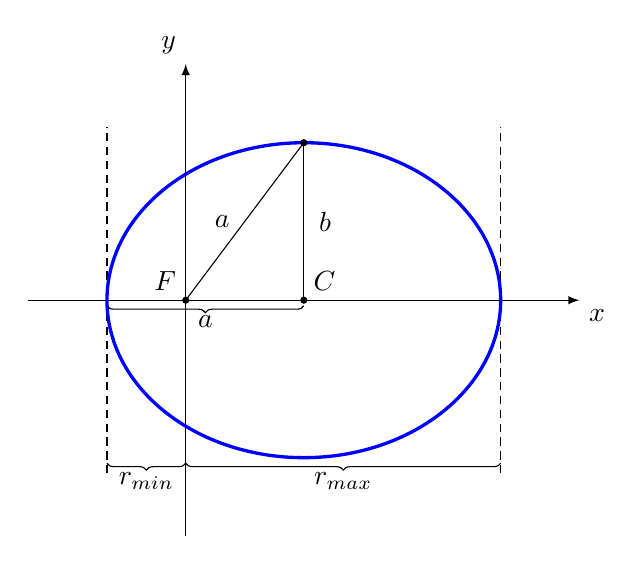
\begin{tikzpicture}
     \draw[-latex] (-2,0) -- (5,0) node[below right] {$x$};
     \draw[-latex] (0,-3) -- (0,3) node[above left] {$y$};
     \draw[densely dashed] (-1,-2.2) -- (-1,2.2);
     \draw[densely dashed] (4,-2.2) -- (4,2.2);
     \draw[blue,line width=1.2pt] (1.5,0) ellipse (2.5 and 2);
     \fill (1.5,0) circle (1.3 pt) node[above right] {$C$};
     \fill (0,0) circle (1.3 pt) node[above left] {$F$};
     \fill (1.5,2) circle (1.3 pt);
     \draw[decorate,decoration={brace,raise=2pt,mirror}] (-1,0) -- node[below=2pt]{$a$} (1.5,0);
     \draw (1.5,2) -- node[right=2pt]{$b$} (1.5,0);
     \draw (0,0) -- node[left=2pt]{$a$} (1.5,2);
     \draw[decorate,decoration={brace,mirror,raise=2pt}] (-1,-2) -- node[below=2pt]{$r_\text{min}$} (0,-2);
     \draw[decorate,decoration={brace,mirror,raise=2pt}] (0,-2) -- node[below=2pt]{$r_\text{max}$} (4,-2);
    \end{tikzpicture}
    \caption{A kapott ellipszispálya.
   A nagytengely hossza $a$ a kistengelyé $b$.
   Az origó az egyik fókusz ($F$), míg $C$ a centrum.
   Az origótól való legkisebb távolság $r_\text{min}$, a legnagyobb pedig $r_\text{max}$.}\label{fig:A13-ellipszis}
   \end{figure}
   Forgassuk el a koordináta-rendszert, hogy $\beta=0$ legyen.
   A legnagyobb és a legkisebb távolság, illetve a nagytengely hossza:
   \al{
    &r_\text{max}=\frac{p}{1-e}
    &r_\text{min}=\frac{p}{1+e}
    &&a=\frac{r_\text{max}+r_\text{min}}{2}
       =\frac{p}{1-e^2}.
   }
   A fókusz centrumtól mért távolsága, és a kistengely hossza:
   \al{
    &a-r_\text{min}=\frac{ep}{1-e^2}=e\cdot a.
    &b=\sqrt{a^2-(e\cdot a)^2}=\sqrt{a^2(1-e^2)}=\sqrt{a\cdot p},
   }
   amellyel a terület:
   \al{
    A=\pi ab =\pi\sqrt{a^3 p}.
   }
   A súrolt terület a területi sebesség és a periódusidő szorzataként is előáll (Kepler II{.}):
   \al{
    &\pi\sqrt{a^3 p}=T\cdot \frac{L}{2m}
    &\frac{T^2}{a^3}
      =\frac{4m^2\pi^2}{L^2}p
      =\frac{4m^2\pi^2}{L^2}\frac{L^2}{m\alpha}
      =\frac{4m\pi^2}{\alpha}
      =\text{állandó}.
   }
   Ez Kepler III.\ törvénye.
   Bolygómozgásnál $\alpha=mM\gamma$, így ott $\frac{T^2}{a^3}=\frac{4\pi^2}{M\gamma}$.
   A keringési idő bolygómozgásra:
   \al{
    T
    &=\sqrt{a^3\frac{4\pi^2}{M\gamma}}
     =\sqrt{\left(\frac{p}{1-e^2}\right)^3\frac{4\pi^2}{M\gamma}}
     =\sqrt{\left(\frac{\frac{L^2}{\gamma m^2 M}}{\frac{2\abs{E}L^2}{m\gamma^2 m^2 M^2}}\right)^3\frac{4\pi^2}{M\gamma}}
     =\sqrt{\left(\frac{m\gamma M}{2\abs{E}}\right)^3\frac{4\pi^2}{M\gamma}}\\
    &=\pi \gamma mM \sqrt{\frac{m}{2\abs{E}^3}}.
   }
 
 \section{Elektrodinamika} 
  
  \subsection{Coulomb-törvény kapcsolata a Maxwell-egyenletekkel}
   
   Lásd \ref{ss:01-CoulombMaxwell}. fejezet.
   
  \subsection{Oszcilláló töltéseloszlás tere}\label{ss:13-oszcillaloter}
   
   Tekintsünk olyan rendszert, ahol a potenciálok lokalizáltak (kiterjedése $d$), és szinuszosak: $\psi(\omega,\rv)$, $\Av(\omega,\rv)\sim e^{-i\omega t}$.
   Lorentz-mértékben: $0=\divo{\Av}+\frac{1}{c^2}\partial_t\phi=\divo{\Av}-\frac{1}{c^2}i\omega\phi$ így elég csak $\Av$-t kiszámítani, abból $\phi$ adódik.
   
   A retardált potenciálok (\ref{ss:9-retpot}. fejezet, illetve \eqref{eq:09-retpotA} egyenlet) szerint:
   \al{
    \vect{A}(t,\rv)
      &=\frac{\mu_0}{4\pi}\intl{}{}\dd^3\rv'\,\frac{\vect{J}\left(t-\frac{\abs{\rv-\rv'}}{c},\rv'\right)}{\abs{\rv-\rv'}}
       =\frac{\mu_0}{4\pi}\intl{}{}\dd^3\rv'\,\frac{\vect{J}(\rv')e^{-i\omega\left(t-\frac{\abs{\rv-\rv'}}{c}\right)}}{\abs{\rv-\rv'}}\\
    \vect{A}(\omega,\rv)
      &=\frac{\mu_0}{4\pi}\intl{}{}\dd^3\rv'\,\frac{\vect{J}(\rv')e^{ik\abs{\rv-\rv'}}}{\abs{\rv-\rv'}}
   }
   
   Közeltérben ($d\ll r\ll\lambda$), ahol $k\abs{\rv-\rv'}\ll 1$, nem számít a retardálás.
   A hullámzónában ($d\ll\lambda\ll r $) csak az $\sim\frac{1}{r}$ tagokat tartjuk meg:
   \al{
    \frac{1}{\abs{\rv-\rv'}}&=\frac{1}{r}+\mathcal{O}\left(\frac{d}{r^2}\right),\\
    \abs{\rv-\rv'}
      &=\sqrt{\rv^2-2\rv\rv'+\rv'^2}
      =r\sqrt{1-2\frac{\rv\rv'}{r^2}+\frac{\rv'^2}{\rv^2}}
      =r\sqrt{1-2\frac{\rv\rv'}{r^2}}+\mathcal{O}\left(\frac{d^2}{r}\right)\\
      &=r\left(1-\frac{\rv\rv'}{r^2}\right)+\mathcal{O}\left(\frac{d^2}{r}\right)
       =r-\rv'\ev_\rv+\mathcal{O}\left(\frac{d^2}{r}\right)\\
    e^{ik\abs{\rv-\rv'}}
      &\approx e^{ik(r-\rv'\ev_\rv)}
       =e^{ikr}e^{-ik\rv'\ev_\rv}
       \approx
        e^{ikr}\left(1-ik\rv'\ev_\rv\right),
   }
   az utolsó tagban felhasználtuk, hogy $k\abs{\rv'}<kd\ll 1$
   Így
   \aln{
    \vect{A}(\omega,\rv)
      &=\frac{\mu_0}{4\pi}\frac{e^{ikr}}{r}\intl{}{}\dd^3\rv'\,\vect{J}(\rv')\big(1-ik\rv'\ev_\rv\big)\label{eq:13-vectpot}
   }
    
   \paragraph{Mozgó töltés sugárzása}\label{ss:14-mogotoltessugarzasa}
    
    Tekintsünk egy ponttöltés, amely  általános mozgást végez: $\Jv(\rv)=q\vv(t)\delta\big(\rv-\vects{\gamma}(t)\big)$, ahol $\vects{\gamma}(t)$ a pálya. $\frac{1}{r}$-ed rendben \eqaref{eq:09-retpotA} egyenlet kiintegrálható:
    \al{
     \vect{A}(t,\rv)
      &\approx\frac{\mu_0}{4\pi}\intl{}{}\dd^3\rv'\,\frac{1}{r}q\vv(t)\delta\big(\rv'-\vects{\gamma}(t)\big)
       =\frac{\mu_0}{4\pi r}q\vv\left(t-\frac{r}{c}\right).
    }
    A deriválásnál is csak $\frac{1}{r}$-ed rendig tartjuk meg a tagokat, így $\vects{\nabla}\to-\frac{1}{c}\grad{r}\partial_t=-\frac{\rv}{rc}\partial_t=-\frac{\ev_\rv}{c}\partial_t$.
   A terek:
    \al{
     \Bv
      &=\rot{\Av}
       =\frac{q\mu_0}{4\pi}\rot{\vv\left(t-\frac{r}{c}\right)}
       =-\frac{q\mu_0}{4\pi c}\ev_\rv\times\partial_t\vv\left(t-\frac{r}{c}\right)
       =\frac{q\mu_0}{4\pi r c}\left[\av\left(t-\frac{r}{c}\right)\times\ev_\rv\right]  \\
     \dot{\Ev}
      &=c^2\rot{\Bv}
       =c^2\frac{q\mu_0}{4\pi r^2 c^2}\left[\dot{\av}\left(t-\frac{r}{c}\right)\times\ev_\rv\right]\times\ev_\rv\\
     \Ev
      &=\frac{q\mu_0}{4\pi r^2 }\left[\av\left(t-\frac{r}{c}\right)\times\ev_\rv\right]\times\ev_\rv
       =Z_0\Hv\times\ev_\rv.
    }
    A kisugárzott teljesítménysűrűség:
    \al{
     \Sv
      &=\Ev\times\Hv
       =Z_0(\Hv\times\ev_\rv)\times\Hv
       =Z_0\Hv^2\ev_\rv
       =Z_0\frac{q^2}{16\pi^2 r^2 c^2}\left[a\left(t-\frac{r}{c}\right)\right]^2\sin^2\vartheta\ev_\rv,
    }
    ahol $Z_0=\mu_0 c$ a vákuum ellenállása.
   Innen
    \aln{
     &\der{P}{\Omega}=\frac{Z_0 q^2}{16\pi^2 c^2}\left[a\left(t-\frac{r}{c}\right)\right]^2\sin^2\vartheta,
     &P=\frac{Z_0 q^2}{6\pi c^2}\left[a\left(t-\frac{r}{c}\right)\right]^2.\label{eq:13-Larmor}
    }
    Ez a Larmor-képlet.
   Látjuk, hogy a gyorsuló töltés sugároz.
   A képlet akkor használható, ha $d\ll \lambda\Leftrightarrow \frac{d}{\delta t}\ll \frac{\lambda}{\delta t}\Leftrightarrow v\ll c$, vagyis a nem relativisztikus határesetben.
    
    Körmozgásra $a\left(t-\frac{r}{c}\right)=\frac{v^2}{R}$:
    \al{
     P=\frac{Z_0 q^2}{6\pi c^2}\frac{v^4}{R^2}
      =\frac{Z_0 q^2 c^2}{6\pi R^2}\left(\frac{v}{c}\right)^4.
    }
    
   \paragraph{Sugárzás relativisztikus tárgyalása, Ciklotron sugárzás} 
    
    A relativisztikus tárgyaláshoz a Larmor-képletet relativisztikusan invariáns alakban kell felírni.
     
    A bal oldalon a teljesítmény $P=\der{E}{t}$, melyhez álló rendszerben $c\minv{p}^\mu=(E,0)$, és $\minv{x}^\mu=(ct,0)$.
   Mozgó rendszerbe való áttérésnél: $E\to E'=\frac{E}{\sqrt{1-v^2/c^2}}$ és $t\to t'=\frac{t}{\sqrt{1-v^2/c^2}}$, ahonnan: $\det{E}{t}=\der{E'}{t'}$, vagyis invariáns. 
    
    A jobb oldalon $\vect{a}$ nem kovariáns.
   A $v\to 0$ limesz ismeretében azzá tehetjük:
    \al{
     \minv{a}^\mu
      &=\der{^2\minv{r}^\mu}{^2\tau}
       =\der{}{\tau}\left(\frac{c}{\sqrt{1-\frac{v^2}{c^2}}},\frac{\vv}{\sqrt{1-\frac{v^2}{c^2}}}\right)
       =\frac{1}{\sqrt{1-\frac{v^2}{c^2}}^2}\left(0,\av\right)
        +\left(c,\vv\right)\der{}{\tau}\frac{1}{\sqrt{1-\frac{v^2}{c^2}}}\\
      &=\frac{1}{\sqrt{1-\frac{v^2}{c^2}}^2}\left(0,\av\right)
        +\frac{\vv\av}{c^2}\frac{1}{\sqrt{1-\frac{v^2}{c^2}}^4}\left(c,\vv\right)
       =\left(\frac{\vects{\beta}\av}{\sqrt{1-\frac{v^2}{c^2}}^4},\frac{\av}{\sqrt{1-\frac{v^2}{c^2}}^2}+\frac{(\vects{\beta}\av)\vects{\beta}}{\sqrt{1-\frac{v^2}{c^2}}^4}\right)\\
      &=\big(\gamma^4\vects{\beta}\av,\gamma^2\av+(\vects{\beta}\av)\vects{\beta}\gamma^4\big),
    }
    ami tudja, hogy $\minv{a}^\mu\to (0,\av)$, illetve $\minv{a}^\mu \minv{a}_\mu\to -\av^2$.
   Ezzel a Larmor-képlet felírva:
    \al{
     P=-\frac{Z_0 q^2}{6\pi c^2}\minv{a}^\mu \minv{a}_\mu,
    }
    szembeötlően invariáns.
   Visszaírjuk a gyorsulást és a sebességet:
    \al{
     \minv{a}^\mu\minv{a}_\mu
     &=\gamma^8(\vects{\beta}\av)^2-\gamma^4\av^2-(\vects{\beta}\av)^2\vects{\beta}^2\gamma^8-2\gamma^6(\vects{\beta}\av)^2\\
     &=-\gamma^4\av^2-\gamma^6(\vects{\beta}\av)^2+\gamma^6(\vects{\beta}\av)^2\Big[\underbrace{\gamma^2\big(1-\vects{\beta}^2\big)}_{=1}-1\Big]
      =-\gamma^4\av^2-\gamma^6(\vects{\beta}\av)^2.
    }
    Ez $\vv\to 0$-ra, visszaadja $-\av^2$-et, így a fenti kifejezés megfelel a klasszikus határesetnek.
   Alakítsuk még egy kicsit:
    \al{
     \minv{a}^\mu\minv{a}_\mu
      &=-\gamma^4\av^2-\gamma^6(\vects{\beta}\av)^2
       =-\gamma^6\big[(1-\betav^2)\av^2+(\vects{\beta}\av)^2\big]
       =-\gamma^6\big[\av^2+(\vects{\beta}\av)^2-\av^2\betav^2\big]\\
      &=-\gamma^6\big[\av^2+(\vects{\beta}\times\av)^2\big].
    }
    Ezzel tehát a Larmor-formula relativisztikus megfelelője:
    \al{
     P=\frac{Z_0 q^2}{6\pi c^2}\gamma^6\big[\av^2+(\vects{\beta}\times\av)^2\big].
    }
    Körmozgás esetén $\betav\perp\av$, így $(\vects{\beta}\times\av)^2=a^2\beta^2$, vagyis:
    \al{
     P=\frac{Z_0 q^2}{6\pi c^2}\gamma^6\big[(1-\beta^2)a^2\big]
      =\frac{Z_0 q^2}{6\pi c^2}\gamma^4 a^2.
    }
    A klasszikus képletet képest ez egy $\gamma^4$-es faktorban tér el.
   Ha $v\sim c$, akkor a sugárzás teljesítménye nagyon megnő.

 \section{Kvantummechanika}
  
  \subsection{Kötött állapot} 
   
   Kötött állapotról akkor beszélünk, ha a rendszer spektruma pontspektrum.
   Ekkor a hullámfüggvény normálható, és az eleme a négyzetesen integrálható függvények Hilbert-terének.
   
  \subsection{Schrödigner-egyenlet centrális erőtérben}
   
   Legyen a potenciál centrális, azaz $\opV(\oprv)=\opV(\opr)$.
   Ekkor a Schrödinger-egyenlet gombi koordinátákban, koordinátareprezentációban:
   \al{
    \left\{-\frac{\hbar^2}{2m}\left[\frac{1}{r}\partial_r^2r+\frac{1}{r^2}\left(\partial_{\vartheta}+\frac{1}{\tg{\vartheta}}\partial_{\vartheta}^2+\frac{1}{\sin^2{\varphi}}\partial_{\vartheta}^2\right)\right]+V(r)\right\}\psi(r,\vartheta,\varphi)=E\psi(r,\vartheta,\varphi).
   }
   Az 
   \al{
    L^2=-\hbar^2\left(\partial_{\vartheta}^2+\frac{1}{\tg{\vartheta}}\partial_{\vartheta}+\frac{1}{\sin^2{\vartheta}}\partial_{\varphi}^2\right)
   }
   sajátérték problémájának megoldását lásd \ref{ss:06-L2spme}. fejezet.
   A megoldást akkor keressük
   \al{
    \psi(r,\vartheta,\varphi)=\frac{1}{r}R(r)Y_l^m(\vartheta,\varphi)
   }
   alakban, melyet behelyettesítve az egyenletbe a radiális Schrödinger-egyenletet kapjuk:
   \aln{
    \left[-\frac{\hbar^2}{2m}\frac{1}{r}\partial_r^2r+\frac{\hbar^2 l(l+1)}{2mr^2}+V(r)\right]\psi(r,\vartheta,\varphi)&=E\psi(r,\vartheta,\varphi)\nonumber\\
    \left[-\frac{\hbar^2}{2m}\der{^2}{r^2}+\frac{\hbar^2 l(l+1)}{2mr^2}+V(r)\right]R(r)&=ER(r).\label{eq:13:radSch}
   }
   
  \subsection{Hidrogénatom}
   
   Legyen $V(r)=-\frac{kZe^2}{r}$.
   Az állapotok negatív energiájúak: $E=-\abs{E}$.
   Ezzel az egyenlet:
   \al{
    0=\left[-\frac{\hbar^2}{2m}\der{^2}{r^2}+\frac{\hbar^2 l(l+1)}{2mr^2}-\frac{kZe^2}{r}+\abs{E}\right]R(r).
   }
   Bevzetjük az alábbi jelöléseket:
   \al{
    &r_0=\frac{\hbar}{\sqrt{2m\abs{E}}}
    &\xi=\frac{\sqrt{8m\abs{E}}}{\hbar}r=\frac{2r}{r_0}
    &&a_0=\frac{\hbar^2}{mke^2}
    &&\ep=\frac{Zke^2\sqrt{2m\abs{e}}}{2\hbar\abs{E}},
   }
   melyekkel
   \al{
    \der{^2R(\xi)}{\xi^2}+\left[-\frac{1}{4}+\frac{\ep}{\xi}-\frac{l(l+1)}{\xi^2}\right]R(\xi)=0.
   }
   
   \paragraph{Sommerfeld polinommódszer}
    
    Először megkeressük az aszimptotikus megoldást:
    \al{
     &\xi\to 0
     &\der{^2R(\xi)}{\xi^2}-\frac{l(l+1)}{\xi^2}R(\xi)=0
     &&R(\xi)\sim\xi^{l+1},\\
     &\xi\to \infty
     &\der{^2R(\xi)}{\xi^2}-\frac{1}{4}R(\xi)=0
     &&R(\xi)\sim e^{-\frac{1}{2}\xi}.
    }
    
    A megoldást keressük egy polinom és az aszimptotikus megoldás szorzataként: $R(\xi)=u(\xi)e^{-\frac{1}{2}\xi}$, mellyel
    \al{
     &\dd_\xi R(\xi)=\left(-\frac{1}{2}u(\xi)+u'(\xi)\right)e^{-\frac{1}{2}\xi}
     &\dd_\xi^2 R(\xi)=\left(\frac{1}{4}u(\xi)-u'(\xi)+u''(\xi)\right)e^{-\frac{1}{2}\xi},
    }
    így
    \al{
     u''(\xi)-u'(\xi)+\left[\frac{\ep}{\xi}-\frac{l(l+1)}{\xi^2}\right]u(\xi)=0.
    }
    A hatványsor legyen $u(\xi)=\xi^s\suml{i=0}{\infty}c_i\xi^i$, ahol $s$ az iniciális index.
   Ennek deriváltjai:
    \al{
     u'(\xi)&=\suml{i=0}{\infty}(i+s)c_i\xi^{i+s-1}
      =\suml{i=1}{\infty}(i+s-1)c_{i-1}\xi^{i+s-2}\\
     u''(\xi)&=\suml{i=0}{\infty}(i+s)(i+s-1)c_i\xi^{i+s-2},
    }
    majd behelyettesítve:
    \al{
     0
      &=\suml{i=0}{\infty}(i+s)(i+s-1)c_i\xi^{i+s-2}-\suml{i=1}{\infty}(i+s-1)c_{i-1}\xi^{i+s-2}+\left[\frac{\ep}{\xi}-\frac{l(l+1)}{\xi^2}\right]\suml{i=0}{\infty}c_{i}\xi^{i+s}\\
      &=s(s-1)c_0\xi^{s-2}+\suml{i=1}{\infty}\bigg(
       (i+s)(i+s-1)c_i\xi^{i+s-2}
      -(i+s-1)c_{i-1}\xi^{i+s-2}\bigg)\\
      &\qquad\qquad\qquad+\suml{i=0}{\infty}\left[\ep c_{i}\xi^{i+s-1}-l(l+1)c_{i}\xi^{i+s-2}\right]\\
      &=\big[s(s-1)-l(l+1)\big]c_0\xi^{s-2}+\suml{i=1}{\infty}\bigg(
        \big[(i+s)(i+s-1)-l(l+1)\big]c_i\\
      &\qquad\qquad\qquad\qquad\qquad\qquad\qquad\qquad\qquad\qquad\qquad\qquad
        +\big[\ep-(i+s-1)\big]c_{i-1}\bigg)\xi^{i+s-2}.
    }
    Ennek mindegyik együtthatója el kell, hogy tűnjön. $c_0\ne 0$, mert biztos van egy olyan $c_i$, így $s=l+1$ vagy $s=-l$, ahonnan csak az első jön szóba, a $\xi\to 0$-ban való regularitás miatt.
   A többi együtthatóra:
    \al{
     c_i
      =\frac{-\ep+(i+s-1)}{(i+s)(i+s-1)-l(l+1)}c_{i-1}
      =\frac{-\ep+i+l}{i(i+2l+1)}c_{i-1}.
    }
    Nagy $i$-re $\frac{c_i}{c_{i-1}}\sim\frac{1}{i}$, ami így azt eredményezné, hogy $u\sim e^{\xi}$, vagyis $R(\xi)\sim e^{\frac{1}{2}\xi}$, ami nem reguláris.
   Emiatt léteznie kell egy $i_\text{max}$-nak, hogy $c_{i_\text{max}}=0$.
   Ekkor 
    \al{
     i_\text{max}+l-\ep=0.
    }
    Bevezetjük az
    \al{
     n=i_\text{max}+l=\ep,
    }
    főkvantumszámot, ami: $n>l$, $n=1,2,3,\dots$, illetve $n=\frac{Z r_0}{a_0}$.
   Az eredmény összefoglalva:
    \al{
     E_n
      &=-\frac{\hbar^2}{2m r_0^2}
       =-\frac{Z^2\hbar^2}{2m a_0^2}\frac{1}{n^2}
       =-\frac{mZ^2 k^2e^4}{2\hbar^2}\frac{1}{n^2}
       =-\frac{mZ^2e^4}{32\pi^2\ep_0^2\hbar^2}\frac{1}{n^2},
    }
    \al{
     \psi(r,\vartheta,\varphi)
      &=
       \sqrt{{\left (\frac{2}{r_0} \right ) }^3\frac{(n-l-1)!}{2n\,(n+l)!} } 
       \left(\frac{2r}{r_0}\right)^l L_{n-l-1}^{2l+1}\left(\frac{2r}{r_0}\right)e^{-\frac{r}{r_0}}Y_l^m(\vartheta,\varphi),
    }
    ahol $L_{n-l-1}^{2l+1}\left(\frac{2r}{r_0}\right)$ az asszociált Laguerre-polinomok:
    \al{
     L_n^{\alpha}(x)=\frac{x^{-\alpha} e^x}{ n!}\frac{d^n}{dx^n} \left(e^{-x} x^{n+\alpha}\right).
    }
    \begin{figure}[ht!]
     \centering
    \subfloat[$n=1$\label{fig:A13-e1}]{\includegraphics[width= 0.3\textwidth]{./A13tetel/H-n1}} \hspace{6pt}
    \subfloat[$n=2$\label{fig:A13-e2}]{\includegraphics[width= 0.3\textwidth]{./A13tetel/H-n2}} \hspace{6pt}
    \subfloat[$n=3$\label{fig:A13-e3}]{\includegraphics[width= 0.3\textwidth]{./A13tetel/H-n3}}
     \caption{Radiális valószínűségek ($w_{n,l}(r)=\abs{\Psi_r(r)}^2\cdot r^2$) az első három energiaszinthez tartozó hullámfüggvények esetében. (Az $y$ tengely skálája változik az ábrákon!)}
    \end{figure}

  \chapter{Mozg\'as centr\'alis er\H{o}t\'erben: Sz\'or\'asi folyamatok}
 
 \section{Mechanika} 
  
  \subsection{Kéttestprobléma} 
   
   Vizsgáljunk két tömegponttot, amelyek csak egymásra hatnak.
   A mozgásegyenletek:
   \al{
    &m_1\ddot\rv_1=\Fv_{12}
    &m_2\ddot\rv_2=\Fv_{21}
    &&\Fv_{12}=-\Fv_{21}.
   }
   A két egyenlet összege: $0=\dd_t^2(m_1\rv_1+m_2\rv_2)$, vagyis az $\Rv=\frac{m_1\rv_1+m_2\rv_2}{m_1+m_2}$ pont egyenes vonalú egyenletes mozgást végez.
   Ez a tömegközéppont megmaradásának tétele.
   Rögzítsük az origót ehhez a ponthoz.
   Ekkor $m_1\rv_1+m_2\rv_2=0$.
   
   Vezessük le a különbségi koordinátára ($\rv=\rv_2-\rv_1$) egy mozgásegyenletet.
   A két mozgásegyenletet a másik tömegekkel bővítve majd kivonva:
   \al{
    m_1 m_2(\ddot\rv_2-\ddot\rv_1)&=-m_2\Fv_{21}+m_1\Fv_{12}=(m_1+m_2)\Fv_{12}\\
    \frac{m_1 m_2}{m_1+m_2}\ddot\rv&=\Fv_{12}.
   } 
   ahol $\mu=\frac{m_1 m_2}{m_1+m_2}$ a redukált tömeg.
   A problémát visszavezettük egy egyrészecske problémára.
   A tömegközépponti rendszerben a két tömegpont koordinátája ezzel:
   \al{
    &\rv_1=-\rv\frac{m_2}{m_1+m_2}
    &\rv_2=\rv\frac{m_1}{m_1+m_2}.
   } 
   
   Ezzel pl. a Kepler-probléma esetében figyelembe vehető, hogy a Nap nem rögzített.
   A kapott eredményben szereplő $m$ nem a Föld tömege, hanem a redukált tömeg. 
   
  \subsection{Szórásszámítás}
   
   Legyen az origóban egy szórócentrum, amely által létrehozott centrális potenciálban mozog a szóródó részecske.
   Aszimptotikus távolságban a mozgás egyenes vonalú egyenletes.
   Kérdés, hogy mekkora lesz a szórás után aszimptotikus távolságban a kilépő részecske pályájának elhajlása a bemenő pályához képest. 
   
   A mozgás során megmaradó mennyiségek:
   \begin{itemize}
    \item az energia, ha az ütközés rugalmas,
    \item az összimpulzus, ha nincs külső erő,
    \item a impulzusmomentum
    \item a tömegkközéppont.
   \end{itemize}
   
   A beérkező részecske energiája aszimptotikus távolságban: $E=\frac{1}{2}m^2 v_\infty^2$, impulzusmomentuma $L=m\rho v_\infty$, ahol $\rho$ az asziptotikus pálya és az origó távolsága. $\rho$ az ütközési paraméter, ettől függ, hogy milyen $\chi$ szögben fog szóródni a kilépő részecske.
   A $\rho(\chi)$ függvényt keressük meg. 
   
   A belépő részecskefluxus $n$ (darab/felület/másodperc), mellyel a részecskeáram (da\-rab/má\-sod\-perc) a $\rho$ sugarú $\dd\rho$ széles gyűrűn: $\dd N=n2\pi\rho\dd\rho$.
   Ezek a részecskék fognak ugyanabba a $\chi$ szögbe szóródni.
   A térszög, ami ehhez tartozik: $\dd\Omega=\frac{1}{r^2}2\pi r\sin\chi r\dd\chi=2\pi\sin\chi\dd\chi$.
   Bevezetjük azt az arányt, ami azt jellemzi, hogy a részecskék mekkora része szóródik $\dd\chi$ szögben:
   \aln{
    \dd\sigma
     =\frac{\dd N}{n}
     =2\pi\rho\dd\rho
     =2\pi\rho\abs{\der{\rho}{\chi}}\dd\chi
     =2\pi\rho\abs{\der{\rho}{\chi}}\frac{\dd\Omega}{2\pi\sin\chi}
     =\frac{\rho}{\sin\chi}\abs{\der{\rho}{\chi}}\dd\Omega.\label{eq:14-dhatkm}
   }
   A $\der{\sigma}{\Omega}$ a differenciális szórási hatáskeresztmetszet, mértékegysége $\mathrm{m}^2$. 
   
   \paragraph{Példa: tömör, $R$ sugarú gömb}
    
    Szórás akkor történik, ha $\rho\leq R$.
   Ekkor a szórás szöge $\chi$, ami a beesés szögével kifejezhető $\chi=\pi-2\varphi$. 
    \al{
     \rho
      =R\sin\varphi
      =R\sin\left(\frac{\pi-\chi}{2}\right)
      =R\cos\left(\frac{\chi}{2}\right).
    }
    Ezzel
    \al{
     \der{\sigma}{\Omega}
      =\frac{\rho}{\sin\chi}\abs{\der{\rho}{\chi}}
      =\frac{R\cos\left(\frac{\chi}{2}\right)}{\sin\chi}\abs{\der{}{\chi}R\cos\left(\frac{\chi}{2}\right)}
      =\frac{R^2}{2}\frac{\cos\left(\frac{\chi}{2}\right)}{\sin\chi}\sin\left(\frac{\chi}{2}\right)
      =\frac{R^2}{4}\frac{\sin\left(\chi\right)}{\sin\chi}
      =\frac{R^2}{4},
    }
    így
    \al{
     \sigma=\frac{R^2}{4}\cdot 4\pi=R^2\pi.
    } 
    Tehát a gömb szórási hatáskeresztmetszete megegyezik a gömb keresztmetszetével.
    
  \subsection{Rutherford szórás}
   
   Lásd \aref{ss:13-palyaegyenlete}. fejezetben.
   A lehetséges pályákat \aref{fig:A14-palyak}. ábra mutatja.
   
   \begin{figure}[ht!]
    \centering
    \includegraphics[width=0.35\textwidth]{A14tetel/palyak}
    \caption{A szórócentrum az origóban van.
   Vonzó kölcsönhatás esetén a bal oldali hiperbola ág mutatja a pályát.
   Taszító kölcsönhatás esetén a jobb oldali pálya valósul meg.
   Az ütközési paraméter ($\rho$) a két aszimptota távolsága az origótól.}\label{fig:A14-palyak}
   \end{figure}

   Rögzítjük a $q_1$ töltést, $q_2$ töltést pedig szóratjuk a $q_1$ terén.
   Legyen a töltés taszító, ekkor $\alpha=-k q_1 q_2$.
   Ekkor a hiperbola megfordul, így az egyenlete:
   \al{
    &r(\varphi)=\frac{-\abs{p}}{1-e\cos(\varphi)}
    &p=\frac{L^2}{m\alpha}=-\frac{m v_\infty^2 \rho^2}{\abs{\alpha}}
    &&e=\sqrt{1+\frac{2EL^2}{m\alpha^2}}
       =\sqrt{1+\left(\frac{m  \rho v_\infty^2}{\alpha}\right)^2}.
   }
   
   A két aszimptota a $\varphi_{1,2}=\pm\arccos{\frac{1}{e}}$-nél van, így a szórási szög:
   \al{
    \chi
     &=\pi-(\varphi_1-\varphi_2)
      =\pi-2\arccos\frac{1}{e}
      =2\left(\frac{\pi}{2}-\arccos\frac{1}{e}\right)
      =2\arcsin\frac{1}{e}\\
    \sin\frac{\chi}{2}
     &=\frac{1}{e}
      =\frac{1}{\sqrt{1+\left(\frac{m  \rho v_\infty^2}{\alpha}\right)^2}}\\
     \rho(\chi)
      &=\frac{\abs{\alpha}}{m v_\infty^2}\sqrt{\frac{1}{\sin^2\frac{\chi}{2}}-1}
       =\frac{\abs{\alpha}}{m v_\infty^2}\frac{1}{\tg\frac{\chi}{2}},
   }
   ahonnan a differenciális hatáskeresztmetszet:
   \al{
    \der{\sigma}{\Omega}
     &=\frac{\rho}{\sin\chi}\abs{\der{\rho}{\chi}}
      =\frac{\alpha^2}{m^2 v_\infty^4}\frac{1}{\sin\chi}\frac{1}{\tg\frac{\chi}{2}}\abs{\der{}{\chi}\frac{1}{\tg\frac{\chi}{2}}}
      =\frac{\alpha^2}{m^2 v_\infty^4}\frac{1}{\sin\chi}\frac{1}{\tg\frac{\chi}{2}}\frac{1}{2}\frac{1}{\sin^2\frac{\chi}{2}}\\
     &=\frac{\alpha^2}{m^2 v_\infty^4}\frac{1}{2\sin^2\frac{\chi}{2}}\frac{1}{2}\frac{1}{\sin^2\frac{\chi}{2}}
      =\left(\frac{\alpha}{2m v_\infty^2}\right)^2\frac{1}{\sin^4\frac{\chi}{2}},
   }
   melyből a teljes szórási hatáskeresztmetszet:
   \al{
    \sigma
     &=\intl{}{}\dd\Omega\,\left(\frac{\alpha}{2m v_\infty^2}\right)^2\frac{1}{\sin^4\frac{\chi}{2}}
      =\left(\frac{\alpha}{2m v_\infty^2}\right)^2\intl{0}{\pi}\dd\chi\,2\pi\sin\chi\frac{1}{\sin^4\frac{\chi}{2}}\\
     &=\left(\frac{\alpha}{2m v_\infty^2}\right)^2 4\pi\intl{0}{\pi}\dd\chi\,\frac{\cos\frac{\chi}{2}}{\sin^3\frac{\chi}{2}}
      =\left(\frac{\alpha}{2m v_\infty^2}\right)^2 4\pi\left[-\frac{1}{\sin^2\frac{\chi}{2}}\right]_{0}^{\pi}
      =\text{divergens!}
   }
   
   Ez nem meglepő, a Coulomb-potenciál $\sim\frac{1}{r}$-es, azaz végtelen hatótávolságú.
   A kísérleti eredményekkel ez ott egyeztethető össze, hogy itt nem vettük figyelembe az árnyékolást, pl. szilárdtestekben való szóródásnál a szóró potenciálra sokkal reálisabb közelítés a $\sim\frac{e^{-r/r_0}}{r}$ alak, aminek hatótávolsága véges, így szórási hatáskeresztmetszete is az.
   
   Megjegyzés: a kvantummechanikai szóráselmélet is a Rutherford-féle formulát adja, a differenciális hatáskeresztmetszetre levezetett összefüggés a kvantummechanikában is helytálló. 
   
 \section{Kvantummechanika}
  
  \subsection{Potenciálszórás}
   
   A kéttest ütközések visszavezethetőek egyrészecske problémára, így a szórásokat úgy vizsgáljuk, hogy egy részecskét szóratunk fix potenciálon.
   A kísérletileg mérhető differenciális hatáskeresztmetszetet szeretnénk meghatározni a rendszer tulajdonságaiból.
   
   Essen egy monokromatikus $\kv_i$ hullámszámú részecske a szórócentrumra.
   A potenciál legye rövid hatótávolságú, vagyis $V(\rv)\sim\frac{1}{r^{1+\ep}}$, ahol $\ep>0$.
   A radiális Schrödinger-egyenlet $r\to\infty$ aszimptotikus megoldása $\mathcal{O}\left(\frac{1}{r}\right)$ rendig:
   \aln{
    \psi(k,\rv)=A\bigg(\underbrace{e^{i\kv_i\rv}}_{\text{be}}+\underbrace{f(\vartheta,\varphi)\frac{e^{i k r}}{r}}_{\text{szórt}}\bigg)
     =\psi_\text{be}(\rv)+\psi_\text{ki}(\rv,k),\label{eq:14-aszimptotikuspsi}
   }
   aminek az első tagja a beeső $\kv_i$ impulzusú síkhullám, a második tagja pedig egy kifutó gömbhullám.
   
   Számoljuk ki a detektoron ($r\to\infty$) a szórási folyamat nélkül beeső hullám, illetve a szórócentrum jelenlétében mérhető részecskeáram-sűrűségének hányadosát.
   Ebből a deifferenciális haráskeresztmetszet számolható lesz.
   
   A részecskeáram-sűrűség:
   \al{
    \jv(\rv)
     &=\Re\left[\frac{\hbar}{mi}\psi^*(\rv)\grad{\psi(\rv)}\right],
   }
   ahol $\grad=\frac{\partial }{\partial r}\ev_r+\frac{1}{r}\frac{\partial }{\partial \vartheta}\ev_\vartheta+\frac{1}{r \sin\vartheta}\frac{\partial }{\partial \phi}\ev_\varphi\xrightarrow{r\to\infty}\frac{\partial }{\partial r}\ev_r$, így
   \al{
    \jv(\rv)
     &=\Re\left[\frac{\hbar}{mi}\big(\psi^*_\text{be}(\rv)+\psi^*_\text{ki}(\rv,k)\big)\frac{\partial }{\partial r}\ev_r\big(\psi_\text{be}(\rv)+\psi_\text{ki}(\rv,k)\big)\right]\\
     &=\underbrace{\Re\left[\frac{\hbar}{mi}\psi^*_\text{be}(\rv)\grad\psi_\text{be}(\rv)\right]}_{\jv_\text{be}(\rv)}
      +\underbrace{\Re\left[\frac{\hbar}{mi}\psi^*_\text{ki}(\rv,k)\frac{\partial }{\partial r}\psi_\text{ki}(\rv,k)\right]}_{j_\text{sz}(\rv)}\ev_r\\
     &\qquad\qquad+\underbrace{\Re\left[\frac{\hbar}{mi}\left(\psi^*_\text{be}(\rv)\frac{\partial }{\partial r}\psi_\text{ki}(\rv,k)+\psi^*_\text{ki}(\rv,k)\frac{\partial }{\partial r}\psi_\text{be}(\rv)\right)\right]}_{j_\text{interf}(\rv)}\ev_r,
   }
   ahol a $z$ tengely párhuzamos $\kv_i$-vel, így $\kv_i\rv=k_i r\cos\vartheta$.
   Fejtsük ki a tagokat:
   \al{
    \jv_\text{be}
     &=\Re\left[\frac{\hbar}{mi}A^*\big(e^{-i\kv_i\rv}\big)\grad\big(Ae^{i\kv_i\rv}\big)\right]
      =\Re\left[\frac{\hbar}{mi}\abs{A}^2i\kv_i\right]
      =\abs{A}^2\frac{\hbar\kv_i}{m}
      =\abs{A}^2 \vv_i\\
    \jv_\text{sz}
     &=\Re\left[\frac{\hbar}{mi}\bigg(A^* f^*(\vartheta,\varphi)\frac{e^{-i k r}}{r}\bigg)\frac{\partial }{\partial r}\bigg(A f(\vartheta,\varphi)\frac{e^{i k r}}{r}\bigg)\right]\ev_r\\
     &=\abs{A}^2\Re\left[\frac{\hbar}{mi}\bigg(f^*(\vartheta,\varphi)\frac{e^{-i k r}}{r}\bigg)\bigg(f(\vartheta,\varphi)\partial_r \frac{e^{i k r}}{r}\bigg)\right]\ev_r\\
     &=\abs{A}^2\Re\left[\frac{\hbar}{mi}\bigg(f^*(\vartheta,\varphi)\frac{e^{-i k r}}{r}\bigg)\bigg(f(\vartheta,\varphi)ik\frac{e^{i k r}}{r}\bigg)\right]\ev_r+\mathcal{O}\left(\frac{1}{r^3}\right)\\
     &=\abs{A}^2\abs{f(\vartheta,\varphi)}^2\Re\left[\frac{\hbar}{mi} i k\frac{1}{r^2}\right]+\mathcal{O}\left(\frac{1}{r^3}\right)
      =\abs{A}^2v\ev_r\frac{1}{r^2}\abs{f(\vartheta,\varphi)}^2+\mathcal{O}\left(\frac{1}{r^3}\right)\\
    \jv_\text{interf}
     &=\abs{A}^2\Re\left[\frac{\hbar}{mi}\left(e^{-i\kv_i\rv}\frac{\partial }{\partial r}f(\vartheta,\varphi)\frac{e^{i k r}}{r}+f^*(\vartheta,\varphi)\frac{e^{-i k r}}{r}\frac{\partial }{\partial r}e^{i\kv_i\rv}\right)\right]\ev_r\\
     &=\abs{A}^2\Re\left[\frac{\hbar}{mi}\left(e^{-i\kv_i\rv}f(\vartheta,\varphi)i k\frac{e^{i k r}}{r}+f^*(\vartheta,\varphi)\frac{e^{-i k r}}{r}ik_i\cos\vartheta e^{i\kv_i\rv}\right)\right]\ev_r+\mathcal{O}\left(\frac{1}{r^2}\right).
   }   
   Tegyük fel hogy a szórás rugalmas, azaz $k_i=k$, illetve $v_i=v$, ekkor:
   \al{
    \jv_\text{interf}
     &=\abs{A}^2\frac{1}{r}\Re\left[\frac{\hbar}{mi}\left(ik f(\vartheta,\varphi)e^{i k r(1-\cos\vartheta)}+ikf^*(\vartheta,\varphi)\cos\vartheta e^{-i k r(1-\cos\vartheta)}\right)\right]\ev_r+\mathcal{O}\left(\frac{1}{r^2}\right),
   }
   ami $k$ hulámszámmal oszcillál, amit nem tud a detektor felbontani, így kiátlagolódik.
   Egyedül akkor nem tűnik el ez a tag, ha $\vartheta=0$.
   
   Innen a differenciális hatáskeresztmetszet \eqaref{eq:14-dhatkm} alapján: $\der{\sigma}{\omega}=\frac{\dd N}{n\dd\Omega}$.
   Itt $\dd N$ a detektorra érkező részecskeáram és $n$ a forrásból kijövő részecskeáram-sűrűség.
   Ez a hányados megegyezik a detektorra eső valószínűségi áram $j_\text{sz}A=j_\text{sz}r^2\dd\Omega$ és a bejövő valószínűségi áramsűrűség, vagyis $j_\text{be}$ hányadosával.
   Behelyettesítve:
   \aln{
    \der{\sigma}{\Omega}
     =\frac{\dd N}{n\dd\Omega}
     =\frac{j_\text{sz}r^2\Omega}{j_\text{be}\dd\Omega}
     =\frac{j_\text{sz}r^2}{j_\text{be}}
     =\frac{\abs{A}^2v\frac{1}{r^2}\abs{f(\vartheta,\varphi)}^2r^2}{\abs{A}^2 v}
     =\abs{f(\vartheta,\varphi)}^2.\label{eq:14-sigma-f}
   }
   
  \subsection{Optikai tétel}
   
   A $\vartheta=0$ esetben az interferencia tag nem hagyható el, az lesz a jelentős.
   Számítsuk ki egy $\delta\vartheta\to 0$ szögtartományra a részecskeáramot. 
   \al{
    &I_\text{interf}(\delta\vartheta\to 0)\\
    \qquad&=\intl{}{\delta\Omega}\dd\,\Omega r^2 \jv_\text{interf}\ev_r
     =\intl{0}{2\pi}\dd\varphi\intl{0}{\delta\vartheta}\dd\vartheta \sin\vartheta r^2 \jv_\text{interf}\ev_r\\
    \qquad&=\intl{0}{2\pi}\dd\varphi\intl{0}{\delta\vartheta}\dd\vartheta\,\sin\vartheta r^2\abs{A}^2\frac{1}{r}\Re\left[\frac{\hbar}{mi}\left(ik f(\vartheta,\varphi)e^{i k r(1-\cos\vartheta)}+ikf^*(\vartheta,\varphi)\cos\vartheta e^{-i k r(1-\cos\vartheta)}\right)\right]
    \\
    \qquad&\approx-2\pi r\abs{A}^2\Re\left[\frac{\hbar}{mi}\left(ik f(\vartheta=0)\intl{1}{\cos\delta\vartheta}\dd x\,e^{i k r(1-x)}+ikf^*(\vartheta=0)\intl{1}{\cos\delta\vartheta}\dd x\, e^{-i k r(1-x)}\right)\right]
    \\
    \qquad&=-2\pi r\abs{A}^2\Re\left[\frac{\hbar}{m}\left(k f(\vartheta=0)\intl{1}{\cos\delta\vartheta}\dd x\,e^{i k r(1-x)}+\text{komplex konj.}\right)\right]
    \\
    \qquad&=-2\pi r\abs{A}^2\Re\left[\frac{\hbar}{m}\left(k f(\vartheta=0)\left[\underbrace{\frac{e^{i k r(1-\cos{\delta\vartheta})}}{-ikr}}_{\text{oszcillál}\to 0}-\frac{e^{i k r(1-1)}}{-ikr}\right]+\text{komplex konj.}\right)\right]
    \\
    \qquad&\approx-2\pi r\abs{A}^2\Re\left[\frac{\hbar}{m}\left(k f(\vartheta=0)\frac{1}{ikr}+\text{komplex konj.}\right)\right]
    \\
    \qquad&=-2\pi r\abs{A}^2\Re\left[\frac{\hbar}{mi}\left(k f(\vartheta=0)\frac{1}{kr}-\text{komplex konj.}\right)\right]
    \\
    \qquad&=-2\pi r\abs{A}^2\Re\left[2\Im\frac{\hbar}{m}\left[ f(\vartheta=0)\frac{1}{r}\right]\right]
    =-4\pi\abs{A}^2\frac{\hbar}{m}\Im\big[ f(\vartheta=0)\big]
   }
   
   Mivel nem keletkeznek részecskék, ezért a kontinuitási egyenletből következik, hogy
   \al{
    \ointl{\partial V}{}\df\jv(\rv)
     =\ointl{\partial V}{}\df\big(\jv_\text{be}(\rv)+\jv_\text{sz}(\rv)+\jv_\text{interf}(\rv)\big)=0.
   }
   Legyen a térfogat egy szórócentrum körüli $r$ sugarú gömb.
   A bemenő síkhullám a zárt felületre integrálva nem ad járulékot, az interferencia tag pedig csak $\vartheta=0$ körül:
   \al{
    0
     &=\ointl{\partial V}{}\df\big(\jv_\text{sz}(\rv)+\jv_\text{interf}(\rv)\big)
      =\ointl{\partial V}{}\df\jv_\text{sz}(\rv)+I_\text{interf}(\vartheta\to 0)\\
     &=\ointl{\partial V}{}\df \abs{A}^2v\ev_r\frac{1}{r^2}\abs{f(\vartheta,\varphi)}^2-4\pi\abs{A}^2\frac{\hbar}{m}\Im\big[ f(\vartheta=0)\big]\\
     &=\intl{\partial V}{}\dd\Omega\, \abs{A}^2 v \abs{f(\vartheta,\varphi)}^2-4\pi\abs{A}^2\frac{\hbar}{m}\Im\big[ f(\vartheta=0)\big]
     =\abs{A}^2v\sigma-4\pi\abs{A}^2\frac{\hbar}{m}\Im\big[ f(\vartheta=0)\big],
   }
   ahonnan következik, hogy 
   \al{
    \sigma=4\pi\frac{\hbar}{vm}\Im\big[ f(\vartheta=0)\big]
     =\frac{4\pi}{k}\Im\big[ f(\vartheta=0)\big],
   }
   ez az optikai tétel.
   Ennek szemléletes jelentése az, hogy a teljes hatáskeresztmetszetet nem csak úgy számolhatom ki, hogy megnézem, hogy mennyi részecske szóródik ki, és azokat összegzem, hanem úgy is, hogy azt nézem meg, hogy hány részecske halad tovább egyenesen.
  
  \subsection{Parciális hullámok módszere}
   
   A Schrödinger-egyenlet (\eqaref{eq:13:radSch} alakjában):
   \al{
     \left[-\frac{\hbar^2}{2m}\frac{1}{r}\partial_r^2r+\frac{\opLv^2}{2mr^2}+V(r)\right]\psi_\kv(r,\vartheta,\varphi)&=E\psi_\kv(r,\vartheta,\varphi),
   }
   ahol a potenciál gömbszimmetrikus, $\kv$ hullámszámmal $z$ irányban érkezik be a hullám, és $E=\frac{\hbar^2 k^2}{2m}$. $m$ itt a redukált tömeget jelenti.
   Célunk, hogy az egyenlet szórásmegoldásait megkeressük, és azokat összefüggésbe hozzuk \eqaref{eq:14-aszimptotikuspsi} egyenletben felírt alakkal, így az $f(\vartheta)$ függvényt meg tudjuk adni.
   
   Fejtsük ki a megoldást a gömbharmonikusok szerint: 
   \al{
    \psi_k(\rv)=\suml{l=0}{\infty}\suml{m=-l}{l}c_{lm}(k)u_{lm}(k,r)\cdot Y_l^m(\vartheta,\varphi),
   }
   ahol csak az $m=0$ komponens ad járulékot, hiszen a kezdeti feltétel és a probléma is teljesen hengerszimmetrikus. Így $\psi_k(\rv)=\suml{l=0}{\infty}c'_{l}(k)u_{l}(k,r)P_l(\cos\vartheta)$.
   Innen következik, hogy $f$ is csak $\vartheta$ függvénye lesz az aszimptotikus alakban.
   A radiális Schrödinger-egyenlet felírva egy $u_l(k,r)$ parciális hullámra:
   \al{
    \left[-\frac{1}{r}\frac{\hbar^2}{2m}\der{^2}{r^2}r+\frac{\hbar^2 l(l+1)}{2mr^2}+V(r)\right]u_l(k,r)&=Eu_l(k,r)=\frac{\hbar^2 k^2}{2m}u_l(k,r),
   }
   ahol $E\Rightarrow k$ folytonos, kontinuum sok $u(k,r)$ megoldással. 
   
   Használjuk ki, hogy nagy távolságra ($r>r_0$) $V(r)\to 0$.
   Ekkor az egyenlet:
   \al{
    \left[-\frac{1}{r}\frac{\hbar^2}{2m}\der{^2}{r^2}r+\frac{\hbar^2 l(l+1)}{2mr^2}\right]R_l(k,r)&=\frac{\hbar^2 k^2}{2m}R_l(k,r),\\
    \left[\der{^2}{r^2}+\frac{2}{r}\der{}{r}-\frac{l(l+1)}{r^2}+k^2\right]R_l(k,r)&=0\\
    \left[r^2\der{^2}{r^2}+2r\der{}{r}-l(l+1)+k^2r^2\right]R_l(k,r)&=0\\
    \left[(kr)^2\der{^2}{(kr)^2}+2(kr)\der{}{(kr)}-l(l+1)+(kr)^2\right]R_l(kr)&=0,
   }
   ami a gömbi Bessel-féle differenciálegyenlet.
   Megoldásai a Bessel- ($j_l(kr)$) és a Neumann-függ\-vé\-nyek ($n_l(kr)$). 
   \al{
    &j_l(x) = (-x)^l \frac{1}{x^l}\frac{\dd^l}{\dd x^l}\,\frac{\sin x}{x} ,
    &n_l(x) = -(-x)^l \frac{1}{x^l}\frac{\dd^l}{\dd x^l}\,\frac{\cos x}{x},
   }
   melyek aszimptotikus viselkedése:
   \al{
    &j_l(kr) \xrightarrow{r\to 0} \sim (kr)^l
    &j_l(kr) \xrightarrow{r\to\infty}\frac{1}{kr}\sin\left(kr-\frac{l\pi}{2}\right)\\
    &n_l(kr) \xrightarrow{r\to 0} \sim (kr)^{-l-1}
    &n_l(kr) \xrightarrow{r\to\infty}\frac{1}{kr}\cos\left(kr-\frac{l\pi}{2}\right).
   }
   A $j_l(kr)$ megoldások regulárisak, a $n_l(kr)$-ek pedig irregulárisak.
   Ezekből a teljes megoldás az $r\to\infty$ határesetben:
   \al{
    u_l(kr)
     \xrightarrow{r\to\infty}&
      C_{l,1}\cdot j_l(kr) +C_{l,2}\cdot n_l(kr)
      =A_l\cos\delta_l\cdot j_l(kr) +A_l\sin\delta_l\cdot n_l(kr)\\
     =&A_l\cos\delta_l\cdot \frac{1}{kr}\sin\left( kr-\frac{l\pi}{2}\right) +A_l\cos\delta_l\cdot \frac{1}{kr}\sin\left(kr-\frac{l\pi}{2}\right)\\
     =&A_l\frac{1}{kr}\sin\left(kr-\frac{l\pi}{2}+\delta_l\right).
   } 
   Ezt behelyettesítve a $\psi_k(r)$ kifejtésbe:
   \al{
    \psi_k(r\to\infty)
     &=\suml{l=0}{\infty}A_l\frac{1}{kr}\sin\left(kr-\frac{l\pi}{2}+\delta_l\right)P_l(\cos\vartheta)\\
     &=\suml{l=0}{\infty}A_l\frac{1}{kr}\frac{1}{2i}\left(e^{ikr}e^{-i\frac{l\pi}{2}+i\delta_l}-e^{-ikr}e^{i\frac{l\pi}{2}-i\delta_l}\right)P_l(\cos\vartheta)\\
     &=\left(\suml{l=0}{\infty}A_l\frac{1}{kr}\frac{1}{2i}e^{-i\frac{l\pi}{2}+i\delta_l}P_l(\cos\vartheta)\right)e^{ikr}
      -\left(\suml{l=0}{\infty}A_l\frac{1}{kr}\frac{1}{2i}e^{i\frac{l\pi}{2}-i\delta_l}P_l(\cos\vartheta)\right)e^{-ikr}.
   }
   Ennek egyenlőnek kell lennie \eqaref{eq:14-aszimptotikuspsi} egyenletben felírt alakkal.
   Az egyenlőség kifejtéséhez felhasználjuk: $e^{i\kv_i \rv}=e^{ikr\cos\vartheta}=\suml{l=0}{\infty}(2l+1)i^l j_l(kr)P_l(\cos\vartheta)$, így:
   \al{
    \psi(k,\rv)
    &=A\bigg(e^{i\kv_i\rv}+f(\vartheta)\frac{e^{i k r}}{r}\bigg)
     =A\bigg(\suml{l=0}{\infty}(2l+1)i^l j_l(kr)P_l(\cos\vartheta)+f(\vartheta)\frac{e^{i k r}}{r}\bigg)\\
    &\xrightarrow{r\to\infty}A\bigg(\suml{l=0}{\infty}(2l+1)i^l \frac{1}{kr}\sin\left(kr-\frac{l\pi}{2} \right)P_l(\cos\vartheta)+f(\vartheta)\frac{e^{i k r}}{r}\bigg)\\
    &=A\bigg(\suml{l=0}{\infty}(2l+1)i^l \frac{1}{kr}\frac{1}{2i}\left(e^{ikr}e^{-i\frac{l\pi}{2}}-e^{-ikr}e^{i\frac{l\pi}{2}} \right)P_l(\cos\vartheta)+f(\vartheta)\frac{e^{i k r}}{r}\bigg)\\
    &=A\bigg(\suml{l=0}{\infty}(2l+1)i^l \frac{1}{kr}\frac{1}{2i}e^{-i\frac{l\pi}{2}}P_l(\cos\vartheta)+f(\vartheta)\frac{1}{r}\bigg)e^{i k r}\\
    &\qquad\qquad-A\bigg(\suml{l=0}{\infty}(2l+1)i^l \frac{1}{kr}\frac{1}{2i}e^{i\frac{l\pi}{2}} P_l(\cos\vartheta)\bigg)e^{-ikr}.
   }
   Az egyenlőségnek minden $r$-re teljesülni kell, így az exponenciálisok előtti együtthatóknak kell egyenlőnek lenni:
   \al{
    \suml{l=0}{\infty}A_l\frac{1}{kr}\frac{1}{2i}e^{-i\frac{l\pi}{2}+i\delta_l}P_l(\cos\vartheta)
    &=
    A\suml{l=0}{\infty}(2l+1)i^l \frac{1}{kr}\frac{1}{2i}e^{-i\frac{l\pi}{2}}P_l(\cos\vartheta)+Af(\vartheta)\frac{1}{r}
    \\
    \suml{l=0}{\infty}A_l\frac{1}{kr}\frac{1}{2i}e^{i\frac{l\pi}{2}-i\delta_l}P_l(\cos\vartheta)
    &=
    A\suml{l=0}{\infty}(2l+1)i^l \frac{1}{kr}\frac{1}{2i}e^{i\frac{l\pi}{2}} P_l(\cos\vartheta).
   }
   Mivel az egyenletek minden $\vartheta$-ra is igazak, ezért kihasználhatjuk a Legendre-polinomok ortogonalitását is.
   A második egyenletből $\forall l$-re:
   \al{
    A_l\frac{1}{kr}\frac{1}{2i}e^{i\frac{l\pi}{2}-i\delta_l}
    &=
    A(2l+1)i^l \frac{1}{kr}\frac{1}{2i}e^{i\frac{l\pi}{2}}\\
    \frac{A_l}{A}&=(2l+1)i^l e^{i\delta_l},
   }
   melyet az első egyenletbe helyettesítve:
   \al{
    \suml{l=0}{\infty}(2l+1)i^l e^{i\delta_l}\frac{1}{kr}\frac{1}{2i}e^{-i\frac{l\pi}{2}+i\delta_l}P_l(\cos\vartheta)
    &=
    \suml{l=0}{\infty}(2l+1)i^l \frac{1}{kr}\frac{1}{2i}e^{-i\frac{l\pi}{2}}P_l(\cos\vartheta)+f(\vartheta)\frac{1}{r}
   }
   \al{
    f(\vartheta)
     &=\suml{l=0}{\infty}(2l+1)i^l e^{i\delta_l}\frac{1}{k}\frac{1}{2i}e^{-i\frac{l\pi}{2}+i\delta_l}P_l(\cos\vartheta)-\suml{l=0}{\infty}(2l+1)i^l \frac{1}{k}\frac{1}{2i}e^{-i\frac{l\pi}{2}}P_l(\cos\vartheta)
     \\
     &=\frac{1}{2ik}
       \suml{l=0}{\infty}(2l+1)i^le^{-i\frac{l\pi}{2}}\big(e^{2i\delta_l}-1\big)P_l(\cos\vartheta)
      =\frac{1}{k}
       \suml{l=0}{\infty}(2l+1)i^le^{-i\frac{l\pi}{2}}e^{i\delta_l}\sin(\delta_l) P_l(\cos\vartheta)
      \\
     &=\frac{1}{k}
       \suml{l=0}{\infty}(2l+1)i^l(-i)^l e^{i\delta_l}\sin(\delta_l) P_l(\cos\vartheta)
      =\frac{1}{k}
       \suml{l=0}{\infty}(2l+1) e^{i\delta_l}\sin(\delta_l) P_l(\cos\vartheta).
   }
   Ebből a differenciális hatáskeresztmetszet:
   \aln{
    \der{\sigma}{\Omega}
     &=\abs{f(\theta)}^2
      =\frac{1}{k^2}
       \abs{\suml{l=0}{\infty}(2l+1) e^{i\delta_l}\sin(\delta_l) P_l(\cos\vartheta)}^2.\label{eq:14-diffhatfbol}
   }
   A teljes hatáskeresztmetszethez használjuk az optikai tételt:
   \aln{
    \sigma
     &=\frac{4\pi}{k}\Im\big[ f(\vartheta=0)\big]
      =\frac{4\pi}{k}\Im\left[ \frac{1}{k}\suml{l=0}{\infty}(2l+1) e^{i\delta_l}\sin(\delta_l) \underbrace{P_l(1)}_{=1}\right]\nonumber\\
     &=\frac{4\pi}{k^2}\suml{l=0}{\infty}(2l+1)\sin^2(\delta_l).\label{eq:14-hatfbol}
   }
   
  \subsection{Fázistolás}
   
   Az előzőekben használt $\delta_l$ a fázistolás, mely azt adja meg, hogy a szóródás miatt mekkora fázist szed fel az $l$-edik komponens a szabad megoldáshoz képest. 
   
   Ha a potenciál $r_0$-on kívül nulla, akkor a fázistolások könnyen meghatározhatóak.  Az $r_0$ sugarú gömbön belüli $u_l^{<}(kr)$ és az aszimptotikus $u_l(kr)$ megoldásoknak $r_0$-ban simán kell összeérnie.
   A simaság itt azt jelenti, hogy az első derivált folytonos $r_0$-ban.
   Ez akkor folytonos, ha a logaritmus deriváltja is folytonos, így:
   \al{
    \left.\der{}{r}\right|_{r=r_0}\ln u_l(kr)
    =\left.\der{}{r}\right|_{r=r_0}\ln u_l^{<}(kr)
    =\gamma_l(k).
   }
   Itt
   \al{
    \left.\der{}{r}\right|_{r=r_0}\ln u_l(kr)
    &=\left.\der{}{r}\right|_{r=r_0}\ln \big(A_l\cos\delta_l\cdot j_l(kr) +A_l\sin\delta_l\cdot n_l(kr)\big)\\
    &=k\frac{A_l\cos\delta_l\cdot j_l'(kr_0) +A_l\sin\delta_l\cdot n_l'(kr_0)}{A_l\cos\delta_l\cdot j_l(kr_0) +A_l\sin\delta_l\cdot n_l(kr_0)}
     =k\frac{j_l'(kr_0) +\tg\delta_l\cdot n_l'(kr_0)}{ j_l(kr_0) +\tg\delta_l\cdot n_l(kr_0)},
   }
   vagyis 
   \al{
    \tg\delta_l=\frac{k j_l'(kr_0)-\gamma_l(k) j_l(kr_0)}{k n_l'(kr_0)-\gamma_l(k) n_l(kr_0)},
   }
   ahol a $\gamma_l(k)$ a belső térben számolt megoldásból származtatható.
   
  \subsection{A Lippmann--Schwinger-egyenlet, Born-közelítés}
   
   Tekintsük a hullámfüggvény \eqref{eq:14-aszimptotikuspsi} egyenletben kifejtett alakját.
   A Schrödinger-egyenlet erre felírva:
   \al{
    \left[-\frac{\hbar^2}{2m}\Delta+V(r)\right]\psi_\text{ki}(k,r)&=E\psi_\text{ki}(k,r)=\frac{\hbar^2k^2}{2m}\psi_\text{ki}(k,r)\\
    \left[\Delta+k^2\right]\psi_\text{ki}(k,r)&=\frac{2m}{\hbar^2}V(r)\psi_\text{ki}(k,r).
   }
   Erre tekinthetünk úgy, mint egy inhomogén Laplace-egyenletre, Tudjuk, hogy a Laplace-egyenlet Green-függvénye $G(r-r')=-\frac{1}{4\pi}\frac{e^{ik\abs{r-r'}}}{\abs{r-r'}}$, az inhomogén egyenlet formális megoldása ezzel:
   \al{
    \psi_\text{ki}(k,r)
     =\psi_\text{be}+\frac{2m}{\hbar^2}\intl{}{}\dd r'\, G(r-r')V(r')\psi_\text{ki}(k,r').
   }
   A jobb oldali $\psi_\text{ki}$ helyére beírva az egész kifejezést egy iteratív módszert kapunk $\psi_\text{ki}$ meghatározására.
   Formálisan felírva a Lippmann--Schwinger-egyenlet: $\psi_\text{ki}=\psi_\text{be}+\opG\opV\psi_\text{ki}$, melynek a megoldása
   \al{
    \psi_\text{ki}
     =\psi_\text{be}+\opG\opV\psi_\text{be}+\opG\opV\opG\opV\psi_\text{be}+\dots
   }
   A Born közelítés, ha csak az elsőrendű járulékot vesszük figyelembe. 
   
 \section{Elektrodinamika -- Kvázistacionárius folyamatok}
  
  \subsection{Kvázistacionárius folyamatok}
   
   Lásd \aref{ss:01-eldidofugges}. és \aref{ss:08-kvazistacdin}. fejezeteket.
   
  \subsection{Indukció}
  
  Kísérleti megfigyelés, hogy zárt áramhurokban elektromotoros erő indukálódik, ha a vezető által körbefogott felületen a mágneses fluxus időben megváltozik.
   Ez a Faraday-törvény, amelynek matematikai alakja:
  \al{
   \ointl{\partial A}{}\dd\sv\,\Ev(\sv)=-C\der{}{t}\intl{A}{}\df\Bv(\rv),
  }
  ahol $C$ az arányossági tényező.
   Ennek az arányossági tényezőnek az értékét az rögzíti, hogy az összefüggésnek függetlennek kell lennie a választott koordináta-rendszerről. 
  
  A fluxus megváltozása történhet amiatt, hogy a $\Bv$-nek van időfüggése, illetve amiatt is, hogy a hurok elmozdult.
   Tekintsünk egy hozzánk képest mozgó hurkot.
   A szubsztanciális derivált kifejtve:
  \al{
   \der{}{t}\Bv(\rv)
    &=\partial_t\Bv(\rv)+(\vv\cdot\grad)\Bv(\rv),
  }
  ahol felhasználjuk, hogy $\rot(\av\times\bv)=\av(\divo{\bv})-\bv(\divo{\av})+(\bv\divo{})\av-(\av\divo{})\bv$, mellyel
  \al{
   \der{}{t}\Bv(\rv)
    &=\partial_t\Bv(\rv)
      -\rot(\vv\times\Bv(\rv))+\vv(\divo{\Bv(\rv)})-\Bv(\rv)(\divo{\vv})+(\Bv(\rv)\divo{})\vv\\
    &=\partial_t\Bv(\rv)
      -\rot(\vv\times\Bv(\rv)).
  }
  Így
  \al{
   \ointl{\partial A}{}\dd\sv\,\Ev_\text{mozgó}(\sv)
    =-C\der{}{t}\intl{A}{}\df\Bv(\rv)
    =-C\left(\intl{A}{}\df\partial_t\Bv(\rv)-\ointl{\partial A}{}\dd\sv\,\vv\times\Bv(\sv)\right)
  }
  \al{
   \ointl{\partial A}{}\dd\sv\,\big[\Ev_\text{mozgó}(\sv)-C\vv\times\Bv(\sv)\big]
    =-C\intl{A}{}\df\partial_t\Bv(\rv).
  }
  Erre a képletre tekinthetünk másképp is.
   Tekintsük most a hurkot úgy, hogy az hozzánk képest áll.
   Akkor ott $\Ev_\text{álló}$ térerősséget mérnék.
   A Galilei-invariancia alapján $\Ev_\text{álló}=\Ev_\text{mozgó}(\sv)-C\vv\times\Bv(\sv)$, vagyis $\Ev_\text{mozgó}(\sv)=\Ev_\text{álló}(\sv)+C\vv\times\Bv(\sv)$.
   Ezek azok a térerősségek, melyek a vezetőben hatnak egy töltésre.
   Az álló rendszerben a töltés nem mozog, ott csak az $\Ev_\text{álló}(\sv)$ hat a töltésre, de ha hozzám képest mozog a vezető, akkor a benne lévő töltések még egy áramot is jelentenek, amire hat a Lorentz-erő.
   A Lorentz-erővel való összevetésből következik, hogy $C=1$.
  
  \emph{Megjegyzések:} A $C=1$ abból következik, hogy a SI-ben vagyunk.
   Pl. cgs-ben a Lorenzt-erőben lenne egy $1/c$-s szorzó, akkor $C=1/c$ lenne.
   Ezen kívül feltűnhet az, hogy az transzformáció elvégzésekor a Galilei-transzformációt hajtottuk végre, és nem a Lorentz-transzformációt.
   Ez csak a levezetés szempontjából érdekes, azt nem várjuk, hogy az arányossági tényező függjön a sebességtől, így elég az alacsony sebességű  határesetet vizsgálni.
  
  Vezetőhurok nélkül is végigvihető ez a gondolat.
   Mozgó koordinátarendszerek közötti áttérésnél a Lorentz-transzformáció adja meg a terek transzformációját.
   Ezek során az elektromos és a mágneses terek is egymásba mennek át (lásd \eqref{eq:A2-Etrafo} és \eqref{eq:A2-Btrafo} egyenletek).
   Ez éppen azt mondja, hogy az elektromos tér $\vv\times \Bv$-vel változik, ha mozgó rendszerbe térünk át, ami a Lorentz-erőben szereplő megfelelő tagot adja.
  
  Összefoglalva tehát a nyugalmi és a mozgási indukció ugyanaz a jelenség, csak más-más koordinátarendszerből tekintve.
  
  Indukciós együtthatókért lásd \aref{ss:12-indegyh}. fejezetet.

  \subsection{Örvényáramok}
   
   A kvázisztatikus dinamika alapján a terekre vonatkozó differenciálegyenlet:
   \al{
    \Delta\Hv(t,\rv)=\mu\sigma\partial_t\Hv(t,\rv),
   }
   (lásd \ref{ss:08-kvazistacdin}. fejezet).
   Oldjuk meg ezt egy félvégtelen anyagra.
   Legyen a $z>0$ teret kitöltő anyag $\sigma$ a vezetőképességű, $\mu$ a permeabilitású.
   A $z<0$ tér vákuum.
   A határon $\Hv=H_0\cos\omega t\cdot \ev_x$ hozunk létre.
   Kérdés, hogy milyen lesz a mágneses tér. 
   
   A határfeltételek: $\Hv$ véges $z\to\infty$, $z=0$-ban megfelel a peremfeltételnek, és a $\Hv$ tangenciális komponense a felületen változatlanul átmegy. 
   
   Mivel az egyenlet lineáris, ezért a térerősség mindenhol csak $x$ komponenssel rendelkezik, és csak $z$-től és $t$-től függ.
   A tér időfüggése mindenhol $\sim e^{-i\omega t}$, így az egyenlet:
   \al{
    \partial_z^2 H_x(t,z)&=\mu\sigma\partial_t H_x(t,z)\\
    \partial_z^2 H_x(t,z)&=-i\omega\mu\sigma H_x(t,z)\\
    \left(\partial_z^2+i\omega\mu\sigma \right)H_x(t,z)&=0
   }
   Ez alapján:
   \al{
    &H_x(t,z)=H_0\cdot e^{-i\omega t}e^{ikz}
    &k=\sqrt{i\omega\mu\sigma}=\pm(1+i)\sqrt{\frac{\omega\mu\sigma}{2}}.
   }
   A két $k$ közül azt választjuk ahol $\Im[k]>0$, hogy $z\to\infty$-ben a tér véges legyen, Így tehát a tér levág, a karakterisztikus távolság, azaz a behatolási mélység:
   \al{
    \delta=\sqrt{\frac{2}{\omega\mu\sigma}}.
   }
   Az Ampére-törvény miatt térerősség is indukálódik, amihez áram is tartozik:
   \al{
    &E_y(t,z)=\frac{1}{\sigma}\der{H_z}{z}=\frac{H_0}{\sigma}ik\cdot e^{-i\omega t}e^{ikz}
    &J_y(t,z)
     =\sigma E_y(t,z)
     =H_0ik\cdot e^{-i\omega t}e^{ikz}.
   }
   Az anyagban indukálódott teljes felületi áram:
   \al{
    I_\text{felület,y}
     &=\intl{0}{\infty}\dd z\,J_y(t,z)
      =\intl{0}{\infty}\dd z\,H_0ik\cdot e^{-i\omega t}e^{ikz}
      =H_0\cdot e^{-i\omega t}\big[e^{ikz}\big]_{0}^{\infty}
      =-H_0\cdot e^{-i\omega t},
   } 
   hiszen $\Im[k]>0$.
   A vezetőben disszipálódott teljesítménysűrűség:
   \al{
    P_\text{ellenállási}
     =\mv{\Jv\Ev}_{t}
     =\mv{\sigma E_y^2}_{t}
     =\mv{\frac{1}{\sigma} H_0^2 k^2\cdot e^{-2i\omega t}e^{i2kz}}_{t}
     =\frac{1}{2} H_0^2\mu\omega e^{-i2z/\delta}.
   }

   \chapter{T\"olt\"ott r\'eszecsk\'ek mozg\'asa elektrom\'agneses t\'erben}
 
 \section{Mechanika} 
  
  A kanonikus és a kinetikus impulzust definícióját, illetve a relativisztikus Lagrange- és Hamilton-féle leírást lásd \aref{ss:02-relqLagrangeHamilton}. fejezet.
   A nemrelativisztikus tárgyalás \aref{ss:03-toltesEMterben}. fejezetben.
    
 \section{Elektrodinamika}
  
  \subsection{Töltött részecskék mozgása}
   
   A kissebességű határesetet lásd \aref{ss:14-mogotoltessugarzasa}. fejezetben.
   
   A relativisztikus tárgyalást egyetlen mozgó töltésre számoljuk ki:
   \al{
    &\rho(t,\rv)=q\delta\big(\rv-\gammav(t)\big)
    &\Jv(t,\rv)=q\vv(t)\delta\big(\rv-\gammav(t)\big).
   }
   Lorentz-mértékben a potenciálok:
   \al{
    &\phi(t,\rv)
     =\frac{1}{4\pi\ep_0}\intl{}{}\dd^3\rv'\,\frac{\rho\left(t-\frac{\abs{\rv-\rv'}}{c},\rv'\right)}{\abs{\rv-\rv'}}
    &\vect{A}(t,\rv)
      =\frac{\mu_0}{4\pi}\intl{}{}\dd^3\rv'\,\frac{\vect{J}\left(t-\frac{\abs{\rv-\rv'}}{c},\rv'\right)}{\abs{\rv-\rv'}},
   }
   behelyettesítve:
   \al{
    \phi(t,\rv)
     &=\frac{q}{4\pi\ep_0}\intl{}{}\dd^3\rv'\,\frac{\delta\left(\rv-\gammav\left(t-\frac{\abs{\rv-\rv'}}{c}\right)\right)}{\abs{\rv-\rv'}}\\
     &=\frac{q}{4\pi\ep_0}\intl{}{}\dd t'\intl{}{}\dd^3\rv'\,\frac{\delta\left(\rv-\gammav\left(t'\right)\right)}{\abs{\rv-\rv'}}\delta\left(t'-t+\frac{\abs{\rv-\rv'}}{c}\right)\\
     &=\frac{q}{4\pi\ep_0}\intl{}{}\dd t'\,\frac{1}{\abs{\rv-\gammav\left(t'\right)}}\delta\left(t'-t+\frac{\abs{\rv-\gammav\left(t'\right)}}{c}\right)\\
     &=\frac{q}{4\pi\ep_0}\frac{1}{\abs{\rv-\gammav\left(\bar{t}\right)}}\intl{}{}\dd t'\,\delta\left(t'-t+\frac{\abs{\rv-\gammav\left(t'\right)}}{c}\right),
   }
   ahol $\bar{t}$-vel jelöltük azt a $t'$-t, amire a Dirac-delta nem nulla.
   Ebből $\bar{t}$-re:
   \al{
    \bar{t}-t+\frac{\abs{\rv-\gammav\left(\bar{t}\right)}}{c}=0.
   }
   Ez alapján $\bar t$ az az időpillanat, amikor el kellett indítani egy fényjelet $\gammav(\bar t)$-ből, hogy $t$-re $\rv$-ben legyen.
   Bevezetjük:
   \al{
    &\Rv=\rv-\gammav(\bar t)
    &R=\abs{\Rv}
    &&\betav=\frac{\vv}{c}
    &&c(t-\bar t)=R
   }
   jelöléseket.
   Integráljuk ki a fenti Dirac-deltát.
   Ehhez változócsere:
   \al{
    &u=t'-t+\frac{\abs{\rv-\gammav\left(t'\right)}}{c}
    &\der{u}{t'}=1-\frac{\vv\big(\rv-\gammav(t')\big)}{c\abs{\rv-\gammav\left(t'\right)}},
   }
   így
   \al{
    \phi(t,\rv)
     &=\frac{q}{4\pi\ep_0}\frac{1}{\abs{\rv-\gammav\left(\bar{t}\right)}}\intl{}{}\dd t'\,\delta\left(t'-t+\frac{\abs{\rv-\gammav\left(t'\right)}}{c}\right)\\
     &=\frac{q}{4\pi\ep_0}\frac{1}{\abs{\rv-\gammav\left(\bar{t}\right)}}\intl{}{}\dd u\,\delta(u)\frac{1}{1-\frac{\vv\big(\rv-\gammav(t')\big)}{c\abs{\rv-\gammav\left(t'\right)}}}
      =\frac{q}{4\pi\ep_0}\frac{1}{\abs{\rv-\gammav\left(\bar{t}\right)}}\frac{1}{1-\frac{\vv\big(\rv-\gammav(\bar{t})\big)}{c\abs{\rv-\gammav\left(\bar{t}\right)}}}\\
     &=\frac{q}{4\pi\ep_0}\frac{1}{\abs{\rv-\gammav\left(\bar{t}\right)}-\frac{\vv}{c}\big(\rv-\gammav(\bar{t})\big)}
      =\frac{q}{4\pi\ep_0}\frac{1}{R-\betav\Rv}.
   } 
   
   A vektorpotenciál teljesen hasonlóan számolható. Összefoglalva:
   \\[6pt]
   \fbox{
    \hspace{-15pt}
    \begin{minipage}{\linewidth}
     \vspace{-8pt}
     \aln{
      &\phi(t,\rv)
       =\frac{q}{4\pi\ep_0}\frac{1}{R-\betav\Rv}
      &\Av(t,\rv)
       =\frac{\mu_0 q}{4\pi}\frac{\vv}{R-\betav\Rv}
     }
     \aln{
      &\Rv=\rv-\gammav(\bar t)
      &R=\abs{\Rv}
      &&\betav=\frac{\vv}{c}
      &&\vv=\dot\gammav(\bar{t})
      &&c(t-\bar t)=R.
     }
    \end{minipage}
   }
   \\[3pt]
   
   Ezekből a terek elkészíthetőek.
   A bonyodalom az, hogy $\Rv$ és $\betav$ is $\bar t$-n keresztül függ az időtől ($t$), ami pedig egy implicit egyenlettel van definiálva.
   Emiatt a deriválások nem egyszerűek, de elvégezhetőek.
   Az eredmény:
   \al{
    \Ev(t,\rv)
     &=\frac{q}{4\pi\ep_0}\big(1-\beta^2\big)\frac{\Rv-R\betav}{\big(R-\Rv\betav\big)^3}+\frac{q\mu_0}{4\pi}\frac{\Rv\times\Big[\big(\Rv-R\betav\big)\times\av\Big]}{\big(R-\Rv\betav\big)^3}\\
    \Hv(t,\rv)
     &=\frac{1}{Z_0}\,\frac{\Rv}{R}\times\Ev(t,\rv).
   }
   
   A potenciálok a relativisztikus formalizmusban is megadhatóak.
   A Li\-é\-nard--Wie\-chert-po\-ten\-ci\-ál\-ok négyesvektora:
   \al{
    \minv{A}^\mu=\frac{\mu_0 q}{4\pi}\frac{(c,\vv)}{R-\vects{\beta}\Rv},
   }
   Keressük meg a jobb oldalt, mint négyesvektorként felírt mennyiséget.
   Ehhez paraméterezzünk a sajátidővel: 
   \al{
    &\gamma^\mu=\big(ct(\tau),\vects{\gamma}(\tau)\big)
    &\minv{u}^\mu=\der{\gamma^\mu}{\tau}=\frac{(c,\vv)}{\sqrt{1-v^2/c^2}}
    &&\minv{R}^\mu=\minv{r}^\mu-\gamma^\mu(\tau)=\big(c(t-\bar{t}),\vect{r}-\vects{\gamma}(\bar{t})\big)
   }
   \al{
    \minv{R}^\mu u_\mu
     =c\frac{c(t-\bar{t})-\vects{\beta}\Rv}{\sqrt{1-v^2/c^2}}
     =c\frac{R-\vects{\beta}\Rv}{\sqrt{1-v^2/c^2}},
   }
   ahonnan
   \al{
    \minv{A}^\mu=\frac{\mu_0 q c}{4\pi}\frac{\minv{u}^\mu}{\minv{R}^\nu \minv{u}_\nu}.
   }
   
   \paragraph{Egyenesvonaló egyenletes mozgást végző töltés tere}
    
    Legyen a megfigyelési pont az $x$ tengelyen: $\rv=\big(x;0;0\big)$, a töltés pedig mozogjon a $z$ tengelyen: $\gammav(t)=\big(0;0;vt\big)$.
   Innen a fontos mennyiségek:
    \al{
     \Rv
      &=\rv-\gammav(\bar{t})=\big(x;0;-v\bar{t}\big)\\
     R
      &=\abs{\rv-\gammav(\bar{t})}=\sqrt{x^2+c^2\bar{t}^2}\\
     c(t-\bar{t})&=R=\sqrt{x^2+c^2\bar{t}^2}
      \qquad\Rightarrow\qquad
      \bar{t}=\gamma^2\left(t-\frac{1}{c\gamma}\sqrt{x^2+\gamma^2 v^2 t^2}\right)\\
     \gamma
      &=\frac{1}{\sqrt{1-\frac{v^2}{c^2}}}\\
     R-\betav\Rv
      &=c(t-\bar{t})+\frac{v^2}{c}\bar{t}
       =ct-c\left(1-\frac{v^2}{c^2}\right)\bar{t}
       =ct-\frac{c}{\gamma^2}\bar{t}
       =\frac{1}{\gamma}\sqrt{x^2+\gamma^2 v^2 t^2},
    }
    így
    \al{
     &\phi(t,\rv)
      =\frac{q}{4\pi\ep_0}\frac{\gamma}{\sqrt{x^2+\gamma^2 v^2 t^2}}
     &A_x(t,\rv)=0
     &&A_y(t,\rv)=0
     &&A_z(t,\rv)
      =\frac{\mu_0 q}{4\pi}\frac{v\gamma}{\sqrt{x^2+\gamma^2 v^2 t^2}}.
    }
    
    A terekhez
    \al{
     \Rv-R\betav
      =\Rv-\vv (t-\bar{t})
      =\big(x;0;-v\bar{t}\big)-\big(0,0,v\cdot(t-\bar{t})\big)
      =\big(x;0;-vt\big).
    }
    Mivel $\av=0$, így
    \al{
     \Ev(t,\rv)
      &=\frac{q}{4\pi\ep_0}\big(1-\beta^2\big)\frac{\Rv-R\betav}{\big(R-\Rv\betav\big)^3}
       =\frac{q}{4\pi\ep_0}\left(1-\frac{v^2}{c^2}\right)\frac{\big(x;0;-vt\big)}{\left(\frac{1}{\gamma}\sqrt{x^2+\gamma^2 v^2 t^2}\right)^3}\\
      &=\frac{q}{4\pi\ep_0}\frac{\gamma}{\left(x^2+\gamma^2 v^2 t^2\right)^{\frac{3}{2}}}
      \begin{pmatrix}
       x\\0\\-vt
      \end{pmatrix}\\
     \Hv(t,\rv)
      &=\frac{1}{Z_0}\,\frac{\big(x;0;-v\bar{t}\big)}{c(t-\bar{t})}\times\left(\frac{q}{4\pi\ep_0}\frac{\gamma\big(x;0;-vt\big)}{\left(x^2+\gamma^2 v^2 t^2\right)^{\frac{3}{2}}}\right)\\
      &=\frac{1}{Z_0}\,\frac{q}{4\pi\ep_0}\frac{\gamma}{\left(x^2+\gamma^2 v^2 t^2\right)^{\frac{3}{2}}}\frac{1}{c(t-\bar{t})}\underbrace{\Big[\big(x;0;-v\bar{t}\big)\times\big(x;0;-vt\big)\Big]}_{\big(0;-vx(t-\bar{t});0\big)}\\
      &=\frac{q}{4\pi}\frac{\gamma}{\left(x^2+\gamma^2 v^2 t^2\right)^{\frac{3}{2}}}
      \begin{pmatrix}
       0\\-vx\\0
      \end{pmatrix}
    }
    
   Eredmény, hogy az ekvipotenciális felületek nem gömbök, hanem ellipszoidok, hiszen $\phi$ ott konstans, ahol $x^2+\gamma^2z^2=r^2$.
   Mivel $\gamma>1$, azért az ellipszis a mozgás irányában lapított. 
   
   Fontos még azt is látni, hogy a potenciálok nem a Galilei-transzformáció szerint transzformálódnak.
   A megfigyelési pontot helyezzük át $\rv\to\rv+\vv t$, és $t'\to t$ mozgó rendszerbe a Galilei-transzformáció szerint, akkor a ponttöltés áll, de a potenciálok nem adják vissza a nyugalmi esetben lévő potenciált.

 \section{Kvantummechanika}
  
  \subsection{A kanonikus és kinetikus impulzus felcserélési relációi}
   
   Lásd \aref{ss:05-kankinimp}. fejezet.
   
  \subsection{Landau-nívók}
   
   Tekintsünk egy dobozba zárt nemkölcsönható spintelen elektrongázt, melyet $z$ irányú, homogén, $B$ nagyságú mágneses térbe helyezünk.
   Ekkor a Schrödinger-egyenlet:
   \al{
    \frac{1}{2m}\opkv^2\psi(\rv)&=\ep\psi(\rv)\\
    \frac{1}{2m}\big(\oppv-q\Av\big)^2\psi(\rv)&=\ep\psi(\rv)\\
    \frac{1}{2m}\left(\frac{\hbar}{i}\grad-q\Av\right)^2\psi(\rv)&=\ep\psi(\rv)
   } 
   \paragraph{Megoldás közvetlenül Landau-mértékben}
    
    Landau-mértékben $\Av=(0,Bx,0)$, egy jó választás, ezzel a Hamilton-operátor:
    \al{
     \frac{1}{2m}\left(\frac{\hbar}{i}\grad-q\Av\right)^2
      &=\frac{1}{2m}\left(\frac{\hbar}{i}\partial_x,\frac{\hbar}{i}\partial_y-qBx,\frac{\hbar}{i}\partial_z\right)^2
       =-\frac{\hbar^2}{2m}\left(\partial^2_x+\left(\partial_y-\frac{i}{\hbar}qBx\right)^2+\partial^2_z\right).
    }
    $\opp_y$ és $\opp_z$ megmaradó, mert $\opH$ eltolásinvariáns maradt abban az irányban: $\dot\opp_y=\frac{\hbar}{i}\big[\opH,\opp_y\big]=0$ és $\dot\opp_z=\frac{\hbar}{i}\big[\opH,\opp_z\big]=0$.
    
    Emiatt $\psi$ kifejthető a $\opp_y$ és a $\opp_z$ sajátfüggvényei szerint, vagyis:
    \al{
     \psi(x,y,z)=u(x)e^{ik_y y}e^{ik_z z},
    }
    melyet behelyettesítve:
    \al{
     \ep u(x)e^{ik_y y}e^{ik_z z}
      &= -\frac{\hbar^2}{2m}\left(\partial^2_x+\left(\partial_y-\frac{i}{\hbar}qBx\right)^2+\partial^2_z\right)u(x)e^{ik_y y}e^{ik_z z}\\
      &=-\frac{\hbar^2}{2m}\left(\partial^2_x+\left(ik_y-\frac{i}{\hbar}qBx\right)^2-k_z^2\right)u(x)e^{ik_y y}e^{ik_z z}
    }
    \al{
     -\frac{\hbar^2}{2m}\der{^2 u(x)}{x^2}
     +\frac{\hbar^2}{2m}\left(k_y-\frac{qB}{\hbar}x\right)^2
     &=\left(\ep-\frac{\hbar^2 k_z^2}{2m}\right)u(x)\\
     -\frac{\hbar^2}{2m}\der{^2 u(x)}{x^2}
     +\frac{\hbar^2}{2m}\frac{q^2B^2}{\hbar^2}\left(x-\frac{\hbar}{qB}k_y\right)^2
     &=\left(\ep-\frac{\hbar^2 k_z^2}{2m}\right)u(x)\\
     -\frac{\hbar^2}{2m}\der{^2 u(x)}{x^2}
     +\frac{1}{2}m\left(\frac{qB}{m}\right)^2\left(x-\frac{\hbar}{qB}k_y\right)^2
     &=\left(\ep-\frac{\hbar^2 k_z^2}{2m}\right)u(x),
    }
    ahol bevezetjük:
    \al{
     &x_0=\frac{\hbar}{qB}k_y
     &\omega_c=\frac{\abs{q}B}{m},
    }
    így
    \al{
     -\frac{\hbar^2}{2m}\der{^2 u(x)}{x^2}
     +\frac{1}{2}m \omega_c^2\left(x-x_0\right)^2
     &=\left(\ep-\frac{\hbar^2 k_z^2}{2m}\right)u(x).
    }
    Ez egy harmonikus oszcillátor Schrödinger-egyenlete.
   A megoldásait ismerjük:
    \al{
     E&=\ep-\frac{\hbar^2 k_z^2}{2m}=\left(n+\frac{1}{2}\right)\hbar\omega_c
     &n=0,1,2,\dots\\
     u_n(x)&=\frac{1}{\pi^{\frac{1}{4}}l_0^{\frac{1}{2}}\sqrt{2^n n!}}H_n\left(\frac{x-x_0}{l_0}\right)e^{-\frac{(x-x_0)^2}{2l_0^2}}
     &l_0=\sqrt{\frac{\hbar}{m\omega_c}}
      =\sqrt{\frac{\hbar}{\abs{q}B}}.
    }
    Innen a Landau-szintek energiája:
    \al{
     \ep=-\frac{\hbar^2 k_z^2}{2m}+\left(n+\frac{1}{2}\right)\hbar\omega_c.
    }
    Tehát az energia két részből tevődik össze, egyrészt van a $z$ irányú szabad mozgás, illetve van egy $x$--$y$ síkú oszcillálás.
   A térre merőleges oszcillálás kvantumjának nagysága függ a $B$-től. 
    
    A kvantáltság termodinamikai limeszben is megmarad, hiszen ha nagy a tér, akkor $\omega_c$ nagy, így $n$-ben a szintek látszanak.
   A $k_z$ $\frac{2\pi}{L_z}$ egységekben van kvantálva, ahol $L_z$ a $z$ irányú kiterjedés (periodikus határfeltétel).
   Az $n$-hez tartozó szintekből így kvázifolytonos alsávok lesznek, melyek át is fedhetnek.
    
    Az állapotok tehát három kvantumszámmal jellemezhetőek: $n$, $k_y$, $k_z$.
   Az energia kifejezésében azonban csak $k_z$ és $n$ jelenik meg, így a csak $k_y$-ban különböző állapotok elfajultak. $x_0= \frac{\hbar}{\abs{q}B}k_y=l_0^2 k_y$.
   Mivel a Hermite-polinomok gyorsan levágnak, ezért csak azok a megoldások érdekesek, ahol $x_0$ benne van a mintában, azaz $0<x_0<L_x$, vagyis 
    \al{
     0<k_y<\frac{L_x}{l_0^2}=\frac{L_x\abs{q}B}{\hbar}=\frac{L_x m\omega_c}{\hbar}.
    }
    Periodikus határfeltétel esetén $k_y$ $\frac{L_y}{2\pi}$ egyeségekben van kvantálva, így a $k_y$ által felvett értékek lehetséges száma:
    \al{
     N_{p_y}
      =\frac{\frac{L_x m\omega_c}{\hbar}}{\frac{2\pi}{L_y}}
      =\frac{L_x L_y m\omega_c}{2\pi\hbar}
      =\frac{L_x L_y }{2 l_0^2}
      =\frac{\abs{q}B}{2\pi\hbar}L_x L_y.
    }
    Tehát a degeneráció attól függ, hogy mennyire erős a mágneses tér.
   Elektronra $q=-e$, bevezetve a fluxuskvantumot $\Phi_0^*=\frac{h}{e}$, a degeneráció foka:
    \al{
     N_p=\frac{L_x L_y B}{\Phi_0^*}=\frac{\Phi}{\Phi_0^*},
    }
    ahol $\Phi$ a mintára eső mágneses fluxus.

  \subsection{Hullámfüggvény transzformációja mértéktranszformáció esetén. }
   
   Az elektrodinamikai potenciálok esetében a mértéktranszformáció (lásd \ref{ss:04-mertekszabadsag}. fejezet):
   \al{
    &\Av'(t,\rv)=\Av(t,\rv)+\grad\Lambda(t,\rv)
    &\phi'(t,\rv)=\phi(t,\rv)-\partial_t\Lambda(t,\rv).
   }
   Az eredeti, és az új terekkel felírt Schrödinger-egyenlet:
   \al{
    i\hbar\partial_t \Psi(t,\rv)
     &=\left[\frac{1}{2m}\left(\frac{\hbar}{i}\grad -q\Av(t,\rv)\right)^2+q\phi(t,\rv)\right]\Psi(t,\rv)\\
    i\hbar\partial_t \Psi'(t,\rv)
     &=\left[\frac{1}{2m}\left(\frac{\hbar}{i}\grad -q\Av'(t,\rv)\right)^2+q\phi'(t,\rv)\right]\Psi'(t,\rv)\\
     &=\left[\frac{1}{2m}\left(\frac{\hbar}{i}\grad -q\big[\Av(t,\rv)+\grad\Lambda(t,\rv)\big]\right)^2+q\big[\phi(t,\rv)-\partial_t\Lambda(t,\rv)\big]\right]\Psi'(t,\rv).
   }
   Állítás 
   \al{
    \Psi'(t,\rv)=e^{\frac{i q}{\hbar}\Lambda(t,\rv)}\Psi(t,\rv).
   }
   Helyettesítsünk be:
   \al{
    i\hbar\partial_t \Psi'(t,\rv)
     &=i\hbar\partial_t \left(e^{\frac{i q}{\hbar}\Lambda(t,\rv)}\Psi(t,\rv)\right)
      =i\hbar\left(\frac{i q}{\hbar}\partial_t\Lambda(t,\rv)\cdot e^{\frac{i q}{\hbar}\Lambda(t,\rv)}\Psi(t,\rv)+e^{\frac{i q}{\hbar}\Lambda(t,\rv)}\partial_t\Psi(t,\rv)\right)\\
     &=e^{\frac{i q}{\hbar}\Lambda(t,\rv)}\Big(i\hbar\partial_t-q\partial_t\Lambda(t,\rv)\Big)\Psi(t,\rv)\\
    \frac{\hbar}{i}\grad\Psi'(t,\rv)
     &=\frac{\hbar}{i}\grad\left(e^{\frac{i q}{\hbar}\Lambda(t,\rv)}\Psi(t,\rv)\right)
      =\frac{\hbar}{i}\left(e^{\frac{i q}{\hbar}\Lambda(t,\rv)}\frac{i q}{\hbar}\grad\Lambda(t,\rv)\Psi(t,\rv)+e^{\frac{i q}{\hbar}\Lambda(t,\rv)}\grad\Psi(t,\rv)\right)\\
     &=e^{\frac{i q}{\hbar}\Lambda(t,\rv)}\left(\frac{\hbar}{i}\grad+q\grad\Lambda(t,\rv)\right)\Psi(t,\rv)
   }
   \al{
    \left(\frac{\hbar}{i}\grad -q\big[\Av(t,\rv)+\grad\Lambda(t,\rv)\big]\right)\Psi'(t,\rv)
     &=e^{\frac{i q}{\hbar}\Lambda(t,\rv)}\left(\frac{\hbar}{i}\grad-q\Av(t,\rv)\right)\Psi(t,\rv)\\
     \left(\frac{\hbar}{i}\grad -q\big[\Av(t,\rv)+\grad\Lambda(t,\rv)\big]\right)^2\Psi'(t,\rv)
     &=e^{\frac{i q}{\hbar}\Lambda(t,\rv)}\left(\frac{\hbar}{i}\grad-q\Av(t,\rv)\right)^2\Psi(t,\rv).
   }
   Mindent behelyettesítve a transzformált Schrödinger-egyenletbe, egyszerűsítések után visszakapjuk az eredeti Schrödinger-egyenletet, vagyis a hullámfüggvény transzformációja tényleg helyes. 
   
   Kis önszorgalom: ugyanez a relativisztikus képben: $\minv{A}'^\mu=\minv{A}^\mu+\partial^\mu \Lambda$, és $\ket{\Psi'}=e^{-\frac{iq}{\hbar}\Lambda}\ket{\Psi}$, hiszen
   \al{
    0&=(\op{\gamma}^\mu\op{\minv{k}}_\mu-m_0c\op{I})\ket{\Psi}
      =\left[\op{\gamma}^\mu\left(\op{\minv{p}}_\mu-q\op{\minv{A}}_\mu\right)-m_0c\op{I}\right]\ket{\Psi}\\
    0&=(\op{\gamma}^\mu\op{\minv{k}'}_\mu-m_0c\op{I})\ket{\Psi'}
      =\Big[\op{\gamma}^\mu\big(\op{\minv{p}}_\mu-q\op{\minv{A}'}_\mu\big)-m_0c\op{I}\Big]\ket{\Psi'}\\
     &=\Big[\op{\gamma}^\mu\big(i\hbar\partial_\mu-q\op{\minv{A}}_\mu-q\partial_\mu\Lambda\big)-m_0c\op{I}\Big]e^{-\frac{iq}{\hbar}\Lambda}\ket{\Psi}\\
     &=e^{-\frac{iq}{\hbar}\Lambda}\left[\op{\gamma}^\mu\left(i\hbar\left(-\frac{iq}{\hbar}\right)\partial_\mu\Lambda+i\hbar\partial_\mu-q\op{\minv{A}}_\mu-q\partial_\mu\Lambda\right)-m_0c\op{I}\right]\ket{\Psi}\\
     &=e^{-\frac{iq}{\hbar}\Lambda}\left[\op{\gamma}^\mu\left(i\hbar\partial_\mu-q\op{\minv{A}}_\mu\right)-m_0c\op{I}\right]\ket{\Psi}
      =e^{-\frac{iq}{\hbar}\Lambda}\left[\op{\gamma}^\mu\left(\op{\minv{p}}_\mu-q\op{\minv{A}}_\mu\right)-m_0c\op{I}\right]\ket{\Psi}.
   }
   
  \subsection{Aharonov--Bohm-effektus}
   
   Tekintsünk egy időben állandó mágneses teret.
   Ennek bármilyen mértéktranszformációja csak időtől független mértékkel történhet: $\partial_t\Lambda=0$, vagyis $\phi'=\phi$.
   Készítsük el a vektorpotenciál egy adott $\gamma$ görbére vonatkozó vonalintegrálját:
   \al{
    \intl{\gamma:\rv_0\to\rv}{}\dd\sv\,\Av'(\sv)
     =\intl{\gamma:\rv_0\to\rv}{}\dd\sv\,\big(\Av(\sv)+\grad\Lambda\big)
     =\intl{\gamma:\rv_0\to\rv}{}\dd\sv\,\Av(\sv)+\Lambda(\rv)-\Lambda(\rv_0).
   }
   
   Legyen $\Bv=0$.
   Ekkor $\Av'=0$ elérhető.
   Az előző egyenlet alapján:
   \al{
    \Lambda(\rv)=\underbrace{\Lambda(\rv_0)}_{=0}-\intl{\gamma:\rv_0\to\rv}{}\dd\sv\,\Av(\sv),
   }
   ahol a $\Lambda(\rv_0)$-t nullának választottuk.
   Ez a definíció így nem korrekt, mert szerepel benne az integrálási út, a $\gamma$.
   Az integrál akkor független $\gamma$-tól, ha $\Av$ rotációmentes vektortér azon az egyszeresen összefüggő tartományon, amiben $\rv$ és $\rv_0$ is benne van.
   Természetesen $\Lambda$ ekkor csak ezen a tartományon értelmezett. 
   
   Ha a tartomány nem egyszeresen összefüggő, és van olyan rész ($\Omega_\text{B}$), ahol az $\Av$ rotációja nem nulla, hanem $\Bv(\ne 0)$, akkor a $\Lambda(\rv)$ értéke a
   \al{
    \Phi_\text{B}
     &=\ointl{\partial\Omega_\text{B}}{}\dd\sv\,\Av(\sv)
      =\intl{\Omega_\text{B}}{}\df\,\rot\Av
      =\intl{\Omega_\text{B}}{}\df\,\Bv
      =\Omega_\text{B}\Bv
   }
   egészszámszorosáig határozatlan. 
   
   Tekintsünk egy olyan egyszeresen összefüggő tartományt, ahol $\Bv=0$ és $\Lambda$ előállítható egyértelműen a fenti módon.
   Az $\Av$ vektorpotenciálhoz tartozzon $\Psi_\text{B}$, a transzformált $\Av'=0$-hot pedig $\Psi'=\Psi_0$.
   A transzformációk:
   \al{
    \Psi_0(t,\rv)
     &=\Psi_\text{B}(t,\rv)e^{\frac{iq}{\hbar}\Lambda}
      =\Psi_\text{B}(t,\rv)\cdot e^{-\frac{iq}{\hbar}\intl{\rv_0}{\rv}\dd\sv\,\Av(\sv)}\\
    \Psi_\text{B}(t,\rv)&=\Psi_0(t,\rv)\cdot e^{\frac{iq}{\hbar}\intl{\rv_0}{\rv}\dd\sv\,\Av(\sv)}.
   }
   
   Kérdés, hogy mi történik akkor, ha ez az összefüggő tartományon belül bekapcsolunk egy mágneses teret, hogyan fog változni az elektronok viselkedése. 
   
   Az Aharonov--Bohm-kísérletben egy kétréses kísérletet végeznek el, ahol a két rés között található egy szolenoid.
   A részecskeforrás legyen $\rv_0$-ban, a részecskék pedig mehetnek az egyik résen át az ernyő $\rv$ pontjára ($\gamma_1$ út), illetve a másik résen át is ($\gamma_2$).
   A fenti konstrukcióval elvégezhető a transzformáció külön-külön az egyik, illetve a másik résen átjutó elektron hullámfüggvényére, így
   \al{
    \Psi_\text{1,B}(t,\rv)&=\Psi_{1,0}(t,\rv)\cdot e^{\frac{iq}{\hbar}\intl{\gamma_1:\rv_0\to\rv}{}\dd\sv\,\Av(\sv)}\\
    \Psi_\text{2,B}(t,\rv)&=\Psi_{2,0}(t,\rv)\cdot e^{\frac{iq}{\hbar}\intl{\gamma_2:\rv_0\to\rv}{}\dd\sv\,\Av(\sv)}.
   }
   A csalás az, hogy mi ezeket a transzformációkat úgy konstruáltuk meg, hogy közben a másik rést letakartuk, hogy a tartomány egyszeresen összefüggő lehessen.
   Valójában a transzformáció így nem írható fel, de az így kapott eredmény nem lesz távol a valóságtól.
   
   Tehát kérdés, hogy milyen lesz így az interferenciakép:
   \al{
    \abs{\Psi_\text{B}(t,\rv)}^2
     &=\frac{1}{2}\abs{\Psi_\text{1,B}(t,\rv)+\Psi_\text{1,B}(t,\rv)}^2\\
     &=\frac{1}{2}\abs{\Psi_{1,0}(t,\rv)\cdot e^{\frac{iq}{\hbar}\intl{\gamma_1:\rv_0\to\rv}{}\dd\sv\,\Av(\sv)}+\Psi_{2,0}(t,\rv)\cdot e^{\frac{iq}{\hbar}\intl{\gamma_2:\rv_0\to\rv}{}\dd\sv\,\Av(\sv)}}^2\\
     &=\frac{1}{2}\abs{\Psi_{1,0}(t,\rv)\cdot e^{\frac{iq}{\hbar}\left(\intl{\gamma_1:\rv_0\to\rv}{}\dd\sv\,\Av(\sv)-\intl{\gamma_2:\rv_0\to\rv}{}\dd\sv\,\Av(\sv)\right)}+\Psi_{2,0}(t,\rv)}^2\\
     &=\frac{1}{2}\abs{\Psi_{1,0}(t,\rv)\cdot e^{\frac{iq}{\hbar}\left(\intl{\gamma_1:\rv_0\to\rv}{}\dd\sv\,\Av(\sv)+\intl{\gamma_2:\rv\to\rv_0}{}\dd\sv\,\Av(\sv)\right)}+\Psi_{2,0}(t,\rv)}^2\\
     &=\frac{1}{2}\abs{\Psi_{1,0}(t,\rv)\cdot e^{\frac{iq}{\hbar}\ointl{\gamma_1-\gamma_2}{}\dd\sv\,\Av(\sv)}+\Psi_{2,0}(t,\rv)}^2
      =\frac{1}{2}\abs{\Psi_{1,0}(t,\rv)\cdot e^{\frac{iq}{\hbar}\Phi_\text{B}}+\Psi_{2,0}(t,\rv)}^2.
   }
   Közelítsük a nulla térben közlekedő részecskék mozgását síkhullámokkal: $\Psi_{2,0}(t,\rv)=e^{i\kv\rv-i\omega t}$.
   Az időfüggésre kiátlagolunk, az ernyőig pedig az egyik úton $l_1$ a másikon $l_2$ utat számolunk.
   Ekkor az intenzitás arányos lesz:
   \al{
    I&\sim\frac{1}{2}\abs{e^{ikl_1}\cdot e^{\frac{iq}{\hbar}\Phi_\text{B}}+e^{ikl_2}}^2
      =\frac{1}{2}\abs{e^{ik(l_1-l_2)+\frac{iq}{\hbar}\Phi_\text{B}}+1}^2
      =1+\cos\left(k(l_1-l_2)+\frac{q}{\hbar}\Phi_\text{B}\right).
   }
   A maximumhelyek:
   \al{
    &k(l_1-l_2)+\frac{q}{\hbar}\Phi_\text{B}=2\pi n\qquad n\in\mathbb{N}.
    \qquad\qquad\lambda=\frac{2\pi}{k}\\
    &l_1-l_2
     =\frac{2\pi}{k}n-\frac{q}{k\hbar}\Phi_\text{B}
     =\lambda n-\frac{\lambda q}{h}\Phi_\text{B}
     =\lambda \left(n-\frac{q}{h}\Phi_\text{B}\right)
     =\lambda \left(n+\frac{\Phi_\text{B}}{\Phi_0^*}\right),
   }
   ahol $q=-e$ elektronokra, és $\Phi_0^*=\frac{h}{e}$ a fluxuskvantum.
   
   Ha tehát változtatjuk a fluxust a szolenoidban, akkor a maximumhelyek eltolódnak az ernyőn. 

   \chapter{Anyagi pont rezg\'esei}
 
 \section{Mechanika} 
  
  \subsection{Rezgések általában}
   
   A csillapított gerjesztett rezgések mozgásegyenlete:
   \al{
    m\ddot x=-Dx-k\dot x +F(t),
   }
   ahol $D$ a direkciós állandó, $k$ a csillapítás, $m$ a tömeg és $F(t)$ a gerjesztő erő. $m$-mel elosztva és bevezetve új jelöléseket:
   \al{
    &\beta=\frac{k}{2m}
    &\omega_0^2=\frac{D}{m}
    &&f(t)=\frac{F(t)}{m},
   }
   \al{
    \ddot x+2\beta\dot x+\omega_0^2 x=f(t).
   }
   \paragraph{Homogén egyenlet megoldása}
    
    A homogén egyenlet ($f(t)\equiv 0$) megoldásait keressük $x(t)=Ae^{\lambda t}$ alakban.
   Behelyettesítve:
    \al{
     0&=\ddot x+2\beta\dot x+\omega_0^2 x
       =\lambda^2 A e^{\lambda t}+2\beta\lambda Ae^{\lambda t}+\omega_0^2 Ae^{\lambda t}
       =\big(\lambda^2  +2\beta\lambda +\omega_0^2 \big)e^{\lambda t},
    }
    ami akkor teljesül, ha 
    \al{
     \lambda_{12}
      =\frac{-2\beta\pm\sqrt{4\beta^2-4\cdot\omega_0^2}}{2}
      =-\beta\pm\sqrt{\beta^2-\omega_0^2}.
    }
    
    \begin{itemize}
     \item {\bf Erősen csillapított eset: $\beta>\omega_0$}
     
     Ekkor a két valós $\lambda$ értéke különbözik, így az általános megoldás:
     \al{
      x(t)
       &=A_1 e^{\big(-\beta+\sqrt{\beta^2-\omega_0^2}\big)t}+A_2 e^{\big(-\beta-\sqrt{\beta^2-\omega_0^2}\big)t}\\
     }
     
     Ennek illesztése a kezdeti feltételekhez: legyen $t_0$-ban a test $x=0$-ban és legyen $v_0$ sebessége.
   Ekkor a megoldás:
     \al{
      &\left.
      \begin{array}{r}
       A_1+A_2=0\\
       \lambda_1A_1+\lambda_2A_2=v_0
      \end{array}
      \right\}
      &\Rightarrow
      &&\begin{array}{l}
         A_1=-\frac{v_0}{\lambda_2-\lambda_1}=\frac{v_0}{2\sqrt{\beta^2-\omega_0^2}}\\
         A_2=\frac{v_0}{\lambda_2-\lambda_1}=-\frac{v_0}{2\sqrt{\beta^2-\omega_0^2}}
        \end{array}
     }
     \al{
      x(t)
       &=\frac{v_0}{2\sqrt{\beta^2-\omega_0^2}}e^{-\beta t}\left(e^{\sqrt{\beta^2-\omega_0^2}t}-e^{-\sqrt{\beta^2-\omega_0^2}t}\right)
        =\frac{v_0}{\sqrt{\beta^2-\omega_0^2}}e^{-\beta t}\sh\left(\sqrt{\beta^2-\omega_0^2}t\right).
     }
     \item {\bf Határeset: $\beta=\omega_0$}
      
      Ekkor csak egy $\lambda$ érték van.
   Az egyenlet másodrendű, így kell lennie egy másik független megoldásnak.
   Ezt keressük a $x(t)=Ate^{\lambda t}$ alakban:
      \al{
       0&=\ddot x+2\beta\dot x+\omega_0^2 x
        =A\left(2\lambda e^{\lambda t}+\lambda^2 t e^{\lambda t}\right)+A2\beta\left(e^{\lambda t}+\lambda t e^{\lambda t}\right)+\beta^2 A t e^{\lambda t}\\
       &=e^{\lambda t}
       \Big(2(\lambda +\beta)+(2\beta\lambda +\lambda^2+\beta^2 )t\Big),
      }
      ami akkor teljesül, ha $\lambda=-\beta$. Így
      \al{
       x(t)=Ae^{-\beta t}+B t e^{-\beta t}.
      }
      A kezdeti feltételekhez hasonlóan illeszthető.
      
     \item {\bf Gyengén csillapított eset: $\beta<\omega_0$}
      
      Ekkor a két megoldás szintén független, a gyökök alatt negatív szám áll.
   Ezzel a megoldások:
      \al{
       &\sqrt{\beta^2-\omega_0^2}=i\sqrt{\omega_0^2-\beta^2}=i\omega
       &x(t)=A_1 e^{-\beta t-i\omega t}+A_2 e^{-\beta t+i\omega t}.
      }
      A megoldás akkor lesz valós, ha $A_2=A_1^*$.
   Vezessük be az $A_1=\frac{1}{2}Ae^{i\delta}$ jelölést, ahol $A$ valós, így
      \al{
       x(t)
        &=A\frac{1}{2}\left(e^{-\beta t-i\omega t+i\delta}+e^{-\beta t+i\omega t-i\delta}\right)
         =Ae^{-\beta t}\frac{1}{2}\left(e^{-i\omega t+i\delta}+e^{+i\omega t-i\delta}\right)\\
        &=Ae^{-\beta t}\cos\left(\omega t-\delta\right),
      } 
      ami egy harmonikus rezgés $\omega$ frekvenciával, melynek amplitúdója lecseng. 
    \end{itemize}
    
   \paragraph{Az inhomogén egyenlet megoldása}
    
    Legyen a gerjesztés speciális $f(t)=f_0\cos(\Omega t)=\Re\big[e^{i\Omega t} \big]$.
   Keressünk egy partikuláris megoldást, melynek frekvenciája megfelel a gerjesztésnek:
    \al{
     x_p(t)=\Re\big[Ae^{i\Omega t}\big],
    }
    melyet behelyettesítve:
    \al{
     f_0 e^{i\Omega t}
      &=-\Omega^2 Ae^{i\Omega t}+2i\beta\Omega Ae^{i\Omega t}+\omega_0^2 Ae^{i\Omega t}\\
     f_0 
      &=-\Omega^2 A+2i\beta\Omega A+\omega_0^2 A\\
     A&=\frac{f_0}{\omega_0^2-\Omega^2 +2i\beta\Omega},
    }
    ahonnan:
    \al{
     &A=\abs{A}e^{i\delta}
     &\abs{A}=\frac{f_0}{\sqrt{\big(\omega_0^2-\Omega^2)^2 +4\beta^2\Omega^2}}
     &&\delta=\arctan\left(\frac{-2\beta\Omega}{\omega_0^2-\Omega^2}\right),
    }
    így
    \al{
     x_p(t)
      =\Re\big[Ae^{i\Omega t}\big]
      =\abs{A}\cos(\Omega t + \delta)
      =\frac{f_0}{\sqrt{\big(\omega_0^2-\Omega^2)^2 +4\beta^2\Omega^2}}\cos(\Omega t + \delta).
    }
    
    A teljes megoldás tehát a homogén megoldások és a partikuláris megoldások összege, de láttuk, hogy a homogén megoldások exponenciálisan lecsengenek a csillapítással, így hosszú idő múlva már csak a partikuláris megoldás marad. 
    
  \subsection{Rezgések Lagrange- és Hamilton-formalizmusa}
   
   A szabad harmonikus rezgőmozgás egyenleteit lásd \aref{ss:11-kanonikusperturbacioszamitas}. fejezetben. 
   
   A csillapított rezgés Lagrange-függvénye:
   \al{
    L=e^{\frac{k}{m}t}\left[\frac{1}{2}m\dtx^2 -\frac{1}{2}D x^2 \right].
   }
   A mozgásegyenlet ebből:
   \al{
    0&=\der{}{t}\pder{L}{\dtx}-\pder{L}{x}
      =\der{}{t}\left(e^{\frac{k}{m}t}m\dtx\right)+e^{\frac{k}{m}t}D x
      =e^{\frac{k}{m}t}\left(\frac{k}{m}m\dtx+m\ddtx+D x\right)\\
     &=e^{\frac{k}{m}t}\left(m\ddtx+k\dtx+D x\right).
   }
   
   A Hamilton-függvény:
   \al{
    H&=p\dtx-L
      =\pder{L}{\dtx}\dtx-L
      =\left(e^{\frac{k}{m}t}m\dtx\right)\dtx-e^{\frac{k}{m}t}\left[\frac{1}{2}m\dtx^2 -\frac{1}{2}D x^2 \right]
      =e^{\frac{k}{m}t}\left[\frac{1}{2}m\dtx^2 +\frac{1}{2}D x^2 \right]\\
     &=\frac{1}{2m} p^2 e^{-\frac{k}{m}t} +\frac{1}{2}D x^2 e^{\frac{k}{m}t}.\\
   }
   A kanonikus egyenletek:
   \al{
    \dtx&=\pder{H}{p}=\frac{1}{m} p e^{-\frac{k}{m}t} &\Rightarrow && p=m\dtx e^{\frac{k}{m}t}\\
    \dtp&=-\pder{H}{x}=-D x e^{\frac{k}{m}t}.
   }
   Az első egyenletbe idő szerint deriválva, majd a másodikat behelyettesítve:
   \al{
    \big(m\ddtx +k\dtx \big)e^{\frac{k}{m}t}
     =\dtp
     =-D x e^{\frac{k}{m}t},
   }
   vagyis 
   \al{
    0=\big(m\ddtx +k\dtx +D x\big)e^{\frac{k}{m}t},
   }
   ami visszaadja a helyes mozgásegyenletet.
   Ennek a megoldása kis csillapításra láttuk, hogy 
   \al{
    x(t)=e^{-\frac{k}{2m}t}\Big(A_1\cos(\omega t)+A_1\sin(\omega t)\Big),
   }
   a konjugált impulzus:
   \al{
    \dtp(t)
     =-D x e^{\frac{k}{m}t}
      \sim e^{\frac{k}{2m}t},
   }
   így az végtelenhez fog tartani, ahogy az idő telik.
   Ez van, nem probléma, mert a valóságban nem a kanonikus impulzust mérjük, hanem a kinetikusat, az pedig $k=m\dtx\sim e^{-\frac{k}{m}t}$-vel lecseng, ahogy várjuk.
   
  \subsection{Kanonikus transzformációk}
   
   \paragraph{Transzformáció egyenes vonalú egyenletes mozgássá}
    
    Tekintsünk egy harmonikus oszcillátort, amelyben nincs csillapítás.
   Ekkor 
    \al{
     H=\frac{1}{2m}p^2+\frac{1}{2}Dx^2.
    }
    Végezzünk el egy 1.\ típusú kanonikus transzformációt:
    \aln{
     &W_1(x,X,t)=\frac{\sqrt{mD}}{2}x^2\ctg X
     &p=\pder{W_1}{x}
     &&P=-\pder{W_1}{X}
     &&H'=H+\pder{W_1}{t}.
    }
    Innen
    \al{
     &p=\sqrt{mD}x\ctg X
     &P=\frac{\sqrt{mD}}{2}x^2\frac{1}{\sin^2 X}
    }
    \al{
     H'(X,P)
     &=H(x,p)
      =\frac{1}{2m}\left(\sqrt{mD}x\ctg X\right)^2+\frac{1}{2}D\left(\frac{2\sin^2 X}{P\sqrt{mD}}\right)\\
     &=\frac{1}{2m}mD \left(\frac{2P\sin^2 X}{\sqrt{mD}}\right)\ctg^2 X+\frac{1}{2}D\left(\frac{2P\sin^2 X}{\sqrt{mD}}\right)\\
     &=\sqrt{\frac{D}{m}}P\cos^2 X+\sqrt{\frac{D}{m}}P\sin^2 X
      =\sqrt{\frac{D}{m}}P
      =\omega P.
    }
    A kanonikus egyenletek:
    \al{
     \dot{X}&=\omega &\Rightarrow &&X(t)=\omega t+ X_0,&&
     \dot{P}&=0 &\Rightarrow &&P(t)=P_0.
    }
    Az eredeti koordinátákban:
    \al{
     x=\sqrt{\frac{2P}{\sqrt{mD}}}\sin X=\sqrt{\frac{2P_0}{\sqrt{mD}}}\sin (\omega t + X_0).
    }
    
   \paragraph{Csillapított rezgést csillapítatlanba}
    
    Tekintsünk egy csillapított rezgést:
    \al{
     H=\frac{1}{2m} p^2 e^{-\frac{k}{m}t} +\frac{1}{2}D x^2 e^{\frac{k}{m}t}.
    }
    Itt is egy 1-es típusú kanonikus transzformációt fogunk alkalmazni:
    \al{
     W_1(x,X,t)
      &=-xXe^{\frac{k}{2m}t}-\frac{k}{4}x^2 e^{\frac{k}{m}t}\\
     p
      &=\pder{W_1}{x}
       =-Xe^{\frac{k}{2m}t}-\frac{k}{2}x e^{\frac{k}{m}t}
      &\Rightarrow
      &&p&=-\left(X+\frac{k}{2}P\right)e^{\frac{k}{2m}t}\\
     P
      &=-\pder{W_1}{X}
       =xe^{\frac{k}{2m}t}
      &\Rightarrow
      &&x&=Pe^{-\frac{k}{2m}t}
    }
    \al{
    H'
      &=H+\pder{W_1}{t}
       =\frac{1}{2m} p^2 e^{-\frac{k}{m}t} +\frac{1}{2}D x^2 e^{\frac{k}{m}t}-xX\frac{k}{2m}e^{\frac{k}{2m}t}-\frac{k}{4} \frac{k}{m} x^2e^{\frac{k}{m}t}\\
      &=\frac{1}{2m} \left(\left(X+\frac{k}{2}P\right)e^{\frac{k}{2m}t}\right)^2 e^{-\frac{k}{m}t}
        +\frac{1}{2}D \left(Pe^{-\frac{k}{2m}t}\right)^2 e^{\frac{k}{m}t}
        -\left(Pe^{-\frac{k}{2m}t}\right)X\frac{k}{2m}e^{\frac{k}{2m}t}\\
      &\qquad-\frac{k}{4} \frac{k}{m} \left(Pe^{-\frac{k}{2m}t}\right)^2 e^{\frac{k}{m}t}\\
      &=\frac{1}{2m} \left(X^2+kPX+\frac{k^2}{4}P^2\right)
        +\frac{1}{2}D P^2
        -PX\frac{k}{2m}
        -\frac{k}{4} \frac{k}{m} P^2 \\
      &=\frac{1}{2m}X^2+\frac{1}{2}m\underbrace{\left(\frac{D}{m}-\frac{k^2}{4m^2}\right)}_{=\Omega^2}P^2.
    }
    Ez egy harmonikus oszcillátor.
   Azért a kanonikus egyenletek:
    \al{
     &\dot{P}=-\pder{H'}{X}=\frac{1}{m}X
     &\dot{X}=\pder{H'}{P}=m\Omega^2 P,
    }
    ahonnan
    \al{
     &\ddot{X}+\Omega^2 X=0
     &\Rightarrow
     &&\left\{
       \begin{array}{l}
        X(t)=A\sin(\Omega t+\varphi)\\
        P(t)=A\cos(\Omega t+\varphi).
       \end{array}
       \right.,
    }
    vagyis 
    \al{
     x(t)&=P(t) e^{-\frac{k}{2m}t}=Ae^{-\frac{k}{2m}t}\cos(\Omega t+\varphi)\\
     p(t)&=-\left(X(t)+\frac{k}{2}P(t)\right)e^{\frac{k}{2m}t}
       =-\left(A\sin(\Omega t+\varphi)+\frac{k}{2}A\cos(\Omega t+\varphi)\right)e^{\frac{k}{2m}t}\\
      &=B\sin(\Omega t+\vartheta)e^{\frac{k}{2m}t}.
    }
    Örömteli módon ez a megoldás is megegyezik a korábbiakkal.
    
   \paragraph{Komplex kanonikus transzformáció (Wow!!!)}
    
    Az ideális harmonikus rezgéshez keresünk új koordinátákat:
    \al{
     H=\frac{1}{2m}p^2+\frac{1}{2}Dx^2.
    }
    Mátrixos alakban a transzformáció: 
    \al{
     &\begin{pmatrix}
      X\\P
     \end{pmatrix}
     =\frac{1}{\sqrt{2m\omega}}
     \begin{pmatrix}
      m\omega & i\\
      im\omega & 1
     \end{pmatrix}
     \begin{pmatrix}
      x\\p
     \end{pmatrix}
     &\begin{array}{l}
       \displaystyle x=\sqrt{\frac{1}{2m\omega}}\big(X-iP\big)\\
       \displaystyle p=\sqrt{\frac{m\omega}{2}}\frac{1}{i}\big(X+iP\big)
      \end{array}
    }
    Ez kanonikus transzformáció, mert $\{X,P\}=\pder{P}{p}\pder{X}{x}-\pder{P}{x}\pder{X}{p}=1=\{x,p\}$. $\omega$ eddig még csak egy valós szám, később rögzítjük.
   A Hamilton:
    \al{
     H'
      &=\frac{1}{2m}\left(\sqrt{\frac{m\omega}{2}}\frac{1}{i}\big(X+iP\big)\right)^2+\frac{1}{2}D\left(\sqrt{\frac{1}{2m\omega}}\big(X-iP\big)\right)^2\\
      &=-\frac{1}{2m}\frac{m\omega}{2}\big(X+iP\big)^2+\frac{1}{2}D\frac{1}{2m\omega}\big(X-iP\big)^2\\
      &=-\frac{\omega}{4}\big(X^2+2iXP-P^2\big)+\frac{D}{4m\omega}\big(X^2-2iXP-P^2\big)\\
      &=-\frac{\omega}{4}\big(X^2+2iXP-P^2\big)+\frac{D}{4m\omega}\big(X^2-2iXP-P^2\big)
    }
    Itt már látjuk, hogy $\omega^2=\frac{D}{m}$ kifizetődő választás, ugyanis:
    \al{
     H'
      &=-\frac{\omega}{4}\big(X^2+2iXP-P^2\big)+\frac{\omega}{4}\big(X^2-2iXP-P^2\big)
       =-i\omega XP.
    } 
    A kanonikus egyenletek:
    \al{
     &\dot{P}=-\pder{H'}{X}=i\omega P
     &\Rightarrow
     &&P(t)&=P_0e^{i\omega t}\\
     &\dot{X}=\pder{H'}{P}=-i\omega X
     &\Rightarrow
     &&X(t)&=X_0 e^{-i\omega t}
    }
    Az új Lagrange: $H'=P\dot{X}-L'$ $\Rightarrow$ $L'=P\dot{X}-H'=-i\omega XP+i\omega XP=0$.
    
    Bizony.
   A kanonikus transzformációk kivezetnek azon Lagrange-függvények halmazából, amelyekhez tartozik fizikai rendszer. 

 \section{Elektrodinamika}
  
  \subsection{Dipólsugárzás}
   
   Az oszcilláló töltésrendszerek sugárzásához lásd \aref{ss:13-oszcillaloter}. fejezetet.
   
   A vektorpotenciál sorfejtett alakja (\eqref{eq:13-vectpot} egyenlet):
   \al{
    \vect{A}(\omega,\rv)
      &=\frac{\mu_0}{4\pi}\frac{e^{ikr}}{r}\intl{}{}\dd^3\rv'\,\vect{J}(\rv')\big(1-ik\rv'\ev_\rv\big).
   }
   
   Csak az első tagot tartjuk meg az előzőben, és az integrált átalakítjuk:
   \al{
    \intl{}{}\dd^3\rv'\,\vect{J}_i(\rv)
     &=\intl{}{}\dd^3\rv'\,\vect{J}_j(\rv)\partial_j r_i
      =-\intl{}{}\dd^3\rv'\,\partial_j\vect{J}_j(\rv) r_i
      =\intl{}{}\dd^3\rv'\,\partial_t\rho(\rv) r_i
      =\partial_t\intl{}{}\dd^3\rv'\,\rho(\rv) r_i\\
     &=\partial_t p_i
      =-i\omega p_i,
   }
   ahol $\pv$ a dipólmomentum.
   Ezzel
   \al{
    \vect{A}(\omega,\rv)
     &=-i\omega\frac{\mu_0}{4\pi}\frac{e^{ikr}}{r}\pv.
   }
   
   A terek előállításakor is csak az $\frac{1}{r}$-rel arányos tagokat tartjuk meg:
   \al{
    \partial_j\frac{e^{ikr}}{r}
     &=\frac{1}{r}\partial_j e^{ikr}+\mathcal{O}\left(\frac{1}{r^2}\right)
     =\frac{1}{r}ik r_j\frac{1}{r}e^{ikr}+\mathcal{O}\left(\frac{1}{r^2}\right),
     &\vects{\nabla}\to ik \ev_\rv
   }
   így:
   \al{
    \Hv
     &=\frac{1}{\mu_0}\rot{\Av}
      =-\frac{1}{\mu_0}i\omega\frac{\mu_0}{4\pi}\frac{e^{ikr}}{r}ik\ev_\rv\times\pv
      =\frac{k\omega}{4\pi}\frac{e^{ikr}}{r}\ev_\rv\times\pv
      =\frac{\omega^2}{4\pi c}\frac{e^{ikr}}{r}\ev_\rv\times\pv,\\
    \Ev
     &=\frac{ic^2}{\omega}\rot{\Bv}
      =\frac{ic^2}{\omega}ik\ev_\rv\times\Bv
      =c\Bv\times\ev_\rv
      =\mu_0 c\Hv\times\ev_\rv
      =Z_0\Hv\times\ev_\rv,
   }
   ahol $Z_0=376.7\,\Omega$ a vákuumimpedancia.
   A Poynting-vektor:
   \al{
    \Sv
     =\Ev\times\Hv
     =Z_0\big(\Hv\times\ev_\rv\big)\times\Hv
     =Z_0\Hv^2\ev_\rv,
   }
   melyet egy teljes periódusra átlagolva $e^{i2kr}\to 1/2$:
   \al{
    \mv{\Sv}_t
     =\frac{1}{2}Z_0\mv{\Hv^2}_t
     =\frac{1}{2}Z_0\frac{\omega^4}{16\pi^2 c^2}\frac{1}{r^2}\pv^2\sin^2\vartheta,
   }
   ahol $\pv$ és $\rv$ között a bezárt szög $\vartheta$.
   A legegyszerűbb, ha $z$ irányba mutat a dipól, és $\rv$ pedig a gömbi koordináta-rendszerben a helyvektor. $\Sv$ integrálva egy zárt felületre a dipól által kisugárzott teljesítményt adja (a gömbön $\ev_\rv$ merőleges a felületre, így):
   \aln{
    \dd P&=\dd\Omega r^2 \me{\Sv}_t\ev_\rv
    \qquad\qquad\qquad\der{P}{\Omega}=Z_0\frac{\omega^4}{32\pi^2 c^2}\pv^2\sin^2\vartheta\nonumber\\
    P&
      =\intl{}{}\dd\Omega Z_0\frac{\omega^4}{32\pi^2 c^2}\pv^2\sin^2\vartheta
      =Z_0\frac{\omega^4}{32\pi^2 c^2}\pv^2 2\pi\intl{-1}{1}\dd(\cos\vartheta) \sin^2\vartheta
      =Z_0\frac{\omega^4}{32\pi^2 c^2}\pv^2 2\pi\frac{4}{3}\\
     &=Z_0\frac{\omega^4}{12\pi c^2}\pv^2\label{eq:13-dipolsug}
   }
   
  \subsection{Hertz-vektor}
   
   Lorentz-mértékben $\left(\divo \Av+\frac{1}{c^2}\partial_t\phi=0\right)$ a potenciálokat d'Alambert-egyen\-letek határozzák meg:
   \al{
     &\left(\Delta-\frac{1}{c^2}\partial_t^2\right)\phi=-\frac{1}{\ep_0}\rho  &\left(\Delta-\frac{1}{c^2}\partial_t^2\right)\vect{A}=-\mu_0\vect{J}. 
    }
   
   A vektorpotenciál három komponense és a skalárpotenciál összesen négy darab háromváltozós függvény.
   Ez a leírás kicsit redundáns a mértékinvariancia miatt.
   Mértéket választva ezek már nem független egymástól, így érdemes áttérni egy olyan leírásra, ahol csak három függvénnyel kell foglalkozni.
   
   Vezessünk be új potenciálokat.
   Legyen $\Piv(t,\rv)$ olyan, hogy 
   \al{
    &\Av=\frac{1}{c^2}\partial_t\Piv.\\
    &\frac{1}{c^2}\partial_t\phi=-\divo\Av=-\frac{1}{c^2}\partial_t\divo\Piv
    &\Rightarrow
    &&\phi=-\divo\Piv.
   }
   Ha nincsenek források, vagy $\rho=0$ és $\Jv=0$, akkor a $\phi$-re vonatkozó egyenletbe behelyettesítve:
   \al{
    &\divo\left[\left(\Delta-\frac{1}{c^2}\partial_t^2\right)\Piv\right]=0
    &\Rightarrow
    &&\left(\Delta-\frac{1}{c^2}\partial_t^2\right)\Piv=0.
   }
   
   Az új potenciállal kifejezve a terek:
   \al{
    &\Bv=\rot\Av
     =\frac{1}{c^2}\partial_t\rot\Piv
    &\Hv=\ep_0\partial_t\rot\Piv
   }
   \al{
    \Ev
     &=-\partial_t\Av-\grad\phi
      =-\frac{1}{c^2}\partial_t^2\Piv+\grad(\divo\Piv)
      =-\frac{1}{c^2}\partial_t^2\Piv+\rot(\rot\Piv)+\Delta\Piv\\
     &=\left(\Delta-\frac{1}{c^2}\partial_t^2\right)\Piv+\rot(\rot\Piv)
      =\rot(\rot\Piv)
   }
  
 \section{Kvantummechanika}
  
  \subsection{Harmonikus oszcillátor}
   
   A Hamilton-operátor koordináta-reprezentációban:
   \al{
    \opH=\frac{1}{2m}\opp^2+\frac{1}{2}m\omega^2\opx^2
     =-\frac{\hbar^2}{2m}\Delta+\frac{1}{2}m\omega^2 x^2,
   }
   így a Schrödinger-egyenlet:
   \al{
    \left(-\frac{\hbar^2}{2m}\Delta+\frac{1}{2}m\omega^2 x^2\right)\psi(x)=E\psi(x).
   }
   
   Először tegyük dimenziótlanná az egyenletet:
    \al{
     &\xi=\frac{x}{x_0}
     &x_0=\sqrt{\frac{\hbar}{m\omega}}
     &&\eta=\frac{2E}{\hbar\omega},
    }
    melyekkel:
    \aln{
     \left(\Delta_\xi+\eta-\xi^2\right)\psi(\xi)=0.\label{eq:16-nodimenz}
    }
    
   \paragraph{Megoldás Sommerfeld-féle polinom módszerrel}
    
    Az aszimptotikus megoldás $\xi\to\pm\infty$-re: ekkor $\eta$ elhagyható $q^2$ mellett.
   Az egyenletnek megoldása $\psi_\text{a}(\xi)=e^{-\frac{\xi^2}{2}}$.
   Behelyettesítve:
    \al{
     \left(\Delta_\xi-\xi^2\right)\psi_\text{a}(\xi)
      &=\left(\Delta_\xi-\xi^2\right)e^{-\frac{\xi^2}{2}}
       =-e^{-\frac{\xi^2}{2}}+\xi^2 e^{-\frac{\xi^2}{2}}
        -\xi^2 e^{-\frac{\xi^2}{2}}
       =-e^{-\frac{\xi^2}{2}}\xrightarrow{\xi\to\pm\infty}=0.
    }
    A teljes megoldást keressük egy másik függvény és az aszimptotikus alak szorzataként:
    \al{
     \psi(\xi)=u(\xi)\psi_\text{a}(\xi). 
    }
    Ekkor az $u(\xi)$-re kapott differenciálegyenlet:
    \al{
     0&=\left(\Delta_\xi+\eta-\xi^2\right)\psi(\xi)
       =\left(\Delta_\xi+\eta-\xi^2\right)u(\xi)\psi_\text{a}(\xi)\\
      &= u''(\xi)\psi_\text{a}(\xi)-u'(\xi)\xi\psi_\text{a}(\xi) -u'(\xi)\xi\psi_\text{a}(\xi)-u(\xi)\psi_\text{a}(\xi) +u(\xi)\xi^2\psi_\text{a}(\xi)\\
      &\qquad+\eta u(\xi)\psi_\text{a}(\xi)-\xi^2 u(\xi)\psi_\text{a}(\xi)\\
      &=\psi_\text{a}(\xi)\big( u''(\xi)-2u'(\xi)\xi+u(\xi)\xi^2
       +(\eta-1) u(\xi)-\xi^2 u(\xi)\big)\\
      &=\psi_\text{a}(\xi)\big( u''(\xi)-2u'(\xi)\xi+(\eta -1) u(\xi)\big)\\
      0&=u''(\xi)-2u'(\xi)\xi+(\eta-1) u(\xi)
    }
    Keressük az $u(\xi)$ függvényt hatványsor alakban:
    \al{
     u(\xi)&=\suml{i=0}{\infty}c_i\xi^i\\
     u'(\xi)&=\suml{i=0}{\infty}ic_i\xi^{i-1}\\
     u''(\xi)&=\suml{i=2}{\infty}i(i-1)c_i\xi^{i-2}
              = \suml{i=0}{\infty}(i+1)(i+2)c_{i+2}\xi^{i}.
    }
    Behelyettesítve a differenciálegyenletbe:
    \al{
     0&=\suml{i=0}{\infty}(i+1)(i+2)c_{i+2}\xi^{i}-2\xi\suml{i=0}{\infty}ic_i\xi^{i-1}+(\eta-1) \suml{i=0}{\infty}c_i\xi^{i}\\
      &=\suml{i=0}{\infty}\Big[(i+1)(i+2)c_{i+2}-2ic_i+(\eta-1)c_i\Big]\xi^{i}.
    }
    Az együtthatóknak minden $i$ indexre el kell tűnni, így
    \al{
     c_{i+2}=\frac{2i-\eta+1}{(i+1)(i+2)}c_i.
    }
    Láthatjuk, hogy csak minden második index van összekötve, így a $c_0=1$ $c_1=0$ és a $c_0=0$ $c_1=1$ választással a másodrendű differenciálegyenlet két független megoldását elő lehet állítani.
   Az első esetben páros, a másodikban pedig páratlan függvényt kapunk. 
    
    Aszimptotikusan a rekurziós összefüggés közelíthető $c_{i+2}\sim\frac{2}{1}c_i$, vagyis aszimptotikusan $u(\xi)\to e^{\xi^2}$.
   Hiszen $e^{\xi^2}=\suml{i=0}{\infty}\frac{\xi^{2i}}{i!}=\suml{\substack{i=0\\ (k=2i)}}{\infty}\frac{\xi^{k}}{(k/2)!}$, vagyis $c_i=\frac{1}{(i/2)!}$, így $\frac{c_{i+2}}{c_i}=\frac{1}{i/2+1}=\frac{2}{i+2}\xrightarrow{i\to\infty}\frac{2}{i}$.
    
    De ha $u(\xi)\sim e^{\xi^2}$ aszimptotikusan, akkor a megoldás $\psi(\xi)\sim e^{\frac{\xi^2}{2}}$, ami viszont nem normálható.
   Normálható megoldást akkor kapunk, ha létezik olyan $n$, hogy $c_{n+2}=0$, vagyis
    \al{
     &0=2n+1-\eta=2n+1-\frac{2E_n}{\hbar\omega}
     &\Rightarrow
     &&E_n=\hbar\omega \left(n+\frac{1}{2}\right)\qquad n=0,1,2,\dots
    }
    
    A sajátfüggvények 
    \al{
     \psi_n(x)=\frac{1}{\sqrt{2^n n!\sqrt{\pi} \, x_0}}H_n\left(\frac{x}{x_0}\right)e^{-\frac{x^2}{2 x_0^2}},
    }
    ahol a Hermite-polinomok:
    \al{
     &H_n(\xi)=(-1)^n e^{\xi^2}\frac{\dd^n}{\dd \xi^n}e^{-\xi^2}
     &\intl{-\infty}{\infty} H_m(\xi) H_n(\xi)\, e^{-\xi^2}\, \dd \xi = 2^n n! \sqrt{ \pi}  \delta_{nm}
    }
    \begin{figure}[ht!]
     \centering
     \includegraphics[width=0.7\textwidth]{A16tetel/hrmmegoldas}
     \caption{Az első nyolc harmonikus oszcillátor megoldás.
   Az ábrázolt függvények a megtalálási valószínűségek, vagyis a hullámfüggvény abszolút érték négyzetek. (Forrás: Mathematica help.)}
    \end{figure}
    
   \paragraph{Megoldás léptető operátorokkal}
    
    Tekintsük \eqaref{eq:16-nodimenz} egyenletet anélkül, hogy az $E$-t átjelöltük volna:
    \aln{
     0&=\left(\Delta_\xi+\frac{2E}{\hbar\omega}-\xi^2\right)\psi(\xi)\\
     E\psi(\xi)&=\frac{\hbar\omega}{2}\left(-\Delta_\xi+\xi^2\right)\psi(\xi)
    }
    Itt 
    \al{
     \left(\xi-\der{}{\xi}\right)\left(\xi+\der{}{\xi}\right)
      &=\xi^2-\der{^2}{\xi^2}+\xi\der{}{\xi}-\der{}{\xi}\xi
       =\xi^2-\der{^2}{\xi^2}-1,
    }
    vagyis
    \al{
     E\psi(\xi)&=\frac{\hbar\omega}{2}\left(\left(\xi-\der{}{\xi}\right)\left(\xi+\der{}{\xi}\right)+1\right)\psi(\xi).
    }
    Vizsgáljuk a Hamilton-operátort:
    \al{
     H=\frac{\hbar\omega}{2}\left(\left(\xi-\der{}{\xi}\right)\left(\xi+\der{}{\xi}\right)+1\right).
    } 
    Vezessük be az 
    \al{
     \opa
      &=\frac{1}{\sqrt{2}}\left(\xi+\der{}{\xi}\right)
       =\frac{1}{\sqrt{2}}\left(\frac{x}{x_0}+x_0\der{}{\xi}\right)
       =\frac{1}{\sqrt{2}x_0}\left(x+x_0^2\der{}{\xi}\right)
       =\frac{1}{\sqrt{2}x_0}\left(x+\frac{\hbar}{m\omega}\der{}{\xi}\right)\\
      &=\sqrt{\frac{m\omega}{2\hbar}}\left(\opx+\frac{i}{m\omega} \opp\right)\\
     \opad
      &=\frac{1}{\sqrt{2}}\left(\xi-\der{}{\xi}\right)
       =\sqrt{\frac{m\omega}{2\hbar}}\left(\opx-\frac{i}{m\omega} \opp\right),
    }
    melyekkel tehát
    \al{
     \opH=\hbar\omega \left(\opad\opa+\frac{1}{2}\right).
    }
    Ez a Hamilton-operátor alulról korlátos, hiszen bármely $\ket{\varphi}$-re 
    \al{
     \bra{\varphi}\opH\ket{\varphi}
      =\hbar\omega\bra{\varphi}\left(\opad\opa+\frac{1}{2}\right)\ket{\varphi}
      =\hbar\omega\Big(\abs{\opa\ket{\varphi}}^2+\frac{1}{2}\underbrace{\abs{\ket{\varphi}}^2}_{=1}\Big)
      \ge\frac{\hbar\omega}{2}.
    }
    
    Vizsgáljuk meg a kommutációs relációkat:
    \al{
     \big[\opa,\opa\big]
      &=\frac{m\omega}{2\hbar}\left[\left(\opx+\frac{i}{m\omega} \opp\right),\left(\opx+\frac{i}{m\omega} \opp\right)\right]\\
      &=\frac{m\omega}{2\hbar}\left([\opx,\opx]-\frac{1}{m^2\omega^2}[\opp,\opp]+\frac{i}{m\omega}\Big([\opp,\opx]+[\opx,\opp]\Big) \right)=0\\
     \big[\opad,\opad\big]
      &=0\\
     \big[\opa,\opad\big]
      &=\frac{m\omega}{2\hbar}\left[\left(\opx+\frac{i}{m\omega} \opp\right),\left(\opx-\frac{i}{m\omega} \opp\right)\right]\\
      &=\frac{m\omega}{2\hbar}\left([\opx,\opx]+\frac{1}{m^2\omega^2}[\opp,\opp]+\frac{i}{m\omega}\Big([\opp,\opx]-[\opx,\opp]\Big) \right)
       =\frac{m\omega}{2\hbar}\frac{i}{m\omega}2\frac{\hbar}{i}
       =1\\
     \big[\opH,\opa\big]
      &=\left[\hbar\omega \left(\opad\opa+\frac{1}{2}\right),\opa\right]
       =\hbar\omega\left[\opad\opa,\opa\right]
       =\hbar\omega\Big(\opad[\opa,\opa]+[\opad,\opa]\opa\Big)
       =-\hbar\omega\opa\\
     \big[\opH,\opad\big]
      &=\left[\hbar\omega \left(\opad\opa+\frac{1}{2}\right),\opad\right]
       =\hbar\omega\left[\opad\opa,\opad\right]
       =\hbar\omega\Big(\opad[\opa,\opad]+[\opad,\opad]\opa\Big)
       =\hbar\omega\opad
    }
    
    Az utolsó kettőt felhasználva:
    \al{
     &\opH\big(\opa\ket{\psi}\big)=\big(E-\hbar\omega\big)\big(\opa\ket{\psi}\big)
     &\opH\big(\opad\ket{\psi}\big)=\big(E+\hbar\omega\big)\big(\opad\ket{\psi}\big).
    }
    Mivel $\opH$ alulról korlátos, ezért kell léteznie egy olyan $\ket{0}$-nak, amire ha $\opa$ hat, akkor azt eltünteti: $\opa\ket{0}=\ket{}_0$, így $\opH\ket{0}=\frac{\hbar\omega}{2}\ket{0}$.
   Minden magasabb energiájú állapot az $\opad$ operátorral állítható elő:
    \al{
     &\ket{n}=N_n\big(\opad\big)^n\ket{0}
     &\opH\ket{n}=\hbar\omega\left(n+\frac{1}{2}\right)\ket{n}.
    }
    Itt $N_n$ normálási állandó, hogy mindegyik $\ket{n}$ állapot normált legyen.
   A Hamilton-operátor hatásából leolvasható, hogy 
    \al{
     \opad\opa\ket{n}=n\ket{n}.
    }
    Legyen $\opa\ket{n}=c_n\ket{n-1}$.
   Ekkor
    \al{
     \norm{\opa\ket{n}}
      &=\bra{n}\opad\opa\ket{n}
       =n\bra{n}\et{n}
       =n\norm{\ket{n}}
       =n\\
      &=\norm{c_n\ket{n-1}}
       =\abs{c_n}^2\norm{\ket{n-1}}
       =\abs{c_n}^2,
    } 
    vagyis $c_n=\sqrt{n}$.
   Hasonlóan legyen $\opad\ket{n}=d_n\ket{n+1}$.
   Ekkor
    \al{
     \norm{\opad\ket{n}}
      &=\bra{n}\opa\opad\ket{n}
       =\bra{n}1+\opad\opa\ket{n}
       =(n+1)\bra{n}\et{n}
       =(n+1)\norm{\ket{n}}
       =n+1\\
      &=\norm{d_n\ket{n+1}}
       =\abs{d_n}^2\norm{\ket{n+1}}
       =\abs{d_n}^2,
    }
    így $d_n=\sqrt{n+1}$. Összefoglalva:
    \al{
     &\opa\ket{n}=\sqrt{n}\ket{n-1}
     &\opad\ket{n}=\sqrt{n+1}\ket{n+1}.
    }
    Innen a normálási tényező már adódik: $N_n=\frac{1}{\sqrt{n!}}$. 
    
    A teljes megoldás együtt:
    \\[6pt]
    \fbox{
     \hspace{-16pt}
     \begin{minipage}{\linewidth}
      \aln{
       &\opH\ket{n}=E_n\ket{n}
       &\opH=\hbar\omega \left(\opad\opa+\frac{1}{2}\right)
       &&E_n=\hbar\omega \left(n+\frac{1}{2}\right),\label{eq:16-QHRM1}
      }
      \aln{
       &\opad\opa\ket{n}=n\ket{n}
       &\opad\ket{n}=\sqrt{n+1}\ket{n+1}
       &&\opa\ket{n}=\sqrt{n}\ket{n-1}
       &&\ket{n}=\frac{1}{\sqrt{n!}}\big(\opad\big)^n\ket{0}.\label{eq:16-QHRM2}
      }
     \end{minipage}
    }
    
  \subsection{Kapcsolat a Heisenberg-féle határozatlansági relációval}
   
   A zérusponti ($n=0$) energia léte a Heisenberg-féle határozatlansági relációkkal interpretálható.
   Klasszikusan $x\sim\sin(\omega t)$ és $p\sim m\omega\cos\omega t$.
   Ekkor $\Delta p=m\omega \Delta x$.
   A határozatlansági relációt használva:
   \al{
    &\frac{\hbar}{2}\leq\Delta p\Delta x=\frac{1}{m \omega}(\Delta p)^2
    &\Rightarrow
    &&(\Delta p)^2\geq \frac{m\hbar\omega}{2}
   } 
   A minimális energia:
   \al{
    E_0
     \geq \frac{1}{2m}(\Delta p)^2+\frac{1}{2}m\omega^2(\Delta x)^2
     =\frac{1}{2m}(\Delta p)^2+\frac{1}{2m}(\Delta p)^2
     =\frac{1}{m}(\Delta p)^2
     \geq\frac{\hbar\omega}{2}.
   }
   Pont az egyenlőséget látjuk a harmonikus rezgőmozgás esetében. 
   
   A harmonikus rezgőmozgás esetében ki is lehet számolni a szórásokat:
   \al{
    &\opx=\sqrt{\frac{\hbar}{2m\omega}}\big(\opa+\opad\big)
    &\opp=\sqrt{\frac{\hbar m\omega}{2}}\frac{1}{i}\big(\opa-\opad\big),
   }
   \al{
    \mv{\opx}
     &=0\\
    \mv{\opx^2}
     &=\frac{\hbar}{2m\omega}\bra{n}\big(\opa\opa+\opad\opa+\opa\opad+\opad\opad\big)\ket{n}
      =\frac{\hbar}{2m\omega}\bra{n}\big(\opad\opa+\opa\opad\big)\ket{n}
      =\frac{\hbar}{2m\omega}\big(2n+1\big)\\
    \mv{\opp}
     &=0\\
    \mv{\opp^2}
     &=-\frac{\hbar m\omega}{2}\bra{n}\big(\opa\opa-\opad\opa-\opa\opad+\opad\opad\big)\ket{n}
      =\frac{\hbar m\omega}{2}\bra{n}\big(\opad\opa+\opa\opad\big)\ket{n}
      =\frac{\hbar m\omega}{2}\big(2n+1\big).
   }
   Innen
   \al{
    \big(\Delta\opp\Delta\opx\big)^2
     &=\big(\Delta \opp\big)^2\big(\Delta \opx\big)^2
      =\big(\mv{\opp^2}-\mv{\opp}^2\big)\big(\mv{\opx^2}-\mv{\opx}^2\big)
      =\frac{\hbar m\omega}{2}\big(2n+1\big)\cdot\frac{\hbar}{2m\omega}\big(2n+1\big)\\
     &=\left(\frac{\hbar}{2}(2n+1)\right)^2.
   }
   Alapállapotra éppen az egyenlőséget kapjuk:
   \al{
    \Delta\opp\Delta\opx=\frac{\hbar}{2}.
   }
   
  \subsection{Kétatomos molekulák vibrációs spektruma, izotópeffektus}
   
   Tekintsünk egy kétatomos molekulát, amelyek között a kölcsönhatást úgy képzeljük el, mintha azok harmonikus potenciállal lennének összekapcsolva, és az egyensúlyi helyzetük körül tudnának vibrálni.
   Ebben az esetben az energia:
   \al{
    E(A,n)=E(A)+\hbar\sqrt{\frac{D_A}{m}} \left(n+\frac{1}{2}\right),
   }
   ahol $E(A)$ az egyéb kvantumszámokhoz tartozó energiák.
   Ez a tag az elektronkonfigurációtól függ csak.
   A vibrációs energiához tartozó szintek távolsága függhet attól, hogy milyen az elektronok konfigurációja, vagyis, hogy mennyi a többi kvantumszám. 
   
   Két gerjesztés közötti energia:
   \al{
    \Delta E
     &=E(B,n')-E(A,n)
      =E(B)-E(A)+\hbar \left[\sqrt{\frac{D_B}{m}}\left(n'+\frac{1}{2}\right)-\sqrt{\frac{D_A}{m}}\left(n+\frac{1}{2}\right)\right].
   }
   Tekintsünk két izotópból álló keveréket.
   Ezeknek az elektronkonfigurációja azonos, de tömegük különbözik ($m\ne m^*$).
   Mivel az elektronkonfiguráció azonos, ezért  mind a két komponensnél ugyanaz az $A\to B$ átmenet zajlik le.
   Tekintsük az alapállapot vibrációs módusait.
   A két különböző komponens által elnyelt/kibocsátott foton közötti energiakülönbség:
   \al{
    \Delta E
     &=\Delta E-\Delta E^*
      =\big(\Delta E(B,0)-\Delta E(A,0)\big)-\big(\Delta E(B,0)-\Delta E(A,0)\big)\\
     &=\left(E(B)-E(A)+\hbar \left[\sqrt{\frac{D_B}{m}}\frac{1}{2}-\sqrt{\frac{D_A}{m}}\frac{1}{2}\right]\right)\\
     &\qquad\qquad-\left(E(B)-E(A)+\hbar \left[\sqrt{\frac{D_B}{m^*}}\frac{1}{2}-\sqrt{\frac{D_A}{m^*}}\frac{1}{2}\right]\right)\\
     &=\frac{\hbar}{2}\left[\sqrt{\frac{D_B}{m}}-\sqrt{\frac{D_A}{m}}-\sqrt{\frac{D_B}{m^*}}+\sqrt{\frac{D_A}{m^*}}\right]
      =\frac{\hbar}{2}\left[\sqrt{D_B}-\sqrt{D_A}\right]\left[\sqrt{\frac{1}{m}}-\sqrt{\frac{1}{m^*}}\right].
   }
   Ha az $n=0$ állapot energiája nulla lenne, akkor nem létezne ez az energiakülönbség, de létezik, és kimérték.

  
 \part{Statisztikus fizika}
 
  \chapter{Egyens\'uly, r\'eszletes egyens\'uly, ergodicit\'as, irreverzibilit\'as, H--t\'etel}\label{B1tetel}
 
 \section{Statisztikus fizikai mennyiségek definíciói}
  
  \begin{description}
   \item[Termodinamikai egyensúly:]
    
    Az egyensúly egy makroszkopikus rendszer időfüggetlen állapota. 
   
   \item[Időskálák szétválása:]
    
    Az egyensúlyok szempontjából fontos az folyamatok időskálája illetve a megfigyelés időtartama.
   Azok a folyamatok, amelyeknek az időskálája jóval hosszabb, mint a megfigyelés ideje, nem befolyásolják a megfigyelést.
   Azok a folyamatok, amelyeknek pedig rövidebb, azoknak látjuk az időtől való függését, és megvárjuk amíg az ő szempontjukból a rendszer időfüggetlenné válik. 
   
   \item[Részleges egyensúly:]
    
    A részleges (lokális) egyensúly akkor álla fenn, ha létezik olyan $\Delta V$ és $\Delta T$ tér- és időtartam, hogy $\lambda^3\ll\Delta V\ll L^3$ és $\tau\ll \Delta T\ll T$, és $\Delta V$-ben $\Delta T$ ideig egyensúly van. 
    
    Itt $\lambda$ és $\tau$ a mikroszkopikus tér- és időskála (pl. átlagos szabad úthossz, ütközések között eltelt idő), $L$ és $T$ pedig a makroszkopikus tér- és időskála (pl. minta mérete, hőáramlás karakterisztikus ideje).
   Itt $\Delta V$ és $\Delta T$ makroszkopikus mennyiség, hogy bennük értelmezni lehessen a makroszkopikus mennyiségeket, mint a sűrűség, áramlási sebesség. 
    
   \item[Részletes egyensúly:]
    
    A mikroszkopikus folyamatok időtükrözésre invariánsak (mágneses tér hiányában, ha van az is, akkor a teret is meg kell tükrözni).
   Emiatt a mikroszkopikus folyamatok iránya nem kitüntetett.
   Legyen $a$ és $b$ állapot között az átmeneti valószínűség $W(a\to b)$.
   Ha a két állapot energiája egyenlő, akkor $W(a\to b)=W(b\to a)$.
   Ez a Fermi-féle aranyszabállyal is összhangban van. $W(a\to b)=\frac{1}{h}\abs{\bra{b}\opV\ket{a}}^2\delta(E_a-E_b)$.
    
    A makroszkopikusan egyensúlyban a részletes egyensúly azt követeli meg, hogy az egyes folyamatokból ugyanannyi történjen meg, mint az inverz folyamatokból: $P(a)W(a\to b)=P(b)W(b\to a)$.
    
    A részletes egyensúly tehát megköveteli azt, hogy bármely két állapot között egyensúly álljon fenn.
   A stacioner (időfüggetlen) állapot ennél lazább.
   Példa: legyen egy háromállapotú rendszer: $1\to 2\to 3\to 1$ folyamatok zajlanak.
   Ez a rendszer stacioner, ha $P(1)W(1\to 2)=P(2)W(2\to 3)=P(3)W(3\to 1)$.
   Azonban nem teljesül a részletes egyensúly, mert ha időtükrözzük a folymatokat, akkor semmit nem tudunk mondani a $W(2\to 1)$, $W(3\to 2)$ és $W(1\to 3)$-ról.
    
   \item[Makrorendszer:]
    
    Nagyon sok szabadsági fokot tartalmazó rendszer
   
   \item[Zárt rendszer:]
    
    Olyan rendszer, amely nem hat kölcsön semmivel, csak olyan dolgokkal, ami a rendszer részét képezi.
    
   \item[Fázistér:]
    
    Egy klasszikus fizikai rendszer állapotát a fázistér egy pontjával tudunk egyértelműen jellemezni.
   A fázistér: $\{p_i,q_i\}$, ahol $i=1,2,\dots,N\cdot d$, ahol $d$ a dimenzió és $N$ a részecskék száma.
   Egy mikroállapotnak felel meg a fázistér egy pontja körüli $\dd^{dN}q\dd^{dN}p$ térfogatú fáziscella, ebben a pontban a rendszer minden mikroszkopikus részletét pontosan ismerjük.
    
    A rendszer időfejlődése a fázistérben a fázisgörbe mentén történik: $\gamma(t)=(q_1(t)$, $p_1(t)$, $\dots,q_{dN}(t)$, $p_{dN}(t))$, ahol az egyes koordináták a kanonikus egyenletek szerint fejlődnek: $\dot{q}_i=\pder{H}{p_i}$, $\dot{p}_i=-\pder{H}{q_i}$.
   Zárt rendszerben, ahol az energia állandó, $H(q,p)=E$ minden időpillanatban, így a trajektória egy hiperfelületen halad.
    
   \item[Fáziscella mérete:]
    
    A Heisenberg-féle határozatlansági reláció alapján $\Delta p\Delta x\ge\frac{\hbar}{2}$. Így a fázistér felosztása elvi akadály miatt nem lehet akármennyire finom.
   A Bohr--Sommerfeld-féle kvantálási feltétel: $\ointl{}{}p\dd q=h\cdot\left(n+\frac{1}{2}\right)$, ahol $n$ nemnegatív egész szám.
   A legkisebb térfogat, amivel a fázistérfogat változhat akkor ezek szerint pont $h$. Így tehát legyen $\dd p\dd q=h$ a mérete egy cellának. 
   
   \item[Sokaságátlag, időátlag:]
    
    Mérjünk $T$ ideig.
   Ekkor egy $(q,p)$ fáziscellában a rendszer $\dd w_{(q,p)}=\frac{t_{(q,p)}}{T}$ valószínűséggel van.
   Ehhez bevezethetünk egy sűrűséget a fázistérben, mellyel a valószínűséget kifejezve $\dd w_{(q,p)}=\rho(q,p)\frac{\dd^{dN}q\dd^{dN}p}{h^{dN}N!}$.
   Itt az $N!$ amiatt szerepel, mert ha a részecskéket megcseréljük, ugyanabban az állapotban maradunk, így ha azokat külön számolnánk, többször számolnánk ugyanazt az állapotot.
   Bármely $A(q,p)$ dinamikai mennyiség időbeli átlagértéke egyensúlyban:
    \al{
     \mv{A}
      &=\lim_{T\to\infty}\frac{1}{T}\intl{}{}\dd t A(t)
       =\intl{}{}\lim_{T\to\infty} \frac{\ddt_{(q,p)}}{T} A\big(q(t),p(t)\big)
       =\intl{}{}\dd w_{(q,p)} A(q,p)\\
      &=\intl{}{}\frac{\dd^{dN}q\dd^{dN}p}{h^{dN}N!}\,\rho(q,p)A(q,p)
    }
    Itt azonban $\rho(q,p)$ nem számolható, nem mérhető.
   Ehelyett tekintsünk nagyon sok $\mathcal{N}$ db.\ rendszert, amelyek ugyanabban a makroállapotban vannak.
   Ezek közül $N_{(q,p)}$ van a $(q,p)$ mikroállapotban, így $\dd w_{(q,p)}=\frac{\mathcal{N}_{(q,p)}}{\mathcal{N}}=\rho(q,p)\frac{\dd^{dN}q\dd^{dN}p}{h^{dN}N!}$.
    
   \item[Ergodicitás:]
    
    Egy zárt rendszer akkor ergodikus, ha elegendően hosszú idő alatt a fázisgörbe átmegy minden megengedett fáziscellát elegendően sokszor.
    
    Másik definíció az, hogy a fenti $\dd w_{(q,p)}=\frac{t_{(q,p)}}{T}$ mindenhol jól definiált és független a kezdeti állapottól a fázistérben egy nullmértékű halmazt leszámítva. 
    
    Példa: négyzet alakú billiárd: ha beleteszünk egy billiárdot véletlen sebességgel és koordinátával, akkor a mindenhova el fog érni kellő idő múlva.
   Ha rugalmasan ütközik, akkor a sebességének a nagysága sosem változik meg, ez egy feltétel, emiatt elég, ha a megengedett fáziscellákat látogatja meg sokszor a golyó.
   Van olyan eset is, amikor az egyik falra merőlegesen pattog, akkor persze nem jut el mindenhova, de az ilyen kezdeti állapot nullmértékű.
    
   \item[Irreverzibilitás:]
    
    \begin{description}
     \item[Poincaré-ciklus:] Klasszikus zárt rendszerben a fázisgörbe bármely fázispont tetszőlegesen kis környezetébe visszatér elég idő elteltével. 
     \item[Zermelo-féle visszatérési paradoxon:] Tehát a Poincaré-ciklus szerint, ha egy rendszert elindítunk egy nemegyensúlyi állapotból, akkor az valamennyi idő múlva megtalálja az egyensúlyi állapotot, de bizonyos idő elteltével újra a kezdeti nemegyensúlyi állapot tetszőleges közelségében lesz. 
     \item[Loschmidt-féle paradoxon:] A mikroszkopikus egyenletet invariánsak az időtükrözésre.
   A mozgásegyenleteknek semmi nem tünteti ki az egyensúly felé vezető irányt.
   Akkor miért nem látunk egyensúly $\rightarrow$ nemegyensúlyi állapot folyamatokat?
    \end{description}
    
    A paradoxonok feloldása abban rejlik, hogy a Poincaré-ciklus periódusideje nagyon nagy, az tipikusan kozmikus időskálájú.
   Emellett az egymáshoz nagyon közeli pontok Poincaré-ciklusa is nagyon eltérő.
   Nemegyensúlyi állapotból a fázistérben nagyon kevés található, azokat csak preparációval lehet előállítani.
   A fázistér túlnyomó többsége egyensúlyi állapot.
   A kísérleti vizsgálatot az is megnehezíti, hogy nincsen tökéletesen zárt rendszer, és pici változások a rendszer fázisgörbéjét nagyon megváltoztathatják. 
  \end{description}
  
 \section{A H-tétel}
  
  Definiáljuk a $H$ funkcionált:
  \al{
   H[P]=\intl{}{}\dd x\,P(t,x)\ln\frac{P(t,x)}{P_\text{eq}(x)}.
  }
  Itt $P(t,x)$ normált valószínűségi eloszlások, azt adják meg, hogy mekkora a valószínűsége annak, hogy az $X$ termodinamikai mennyiség értéke $x$ a $t$ időpillanatban.
   Az eloszlások normáltak, így 
  \al{
   H[P]=\intl{}{}\dd x\,P(t,x)\left(-\ln\frac{P_\text{eq}(x)}{P(t,x)}-1+\frac{P_\text{eq}(x)}{P(t,x)}\right).
  }
  A zárójelben szereplő függvény $-ln y-1+y$ alakú, ami sosem negatív, és csak akkor nulla, ha $y=1$.
   Innen adódik, hogy $H[P]\ge 1$, és $H[P]=1$ $\Leftrightarrow$ $P(t,x)=P_\text{eq}(x)$.
   Ennek a következménye, hogy  $\lim_{t\to\infty}P(t,x)=P_\text{eq}(x)$ $\Leftrightarrow$ $\lim_{t\to\infty}H[P]=0$. 
  
  Vizsgáljuk meg, hogy $H$-nak milyen az időfejlődése:
  \al{
   \pder{H}{t}
    &=\intl{}{}\dd x\,
      \left(
       \pder{P(t,x)}{t}\ln\frac{P(t,x)}{P_\text{eq}(x)}+
       P(t,x)\frac{P_\text{eq}(x)}{P(t,x)}\cdot \frac{1}{P_\text{eq}(x)}\pder{P(t,x)}{t}-\pder{P(t,x)}{t}
      \right)\\
    &=\intl{}{}\dd x\,\pder{P(t,x)}{t}\ln\frac{P(t,x)}{P_\text{eq}(x)}.
  }
  Használjuk fel a master-egyenletet (\eqref{eq:B13-master} egyenlet):
  \al{
   \pder{H}{t}
    &=\intl{}{}\dd x\,\ln\frac{P(t,x)}{P_\text{eq}(x)}\intl{}{}\dd x'\,\Big[P(t,x')w(x'\to x)-P(t,x) w(x\to x')\Big]\\
    &=\intl{}{}\dd x\,\intl{}{}\dd x'\,\ln\frac{P(t,x)}{P_\text{eq}(x)}\Big[P(t,x')w(x'\to x)-P(t,x) w(x\to x')\Big]\\
    &=\frac{1}{2}\intl{}{}\dd x\,\intl{}{}\dd x'\,\ln\frac{P(t,x)}{P_\text{eq}(x)}\Big[P(t,x')w(x'\to x)-P(t,x) w(x\to x')\Big]\\
    &\qquad\qquad+\frac{1}{2}\intl{}{}\dd x'\,\intl{}{}\dd x\,\ln\frac{P(t,x')}{P_\text{eq}(x')}\Big[P(t,x)w(x\to x')-P(t,x') w(x'\to x)\Big]\\
    &=\frac{1}{2}\intl{}{}\dd x\,\intl{}{}\dd x'\,\ln\left(\frac{P(t,x)}{P(t,x')}\frac{P_\text{eq}(x')}{P_\text{eq}(x)}\right)\Big[P(t,x')w(x'\to x)-P(t,x) w(x\to x')\Big].
  }
  Felhasználjuk a részletes egyensúlyt is: $P_\text{eq}(x)W(x\to x')=P_\text{eq}(x')W(x'\to x)$, mellyel:
  \al{
   \pder{H}{t}
    &=\frac{1}{2}\intl{}{}\dd x\,\intl{}{}\dd x'\,\ln\left(\frac{P(t,x)}{P(t,x')}\frac{P_\text{eq}(x')}{P_\text{eq}(x)}\right)\Big[P(t,x')w(x'\to x)-P(t,x)\frac{P_\text{eq}(x')}{P_\text{eq}(x)} w(x'\to x)\Big]\\
    &=\frac{1}{2}\intl{}{}\dd x\,\intl{}{}\dd x'\,\underbrace{\ln\left(\frac{P(t,x)}{P(t,x')}\frac{P_\text{eq}(x')}{P_\text{eq}(x)}\right)\Big[1-\frac{P(t,x)}{P(t,x')}\frac{P_\text{eq}(x')}{P_\text{eq}(x)}\Big]}_{\ln y\cdot (1-y)} w(x'\to x)P(t,x').
  }
  Mivel az $\ln y\cdot (1-y)$ sosem pozitív, ezért 
  \al{
   \pder{H}{t}
    &\le 0
    &\text{és } &&\pder{H}{t}= 0\text{ akkor és csak akkor, ha } P(t,x)=P_\text{eq}(x).
  }
  Tehát $H$ egészen addig csökken, amíg a rendszer el nem éri az egyensúlyi állapotot, és az eloszlás nem áll be az egyensúlyi eloszlásnak. 
  
  Összefoglalva a levezetéshez felhasználtuk a mester-egyenletet, a részletes egyensúlyt és azt, hogy a rendszer ergodikus.
   Ha nem lenne ergodikus, akkor nincs garancia rá, hogy megtaláljuk az egyensúlyt. 

  \chapter{F\'azist\'er, Liouville-t\'etel és -egyenlet, s\H{u}r\H{u}s\'egm\'atrix és a Neumann-egyenlet}
 
 \section{Fázistér, Liouville-t\'etel és -egyenlet}
  
  \subsection{Liouville-tétel}
   
   Tekintsünk egy zárt rendszert és annak egy fázistérfogat tartományát ($\Gamma$).
   A térfogat minden pontjából elindítjuk az időfejlődést a kanonikus egyenleteknek megfelelően.
   A kérdés, hogy a fázistérfogat, hogyan változik az időben. 
   
   A fázissebesség a fázistér $(q,p)$ pontjában: $\vv(q,p)=\big(\{\dot{q}_i\},\{\dot{p}_i\}\big)$.
   Számoljuk ki ennek a divergenciáját:
   \al{
    \divo{\vv}(q,p)
     =\suml{i=1}{f}\left(\pder{\dtq_i}{q_i}+\pder{\dtp_i}{p_i}\right)
     =\suml{i=1}{f}\left(\pder{^2 H}{q_i\partial p_i}-\pder{^2 H}{p_i\partial q_i}\right)
     =0,
   }
   ami azt jelenti, hogy a fázistérfogat összenyomhatatlan folyadékként viselkedik.
   Ha kezdetben egy $\Gamma$ térfogatból indultunk, akkor annak térfogata nem változik, az alak változásáról azonban nem állíthatunk semmit, de általában ez hosszú idő elteltével az egész fázisteret behálózza.
   
  \subsection{Liouville-egyenlet}
   
   Tekintsünk egy sokaságot, és annak a fázisterében egy $\Gamma$ tartományt.
   Az ebben található fázispontok száma:
   \al{
    n_\Gamma=\intl{\Gamma}{}\dd^{dN}q\dd^{dN}p\,\rho(q,p,t).
   }
   Ennek a szubsztanciális deriváltja nulla, mert a $\Gamma$ térfogat együtt mozog a fázispontokkal és fázispont nem keletkezik/tűnik el.
   Ez kiírva (lásd \eqref{eq:08-szubsztancialisderivalt} egyenlet):
   \al{
    0
     &=\der{n_\Gamma}{t}
      =\der{}{t}\intl{\Gamma}{}\dd^{dN}q\dd^{dN}p\,\rho(q,p,t)
      =\intl{\Gamma}{}\dd^{dN}q\dd^{dN}p\,\Big[\partial_t\rho(q,p,t)+\partial_i\big(v_i\rho(q,p,t)\big)\Big]
       \\
     &=\intl{\Gamma}{}\dd^{dN}q\dd^{dN}p\,\Big[\partial_t\rho(q,p,t)+\divo{\vv}\rho(q,p,t)+\vv\grad\rho(q,p,t)\Big]\\
     &=\intl{\Gamma}{}\dd^{dN}q\dd^{dN}p\,\Big[\partial_t\rho(q,p,t)+\vv\grad\rho(q,p,t)\Big],
   }
   ez pedig tetszőleges $\Gamma$ térfogatra igaz, így 
   \al{
    0
     &=\partial_t\rho(q,p,t)+\vv\grad\rho(q,p,t)
      =\partial_t\rho(q,p,t)+\suml{i}{}\left(\dtq_i\pder{\rho}{q_i}+\dtp_i\pder{\rho}{p_i}\right)\\
     &=\partial_t\rho(q,p,t)+\suml{i}{}\left(\pder{H}{p_i}\pder{\rho}{q_i}-\pder{H}{q_i}\pder{\rho}{p_i}\right)
      =\partial_t\rho(q,p,t)-\{H,\rho\}\\
     \partial_t\rho(q,p,t)&=\{H,\rho\}
   }
   
   Egyensúlyi eloszlásnál a valószínűségi sűrűségnek nem lehet explicit időfüggése, így $0=\partial_t\rho(q,p,t)$, vagyis $\rho$ mozgásállandó.
   Emiatt csak más mozgásállandóktól függhet, azonban ezek (pl.\ $\Lv$, $\Pv$) kitranszformálhatóak, így $\rho=\rho(H(q,p))$. 

 \section{Sűrűségmátrix, Neumann-egyenlet}
  
  A sűrűségmátrixok definícióját, tulajdonságait lásd \aref{ss:01-mereselmelet}. fejezetben. 
  
  Itt annyi kiegészítést tennék, hogy ha a rendszer zárt, akkor az állapota reprezentálható egy Hilbert-tér elemmel, így akkor a sűrűségmátrixa a tiszta állapotnak megfelelő.
   Nyílt rendszernél, ahol leválasztjuk a környezetet, a rendszer kevert állapotba kerül. 
  Vizsgáljuk meg, hogy milyen a sűrűségoperátornak időfejlődése.
   Ehhez:
  \al{
   \pder{}{t}\mv{\opA}
    &=\pder{}{t}\tr\left(\op\rho\opA\right)
     =\tr\left(\pder{\op\rho}{t}\opA\right)\\
    &=\pder{}{t}\suml{i=1}{N}p_i\bra{\psi_i}\hat{A}\ket{\psi_i}
     =\suml{i=1}{N}p_i\left(\pder{}{t}\bra{\psi_i}\hat{A}\ket{\psi_i}+\bra{\psi_i}\hat{A}\pder{}{t}\ket{\psi_i}\right)\\
    &=\suml{i=1}{N}p_i\left(\frac{1}{-i\hbar}\bra{\psi_i}\opH\hat{A}\ket{\psi_i}+\bra{\psi_i}\hat{A}\frac{1}{i\hbar}\opH\ket{\psi_i}\right)
     =\suml{i=1}{N}p_i\bra{\psi_i}\big[\opH,\hat{A}\big]\ket{\psi_i}\\
    &=\tr\left(\op\rho\frac{i}{\hbar}\big[\opH,\hat{A}\big]\right)
     =\tr\left(\frac{i}{\hbar}\big[\op\rho,\opH\big]\hat{A}\right),
  }
  ahol kihasználtuk, hogy a $\tr$ alatt az operátorok ciklikusan felcserélhetőek.
   Ennek minden $\opA$-ra igaznak kell lennie, így:
  \al{
   \pder{\op\rho}{t}=\frac{i}{\hbar}\big[\op\rho,\opH\big],
  }
  ami a Neumann-egyenlet.
   Vegyük észre, hogy ez az egyenlet éppen a Liouville-egyenlet kvantummechanikai megfelelője, abból a $\{\cdot,\cdot\}\to\frac{1}{i\hbar}[\cdot,\cdot]$ analógiával kapható.
   Ez egy előjelben különbözik a mérhető mennyiségekre levezetett Heisenberg-képbeli mozgásegyenlettől, azonban ez nem ellentmondás, mert a sűrűségoperátor egyrészt nem mérhető mennyiség, másrészt pedig az egyenletet a Schrödinger-képben vezettük le.
  
  Egyensúlyban, mikor a rendszer időfüggetlen állapotban van (a bal oldal nulla), így a sűrűségoperátor kommutál a Hamilton-operátorral, vagyis $\op\rho=\text{állandó}$, itt is csak az energiától függ.
   Mivel a két operátor kommutál, ezért létezik közös sajátfüggvény-rendszerük.
   Ekkor $\op\rho$ diagonalizálható, a diagonálisban $p_i$ valószínűségek állnak, melyek megadják, hogy a rendszer az $i$-edik energia sajátállapotban mekkora valószínűséggel tartózkodik.

  \chapter{Norm\'al rendszerek, entr\'opia, intenz\'{\i}v param\'eterek, a statisztikus fizika \'es a termodinamika kapcsolata} 
 
 \paragraph{Állapotszám}
  
  Legyen egy $N$ részecskés kvantummechanikai rendszerünk.
   Ebben az energiaszintek: $E_i$.
   Az állapotszám:
  \al{
   \Omega_{0,\text{QM}}(E)=\frac{1}{N!}\suml{n}{}\Theta(E-E_n),
  }
  ami tehát összeszámolja, hogy hány energiaszint van $E$ alatt.
   Klasszikusan is hasonló a definíció:
  \al{
   \Omega_{0,\text{CL}}(E)=\intl{\substack{\text{állapotok,}\\ \text{ahol }E'<E}}{}\frac{\dd^{dN}p\dd^{dN}q}{N! h^{dN}}\,.
  }
  
 \paragraph{Differenciális állapotszám}
  
  Ez az az állapotszám, ami az $E$ és az $E+\delta E$ energia között található:
  \al{
   \Omega(E,\delta E)=\Omega_0(E+\delta E)-\Omega_0(E).
  }
  Itt $\delta E$ makroszkopikus energiakülönbségként van definiálva.
  
 \paragraph{Állapotsűrűség}
  
  Makroszkopikus rendszerben az energiaszintek nagyon sűrűn helyezkednek el, $N\to\infty$-ben folytonossá válnak.
   Ekkor a differenciális állapotszámban vehetjük a $\delta E\to\dd E\to 0$ határesetet.
   Ekkor:
  \al{
   &\Omega(E,\dd E)
    =\Omega_0(E+\dd E)-\Omega_0(E)
    =\der{\Omega_0(E)}{E}\dd E+\mathcal{O}(\dd E^2)
   &\omega(E)=\der{\Omega_0(E)}{E},
  }
  ahol $\omega(E)$ az állapotsűrűség. 
  
 \paragraph{Normál rendszerek}
  
  Normál rendszereknek nevezzük azokat a rendszereket, ahol 
  \aln{
   \ln\Omega_0(E)=N\phi\left(\frac{E}{N},\frac{V}{N}\right)+\mathcal{O}(\ln N),\label{eq:B03-Omega--N}
  }
  és $N\to\infty$-re $\frac{E}{N}$ és $\frac{V}{N}$ rögzített. Így tehát a részecskeszám növelésével az állapotszám exponenciálisan nő. 
  
  Léteznek nem normál rendszerek is, ott ez biztosan nem teljesül, ahol véges a rendszer véges állapottal rendelkezik. 
  
  Normál rendszerre egy példa az ideális gáz, a számolást klasszikus esetben lásd \aref{ss:B06-CID}.\ fejezetben.
   Nem normál rendszer bármilyen véges állapotú rendszer, például a spinrendszerek.
   Erre példa \aref{ss:neghom}.\ fejezetben. 
  
 \section{Mikrokanonikus sokaság ($E$,$V$,$N$)}\label{ss:B03-mikrokansok}
  
  A zárt rendszerhez tartozó sokaság a mikrokanonikus sokaság.
   Ekkor $E$, $N$ és $V$ rögzített. $E$-t nem tudjuk fizikailag sem rögzíteni, így abban megengedünk egy $\delta E$ makroszkopikus nagyságú bizonytalanságot, így azt állíthatjuk, hogy a rendszer energiája $E$ és $E+\delta E$ között van. 
  
  \subsection{Egyenlő valószínűségek elve}
   
   A rendszer állapotáról semmit nem tudunk, csak annyit, hogy az energiája a fenti sávban van.
   A statisztikus fizika egyik alapfeltevése az, hogy azt egyes állapotok valószínűsége ugyanakkora:
   \al{
    \rho(i)=\begin{cases}
             \frac{1}{\Omega(E,\delta E)}, & \text{ha } E_i\in [E,E+\delta E]\\
             0& \text{ egyébként.}
            \end{cases}
   }
   Ekkor tudunk a legkevesebbet a rendszerről.
   
  \subsection{Entrópia}
   
   A statisztikus fizikai entrópia definíció szerint:
   \al{
    S(E,V,N)=\kB\ln\Omega(E,\delta E),
   }
   ahol $\kB=1,38\cdot 10^{-23}\me{\frac{J}{K}}$ a Boltzmann-állandó.
   Kérdés, hogy mi köze ennek a termodinamikában definiált entrópiához.
   Ennek eldöntéséhez vizsgáljuk meg a statisztikus fizikai entrópia tulajdonságait:
   
   \begin{itemize} 
    \item
     Mivel az $\ln$ függvény monoton nő, ezért normál rendszeren $S$ akkor nő, ha $\Omega$ nő.
   Az állapotok számának növelésével a rendszer rendezetlensége, az, hogy milyen állapotban lehet a rendszer, nő, így az entrópia tekinthető a rendezetlenség mértékének.
    
    \item
     Spontán folyamatokban $S$ növekszik.
   Pl.\ ha egy gáz kezdetben el volt zárva, majd kinyitjuk a szelepet, és hagyjuk, hogy kitöltse a teret.
   Az entrópia nő, hiszen a tágulással a fázistér jóval megnőtt, így az állapotszám is megnövekedet.
     
    \item
     Izolált rendszerekben az entrópia additív.
   Legyen két izolált rendszerünk.
   Ezekben az állapotszám $\Omega_1(E_1,\delta E_1)$ és $\Omega_2(E_2,\delta E_2)$.
   A teljes rendszerben, mivel ezek függetlenek, a lehetséges állapotok száma ennek a kettőnek a szorzata, így 
     \al{
      S_{1+2}
      &=\kB\ln\Omega_{1+2}(E_1,\delta E_1;E_2,\delta E_2)
       =\kB\ln\big[\Omega_{1}(E_1,\delta E_1)\cdot \Omega_{2}(E_2,\delta E_2)\big]\\
      &=\kB\ln\Omega_{1}(E_1,\delta E_1)+\kB\ln\Omega_{2}(E_2,\delta E_2)
       =S_1+S_2.
     }
     
    \item
     $S$ definíció szerint megegyezik (egy szorzó erejéig) az információs entrópia maximumával:
     \al{
      S_\text{inf}
       &=-\suml{i}{}p_i\ln p_i
        =-\suml{i}{}\frac{1}{\Omega(E,\delta E)}\ln \frac{1}{\Omega(E,\delta E)}
        =-\ln \frac{1}{\Omega(E,\delta E)}\underbrace{\suml{i}{}\frac{1}{\Omega(E),\delta E)}}_{=1}\\
       &=\ln\Omega(E,\delta E)
        =\frac{1}{\kB}S.
     }
     
    \item
     Termodinamikai határesetben az állapotszám: $\Omega_0(E,\delta E)=\omega(E)\delta E$, így
     \al{
      S=\kB\ln\Omega(E,\delta E)
       =\kB\ln\big(\omega(E)\delta E)
       =\kB\ln\omega(E)+\kB\ln\delta E.
     } 
     Normál rendszerekben $\Omega\sim e^{N}$ így $\omega\sim e^{N}$ szintén, hiszen $E/N$ állandó.
   A $\delta E$ makroszkópikus nagyságú, vagyis nagyságrendileg $\sim E$, azaz $\sim N$.
   Innen tehát az adódik, hogy $S$ arányos egy $\sim N$ és egy $\sim\ln N$ taggal.
   A második tag elhagyható a termodinamikai határesetben, így: $S=\kB\ln\omega(E)$, $\delta E$-től függetlenül. 
     
     Az {\color{red} ÁBRÁ}ról látszik, hogy $\Omega(E,\delta E)<\Omega_0(E)<\omega(E)E$, melynek logaritmusát véve és kihasználva, hogy a termodinamikai határesetben $\ln E$ jóval elhagyható $\ln\omega(E)$ mellett, következik, hogy $S=\kB\Omega_0(E)$ is fennáll. Összefoglalva:
     \aln{
      S=\kB\ln\omega(E)=\kB\ln\Omega_0(E).\label{eq:B03-entropia}
     }
     
     Fontos, hogy az $S$ ilyen módon történő átírása csak normál rendszerekre lehetséges, a $\delta E$-től való függés csak ott küszöbölhető ki.
   \end{itemize}
   
  \subsection{Termikus kapcsolatban lévő alrendszerek, hőmérséklet}
   
   Legyen egy zárt rendszerünk, melyet két termikus kapcsolatban álló alrendszerre osztottunk.
   Rövidtávú kölcsönhatások esetén a kölcsönhatási energia elhanyagolható a két alrendszer között, így $E=E_1+E_2$. $E_1$ és $E_2$ változhat a kölcsönhatások miatt, egyedül annyit tudunk, hogy az egész rendszer zárt, így $E_1+E_2=E$ az $E$ és a $E+\delta E$ tartományon van.
   A kölcsönhatást csak abban az értelemben vesszük figyelembe, hogy ez termalizálja a két rendszert, de a rendszerek állapotának számításakor nem vesszük figyelembe.
   
   Írjuk fel a teljes rendszer állapotszámát, figyelembe véve azt, hogy a két rendszer állapotszáma független:
   \al{
    \Omega(E,\delta E)
     &=\intl{E_1+E_2\in[E,E+\delta E]}{}\dd E_1\dd E_2 \,\omega_1(E_1)\omega_2(E_2)
     \approx\intl{}{}\dd E_1\,\omega_1(E_1)\omega_2(E-E_1)\cdot \delta E\\
     &=\omega(E)\delta E,
   }
   ahonnan:
   \al{
    &\omega(E)=\intl{}{}\dd E_1\,\omega_1(E_1)\omega_2(E-E_1)
    &\Rightarrow
    &&1=\intl{}{}\dd E_1\,\frac{\omega_1(E_1)\omega_2(E-E_1)}{\omega(E)}.
   }
   Így tehát tekinthetjük az
   \aln{
    f(E_1,E)=\frac{\omega_1(E_1)\omega_2(E-E_1)}{\omega(E)}\label{eq:B03-eloszlas}
   }
   függvényt annak a valószínűségének, hogy az 1-es rendszernek $E_1$ energiája van, ha az egész rendszernek $E$ az energiája.
   Az $E$ indexet elhagyjuk, mert az itt most úgy jelenik meg, mint egy paraméter. 
   
   Mivel $\omega(E)$ nagyon meredek függvény, ezért két ilyen fordított állású meredek függvény szorzata éles.
   Tehát jó közelítéssel mondhatjuk, hogy $E$ legvalószínűbb értéke megegyezik azzal az $E$-vel, ahol az $\omega(E)$ felveszi a maximumát.
   
  \subsection{Hőmérséklet}
   
   Tekintsük az előző zárt rendszer két alrendszere konstrukciót.
   A legvalószínűbb állapot az, ahol $f$-nek maximuma van, ami ugyanakkor történik meg, ha $\ln\omega_1(E_1)+\ln\omega_2(E-E_1)$-nek maximum van:
   \al{
    0&=\pder{\ln\omega_1(E_1)}{E_1}+\pder{\ln\omega_2(E-E_1)}{E_1}
      =\pder{\ln\omega_1(E_1)}{E_1}-\pder{\ln\omega_2(E_2)}{E_2}\\
    \kB\pder{\ln\omega_1(E_1)}{E_1}&=\kB\pder{\ln\omega_2(E_2)}{E_2}\\
    \pder{S_1}{E_1}&=\pder{S_2}{E_2}.
   }
   Definiáljuk tehát a statisztikus fizikai hőmérsékletet, mint
   \al{
    \beta=\frac{1}{\kB T}=\left(\pder{S}{E}\right)_{N,V}.
   }
   A fenti levezetésből következik, hogy két termikusan kapcsolt rendszerben az egyensúly beálltával $T_1=T_2$.
   Az egyensúly akkor stabil, ha az eloszlásnak maximuma van, vagyis ha $\pder{^2f}{E_1^2}<0$.
   Ez akkor áll fenn, ha:
   \al{
    0&>\pder{^2 S_1(E_1)}{E_1^2}+\pder{^2 S_2(E_2)}{E_1^2}
      =\pder{}{E_1}\frac{1}{T_1}-\pder{}{E_1}\frac{1}{T_2}
      =\pder{}{E_1}\frac{1}{T_1}+\pder{}{E_2}\frac{1}{T_2}
      =-\frac{1}{T_1^2}\pder{T_1}{E_1}-\frac{1}{T_2^2}\pder{T_2}{E_2}
   }
   Mivel az egyensúlyban $T_1=T_2$, így szükséges, hogy $\pder{T_1}{E_1}+\pder{T_2}{E_2}>0$.
   Mivel $\pder{T_1}{E}\sim\pder{\ln\omega}{E^2}\sim\frac{\mathcal{O}(N)}{\mathcal{O}(N^2)}\sim\frac{1}{\mathcal{O}(N)}$, így ha $N_2\to\infty$ rendszert nézünk, akkor szükséges, hogy $0<\pder{T_1}{E_1}$.
   Tehát normál rendszerekben az energia a hőmérséklet monoton növekvő függvénye.
   
  \subsection{A hőmérséklet tulajdonságai}
   
   \begin{itemize}
    \item 
     Normál rendszerekben definíció szerint:
     \al{
      \frac{1}{T}=\pder{S}{E}=\kB\pder{\ln\omega(E)}{E}.
     }
     A statisztikus fizikai hőmérséklet mindig pozitív, hiszen $\omega(E)$ szigorúan monoton nő. 
    
    \item
     \Eqaref{eq:B03-Omega--N} és \eqaref{eq:B03-entropia} egyenletek szerint $S=N\tilde{\phi}\left(\frac{E}{N},\frac{V}{N}\right)$ extenzív, így 
     \al{
      \frac{1}{T}
       =N\pder{}{E}\tilde{\phi}\left(\frac{E}{N},\frac{V}{N}\right)
       =N\frac{1}{N}\tilde{\phi}'\left(\frac{E}{N},\frac{V}{N}\right)
       =\tilde{\phi}'\left(\frac{E}{N},\frac{V}{N}\right)
     }
     a hőmérséklet intenzív. 
     
    \item
     Egyensúlyban két termikusan kapcsolt rendszerben a hőmérséklet állandó.
    \item 
     A stabilitás feltétele: $0>\pder{^2S}{E^2}$, így $0<\pder{T}{E}$.
   Ezek szerint stabil egyensúlyban a fajhő: $C_V=\pder{E}{T}>0$. 
     
    \item 
     
     Legyen kezdetben két rendszer energiája $E_1$ és $E_2$.
   Ezt a két renszert termikus kapcsolatba hozzuk és a hőmérséklet egyenlő lesz.
   Kérdés, hogy hogyan viszonyul ez a hőmérséklet a korábbihoz. 
     
     Mivel a két energia összege a fix, ezért az egyensúly megtalálásakor biztos, hogy az egyik energia csökkenni fog, a másik pedig nőni.
   Legyen $E_1<E_{1,\text{eq}}$ és $E_2>E_{2,\text{eq}}$.
     
     Normál rendszerekre tudjuk, hogy a hőmérséklet az $E$ monoton függvénye, így $T_1(E_1)<T_1(E_{1,\text{eq}})$, illetve $T_2(E_{2,\text{eq}})<T_2(E_2)$.
   Mivel az egyensúlyi hőmérsékletek egyenlőek: 
     \al{
      T_1(E_1)<T_1(E_{1,\text{eq}})=T_2(E_{2,\text{eq}})<T_2(E_2),
     }
     így tehát a hőmérséklet kiegyenlítődik.
     
    \item
     Normál rendszerekben $\Omega_0\sim e^{\text{const}\cdot N}$, így $S\sim\text{const} \cdot N \ln E$, vagyis $\frac{1}{T}\sim\frac{N}{E}$, tehát $T$ arányos az egy részecskére jutó átlagos energiával.
   \end{itemize}
   
  \subsection{Intenzív paraméterek}
   
   Szintén tekintsünk egy zárt rendszert, melyet két alrendszerre osztunk.
   Vizsgáljuk meg, hogy milyen kölcsönhatások lehetnek ezek között.
   Azt láttuk már, hogy a hőmérséklet kiegyenlítődik.
   Mivel egy spontán folyamat történik, ezért az entrópia nőni fog.
   
   Vegyünk egy $X$ extenzív paramétert.
   Az egyik alrendszerben ez $X_1$ a másikban pedig $X_2$, összesen $X=X_1+X_2$.
   Az állapotszám ekkor $X$ értékétől is függ, így $\Omega(E,\delta E,X,\delta X)=\omega(E,X)\delta E\delta X$.
   A termalizálódó rendszerre:
   \al{
    f(E,E_1,X,X_1)=\frac{\omega_1(E_1,X_1)\omega_2(E_2,X_2)}{\omega(E,X)}.
   }
   Ennek a maximumát akkor látjuk, ha
   \al{
    &\pder{f(E,E_1,X,X_1)}{E_1}=0
    &\pder{f(E,E_1,X,X_1)}{X_1}=0.
   }
   A maximumhoz nézhetjük a logaritmus maximumát is, melyet kifejtve:
   \al{
    &\pder{\ln\omega_1(E_1,X_1)}{E_1}=\pder{\ln\omega_2(E_2,X_2)}{E_2}
    &\pder{\ln\omega_1(E_1,X_1)}{X_1}=\pder{\ln\omega_2(E_2,X_2)}{X_2}.
   }
   Tehát minden extenzív ($X$) mennyiséghez megadhatunk egy intenzív mennyiséget $\left(\pder{\ln\Omega_0(E,X)}{X}\right)$, amelynek egyenlősége fogja adni az egyensúlyi feltételt.
   Az $\omega$-t lecseréltük $\Omega_0$-ra \eqaref{eq:B03-entropia} egyenlet értelmében.
   A lehetséges kölcsönhatásokat figyelembe véve az extenzív mennyiségeket és a hozzájuk konjugált intenzív mennyiségeket \aref{tabl:B09-extint}. táblázat mutatja.
   \begin{table}[ht!]
    \centering
    \begin{tabular}{r|cc|c|c}
     Kölcsönhatás  & \multirow{2}{*}{$X$}& \multirow{2}{*}{$\pder{\ln\Omega_0(E,X)}{X}$} & Termodinamikai& Egyensúlyi   \\
     típusa &  &  & derivált & feltétel  \\ \hline\hline
     Hőcsere & $E$ & $\beta=\pder{\ln\Omega_0(E)}{E}=\frac{1}{\kB T}$ & $\frac{1}{T}=\left(\pder{S}{E}\right)_{V,N}$ & $T_1=T_2$\\ \hline
     \multirow{2}{*}{Hőcsere, mechanikai kcsh.} & $E$ & $\beta=\pder{\ln\Omega_0(E)}{E}=\frac{1}{\kB T}$ & $\frac{1}{T}=\left(\pder{S}{E}\right)_{V,N}$ & $T_1=T_2$\\
      & $V$ & $\gamma=\pder{\ln\Omega_0(E)}{V}=\frac{p}{\kB T}$ & $\frac{p}{T}=\left(\pder{S}{V}\right)_{T,N}$ & $p_1=p_2$\\ \hline
      \multirow{2}{*}{Hőcsere, anyagi kcsh.} & $E$ & $\beta=\pder{\ln\Omega_0(E)}{E}=\frac{1}{\kB T}$ & $\frac{1}{T}=\left(\pder{S}{E}\right)_{V,N}$ & $T_1=T_2$\\
      & $N$ & $\alpha=\pder{\ln\Omega_0(E)}{N}=-\frac{\mu}{\kB T}$ & $-\frac{\mu}{T}=\left(\pder{S}{N}\right)_{T,V}$ & $\mu_1=\mu_2$
    \end{tabular}
    \caption{Extenzív és intenzív mennyiségek különböző kölcsönhatások mellett.}\label{tabl:B09-extint}
   \end{table}
   
  \subsection{Kapcsolat a termodinamikával} 
   
   A félreértések elkerülése miatt, itt külön jelöljük az előbb definiált mennyiségeket ($"T"$) és vesszők nélkül a megszokott termodinamikai mennyiségeket. 
   
   Tekintsük a mechanikai kölcsönhatást: legyen egy zárt rendszerünk, amelynek az egyik falát egy rugó tartja, és elmozdítható.
   Legyen $z$ az a koordináta, ami mentén mozog a fal.
   Ha nem lenne mozgás, akkor a rendszer mikrokanonikus lenne, de így $E=E_1+U(z)$, mellyel a $\Omega_{0}(E_1,V,N)=\Omega_{0}\big(E-U(z),A(L-z),N\big)$, ahonnan az egyensúly:
   \al{
    0=\pder{\ln\Omega_0}{z}
     =\pder{\ln\Omega_0}{E}\left(-\pder{U(z)}{z}\right)-A\pder{\ln\Omega_0}{V}.
   }
   Itt $-\pder{U(z)}{z}=F$, így az előző egyenlet:
   \al{
    &0=\frac{1}{"T"}F-A\frac{"p"}{"T"}
    &\Rightarrow
    &&"p"=\frac{F}{A}=p.
   }
   Így tehát a statisztikus fizikai $"p"$, amit definiáltunk, megegyezik a hagyományos nyomással. 
   
   Egy pillanatra legyen $N$ fix.
   Az $"S"$ teljes megváltozása (\aref{tabl:B09-extint}. táblázat alapján): $\dd"S"=\pder{"S"}{E}\dd E+\pder{"S"}{V}\dd V=\frac{1}{"T"}\dd E+\frac{"p"}{"T"}\dd V$.
   Az I. főtételt alapján mondhatjuk, hogy $\dd E=T\dd S-p\dd V$.
   Ennek a kettőnek az összehasonlításából, illetve felhasználva, hogy az előbb beláttuk, hogy $"p"=p$, kapjuk, hogy 
   \al{
    "T"\dd "S"=T\dd S.
   }
   Mivel $E=E(S,V)$, így $"S"="S"(S,V)$ lehet csak.
   Akkor ennek egy teljes differenciája: $\dd"S"=\pder{"S"}{V}\dd V+\pder{"S"}{S}\dd S$.
   Az előző egyenletre tekinthetünk úgy is, mint $\dd "S"$ kifejtésére, ahonnan látszik, hogy $\pder{"S"}{V}=0$ és $\pder{"S"}{S}=\frac{T}{"T"}$.
   Ebből látszik, hogy $"S"$ független $V$-től, vagyis $"S"="S"(S)$.
   Mivel $"S"$ és $S$ is extenzív mennyiség, ezért $\lambda"S"="S"(\lambda S)$, ez pedig csak az $"S"=\text{const}\cdot S$ lehet. 
   
   Ugyanilyen módszerrel belátható a többi mennyiség egyenlősége is, csak az I. főtételt kell használni, mint az előbb, pl. $N$ változik, akkor $\mu$-ről lehet ugyanezt belátni.
   
  \section{Termodinamikai összefüggések}
   
   Tehát láttuk, hogy
   \al{
    &\left(\pder{S}{E}\right)_{V,N}=\frac{1}{T}
    &\left(\pder{S}{V}\right)_{E,N}=\frac{p}{T}
    &&\left(\pder{S}{N}\right)_{V,E}=-\frac{\mu}{T},
   }
   ahonnan, mivel $S=S(E,V,N)$,
   \al{
    \dd S=\left(\pder{S}{E}\right)_{V,N}\dd E
         +\left(\pder{S}{V}\right)_{E,N}\dd V
         +\left(\pder{S}{N}\right)_{V,E}\dd N
         =\frac{1}{T}\dd E
         +\frac{p}{T}\dd V
         -\frac{\mu}{T}\dd N
   } 
   így
   \al{
    \dd E=T\dd S-p\dd V+\mu\dd N.
   }
   Mivel $S$ extenzív mennyiség, így $S(\lambda E,\lambda V,\lambda N)=\lambda S(E,V,N)$, ahonnan $\lambda$ szerint deriválva, majd a $\lambda=1$-et választva:
   \al{
    &S=\frac{1}{T} E
         +\frac{p}{T} V
         -\frac{\mu}{T} N
    &\Rightarrow
    &&E=TS-pV+\mu N.
   }
   Ez a fundamentális egyenlet.
   Ennek teljes differenciálja: 
   \al{
    \dd E&=\dd TS+T\dd S-\dd p V-p\dd V+\dd \mu V+\mu \dd V\\
    0&=\dd TS-\dd p V+\dd \mu N,
   }
   ami a Gibbs--Duham-reláció. 
   
   A Maxwell-relációk: (Levezethetőek onnan, hogy felírjuk a négy különböző termodinamikai potenciált, és mindegyiknek elkészítjük a saját változói szerinti vegyes második deriváltját mindkét sorrendben.)
   \al{
    \left(\pder{T}{V}\right)_{S,N}&=-\left(\pder{p}{S}\right)_{T,N}&
    \left(\pder{T}{p}\right)_{S,N}&=\left(\pder{V}{S}\right)_{p,N}\\
    \left(\pder{S}{V}\right)_{T,N}&=\left(\pder{p}{T}\right)_{V,N}&
    \left(\pder{V}{T}\right)_{p,N}&=-\left(\pder{S}{p}\right)_{T,N}
   }
   A termodinamikai mennyiségek parciális deriváltjai:
   \al{
    \left(\pder{E}{S}\right)_{V,N}&=T&
    \left(\pder{E}{V}\right)_{S,N}&=-p&
    \left(\pder{H}{S}\right)_{p,N}&=T&
    \left(\pder{H}{p}\right)_{S,N}&=V&\\
    \left(\pder{F}{T}\right)_{V,N}&=-S&
    \left(\pder{F}{V}\right)_{T,N}&=-p&
    \left(\pder{G}{p}\right)_{T,N}&=V&
    \left(\pder{G}{T}\right)_{p,N}&=-S.&
   }
   
  \subsection{A termodinamika főtételei}
   
   \begin{enumerate}[I. főtétel:]
    \item 
     $\dd E=\delta Q+\delta W$, ahol $\delta Q$ a rendszerrel közölt hő, és $\delta W$ a rendszeren végzett munka.
    
     Ha a rendszer nem egyensúlyi állapotban van, akkor $\delta Q\ne T\dd S$ és $\delta W\ne p\dd V$.
   Erre jó példa a Gay--Lussac-kísérlet, ahol egy elszigetelt gáz tágul.
   Nincs rajta se munkavégzés, se hőközlés, de tágul, így $S$ nő, vagyis $\delta Q\ne T\dd S$ egy pillanatban sem.
   Ez csak úgy lehet, ha $T\dd S=p\dd V$ minden pillanatban, hogy $\dd E=0$ legyen.
    
    \item
     Zárt rendszerben spontán folyamatokban $S$ nem csökkenhet.
   Egyenlőség csak akkor áll fenn, ha egyensúlyi állapotokon át haladunk.
   Ha nyílt a rendszer és van hőcsere, akkor $\dd S\ge\frac{\delta Q}{T}$.
   Ez a kijelentés a statisztikus fizika valószínűségi alapjai miatt csak makroszkopikus rendszerben, nagy valószínűséggel lesz igaz.
     
    \item 
     Tiszta anyagokra $\lim_{T\to 0}\lim_{N\to\infty}\frac{S}{N}=0$.
   Ha ez igaz, akkor az azt jelenti, hogy $\Omega(T\to 0)<e^{\text{const} \cdot N}$, vagyis a rendszernek alapállapota nem makroszkopikusan degenerált.
   Ezzel analóg megfogalmazás, ha azt követeljük meg, hogy $C(T\to 0)=\lim_{T\to 0}T\pder{S}{T}=0$.
     
     Ennek következménye, hogy $T=0$-t nem lehet véges számú lépésben elérni.
   Erre egy módszer az adiabatikus lemágnesezés (\ref{fig:B03-adiablemag}. ábra).
   Itt egymás utáni lépésekben izoterm mágnesezést majd adiabatikus lemágnesezést ismételgetünk.
   Az első lépésben az entrópia csökken, hiszen a spinek egy irányba állnak, a második lépésben pedig a hőmérséklet.
   Ahogy csökkentjük a mágneses teret a spinek összenergiája több szabadsági fok között oszlik el, így csökken a hőmérséklet.
   Mivel az entrópia ($S(H)$) a nullához tart a magasabb és az alacsonyabb mágneses tér esetében is, ezért a lemágnesezési folyamattal csak határértékben tudjuk elérni a nulla fokot. 
     
     \begin{figure}[ht!]
      \centering
      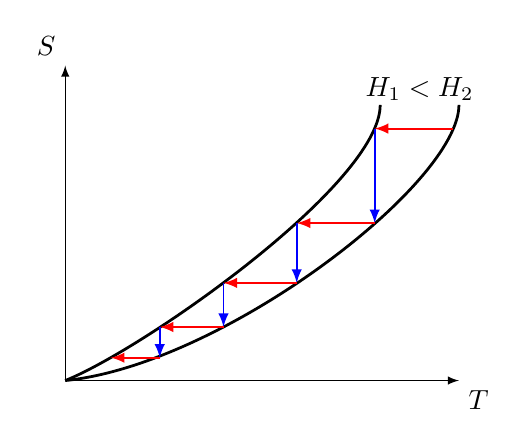
\begin{tikzpicture}
       \draw[-latex] (0,0) -- (5,0) node[below right] {$T$};
       \draw[-latex] (0,0) -- (0,4) node[above left] {$S$};
       \draw[line width=1pt] (0,0) .. controls (1,0.4) and (4,2.5) .. (4,3.5);
       \draw[line width=1pt] (0,0) .. controls (2,0.2) and (5,2.5) .. (5,3.5);
       \draw[-latex,line width=0.7pt,red] (4.92,3.2) -- (3.93,3.2);
       \draw[-latex,line width=0.7pt,blue] (3.93,3.2) -- (3.93,2);
       \draw[-latex,line width=0.7pt,red] (3.93,2) -- (2.94,2);
       \draw[-latex,line width=0.7pt,blue] (2.94,2) -- (2.94,1.24);
       \draw[-latex,line width=0.7pt,red] (2.94,1.24) -- (2.01,1.24);
       \draw[-latex,line width=0.7pt,blue] (2.01,1.24) -- (2.01,0.68);
       \draw[-latex,line width=0.7pt,red] (2.01,0.68) -- (1.2,0.68);
       \draw[-latex,line width=0.7pt,blue] (1.2,0.68) -- (1.2,0.29);
       \draw[-latex,line width=0.7pt,red] (1.2,0.29) -- (0.58,0.29);
       \node at (4.5,3.7) {$H_1 < H_2$};
       \end{tikzpicture}
       \caption{Az adiabatikus lemágnesezés folyamata.
   A piros lépésekben történik az adiabatikus lemágnesezés, a kék lépésekben pedig az izotermikus mágnesezés.}\label{fig:B03-adiablemag}
     \end{figure}
   \end{enumerate}
   

  \chapter{Sokas\'agok, eloszl\'asok, potenci\'alok}
 
 \section{Mikrokanonikus sokaság}
  
  Lásd \aref{ss:B03-mikrokansok}. fejezetet.
  
 \section{Kanonikus sokaság ($T$,$V$,$N$)}
  
  Kanonikus sokaságban egy zárt rendszer kis alrendszerét tekintjük.
   Az egész rendszer energiája rögzített ($E_0=E+E_\text{K}$), ahol $E$ az alrendszer energiája, míg $E_\text{K}$ a környezeté.
   Mivel a környezet jóval nagyobb, mint az alrendszer, ezért $E\approx E_\text{K}=\text{áll}$. 
  
  \subsection{A kanonikus eloszlás}
   
   Az eloszlás meghatározásához kiszámoljuk annak a valószínűségét, hogy az alrendszer az $i$-edik mikroállapotban van.
   Ez a szám azzal lesz egyenlő ahányféleképpen a környezet energiája $E_0-E_i$ lehet:
   \al{
    \rho(i)
     =\frac{\Omega_\text{K}(E_0-E_i,\delta E)}{\Omega_0(E_0,\delta E)}.
   }
   Mivel $E_i$ kicsi, így ezt sorbafejthetjük (a logaritmusát):
   \al{
    \ln\rho(i)
     &=\underbrace{\ln\frac{\Omega_\text{K}(E_0,\delta E)}{\Omega_0(E_0,\delta E)}}_{\text{const.}}-\pder{\ln\Omega_\text{K}(E_0,\delta E)}{E}\cdot E_i+\mathcal{O}(E_i^2)\\
     &=\underbrace{\ln\frac{\Omega_\text{K}(E_0,\delta E)}{\Omega_0(E_0,\delta E)}}_{\text{const.}}-\underbrace{\pder{\ln\Omega_\text{K}(E_\text{K},\delta E)}{E}}_{=\frac{1}{\kB T_\text{K}}}\cdot E_i+\mathcal{O}(E_i^2)
      \approx\text{const.}-\beta_\text{K}E_i.
   }
   Igy $\rho(i)\sim e^{-\beta_\text{K} E_i}$.
   A normálással együtt klasszikus és kvantumos rendszerre:
   \al{
    &\text{Klasszikus rendszerre:}
    &\rho(q,p)&=\frac{1}{Z}e^{-\beta E(q,p)}
    &Z&=\intl{}{}\frac{\dd q^{dN}\dd p^{dN}}{h^{dN}N!}\,e^{-\beta E(q,p)}\\
    &\text{Kvantumos rendszerre:}
    &\op\rho&=\frac{1}{Z}e^{-\beta \opH}
    &Z&=\tr\left(e^{-\beta \opH}\right),
   }
   ahol megelőlegeztük, hogy a környezet és a rendszer hőmérséklete egyenlő.
   Ehhez vizsgáljuk meg, hogy mekkora annak a valószínűségi sűrűsége, hogy az általunk vizsgált alrendszer energiája $E$.
   Ez abból adódik, hogy a rendszer mekkora valószínűséggel van az $i$-edik mikroállapotban, illetve hogy az állapotok milyen sűrűn vannak ($\omega(E)$ az energia-állapotsűrűség): 
   \al{
    P(E)=\rho(E)\omega(E)=\frac{e^{-\beta_\text{K}E}\omega(E)}{Z}.
   }
   Ez egy éles eloszlás, hiszen a számláló első tagja az energia növelésével élesen levág, míg $\omega(E)$ az energia növelésével élesen nő.
   Az éles eloszlás miatt a várható érték és a legvalószínűbb érték itt is jó közelítéssel megegyezik.
   Az eloszlás (logaritmusának) maximuma:
   \al{
    \ln P(E)&=-\beta_\text{K}E+\ln\omega(E)+\text{const.}\\
    0&=\pder{\ln P(E)}{E}=-\beta_\text{K}+\underbrace{\pder{\ln \omega(E)}{E}}_{\frac{1}{\kB T}}
    &\Rightarrow
    &&T=T_\text{K}.
   }
  
  \subsection{Energia várható értéke, fluktuációi}
   
   Az energia várható értéke:
   \al{
    \mv{E}
     &=\suml{i}{}E_i\rho(i)
      =\suml{i}{}\frac{E_i e^{-\beta E_i}}{\suml{j}{}e^{-\beta E_j}}
      =-\pder{\ln Z}{\beta},
   }
   illetve szórásnégyzete:
   \al{
    \mv{(\Delta E)^2}
     &=\mv{E^2}-\mv{E}^2
      =\frac{1}{Z}\pder{^2 Z}{\beta^2}-\left(\frac{1}{Z}\pder{Z}{\beta}\right)^2
      =\pder{}{\beta}\left(\frac{1}{Z}\pder{Z}{\beta}\right)
      =\pder{}{\beta}\left(\pder{\ln Z}{\beta}\right)\\
     &=-\pder{E}{\beta}
      =-\kB\underbrace{\pder{E}{T}}_{C_V}\underbrace{\pder{T}{\frac{1}{T}}}_{-T^2}
      =\kB T^2 C_V.
   }
   Az energia szórásnégyzete egy statisztikus fizikai mennyiség, míg a jobb oldalon állók termodinamikai mennyiségek.
   Mivel feltételeztük, hogy normál rendszerben vagyunk, így $C_V>0$ adódik.
   A termodinamikában ez stabilitási feltétel.
   
  \subsection{Szabadenergia}
   
   A termodinamikában az energiából Legendre-transzformációval előállítjuk a szabadenergiát: $F=E-TS$.
   A statisztikus fizikában:
   \al{
    F=-\kB T\ln Z,
   }
   ahol $Z$ az állapotszám.
   Mivel az eloszlás nagyon éles, ezért az állapotösszeg közelíthető:
   \aln{
    Z=\intl{E_\text{min}}{\infty}\dd E\,e^{-\beta E}\omega(E)
     =e^{-\beta E} \omega(E)\cdot \Delta E,\label{eq:B04-kanallszam}
   }
   ahol $\Delta E$ az eloszlás szélessége.
   A szórásnégyzetből adódik, hogy $\Delta E\sim C_V\sim N$. Így tehát
   \al{
    F=-\kB T\ln Z
     =-\kB T \big(\underbrace{-\beta E}_{\mathcal{O}(N)} +\underbrace{\ln\omega(E)}_{\mathcal{O}(N)}+ \underbrace{\ln\Delta E}_{\mathcal{O}(\ln N)}\big)
     \approx -\kB T (-\beta E + \ln\omega(E))
     =E-TS,
   }
   vagyis makroszkopikusan megegyezik a termodinamikai definícióval.
   A termodinamikai deriváltaknak megfelelő összefüggéseket is megkapjuk:
   \al{
    \pder{F}{T}
     &=\pder{}{T}(-\kB T \ln Z)
      =-\kB\ln Z-\kB T\pder{\ln Z}{T}
      =\frac{F}{T}+\frac{1}{T}\pder{\ln Z}{\beta}
      =\frac{F}{T}-\frac{E}{T}
      =-S\\
    \pder{F}{V}
     &=\pder{}{V}(-\kB T \ln Z)
      =-\kB T \pder{\ln Z}{V}
      =-\kB T \frac{1}{Z}\suml{i}{}\beta\left(-\pder{E_i}{V}\right)e^{-\beta E_i}
      =\frac{1}{Z}\suml{i}{}\pder{E_i}{V}e^{-\beta E_i}\\
     &=\mv{\pder{E}{V}}=-p
   }
   
   $F$ extenzív mennyiség, hiszen független alrendszerek összességére $Z$ szorzódik.
   Az információs entrópiába helyettesítve a kanonikus eloszlás az $S$ entrópiát adja:
   \al{
    \kB S_\text{inf}
     &=-\kB\suml{}{}\rho(i)\ln\rho(i)
      =-\kB\frac{1}{Z}\suml{}{}e^{-\beta E_i}\ln\left(\frac{1}{Z}e^{-\beta E_i}\right)\\
     &=-\kB\frac{1}{Z}\suml{}{}e^{-\beta E_i}\left(-\beta E_i-\ln Z \right)
      =\kB\beta\underbrace{\frac{1}{Z}\suml{}{} E_i e^{-\beta E_i}}_{E}
       +\kB\ln Z\underbrace{\frac{1}{Z}\suml{}{}e^{-\beta E_i}}_{1}\\
     &=\frac{E}{T}-\frac{F}{T}
      =S.
   }
   Az információs entrópiát a mikrokanonikus eloszlás maximalizálta.
   A kanonikus eloszlás az információs entrópiát az a mellékfeltétel mellett maximalizálja, hogy $E$ állandó.
   Ezt onnan tudjuk, hogy $T$-t rögzíti a környezet, és $T$ az átlagenergia, így fix részecskeszám mellett $E=\suml{}{}E_i\rho(i)=\text{const.}$ A variálás:
   \al{
    0&=\delta\left(-\suml{i}{}\rho(i)\ln\rho(i)-\lambda\suml{i}{}E_i\rho(i)\right)
      =-\suml{i}{}\left(\delta\rho(i)\ln\rho(i)+\rho(i)\frac{1}{\rho(i)}\delta\rho(i)\right)-\lambda\suml{i}{}E_i\delta\rho(i)\\
     &=\suml{i}{}\delta\rho(i)\big(-\ln\rho(i)-1-\lambda E_i\big)\\
    0&=-\ln\rho(i)-1-\lambda E_i\\
    \rho(i)&=C e^{-\lambda E_i},
   }
   ahol $C=Z$ és $\lambda=\beta$. 
   
  \section{Nagykanonikus sokaság ($T$,$V$,$\mu$)}
   
   A konstrukció hasonló az előzőhöz: most is egy elszigetelt nagy rendszer pici alrendszerét vizsgáljuk.
   Az alrendszer és a környezet között anyagi kölcsönhatás és energiatranszfer történhet, de mechanikai munka nincs ($\delta V=0$). 
   
   Bevezetjük a nagykanonikus potenciált:
   \al{
    \Phi(T,V,N)&=E-TS-\mu N=-pV
    &\dd\Phi=-S\dd T-p\dd V-N\dd\mu
   }
   A termodinamikai deriváltak:
   \al{
    &\left(\pder{\Phi}{T}\right)_{V,\mu}=-S
    &&\left(\pder{\Phi}{V}\right)_{T,\mu}=-p
    &&\left(\pder{\Phi}{\mu}\right)_{T,V}=-N.
   }
   Ebben az esetben egy mikroállapot valószínűsége: $\rho(N,i_N)$.
   A mikroállapotok valószínűsége attól is függ, hogy hány részecske van épp a rendszerben.
   Ez felírva a környezet és a teljes rendszer állapotszámaival:
   \al{
    \rho(N,i_N)=\frac{\Omega_{0,\text{K}}(E_0-E,N_0-N)}{\Omega_0(E_0,N_0)}.
   }
   Itt is sorfejtést alkalmazunk a kis $E$ és $N$-re:
   \al{
    \ln\rho(N,i_N)=\text{const}-\pder{\ln\Omega_\text{K}(E_0,N_0)}{E}E_i-\pder{\ln\Omega_\text{K}(E_0,N_0)}{N}N,
   }
   ahonnan exponencializálva és elnevezve az együtthatókat:
   \al{
    &\rho(N,i_N)=\frac{1}{\mathcal{Z}}e^{-\beta_\text{K}(E_i-\mu_\text{K} N)}
    &\mathcal{Z}=\mathcal{Z}(T,V,\mu)=\suml{N=0}{\infty}\suml{i_N}{}e^{-\beta_\text{K}(E_i-\mu_\text{K} N)}
   }
   Itt is a környezet kémiai potenciálja és redukált hőmérséklete szerepel.
   A kanonikus esethez hasonlóan itt is be lehet látni, hogy a $\beta_\text{K}=\beta$ és $\mu_\text{K}=\mu$.
   
   A nagykanonikus potenciál statisztikus fizikai definíciója:
   \al{
    \Phi=-\kB T\ln\mathcal{Z},
   }
   melyről be lehet látni, hogy az megegyezik a termodinamikai definícióval:
   \al{
    \Phi
     &=-\kB T\ln\mathcal{Z}
      =-\kB T\ln\left(\suml{i}{}e^{-\beta(E_i-\mu N)}\right)
      =-\kB T\ln\left(\suml{N=0}{\infty}e^{\beta\mu N} Z_n\right),
   }
   ahol $Z_N$ a kanonikus állapotszám $N$ részecskére.
   Használva \eqaref{eq:B04-kanallszam} egyenletet, illetve hogy az eloszlás $N$ szerint is éles
   \al{
    \Phi
     &=-\kB T\ln\left(\suml{N=0}{\infty}e^{\beta\mu N} e^{-\beta E} \omega(E)\cdot \Delta E\right)
      =-\kB T\ln\left(e^{\beta\mu N} e^{-\beta E} \omega(E)\cdot \Delta E\Delta N\right)\\
     &=-\kB T\left(\beta\mu N -\beta E +\ln\omega(E)+\ln\Delta E+\ln\Delta N\right)
      \approx -\mu N + E -\kB T\ln\omega(E)\\
     &=E-TS-\mu N.
   }
   
 \section{TPN sokaság ($T$,$p$,$N$)}
  
  Tekintsünk egy olyan alrendszer, amely mechanikai kapcsolatban van a környezettel és hőátadás is lehetséges.
   Ennek a termodinamikai potenciálja a szabadentalpia:
  \al{
   &G(T,p,N)=E-TS+pV=\mu N
   &\dd G=-S\dd T+V\dd p+\mu\dd N.
  }
  
  A mikroállapotok valószínűsége:
  \al{
   &\rho(V,i_V)=\frac{1}{Y}e^{-\beta(E_{i_V}+pV)}
   &Y=Y(T,p,N)=\intl{V}{}\drh\suml{i_V}{}e^{-\beta(E_{i_V}+pV)}.
  }
  
  A statisztikus fizikai potenciál definíciója:
  \al{
   G=-\kB T\ln Y,
  }
  amiről szintén meg lehet mutatni, hogy a termodinamikai határesetben megegyezik a szabadentalpiával.
   A termodinamikai deriváltak:
  \al{
   \pder{G}{T}
    &=-\kB\ln Y-\kB T\pder{\ln Y}{T}
     =\frac{G}{T}+\frac{1}{T}\pder{\ln Y}{\beta}
     =\frac{G}{T}-\frac{E+pV}{T}
     =-S\\
   \pder{G}{p}
    &=-\kB T\pder{\ln Y}{p}
     =\kB T\beta V
     =V\\
   \mv{(\Delta E)^2}
    &=\mv{E^2}-\mv{E}^2
     =\frac{1}{Y}\pder{^2 Y}{\beta^2}-\left(\frac{1}{Y}\pder{Y}{\beta}\right)^2
     =\pder{}{\beta}\left(\frac{1}{Y}\pder{Y}{\beta}\right)
     =\pder{}{\beta}\left(\pder{\ln Y}{\beta}\right)\\
    &=-\pder{E}{\beta}
     =\kB T^2\pder{E}{T}
     =\kB T^2 C_V\\
   \mv{(\Delta V)^2}
    &=\mv{V^2}-\mv{V}^2
     =\frac{1}{Y}\frac{1}{\beta^2}\pder{^2 Y}{p^2}-\left(-\frac{1}{Y}\frac{1}{\beta}\pder{Y}{p}\right)^2
     =\frac{1}{\beta^2}\pder{}{p}\left(\frac{1}{Y}\pder{Y}{p}\right) 
     =\frac{1}{\beta^2}\pder{}{p}\left(\pder{\ln Y}{p}\right) \\
    &=-\kB T\pder{V}{p}
     =\kB T V \kappa_T.
  }

  \chapter{Fluktu\'aci\'ok, stabilit\'as, helyf\"ugg\H{o} korrel\'aci\'o, szuszceptibilit\'as, line\'aris v\'alasz}
 
 \section{Egyensúlyi feltételek}
  
  \subsection{Mikrokanonikus sokaságon}
   
   Legyen $X$ egy extenzív mennyiség, melynek értéke $x$. $S(x)$ a feltételes entrópia, rögzítjük az $X$ értékét $x$-nek, és megnézzük, hogy akkor mennyi az entrópia.
   Az állapotszámra való átírással: $S(x)=\kB\ln\Omega(E,x)$.
   Annak a valószínűsége, hogy az extenzív mennyiség értéke $x$:
   \al{
    P(X=x)
     =\frac{\Omega(E,x)}{\suml{X}{}\Omega(E,x)}
     =\frac{\Omega(E,x)}{\Omega(E)}
     =\frac{e^{\frac{1}{\kB} S(x)}}{e^{\frac{1}{\kB} S(x_\text{eq})}}
     =e^{\frac{1}{\kB} \big(S(x)-S(x_\text{eq})\big)},
   }
   ahol felhasználtuk, hogy a makroszkopikus rendszerekben az átlagos $x_\text{eq}$ érték megegyezik a legvalószínűbbel.
   Ez alapján azt látjuk, hogy olyan $x$ értékek valósulnak meg, amelyek $S$-et maximalizálják.
   Ha $X$ nem az egyensúlyi $x$ értéket veszi fel, akkor annak a valószínűsége exponenciálisan kicsi ($S(x)-S(x_\text{eq}<0)$).
   Mivel $S\sim N$, így $\Delta S\sim N$, $P(X=x)\sim e^{-N}$, azaz $T\sim e^{N}$ idő alatt látunk csak makroszkopikus eltérést a legvalószínűbb értéktől.
   
  \subsection{Kanonikus sokaságban}
   
   Hasonlóan gondolkodunk itt is.
   Legyen az $X$ extenzív mennyiség értéke $x$.
   Kérdés, hogy ennek mekkora a valószínűsége.
   \al{
    P(X=x)
    &=\suml{\substack{i\\X=x}}{}\frac{1}{Z}e^{-\beta E_i}
     =\frac{1}{Z}\intl{}{}\dd E\,\omega(E,x) e^{-\beta E_i}
     =\frac{1}{Z}\omega(E_\text{eq},x) e^{-\beta E_\text{eq}}\Delta E\\
    &=\frac{1}{Z}e^{\frac{1}{\kB} \big(S(x)+\ln\Delta E\big)} e^{-\beta E_\text{eq}}
     \approx\frac{1}{Z}e^{\frac{1}{\kB} S(x)} e^{-\beta E_\text{eq}}
     =\frac{1}{Z}e^{-\beta\big(E_\text{eq}-T S(x)\big)}
     =\frac{1}{Z}e^{-\beta F(x)}\\
    &=\frac{e^{-\beta F(x)}}{e^{-\beta F(x_\text{eq})}}
     =e^{-\beta \big(F(x)-F(x_\text{eq})\big)}.
   }
   
   Tehát itt is látszik, hogy a legvalószínűbb $X$ érték minimalizálja $F$-et, és mivel éles az eloszlás, ezért a legvalószínűbb érték az $x$ várható értékével egyenlő.
   
  \subsection{Nagykanonikus sokaságra}
   
   Ugyanezt kell felírni, és adódik, hogy $P(X=x)=e^{-\beta\big(\Phi(x)-\Phi(x_\text{eq})\big)}$, és $x_\text{eq}$ minimalizálja $\Phi$-t. 
   
  \subsection{TPN sokaságra}
  
   Szintén $P(X=x)=e^{-\beta\big(G(x)-G(x_\text{eq})\big)}$, és $x_\text{eq}$ minimalizálja $G$-t. 
  
 \section{Einstein-módszer a fluktuációk számítására} 
  
  Az extenzív mennyiségek fluktuációja és a termodinamikai második deriváltakra vonatkozó stabilitási kritériumok között van valamilyen kapcsolat.
   Ezt általánosan az Einsteint-módszerrel lehet megadni. 
  
  Egy mikrokanonikus sokaságban legyenek $\Xv=X_1,X_2,\dots,X_n$ azok az extenzív mennyiségek, amelyeket mint feltételeket írjuk az entrópia kifejezésébe.
   Ezek az értékek az egyensúlyi értéküktől ($\Xv_\text{eq}=X_{1,\text{eq}},X_{2,\text{eq}},\dots,X_{n,\text{eq}},$) csak nagyon kicsit térnek el ($\delta X_i=X_i-X_{i,\text{eq}}$).
   Fejtsük sorba az entrópiát:
  \al{
   S(E,\Xv)
    &=S(E,\Xv_\text{eq})+\frac{1}{2}\suml{i,j}{}\underbrace{\left.\pder{^2 S}{X_i\partial X_j}\right|_{\Xv_\text{eq}}}_{-g_{ij}}\delta X_i\delta X_j+\dots,
  }
  ahol bevezettük a $g_{ij}$ mátrixot, ami pozitív definit, hiszen $S$ maximuma körül végezzük a sorfejtést.
   Ezzel megadhatjuk, hogy mekkora annak a valószínűsége, hogy az $\Xv$ állapot valósul meg:
  \al{
   P(\Xv)
    &=\frac{\Omega(E,\Xv)}{\Omega(E)}
     \sim e^{-\frac{1}{2\kB}\suml{i,j}{}g_{ij}\delta X_i\delta X_j}\\
    &=\sqrt{\frac{\det{g}}{(2\pi\kB)^n}}e^{-\frac{1}{2\kB}\suml{i,j}{}g_{ij}\delta X_i\delta X_j},
  }
  ahol a normálási faktor abból jött, hogy $X_i$-k szerint integrálva Gauss-integrálokat kapunk, és annak ismerjük az értékét. 
  
  Vezessük be az $X_i$ extenzív mennyiségekhez tartozó konjugált tereket $h_i$, és írjuk fel az alábbi integrált:
  \al{
   f(\Xv,\hv)
    =\sqrt{\frac{\abs{\det{g}}}{(2\pi\kB)^n}}\intl{}{}\dd X_1\dots \dd X_n\,e^{-\frac{1}{2\kB}\suml{i,j}{}g_{ij}\delta X_i\delta X_j-\suml{i}{} h_i \delta X_i},
  }
  ahonnan 
  \al{
   \mv{\delta X_i\delta X_j}
    =\lim_{\hv\to 0}\pder{^2 f}{h_i\partial h_j}=\kB [g^{-1}]_{ij}.
  }
  
  \subsection{Példa: állandó anyagmennyiség}
   
   A feltételes entrópiát írjuk fel úgy, hogy $\Xv=(E,V)$, vagyis a rendszer energiáját és térfogatát adjuk meg mi előre.
   Ekkor az $S$ sorfejtése:
   \al{
    S(E,V)
     &=S(E_\text{eq},V_\text{eq})
     +\frac{1}{2}
       \left(
        \left.\pder{^2 S}{E^2}\right|_{\text{eq}}\delta E^2
       +2\left.\pder{^2 S}{E\partial V}\right|_{\text{eq}}\delta E\delta V
       +\left.\pder{^2 S}{V^2}\right|_{\text{eq}}\delta V^2
       \right)
   }
   Használjuk fel, hogy 
   \al{
    \delta\left(\pder{S}{V}\right)
     &=\pder{^2 S}{V^2}\delta V+\pder{^2 S}{E\partial V}\delta E
    &\delta\left(\pder{S}{E}\right)
     &=\pder{^2 S}{E^2}\delta E+\pder{^2 S}{V\partial E}\delta V,
   }
   így
   \al{
    S(E,V)-S(E_\text{eq},V_\text{eq})
     &=\frac{1}{2}\left(\delta V\delta\left(\pder{S}{V}\right)+\delta E\delta\left(\pder{S}{E}\right)\right)
      =\frac{1}{2}\left(\delta V\delta \frac{p}{T}+\delta E\delta\frac{1}{T}\right)\\
     &=\frac{1}{2}\left(\delta V \frac{1}{T}\delta p-\delta V \frac{1}{T^2}p\delta T-\delta E\frac{1}{T^2}\delta T\right)\\
     &=\frac{1}{2T}\left(\delta V \delta p-\frac{\delta T}{T}(\delta E+p\delta V)\right)\\
     &=\frac{1}{2T}\left(\delta V \delta p-\delta T\delta S\right)
   }
   Fejtsük ki $\delta S$-t és $\delta p$-t:
   \al{
    \delta S
     &=\left(\pder{S}{T}\right)_V\delta T+\left(\pder{S}{V}\right)_T\delta V
      =\frac{1}{T}C_V\delta T +\left(\pder{p}{T}\right)_V\delta V\\
    \delta p
    &=\left(\pder{p}{T}\right)_V\delta T+\left(\pder{p}{V}\right)_T\delta V
     =\left(\pder{p}{T}\right)_V\delta T-(V\kappa_T)^{-1}\delta V.
   }
   Az első átalakításánál használtuk az egyik Maxwell-összefüggést.
   Ezeket behelyettesítve:
   \al{
    S(E,V)-S(E_\text{eq},V_\text{eq})
     &=\frac{1}{2T}\left(\left(\pder{p}{T}\right)_V \delta V\delta T-(V\kappa_T)^{-1}\delta V^2-\frac{1}{T}C_V\delta T^2 -\left(\pder{p}{T}\right)_V\delta T\delta V\right)\\
     &=-\frac{1}{2T}\left((V\kappa_T)^{-1}\delta V^2+\frac{1}{T}C_V\delta T^2\right),
   } 
   ahonnan valószínűség:
   \al{
    P(E,V)
     =e^{\frac{1}{\kB}\big(S(E,V)-S(E_\text{eq},V_\text{eq})\big)}
     =e^{-\frac{1}{2 \kB T}\left((V\kappa_T)^{-1}\delta V^2+\frac{1}{T}C_V\delta T^2\right)}.
   }
   Innen le tudjuk olvasni, hogy 
   \al{
    &\mv{(\delta V)^2}
     =\frac{\kB T}{(V\kappa_T)^{-1}}
      =\kB T V\kappa_T
    &\mv{(\delta T)^2}
     =\frac{\kB T^2}{C_V}
    &&\mv{\delta V\delta T}
     =0.
   }
   
  \subsection{Példa: sűrűségfluktuációk}
   
   Legyen elször $N$ fix.
   Ekkor
   \al{
    \mv{(\delta n)^2}
     &=\mv{\left(\delta \frac{N}{V}\right)^2}
      =\mv{\left(-\frac{N}{V^2}\delta V\right)^2}
      =\frac{N^2}{V^4}\mv{(\delta V)^2}
      =\frac{N^2}{V^4}\kB T V\kappa_T
      =\frac{n^2}{V}\kB T \kappa_T.
   }
   Ha $V$ fix, akkor 
   \al{
    \mv{(\delta n)^2}
     &=\mv{\left(\delta \frac{N}{V}\right)^2}
      =\frac{1}{V^2}\mv{(\delta N)^2}
     &\Rightarrow
     &&\mv{(\delta N)^2}=\kB T n^2 V\kappa_T.
   }
   
 \section{Lineáris válasz}\label{ss:B05-linvalasz}
  
  Nézzük meg, hogy milyen a rendszer válasza egy klasszikus $F$ külső erőre.
   Tegyük fel, hogy kezdetben a rendszer Hamilton-függvénye $H_0$, majd a klasszikus erő az $Y$ extenzív mennyiséghez csatolódik:
  \al{
   H=H_0-Y F.
  }
  Kanonikus sokasággal leírva a rendszerben az $X$ várhatóértékében beállt változást számoljuk ki:
  \al{
   \mv{X(F)}
    &=\frac{\suml{q,p}{}\left(X e^{-\beta\big(H_0-Y F\big)}\right)}{\suml{q,p}{}\left( e^{-\beta\big(H_0-Y F\big)}\right)}&
   \mv{X(F=0)}
    &=\frac{\suml{q,p}{}\left(X e^{-\beta H_0}\right)}{\suml{q,p}{}\left( e^{-\beta H_0}\right)}.
  }
  Mivel $F$ kicsi valamilyen értelemben ($YF\ll H_0$), ezért $X$ megváltozása kicsi, arányos $F$-fel: $\mv{X(F)}-\mv{X(F=0)}\approx\chi_{XY} F$, ahol $\chi_{XY}$ az általánosított szuszceptibilitás. 
  \al{
   \chi_{XY}
    &=\lim_{F\to 0}\frac{\mv{X(F)}-\mv{X(F=0)}}{F}
     =\pder{\mv{X}}{F}
     =\left.\pder{}{F}\right|_{F=0}\frac{\suml{q,p}{}\left(X e^{-\beta\big(H_0-Y F\big)}\right)}{\suml{q,p}{}\left( e^{-\beta\big(H_0-Y F\big)}\right)}\\
    &=
      \left(
       \beta\frac{\suml{q,p}{}\left(XY e^{-\beta\big(H_0-Y F\big)}\right)}{\suml{q,p}{}\left( e^{-\beta\big(H_0-Y F\big)}\right)}
       -\frac{\suml{q,p}{}\left(X e^{-\beta\big(H_0-Y F\big)}\right)}{\left[\suml{q,p}{}\left( e^{-\beta\big(H_0-Y F\big)}\right)\right]^2}\beta\suml{q,p}{}\left(Y e^{-\beta\big(H_0-Y F\big)}\right)
      \right)_{F=0}\\
    &=
      \left(
       \beta\mv{XY}_{\opH}
       -\beta\mv{X}_{\opH}\mv{Y}_{\opH}\right)_{F=0}
     =\beta\mv{XY}_{\opH_0}-\beta\mv{X}_{\opH_0}\mv{Y}_{\opH_0}
     =\beta\mv{(\delta X)(\delta Y)}_{\opH_0}.
  }
  Tehát a rendszer válasza kizárólag a perturbálatlan rendszertől függ.

 \section{Helyfüggés, korrelációk}
  
  Legyen az $X$ és $Y$ egy-egy extenzív mennyiség.
   Ezeknek sűrűsége helyfüggő: $x(\rv)$ és $y(\rv)$, mellyel $X=\intl{}{}\drh x(\rv)$ és $x_\text{eq}=\frac{X_\text{eq}}{V}$.
   Az $Y$-ra teljesen hasonló összefüggések írhatóak fel.
   A korrelációs függvény:
  \al{
   C_{XY}(\rv,\rv')=\mv{\big(x(\rv)-x_\text{eq}\big)\big(y(\rv')-y_\text{eq}\big)}.
  }
  Transzlációinvariáns rendszerben $C_{XY}(\rv,\rv')=C_{XY}(\rv-\rv')$.
   Ennek kapcsolata a fluktuációkkal:
  \al{
    \intl{}{}\drh\intl{}{}\drkh C_{XY}(\rv,\rv')=
    &=\intl{}{}\drh\intl{}{}\drkh \mv{\big(x(\rv)-x_\text{eq}\big)\big(y(\rv')-y_\text{eq}\big)}\\
    &=\mv{\intl{}{}\drh\big(x(\rv)-x_\text{eq}\big)\intl{}{}\drkh \big(y(\rv')-y_\text{eq}\big)}\\
    &=\mv{\big(X-X_\text{eq}\big)\big(Y-Y_\text{eq}\big)}
     =\mv{(\delta X)(\delta Y)}.
  }
  
  Fontos kapcsolat álla fenn a korrelációs függvények és a lineáris válasz között.
   Az előző két eredményt összevetve:
  \al{
   \chi_{XY}=\beta \intl{}{}\drh\intl{}{}\drkh C_{XY}(\rv,\rv').
  }
  Például a mágnesezettségi sűrűségre ez felírva:
  \al{
   \chi
    =\beta\mv{(\delta M)^2}_{H=0}
    =\beta\intl{}{}\drh\intl{}{}\drkh C_{mm}(\rv,\rv').
  }  

  \chapter{Klasszikus g\'azok: ide\'alis g\'az, ekvipart\'{\i}ci\'o, Maxwell-eloszl\'as, viri\'al sorfejt\'es, van der Waals \'allapotegyenlet} 
 
 \section{Ekvipartíció tétele}
  
  Tekintsünk egy klasszikus rendszert.
   Ennek Hamilton-függvénye $H=H(q,p)$.
   Jelölje $x_i$ a Hamilton-függvény tetszőleges változóját, $q_i$-t vagy akár $p_i$-t is.
   Az $x_i$-t szabadsági foknak hívjuk, ha 
  \al{
   \lim_{x_i\to \pm\infty}H(\dots,x_i,\dots)=\infty.
  }
  Fontos, hogy mind a két határértékben divergálnia kell a Hamilton-függvénynek.
   Az ekvipartíció tétele kimondja, hogy ha $x_i$ szabadsági fok, akkor 
  \al{
   \mv{x_j\pder{H}{x_i}}=\delta_{ij}\kB T.
  }
  Bizonyítás:
  \al{
   \mv{x_j\pder{H}{x_i}}
    &=\frac{1}{Z}\intl{}{}\frac{\dd^{dN}p\dd^{dN}q}{N! h^{dN}}\,e^{-\beta H}x_j\pder{H}{x_i},
  }
  ahol végezzük el külön az $x_i$-re való integráli:
  \al{
   \intl{}{}\dd x_i\,e^{-\beta H}x_j\pder{H}{x_i}
    &=-\frac{1}{\beta}\intl{}{}\dd x_i\,x_j\pder{e^{-\beta H}}{x_i}
     =\{\text{parc. int.}\}\\
    &=-\frac{1}{\beta}\left(\left[x_j e^{-\beta H}\right]_{x_i=-\infty}^{x_i=\infty}-\intl{}{}\dd x_i\,\pder{x_j}{x_i}e^{-\beta H}\right)
     =\frac{1}{\beta}\intl{}{}\dd x_i\,\underbrace{\pder{x_j}{x_i}}_{\delta_{ij}} e^{-\beta H},
  } 
  így
  \al{
   \mv{x_j\pder{H}{x_i}}
    &=\frac{1}{Z}\frac{1}{N! h^{dN}}\intl{}{}\dd^{dN}p\dd^{dN}q\,\frac{1}{\beta}\pder{x_j}{x_i}e^{-\beta H}
     =\frac{1}{\beta}\delta_{ij}\frac{1}{Z}\underbrace{\frac{1}{N! h^{dN}}\intl{}{}\dd^{dN}p\dd^{dN}q\,e^{-\beta H}}_{=Z}
     =\kB T\delta_{ij}.
  }
  
  Még egyszer, ez csak klasszikus rendszerekben igaz.
   Alacsony hőmérsékleten nem ugyanakkora energia jut az egyes szabadsági fokokra, vannak szabadsági fokok, amelyek kifagynak.
   Pl. a Doulong--Petit-törvény szerint a harmonikus oszcillátor fajhője állandó, míg a kvantumos levezetésből alacsony hőmérsékleten $\sim T^2$ adódik. 
  
 \section{Klasszikus ideális gáz}\label{ss:B06-CID}
  
  Ideális klasszikus gáznak tekintjük azt a rendszert, amely
  \begin{itemize}
   \item klasszikus (nem kvantumos) fizikával leírható,
   \item a részecskék pontszerűnek tekinthetőek (térfogatuk elhanyagolható),
   \item a falakkal tökéletesen rugalmasan ütköznek a részecskék (energia megmarad),
   \item a részecskék közötti kölcsönhatást csak olyan értelemben vesszük figyelembe, hogy a rendszer termalizálódik, egyéb effektusokkal nem számolunk.
  \end{itemize}
  
  \subsection{Állapotszám}
  
   Legyen $N$ részecske a $d$ dimenziós, $V$ térfogatot kitöltő klasszikus ideális gázban.
   Mikrokanonikus sokaságként kezelve az állapotszám:
   \al{
    \Omega_{0}(E)
     =\intl{\suml{i=1}{N}\frac{p_i^2}{2m}<E}{}\frac{\dd^{dN}p\dd^{dN}q}{N! h^{dN}}\,
     =\frac{V^{N}}{N! h^{dN}}\underbrace{\intl{p_1^2+p_2^2+\dots<2mE}{}\,\dd^{dN}p}_{\substack{\text{$dN$ dimenziós $\sqrt{2mE}$}\\ \text{sugarú gömb térfogata}}}
     =\frac{V^{N}}{N! h^{dN}}\frac{(2mE)^{\frac{dN}{2}}\pi^{\frac{dN}{2}}}{\Gamma\left(\frac{dN}{2}+1\right)},
   }
   ahol $\Gamma$ a Gamma-függvény (a faktoriális általánosítása).
   
   Az entrópiához szükségünk van ennek a logaritmusára.
   A Stirling-formulát ($\ln n!\approx n\ln n-n$) használva, illetve a Gamma-függvényt közelítve ($\Gamma(n+1)\sim n!$): 
   \al{
    \ln{\Omega_0(E)}
     &\approx N\ln V-(N\ln N-N)-dN\ln h+\frac{dN}{2}\ln(2mE\pi)-\left(\frac{dN}{2}\ln\frac{dN}{2}-\frac{dN}{2}\right)+\mathcal{O}(\ln N)\\
     &=N\ln V-(N\ln N-N)+\frac{dN}{2}\ln\left(\frac{4mE\pi}{dNh^2}\right)+\frac{dN}{2}+\mathcal{O}(\ln N)\\
     &=\frac{2+d}{2}N+\frac{dN}{2}\ln\left(\frac{4m\pi}{dh^2}\frac{E}{N}\left(\frac{V}{N}\right)^{\frac{2}{d}}\right)+\mathcal{O}(\ln N)\\
     &=N\underbrace{\left[\frac{2+d}{2}+\frac{d}{2}\ln\left(\frac{4m\pi}{dh^2}\frac{E}{N}\left(\frac{V}{N}\right)^{\frac{2}{d}}\right)\right]}_{=\phi\left(\frac{E}{N},\frac{V}{N}\right)}+\mathcal{O}(\ln N).
   }
   Láthatjuk, hogy ez egy normál rendszer \eqaref{eq:B03-Omega--N} egyenlet alapján. 
   
  \subsection{Maxwell-féle sebességeloszlás}
   
   Írjuk le az ideális gázt kanonikus sokaságban.
   A Hamilton-függvény $H=\suml{i=1}{N}\frac{p_i^2}{2m}$.
   Mivel a Hamilton kölcsönhatásmentes, így a kanonikus állapotszám:
   \al{
    Z&=\frac{Z_1^N}{N!}\\
    Z_1&=\frac{1}{h^3}\intl{}{}\dd^3 \qv\dd^3 \pv\,e^{-\beta\frac{p^2}{2m}}
        =\frac{V}{h^3}\intl{}{}\dd^3 \pv\,e^{-\beta\frac{\pv^2}{2m}}
       =\frac{V}{h^3}\left(\frac{2m\pi}{\beta}\right)^{\frac{3}{2}}
        =\frac{V}{h^3}\left(2\pi m\kB T\right)^{\frac{3}{2}}.
   }
   Annak a valószínűsége, hogy egy részecske impulzusa $\pv$:
   \al{
    P(\pv)
     =\frac{\frac{1}{h^{3N}}\intl{}{}\dd^{3N} q\dd^{3(N-1)} p\,e^{-\beta\suml{i=1}{N}\frac{p_i^2}{2m}}}{Z}
     =\frac{\frac{V}{h^3}e^{-\beta\frac{\pv^2}{2m}}}{Z_1}
     =\frac{e^{-\beta\frac{\pv^2}{2m}}}{\left(2\pi m\kB T\right)^{\frac{3}{2}}}.
   }
   Az előző állítás nem csak kölcsönhatásmentes rendszerekre igaz, hanem olyanokra is, ahol a kölcsönhatás csak a $q$-tól függ.
   Az előző képletben a számlálóban és a nevezőben ugyanaz a térintegrál lenne, így egyszerűsíteni lehetne vele.
   
   Az impulzus eloszlásából kifejezhetjük, hogy mennyi a valószínűsége, hogy a részecske sebessége $\vv$, hiszen:
   \al{
    &P(\vv)\dd^3\vv=P(\pv)\dd^3\pv
    &\pv=m\vv
    &&P(\vv)=m^3 P(\pv)=\left(\frac{m}{2\pi \kB T}\right)^{\frac{3}{2}}e^{-\frac{m\vv^2}{2\kB T}}.
   }
   A sebesség abszolút értékének eloszlása a Maxwell-féle sebességeloszlás:
   \al{
    &\dd^3\vv=4\pi v^2\dd v
    &P(v)
     =4\pi v^2 P(\vv)
   }
   \aln{
     \boxed{P(v)=4\pi v^2\left(\frac{m}{2\pi \kB T}\right)^{\frac{3}{2}}e^{-\frac{m v^2}{2\kB T}}}.\label{eq:B06-Maxwell}
   }
   
   Az eloszlás maximumhelye:
   \al{
    P'(v)
     &=0
      =\der{}{v}\left(-\frac{m v^2}{2\kB T}+2\ln v\right)
      =-\frac{m v}{\kB T}+2\frac{1}{v}
     &v_\text{max}=\sqrt{\frac{2\kB T}{m}},
   }
   várható értéke és négyzetes közepe:
   \al{
    \mv{v}
     &=\intl{0}{\infty}\dd v\, vP(v)
      =\intl{0}{\infty}\dd v\, 4\pi v^3\left(\frac{m}{2\pi \kB T}\right)^{\frac{3}{2}}e^{-\frac{m v^2}{2\kB T}}
      =\sqrt{\frac{8\kB T}{\pi m}}\\
    \mv{v^2}
     &=\frac{2}{m}\frac{3}{2}\kB T
      =\frac{3\kB T}{m}.
   }
   Itt messze nem igaz, hogy az eloszlás éles lenne, egy részecske sebességének az eloszlása igen széles tartományban van. 
   
   Az energia szerinti eloszláshoz:
   \al{
    &\dd E=mv\dd v
    &E=\frac{1}{2}mv^2
    &&P(E)=\frac{1}{mv}P(v)
   }
   \al{
    P(E)
     &=\frac{1}{m}4\pi v\left(\frac{m}{2\pi \kB T}\right)^{\frac{3}{2}}e^{-\frac{m v^2}{2\kB T}}
      =\frac{1}{m}4\pi \sqrt{\frac{2E}{m}}\left(\frac{m}{2\pi \kB T}\right)^{\frac{3}{2}}e^{-\frac{E}{\kB T}}
      =2\pi \sqrt{E}\left(\frac{1}{\pi \kB T}\right)^{\frac{3}{2}}e^{-\frac{E}{\kB T}}.
   }
   Ennek maximumhelye és várható értéke:
   \al{
    \der{}{E}P(E)&=0
      =\der{}{E}\left(-\frac{E}{\kB T}+\frac{1}{2}\ln E\right)
      =-\frac{1}{\kB T}+\frac{1}{2E}
     & E_\text{max}=\frac{1}{2}\kB T\\
    \mv{E}&=\frac{3}{2}\kB T.
   }
   
   Az energia szórása:
   \al{
    \mv{(\Delta E)^2}
     &=\mv{E^2}-\mv{E}^2
      =\pder{}{\beta}\pder{\ln Z_1}{\beta}
      =\frac{3}{2}(\kB T)^2
      =\frac{2}{3}\mv{E}^2\\
     \frac{\sqrt{\mv{(\Delta E)^2}}}{\mv{E}}
      &=\sqrt{\frac{2}{3}}\sim\mathcal{O}(1),
   }
   ami egy részecskére igen jelentős, de az $N$ részecskéből álló gázra, ahol
   \al{
    \ln Z
     &=\ln\left(\frac{Z_1^N}{N!}\right)
      \approx -N\ln N+N+N\ln Z_1
      =-N\ln N+N+N\ln \left(\frac{V}{h^3}\left(2\pi m\kB T\right)^{\frac{3}{2}}\right)\\
    \mv{(\Delta E)^2}
     &=\pder{}{\beta}\pder{\ln Z}{\beta}
      \sim N\\
    \frac{\sqrt{\mv{(\Delta E)^2}}}{\mv{E}}&\sim\frac{1}{\sqrt{N}}.
   }
   
   Az ideális gáz állapotegyenletét megadhatjuk pl.\ az $F$ termodinamikai deriváltjával:
   \al{
    p&=-\pder{F}{V}
      =-\pder{}{V}\left(-\kB T \ln Z\right)
      =-\pder{}{V}\left(-\kB T N\ln \left(\frac{V}{N h^3}\left(2\pi m\kB T\right)^{\frac{3}{2}}\right)\right)\\
     &=\frac{1}{V}\kB T N\\
    pV&=N\kB T.
   }
   
 \section{Viriál tétel}
  
  Tegyük fel, hogy a klasszikus háromdimenziós rendszerünk Hamilton-függvénye a következő:
  \al{
   H=E_\text{kin}+U_\text{pot}=E_\text{kin}+U_\text{int}+U_\text{w},
  }
  ahol a kölcsönhatást két részre osztottuk, a részecskék egymással való kölcsönhatására és a fallal való kölcsönhatásra.
   Azt tudjuk az ekvipartíció tétele miatt, hogy $\mv{E_\text{kin}}=\frac{3}{2}\kB T$.
   Kérdés, hogy mennyi a potenciális energia átlagértéke. 
  
  A Newton-egyenletből:
  \al{
   m_i \ddot{x}_i=F_i=-\pder{U_\text{pot}}{x_i}=-\pder{H}{x_i}.
  }
  Ez beszorozva $x_i$-vel és kicsit átalakítva:
  \al{
   \der{}{t}\left(\frac{1}{2}m_ix_i\dot{x}_i\right)-\frac{1}{2}m_i\dot{x}_i^2=\underbrace{\frac{1}{2}x_i F_i}_{\text{viriál}}.
  }
  Az egyenlet időátlaga:
  \al{
   \underbrace{\lim_{\tau\to\infty}\frac{1}{\tau}\intl{0}{\tau}\dd t\,
   \der{}{t}\left(\frac{1}{2}m_ix_i\dot{x}_i\right)}_{\text{I.}}
   -\underbrace{\lim_{\tau\to\infty}\frac{1}{\tau}\intl{0}{\tau}\dd t\,\frac{1}{2}m_i\dot{x}_i^2}_{\text{II.}}
   &=\underbrace{\lim_{\tau\to\infty}\frac{1}{\tau}\intl{0}{\tau}\dd t\,\frac{1}{2}x_i F_i}_{\text{III.}}
  }
  A tagok kifejtve:
  \al{
   \text{I.}
    &=\lim_{\tau\to\infty}\frac{1}{\tau}\underbrace{\left[\frac{1}{2}m_ix_i\dot{x}_i\right]_{0}^{\tau}}_{\text{véges}}=0\\
   \text{II.}
    &=\lim_{\tau\to\infty}\frac{1}{\tau}\intl{0}{\tau}\dd t\,\frac{1}{2}m_i\dot{x}_i^2
     =\mv{E_{\text{kin},i}}\\
   \text{III.}
    &=\lim_{\tau\to\infty}\frac{1}{\tau}\intl{0}{\tau}\dd t\,\frac{1}{2}x_i F_i
     =\frac{1}{2}\mv{x_i F_i},
  }
  ahonnan a viriál tétel $i$-re való összegzéssel:
  \aln{
   \boxed{0=\mv{E_\text{kin}}+\frac{1}{2}\mv{\suml{i=1}{3N}x_i F_i}}.\label{eq:B06-virialtetel}
  }
  
  Először tekintsük csak a fallal való kölcsönhatást. 
  \al{
   U_\text{w}=\suml{i=1}{N}\ointl{\partial V}{}\dd A_\rv w(\rv_i-\rv),
  }
  ahol az integrál a fal teljes felületére megy.
   Ezzel a viriál átlagértéke:
  \al{
   \frac{1}{2}\mv{\suml{i=1}{3N}x_i F_i}
    &=-\frac{1}{2}\mv{\suml{i=1}{N}\rv_i\pder{U_\text{w}}{\rv_i}}
     =-\frac{1}{2}\mv{\suml{i=1}{N}\rv_i\ointl{\partial V}{}\dd A_\rv \grad_i w(\rv_i-\rv)}\\
    &=-\frac{1}{2}\mv{\suml{i=1}{N}\ointl{\partial V}{}\dd A_\rv \rv_i\underbrace{\grad_i w(\rv_i-\rv)}_{\text{nagyon éles}}}
     =-\frac{1}{2}\mv{\suml{i=1}{N}\ointl{\partial V}{}\dd A_\rv \rv\grad_i w(\rv_i-\rv)}\\
    &=\frac{1}{2}\mv{\suml{i=1}{N}\ointl{\partial V}{}\dd A_\rv \rv\grad_\rv w(\rv_i-\rv)}
     =\frac{1}{2}\ointl{\partial V}{}\dd A_\rv \rv\underbrace{\grad_\rv\mv{\suml{i=1}{N} w(\rv_i-\rv)}}_{\substack{\text{erő felületi sűrűsége,}\\\text{azaz a nyomás}}}\\
    &=\frac{1}{2}\ointl{\partial V}{}\dd A_\rv \rv \left(-\ev_\text{felület} p\right)
     =-\frac{p}{2}\ointl{\partial V}{}\df_\rv \rv
     =-\frac{p}{2}\intl{V}{}\drh \divo\rv
     =-\frac{3}{2}p\intl{V}{}\drh
     =-\frac{3}{2}pV.
  }
  Összefoglalva a viriál tétel:
  \al{
   \mv{E_\text{kin}}=\frac{3}{2}pV
  }
  
 \section{Viriál sorfejtés}
  
  Most vesszük figyelembe a gáz részecskéi közötti párkölcsönhatásokat:
  \al{
   U_\text{int}
    &=\suml{\mv{i,j}}{}U(\rv_i-\rv_j)
  }A viriál tétel alapján:
  \al{
   pV
    &=\frac{2}{3}\mv{E_\text{kin}}+\frac{2}{3}\frac{1}{2}\mv{\suml{i=1}{N}\rv_i\Fv_i}
     =\frac{2}{3}\mv{E_\text{kin}}-\frac{2}{3}\frac{1}{2}\mv{\suml{i=1}{N}\rv_i\suml{j(\ne i)}{}\pder{U(\rv_i-\rv_j)}{\rv_i}}\\
    &=\frac{2}{3}\mv{E_\text{kin}}-\frac{2}{3}\frac{1}{2}\frac{1}{2}\mv{\suml{i}{}\suml{j(\ne i)}{}\left(\rv_i\pder{U(\rv_i-\rv_j)}{\rv_i}+\rv_j\pder{U(\rv_i-\rv_j)}{\rv_j}\right)}\\
    &=\frac{2}{3}\mv{E_\text{kin}}-\frac{1}{6}\mv{\suml{i\ne j}{N}(\rv_i-\rv_j)\pder{U(\rv)}{\rv}}.
  }
  A jobb oldal a sorba fejthető: $p=n\kB T\big[1+b(T)n+c(T)n^2+\dots\big]$, ahol $b(T)$, $c(T)$\dots a viriál együtthatók.
  
  \subsection{Klasszikus híg gázok viriál sorfejtése}
   
   Nagykanonikus sokasággal felírva:
   \aln{
    pV=-\Phi=\kB T\ln\mathcal{Z}
     =\kB T\ln\left(\suml{N=0}{\infty}Z_Ne^{\beta\mu N}\right).\label{eq:B06-virialsf1}
   }
   Ideális gázra Láttuk, hogy 
   \al{
    &Z_1=\frac{V}{h^3}\left(2\pi m\kB T\right)^{\frac{3}{2}}
     =\frac{V}{\lambda_T^3}
    &\lambda_T=\frac{h}{\sqrt{2m\pi\kB T}},
   }
   így az állapotegyenlet
   \al{
    pV&=\kB T\ln\left(\suml{N=0}{\infty}\frac{1}{N!}(Z_1 e^{\beta\mu })^N\right)
     =\kB T Z_1 e^{\beta\mu}
     =\kB T \frac{V}{\lambda_T^3} e^{\beta\mu}
     =N\kB T,
   }
   ahonnan $e^{\beta\mu}=\lambda_T^3 n$. $\lambda_T$ értéke fix és pici, így ha $n$ kicsi, akkor $e^{\beta\mu}$ is az.
   Nem ideális gázra is azt gondoljuk, hogy ez kicsi marad, így ez a kis paraméter, ami szerint \eqaref{eq:B06-virialsf1} egyenlet jobb oldalát sorba fejtjük.
   Az állapotösszeg: $\mathcal{Z}=1+Z_1 e^{\beta\mu}+Z_2 e^{2\beta\mu}+\dots$, illetve $\ln(1+x)=x-\frac{x^2}{2}+\dots$, így
   \al{
    pV&=\kB T\ln\left(1+Z_1 e^{\beta\mu}+Z_2 e^{2\beta\mu}+\dots\right)\\
      &=\kB T\Big(Z_1 e^{\beta\mu}+Z_2 e^{2\beta\mu}+\dots-\frac{1}{2}\left(Z_1 e^{\beta\mu}+Z_2 e^{2\beta\mu}+\dots\right)^2+\dots\Big)\\
      &=\kB T\bigg(\underbrace{Z_1}_{z_1} e^{\beta\mu}+\underbrace{\left(Z_2-\frac{1}{2}Z_1^2\right)}_{z_2} e^{2\beta\mu}+\dots\bigg).
   }
   A részecskeszámot szeretnénk inkább látni az egyenlet jobb oldalán, így kifejezzük azt is
   \al{
    N=\pder{\ln\mathcal{Z}}{(\beta\mu)}
     =z_1 e^{\beta\mu}+2z_2 e^{2\beta\mu}+\dots.
   }
   Itt kicsi hibát vétünk, ha felhasználjuk az ideális gáznál kapott $e^{\mu\beta}=\frac{N}{z_1}$ összefüggést a másodrendű tagban:
   \al{
    N
     &=z_1 e^{\beta\mu}+2 z_2 \frac{N^2}{z_1^2}+\dots,
     &\Rightarrow
     &&z_1 e^{\beta\mu}\approx N-2 z_2 \frac{N^2}{z_1^2}.
   }
   Ezeket behelyettesítve a sorfejtésbe:
   \al{
    pV
     &\approx \kB T\left(z_1 e^{\mu\beta}+z_2 e^{2\mu\beta}\right)
      =\kB T\left(N-2 z_2 \frac{N^2}{z_1^2}+z_2 \frac{N^2}{z_1^2}\right)
      =\kB T\left(N-z_2 \frac{N^2}{z_1^2}\right)\\
     &=N\kB T\left(1-N\frac{Z_2-\frac{1}{2}Z_1^2}{Z_1^2}\right).
   }
   Már csak $Z_1$-et és $Z_2$-t kell kiszámolni. $Z_1$ az egyrészecskés állapotösszeg, ebben nem szerepel kölcsönhatás, így ezt ismerjük.
   A kétrészecskés állapotösszeg definíció szerint:
   \al{
    Z_2
     &=\intl{}{}\frac{\dd^3\pv_1\dd^3\pv_2\dd^3\rv_1\dd^3\rv_2}{2 h^6}\,e^{-\beta\big(\frac{\pv_1^2}{2m}+\frac{\pv_2^2}{2m}+U(\rv_1-\rv_2)\big)}
      =\frac{1}{2\lambda_T^6}\intl{}{}\dd^3\rv_1\dd^3\rv_2\,e^{-\beta U(\rv_1-\rv_2)}\\
     &=\frac{V}{2\lambda_T^6}\intl{}{}\dd^3\rv\,e^{-\beta U(\rv)}.
   }
   Mellyek a $b(T)$ viriál együttható:
   \al{
    b(T)
     &=-V\frac{Z_2-\frac{1}{2}Z_1^2}{Z_1^2}
      =-\frac{V}{2}\left(\frac{2 Z_2}{Z_1^2}-1\right)
      =-\frac{V}{2}\left(\frac{2 \lambda_T^6 Z_2}{V^2}-1\right)\\
     &=-\frac{V}{2}\left(\frac{2 \lambda_T^6}{V^2}\frac{V}{2\lambda_T^6}\intl{}{}\dd^3\rv\,e^{-\beta U(\rv)}-1\right)
      =-\frac{1}{2}\left(\intl{}{}\dd^3\rv\,e^{-\beta U(\rv)}-V\right)\\
     &=-\frac{1}{2}\intl{}{}\dd^3\rv\,\left(e^{-\beta U(\rv)}-1\right)
   }
   
   \paragraph{Példa: híg gáz, kemény mag}
    
    Legyen a kölcsönhatás ``hard ball'' potenciál:
    \al{
     U_\text{int}=\begin{cases}
                   \infty, & \text{ha }r<\sigma\\
                   0, & \text{ha }r>\sigma.
                  \end{cases}
    }
    Erre:
    \al{
     b(T)
     &=-\frac{1}{2}\intl{0}{\infty}\dd^3\rv\,\left(e^{-\beta U(\rv)}-1\right)
      =-\frac{1}{2}\intl{0}{\infty}\dd r\,4\pi r^2\left(e^{-\beta U(r)}-1\right)
      =\frac{1}{2}\intl{0}{\sigma}\dd r\,4\pi r^2
      =\frac{2\pi}{3}\sigma^3,
    }
    mellyel:
    \al{
     pV=N\kB T\left[1+\frac{N}{V}\frac{2\pi}{3}\sigma^3+\dots\right].
    }
    A nyomás tehát megnő, ami annak köszönhető, hogy a részecskék kicsit taszítják egymást. 
    
 \section{van der Waals állapotegyenlet}
  
  Célunk, hogy leírjuk a folyadák--gáz fázisátalakulást.
   A viriál sorfejtéssel kapott állapotegyenlet azonban nem lesz kielégítő semmilyen fázisátalakulás közelében, hiszen ott nemanalitikus viselkedést mutatnak a termodinamikai mennyiségek, amely sorfejtésből nem származtatható.
  
  A továbbiak \aref{ss:B09-vdW}. fejezetben.

  \chapter{Kvantumg\'azok: ide\'alis kvantumg\'azok, klasszikus hat\'areset, Fermi- \'es Bose-g\'azok alacsony h\H{o}m\'ers\'ekleten}
 
 \section{Ideális kvantumgázok}
  
  Ideális kvantumgáznak nevezzük azt az $N$ részecskéből álló rendszert, ha annak Hamilton-operátorát a
  \al{
   \opH=\suml{i=1}{dN}\opH_i
  }
  egyrészecske Hamilton-operátorok összegeként fel lehet írni.
   Klasszikus esetben $\opH_i=\frac{\opp_i^2}{2m}$.
   Tekintsük ezt a gázt egy $V$ térfogatú dobozban.
   A hullámfüggvényeket úgy választjuk, hogy azok eltűnjenek a dogoz falán.
   Ekkor az energia $\ep(k_i)=\frac{\hbar^2 k_i^2}{2m}$, ahol $k_i=\frac{\pi}{L}n_i$ $n_i\in\mathbb{N}^+$ minden $i$-re.
  
  \subsection{Állapotszám}
  
   A rendszer egy mikroállapotát egy $\alpha=\{n_1, n_2,\dots,n_{dN}\}$ számsorozat jellemzi.
   Az állapotszám:
   \al{
    \Omega_0(E)
     &=\suml{E_v}{}\Theta\left(E-E_\alpha\right)
      =\suml{\alpha}{}\Theta\left(E-\frac{\hbar^2 }{2m}\frac{\pi^2}{L^2}n_\alpha^2\right)
      =\suml{\alpha}{}\Theta\left(\frac{2mE L^2}{\hbar^2\pi^2}-n_\alpha^2\right).
   }
   Ha elég sűrűn helyezkednek el az állapotok, akkor ez éppen egy $dN$ dimenziós gömb ``pozitív'' $\left(\frac{1}{2}\right)^{dN}$-ed részének a térfogata.
   Mivel a részecskék nem megkülönböztethetőek, ezért:
   \al{
    \Omega_0(E)=\frac{1}{N!}\cdot \frac{\pi^{\frac{dN}{2}}}{\Gamma\left({\frac{dN}{2}}+1\right)}\left(\frac{2mE L^2}{\hbar^2\pi^2}\right)^{\frac{dN}{2}}\left(\frac{1}{2}\right)^{dN}.
   } 
   Ez megegyezik a klasszikus esettel a $V=L^d$ helyettesítéssel.
   
  \subsection{Hullámfüggvények}
   
   Az egyrészecske Hamilton-operátorok megoldásai az egyrészecske hullámfüggvények: 
   \al{
    \opH_i\varphi_{m_i}(r_i,\sigma_i)=\ep_{m,i}\varphi_{m_i}(r_i,\sigma_i).
   }
   Ebből a teljes rendszer hullámfüggvényét szorzat alakban tudjuk előállítani:
   \al{
    \Psi_{m_1,\dots,m_{dN}}\big(r_1,\sigma_1;\dots;r_{dN},\sigma_{dN}\big)
     &=\prodl{i=1}{dN}\varphi_{m_i}(r_i,\sigma_i)\\
    \opH\Psi_{m_1,\dots,m_{dN}}\big(r_1,\sigma_1;\dots;r_{dN},\sigma_{dN}\big)
     &=\bigg(\suml{i=1}{N}\ep_{m_i}\bigg)\Psi_{m_1,\dots,m_{dN}}\big(r_1,\sigma_1;\dots;r_{dN},\sigma_{dN}\big)
   }
   Fontos azonban, hogy a részecskék nem megkülönböztethetőek.
   Ennek következménye, hogy két részecske cseréjére minden mérhető fizikai mennyiségnek változatlannak kell lennie.
   Legalább két dimenzióban a részecskecsere elvégezhető forgatással. Így belátható, hogy ha a rendszer spinje félegész akkor a hullámfüggvény előjelet vált a részecskecserére, ha pedig egész, akkor nem vált előjelet.
   Az előzőt fermionikus, az utóbbit bozonikus rendszernek hívjuk. 
   
   Hogy ezt a hullámfüggvények is tükrözzék, fermionikus rendszerben teljesen antiszimmetrizálni kell a hullámfüggvényt:
   \al{
    &\Psi^\text{F}_{m_1,\dots,m_{dN}}\big(r_1,\sigma_1;\dots;r_{dN},\sigma_{dN}\big)\\
     &\qquad\qquad=\frac{1}{\sqrt{N!}}\suml{p\in S_n}{}(-1)^{\pi(p)}\prodl{i=1}{dN}\varphi_{m_i}(r_{p(i)},\sigma_{p(i)})\\
     &\qquad\qquad=\frac{1}{\sqrt{N!}}\suml{p\in S_n}{}(-1)^{\pi(p)}\varphi_{m_1}(r_{p(1)},\sigma_{p(1)})\cdot\varphi_{m_2}(r_{p(2)},\sigma_{p(2)})\cdots\varphi_{m_{dN}}(r_{p(dN)},\sigma_{p(dN)}).
   }
   Itt a $p$ egy permutáció, $\pi(p)$ a permutáció paritása.
   Az $\frac{1}{\sqrt{N!}}$ faktor a normálás miatt szükséges.
   
   Bozonikus rendszerre a hullámfüggvényt szimmetrizáljuk:
   \al{
    \Psi^\text{B}_{m_1,\dots,m_{dN}}\big(r_1,\sigma_1;\dots;r_{dN},\sigma_{dN}\big)
     =\sqrt{\frac{n_1!n_2!\cdots n_{dN}!}{N!}}\suml{p\in S_n}{}\prodl{i=1}{dN}\varphi_{m_i}(r_{p(i)},\sigma_{p(i)}),
   }
   ahol csak azokra az állapotokra összegzünk, ahol a betöltési számok különbözőek.
   A betöltési számok ($n_m$)-k azt adják meg, hogy hány részecske található az $\varphi_m$ állapotban.
   Ez egy számsorozat, aminek ismeretében a hullámfüggvényeket meg lehet konstruálni.
   Fermionikus rendszerre $n_m=\{0,1\}$, bozonikusra $n_m=\{0,1,2,\dots\}$.
   A betöltési számokkal felírható a rendszer teljes energiája: $E=\suml{m=1}{\infty}n_m\ep_m$, ahol az összegzés az egyrészecske állapotokra történik.
   
  \subsection{Betöltési számok}
  
   Nagykanonikus sokaságot használva:
   \al{
    \mathcal{Z}
     &=\suml{N=0}{\infty}e^{\beta\mu N}\suml{\substack{\{n_m\}\\ \suml{m}{}n_m=N}}{}e^{-\beta E(\{n_m\})}
      =\suml{\{n_m\}}{}e^{\beta\mu N(\{n_m\})}\cdot e^{-\beta E(\{n_m\})}\\
     &=\suml{\{n_m\}}{}e^{-\beta \suml{m=1}{\infty}n_m\ep_m}\cdot e^{\beta\mu \suml{m=1}{\infty}n_m}
      =\suml{\{n_m\}}{}e^{-\beta \suml{m=1}{\infty}n_m(\ep_m-\mu)}
      =\suml{\{n_m\}}{}\prodl{m=1}{\infty}e^{-\beta n_m(\ep_m-\mu)}.
   }
   Itt megcseréljük a szummát és a produktumot.
   Eddig azt történt, hogy fixáltunk egy betöltési szám konfigurációt, és végigmentünk minden egyrészecske állapoton, és annyiszor vettük figyelembe a hozzá tartozó súlyt, ahány részecske volt abban az állapotban.
   Most úgy fogunk összegezni, hogy végigmegyünk egyesével az összes egyrészecske állapoton, és mindegyik állapotban sorra vesszük az összes lehetséges betöltés súlyát:
   \al{
    \mathcal{Z}
     &=\prodl{m}{}\underbrace{\suml{n=0}{n_\text{max}}e^{-\beta n(\ep_m-\mu)}}_{\mathcal{Z}^{F/B}_m}.
   }
   Az $n_\text{max}$ attól függ, hogy milyen típusúak a részecskéink.
   Fermionokra, illetve bozonokra:
   \al{
    \mathcal{Z}^{F}_m
     &=\suml{n=0}{n_\text{max}=1}e^{-\beta n(\ep_m-\mu)}
     =1+e^{-\beta (\ep_m-\mu)}\\
    \mathcal{Z}^{B}_m
     &=\suml{n=0}{n_\text{max}=\infty}e^{-\beta n(\ep_m-\mu)}
      =\frac{1}{1-e^{-\beta (\ep_m-\mu)}}.
   }
   A bozonoknál a geometriai sor felösszegzésének feltétele, hogy $\ep_m>\mu$ minden $m$-re, vagyis hogy $\ep_0=0>\mu$ igaz legyen.
   
   Innen a nagykanonikus állapotszám, potenciál, és a betöltési számok várható értéke:
   \al{
    \mathcal{Z^{F/B}}
     &=\prodl{m}{}\begin{cases}
                   \displaystyle 1+e^{-\beta (\ep_m-\mu)}\\
                  \displaystyle\frac{1}{1-e^{-\beta (\ep_m-\mu)}}
                  \end{cases}&
    \Phi^{F/B}
     &=-\kB T\ln\mathcal{Z^{F/B}}
      =\mp\kB T\suml{m}{}\ln\big(1\pm e^{-\beta (\ep_m-\mu)}\big)
   }
   \al{
    \mv{n_k^{F/B}}
     &=\frac{ 
             \prodl{m}{}\suml{n=0}{n_\text{max}^{F/B}} n_k e^{-\beta n(\ep_m-\mu)}
            }{
             \prodl{m}{}\suml{n=0}{n_\text{max}^{F/B}} e^{-\beta n(\ep_m-\mu)}
            }
      =\frac{\suml{n=0}{n_\text{max}^{F/B}} n e^{-\beta n(\ep_k-\mu)}}{\suml{n=0}{n_\text{max}^{F/B}} e^{-\beta n(\ep_k-\mu)}}
      =\pder{\ln\mathcal{Z}^{F/B}_k}{\beta\mu}\\
     &=\begin{cases}
        \displaystyle\frac{e^{-\beta (\ep_k-\mu)}}{1+e^{-\beta (\ep_k-\mu)}}\\
        \displaystyle\frac{-\frac{-e^{\beta (\ep_k-\mu)}}{\left(1-e^{-\beta (\ep_k-\mu)}\right)^2}}{\frac{1}{1-e^{-\beta (\ep_k-\mu)}}}
       \end{cases}
      =\frac{1}{e^{\beta(\ep_k-\mu)}\pm 1}.
   }
   Ennek ismeretében a nagykanonikus potenciál, a várható részecskeszám és energia:
   \al{
    \Phi^{F/B}=\pm\kB T\suml{m}{}\ln\left(1\mp\mv{n_m^{F/B}}\right)
   }
   \al{
    \mv{N}&=\suml{m}{}\mv{n_m^{F/B}}&
    \mv{E}&=\suml{m}{}\ep_m \mv{n_m^{F/B}}.
   }
   
   \paragraph{Áttérés integrálásra}
    
    Ha makroszkopikus rendszert tekintünk makroszkopikus energiákon, akkor impulzustérben az állapotok nagyon sűrűek lesznek.
   Az állapotra való összegzést így át lehet írni impulzusra való összegzésre, azt pedig integrálra.
   Ehhez:
    \al{
     p_i&=\hbar k_i=\frac{h}{L_i}m_i&
     \Delta p_i=\frac{h}{L_i}\Delta m_i=\frac{h}{L_i}.
    }
    Legyen $g$ az impulzus állapotok degenerációja, ekkor:
    \al{
     \suml{m}{}\Leftrightarrow \frac{gV}{h^{d}}\intl{}{}\dd^d p.
    }
    Ha az integrandus gömbszimmetrikus, akkor áttérhetünk csak sugár szerinti integrálra:
    \al{
     \frac{gV}{h^{d}}\intl{}{}\dd^d p
      =\frac{gV}{h^{d}}\intl{0}{\infty}\dd p\, p^{d-1}A_d,
    }
    ahol $A_d$ a $d$ dimenziós gömb felülete.
    
  \subsection{Állapotegyenlet}
   
   A nagykanonikus potenciál alapján:
   \al{
    pV
     &=-\Phi^{F/B}
      =\pm\kB T\suml{m}{}\ln\big(1\pm e^{-\beta (\ep_m-\mu)}\big)
      =\pm\kB T \frac{gV}{h^{d}}\intl{}{}\dd^d p \ln\big(1\pm e^{-\beta (\ep(p)-\mu)}\big)\\
     &=\pm\kB T \frac{gV}{h^{d}}\intl{}{}\dd p \,p^{d-1}A_d \ln\big(1\pm e^{-\beta (\ep(p)-\mu)}\big).
   }
   Az integrál parciális integrálással elvégezhető, ha feltesszük, hogy az $\ep(p)=a p^\gamma$.
   A parciális integráláshoz válasszuk $v'=p^{d-1}$, és $u=\ln(\dots)$.
   A kiintegrált rész eltűnik a határokon, a másik integrálban pedig felismerhetjük az energia várható értékét.
   Az eredmény:
   \aln{
    pV=\frac{\gamma}{d}\mv{E}.\label{eq:B07-alle}
   }
   Ez eddig megfelel a klasszikus ideális gáz állapotegyenletének, azonban itt nem érvényes az ekvipartíció tétele, így az sem igaz, hogy $pV=\mv{N} \kB T$.
   
 \section{Klasszikus határeset}
  
  A klasszikus határesetben a rendszer betöltési számainak a Maxwell--Boltzmann-eloszláshoz kell tartaniuk.
   Ez azt jelenti, hogy $\mv{n^{F/B}_k}=\frac{1}{e^{\beta(\ep_k-\mu)}\pm 1}\approx e^{-\beta(\ep_k-\mu)}$, így vagy $\ep_k\gg \kB T$ vagy $e^{\beta\mu}\ll 1$.
   Az első azt jelenti, hogy a $k$-adik nívó kezelhető klasszikusként, míg a második azt, hogy az egész rendszer. 
  
  A nagykanonikus potenciál ebben az esetben:
  \al{
   -pV
    &=\Phi
     =\pm\kB T\suml{m}{}\ln\left(1\mp\mv{n_m^{F/B}}\right)
     \approx -\kB T\suml{m}{}\mv{n_m^{F/B}}
     \approx -\kB T\mv{N}
  }
  vagyis visszakaptuk a klasszikus állapotegyenletet.
  
  Ha a szabadenergiát nézzük:
  \al{
   F
    &=\Phi+\mu\mv{N}
     =-\kB T \mv{N}+\mu\mv{N}
     =\mv{N}\kB T\big(\mu\beta-1\big)
     =\mv{N}\kB T\left(\ln\frac{\mv{N}}{Z_1}-1\right)\\
    &=\kB T\Big(\underbrace{\mv{N}\ln\mv{N}-\mv{N}}_{\ln\mv{N}!}-\mv{N}\ln Z_1\Big)
     =-\kB T\ln\frac{Z_1^{\mv{N}}}{\mv{N}!}.
  }
  Itt látszik, hogy miért kellett bevezetni az $N!$ osztót a klasszikus statisztikus fizikában.
  
  Felmerül, hogy mikor igaz a klasszikus közelítés.
   A szükséges feltétel
  \al{
   1\gg e^{\mu\beta}
    =\frac{N}{Z_1}
    =\frac{N}{g\frac{V}{h^3}\left(2\pi m\kB T\right)^{\frac{3}{2}}}
    =\frac{1}{g}\frac{\left(\frac{h}{\left(2\pi m\kB T\right)^{\frac{3}{2}}}\right)^3}{\left(\left(\frac{V}{N}\right)^{\frac{1}{3}}\right)^3}
    =\frac{1}{g}\frac{\lambda_T^3}{R^3},
  }
  ahol $R$ a részecskék közötti átlagos távolság.
   Tehát annak kell teljesülnie, hogy a de Broglie hullámhossznál az átlagos távolság sokkal nagyobb legyen.
  
  Ha a sorfejtésben egy renddel tovább megyünk, akkor is ki tudjuk fejezni az $\mv{N}$-t és a $\mv{E}$-t.
   Az előbbiből a kémiai potenciál elsőrendű korrekcióját kapjuk, az utóbbiból pedig az átlagos energiáét.
   Felhasználva \eqaref{eq:B07-alle} egyenletet, a nyomás elsőrendű korrekcióját kapjuk.
   Az eredmény: $p^B<p^{\text{CL}}<p^F$.
   Ez könnyen értelmezhető azzal a képpel, hogy a hullámfüggvény szimmetriájából adódóan a bozonok korrelációjában egy effektív vonzás, míg a fermionokéban egy effektív taszítás jelenik meg. 

 \section{Alacsony hőmérsékletű viselkedés}
  
  \subsection{Fermi-gáz}
  
   \paragraph{T=0}
    
    Ekkor a betöltési számok
    \al{
     \mv{n(\ep)}=\begin{cases}
             1&\text{ha }\ep<\mu(T=0)\\
             0&\text{ha }\ep>\mu(T=0).
            \end{cases}
    }
    A kémiai potenciál maga a Fermi-energia, vagyis a legmagasabb betöltött energiaszint, $\ep_\text{F}=\mu(T=0)$.
   A részecskeszám:
    \al{
     &N=\suml{p<p_\text{F}}{}
      =g\frac{V}{h^3}\intl{p<p_\text{F}}{}\dd^3 \pv\,
      =g\frac{V}{h^3}\frac{4 p_\text{F}^3\pi}{3}
     &p_\text{F}
      =\left(\frac{3 h^3}{4 g \pi}\frac{N}{V}\right)^{\frac{1}{3}}
    }
    Innen a Fermi-hullámhossz, a Fermi-hullámszám és a Fermi-energia:
    \al{
     &\lambda_\text{F}=\frac{h}{p_\text{F}}=\left(\frac{4 g \pi}{3}\frac{V}{N}\right)^{\frac{1}{3}}
     &k_\text{F}=\frac{p_\text{F}}{\hbar}=\left(\frac{6\pi^2}{g}\frac{N}{V}\right)^{\frac{1}{3}}
     &&\ep_\text{F}=\frac{p_\text{F}^2}{2m}=\frac{1}{2m}\left(\frac{3 h^3}{4 g \pi}\frac{N}{V}\right)^{\frac{2}{3}}.
    }
    Az átlagenergia ás az átlagos részecskeszám
    \al{
     \mv{E}
      &=g\frac{V}{h^3}\intl{0}{p_\text{F}}\dd p\,4\pi p^2\frac{p^2}{2m}
       =g\frac{V}{h^3}2\pi \frac{p^5_\text{F}}{5m}
       =g\frac{V}{h^3}2\pi \frac{(2m\ep_\text{F})^\frac{5}{2}}{5m}
       =g\frac{V}{h^3}\pi 2(2m)^{\frac{3}{2}}\frac{2}{5}\ep_\text{F}^\frac{5}{2}\\
     \mv{N}
      &=g\frac{V}{h^3}\intl{0}{p_\text{F}}\dd p\,4\pi p^2
       =g\frac{V}{h^3}4\pi \frac{p_\text{F}^3}{3}
       =g\frac{V}{h^3}4\pi \frac{(2m\ep_\text{F})^\frac{3}{2}}{3}.
    }
    Ezek aránya: $\frac{\mv{E}}{\mv{N}}=\frac{3}{5}\ep_\text{F}$Az ideális gázokra levezetett \eqaref{eq:B07-alle} egyenlet alapján:
    \al{
     pV
      =\frac{2}{3}\mv{E}
      =\frac{2}{3}\frac{\mv{E}}{\mv{N}}\mv{N}
      =\frac{2}{3}\frac{3}{5}\ep_\text{F}\mv{N}
      =\frac{2}{5}\ep_\text{F}\mv{N}
    }
    Ez két dolog miatt fontos: egyrészt innen látszik, hogy a Fermi-gáznak $T=0$-n is van nyomása, másrészt a $\kappa_T=-\frac{1}{V}\pder{p}{V}>0$.
    
    A $T=0$ közelítés addig igaz, amíg $T<<T_\text{F}$, ahol $\kB T_\text{F}=\ep_\text{F}$.
   A $T_\text{F}$ szilárd testekben tipikusan $\sim 10^4-10^{5} K\sim \me{eV}$.
    
   \paragraph{$T\ll T_\text{F}$, Sommerfeld-sorfejtés}

    Ebben az esetben is a fenti integrálokat végezzük el, de itt a betöltési számot nem tudjuk egységugrásnak kezelni.
   Olyan alakú integrálokat kell általában számolni, hogy 
    \al{
     I=\intl{0}{\infty}\dd \ep\, g(\ep)n(\ep).
    }
    Ebben elvégezhető egy parciális integrálás. $g(\ep)$ legyen nulla, ha $\ep<0$, bevezetve a $G(\ep)=\intl{-\infty}{\ep}\dd\ep'\,g(\ep')$:
    \al{
     I=\underbrace{\left[G(\ep)n(\ep)\right]_{-\infty}^{\infty}}_{=0}+\intl{-\infty}{\infty}\dd \ep\, G(\ep)\left(-\der{n}{\ep}\right),
    }
    ahol a kiintegrált rész eltűnik, mert $G(-\infty)=0$ és $n(\infty)=0$.
   A betöltési szám deriváltját el tudjuk végezni:
    \al{
     \der{n}{\ep}
      &=\der{}{\ep}\frac{1}{e^{\beta(\ep_k-\mu)}+1}
       =-\frac{1}{\left(e^{\beta(\ep_k-\mu)}+1\right)^2}\beta e^{\beta(\ep-\mu)}
       =-\beta \frac{1}{\left(e^{\frac{1}{2}\beta(\ep-\mu)}+e^{-\frac{1}{2}\beta(\ep-\mu)}\right)^2}\\
      &=-\frac{\beta}{4} \frac{1}{\ch^2\left(\frac{1}{2}\beta(\ep-\mu)\right)}.
    }
    Az integrálba való behelyettesítés után célszerű lesz eltolni az integrálási változót: $\ep'=\ep-\mu$.
   Ekkor a $G$ argumentuma is más lesz $G=G(\ep'+\mu)$, ahol egy sorfejtést fogunk végezni $\mu$ körül, hiszen $\ep\approx \mu$ környezetben vagyunk, és $\ep'$ kicsi értékei jelentősek csak.
   Ezzel:
    \al{
     G(\ep'+\mu)=G(\mu)+(\ep'+\mu)G'(\mu)+\frac{1}{2}(\ep'+\mu)^2 G''(\mu)+\dots
    }
    Helyettesítsünk be:
    \al{
     I
      &\approx\intl{-\infty}{\infty}\dd \ep' \,\left(G(\mu)+\ep'G'(\mu)+\frac{1}{2}\ep'^2 G''(\mu)\right)\frac{\beta}{4} \frac{1}{\ch^2\left(\frac{1}{2}\beta\ep'\right)}\\
      &=G(\mu)\underbrace{\intl{-\infty}{\infty}\dd \ep' \,\frac{\beta}{4} \frac{1}{\ch^2\left(\frac{1}{2}\beta(\ep')\right)}}_{=1}
       +0
       +G''(\mu)\frac{1}{2}\underbrace{\intl{-\infty}{\infty}\dd \ep' \,\ep'^2\frac{\beta}{4} \frac{1}{\ch^2\left(\frac{1}{2}\beta\ep'\right)}}_{(\kB T)^2\frac{\pi^2}{3}}.
    }
    A második integrál nulla, hiszen egy páros és egy páratlan függvényt szorzatát integráltuk.
   Tehát
    \al{
     \boxed{\intl{0}{\infty}\dd \ep\, g(\ep)n(\ep)=\intl{0}{\mu}\dd\ep\,g(\ep)+\frac{\pi^2}{6}(\kB T)^2 g'(\mu)+\mathcal{O}\left(\frac{(\kB T)^4}{\mu^4}\right)).}
    }
    A részecskeszám és az energia áttérve energia szerinti integrálra ($\dd \ep=\frac{\sqrt{2m\ep}}{m}\dd p$):
    \al{
     \mv{N}
      &=g\frac{V}{h^3}\intl{0}{\infty}\dd \ep\,\sqrt{\frac{m}{2\ep}}4\pi 2m\ep
       =g\frac{V}{h^3}\pi 2(2m)^{\frac{3}{2}}\intl{0}{\infty}\dd\ep\,\ep^{\frac{1}{2}}n(\ep)\\
      &\approx
       g\frac{V}{h^3}\pi 2(2m)^{\frac{3}{2}}\left(\intl{0}{\mu}\dd\ep\,\ep^{\frac{1}{2}}+\frac{\pi^2}{6}(\kB T)^2 \left.\der{}{\ep}\right|_{\mu}\ep^{\frac{1}{2}}\right)\\
      &=g\frac{V}{h^3}\pi 2(2m)^{\frac{3}{2}}\left(\frac{2}{3}\mu^{\frac{3}{2}}+\frac{\pi^2}{6}(\kB T)^2 \frac{1}{2}\mu^{-\frac{1}{2}}\right)
       =g\frac{V}{h^3}\pi 2(2m)^{\frac{3}{2}}\frac{2}{3}\mu^{\frac{3}{2}}\left(1+\frac{\pi^2}{8}\left(\frac{\kB T}{\mu}\right)^{2}\right)\\
     \mv{E}
      &=g\frac{V}{h^3}\intl{0}{\infty}\dd \ep\,\sqrt{\frac{m}{2\ep}}4\pi 2m\ep^2 n(\ep)
       =g\frac{V}{h^3}\pi 2(2m)^{\frac{3}{2}}\intl{0}{\infty}\dd\ep\,\ep^{\frac{3}{2}}n(\ep)\\
      &\approx
       g\frac{V}{h^3}\pi 2(2m)^{\frac{3}{2}}\left(\intl{0}{\mu}\dd\ep\,\ep^{\frac{3}{2}}+\frac{\pi^2}{6}(\kB T)^2 \left.\der{}{\ep}\right|_{\mu}\ep^{\frac{3}{2}}\right)\\
      &=g\frac{V}{h^3}\pi 2(2m)^{\frac{3}{2}}\left(\frac{2}{5}\mu^{\frac{5}{2}}+\frac{\pi^2}{6}(\kB T)^2 \frac{3}{2}\mu^{\frac{1}{2}}\right)
       =g\frac{V}{h^3}\pi 2(2m)^{\frac{3}{2}}\frac{2}{5}\mu^{\frac{5}{2}}\left(1+\frac{5\pi^2}{8}\left(\frac{\kB T}{\mu}\right)^{2}\right)
    }
    
    Az első összefüggés alapján a kémiai potenciál hőmérsékletfüggése fejezhető ki.
   Mivel a részecskeszám attól nem változik meg, hogy bekapcsoljuk a hőmérsékletet, ezért a bal oldal egyenlő a $T=0$ esetben számolttal.
   A szorzó előtagok kiesnek, és az egyenlet $\frac{2}{3}$-ik hatványát véve, majd a jobb oldalon a zárójel hatványát sorfejtve első rendig adódik $\mu$-re egy egyenlet:
    \al{
     \mu=\ep_\text{F}\left(1-\frac{\pi}{12}\frac{T^2}{T_\text{F}^2}\right)+\dots
    }
    Az energia hőmérsékletfüggéséből a fajhő készíthető el:
    \al{
     C_V=\pder{E}{T}=N\kB\frac{\pi^2}{2}\left(\frac{T}{T_\text{F}}\right).
    }
  
  \subsection{Bose-gáz}
   
   Itt az átlagos részecskeszám, bevezetve az $x=\beta\ep$ és $\alpha=-\beta\mu>0$ változókat:
   \al{
    \mv{N}
      &=g\frac{V}{h^3}\pi 2(2m)^{\frac{3}{2}}\intl{0}{\infty}\dd\ep\,\ep^{\frac{1}{2}}\frac{1}{e^{\beta(\ep-\mu)}-1}
       =g\frac{V}{h^3}\pi 2(2m\kB T)^{\frac{3}{2}}\underbrace{\intl{0}{\infty}\dd x\,\frac{x^{\frac{1}{2}}}{e^{x+\alpha}-1}}_{=I}.
   }
   Az $I$ integrálnak van egy maximális értéke $\alpha=0$-ra.
   Ez kiszámolható, az értéke $2,613$.
   Ekkor kapjuk a kritikus $\mv{N_\text{C}(T)}$ értéket.
   Ha $N<\mv{N_\text{C}(T)}$, akkor nincsen semmi baj, létezik olyan $\alpha$, vagyis kémiai potenciál, amivel a fenti egyenlet megoldható. 
   
   Akkor van gond, ha $N>\mv{N_\text{C}(T)}$.
   Ekkor a fenti egyenlet nem értelmezhető.
   Ez amiatt van, hogy az állapotsűrűség itt $\sim\sqrt{\ep}$, ebben az állapotban azonban makroszkopikusan részecske kerül ugyanabba az állapotba, amit a fenti egyenlet nem tud kezelni.
   Vezessünk akkor be egy olyan részecskeszámot, ami a makroszkopikusan degenerált állapotban lévő részecskéket számolja meg.
   Ezzel $N=N_{\ep=0}+N_{\ep>0}$.
   Az alapállapot részecskeszáma: $N_{\ep=0}=g_0\frac{1}{e^{-\beta\mu}-1}$, ahol $g_0$ a degeneráció foka. 
   
   Ha még nem értük el a kritikus részecskeszámot, akkor $N_{\ep=0}$ elhanyagolható nagyságú járulékot ad.
   Mihelyt azonban elérjük a kritikus $\mv{N_\text{C}(T)}$-t, akkor $N_{\ep=0}\sim\mathcal{O}(N)$, vagyis szükséges, hogy $-\beta\mu\sim\mathcal{O}(1/N)$. 
   
   A részecskeszámot fixen tartva és a hőmérsékletet változtatva is elérhetjük $\mv{N_\text{C}(T)}$-t.
   Legyen $T_0$, ahol $N=\mv{N_\text{C}(T_0)}$.
   Ha $T>T_0$, akkor minden oké: $N_{\ep=0}\sim\mathcal{O}(1)$, $\mu<0$.
   De ha $T<T_0$, akkor 
   \al{
    N_{\ep>0}
     &=N_\text{C}(T)
      =N_\text{C}(T_0)\left(\frac{T}{T_0}\right)^{\frac{3}{2}}
      =N\left(\frac{T}{T_0}\right)^{\frac{3}{2}}\\
    N_{\ep=0}
     &=N-N_{\ep>0}
      =N\left[1-\left(\frac{T}{T_0}\right)^{\frac{3}{2}}\right].
   }
   
   Szintén $T<T_0$-ra, ahol $\mu\approx 0$, az energia várhatóértéke:
   \al{
    \mv{E}
     &=g\frac{V}{h^3}\pi 2(2m)^{\frac{3}{2}}\intl{0}{\infty}\dd\ep\,\ep^{\frac{3}{2}}\frac{1}{e^{\beta(\ep-\mu)}-1}
      =g\frac{V}{h^3}\pi 2(2m)^{\frac{3}{2}}(\kB T)^{\frac{5}{2}}\underbrace{\intl{0}{\infty}\dd x\,\frac{x^{\frac{3}{2}}}{e^{x+\alpha}-1}}_{=\text{szám}\sim\mathcal{O}(1)},
   }
   ahonnan $\mv{E}\sim T^{\frac{5}{2}}$, vagyis $C_V\sim T^{\frac{3}{2}}$.
   A rendszer nyomása az ideális gázokra vonatkozó \eqaref{eq:B07-alle} egyenlet alapján:
   \al{
    p&=\frac{2}{3}\frac{\mv{E}}{V}\sim
     g\frac{2}{3 h^3}\pi 2(2m)^{\frac{3}{2}}(\kB T)^{\frac{5}{2}},
   }
   ami láthatjuk, hogy független a térfogattól.
   Ez érthető, a pluszban hozzáadott részecskék nem a nyomást növelik, hanem a kondenzálódnak. 
   
   A jelenség felettébb hasonlít egy fázisátalakulásra.
   Ennek oka, hogy ez az is.
   Egyedül annyi a különbség, hogy a fázisátalakulás itt az impulzustérben történik.

  \chapter{Spinrendszerek statisztikus fizikai alapjai, negat\'{\i}v h\H{o}m\'ers\'eklet, Pa\-ra\-m\'ag\-ne\-ses--fer\-ro\-m\'ag\-ne\-ses \'at\-me\-net, kritikus viselked\'es}
 
 \section{Spinrendszerek leírásának alapja}
  
  Klasszikusan statisztikus fizikai módon nem értelmezgető a mágnesezettség, mint a töltött részecskék pályamomentuma.
   A Hamilton-függvény: $H=\suml{i=1}{f}\frac{1}{2m}\big(\pv_i+q\Av_i\big)^2+\frac{1}{2}\suml{i\ne j}{f}V(\rv_i-\rv_j)$, mellyel az állapotszám: $Z=\frac{1}{h^{dN}N!}\intl{}{}\dd^{dN}r\dd^{dN}p\,e^{-\beta H}$.
   Itt a $\pv_i$ szerinti integrálok Gauss-integrálok, melyeket el lehet végezni, így az állapotösszeg független lesz $\Av$-től, vagyis $m=\frac{1}{\beta}\pder{\ln Z}{B}=0$.
  
  Mi lokalizált momentumok mágneses viselkedését fogjuk leírni, ahol a \eqref{eq:03-SCHem} egyenletből csak a Pauli-tagot vesszük figyelembe, és a Hund-szabályok miatt
  \al{
    \opH=\suml{i}{}\opH_i=\suml{i}{}\mu_\text{B}\frac{1}{\hbar}gB\opS^z_i,
   }
   ahol $g$ a Landé-faktor, $\mu_\text{B}$ a Bohr-magneton, és $B$ a mágneses tér erőssége. $\opS^z_i$ itt az $i$-edik lokalizált momentum spinoperátorának $z$-edik komponense.
  
  A kölcsönhatások leírásához nem ismertetjük a lezajló mechanizmusokat, hanem egy modellt fogunk vizsgálni.
   A kölcsönható Ising-modell Hamilton-függvénye:
  \al{
   H=-J\suml{\mv{i,j}}{}s_is_j-h\suml{i}{}s_i,
  }
  ahol $J$ a kölcsönhatás erőssége (kicserélődési csatolás).
   Ha $J>0$ akkor ferromágneses, ha $J<0$ akkor antiferromágneses a csatolás, $h$ pedig a külső mágneses térnek megfelelő tag.
   A kölcsönhatás minden első szomszéd rácshely között történik, a rács pedig $d$ dimenziós négyzetrács.
   A rácshelyeken Ising-spinek vannak, melyeknek értéke $\pm1$ lehet. 
  
  Ahhoz, hogy összhangban legyünk a előző felírással látjuk, hogy $h=-\frac{1}{2}\mu_\text{B}gB$-t kell választani.
  
  \subsection{Nemkölcsönható spinrendszerek}
   
   Nemkölcsönható esetben $J=0$, vagyis
   \al{
    \opH_i=-h \suml{i}{}s_i.
   }
   A kanonikus állapotösszeg:
   \al{
    Z_1
     &=\tr e^{-\beta H_i}
      =\tr e^{\beta s_i h}
      =\suml{s=-1,1}{} e^{\beta h s}
      =e^{-\beta h}+e^{\beta h}
      =2\ch\left(\beta h\right)\\
     Z&=Z_1^N\\
     F&=-k_\text{B}T\ln Z
       =-k_\text{B}TN\ln Z_1
       =-k_\text{B}TN\ln \left[2\ch\left(\beta h\right)\right]\\
     M&=\frac{1}{\beta}\pder{\ln Z}{h}
       =\frac{N}{\beta}\pder{\ln Z_1}{h}
       =\frac{N}{\beta} \frac{1}{2\ch\left(\beta h\right)}\cdot 2\sh\left(\beta h\right)\cdot \beta
       = N\tgh\left(\beta h\right)\\
     \chi
      &=\pder{M}{h}
       =N\beta\frac{1}{\ch^2\left(\beta h\right)}.
   }
   A szuszceptibilitás képletében $B\to 0$-ra $\chi\sim\frac{1}{T}$, ami a Curie--Weiss-törvény.
   Minden véges $T$-re $\chi>0$, így a paramágneses állapot stabil. 
   
   \begin{figure}[ht!]
    \centering
     \subfloat[\label{fig:B08-1}]{\begin{overpic}[width= 0.45\textwidth]{./B08tetel/chi-t}
        \put(55,20){\tikz \draw[-latex,line width=1.3pt,red] (1,1) node[above right] {$h$ növekszik} .. controls (0.75,0.85) and (0.2,0.6) .. (0,0);}
       \end{overpic}}
     \hspace{6pt}
     \subfloat[\label{fig:B08-11}]{\begin{overpic}[width= 0.45\textwidth]{./B08tetel/m-h}
        \put(130,70){\tikz \draw[-latex,line width=1.3pt,red] (0,1.6) .. controls (0.2,0.5) and (1,0.1) .. (1.3,0) node[below] {$T$ növekszik};}
       \end{overpic}}
    \caption{A szuszceptibilitás a hőmérséklet függvényében különböző mágneses tér mellett (a), illetve a mágnesezettség a külső tér függvényében különböző hőmérsékleten (b).}
   \end{figure}
   
  \subsection{Negatív hőmérséklet}\label{ss:neghom}
   
   Tekintsünk egy véges állapotú rendszert.
   Ennek az állapotszáma az összenergiának nem monoton növő függvénye, mert hatalmas energiákon a rendszer úgyis nagyon nagy valószínűséggel a legmagasabb energiájú állapotban lesz, vagyis az állapotszáma újra kicsi lesz, az csökkenni fog egy korábbi értékhez képest.
   Normál rendszere $\ln\Omega\approx\ln\omega(E)\sim S$, így ha $\pder{\Omega}{E}<0$ $\Rightarrow$ $\pder{S}{E}=\frac{1}{T}<0$, ami nem értelmezhető.
   
   Egy konkrét példa legyen az előző kétállapotú nemkölcsönható rendszer. Álljon $N$ spinből a rendszer, amiből $N_+$ van az $E_+=h$ és $N_-$ van az $E_-=-h$ állapotban. $N_+$ és $N_-$ kifejezve a mágnesezettséggel és a részecskeszámmal: $N_\pm=\frac{N\pm M}{2}$.
   Ezzel a teljes energia: $E=h(N_+-N_-)=hM$.
   Az állapotszám:
   \al{
    \Omega=\frac{N!}{N_+!N_-!}=\frac{N!}{\left(\frac{N+M}{2}\right)!\left(\frac{N-M}{2}\right)!}.
   }
   Innen az entrópia, mintha normál rendszerrel lenne dolgunk, felhasználva a Stirling-formulát ($\ln x!\approx x\ln x-x$):
   \al{
    S&=k_\text{B}\ln\Omega
      \approx k_\text{B}
       \left(
        N\ln N-N
        -\frac{N+M}{2}\ln\frac{N+M}{2}+\frac{N+M}{2}
        -\frac{N-M}{2}\ln\frac{N-M}{2}+\frac{N-M}{2}
       \right)\\
     &= k_\text{B}
       \left(
        N\ln N
        -\frac{N+M}{2}\ln\frac{N+M}{2}
        -\frac{N-M}{2}\ln\frac{N-M}{2}
       \right)\\
     &= k_\text{B}
       \left(
        \frac{N+M}{2}\ln N+\frac{N-M}{2}\ln N
        -\frac{N+M}{2}\ln\frac{N+M}{2}
        -\frac{N-M}{2}\ln\frac{N-M}{2}
       \right)\\
     &= -k_\text{B}
       \left(
        \frac{N+M}{2}\ln\frac{N+M}{2N}
        +\frac{N-M}{2}\ln\frac{N-M}{2N}
       \right)
   }
   \al{
    \frac{1}{T}
     &=\pder{S}{E}
      =\frac{1}{h}\pder{S}{M}\\
     &=-\frac{k_\text{B}}{h}
       \left(
        \frac{1}{2}\ln\frac{N+M}{2N}
        +\frac{N+M}{2}\frac{2N}{N+M}\frac{1}{2N}
        -\frac{1}{2}\ln\frac{N-M}{2N}
        +\frac{N+M}{2}\frac{2N}{N-M}\frac{-1}{2N}
       \right)\\
     &=-\frac{k_\text{B}}{2h}\ln\frac{N+M}{N-M}
      =\frac{k_\text{B}}{2h}\ln\frac{N_-}{N_+}.
   }
   Itt $T>0$, ha $N_->N_+$, de ha fordítva van, akkor $T<0$ (\ref{fig:B08-NegT}. ábra).
   Ha $N_+>N_-$, akkor megvalósul az inverz populáció.
   Természetesen ez nem egy termodinamikai egyensúlyi állapot.
   Ilyen akkor áll fenn, ha a rendszer erősen kölcsönhat a környezettel, pl. lézerek pumpálása. 
   \begin{figure}[ht!]
    \centering
    \subfloat[\label{fig:B08SE}]{\includegraphics[width=0.45\textwidth]{./B08tetel/S-E}} \hspace{6pt}
    \subfloat[\label{fig:B08-T-E}]{\includegraphics[width= 0.45\textwidth]{./B08tetel/T-E}} 
    \caption{A véges állapotú spinrendszer esetében számolt entrópia és hőmérséklet.}\label{fig:B08-NegT}
   \end{figure}

  \subsection{Kölcsönható spinrendszerek}
   
   Most legyen $J>0$, azaz tekintsünk ferromágneses csatolást.
   A Hamilton-függvényt átírhatjuk:
   \al{
    H=-\frac{J}{2}\suml{i,j}{}s_is_j-h\suml{i}{}s_i
     =-\suml{i}{}\left(h+\frac{J}{2}\suml{j}{}s_j\right)s_i.
     =-\suml{i}{}h_{\text{eff},i}s_i.
   }
   Itt $h_{\text{eff},i}$-re átlagolni fogunk.
   A rendszer vizsgálatakor átlagokat képezünk az összes spinkonfigurációra.
   Mivel ezt nem tudjuk elvégezni, ezért egy spint rögzítünk, és az összes ilyen konfigurációra átlagolunk ki, és azt a kitüntetett spint az átlagolt többi spin közé tesszük vissza, és nézzük a kölcsönhatást.
   Ez itt:
   \al{
    \mv{h_{\text{eff},i}}
     =\mv{h+\frac{J}{2}\suml{j}{}s_j}
     =h+\frac{Jz}{2}\frac{M}{N},
   }
   ahol $\frac{M}{N}$ az mágnesezettségi sűrűség $m$, $z$ pedig a koordinációs szám.
   Ha ezt az átlagtér Hamilton-függvényt használjuk, akkor egy effektíve nemkölcsönható rendszer kapunk csak más $h$-val.
   A fentieknek megfelelően az állapotegyenlet:
   \aln{
    m=\tgh\left(\beta\left(h+\frac{Jz}{2}m\right)\right).\label{eq:B08-alle}
   }
   Ez megoldható $h$-ra: $h=\frac{1}{\beta}\arcth(m)-\frac{Jz}{2}m$, ahonnan a szuszceptibilitás inverze:
   \al{
    \chi^{-1}=\pder{h}{m}=\frac{k_\text{B}T}{1-m^2}-\frac{Jz}{2}.
   }
   A fázis stabilitásának feltétele: $0<\chi^{-1}$. 
   
   Ha $h=0$, a paramágneses fázisban $m=0$.
   Ez instabil lesz, ha csökkentjük a hőmérsékletet: $k_\text{B}T_C=\frac{Jz}{2}$ hőmérsékleten.
   Ekkor a ferromágneses állapot fog stabillá válni: $m\ne 0$ véges mágnesezettséggel.
   Nézzük meg, hogy ez tényleg stabil-e.
   Ehhez szükséges, hogy 
   \al{
    0&<\frac{k_\text{B}T}{1-m^2}-\frac{Jz}{2}\\
    \beta\frac{Jz}{2}&<\frac{1}{1-m^2}\\
    \beta\frac{Jz}{2}m&<\frac{m}{1-m^2}\\
    \beta\frac{Jz}{2}m&<\frac{m}{1-\tgh^2\left(\beta\frac{Jz}{2}m\right)}
     =\ch\left(\beta\frac{Jz}{2}m\right)\sh\left(\beta\frac{Jz}{2}m\right)\\
    x&<\ch(x)\sh(x),
   }
   ami pedig mindig igaz. Így valóban stabillá válik a ferromágneses állapot a paramágnesessel szemben, így történik egy átalakulás. 
   
   Az állapotegyenlet megoldása grafikus módszerrel szemléletesen megadható, ezt \aref{fig:B08-grafikusmego}. ábra mutatja.
   \begin{figure}[ht!]
    \centering
    \subfloat[\label{fig:B08mt}]{\begin{overpic}[width=0.45\textwidth]{./B08tetel/m-T-grafikusmegoldas}
        \put(120,100){\tikz \draw[-latex,line width=1.3pt,red] (0,3) .. controls (0.15,1.5) and (0.4,0.4) .. (1.6,0)node[below] {$T$ növekszik};}
       \end{overpic}} \hspace{6pt}
    \subfloat[\label{fig:B08mh}]{\begin{overpic}[width=0.45\textwidth]{./B08tetel/m-h-grafikusmegoldas}
        \put(120,100){\tikz \draw[-latex,line width=1.3pt,red] (0.3,0) node[below right] {$h$ növekszik} .. controls (0,0.3) and (-0.4,1.5) .. (-0.5,2.5);}
       \end{overpic}} 
    \caption{Az állapotegyenlet jobb és bal oldalát ábrázoltuk $m$ függvényében.
   Ahol a két oldal egyenlő, ott lesz megoldás.}\label{fig:B08-grafikusmego}
   \end{figure}

  \subsection{Kritikus viselkedés}
   
   Vizsgáljuk meg a termodinamikai mennyiségeket $T_C$ közelében. az Ising-modell esetében. 
   
   $h=0$-ra $T_\text{C}$ közelében $m\to 0$. \Eqaref{eq:B08-alle} egyenlet alapján $m$ hőmérsékletfüggése:
   \al{
    m&=\tgh\left(\frac{T_\text{C}}{T}m\right)
      \approx \frac{T_\text{C}}{T}m-\frac{1}{3}\left(\frac{T_\text{C}}{T}m\right)^3\\
    1&=\frac{T_\text{C}}{T}+\frac{1}{3}\frac{T^3_\text{C}}{T^3}m^2\\
    m^2&=\frac{1-\frac{T_\text{C}}{T}}{\frac{1}{3}\frac{T^3_\text{C}}{T^3}}
       =3\frac{T^2}{T^2_\text{C}} \abs{1-\frac{T}{T_\text{C}}}\\
    m&\sim\abs{1-\tau}^{\frac{1}{2}},
   }
   vagyis $\beta=\frac{1}{2}$.
   
   A $\chi$ hőmérsékletfüggése:
   \al{
    \chi^{-1}
     &=\frac{k_\text{B}T}{1-m^2}-\frac{Jz}{2}
      =\frac{k_\text{B}T}{1-m^2}-k_\text{B}T_\text{C}
      \approx k_\text{B}(T-T_\text{C})\\
     \chi&\sim \abs{T-T_\text{C}}^{-1},
   }
   vagyis $\gamma=1$. 
   
   A $m$ $h$-tól való függése $T=T_\text{C}$-n:
   \al{
    h&=k_\text{B}T_\text{C}\arcth(m)-k_\text{B}T_\text{C}m
     \approx k_\text{B}T_\text{C}\left(m+\frac{1}{3}m^3\right)-k_\text{B}T_\text{C}m
     =\frac{k_\text{B}T_\text{C}}{3}m^3\\
    m&\sim \abs{h}^{\frac{1}{3}},
   } 
   vagyis $\delta = 3$.

  \chapter{F\'azis\'atalakuls\'asok oszt\'alyoz\'asa, folyad\'ek--g\'az \'atalakul\'as, van der Waals elm\'elet, univerzalit\'as} 
 
 \section{Fázisátalakulások osztályozása}
  
  A fázisátalakulásoknak nehezen adható meg jó definíciója, olyan általános jelenségről van szó.
   Fázisátalakulás akkor történik, ha a termodinamikai mennyiségek nem analitikusan változnak.
   Egy fázisban található egy rendszernek egy része, ha az adott részen belül minden termodinamikai mennyiség analitikusan változik.
  
  $X$ egy makroszkopikus mennyiség, amitől függ a termodinamikai potenciál: $\phi(X)$.
   Ekkor $X$ eloszlása: $P(x)\sim e^{-\beta\phi(x)}$. $P$ éles eloszlás, így a legvalószínűbb és az átlagos $X$ érték megegyezik.
   Keressük meg $\phi(X)$ minimumát $X$ szerint, ott lesz a legvalószínűbb állapot.
   Ennek stabilitását a $\phi(X)$ második derivátjának előjele dönti el. 
  
  \paragraph{Elsőrendű átalakulások}
  
   A termodinamikai potenciál minimumának a helye változik meg, stabil $\rightarrow$ metastabil átalakulás történik.
   Ekkor a termodinamikai potenciál első deriváltja mutat nemanalitikus viselkedést.
   Ezt mutatja \aref{fig:B09-elsorend}. ábra.
   Jól láthatjuk, hogy az egyensúlyi $m$ értéke ($F$ globális minimumának a helye) az átalakulásnál ugrik. 
   
   \begin{figure}[ht!]
    \centering
    \subfloat[$H<0$\label{fig:B09-e1}]{\includegraphics[width= 0.3\textwidth]{./B09tetel/elsorendu2_Ising}} \hspace{6pt}
    \subfloat[$H=0$\label{fig:B09-e2}]{\includegraphics[width= 0.3\textwidth]{./B09tetel/elsorendu1_Ising}} \hspace{6pt}
    \subfloat[$H>0$\label{fig:B09-e3}]{\includegraphics[width= 0.3\textwidth]{./B09tetel/elsorendu0_Ising}} 
    \caption{
     $T<\TC$ esetben a mágneses tér itt balról jobbra nő, és közben előjelet vált.
   Kezdetben a véges nagyságú $m$ állapot volt stabil, majd a tér növelésével elérünk egy olyan állapotot, hogy az $m=-m_0$ és az $m=m_0$ állapot lesz is ugyanúgy stabil.
   Ez a koegzisztencia állapota.
   A tér további növelésével az $m>0$ állapot lesz a stabil. 
    }\label{fig:B09-elsorend}
   \end{figure}
   
   A fázishatáron a két fázis egymással egyensúlyban van, így igaz, hogy $G_1=G_2$, hol $G$ az egyik és a másik fázis szabadentalpiája.
   A fázishatáron való elmozdulásnál:
   \al{
    \dd G_1&=\dd G_2\\
    V_1\dd p-S_1\dd T&=V_2\dd p-S_2\dd T\\
    \der{p}{t}&=\frac{S_2-S_1}{V_2-V_1}=\frac{1}{T}\frac{\Delta H}{\Delta V},
   }  
   ahol $\Delta V$ a két fázis közötti fajlagos térfogatkülönbség, és $\Delta S$ a fajlagos entrópiakülönbség.
   Ez a Clausius--Clapeyron-egyenlet.
   Ha $\Delta V$ és/vagy $\Delta H$ ugrik, akkor elsőrendű a változás.
  
  \paragraph{Másodrendű átalakulás} 
  
   Itt stabil $\rightarrow$ stabilitási határ $\rightarrow$ instabil átalakulás történik meg.
   Ekkor az hőmérséklet változtatásával a kezdetben stabil állapot instabillá válik, és a termodinamikai potenciál minimumhelye máshova kerül.
   Egy ilyen folyamatot \aref{fig:B09-masodrend}. ábra mutat.
  \begin{figure}[ht!]
   \centering
   \subfloat[$T>T_\text{C}$\label{fig:B09-m1}]{\includegraphics[width= 0.3\textwidth]{./B09tetel/masodrendu2}} \hspace{6pt}
   \subfloat[$T=T_\text{C}$\label{fig:B09-m2}]{\includegraphics[width= 0.3\textwidth]{./B09tetel/masodrendu1}} \hspace{6pt}
   \subfloat[$T<T_\text{C}$\label{fig:B09-m3}]{\includegraphics[width= 0.3\textwidth]{./B09tetel/masodrendu0}} 
   \caption{A hőmérséklet balról jobbra csökken, az egyensúlyi mágnesezettség (minimumhely) pedig folytonosan változik.}\label{fig:B09-masodrend}
  \end{figure}
  
  A Clausius--Clapeyron-egyenlet itt is helytálló, azonban itt a $\Delta V$ és a $\Delta S$ is folyamatosan változik, így a jobb oldal átmegy egy deriválásba és az egyenlet pedig megegyezik az egyik Maxwell-relációval.
  
  \section{Folyadék--gáz átalakulás}\label{ss:B09-vdW}
   
   A folyadék--gáz átalakulás leírásához a van der Waals-elméletet fogjuk használni.
   Célunk az, hogy az ideális gáz állapotegyenletén túl szeretnénk lépni, figyelembe szeretnénk venni a részecskék kölcsönhatását. van der Waals bevezet egy szabadenergia-sűrűséget, melyből lehezethető az állapotegyenlet:
   \al{
    p=\frac{N\kB T }{V-bN}-a\frac{N^2}{V^2}.
   }
   A $b$ paraméterre gondolhatunk úgy, mint a részecskék térfogatára, illetve $a$-ra úgy, mint a részecskék közötti kölcsönhatásra.
   A két anyagi paraméter hőmérsékletfüggetlen.
   Az ideális esethez képest a nyomás a $b$ paraméter miatt megnő, hiszen a részecskék is helyet foglalnak ezenúl, az $a$ paraméter miatt pedig csökken, a részecskék között vonzó kölcsönhatás van. 
   
   A $p(V)$ függvénynek inflexiós pontja van egy jól meghatározott $T_\text{C}$, $T_\text{C}$, $p_\text{C}$ értéknél.
   Ekkor $\pder{p}{V}=0$ és $\pder{^2p}{V^2}=0$.
   Az állapotegyenletet és ezt a két összefüggést felhasználva:
   \al{
    &V_\text{C}=3b&
    &p_\text{C}=\frac{a}{27b^2}&
    &k_\text{B}T_\text{C}=\frac{8a}{27b}.
   }
   Az állapotegyenlet anyagfüggetlenné tehető a redukált mennyiségek bevezetésével:
   \al{
      &\bar{V}=\frac{V}{V_\text{C}}&
      \bar{p}&=\frac{p}{p_\text{C}}&
      &\bar{T}=\frac{T}{T_\text{C}}\\
      &&\left(\bar{p}+\frac{3}{\bar{V}}\right)&\left(3\bar{V}-1\right)=8\bar{T}&&
   }
   Az egyenlet megoldásait mutatja \aref{fig:B09-vdW}. ábra.
   Az állapot ezen alakja univerzális, nem függ attól, hogy milyen anyagra írtuk fel.
   Két anyag megfelelő állapotban van, ha a redukált mennyiségei megegyeznek.
   Ekkor a fenti egyenlet fogja mind a kettőnek a viselkedését leírni, függetlenül attól, hogy milyen rendszerekről van szó.
   
   \begin{figure}[ht!]
    \centering
    \subfloat[\label{fig:B09-vdW1}]{\includegraphics[width= 0.3\textwidth]{./B09tetel/direktvdW}} \hspace{6pt}
    \subfloat[\label{fig:B09-vdW2}]{\includegraphics[width= 0.3\textwidth]{./B09tetel/Mxkonstr}} \hspace{6pt}
    \subfloat[\label{fig:B09-vdW3}]{\includegraphics[width= 0.3\textwidth]{./B09tetel/valodivdW}} 
    \caption{Az (a) ábrán láthatóak van der Waals állapotegyenlet megoldásai.
   A narancssárga görbe mutatja, hogy hol válik instabil az állapot, a görbe alatti területen nem fizikai állapotok vannak, ugyanis $-\pder{p}{V}\sim\kappa^{-1}<0$.}. \label{fig:B09-vdW}
   \end{figure}
   
   \paragraph{Maxwell-konstrukció}
   
    A nem fizikai állapotok helyett valamilyen fizikai megoldást kell találni.
   Ezeket a Maxwell-konstrukció adja meg.
   A szabadentalpia: $G=\intl{}{}\dd p\, V(p)$, melyet \aref{fig:B09-Gp}. ábra mutat.
   Az izotermán haladva az $ABCDEF$ útvonalon haladnánk végig.
   Az alapgondolat az, hogy a rendszer akkor van egyensúlyban, ha a szabadentalpia minimális, ez pedig az $ABEF$ útvonalon áll fenn.
   Az átalakulásnak megfelelő nyomáson a szabadentalpia minimuma megtörik.
   Végülis az átalakulás állandó nyomáson történik, a $BCDE$ hurok nem valósul meg, a szabadentalpia az $ABEF$ útvonalon változik.
   
    \begin{figure}[ht!]
    \centering
    \subfloat[$T>T_\text{C}$\label{fig:B09-Gp}]{%
     \begin{tikzpicture}
     \draw[-latex] (0,0) -- (5,0) node[below right] {$p$};
     \draw[-latex] (0,0) -- (0,4) node[above left] {$G$};
     \draw[line width=1pt] (0.5,0.5) node[below right=-4pt] {$A$} .. controls (1,1.1) and (2,2.2) .. (3,3) node[above right=-4pt] {$C$};
     \draw[line width=1pt] (3,3) .. controls (2.5,2.8) and (2.3,2.7) .. (1.8,2.3);
     \draw[line width=1pt] (1.8,2.3) node[below left=-4pt] {$D$} .. controls (2,2.45) and (3.6,2.95) .. (4.5,3) node[below=-2pt] {$F$};
     \node[below=-2pt] at (3,2.5) {$B=E$};
     \end{tikzpicture}
    }
    \hspace{6pt}
    \subfloat[$T>T_\text{C}$\label{fig:B09-specatal}]{%
     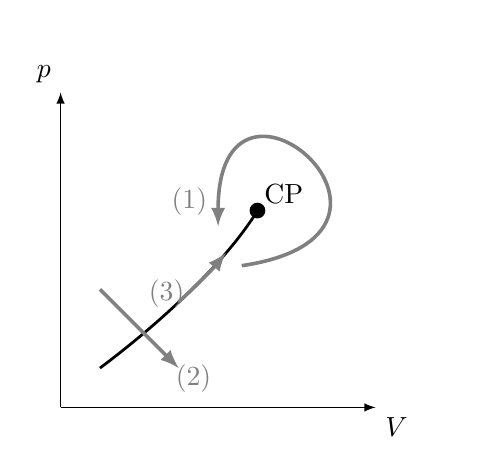
\begin{tikzpicture}
      \draw[-latex] (0,0) -- (4,0) node[below right] {$V$};
      \draw[-latex] (0,0) -- (0,4) node[above left] {$p$};
      \draw[line width=1pt] (0.5,0.5) .. controls (1.5,1.25) and (2.2,2.0) .. (2.5,2.5);
      \fill (2.5,2.5) circle (0.1) node[above right=-1pt] {CP};
      \draw[-latex,gray,line width=1.3pt] (0.5,1.5) -- (1.5,0.5) node[below right=-5pt] {$(2)$};
      \draw[-latex,gray,line width=1.3pt] (2.3,1.8) .. controls (5,2.2) and (2,4.8) .. (2,2.3) node[above left ] {$(1)$};
      \draw[-latex,gray,line width=1.3pt] (1.5,1.34) node[above left=-6pt]{$(3)$} .. controls (1.6,1.43) and (1.9,1.72) .. (2.1,1.965);
     \end{tikzpicture}
    }
    \caption{A szabadentalpia a nyomás függvényében (a), illetve speciális átalakulások a kritikus pont körül (b).}\label{fig:B09-gpspecatal}
   \end{figure}
    
   \paragraph{A kritikus pont körüli átalakulások} Speciális átalakulásokat mutat \aref{fig:B09-specatal}. ábra:

   \begin{enumerate}
    \item[(1)] Ekkor nem haladunk át fázishatáron, így a gőz/gáz/folyadék között nem látjuk sosem a különbséget.
   Ezen az úton nem történik fázisátalakulás, minden termodinamikai mennyiség analitikusan változik.
    \item[(2)] Áthaladunk a fázishatáron, elsőrendű fázisátalakulás történik.
   A fázishatáron különbséget látunk a folyadék és a gőz között, az egyik fázis moláris térfogata jóval nagyobb, mint a másiké. 
    \item[(3)] A fázishatáron haladva látjuk a különbséget a gőz és a folyadék között (a moláris térfogat különbözik).
   A kritikus pont felé haladva a sűrűségkülönbség csökken, és a kritikus pontban nullává válik.
   Ahogy áthaladunk a kritikus ponton, már csak egy fázist látunk.
   Mivel a $\Delta V$ folytonosan vált nullává, ez az átalakulás folytonos: másodrendű.
   \end{enumerate}

  \section{Univerzalitás}
   
   Lásd \aref{ss:B10-univerzalitas}. fejezetben.

  \chapter{Landau-elm\'elet, sk\'al\'az\'as} 

 \section{Rendparaméter}
   
  A rendparaméter ($\psi$) egy olyan mennyiség, aminek értékével közvetlenül jellemezni tudjuk azt, hogy melyik fázisban vagyunk. $\psi$ egy olyan mennyiség, ami a szimmetrikus fázisban nulla, a szimmetriasértőben pedig véges értéket vesz fel.
   Legyen $G_{sz}$ a szimmetrikus fázis csoportja, míg $G_{nsz}$ a szimmetriasértőé.
   Másodrendű az átalakulás, ha $G_{nsz}\subset G_{sz}$, ugyanis ekkor egy paraméter folytonos változtatásával elérhető, hogy a szimmetrikus fázis szimmetriacsoportja $G_{nsz}$-ra szűküljön.
   Ha $G_{nsz}\nsubseteq G_{sz}$, akkor az átalakulás biztos, hogy elsőrendű.
  
  A rendparaméterhez tartozik egy konjugált tér, mellyel el lehet érni, hogy a szimmetrikus fázisban is véges értéket vegyen fel.
   Ilyen pl.\ $H$ az FM--PM átalakulásnál, de nincs ilyen valós tér pl.\ az AFM--FM átalakulásnál. 
 
 \section{Landau-elmélet}
 
  A Landau-elmélet alapvető célja, hogy a szabadenergia(-sűrűség)-et felírja mint egy kis paraméter Taylor-soraként a kritikus pont közelében.
   Ez a kis paraméter a rendparaméter lesz.
   A ferromágneses--paramágneses átalakulás nyelvezetét használva ($\psi=m$) írjuk fel az elméletet.
   Az alapfeltevések a következőek:
  \begin{itemize}
   \item $\TC$ környékén a a mágnesezettségi sűrűsége nagyon pici: $m\xrightarrow{T\to\TC}0$,
   \item az állapotok eloszlása nagyon éles $m$ szerint, így az $m$ várható értéke és legvalószínűbb értéke megegyezik,
   \item illetve az eloszlások közelíthetőek Gauss-görbével. (Ez a fluktuációk meghatározásánál lesz hasznos.)
  \end{itemize}
  
  A (mágneses) szabadenergia-sűrűség sorfejtése negyedrendig:
  \al{
   f(T,H,m)=w(T)+\frac{a(T)}{2}m^2+\frac{u(T)}{4}m^4-Hm.
  }
  Mágneses tér nélkül az energia invariáns $m$ előjelétől, így $m$-nek csak páros hatványai szerepelhetnek.
   Minden hatvány együtthatója függhet $T$-től.
   Elvárjuk, hogy $u(T)$ pozitív legyen minden $T$-re, hogy létezzen globális minimum. 
  
  Egyensúly ott van, ahol $m$ minimalizálja $f$ értékét:
  \al{
   &0=\pder{f}{m}=a(T)m+u(T)m^3-H
   &0<\pder{^2 f}{m^2}=a(T)+3 u(T)m^2
  }
  
  $H=0$ esetben az $m=0$ jó megoldás.
   Az egyensúlyi feltétel akkor teljesül, ha $a(T)>0$.
  
  $m\ne 0$ megoldás esetében $m=\sqrt{-\frac{a(T)}{u(T)}}$.
   Az egyensúlyi feltétel: $0<a(T)+3 u(T)m^2=a(T)-3u(T)\frac{a(T)}{u(T)}=-2a(T)$, tehát itt $a(T)$ negatív. 
  
  Legyen $\TC$ az a hőmérséklet, ahol $a(T)$ előjelet vált.
   Legegyszerűbb közelítésben $a(T)=a_0(T-\TC)$ és $u(T)=u_0$.
   Az állapotegyenlet megoldását \aref{fig:B10-landau}. ábra mutatja.
  
  \begin{figure}[ht!]
   \centering
   \subfloat[Az állapotegyenlet megoldása $m(T,H)$-ra.\label{fig:B09-l1}]{\includegraphics[width= 0.5\textwidth]{./B09tetel/thm}} \\
   \subfloat[Fix mágneses tér mellet az $m(T)$ függvény.\label{fig:B09-l2}]{\includegraphics[width= 0.3\textwidth]{./B09tetel/TM}} \hspace{6pt}
   \subfloat[Fix hőmérséklet mellet az $m(H)$ függvény.\label{fig:B09-l3}]{\includegraphics[width= 0.3\textwidth]{./B09tetel/HM}} \hspace{6pt}
   \subfloat[Fix mágnesezettség mellet az $H(T)$ függvény.\label{fig:B09-l4}]{\includegraphics[width= 0.3\textwidth]{./B09tetel/HT}} 
   \caption{A negyedrendű szabadenergia sorfejtéssel felírt Landau-elmélet  állapotegyenlete és annak szintvonalai mindhárom síkra vetítve.
   Az (a) ábrán látszik, hogy hol hányadrendű az átalakulás: a $H=0$, $T<T_\text{C}$ vonalon $m=\pder{f}{H}$ ugrik, vagyis is elsőrendű az átalakulás, míg $H=0$, $T=T_\text{C}$-ben $m$ érintője, vagyis $\pder{^2 f}{H^2}$ vagy $\pder{^2 f}{H\partial T}$ vagy $\pder{^2 f}{T^2}$ divergál, vagyis az átalakulás abban a pontban másodrendű.}\label{fig:B10-landau}
  \end{figure}
  
  Vezessük be $\tau=T-\TC$-t, a relatív hőmérsékletet.
  Eddig tehát tudjuk, hogy
  \al{
   m=\begin{cases}
      0 & T<\TC\\
      \sqrt{\frac{a_0}{u_0}}\abs{\tau}^{\frac{1}{2}} & T>\TC,
     \end{cases}
  } 
  vagyis $\beta=\frac{1}{2}$.
  
  $T=\TC$-n a mágnesezettség tértől való függését is fel tudjuk írni.
   Az egyensúlyra vonatkozó egyenletek alapján:
  \al{
   &H=u_0m^3
   &m=\abs{\frac{H}{u}}^{\frac{1}{3}}\sim \abs{H}^\frac{1}{3},
  }
  ahonnan $\delta=\frac{1}{3}$.
  
  Az $m(T)$-ből a szuszceptibilitás, felhasználva az egyensúlyra vonatkozó egyenleteket:
  \al{
   \chi^{-1}=\pder{H}{m}=\pder{^2 f}{m^2}=a(T)+3 u(T)m^2
    =\begin{cases}
      T<\TC: &-2a(T)=2a_0\abs{\tau}\\
      T>\TC: &\phantom{-2}a(T)=a_0\abs{\tau}
     \end{cases}
  }
  vagyis s szuszceptibilitás divergál $T=\TC$-n, csak két oldalról kicsit más együtthatóval.
   Az exponens $\gamma=1$. 
  
  A szabadenergia az egyensúlyban és $H=0$ esetben:
  \al{
   F(T,H=0)
    &=\min_{M}F(T,H,M)
     =V\min_{m}\left(w(T)+\frac{a(T)}{2}m^2+\frac{u(T)}{4}m^4\right)\\
    &=\begin{cases}
       T<\TC:& V\left(w(T)-\frac{a_0^2\tau^2}{4u_0}\right) \\
       T>\TC:& Vw(T)
      \end{cases}
  }
  A hőkapacitás:
  \al{
   C_V=-T\pder{^2F }{T^2}
    =\begin{cases}
      T<\TC:& -TV\pder{^2 w(T)}{T^2}+TV\frac{a_0^2}{2u_0} \\
      T>\TC:& -TV\pder{^2 w(T)}{T^2}
     \end{cases}
  }
  vagyis $T=\TC$-n a fajhőnek ugrása van: $C(\TC-0)-C(\TC+0)=TV\frac{a_0^2}{2u_0}$, így a fajhő kritikus exponens $\alpha=0$.
  
  A fluktuációk számításához a paramágneses fázisban felhasználjuk, hogy $P(M)\sim e^{-\beta F(T,H,M)}$. $H=0$ esetben, csak a másodrendű tagot megtartva:
  \al{
   &P(M)\sim e^{-\beta V\frac{a(t)}{2}m^2}
   &\Rightarrow
   &&\mv{(\Delta m)^2}&=\frac{1}{\beta V a(T)}=\frac{\kB T}{V a(T)}=\frac{\kB T}{V}\chi\\
   &&&&\mv{(\Delta M)^2}&=\kB T V\chi.
  }
  
  A korrelációs függvény kiszámításához inhomogén mágneses teret és inhomogén mágnesezettséget kell bevezetni.
   Az $f$-ben $m=m_\text{eq}+\delta m(\rv)$, ahol $\delta m(\rv)$ a helyfüggő kis moduláció a mágnesezettségben.
   Ekkor a szabadenergia sorfejtésébe bele kell venni az $m(\rv)$ gradiensét is egy $\frac{c}{2}\abs{\grad{m(\rv)}}^2$ taggal. $f$ kifejtve, majd Fourier-transzformálva Gauss-alakú lesz, ahonnan a fluktuáció nagysága leolvasható.
   Innen a szuszceptibilitás kifejezhető:
  \al{
   &\chi(q)=\frac{1}{c}\frac{1}{q^2+\xi^{-2}}
   &\xi=\sqrt{\frac{c}{a(T)+3u_0m^2}}.
  }
  A korrelációs függvény:
  \al{
   &C(q)=\beta^{-1}\chi(q)
    =\frac{\kB T}{c}\frac{1}{q^2+\xi^{-2}}
   &C(r)=\frac{\kB T}{c}\frac{1}{4\pi}\frac{e^{-r/\xi}}{r},
  }
  így tehát $\xi$ a korrelációs hossz, mely
  \al{
   \xi^{-2}=\frac{1}{c}\big(a(T)+3u_0m^2\big)
    =\begin{cases}
      H=0, T<\TC, \left(m^2=-\frac{a(T)}{u_0}\right): & 2\frac{a_0\abs{\tau}}{c}\\
      H=0, T>\TC, \left(m=0\right): & \frac{a_0\abs{\tau}}{c}\\
      H\ne 0, T=\TC, \left(a=0,H=u_0m^3\right): & \frac{3u_0}{c}\left(\frac{H}{u_0}\right)^{\frac{3}{2}}
     \end{cases}
  }
  Inenn mindjárt látszik, hogy $H=0$-ra $\xi\sim \abs{\tau}^{-\nu}$, $\nu=\frac{1}{2}$. és $T=\TC$-re $\xi\sim \abs{H}^{-\mu}$, $\mu=\frac{1}{3}$. $C(q)$ $\tau=0$ és $H=0$-ra $C(r)\sim r^{-d+2-\eta}$, ahol $d=3$ a dimenziószám, így $\eta=0$.
  
 \section{Ginzburg-kritérium}
  
  A Landau-elmélet dimenziófüggetlen, de a fázisátalakulások nem azok.
   Nézzük meg, hogy a Landau-elmélet konzisztens-e. 
  
  Számoljuk ki a mágnesezettség fluktuációit:
  \al{
   \mv{\Delta M^2}
   &=\intl{V}{}\drh\intl{V}{}\drkh\mv{m(\rv)-m_\text{eq}}\mv{m(\rv')-m_\text{eq}}
    =\intl{V}{}\drh\intl{V}{}\drkh C(\rv-\rv')\\
   &=V\intl{V}{}\drh C(\rv)
    =VC(q=0)
    =V\kB T \chi(q=0)
    =V\kB T \chi
  }
  A relatív fluktuáció:
  \al{
   \frac{\mv{\Delta M^2}}{M^2}
    =\frac{V\kB T \chi}{M^2}
    =\frac{\kB T \chi}{V m^2}.
  }
  A korrelációk csak $\xi^d$ tartományban vannak, így a minta térfogata helyett ebben a térfogatban tekintsük a relatív fluktuációkat.
   Ekkor a hőmérséklettől való függés:
  \al{
   \frac{\mv{\Delta M^2}}{M^2}
    =\frac{\kB T \chi}{\xi^d m^2}
    \sim\frac{\abs{\tau}^{-1}}{\abs{\tau}^{-d/2}\cdot\abs{\tau}^{2\cdot 1/2}}
    \sim \abs{\tau}^{d/2-2}.
  }
  Az elmélet akkor használható, ha $\tau\to 0$-re a szabadenergia-sűrűség sorfejtése értelmes, azaz, ha a fluktuációk nem robbannak fel.
   Ehhez szükséges, hogy $d/2-2\ge 0$, vagyis $d\ge 4$.
   Tehát a Landau-elmélet szigorúan véve csak négy, vagy annál nagyobb dimenzióban értelmes.
  
  Praktikusan ez alacsony dimenzióban a Landau-elméletnek egy korlátot ad, hogy meddig érvényes.
   Annyira közelíthetjük meg $\TC$-t, hogy ez a fluktuációs tag még $\sim\mathcal{O}(1)$ legyen.
  
 \section{Skálahipotézis, skálázás}
  
  A sálahipotézis abból, áll, hogy feltesszük, hogy a rendszerben egyetlen karakterisztikus hosszúság van, a korrelációs hossz. 
  
  A korrelációs függvény ekkor: $C(q,\xi)=C(q=0,\xi)\cdot\phi(q\xi)$, ugyanis másképp nem függhet $q$-tól.
   Tudjuk, hogy $C(q=0)\sim\chi\sim\abs{\tau}^{-\gamma}$, illetve $\xi\sim\abs{\tau}^{-{\nu}}$, így $C(q=0)\sim\xi^{\frac{\gamma}{\nu}}$, vagyis
  \al{
   C(q,\xi)=\xi^{\frac{\gamma}{\nu}}\cdot\phi'(q\xi).
  }
  Ez egy általánosított homogén függvény, hiszen
  \al{
   &C\left(\lambda q,\frac{\xi}{\lambda}\right)
    &=\left(\frac{\xi}{\lambda}\right)^{\frac{\gamma}{\nu}}\phi'\left(\lambda q\frac{\xi}{\lambda}\right)
     =\lambda^{-\frac{\gamma}{\nu}}C\left(q,\xi\right)
   &\Rightarrow
   &&C\left(q,\xi\right)=\lambda^{\frac{\gamma}{\nu}}C\big(\lambda q,\lambda^{-1}\xi\big).
  }
  Visszaírva a $\tau$ függést: $\xi=\xi_0\abs{\tau}^{-\nu}$ $\rightarrow$ $\lambda^{-1}\xi=\xi_0\left(\lambda^{\frac{1}{\nu}}\abs{\tau}\right)^{-\nu}$, vagyis $C(q,\tau)=\lambda^{\frac{\gamma}{\nu}}C\big(\lambda q,\lambda^{\frac{1}{\nu}}\tau\big)$. 
  
  Teljesen hasonlóan le lehet vezetni a $H$-tól való függést $\xi$-n keresztül. Összegezve:
  \al{
   C\left(q,\tau,H\right)=\lambda^{\frac{\gamma}{\nu}}C\Big(\lambda q,\lambda^{\frac{1}{\nu}}\tau,\lambda^{\frac{1}{\mu}}H\Big),
  }
  ami még mindig egy hipotézis, csak jól argumentált. 
  A korrelációs függvényre hasonló skálahipotézis adható.
   Ez úgy adható meg, hogy $\xi$ az a távolság ami alatt a korrelációs függvény a felére csökken: $C(q=\frac{1}{\xi})=\frac{1}{2}C(q=0)$, ennek kifejtéséből:
  \al{
   \xi(\tau,H)=\lambda \xi\Big(\lambda^{\frac{1}{\nu}}\tau,\lambda^{\frac{1}{\mu}}H\Big).
  }
  A korrelációs függvényre vonatkozó skálahipotézisből a szuszceptibilitás ($\chi=\beta C(q=0)$): $\chi(\tau,H)=\lambda^{\frac{\gamma}{\nu}}C\big(\lambda^{\frac{1}{\nu}}\tau,\lambda^{\frac{1}{\mu}}H\big)$, ahol $\lambda'=\lambda^{\frac{1}{\nu}}$-t bevezetve
  \al{
   \chi(\tau,H)=\lambda^{\gamma}\chi\Big(\lambda\tau,\lambda^{\frac{\nu}{\mu}}H\Big). 
  }
  A mágnesezettség: $\chi=\pder{m}{H}$, vagyis akkor 
  \al{
   m(\tau,H)=\lambda^{\gamma-\frac{\nu}{\mu}}m\Big(\lambda\tau,\lambda^{\frac{\nu}{\mu}}H\Big)
  }
  kell, hogy legyen.
   Hasonlóan a szabadenergia-sűrűség:
  \al{
   f(\tau,H)=\lambda^{\gamma-2\frac{\nu}{\mu}}f\Big(\lambda\tau,\lambda^{\frac{\nu}{\mu}}H\Big).
  }
  
  \subsection{Összefüggések a kritikus exponensek között}
   \begin{itemize}
    \item A korrelációs hossz, ha $H=0$, és $\lambda=\abs{\frac{\tau}{\tau_0}}^{-\nu}$:
    \al{
     \xi(\tau,0)
      =\lambda \xi\Big(\lambda^{\frac{1}{\nu}}\tau,0\Big)
      =\abs{\frac{\tau}{\tau_0}}^{-\nu} \xi\left(\abs{\frac{\tau}{\tau_0}}^{\frac{-\nu}{\nu}}\tau,0\right)
      =\abs{\frac{\tau}{\tau_0}}^{-\nu} \underbrace{\xi\Big(\pm\tau_0,0\Big)}_{=\text{konst}}
      \sim \abs{\tau}^{-\nu},
    }
    illetve ha $\tau=0$ és $\lambda=\abs{\frac{H}{H_0}}^{-\mu}$:
    \al{
    \xi(0,H)
     =\lambda \xi\Big(0,\lambda^{\frac{1}{\mu}}H\Big)
     =\abs{\frac{H}{H_0}}^{-\mu} \xi\left(0,\abs{\frac{H}{H_0}}^{\frac{-\mu}{\mu}}H\right)
     =\abs{\frac{H}{H_0}}^{-\mu} \underbrace{\xi\left(0,\pm H_0\right)}_{=\text{konst}}
     \sim \abs{H}^{-\mu}.
    }
    
    \item A szuszceptibilitás $H=0$-ra és $\lambda=\abs{\frac{\tau_0}{\tau}}$-t választva:
    \al{
     \chi(\tau,0)
      =\lambda^{\gamma}\chi\Big(\lambda\tau,0\Big)
      =\abs{\frac{\tau_0}{\tau}}^{\gamma}\chi\Big(\abs{\frac{\tau_0}{\tau}}\tau,\lambda^{\frac{\nu}{\mu}}H\Big)
      =\abs{\frac{\tau_0}{\tau}}^{\gamma}\underbrace{\chi\Big(\pm\tau_0,0\Big)}_{=\text{konst}}
      \sim\abs{\tau}^{-\gamma}
    }
    
    \item A korrelációs függvény $\tau=0$ és $H=0$-ra, $\lambda=\frac{q_0}{q}$ választással
    \al{
     C\left(q,0,0\right)
      =\lambda^{\frac{\gamma}{\nu}}C\Big(\lambda q,0,0\Big)
      =\left(\frac{q_0}{q}\right)^{\frac{\gamma}{\nu}}C\left(\frac{q_0}{q} q,0,0\right)
      =\left(\frac{q_0}{q}\right)^{\frac{\gamma}{\nu}}\underbrace{C\left(q_0,0,0\right)}_{=\text{konst}}
      \sim q^{-\frac{\gamma}{\nu}}.
    }
    Az $\eta$ kritikus exponenst úgy definiáltuk, hogy $C(q)\sim q^{-2+\eta}$, így $-2+\eta=-\frac{\gamma}{\nu}$ azonnal adódik.
    
    \item A mágnesezettségi sűrűségből $H=0$ esetben $\lambda=\abs{\frac{\tau_0}{\tau}}$-t választva:
    \al{
     m(\tau,0)
      =\lambda^{\gamma-\frac{\nu}{\mu}}m\Big(\lambda\tau,0\Big)
      =\abs{\frac{\tau_0}{\tau}}^{\gamma-\frac{\nu}{\mu}}m\Big(\abs{\frac{\tau_0}{\tau}}\tau,0\Big)
      =\abs{\frac{\tau_0}{\tau}}^{\gamma-\frac{\nu}{\mu}}\underbrace{m\Big(\pm\tau_0,0\Big)}_{=\text{konst}}
      \sim \abs{\tau}^{-\gamma+\frac{\nu}{\mu}}.
    }
    Szintén a korábbi $\beta$ exponens definíciójából $\beta=-\gamma+\frac{\nu}{\mu}$.
   Hasonlóan $\tau=0$, $
    \lambda=\abs{\frac{H_0}{H}}^{-\frac{\mu}{\nu}}$.
    \al{
     m(0,H)
      &=\lambda^{\gamma-\frac{\nu}{\mu}}m\Big(0,\lambda^{\frac{\nu}{\mu}}H\Big)
      =\abs{\frac{H_0}{H}}^{-\frac{\mu}{\nu}\gamma+1}m\Big(0,\abs{\frac{H_0}{H}}H\Big)
      =\abs{\frac{H_0}{H}}^{-\frac{\mu}{\nu}\gamma+1}\underbrace{m\Big(0,\pm H_0\Big)}_{=\text{konst}}\\
      &\sim\abs{H}^{\frac{\mu}{\nu}\gamma-1}.
    }
    Szintén a korábbi definícióval való összevetésből: $\frac{1}{\delta}=-\frac{\mu}{\nu}\gamma+1$.
    
    \item Végül a fajhőhöz $f$, ha $H=0$: válasszuk $\lambda=\abs{\frac{\tau_0}{\tau}}$,
    \al{
     f(\tau,0)
     &=\lambda^{\gamma-2\frac{\nu}{\mu}}f\Big(\lambda\tau,0\Big)
      =\abs{\frac{\tau_0}{\tau}}^{\gamma-2\frac{\nu}{\mu}}f\Big(\abs{\frac{\tau_0}{\tau}}\tau,0\Big)
      =\abs{\frac{\tau_0}{\tau}}^{\gamma-2\frac{\nu}{\mu}}\underbrace{f\Big(\pm\tau_0,0\Big)}_{=\text{konst}}
      \sim \abs{\tau}^{-\gamma+2\frac{\nu}{\mu}}.
    }
    Innen a fajhő $\tau$ függése megadható, hiszen az a szabadenergia-sűrűség második deriváltjával arányos.
   A két deriválás a kitevőben $-2$-t hoz be, így $C\sim\pder{^2 f}{T^2}\sim \abs{\tau}^{-\gamma+2\frac{\nu}{\mu}-2}$.
   A korábbi definíció alapján így: $\alpha=\gamma-2\frac{\nu}{\mu}+2$.
   Ennek az egyenlőségnek az átírásához felhasználjuk a $\beta$-ra vonatkozó egyenletet: $\alpha=-2\beta-\gamma+2$.
   \end{itemize}
   
   Összefoglalva:
   \al{
     C&\sim\abs{\tau}^{-\alpha} && H=0\\
     m&\sim\abs{\tau}^{\beta} && H=0\\
     \chi&\sim\abs{\tau}^{-\gamma} && H=0\\
     m&\sim\abs{H}^{\frac{1}{\delta}} && \tau=0\\
     \xi&\sim\abs{\tau}^{-\nu} && H=0\\
     \xi&\sim\abs{H}^{-\mu} && \tau=0\\
     C(q)&\sim \frac{1}{q^{2-\eta}} \;\Leftrightarrow \; C(r)\sim \frac{1}{r^{d-2+\eta}}&& \tau=0,H=0,
   }
   illetve a skálatörvények:
   \al{
    &\gamma=\nu(2-\eta)
    &\beta=-\gamma+\frac{\nu}{\mu}
    &&\frac{1}{\delta}=\frac{\nu-\mu\gamma}{\nu}
    &&2-\alpha=2\beta+\gamma.
   }
   Tehát $\gamma,\mu,\nu$-vel ki lehet fejezni az összes exponenst.
   Ez a három exponens határozza meg az univerzalitási osztályokat. 
   \paragraph{Hiperskálatörvény}
    
    Ezeken felül még egy skálatörvény belátható, ami a dimenziószámot is figyelembe veszi.
   A Ginzburg-kritériumnál láttuk, hogy 
    \al{
     \frac{\mv{\Delta M^2}}{M^2}
    =\frac{\kB T \chi}{V m^2}.
    }
    
    Azt láttuk, hogy egy korrelációs hossznyi tartományban ez csak akkor nem divergál $T\to\TC$-re, ha $d\ge 4$.
   Ha ez mégis divergálna, akkor létezne egy nagyobb térfogat, $R^d$, ahol a relatív fluktuáció $\sim\mathcal{O}(1)$.
   De ez ellentmondás, mert a skálahipotézis kimondja, hogy nem létezik más karakterisztikus távolság, csak $\xi$, úgyhogy annak kell igaznak lennie, hogy 
    \al{
    \mathcal{O}(1)\sim
     \frac{\kB T \chi}{\xi^d m^2}
     \sim\frac{\abs{\tau}^{-\gamma}}{\abs{\tau}^{-d\nu}\cdot\abs{\tau}^{2\cdot \beta}}
    \sim \abs{\tau}^{d/\nu-2\beta-\gamma},
    }
    vagyis $d/\nu-2\beta-\gamma=0$, ahonnan a hiperskálatörvény:
    \al{
     d\nu=2\beta+\gamma.
    }
    Az Ising-exponensekkel így az jön ki, hogy a Landau-elmélet csak $d=4$ dimenzióban korrekt.

 \section{Univerzalitás}\label{ss:B10-univerzalitas}
  
  A másodrendű fázisátalakulások rengeteg rendszerben jelen vannak.
   A megfigyelés az, hogy látszólag teljesen különböző rendszerek is ugyanazt a viselkedést mutatják a kritikus pont közelében. 
  
  Ennek magyarázata az, hogy ahogy a rendszer egyre közelebb kerül a kritikus ponthoz, úgy az egyre inkább skálafüggetlenné válik.
   Emiatt a rendszernek minden skáláfüggő tulajdonsága elvész, és csak a néhány releváns, skálafüggetlen tulajdonság marad. 
  
  A kritikus pont közelében a rendszerek hasonlósága abban nyilvánul meg, hogy a kritikus exponensek megegyeznek.
   Ez alapján a hasonló rendszereket univerzalitási osztályokba lehet sorolni.
   Az XY-osztályba tartozik például az az XY-Heisenbeg-model, a szupravezetés és a szuperfolyékonyság; az Ising-osztályba tartozik az Ising-modell, a folyadék--gáz fázisátalakulások és az uniaxiális mágnesek.
   A Heisenberg-osztályba az izotrop mágnesek és a Heisenberg-modell. 

  \chapter{Line\'aris v\'alasz, Kubo-formula, fluktu\'aci\'o--disszip\'aci\'o-t\'etel, kauzalit\'as} 
 
 \section{Lineáris válasz}
  
  Az időfüggetlen lineáris választ lásd \aref{ss:B05-linvalasz}. fejezetben.
   Itt az időfüggő válasszal fogunk foglalkozni kvantumos esetben.
  
  A rendszer Hamilton-operátora:
  \al{
   \opH=\opH_0-\opY F(t)
       =\opH_0+\opV(t),
  }
  ahol $F$ külső időfüggő perturbációkét jelen lévő klasszikus tér, mely az $\opY$ operátoron keresztül csatolódik.
   A perturbálatlan rendszer megoldását ismerjük, a kérdés az, hogy az időfüggő perturbációra hogyan változik meg a mérhető mennyiségek (pl. $\opX$) várható értéke. 
  
  Kis perturbációt tekintünk, úgyhogy $\mv{\opX}$ változását a perturbáció lineáris függvényeként keressük:
  \al{
   \mv{\Delta \opX(t)}
    =\mv{\opX(t)}_{F}-\mv{\opX(t)}_0
    =\intl{-\infty}{t}\dd t'\,\chi_{\opX\opY}(t-t')F(t').
  }
  Az egyenlet már magában hordozza a kauzalitást, ugyanis $\opX$ várható értékét csak a múltbeli események befolyásolhatják. 
  
  A perturbálatlan rendszerben a várható érték:
  \al{
   \mv{\opX}_0=\tr\left(\op\rho_0 \opX\right)=\frac{1}{\tr(\op\rho_0)}\suml{n}{}\bra{n}\opX\ket{n}e^{-\beta E_n}.
  }
  
  A perturbáció kezeléséhez tekintsük a rendszer Dirac-képben (lásd \aref{ss:A01-dirac}. fejezetet).
   Itt az operátorok a $\opH_0$ szerint fejlődnek, míg a hullámfüggvények a perturbáció szerint:
  \al{
   &\hat{X}(t)=e^{\frac{i}{\hbar}\opH_0 t}\op{X} e^{-\frac{i}{\hbar}\opH_0 t}
   &\ket{n(t)}=\T e^{-\frac{i}{\hbar}\intl{-\infty}{t}\dd \tau \op{V}_i(\tau)}\ket{n}.
  }
  Mivel a perturbáció kicsi, ezért a hullámfüggvények időfejlődését leíró operátort sorfejtjük, és csak az elsőrendű tagot tartjuk meg:
  \al{
   \T e^{-\frac{i}{\hbar}\intl{-\infty}{t}\dd \tau \op{V}_i(\tau)}
    &\approx 1-\frac{i}{\hbar}\intl{-\infty}{t}\dd \tau \op{V}_i(\tau).
  }

  Ezzel a kölcsönhatási képben az új sűrűségoperátor és az új várható érték:
  \al{
   &\op\rho(t)=\suml{n}{}\ket{n(t)}\bra{n(t)}e^{-\beta E_n}
   &\tr{\op\rho}=\suml{n}{}e^{-\beta E_n}=\tr{\op\rho_0}.
  }
  \al{
   \mv{\opX}_F
   &=\tr\left(\op\rho(t) \opX(t)\right)
    =\frac{1}{\tr(\op\rho_0)}\suml{n}{}\bra{n(t)}\opX(t)\ket{n(t)}e^{-\beta E_n}\\
   &=\frac{1}{\tr(\op\rho_0)}\suml{n}{}\bra{n}\left(1+\frac{i}{\hbar}\intl{-\infty}{t}\dd \tau \op{V}_i(\tau)\right)\opX(t)\left(1-\frac{i}{\hbar}\intl{-\infty}{t}\dd \tau \op{V}_i(\tau)\right)\ket{n}e^{-\beta E_n}\\
   &\approx\frac{1}{\tr(\op\rho_0)}\suml{n}{}\bra{n}\opX(t)\ket{n}e^{-\beta E_n}\\
   &\qquad+\frac{1}{\tr(\op\rho_0)}\suml{n}{}\bra{n}
     \left(
      \frac{i}{\hbar}\intl{-\infty}{t}\dd \tau \op{V}_i(\tau)\opX(t)
      -\opX(t)\frac{i}{\hbar}\intl{-\infty}{t}\dd \tau \op{V}_i(\tau)
     \right)
    \ket{n}e^{-\beta E_n}\\
   &=\frac{1}{\tr(\op\rho_0)}\suml{n}{}\bra{n}\opX(t)\ket{n}e^{-\beta E_n}
    +\frac{i}{\hbar}\intl{-\infty}{t}\dd \tau\,\frac{1}{\tr(\op\rho_0)}\suml{n}{}\bra{n}\left[\op{V}(\tau),\opX(t)\right]\ket{n}e^{-\beta E_n}\\
   &=\mv{\opX(t)}_0+\frac{i}{\hbar}\intl{-\infty}{t}\dd \tau\,\mv{\left[\op{V}(\tau),\opX(t)\right]}_0,
  }
  ahonnan leolvashatjuk a válaszfüggvényt:
  \al{
   \boxed{\chi_{\opX\opY}(t)=\frac{i}{\hbar}\mv{\left[\opX(t),\opY(0)\right]}_0\Theta(t).}
  }
  A Kubo-formula tehát megadja, hogy milyen változás lesz az $\opX$ operátor várható értékében, ha az $\opY$ operátorral csatolunk egy külső teret a rendszerhez.
   A válasz csak a perturbálatlan rendszertől függ.
   Az időfejlődések az összefüggésben a kölcsönhatási képben értendőek.
   A képletben $\Theta(t)$ fejezi ki a kauzalitást. 
  
 \section{Kramers--Kronig-reláció}
  
  Fejtsük ki a Kubo-formulát mátrixelemekkel:
  \al{
   \chi_{\opX\opY}(t)
    &=\frac{i}{\hbar}\Theta(t)\frac{1}{Z_0}\suml{n}{}e^{-\beta E_n}\bra{n}\left[\opX(t),\opY(0)\right]\ket{n}\\
    &=\frac{i}{\hbar}\Theta(t)\frac{1}{Z_0}\suml{n}{}e^{-\beta E_n}\bra{n}\left(\opX(t)\opY(0)-\opY(0)\opX(t)\right)\ket{n}\\
    &=\frac{i}{\hbar}\Theta(t)\frac{1}{Z_0}\suml{n}{}e^{-\beta E_n}\bra{n}\left(e^{\frac{i}{\hbar}\opH_0 t}\op{X} e^{-\frac{i}{\hbar}\opH_0 t}\opY-\opY e^{\frac{i}{\hbar}\opH_0 t}\op{X} e^{-\frac{i}{\hbar}\opH_0 t}\right)\ket{n}\\
    &=\frac{i}{\hbar}\Theta(t)\frac{1}{Z_0}\suml{n,m}{}e^{-\beta E_n}\bra{n}\left(e^{\frac{i}{\hbar}\opH_0 t}\op{X} e^{-\frac{i}{\hbar}\opH_0 t}\big(\ket{m}\bra{m}\big)\opY-\opY \big(\ket{m}\bra{m}\big)e^{\frac{i}{\hbar}\opH_0 t}\op{X} e^{-\frac{i}{\hbar}\opH_0 t}\right)\ket{n}\\
    &=\frac{i}{\hbar}\Theta(t)\frac{1}{Z_0}\suml{n,m}{}e^{-\beta E_n}\bra{n}\left(e^{\frac{i}{\hbar}(E_n-E_m) t}\op{X}\big(\ket{m}\bra{m}\big)\opY-\opY \big(\ket{m}\bra{m}\big)\op{X} e^{\frac{i}{\hbar}(E_m-E_n) t}\right)\ket{n}\\
    &=\frac{i}{\hbar}\Theta(t)\frac{1}{Z_0}\suml{n,m}{}e^{-\beta E_n}\bigg(e^{\frac{i}{\hbar}(E_n-E_m) t}\underbrace{\bra{n}\op{X}\ket{m}}_{X_{nm}}\underbrace{\bra{m}\op{Y}\ket{n}}_{Y_{mn}}-\underbrace{\bra{n}\op{Y}\ket{m}}_{Y_{nm}}\underbrace{\bra{m}\op{X}\ket{n}}_{X_{mn}} e^{\frac{i}{\hbar}(E_m-E_n) t}\bigg)\\
    &=\frac{i}{\hbar}\Theta(t)\frac{1}{Z_0}\suml{n,m}{}\bigg(e^{-\beta E_n}e^{\frac{i}{\hbar}(E_n-E_m) t}X_{nm}Y_{mn}-e^{-\beta E_m}Y_{mn}X_{nm} e^{\frac{i}{\hbar}(E_n-E_m) t}\bigg)\\
    &=\frac{i}{\hbar}\Theta(t)\frac{1}{Z_0}\suml{n,m}{}\bigg(e^{-\beta E_n}-e^{-\beta E_m}\bigg)X_{nm}Y_{mn} e^{\frac{i}{\hbar}(E_n-E_m) t}
  }
  Kapcsoljuk be adiabatikusan a gerjesztő szinuszos jelet: $F=F(t)=F\cdot e^{-i\omega t} e^{\delta t}$, ahol $\delta \to 0+0$.
   Ekkor a válasz:
  \al{
   \mv{\Delta \opX(\omega)}=\chi_{\opX\opY}(\omega)\cdot F(t).
  }
  Bevezetve az $\omega_{nm}=\frac{1}{\hbar}(E_n-E_m)$ jelölést,
  \al{
   \chi_{\opX\opY}(\omega)
    &=\intl{-\infty}{\infty}\dd t\,\chi_{\opX\opY}(t)e^{i\omega t}e^{-\delta t}\\
    &=\frac{i}{\hbar}\frac{1}{Z_0}\intl{0}{\infty}\dd t\,e^{i\omega t}e^{-\delta t}\suml{n,m}{}\bigg(e^{-\beta E_n}-e^{-\beta E_m}\bigg)X_{nm}Y_{mn} e^{\frac{i}{\hbar}(E_n-E_m) t}\\
    &=\frac{i}{\hbar}\frac{1}{Z_0}\suml{n,m}{}\bigg(e^{-\beta E_n}-e^{-\beta E_m}\bigg)X_{nm}Y_{mn} \intl{0}{\infty}\dd t\,e^{i(\omega+\omega_{nm})t-\delta t}\\
    &=\frac{i}{\hbar}\frac{1}{Z_0}\suml{n,m}{}\bigg(e^{-\beta E_n}-e^{-\beta E_m}\bigg)X_{nm}Y_{mn} \frac{1}{-i(\omega+\omega_{nm})+\delta }\\
    &=-\frac{1}{\hbar}\frac{1}{Z_0}\suml{n,m}{}\bigg(e^{-\beta E_n}-e^{-\beta E_m}\bigg)X_{nm}Y_{mn}\frac{1}{(\omega+\omega_{nm})+i\delta }.
  }
  Itt felhasználjuk, hogy $\frac{1}{\omega+\omega_{nm}+i\delta}\xrightarrow{\delta\to 0}\mathcal{P}\left(\frac{1}{\omega+\omega_{nm}}\right)-i\pi\delta (\omega+\omega_{nm})$, így
  \al{
   \chi_{\opX\opY}(\omega)
    &=\chi_{\opX\opY}'(\omega)+i\chi_{\opX\opY}''(\omega)\\
   \chi_{\opX\opY}'(\omega)
    &=-\frac{1}{\hbar}\frac{1}{Z_0}\suml{n,m}{}\bigg(e^{-\beta E_n}-e^{-\beta E_m}\bigg)X_{nm}Y_{mn}\mathcal{P}\left(\frac{1}{\omega+\frac{1}{\hbar}(E_n-E_m)}\right)\\
   \chi_{\opX\opY}''(\omega)
    &=\frac{\pi}{\hbar}\frac{1}{Z_0}\suml{n,m}{}\bigg(e^{-\beta E_n}-e^{-\beta E_m}\bigg)X_{nm}Y_{mn}\delta \left(\omega+\frac{1}{\hbar}(E_n-E_m)\right).
  }
  A felbontás nem feltétlenül valós és képzetes részből áll, ugyanis a mátrixelemek lehetnek még komplex számok. 
  
  Az $\chi_{\opX\opY}'(\omega)$-ben a főérték integrálban nem szerepelnek az átmenethez tartozó frekvenciák, így ez a rendszer rugalmas válasza.
   Ezzel szemben a $\chi_{\opX\opY}''(\omega)$ tagban csak a rendszer energiaszintjei közötti átmenetek találhatóak, ez a disszipatív válasz.
   A két mennyiség nem független, fennáll közöttük a Kramers--Kronig-reláció:
  \al{
   \chi_{\opX\opY}'(\omega)=\frac{1}{\pi}\mathcal{P}\intl{-\infty}{\infty}\dd\omega'\,\frac{\chi_{\opX\opY}''(\omega')}{\omega'-\omega}.
  }
  
 \section{Fluktuáció--disszipáció-tétel}\label{ss:B11-fdt}
  
  Az időfüggő szimmetrizált korrelációs függvény:
  \al{
   C_{\opX\opY}(t)=\frac{1}{2}\mv{\opX(t)\opY(0)+\opY(0)\opX(t)}_0.
  }
  Egy $x$ fizikai mennyiség véges idejű Fourier-transzformáltja:
  \al{
   &x(\omega,T)=\frac{1}{2T}\intl{-T}{T}\dd t\,e^{i\omega t}x(t)
   &x^*(\omega,T)=x(-\omega,T),
  }
  ahonnan a spektrális sűrűség:
  \al{
   S_{xx}=\lim_{T\to\infty}x^*(\omega,T)x(\omega,T).
  }
  Stacioner folyamatokra a Wiener--Khintchin-tétel szerint a spektrális sűrűség megegyezik a korrelációs függvény Fourier-transzformáltjával:
  \al{
   S_{\opX\opY}(\omega)
    ={\color{red}\lim_{T\to\infty}\frac{1}{2T}}\intl{-T}{T}\dd t\,e^{i\omega t}C_{\opX\opY}(t)
    =C_{\opX\opY}(\omega)
    =\intl{-\infty}{\infty}\dd t\,e^{i\omega t}\frac{1}{2}\mv{\opX(t)\opY(0)+\opY(0)\opX(t)}_0
  }
  
  Az $S_{\opX\opY}$ a $\chi$-hez hasonlóan kifejthető (itt nincs $\delta$, hanem az idő szerinti integrál kiszámításakor jön be a Dirac-delta):
  \al{
   S_{\opX\opY}(\omega)
    &=\frac{1}{2}\frac{1}{Z_0}\suml{n,m}{}\bigg(e^{-\beta E_n}+e^{-\beta E_m}\bigg)X_{nm}Y_{mn}2\pi\delta\left(\omega+\frac{1}{\hbar}(E_n-E_m)\right)
  }
  A Dirac-delta miatt $E_m$ lecserélhető itt is és $\chi_{\opX\opY}''(\omega)$-ban is:
  \al{
  S_{\opX\opY}(\omega)
    &=\pi(1+e^{-\beta\hbar\omega})\frac{1}{Z_0}\suml{n,m}{}e^{-\beta E_n} X_{nm}Y_{mn}\delta\left(\omega+\frac{1}{\hbar}(E_n-E_m)\right)\\
  \chi_{\opX\opY}''(\omega)
    &=\frac{\pi}{\hbar}(1-e^{-\beta\hbar\omega})\frac{1}{Z_0}\suml{n,m}{}e^{-\beta E_n}X_{nm}Y_{mn}\delta \left(\omega+\frac{1}{\hbar}(E_n-E_m)\right),
  }
  ahonnan következik, hogy 
  \al{
   \boxed{S_{\opX\opY}(\omega)
    =\hbar\ctgh\left(\frac{1}{2}\beta\hbar\omega\right)\chi_{\opX\opY}''(\omega).}
  }
  
  Klasszikus határesetben $\hbar\to 0$, vagy $\hbar\omega\to 0$.
   Ekkor:
  \al{
   S_{\opX\opY}(\omega)
    =\frac{2}{\beta\omega}\underbrace{\frac{1}{2}\beta\hbar\omega\ctgh\left(\frac{1}{2}\beta\hbar\omega\right)}_{\to 1}\chi_{\opX\opY}''(\omega)
    =\frac{2\kB T}{\omega}\chi_{\opX\opY}''(\omega)
  }

  \chapter{Transzport, fluktu\'aci\'ok, id\H{o}f\"ugg\H{o} korrel\'aci\'ok, kereszteffektusok, Onsager-rel\'aciok} 
 
 \section{Időfüggő egyensúlyi korrelációs függvények}
  
  Legyen két időfüggő fizikai mennyiség $X(t)$ és $Y(t)$.
   Ezek átlaguktól való eltérése: $x(t)=X(t)-\mv{X}(t)$ és $y(t)=Y(t)-\mv{Y}(t)$.
   Az időfüggő korrelációs függvény:
  \al{
   C_{xy}(t)=\mv{x(t')y(t'+t)}_{t'}
    =\lim_{T\to\infty}\frac{1}{T}\intl{0}{T}\dd t'\, x(t')y(t+t').
  }
  Ha a rendszer stacioner és ergodikus, akkor az így definiált időátlag, $\mv{\,\cdot\,}_{t'}$, megegyezik a sokaságátlaggal, $\mv{\,\cdot\,}$.
   A korrelációs függvény tulajdonságai:
  \begin{itemize}
   \item 
    $t\to\infty$-re a korrelációk függetlenek lesznek egymástól:
    \al{
     \lim_{t\to\infty}C_{xy}(t)
      &=\lim_{t\to\infty}\mv{x(t')y(t'+t)}_{t'}
       =\lim_{t\to\infty}\mv{x(0)y(t)}
       =\mv{x(0)}\lim_{t\to\infty}\mv{y(t)}
       =0
    }
    
   \item
    $t=0$-ra az időfüggő korrelációs függvény megegyezik a keresztkorrelációs együtthatókkal:
    \al{
     C_{xy}(t=0)
      &=\mv{x(t')y(t')}_{t'}
       =\mv{x(0)y(0)}
    }
    
   \item 
    \al{
     C_{xy}(t)
      &=\mv{x(t')y(t'+t)}_{t'}
       =\mv{x(t'-t)y(t')}_{t'}
       =\mv{y(t')x(t'+(-t))}_{t'}
       =C_{yx}(-t)
    }
   \item 
    A korrelációs függvény szimmetrikus: $C_{xy}(t)=C_{yx}(t)$ (ha a rendszer időtükrözésre invariáns).
   Ehhez fejtsük ki a fenti sokaságátlagot:
    \al{
     C_{xy}(t)
      &=\intl{}{}\dd x\,\intl{}{}\dd y\, xy\cdot P(x) P(y,t|x) ,
    }
    ahol $P(x)$ annak a valószínűsége, hogy $x$ fluktuációja $x$, illetve $P(t,y|0,x) $ annak a valószínűsége, hogy $y$ a fluktuáció értéke $t$-ben, ha $t=0$-ban $x$ értéke $x$ volt.
   A részletes egyensúly következménye, hogy $P(x) P(t,y|0,x)=P(y) P(t,x|0,y)$.
   Ezt behelyettesítve:
    \al{
     C_{xy}(t)
      &=\intl{}{}\dd x\,\intl{}{}\dd y\, xy\cdot P(y) P(t,x|0,y)
       =C_{yx}(t).
    }
   
   \item 
    Az előző kettőből $C_{yx}(t)=C_{xy}(-t)$, vagyis a korrelációs függvény időben is szimmetrikus. 
  \end{itemize}
  
  A korrelációs függvények kiterjeszthetőek a kvantummechanikai esetre is.
   Itt azonban figyelembe kell venni, hogy az operátorok nem felcserélhetőek.
   Ehhez szimmetrizálni/antiszimmetrizálni kell:
  \al{
   C^{F/B}_{\opx\opy}=\frac{1}{2}\mv{\mv{\opx(t')\opy(t'+t)\pm\opy(t'+t)\opx(t')}}_{t'}.
  } 
  A belső várható érték a kvantummechanikai várható értéket jelenti, a külső pedig az időbelit.
   Az előbb bizonyított tulajdonságok továbbra is fennállnak. 
  
 \section{Lineáris transzport}
  
  Egyensúlyban a fluktuációk várható értéke nulla, azonban az értékük az egyes időpillanatokban nem nulla.
   Az fluktuáció oka a statisztikus jelleg, az, hogy az eloszlásnak van valamilyen szélessége.
   A fluktuáció véges értékét úgy is el tudjuk érni, hogy a rendszerre valamilyen külső teret kapcsolunk, majd ezt a teret kikapcsoljuk.
   Amíg a teret bekapcsoltuk, a rendszerbe beleavatkoztunk, így az nem-egyensúlyi állapotban van.
  
  Bárhogy is jött létre az átlagértéktől való eltérés, a várható értéke $t\to\infty$-re újra lecseng:
  \al{
   \lim_{t\to\infty}\mv{\xv(t)|\xv(t=0)=\xv_0}=0.
  }
  
  A nem egyensúlyi sokaságok lényege, hogy a valamilyen módon előállt $x_0$ makroállapotnak megfelelő sokaságot állítjuk elő, azzal a feltételes eloszlással, hogy $x_0$ fennáll.
   A rendszerben a dinamika változatlan, egyedül az eloszlás különbözik. 
  
  Térítsünk ki egy mennyiséget az egyensúlyi értékéből.
   Az átlaghoz való visszatérési sebessége ekkor arányos lesz a kitéréssel, vagyis:
  \al{
   \mv{\dot x_i}_{\xv_0}=-\suml{k}{}\lambda_{ik}\mv{x_k}_{\xv_0}.
  }
  Definiáljunk a termodinamikai erőt: $y_i=-\pder{S}{x_i}$.
   Az entrópia sorfejtése: $S=S_0-\frac{1}{2}\suml{ij}{}x_ig_{ij}x_j$, ahol $g_{ij}$ szimmetrikus.
   Innen $y_i=\suml{j}{}g_{ij}x_j$, ami megfordítva $x_i=\suml{j}{}\big[g^{-1}\big]_{ij}y_j$.
   Ezt felhasználva:
  \al{
   \mv{\dot x_i}_{\xv_0}
    =-\suml{k}{}\lambda_{ik}\suml{j}{}\big[g^{-1}\big]_{kj}\mv{y_j}_{\xv_0}
    =-\suml{j}{}\underbrace{\suml{k}{}\lambda_{ik}\big[g^{-1}\big]_{kj}}_{L_{ij}}\mv{y_j}_{\xv_0}
    =-\suml{j}{}L_{ij}\mv{y_j}_{\xv_0}
  }
  Ez a transzportegyenlet.
   A termodinamikai erőre másik definíciót is adhatunk.
   Az előző alapján felírhatjuk, hogy $\dd S=-\suml{i}{}y_i\dd x_i$.
   Innen az entrópiaprodukció: $\dot S=-\suml{i}{}y_i\dot x_i$, vagyis $y_i=-\pder{\dot S}{\dot x_i}$. 
  
  \subsection{Onsager-hipotézis}
   
   Az Onsager-hipotézis lényege, hogy az egyensúlyi fluktuációk és a nem egyensúlyi kitérítés között nincs különbség, miközben a rendszer relaxál mindegy, hogy mi volt az eredeti kitérés oka.
   Ez azt jelenti, hogy a transzportegyenlet a korrelációs függvényekre felírva is igaz:
   \al{
    \der{}{t}\mv{x_i(t),x_j(0)}=-\suml{k}{}L_{ik}\mv{y_k(t),x_j(0)}.
   }
   A hipotézis következményének belátásához felhasználjuk a korrelációs függvény szimmetrikusságát ($C_{ij}(t)=C_{ji}(t)$), illetve az alábbi azonosságot: $\mv{y_k x_j}=\kB\delta_{kj}$.
   Ennek belátásához nézzük a 
   \al{
    0
     &=N\intl{}{}\dd^{n}x\,\pder{}{x_j}\left(x_i e^{-\frac{1}{2\kB}\suml{lm}{}x_l g_{lm}x_m}\right)\\
     &=N\intl{}{}\dd^{n}x\,\underbrace{\pder{x_i}{x_j}}_{\delta_{ij}} e^{-\frac{1}{2\kB}\suml{lm}{}x_l g_{lm}x_m}+N\intl{}{}\dd^{n}x\,x_i\pder{}{x_j} e^{-\frac{1}{2\kB}\suml{lm}{}x_l g_{lm}x_m}\\
     &=\delta_{ij}+N\intl{}{}\dd^{n}x\,x_i \left(-\frac{1}{\kB}\suml{l}{} g_{jl}x_l\right)e^{-\frac{1}{2\kB}\suml{lm}{}x_l g_{lm}x_m}
      =\delta_{ij}-\frac{1}{\kB}\mv{x_i y_j}.
   }
   Az első egyenlőség triviálisan igaz, hiszen ha $x_j$ szerint kiintegrálunk, akkor az kiintegrált rész eltűnik a határokon. 
   
   Tehát használjuk fel a korrelációs függvény szimmetrikusságát:
   \al{
    &\der{}{t}\mv{x_i(t),x_j(0)}=\der{}{t}\mv{x_j(t),x_i(0)}
    &\Rightarrow&
    &-\suml{k}{}L_{ik}\mv{y_k(t),x_j(0)}=-\suml{k}{}L_{jk}\mv{y_k(t),x_i(0)},
   }
   majd tekintsük a relációt $t=0$-ban.
   Ekkor felhasználva a másik azonosságot:
   \al{
    L_{ij}=L_{ji}
   }
   adódik, ami az Onsager-féle reciprocitási törvény.
   Mivel a korrelációs törvény szimmetrikusságának követelménye az volt, hogy a mikroszkopikus folyamatok reverzibilisek, ezért ezt itt is meg kell követelni.
   Az időtükrözési invariancia lehetséges, hogy nem teljesül pl. mágneses tér jelenlétében, vannak olyan mennyiségek, amelyek előjelet váltanak az időtükrözésre.
   Ekkor $C_{xy}(t)=I_x I_y C_{yx}(t)$, ahol $I$ az időtökrözéshez tartozó sajátérték, és így $L_{xy}=I_x I_y L_{yx}$.
   
  \subsection{Példa: hő- és elektromos vezetés}
   
   \begin{description}
    \item[Elektromos vezetés:] Az entrópiaprodukció: $\der{S}{t}=\frac{P}{T}=\frac{EJ}{T}$, ahol $E$ az elektromos térerősség, $J$ az elektromos áramsűrűség és $T$ a hőmérséklet.
   A fenti jelöléssel $\dot x_e=J$.
   Az ehhez tartozó termodinamikai erő: $y_e=-\pder{\dot S}{\dot x_e}=-\frac{E}{T}$.
    
    Ezek alapján a transzportegyenlet: 
    \al{
     J=-L_{ee}\left(-\frac{E}{T}\right).
    }
    Ez az Ohm-törvény, ahol $L_{ee}=\sigma T$.
    
    \item[Hővezetés: ] Az entrópiaprodukció itt arányos a hőárammal és a hőmérséklet inverzének gradiensével: $\dot S=w\nabla\frac{1}{T}$.
   Innen $\dot x_{q}=w$, vagyis $y_q=-\pder{\dot S}{\dot x_{q}}=-\grad\frac{1}{T}=\frac{1}{T^2}\nabla T$.
    
    Itt a transzportegyenlet:
    \al{
     w=-L_{qq}\frac{1}{T^2}\nabla T,
    }
    ami a hővezetési egyenletnek felel meg $L_{qq}=\lambda T^2$.
    
    \item[Kereszteffektusok: ] Az elektromos áram létrehozhat hőáramot, illetve fordítva.
   Ezeket is figyelembe véve a transzportegyenletek:
    \al{
     J&=-L_{ee}\left(-\frac{E}{T}\right)-L_{eq}\frac{1}{T^2}\nabla T
      &
     E&=\frac{1}{\sigma}J+\eta\nabla T\\
     w&=-L_{qe}\left(-\frac{E}{T}\right)-L_{qq}\frac{1}{T^2}\nabla T
      &
     w&=\pi J-\lambda\nabla T
    }
    A jobb oldalon a korábbi ``kísérleti'' törvények állnak, $\pi$ a Peltier-együttható, míg $\eta$ a Seebeck-együttható.
   A kísérletek alapján a Thomson-összefüggés: $\pi=\eta T$.
   Ha $\grad T=0$, akkor $\pi=\frac{w}{J}=\frac{L_{qe}}{L_{ee}}$, illetve ha $J=0$, akkor $\eta=\frac{L_{eq}}{L_{ee}T}$.
   A Thomson-összefüggésbe helyettesítve $L_{eq}=L_{qe}$.
   \end{description}

  \chapter{Brown-mozg\'as, Langevin- \'es Fokker--Plack-egyenlet}
 
 \section{Brown-mozgás}
  
  A Brown-mozgás egy véletlen bolyongásnak tekinthető azon az idő és méretskálán, ahol az egyedi részecske-részecske ütközések már nem láthatóak.
   Egy kísérlet csak egy megvalósulást mutat, valójában a lehetséges mintázatok egy sokaságot alkotnak, amelyhez tartozik egy valószínűségi eloszlás is.
  
  \subsection{A Brown-mozgás klasszikus leírása}
   
   Készítsünk egy sokaságot, ahol a részecskék egydimenziós térben mozognak nehézségi erőtérben.
   Legyen a részecskék sűrűsége $n(t,x)$, míg az áramsűrűség pedig $j(t,x)$.
   Mivel a részecskék száma állandó, így $\partial_t n(t,x)+\partial_x j(t,x)=0$. 
   
   A részecskék mozgását két áramsűrűség határozza meg.
   Az egyik a diffúzió, ahol a Fick-törvény adja meg az áramsűrűség és a sűrűség közötti kapcsolatot: $j_\text{D}=-D\partial_x n(t,x)$.
   A másik oka a nehézségi erőtér és a közegellenállás által kifejtett erő.
   A mozgásegyenlet $m\ddot x_i=-m\gamma\dot x_i+F$, ahol ha az $\ddot a\approx 0$ (stacioner) esetet nézzük: $\dot x_i=\frac{F}{m\gamma}$.
   Az innen adódó áramsűrűség: $j_ F=n\cdot \dot x_i=\frac{nF}{m\gamma}$. 
   
   Az áramokat behelyettesítbe a sűrűségre kapunk egy differenciálegyenletet:
   \aln{
    \partial_t n(t,x)=-\frac{F}{m\gamma}\partial_x n+D\partial^2_x n(t,x).\label{eq:B13-mozge}
   }
   Stacioner állapotban az időfüggés eltűnik, így 
   \al{
    \frac{F}{m\gamma}n'(x)=D n''(x).
   }
   Nehézségi erőtérben ennek a megoldása $n(x)=n(x_0)e^{-\frac{mg}{D m\gamma}x}$.
   A megoldásnak meg kell felenie a Maxwell--Boltz\-mann-eloszlásnak, ami $n(x)=n(0)e^{-\frac{mgx}{\kB T}}$.
   Ennek következménye, hogy $D=\kB T\mu$, ahol $\mu$ a mozgékonyság, $\mu=\frac{\dot x_i}{F}=\frac{1}{m\gamma}$.
   
   Ez a fluktuáció--disszipáció-tétel megjelenése, a mobilitás, mint a külső térre adott válasz megjelenik, míg a disszipáció a diffúziós állandóval kapcsolatos. 
   
  \subsection{A Brown-mozgás valószínűségi leírása}
   
   Legyen $P(t,x|t_0,x_0)$ annak a valószínűsége, hogy a részecske a $t$ időpontban az $x$ helyen van, feltéve, hogy a $t_0$ pillanatban $x_0$-ban volt. \Eqaref{eq:B13-mozge} egyenletet fel lehet írni ezekre a valószínűségekre.
   Az $F=0$-t választva:
   \al{
    \partial_t P(t,x|t_0,x_0)=D\partial^2_x P(t,x|t_0,x_0).
   }
   Az egyenlet kezdeti feltétele: $P(t_0,x|t_0,x_0)=\delta(x-x_0)$.
   Az egyenlet megoldható, a megoldás egy Gauss-eloszlás, melynek szórása időben gyökösen nő:
   \al{
    &P(t,x|t_0,x_0)=\frac{1}{\sqrt{2\pi\sigma^2(t)}}e^{-\frac{(x-x_0)^2}{2\sigma^2(t)}}
    &\sigma(t)=\sqrt{2D(t-t_0)}.
   }
   
 \section{Langevin-egyenlet}
  
  A mozgásegyenletet kicsit átértelmezzük, ez a Langevin-egyenlet:
  \aln{
   \dot v(t)=-\gamma v(t)+\varphi(t).\label{eq:B13-langevin}
  }
  Itt az első tag a viszkozitásnak felel meg, míg a második a részecskékkel való ütközésnek felel meg.
   Ez az egyenlet egy sztochasztikus differenciálegyenlet, melynek megoldása egy eloszlás minden egyes időpillanatra, és tartalmazza a különböző időpontokhoz tartozó eloszlások közötti korrelációkat is. 
  
  A megoldáshoz Fourier-transzformáljuk a fenti egyenletet ($\partial_t\to -i\omega$):
  \al{
   -i\omega v(\omega)&=-\gamma v(\omega)+\varphi(\omega)\\
   v(\omega)&=\frac{\varphi(\omega)}{-i\omega +\gamma}\\
   \abs{v(\omega)}^2&=\frac{\abs{\varphi(\omega)}^2}{\omega^2 +\gamma^2}
  }
  
  Az egyenletben szereplő abszolút érték négyzetek éppen a spektrális sűrűségnek felelnek meg.
   A Wiener--Khintchin-tétel (\ref{ss:B11-fdt}. fejezet) alapján a spektrális sűrűség megegyezik a korrelációs függvény Fourier-transzformáltjával:
  \aln{
   \abs{v(\omega)}^2=S_{vv}(\omega)=C_{vv}(\omega)=\frac{S_{\varphi\varphi}(\omega)}{\omega^2 +\gamma^2}.\label{eq:B13-lange2}
  }
  A továbbiakhoz a sztochasztikus erőre kell feltételezéseket tennünk. 
  \begin{itemize}
   \item A sztochasztikus erőnek nincs kitüntetett iránya: $\mv{\varphi(t)}=0$.
   \item A molekulákkal való ütközés az általunk vizsgált időskálán korrelálatlan: \al{
    C_{\varphi\varphi}(t-t')=\mv{\varphi(t)\varphi(t')}=C\delta(t-t').
   }
   A prefaktor a Wiener--Khintchin-tétel alapján kapható: $S_{\varphi\varphi}(\omega)=\intl{}{}\dd\omega\,e^{i\omega t}C_{\varphi\varphi}(t)=C=S_{\varphi\varphi}$.
   A spektrális sűrűség tehát frekvenciafüggetlen.
  \end{itemize}
  
  Ezek alapján \eqaref{eq:B13-lange2} egyenlet időbe visszatranszformálva:
  \al{
   C_{vv}(t)
    =\frac{1}{2\pi}\intl{}{}\dd \omega\, e^{-i\omega t}\frac{S_{\varphi\varphi}}{\omega^2 +\gamma^2}
    =\frac{S_{\varphi\varphi}}{2\pi}\intl{}{}\dd \omega\, \frac{e^{-i\omega t}}{\omega^2 +\gamma^2}
    =\frac{S_{\varphi\varphi}}{2\gamma}e^{-\gamma\abs{t}}.
  }
  Az integrálás pl. a reziduum-tétellel viszonylag egyszerűen elvégezhető. $S_{\varphi\varphi}$ értéke a $t=0$-ban meghatározható, hiszen $C_{vv}(t=0)=\mv{v^2}$, ami pedig az ekvipartíció tétele miatt $\frac{1}{2}m\mv{v^2}=\frac{1}{2}\kB T$.
   Ezzel tehát:
  \al{
   &S_{\varphi\varphi}=\frac{2\gamma\kB T}{m}
   &C_{vv}(t)=\frac{\kB T}{m}e^{-\gamma\abs{t}}
  }
  
  A várható eltávolodásnégyzet:
  \al{
   \mv{(x(t)-x_0)^2}
    &=\mv{\left(\intl{0}{t}\dd t'\,v(t')\right)^2}
     =\intl{0}{t}\dd t'\,\intl{0}{t}\dd t''\,\mv{v(t')v(t'')}
     =\intl{0}{t}\dd t'\,\intl{0}{t}\dd t''\,C_{vv}(t'-t'')\\
    &=\frac{\kB T}{m}\intl{0}{t}\dd t'\,\intl{0}{t}\dd t''\,e^{-\gamma\abs{t'-t''}}
     =\frac{2\kB T}{m}\intl{0}{t}\dd t'\,\intl{t'}{t}\dd t''\,e^{-\gamma(t''-t')}\\
    &=-\frac{2\kB T}{m\gamma}\intl{0}{t}\dd t'\,\left[e^{-\gamma(t''-t')}\right]_{t'}^{t}
     =\frac{2\kB T}{m\gamma}\intl{0}{t}\dd t'\,\left(1-e^{-\gamma(t-t')}\right)\\
    &=\frac{2\kB T}{m\gamma}\left(t-\frac{1}{\gamma}\left(1-e^{-\gamma t}\right)\right).
  }
  
  Kis időkre az exponenciális sorfejtéséből $\sim t^2$-es időfüggést, míg nagy távolságokra $\sim t$-s időfüggést kapunk az eltávolodás négyzetének várhatóértékére.
   Rövid időre a részecske ballisztikus, majd a viszkozitás lelassítja, és a korábban kapott négyzetgyökös időfüggéssel távolodik el. 
  
  \section{Markov-folyamatok, master-egyenlet}
   
   Markov-folyamatok azok a folyamatok, melyeknek nincs memóriájuk, vagyis a rendszer állapota a következő pillanatban csak attól függ, hogy a rendszernek milyen most az állapota, attól nem hogy milyen volt.
   Ez a feltételes valószínűségekkel $t_n>t_{n-1}\dots t_1$:
   \al{
    P\big(t_{n+1},x_{n+1}\big|t_{n}x_{n};t_{n-1}x_{n-1};\dots;t_{1}x_{1}\big)
     =P\big(t_{n+1},x_{n+1}\big|t_{n}x_{n}\big),
   }
   vagyis ha van egy feltételünk $t_n$-ben, akkor a valószínűség a korábbi időpontokban megadott feltételektől független.
   
   Felhasználva a feltételes valószínűségek definícióját (FVD), a teljes valószínűségek tételét (TVT) és a Markov-folyamatok memóriavesztését (MEM):
   \al{
    \intl{}{}\dd x_2\,P(t_3,x_3;t_2,x_2;t_1,x_1)
     &\stackrel{\text{TVT}}{=}P(t_3,x_3;t_1,x_1)\\
     &\stackrel{\text{FVD}}{=}\intl{}{}\dd x_2\,P(t_3,x_3|t_2,x_2;t_1,x_1)P(t_2,x_2|t_1,x_1)P(t_1,x_1)\\
     &\stackrel{\text{MEM}}{=}\intl{}{}\dd x_2\,P(t_3,x_3|t_2,x_2)P(t_2,x_2|t_1,x_1)P(t_1,x_1)\\
    P(t_3,x_3|t_1,x_1)
     &=\intl{}{}\dd x_2\,P(t_3,x_3|t_2,x_2)P(t_2,x_2|t_1,x_1)
   }
   Az utolsó egyenlet a Chapman--Kolmogorov-egyenlet. 
   
   \paragraph{Master-egyenlet}
    
    Induljunk ki a következő azonosságból:
    \al{
     P(t_1+\tau,x_2)=\intl{}{}\dd x_1\,P\big(t_1+\tau,x_2|t_1,x_1\big)P(t_1,x_1),
    }
    ami azt fejezi ki, hogy annak a valószínűsége, hogy $\tau$ idővel később $x_2$-ben leszünk annyi, mint hogy feltesszük, hogy $t_1$-ben voltunk valahol, és integrálunk arra a feltételre, hogy voltunk valahol. 
    
    A feltételes valószínűséget felírhatjuk az időegységre jutó átmeneti valószínűségekkel.
   Ha a rendszer mikroszkopikus szinten időfüggetlen, akkor $w$ nem függ a kezdeti időponttól, így :
    \al{
     P\big(t_1+\tau,x_2|t_1,x_1\big)
      =\tau w(x_1\to x_2)+\left[1-\tau\intl{}{}\dd x\, w(x_1\to x)\right]\delta (x_1-x_2).
    }
    Itt az első tag azt fejezi ki, hogy mennyi a valószínűsége annak, hogy $x_1$-ből $x_2$-be találtunk, a második tag pedig megadja, hogy ha már ott lettünk volna $t_1$-ben az $x_2$ pontban, akkor mennyi a valószínűsége, hogy nem megyünk el onnan.
    
    Ha $\tau=0$, akkor értelemszerűen $P\big(t_1,x_2|t_1,x_1\big)=\delta(x_1-x_2)$.
    
    A feltételes valószínűség kifejtett alakját helyettesítsük be a fenti egyenletbe, majd deriváljuk $\tau$ szerint:
    \aln{
     P(t_1+\tau,x_2)
      &=\intl{}{}\dd x_1\,P(t_1,x_1)\left\{\tau w(x_1\to x_2)+\left[1-\tau\intl{}{}\dd x\, w(x_1\to x)\right]\delta (x_1-x_2)\right\}\nonumber\\
     \partial_t P(t_1,x_2)
      &=\intl{}{}\dd x_1\,P(t_1,x_1)\left\{w(x_1\to x_2)-\intl{}{}\dd x\, w(x_1\to x)\delta (x_1-x_2)\right\}\nonumber\\
      &=\intl{}{}\dd x_1\,P(t_1,x_1)w(x_1\to x_2)-\intl{}{}\dd x\,P(t_1,x_2) w(x_2\to x)\nonumber\\
      &=\intl{}{}\dd x\,\Big[P(t_1,x)w(x\to x_2)-P(t_1,x_2) w(x_2\to x)\Big]\nonumber\\
     \partial_t P(t,x)
      &=\intl{}{}\dd x'\,\Big[P(t,x')w(x'\to x)-P(t,x) w(x\to x')\Big].\label{eq:B13-master}
    }
    Ez a master-egyenlet, melynek jelentése nagyon szemléletes: azzal változik az $x$-ben tartózkodásunk valószínűsége, hogy onnan az adott átmeneti valószínűséggel kiszóródunk egy $x'$ állapotba, vagy egy másik állapotból az adott átmeneti valószínűséggel beszóródunk $x$-be.
   Minden ilyen átmenet súlyozva van azzal, hogy mennyi a valószínűsége annak, hogy az adott kezdeti állapotban vagyunk.

 \section{Fokker--Planck-egyenlet}
  
  Tegyük fel, hogy $w$ folytonos paramétere a változóinak.
   Vezessük be a $\xi=x-x'$ jelölést, illetve az átmeneti valószínűségekben a $w(x\to x')=w(x\to x-\xi)=w(x,-\xi)$ jelölést.
   Ezzel:
  \al{
   \partial_t P(t,x)
      &=\intl{}{}\dd \xi\,\Big[P(t,x-\xi)w(x-\xi\to x)-P(t,x) w(x\to x-\xi)\Big]\\
      &=\intl{}{}\dd \xi\,\Big[P(t,x-\xi)w(x-\xi,\xi)-P(t,x) w(x,-\xi)\Big].
  }
  Itt az első tagban sorbafejtünk a kicsi $-\xi$ szerint (az $x$ mellett kicsi csak):
  \al{
   &P(t,x-\xi)w(x-\xi,\xi)\\
    &\qquad=P(t,x)w(x,\xi)
     +\der{}{x}\big[P(t,x)w(x,\xi)\big]\cdot (-\xi)
     +\frac{1}{2!}\der{^2}{x^2}\big[P(t,x)w(x,\xi)\big]\cdot (-\xi)^2
     +\dots
  }
  Ezt behelyettesítve láthatjuk, hogy az első tag kiesik, így
  \al{
   \partial_t P(t,x)
      &=\suml{n=1}{\infty}\frac{(-1)^{n}}{n!}\pder{^n}{x^n}\big[\alpha_n(x)P(t,x)\big]&
    \alpha_n(x)=\intl{}{}\dd\xi\,\xi^n w(x,\xi)=\lim_{\tau\to 0}\frac{1}{\tau}\mv{\xi^n}.
  }

  \paragraph{Alkalmazás a Brown-mozgásra}
   
   A Langevin-egyenlet (\eqref{eq:B13-langevin} egyenlet) integrálva egy rövid $\tau$ időtartalmra:
   \al{
    \Delta v(t)=-\gamma v\tau+\intl{t}{t+\tau}\dd t'\,\varphi(t')+\mathcal{O}(\tau^2)
   }
   
   Kérdés, hogy hogyan tudjuk erre alkalmazni a fenti megfontolásokat.
   Itt egy állapot az, hogy a részecske sebessége $v$.
   Az állapot kis megváltozása $\xi=\Delta v$.
   Számoljuk ki az $\alpha_n(x)$-eket $\mathcal{O}(\tau)$ rendig:
   \al{
    \alpha_1(x)
     &=\lim_{\tau\to 0}\frac{1}{\tau}\mv{\Delta v}
      =\lim_{\tau\to 0}\frac{1}{\tau}\bigg(-\gamma \mv{v}\tau+\intl{t}{t+\tau}\dd t'\,\underbrace{\mv{\varphi(t')}}_{0}\bigg)
      =-\gamma v\\
    \alpha_2(x)
     &=\lim_{\tau\to 0}\frac{1}{\tau}\mv{(\Delta v)^2}
      =\lim_{\tau\to 0}\frac{1}{\tau}\bigg(\gamma^2 \mv{v^2}\tau^2+\intl{t}{t+\tau}\dd t'\,\intl{t}{t+\tau}\dd t''\,\mv{\varphi(t')\varphi(t'')}+(\dots)\underbrace{\mv{\varphi(t')}}_{0}\bigg)\\
     &=\lim_{\tau\to 0}\frac{1}{\tau}\intl{t}{t+\tau}\dd t'\,\intl{t}{t+\tau}\dd t''\,\underbrace{\mv{\varphi(t')\varphi(t'')}}_{=S_{\varphi\varphi}\delta(t'-t'')}
      =\lim_{\tau\to 0}\frac{1}{\tau}\intl{t}{t+\tau}\dd t'\,S_{\varphi\varphi}
      =\lim_{\tau\to 0}\frac{1}{\tau}\tau S_{\varphi\varphi}
      =S_{\varphi\varphi}.
   }
   Itt tesszük fel a sztohasztikus zajra kirótt harmadik követelményt: a zaj minden további momentuma tűnjön el, azaz $\alpha_n(x)=0$, ha $n>2$. 
   
   Behelyettesítve a Fokker--Planck-egyenletbe:
   \al{
    \partial_t P(t,v)
      &=-\pder{}{v}\left[(-\gamma v) P(t,v)\right]+\frac{1}{2}\pder{^2}{v^2}\left[S_{\varphi\varphi} P(t,v)\right],
   }
   majd beírva $S_{\varphi\varphi}$ értékét:
   \al{
    \partial_t P(t,v)
      &=\pder{}{v}\left[\gamma \left( v +\frac{\kB T}{m}\pder{}{v} \right)\right]P(t,v)
   }
   
   Ez az egyenlet megoldható.
   A megoldás nagyon csúnya, de kijön belőle ugyanaz, mint amit megkaptunk a Langevin-egyenlet megoldásánál.
   A megoldás annyiban több, hogy a $P(t,v)$ eloszlást is megkaptuk.

  
 \part*{Függelék}
  
  \include{appendix/sokasagok}

\end{document}
